\documentclass[12pt,a4paper]{article}
\usepackage[margin=1in]{geometry}  
\usepackage{amsmath,amsfonts,amssymb,latexsym,dsfont}
\usepackage{hhline}
\usepackage{amsthm}
\newtheorem{theorem}{Theorem}[subsection]
\newtheorem{axiom}[theorem]{Axiom}
\newtheorem{lemma}[theorem]{Lemma}
\usepackage{graphicx}
\usepackage[all]{xy}
\usepackage{tikz}
\usepackage{tikz-cd}
\definecolor{hanpurple}{rgb}{0.32, 0.09, 0.98}
\setcounter{MaxMatrixCols}{12}
\usepackage{tabu}
\usepackage{authblk}
\usepackage{longtable}

\usepackage[numbers]{natbib}
\usepackage[colorlinks]{hyperref}
\hypersetup{linkcolor={hanpurple}}

%\usepackage{accents}

% number tables and figures within subsections
%%%%%KW: should we also number eqns within subsections?
\usepackage{chngcntr}
\counterwithin{table}{subsection}
\counterwithin{figure}{subsection}

\usetikzlibrary{positioning,arrows}
\usetikzlibrary{decorations.pathmorphing}
\usetikzlibrary{decorations.markings}

\usetikzlibrary{decorations.pathreplacing,calc}

\newcommand{\tikzmark}[2][-3pt]{\tikz[remember picture, overlay, baseline=-0.5ex]\node[#1](#2){};}

\tikzset{brace/.style={decorate, decoration={brace}},
 brace mirrored/.style={decorate, decoration={brace,mirror}},
}

\newcounter{brace}
\setcounter{brace}{0}
\newcommand{\drawbrace}[3][brace]{%
 \refstepcounter{brace}
 \tikz[remember picture, overlay]\draw[#1] (#2.center)--(#3.center)node[pos=0.5, name=brace-\thebrace]{};
}

\newcounter{arrow}
\setcounter{arrow}{0}
\newcommand{\drawcurvedarrow}[3][]{%
 \refstepcounter{arrow}
 \tikz[remember picture, overlay]\draw (#2.center)edge[#1]node[coordinate,pos=0.5, name=arrow-\thearrow]{}(#3.center);
}

\newcommand{\annote}[3][]{%
 \tikz[remember picture, overlay]\node[#1] at (#2) {#3};
}

\newcommand{\tp}{\otimes}
\newcommand{\tpc}{\tilde{\otimes}}
\newcommand{\bigtp}{\bigotimes}
\newcommand{\ra}{\rightarrow}
\newcommand{\unit}{\mathds{1}}
\newcommand{\zz}{\mathbb{Z}}
\newcommand{\mce}{\mathcal{E}}
\newcommand{\mcb}{\mathcal{B}}
\newcommand{\cc}{\mathbb{C}}
\newcommand{\rr}{\mathbb{R}}
\newcommand{\mcr}{\mathcal{R}}
\newcommand{\mcz}{\mathcal{Z}}
\newcommand{\mca}{\mathcal{A}}
\newcommand{\mcd}{\mathcal{D}}
\newcommand{\mcg}{\mathcal{G}}
\newcommand{\mct}{\mathcal{T}}
\newcommand{\mcs}{\mathcal{S}}
\newcommand{\mch}{\mathcal{H}}
\newcommand{\mcl}{\mathcal{L}}
\newcommand{\mcc}{\mathcal{C}}
\newcommand{\mck}{\mathcal{K}}
\newcommand{\mco}{\mathcal{O}}
\newcommand{\mcm}{\mathcal{M}}
\newcommand{\mcp}{\mathcal{P}}
\newcommand{\mcq}{\mathcal{Q}}
\newcommand{\mcv}{\mathcal{V}}
\newcommand{\mcx}{\mathcal{X}}
\newcommand{\ul}{\underline}
\newcommand{\Mod}{\text{Mod}}
\newcommand{\Aut}{\text{Aut}}
\newcommand{\ulmcc}{\underline{\mathcal{C}}}
\newcommand{\zt}{\mathbb{Z}_2}
\newcommand{\oeo}{\text{others = 1}}
\newcommand\be            {\begin{equation}}
\newcommand\ee            {\end{equation}}
\newcommand\ba            {\begin{aligned}}
\newcommand\ea            {\end{aligned}}
\newcommand{\mcf}{\mathcal{F}}
\newcommand{\spinz}{\text{\sffamily{Z}}}
\newcommand{\spinx}{\text{\sffamily{X}}}
\newcommand{\zc}{\mathcal{Z}(\mathcal{C})}
\newcommand{\id}{\text{id}}
\newcommand{\Hom}{\text{Hom}}
\newcommand{\mor}{\text{mor}}
\newcommand{\obj}{\text{obj}}
\newcommand{\End}{\text{End}}
\newcommand{\Tor}{\text{Tor}}
\newcommand{\Ext}{\text{Ext}}
\newcommand{\tr}{\text{tr}}
\newcommand{\str}{\text{str}}
\newcommand{\p}{\partial}
\newcommand{\wt}{\widetilde}
\usepackage{verbatim}
%\newcommand{\cl}{\mathbb{C}\ell}
\newcommand{\cliff}{\mathbb{C}\ell}
\newcommand{\cl}{\text{cl}}
\newcommand{\vect}{\text{Vec}}
\newcommand{\svect}{\text{sVec}}
\newcommand{\spin}{\text{Spin}}
\newcommand{\pin}{\text{Pin}}	% name of group, should be capitalized (like \spin = Spin)
\newcommand{\fube}{\textbf{Tube}}
\newcommand{\tube}{\textbf{Tube}}
\newcommand{\fld}{\mathcal{F}} 
\newcommand{\Tr}{\text{Tr}}
\newcommand{\du}{\sqcup}

%%
\newcommand{\sob}{\text{sob}_r}
\newcommand{\sobm}{\text{sob}_r^m}
\newcommand{\sobq}{\text{sob}_r^q}
\newcommand{\sobi}{\text{sob}_i} %%% this is not currently used

% KW
\newcommand{\ot}{\otimes}
\newcommand{\bd}{\partial}
\DeclareMathOperator{\Arf}{Arf}
\definecolor{kwcolor}{rgb}{0.2, 0.5, 0.85}
\definecolor{kwcolorx}{rgb}{0.5, 0.75, 0.95}
\newcommand{\kw}[1]{{\color{kwcolor}\footnotesize{(KW) #1}}}
\newcommand{\kwx}[1]{{\color{kwcolorx}\footnotesize{(KW) #1}}}
\newcommand{\kwsep}{\bigskip\hrule\medskip\hrule\medskip\hrule\bigskip}
% \nn is for compatibility with stuff copied from my other papers; can be deleted eventually
\newcommand{\nn}[1]{{\color{kwcolor}[#1]}}

\newcommand{\bra}[1]{\ensuremath{\left\langle#1\right|}}
\newcommand{\ket}[1]{\ensuremath{\left|#1\right\rangle}}

\definecolor{ao(english)}{rgb}{0.0, 0.5, 0.0}
\definecolor{orange}{HTML}{FFA500}
\definecolor{americanrose}{rgb}{1.0, 0.01, 0.24}
\definecolor{amber(sae/ece)}{rgb}{1.0, 0.49, 0.0}

\newcommand{\dave}[1]{{\color{ao(english)}\footnotesize{(DA) #1}}}
\newcommand{\davex}[1]{{\color{orange}\footnotesize{(DA) #1}}}
\newcommand{\questionable}[1]{{\color{amber(sae/ece)}\footnotesize{(??) #1}}} 
%use this to flag questionable stuff

%a purple that looks different from red.
\definecolor{amethyst}{rgb}{0.6, 0.4, 0.8}
\newcommand{\ethan}[1]{{\color{amethyst}\footnotesize{(EL) #1}}}
\newcommand{\ethanx}[1]{{\color{green}\footnotesize{(EL) #1}}}
\newcommand{\abullet}{{\color{amethyst} \bullet}}


\newcommand{\CapDotLeft}{\mathord{\vcenter{\hbox{
\includegraphics[scale=1]{CapDotLeft.pdf}}}}}
\newcommand{\CapDotRight}{\mathord{\vcenter{\hbox{
\includegraphics[scale=1]{CapDotRight.pdf}}}}}
\newcommand{\CupDotLeft}{\mathord{\vcenter{\hbox{
\includegraphics[scale=1,angle=180,origin=c]{CapDotRight.pdf}}}}}
\newcommand{\CupDotRight}{\mathord{\vcenter{\hbox{
\includegraphics[scale=1,angle=180,origin=c]{CapDotLeft.pdf}}}}}



\newcommand{\CupCapPsi}{\mathord{\vcenter{\hbox{
\includegraphics[scale=1]{cupcappsi.pdf}}}}}

\newcommand{\Qcap}{\mathord{\vcenter{\hbox{
\includegraphics[scale=1]{Qcap.pdf}}}}}
\newcommand{\Qcup}{\mathord{\vcenter{\hbox{
\includegraphics[scale=1,angle=180,origin=c]{Qcap.pdf}}}}}
\newcommand{\Qdotdot}{\mathord{\vcenter{\hbox{
\includegraphics[scale=1]{Qdotdot.pdf}}}}}
\newcommand{\QIdentity}{\mathord{\vcenter{\hbox{
\includegraphics[scale=1]{QIdentity.pdf}}}}}

\newcommand{\CupCap}{\mathord{\vcenter{\hbox{
\includegraphics[scale=1]{CupCap.pdf}}}}}
\newcommand{\CupCapDots}{\mathord{\vcenter{\hbox{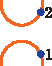
\includegraphics[scale=1]{CupCapDots.pdf}}}}}

\newcommand{\dbeta}{\mathord{\vcenter{\hbox{
\includegraphics[scale=1]{dbeta.pdf}}}}}
\newcommand{\dpsi}{\mathord{\vcenter{\hbox{
\includegraphics[scale=1]{dpsi.pdf}}}}}
\newcommand{\dblank}{\mathord{\vcenter{\hbox{
\includegraphics[scale=1]{dblank.pdf}}}}}





\newcommand{\SigmaDotDot}{\mathord{\vcenter{\hbox{
\includegraphics[scale=1]{SigmaDotDot.pdf}}}}}
\newcommand{\SigmaDotDotExchange}{\mathord{\vcenter{\hbox{
\includegraphics[scale=1]{SigmaDotDotExchange.pdf}}}}}
\newcommand{\TwoLine}{\mathord{\vcenter{\hbox{
\includegraphics[scale=1]{TwoLine.pdf}}}}}
\newcommand{\TwoLineDots}{\mathord{\vcenter{\hbox{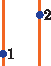
\includegraphics[scale=1]{TwoLineDots.pdf}}}}}


\newcommand{\RDotTwo}{\mathord{\vcenter{\hbox{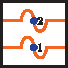
\includegraphics[scale=1]{RDotTwo.pdf}}}}}
\newcommand{\RDotTwoa}{\mathord{\vcenter{\hbox{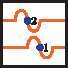
\includegraphics[scale=1]{RDotTwoa.pdf}}}}}
\newcommand{\RDotTwob}{\mathord{\vcenter{\hbox{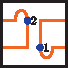
\includegraphics[scale=1]{RDotTwob.pdf}}}}}
\newcommand{\RDotTwoc}{\mathord{\vcenter{\hbox{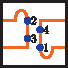
\includegraphics[scale=1]{RDotTwoc.pdf}}}}}

\newcommand{\FubeXXX}{\mathord{\vcenter{\hbox{
\includegraphics[scale=1]{EmptyTube.pdf}}}}}
\newcommand{\FubeXss}{\mathord{\vcenter{\hbox{
\includegraphics[scale=1]{OneLine.pdf}}}}}
\newcommand{\FubeXsds}{\mathord{\vcenter{\hbox{
\includegraphics[scale=1]{OneLineDot.pdf}}}}}



\newcommand{\AnnulusCut}{\mathord{\vcenter{\hbox{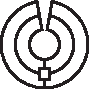
\includegraphics[scale=1]{AnnulusCut.pdf}}}}}
\newcommand{\AnnulusFlat}{\mathord{\vcenter{\hbox{
\includegraphics[scale=1]{AnnulusFlat.pdf}}}}}
\newcommand{\Disc}{\mathord{\vcenter{\hbox{
\includegraphics[scale=1]{Disc.pdf}}}}}
\newcommand{\RotatedTube}{\mathord{\vcenter{\hbox{
\includegraphics[scale=1]{RotatedTube.pdf}}}}}
\newcommand{\AnnulusGeneric}{\mathord{\vcenter{\hbox{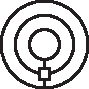
\includegraphics[scale=1]{AnnulusGeneric.pdf}}}}}

\newcommand{\DiskLarge}{\mathord{\vcenter{\hbox{
\includegraphics[scale=1]{DiskLarge.pdf}}}}}
\newcommand{\TubeIdempotentBasistrace}{\mathord{\vcenter{\hbox{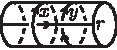
\includegraphics[scale=1]{TubeIdempotentBasistrace.pdf}}}}}


\newcommand{\FubeXXXA}{\mathord{\vcenter{\hbox{
\includegraphics[scale=1]{EmptyTubeA.pdf}}}}}
\newcommand{\FubeXssA}{\mathord{\vcenter{\hbox{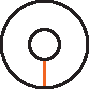
\includegraphics[scale=1]{OneLineA.pdf}}}}}
\newcommand{\FubeXsdsA}{\mathord{\vcenter{\hbox{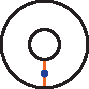
\includegraphics[scale=1]{OneLineDotA.pdf}}}}}

\newcommand{\FubesddXsA}{\mathord{\vcenter{\hbox{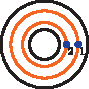
\includegraphics[scale=1]{FubesddXsA.pdf}}}}}

\newcommand{\RDotTwobA}{\mathord{\vcenter{\hbox{
\includegraphics[scale=1]{RDotTwobA.pdf}}}}}\newcommand{\RDotTwocA}{\mathord{\vcenter{\hbox{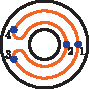
\includegraphics[scale=1]{RDotTwocA.pdf}}}}}


 
\newcommand{\Fubex}[2]{{\mathord{\ooalign{ \vphantom{$\Big|^2$}\cr\hidewidth\ensuremath{\scriptstyle{#2}}\hidewidth\cr$\vcenter{\hbox{$#1$}}$\cr
  \hidewidth\raise0ex\hbox{$\scale{1.2}{\VerticalSpace}$}\cr
  }}}}	




\newcommand{\TubeBC}{\mathord{\vcenter{\hbox{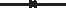
\includegraphics[scale=1]{TubeBC.pdf}}}}}

\newcommand{\TubeBCx}[1]{{\mathord{\ooalign{ \vphantom{$\Big|^2$}\cr\hidewidth\ensuremath{\scriptstyle{#1}}\hidewidth\cr$\vcenter{\hbox{$\scale{1}{\TubeBC}$}}$\cr
  \hidewidth\raise0ex\hbox{$\scale{.25}{\VerticalSpace}$}\cr
  }}}}	

\newcommand{\AnnulusBare}{\mathord{\vcenter{\hbox{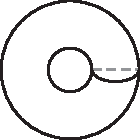
\includegraphics[scale=.6]{AnnulusBare.pdf}}}}}
\newcommand{\AnnularTube}{\mathord{\vcenter{\hbox{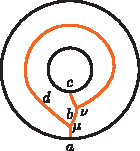
\includegraphics[scale=1]{AnnularTube.pdf}}}}}
\newcommand{\AnnularTubeNoIndex}{\mathord{\vcenter{\hbox{
\includegraphics[scale=1]{AnnularTubeNoIndex.pdf}}}}}
\newcommand{\AnnulusTubeTube}{\mathord{\vcenter{\hbox{
\includegraphics[scale=1]{AnnulusTubeTube.pdf}}}}}

\newcommand{\SAnnulusNoLabel}{\mathord{\vcenter{\hbox{
\includegraphics[scale=1]{SAnnulusNoLabel.pdf}}}}}
\newcommand{\TAnnulusNoLabel}{\mathord{\vcenter{\hbox{
\includegraphics[scale=1]{TAnnulusNoLabel.pdf}}}}}


\newcommand{\EdgeTensor}{\mathord{\vcenter{\hbox{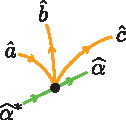
\includegraphics[scale=1]{EdgeTensor.pdf}}}}}

\newcommand{\OneHandleTheta}{\mathord{\vcenter{\hbox{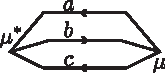
\includegraphics[scale=.7]{OneHandleTheta.pdf}}}}}
\newcommand{\OneHandlemud}{\mathord{\vcenter{\hbox{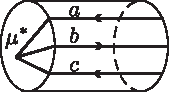
\includegraphics[scale=.7]{OneHandlemud.pdf}}}}}
\newcommand{\OneHandlemu}{\mathord{\vcenter{\hbox{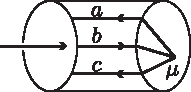
\includegraphics[scale=.7]{OneHandlemu.pdf}}}}}
\newcommand{\OneHandlea}{\mathord{\vcenter{\hbox{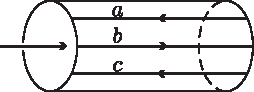
\includegraphics[scale=.7]{OneHandlea.pdf}}}}}

\newcommand{\OneHandlePrime}{\mathord{\vcenter{\hbox{\includegraphics[scale=1]{OneHandlePrime.pdf}}}}}
\newcommand{\CellDecompNearOneHandle}{\mathord{\vcenter{\hbox{\includegraphics[scale=1]{CellDecompNearOneHandle.pdf}}}}}




\newcommand{\Bilineara}{\mathord{\vcenter{\hbox{\includegraphics[scale=0.85]{Bilineara.pdf}}}}}
\newcommand{\Bilinearb}{\mathord{\vcenter{\hbox{\includegraphics[scale=0.85]{Bilinearb.pdf}}}}}
\newcommand{\Bilinearc}{\mathord{\vcenter{\hbox{\includegraphics[scale=0.85]{Bilinearc.pdf}}}}}



\newcommand{\TetrahedronPrime}{\mathord{\vcenter{\hbox{\includegraphics[scale=1]{TetrahedronPrime.pdf}}}}}
\newcommand{\Tetrahedron}{\mathord{\vcenter{\hbox{\includegraphics[scale=1]{Tetrahedron.pdf}}}}}
\newcommand{\StandardZeroCell}{\mathord{\vcenter{\hbox{\includegraphics[scale=1]{StandardZeroCell.pdf}}}}}
\newcommand{\HorshoeIdentity}{\mathord{\vcenter{\hbox{\includegraphics[scale=1]{HorshoeIdentity.pdf}}}}}

\newcommand{\PitchforkIdempotent}{\mathord{\vcenter{\hbox{\includegraphics[scale=0.7]{PitchforkIdempotent.pdf}}}}}

\newcommand{\Pitchforkabc}{\mathord{\vcenter{\hbox{\includegraphics[scale=1.3]{Pitchforkabc.pdf}}}}}
\newcommand{\Pitchforkabcrot}{\mathord{\vcenter{\hbox{\includegraphics[scale=1.3]{Pitchforkabcrot.pdf}}}}}
\newcommand{\PivotThreeTimes}{\mathord{\vcenter{\hbox{\includegraphics[scale=1.3]{PivotThreeTimes.pdf}}}}}

\newcommand{\PitchforkLarge}{\mathord{\vcenter{\hbox{\includegraphics[scale=1.3]{PitchforkLarge.pdf}}}}}
\newcommand{\Pitchforkdotthree}{\mathord{\vcenter{\hbox{\includegraphics[scale=1.3]{Pitchforkdotthree.pdf}}}}}
\newcommand{\Pitchforkdottwo}{\mathord{\vcenter{\hbox{\includegraphics[scale=1.3]{Pitchforkdottwo.pdf}}}}}
\newcommand{\Pitchforkdotone}{\mathord{\vcenter{\hbox{\includegraphics[scale=1.3]{Pitchforkdotone.pdf}}}}}






\newcommand{\FaceWeight}{\mathord{\vcenter{\hbox{\includegraphics[scale=1]{FaceWeight.pdf}}}}}
\newcommand{\EdgeTensorprime}{\mathord{\vcenter{\hbox{\includegraphics[scale=1]{EdgeTensorprime.pdf}}}}}








\newcommand{\AnnulsLabel}[5]{\mathord{ 
\mkern2mu\overset{#3}{{\Annulusxprime{#1}{#2}}}\mkern2mu\raisebox{0ex}{$\scriptstyle{#4}$} }}

\newcommand*{\Annulus}[2]{{ #1 }
\kern-3.5em\raisebox{1ex}{ $\scriptstyle{#2}$} \kern2.6em} %Could change 0 to 1.2 to raise the B.

\newcommand*{\AnnulusP}[3]{{{\Annulus{#1}{#2}} }
\kern-.5em\raisebox{3.5ex}{ $\scriptstyle{#3}$} \kern.3em} %Could change 0 to 1.2 to raise the B.

\newcommand*{\AnnulusPx}[4]{\AnnulusP{#1}{#2}{#3}
\kern-3.6em\raisebox{-4.5ex}{ $\scriptstyle{#4}$} \kern2.6em} %Could change 0 to 1.2 to raise the B.

\newcommand*{\AnularTubex}[6]{\AnnulusPx{#1}{#2}{#3}{#4}
\kern-4em\raisebox{-4.5ex}{ $\overset{#6}{\underset{#5}{\vphantom{\Big|^2}}}$} \kern3em} %Could change 0 to 1.2 to raise the B.

\newcommand*{\TorusTubex}[6]{\AnnulusPx{#1}{#2}{#3}{#4}
\kern-4em\raisebox{-4.5ex}{ $\overset{#6}{\underset{#5}{\vphantom{\Big|^2}}}$} \kern3em} %Could change 0 to 1.2 to raise the B.



\newcommand{\SAnnulusx}[3]{\mathrel{\ooalign{$\SAnnulusNoLabel$\cr
  \hidewidth\raise5ex\hbox{$\scriptstyle{#3}\mkern1mu$}\cr
  \hidewidth\raise.8ex\hbox{$\scriptstyle{#2}\mkern63mu$}\cr
    \hidewidth\raise-3.8ex\hbox{$\scriptstyle{#1}\mkern39mu$}\cr
  }}}
  
  \newcommand{\TAnnulusx}[3]{\mathrel{\ooalign{$\TAnnulusNoLabel$\cr
  \hidewidth\raise5ex\hbox{$\scriptstyle{#3}\mkern1mu$}\cr
  \hidewidth\raise.8ex\hbox{$\scriptstyle{#2}\mkern63mu$}\cr
    \hidewidth\raise-4.9ex\hbox{$\scriptstyle{#1}\mkern51mu$}\cr
  }}}

\newcommand{\AnnularTubex}[6]{\mathrel{\ooalign{$#1$\cr
  \hidewidth\raise5ex\hbox{$\scriptstyle{#6}\mkern1mu$}\cr
  \hidewidth\raise.8ex\hbox{$\scriptstyle{#5}\mkern63mu$}\cr
  \hidewidth\raise-.9ex\hbox{$\scriptstyle{#3}\mkern68mu$}\cr
    \hidewidth\raise-4.5ex\hbox{$\scriptstyle{#4} \mkern50mu$}\cr
  \hidewidth\raise-7ex\hbox{$\scriptstyle{#2}\mkern68mu$}\cr
  }}}
  




\newcommand{\AnnularTubexp}[9]{\mathrel{\ooalign{$#1$\cr
  \hidewidth\raise5ex\hbox{$\scriptstyle{#9}\mkern1mu$}\cr
 \hidewidth\raise.8ex\hbox{$\scriptstyle{#8}\mkern63mu$}\cr
  \hidewidth\raise-3.7ex\hbox{$\scriptstyle{#7}\mkern50mu$}\cr
    \hidewidth\raise-5.1ex\hbox{$\scriptstyle{#6}\mkern57mu$}\cr
  \hidewidth\raise-2.2ex\hbox{$\scriptstyle{#5}\mkern90mu$}\cr
  \hidewidth\raise-.9ex\hbox{$\scriptstyle{#4}\mkern68mu$}\cr
    \hidewidth\raise-3.8ex\hbox{$\scriptstyle{#3} \mkern69mu$}\cr
  \hidewidth\raise-7ex\hbox{$\scriptstyle{#2}\mkern68mu$}\cr
  }}}


\newcommand{\SmallTorus}[3]{\mathrel{\ooalign{$#1$\cr
  \hidewidth\raise0ex\hbox{$\scriptstyle{#2}\mkern36mu$}\cr
    \hidewidth\raise-1.5ex\hbox{$\scriptstyle{#3}\mkern10mu$}\cr
  }}}
  
  
  \newcommand{\AnnulusTubeTubex}[6]{\mathrel{\ooalign{$#1$\cr
  \hidewidth\raise.8ex\hbox{$\scriptstyle{#6}\mkern65mu$}\cr
  \hidewidth\raise-.5ex\hbox{$\scriptstyle{#3}\mkern68mu$}\cr
    \hidewidth\raise-4.9ex\hbox{$\scriptstyle{#4} \mkern50mu$}\cr
     \hidewidth\raise-2.7ex\hbox{$\scriptstyle{#5} \mkern54mu$}\cr
  \hidewidth\raise-7.3ex\hbox{$\scriptstyle{#2}\mkern68mu$}\cr
  }}}
  

  \newcommand{\Cellup}{\mathord{\vcenter{\hbox{\includegraphics[scale=1]{Cellup.pdf}}}}}
    \newcommand{\Celldown}{\mathord{\vcenter{\hbox{\includegraphics[scale=1]{Celldown.pdf}}}}}
        \newcommand{\Cellmid}{\mathord{\vcenter{\hbox{\includegraphics[scale=1]{Cellmid.pdf}}}}}
        \newcommand{\TwoCell}{\mathord{\vcenter{\hbox{\includegraphics[scale=1]{TwoCell.pdf}}}}}
                \newcommand{\Onecell}{\mathord{\vcenter{\hbox{\includegraphics[scale=1]{Onecell.pdf}}}}}      
        
        

 


\newcommand{\TorusLocalRelationc}{\mathord{\vcenter{\hbox{\includegraphics[scale=1]{TorusLocalRelationc.pdf}}}}}
\newcommand{\TorusLocalRelationb}{\mathord{\vcenter{\hbox{\includegraphics[scale=1]{TorusLocalRelationb.pdf}}}}}
\newcommand{\TorusLocalRelationa}{\mathord{\vcenter{\hbox{\includegraphics[scale=1]{TorusLocalRelationa.pdf}}}}}


\newcommand{\Dv}{\mathord{\vcenter{\hbox{\includegraphics[scale=1]{Dv.pdf}}}}}
\newcommand{\Dfv}{\mathord{\vcenter{\hbox{\includegraphics[scale=1]{Dfv.pdf}}}}}


\newcommand{\Horseshoe}{\mathord{\vcenter{\hbox{\includegraphics[scale=1]{Horseshoe.pdf}}}}}
\newcommand{\HorseshoeTwist}{\mathord{\vcenter{\hbox{\includegraphics[scale=1]{HorseshoeTwist.pdf}}}}}
\newcommand{\euv}{\mathord{\vcenter{\hbox{\includegraphics[scale=1]{euv.pdf}}}}}
\newcommand{\chieuv}{\mathord{\vcenter{\hbox{\includegraphics[scale=1]{chieuv.pdf}}}}}


\newcommand{\TubeElement}{\mathord{\vcenter{\hbox{\includegraphics[scale=1]{TubeElement.pdf}}}}}


\newcommand{\LoopOverId}{\mathord{\vcenter{\hbox{\includegraphics[scale=1]{LoopOverId.pdf}}}}}
\newcommand{\Ida}{\mathord{\vcenter{\hbox{\includegraphics[scale=1]{Ida.pdf}}}}}
\newcommand{\OmegaSLoop}{\mathord{\vcenter{\hbox{\includegraphics[scale=1]{OmegaSLoop.pdf}}}}}

\newcommand{\IdxOmegaLoopa}{\mathord{\vcenter{\hbox{\includegraphics[scale=1]{IdxOmegaLoopa.pdf}}}}}
\newcommand{\IdxOmegaLoopb}{\mathord{\vcenter{\hbox{\includegraphics[scale=1]{IdxOmegaLoopb.pdf}}}}}


\newcommand{\HandleSlidea}{\mathord{\vcenter{\hbox{\includegraphics[scale=1]{HandleSlidea.pdf}}}}}
\newcommand{\HandleSlideb}{\mathord{\vcenter{\hbox{\includegraphics[scale=1]{HandleSlideb.pdf}}}}}


\newcommand{\TubeBasisa}{\mathord{\vcenter{\hbox{\includegraphics[scale=1]{TubeBasisa.pdf}}}}}
\newcommand{\TubeBasisb}{\mathord{\vcenter{\hbox{\includegraphics[scale=1]{TubeBasisb.pdf}}}}}
\newcommand{\TubeBasisc}{\mathord{\vcenter{\hbox{\includegraphics[scale=1]{TubeBasisc.pdf}}}}}
\newcommand{\TubeBasisd}{\mathord{\vcenter{\hbox{\includegraphics[scale=1]{TubeBasisd.pdf}}}}}
\newcommand{\TubeBasisdprime}{\mathord{\vcenter{\hbox{\includegraphics[scale=1]{TubeBasisdprime.pdf}}}}}


\newcommand{\TubeBasisaF}{\mathord{\vcenter{\hbox{\includegraphics[scale=1]{TubebasisaF.pdf}}}}}
\newcommand{\TubeBasisbF}{\mathord{\vcenter{\hbox{\includegraphics[scale=1]{TubebasisbF.pdf}}}}}
\newcommand{\TubeBasiscF}{\mathord{\vcenter{\hbox{\includegraphics[scale=1]{TubebasiscF.pdf}}}}}
\newcommand{\TubeBasisdF}{\mathord{\vcenter{\hbox{\includegraphics[scale=1]{TubebasisdF.pdf}}}}}

\newcommand{\TubeFiga}{\mathord{\vcenter{\hbox{\includegraphics[scale=1]{TubeFiga.pdf}}}}}
\newcommand{\TubeFigb}{\mathord{\vcenter{\hbox{\includegraphics[scale=1]{TubeFigb.pdf}}}}}
\newcommand{\TubeFigc}{\mathord{\vcenter{\hbox{\includegraphics[scale=1]{TubeFigc.pdf}}}}}


 
\newcommand{\gxyajf}{\mathord{\vcenter{\hbox{\includegraphics[scale=1]{gxyajf.pdf}}}}}
\newcommand{\hxyaif}{\mathord{\vcenter{\hbox{\includegraphics[scale=1]{hxyaif.pdf}}}}}



\newcommand{\OneStrandIdempotentMTCpsi}{\mathord{\vcenter{\hbox{\includegraphics[scale=1]{OneStrandIdempotentMTC.pdf}}}}}
\newcommand{\gxyaj}{\mathord{\vcenter{\hbox{\includegraphics[scale=1]{gxyaj.pdf}}}}}
\newcommand{\hxyai}{\mathord{\vcenter{\hbox{\includegraphics[scale=1]{hxyai.pdf}}}}}

\newcommand{\VxyaoVxya}{\mathord{\vcenter{\hbox{\includegraphics[scale=1]{VxyaoVxya.pdf}}}}}
\newcommand{\idaprime}{\mathord{\vcenter{\hbox{\includegraphics[scale=1]{idaprime.pdf}}}}}

\newcommand{\Vxyxy}{\mathord{\vcenter{\hbox{\includegraphics[scale=1]{Vxyxy.pdf}}}}}
\newcommand{\idxy}{\mathord{\vcenter{\hbox{\includegraphics[scale=1]{idxy.pdf}}}}}
\newcommand{\Vxyxyomega}{\mathord{\vcenter{\hbox{\includegraphics[scale=1]{Vxyxyomega.pdf}}}}}



\newcommand{\SpinStructureProjector}{\mathord{\vcenter{\hbox{\includegraphics[scale=1]{SpinStructureProjector.pdf}}}}}


\newcommand{\EmptyTubeW}{\mathord{\vcenter{\hbox{\includegraphics[scale=1]{EmptyTubeW.pdf}}}}}

\newcommand{\TubeProject}{\mathord{\vcenter{\hbox{\includegraphics[scale=1]{TubeProject.pdf}}}}}


\newcommand{\TuberraJ}{\mathord{\vcenter{\hbox{\includegraphics[scale=1]{TuberraJ.pdf}}}}}
\newcommand{\Tubeidr}{\mathord{\vcenter{\hbox{\includegraphics[scale=1]{Tubeidr.pdf}}}}}
\newcommand{\Tuberr}{\mathord{\vcenter{\hbox{\includegraphics[scale=1]{Tuberr.pdf}}}}}


\newcommand{\TuberrTraceCe}{\mathord{\vcenter{\hbox{\includegraphics[scale=1]{TuberrTraceCe.pdf}}}}}
\newcommand{\TuberrTraceCo}{\mathord{\vcenter{\hbox{\includegraphics[scale=1]{TuberrTraceCo.pdf}}}}}

\newcommand{\Tuberrprime}{\mathord{\vcenter{\hbox{\includegraphics[scale=1]{Tuberrprime.pdf}}}}}
\newcommand{\Tuberrprimecut}{\mathord{\vcenter{\hbox{\includegraphics[scale=1]{Tuberrprimecut.pdf}}}}}
\newcommand{\PinchedDisk}{\mathord{\vcenter{\hbox{\includegraphics[scale=1]{PinchedDisk.pdf}}}}}

\newcommand{\clx}{\mathord{\vcenter{\hbox{\includegraphics[scale=1]{clx.pdf}}}}}


\newcommand{\Tuberrprimenolabel}{\mathord{\vcenter{\hbox{\includegraphics[scale=1]{Tuberrprimenolabel.pdf}}}}}

\newcommand{\moronex}{\mathord{\vcenter{\hbox{\includegraphics[scale=1]{moronex.pdf}}}}}
\newcommand{\moronexj}{\mathord{\vcenter{\hbox{\includegraphics[scale=1]{moronexj.pdf}}}}}



\newcommand{\moronexcollar}{\mathord{\vcenter{\hbox{\includegraphics[scale=1]{moronexcollar.pdf}}}}}




\newcommand{\exyomegaa}{\mathord{\vcenter{\hbox{\includegraphics[scale=1]{exyomegaa.pdf}}}}}
\newcommand{\exyomegab}{\mathord{\vcenter{\hbox{\includegraphics[scale=1]{exyomegab.pdf}}}}}
\newcommand{\exyomegac}{\mathord{\vcenter{\hbox{\includegraphics[scale=1]{exyomegac.pdf}}}}}

\newcommand{\EFunctora}{\mathord{\vcenter{\hbox{\includegraphics[scale=1]{EFunctora.pdf}}}}}
\newcommand{\EFunctorb}{\mathord{\vcenter{\hbox{\includegraphics[scale=1]{EFunctorb.pdf}}}}}
\newcommand{\EFunctorc}{\mathord{\vcenter{\hbox{\includegraphics[scale=1]{EFunctorc.pdf}}}}}


\newcommand{\IdempotentBasis}{\mathord{\vcenter{\hbox{\includegraphics[scale=1]{IdempotentBasis.pdf}}}}}

\newcommand{\TubeIdempotentTwoStrand}{\mathord{\vcenter{\hbox{\includegraphics[scale=1]{TubeIdempotentTwoStrand.pdf}}}}}
\newcommand{\fTubeCf}{\mathord{\vcenter{\hbox{\includegraphics[scale=1]{fTubeCf.pdf}}}}}
\newcommand{\fTubefOdd}{\mathord{\vcenter{\hbox{\includegraphics[scale=1]{fTubefOdd.pdf}}}}}
\newcommand{\minimalBosonic}{\mathord{\vcenter{\hbox{\includegraphics[scale=1]{minimalBosonic.pdf}}}}}

\newcommand{\TubeIdempotentTwoStrandab}{\mathord{\vcenter{\hbox{\includegraphics[scale=1]{TubeIdempotentTwoStrandab.pdf}}}}}
\newcommand{\BasisForIdempotents}{\mathord{\vcenter{\hbox{\includegraphics[scale=1]{BasisForIdempotents.pdf}}}}}

\newcommand{\minimalBosonicRHS}{\mathord{\vcenter{\hbox{\includegraphics[scale=1]{minimalBosonicRHS.pdf}}}}}
\newcommand{\ftubefOddRHS}{\mathord{\vcenter{\hbox{\includegraphics[scale=1]{ftubefOddRHS.pdf}}}}}




\newcommand{\FusionIsomorphism}{\mathord{\vcenter{\hbox{\includegraphics[scale=1]{FusionIsomorphism.pdf}}}}}

\newcommand{\FusionIsomorphismprimereduced}{\mathord{\vcenter{\hbox{\includegraphics[scale=1]{FusionIsomorphismprimereduced.pdf}}}}}
\newcommand{\FusionIsomorphismprime}{\mathord{\vcenter{\hbox{\includegraphics[scale=1]{FusionIsomorphismprime.pdf}}}}}



\newcommand{\TubeCompletea}{\mathord{\vcenter{\hbox{\includegraphics[scale=1]{TubeCompletea.pdf}}}}}
\newcommand{\TubeCompleteb}{\mathord{\vcenter{\hbox{\includegraphics[scale=1]{TubeCompleteb.pdf}}}}}
\newcommand{\TubeCompletec}{\mathord{\vcenter{\hbox{\includegraphics[scale=1]{TubeCompletec.pdf}}}}}
\newcommand{\TubeCompletecprime}{\mathord{\vcenter{\hbox{\includegraphics[scale=1]{TubeCompletecprime.pdf}}}}}



\newcommand{\Ufghk}{\mathord{\vcenter{\hbox{\includegraphics[scale=1]{Ufghk.pdf}}}}}


\newcommand{\fxyaJ}{\mathord{\vcenter{\hbox{\includegraphics[scale=1]{fxyaJ.pdf}}}}}


\newcommand{\TubeTwotoOneStrand}{\mathord{\vcenter{\hbox{\includegraphics[scale=1]{TubeTwotoOneStrand.pdf}}}}}
\newcommand{\TubeOnetoTwoStrand}{\mathord{\vcenter{\hbox{\includegraphics[scale=1]{TubeOnetoTwoStrand.pdf}}}}}
 

\newcommand{\SMatrix}[2]{\mathrel{\ooalign{$\OmegaSLoop$\cr
  \hidewidth\raise0ex\hbox{$\scriptstyle{#1}\mkern18mu$}\cr
    \hidewidth\raise0ex\hbox{$\scriptstyle{#2}\mkern-10mu$}\cr
  }}}
  
  
  \newcommand{\SMatrixx}[2]{\mathrel{\ooalign{$\OmegaSLoop$\cr
  \hidewidth\raise0ex\hbox{$\scriptstyle{#1}\mkern12mu$}\cr
    \hidewidth\raise0ex\hbox{$\scriptstyle{#2}\mkern-10mu$}\cr
  }}}
  
  
  \newcommand{\SMatrixxx}[2]{\mathrel{\ooalign{$\OmegaSLoop$\cr
  \hidewidth\raise0ex\hbox{$\scriptstyle{#1}\mkern12mu$}\cr
    \hidewidth\raise0ex\hbox{$\scriptstyle{#2}\mkern-38mu$}\cr
  }}}

  
  
  \newcommand{\OmegaLoopDefectx}[2]{\mathrel{\ooalign{$\OmegaLoopDefect$\cr
  \hidewidth\raise0ex\hbox{$\scriptstyle{#1}\mkern8mu$}\cr
    \hidewidth\raise0ex\hbox{$\scriptstyle{#2}\mkern-22mu$}\cr
  }}}
  
  \newcommand{\OmegaLoopDefect}{\mathord{\vcenter{\hbox{\includegraphics[scale=1]{OmegaLoopDefect.pdf}}}}}
    \newcommand{\DiscGray}{\mathord{\vcenter{\hbox{\includegraphics[scale=1]{DiscGray.pdf}}}}}
    
    
    
\newcommand{\DCSmatrixf}{\mathord{\vcenter{\hbox{\includegraphics[scale=1]{DCSmatrixf.pdf}}}}}
\newcommand{\DCSmatrixa}{\mathord{\vcenter{\hbox{\includegraphics[scale=1]{DCSmatrixa.pdf}}}}}
\newcommand{\DCSmatrixb}{\mathord{\vcenter{\hbox{\includegraphics[scale=1]{DCSmatrixb.pdf}}}}}\newcommand{\DCSmatrixc}{\mathord{\vcenter{\hbox{\includegraphics[scale=1]{DCSmatrixc.pdf}}}}}
\newcommand{\DCSmatrixd}{\mathord{\vcenter{\hbox{\includegraphics[scale=1]{DCSmatrixd.pdf}}}}}
\newcommand{\DCSmatrixe}{\mathord{\vcenter{\hbox{\includegraphics[scale=1]{DCSmatrixe.pdf}}}}}

\newcommand{\DCSmatrixg}{\mathord{\vcenter{\hbox{\includegraphics[scale=1]{DCSmatrixg.pdf}}}}}
\newcommand{\DCSmatrixh}{\mathord{\vcenter{\hbox{\includegraphics[scale=1]{DCSmatrixh.pdf}}}}}


\newcommand{\STorusBasisa}{\mathord{\vcenter{\hbox{\includegraphics[scale=1]{STorusBasisa.pdf}}}}}


\newcommand{\Scalcae}{\mathord{\vcenter{\hbox{\includegraphics[scale=1]{Scalcae.pdf}}}}}  
\newcommand{\Scalcad}{\mathord{\vcenter{\hbox{\includegraphics[scale=1]{Scalcad.pdf}}}}}  
\newcommand{\Scalcac}{\mathord{\vcenter{\hbox{\includegraphics[scale=1]{Scalcac.pdf}}}}}  
\newcommand{\Scalcab}{\mathord{\vcenter{\hbox{\includegraphics[scale=1]{Scalcab.pdf}}}}}
\newcommand{\Scalcaa}{\mathord{\vcenter{\hbox{\includegraphics[scale=1]{Scalcaa.pdf}}}}}  


\newcommand{\Scalcbe}{\mathord{\vcenter{\hbox{\includegraphics[scale=1]{Scalcbe.pdf}}}}}  
\newcommand{\Scalcbd}{\mathord{\vcenter{\hbox{\includegraphics[scale=1]{Scalcbd.pdf}}}}}  
\newcommand{\Scalcbc}{\mathord{\vcenter{\hbox{\includegraphics[scale=1]{Scalcbc.pdf}}}}}  
\newcommand{\Scalcbb}{\mathord{\vcenter{\hbox{\includegraphics[scale=1]{Scalcbb.pdf}}}}}
\newcommand{\Scalcba}{\mathord{\vcenter{\hbox{\includegraphics[scale=1]{Scalcba.pdf}}}}}  


\newcommand{\Scalcbedot}{\mathord{\vcenter{\hbox{\includegraphics[scale=1]{Scalcbedot.pdf}}}}}  
\newcommand{\Scalcbddot}{\mathord{\vcenter{\hbox{\includegraphics[scale=1]{Scalcbddot.pdf}}}}}  
\newcommand{\Scalcbadot}{\mathord{\vcenter{\hbox{\includegraphics[scale=1]{Scalcbadot.pdf}}}}}    

\newcommand{\Scalcbddotprime}{\mathord{\vcenter{\hbox{\includegraphics[scale=1]{Scalcbddotprime.pdf}}}}}
\newcommand{\Scalcbadotprime}{\mathord{\vcenter{\hbox{\includegraphics[scale=1]{Scalcbadotprime.pdf}}}}}

\newcommand{\Szmatrix}{\mathord{\vcenter{\hbox{\includegraphics[scale=1]{Szmatrix.pdf}}}}}

 

  
\newcommand{\LoopArrow}{\mathord{\vcenter{\hbox{\includegraphics[scale=1]{LoopArrow.pdf}}}}}  
\newcommand{\LoopArrowx}[1]{\mathrel{\ooalign{$\LoopArrow_{\mathrel{\raisebox{4pt}{$\scriptstyle{#1}$}}}$
  }}}
  
  
\newcommand{\OmegaLoop}{\mathord{\vcenter{\hbox{\includegraphics[scale=1]{OmegaLoop.pdf}}}}}  
\newcommand{\OmegaLoopx}[1]{\mathrel{\ooalign{$\OmegaLoop_{\mathrel{\raisebox{4pt}{$\scriptstyle{#1}$}}}$
  }}}



\newcommand{\TubeElementx}[3]{\mathrel{\ooalign{$\TubeElement$\cr
  \hidewidth\raise-3.55ex\hbox{$\scriptstyle{#1}\mkern62mu$}\cr
        \hidewidth\raise-6.3ex\hbox{$\scriptstyle{#2}\mkern61mu$}\cr
                \hidewidth\raise-0.3ex\hbox{$\scriptstyle{#3}\mkern60mu$}\cr
          \hidewidth\raise0ex\hbox{$\scale{1.5}{\VerticalSpace}$}\cr
  }}}

\newcommand{\IdempotentMTCNoLabel}{\mathord{\vcenter{\hbox{\includegraphics[scale=1]{IdempotentMTC.pdf}}}}}
\newcommand{\IdempBraid}[5]{\mathrel{\ooalign{$\IdempotentMTCNoLabel$\cr
  \hidewidth\raise-4.3ex\hbox{$\scriptstyle{#1}\mkern78mu$}\cr
    \hidewidth\raise-4.3ex\hbox{$\scriptstyle{#2}\mkern43mu$}\cr
        \hidewidth\raise-6.3ex\hbox{$\scriptstyle{#3}\mkern61mu$}\cr
        \hidewidth\raise4.1ex\hbox{$\scriptstyle{#4}\mkern25mu$}\cr
                \hidewidth\raise0ex\hbox{$\scriptstyle{#5}\mkern60mu$}\cr
          \hidewidth\raise0ex\hbox{$\scale{1.5}{\VerticalSpace}$}\cr
  }}}
  
\newcommand{\TorusBasisMTCNoLabel}{\mathord{\vcenter{\hbox{\includegraphics[scale=1]{TorusBasisMTC.pdf}}}}}
\newcommand{\TorusBraidBasis}[6]{\mathrel{\ooalign{$\TorusBasisMTCNoLabel$\cr
  \hidewidth\raise-4.3ex\hbox{$\scriptstyle{#1}\mkern78mu$}\cr
    \hidewidth\raise-4.3ex\hbox{$\scriptstyle{#2}\mkern40mu$}\cr
        \hidewidth\raise-6.3ex\hbox{$\scriptstyle{#3}\mkern61mu$}\cr
        \hidewidth\raise4.1ex\hbox{$\scriptstyle{#4}\mkern25mu$}\cr
                \hidewidth\raise0ex\hbox{$\scriptstyle{#5}\mkern58mu$}\cr
                                \hidewidth\raise4.7ex\hbox{$\scriptstyle{#6}\mkern0mu$}\cr
          \hidewidth\raise0ex\hbox{$\scale{1.5}{\VerticalSpace}$}\cr
  }}}
  
  \newcommand{\tcca}{\mathord{\vcenter{\hbox{\includegraphics[scale=1]{tcca.pdf}}}}}
    \newcommand{\tccb}{\mathord{\vcenter{\hbox{\includegraphics[scale=1]{tccb.pdf}}}}}
     \newcommand{\tccc}{\mathord{\vcenter{\hbox{\includegraphics[scale=1]{tccc.pdf}}}}}
      \newcommand{\tccd}{\mathord{\vcenter{\hbox{\includegraphics[scale=1]{tccd.pdf}}}}}
   
  
 


\newcommand{\TorusBasisMTCdl}{\mathord{\vcenter{\hbox{\includegraphics[scale=1]{TorusBasisMTCdl.pdf}}}}}
\newcommand{\TorusBasisMTCdr}{\mathord{\vcenter{\hbox{\includegraphics[scale=1]{TorusBasisMTCdr.pdf}}}}}
\newcommand{\TorusBasisMTCdd}{\mathord{\vcenter{\hbox{\includegraphics[scale=1]{TorusBasisMTCdd.pdf}}}}}
 
 \newcommand{\TorusBraidBasisd}[7]{\mathrel{\ooalign{$#7$\cr
  \hidewidth\raise-4.3ex\hbox{$\scriptstyle{#1}\mkern78mu$}\cr
    \hidewidth\raise-4.3ex\hbox{$\scriptstyle{#2}\mkern40mu$}\cr
        \hidewidth\raise-6.3ex\hbox{$\scriptstyle{#3}\mkern61mu$}\cr
        \hidewidth\raise4.1ex\hbox{$\scriptstyle{#4}\mkern25mu$}\cr
                \hidewidth\raise0ex\hbox{$\scriptstyle{#5}\mkern58mu$}\cr
                                \hidewidth\raise4.7ex\hbox{$\scriptstyle{#6}\mkern0mu$}\cr
          \hidewidth\raise0ex\hbox{$\scale{1.5}{\VerticalSpace}$}\cr
  }}}



\newcommand{\TaddownTubeNoLabel}{\mathord{\vcenter{\hbox{\includegraphics[scale=1]{TaddownTube.pdf}}}}}
\newcommand{\TadupTubeNoLabel}{\mathord{\vcenter{\hbox{\includegraphics[scale=1]{TadupTube.pdf}}}}}
\newcommand{\hTube}{\mathord{\vcenter{\hbox{\includegraphics[scale=1]{hTube.pdf}}}}}
\newcommand{\tTube}{\mathord{\vcenter{\hbox{\includegraphics[scale=1]{tTube.pdf}}}}}
\newcommand{\eTube}{\mathord{\vcenter{\hbox{\includegraphics[scale=1]{eTube.pdf}}}}}
\newcommand{\vTube}{\mathord{\vcenter{\hbox{\includegraphics[scale=1]{vTube.pdf}}}}}


\newcommand{\dota}{\mathord{\vcenter{\hbox{\includegraphics[scale=1]{dota.pdf}}}}}
\newcommand{\dotb}{\mathord{\vcenter{\hbox{\includegraphics[scale=1]{dotb.pdf}}}}}
\newcommand{\dotc}{\mathord{\vcenter{\hbox{\includegraphics[scale=1]{dotc.pdf}}}}}

\newcommand{\XTubeNoLabel}{\mathord{\vcenter{\hbox{\includegraphics[scale=1]{XTube.pdf}}}}}
\newcommand{\XTube}[2]{\mathrel{\ooalign{$\XTubeNoLabel$\cr
  \hidewidth\raise-2.5ex\hbox{$\scriptstyle{#2}\mkern28mu$}\cr
    \hidewidth\raise-2.9ex\hbox{$\scriptstyle{#1}\mkern50mu$}\cr
  }}}


\newcommand{\TaddownTube}[1]{\mathrel{\ooalign{$\TaddownTubeNoLabel$\cr
    \hidewidth\raise-2.8ex\hbox{$\scriptstyle{#1}\mkern30mu$}\cr
  }}}
  
  
  
  \newcommand{\TaddownTubeprime}[1]{\mathrel{\ooalign{$\TaddownTubeNoLabel$\cr
    \hidewidth\raise-3.0ex\hbox{$\scriptstyle{#1}\mkern32mu$}\cr
  }}}
  
  \newcommand{\TadupTube}[1]{\mathrel{\ooalign{$\TadupTubeNoLabel$\cr
    \hidewidth\raise-2.8ex\hbox{$\scriptstyle{#1}\mkern30mu$}\cr
  }}}
  
  \newcommand{\TorusNoLabels}{\mathord{\vcenter{\hbox{\includegraphics[scale=1]{TorusNoLabels.pdf}}}}}
\newcommand{\TorusNoLabelsx}[1]{\mathrel{\ooalign{$\TorusNoLabels$\cr
    \hidewidth\raise-2.8ex\hbox{$\scriptstyle{#1}\mkern30mu$}\cr
  }}}

\newcommand{\VerticalSpace}{\mathord{\vcenter{\hbox{\includegraphics[scale=1]{VerticalSpace.pdf}}}}}

\newcommand{\AddDat}[3]{\mathrel{\ooalign{  $#1$\cr
  \hidewidth\raise0ex\hbox{$\scriptstyle{#2}\mkern38mu$}\cr
  \hidewidth\raise0ex\hbox{${#3}\mkern0mu$}\cr
  \hidewidth\raise0ex\hbox{$\VerticalSpace$}\cr
  }}}
  
  \newcommand{\AddDatTorus}[3]{\mathrel{\ooalign{  $#1$\cr
  \hidewidth\raise0ex\hbox{$\scriptstyle{#2}\mkern38mu$}\cr
  \hidewidth\raise3.8ex\hbox{$\scriptstyle{#3}\mkern0mu$}\cr
  \hidewidth\raise0ex\hbox{$\VerticalSpace$}\cr
  }}}
  
    \newcommand{\AddDatTorusDot}[4]{\mathrel{\ooalign{  $#1$\cr
  \hidewidth\raise0ex\hbox{$\scriptstyle{#2}\mkern38mu$}\cr
  \hidewidth\raise3.8ex\hbox{$\scriptstyle{#3}\mkern0mu$}\cr
  \hidewidth\raise0ex\hbox{${#4}\mkern0mu$}\cr
  \hidewidth\raise0ex\hbox{$\VerticalSpace$}\cr
  }}}
  
  
  
 
  
   
  \newcommand{\TubeProductCoefficienta}{\mathord{\vcenter{\hbox{\includegraphics[scale=1]{TubeProductCoefficienta.pdf}}}}}
  \newcommand{\TubeProductCoefficientb}{\mathord{\vcenter{\hbox{\includegraphics[scale=1]{TubeProductCoefficientb.pdf}}}}}
  
    \newcommand{\ThetaSymbol}{\mathord{\vcenter{\hbox{\includegraphics[scale=1]{Theta.pdf}}}}}
 
   \newcommand{\ThetaSymbolx}[1]{\mathrel{\ooalign{$\ThetaSymbol$\cr
      \hidewidth\raise-1.3ex\hbox{$\scriptstyle{#1} \mkern0mu$}\cr
  }}}
  
  
    
  \newcommand{\TubeProductCoefficientbx}[2]{\mathrel{\ooalign{$\TubeProductCoefficientb \;\;\; $\cr
      \hidewidth\raise-.8ex\hbox{$\scriptstyle{#1} \mkern54mu$}\cr
      \hidewidth\raise-.8ex\hbox{$\scriptstyle{#2} \mkern6mu$}\cr
  }}}
  
  \newcommand{\TubeProductCoefficientax}[5]{\mathrel{\ooalign{$\TubeProductCoefficienta$\cr
      \hidewidth\raise-4.2ex\hbox{$\scriptstyle{#1} \mkern30mu$}\cr
      \hidewidth\raise-1.8ex\hbox{$\scriptstyle{#2} \mkern30mu$}\cr
  \hidewidth\raise6.1ex\hbox{$\scriptstyle{#3}\mkern44mu$}\cr
  \hidewidth\raise2.05ex\hbox{$\scriptstyle{#4}\mkern82mu$}\cr
    \hidewidth\raise3.2ex\hbox{$\scriptstyle{#5}\mkern3mu$}\cr
  }}}

  

  
    
\newcommand{\tubex}[8]{#1 \left(\substack{#8\\ \\ #5\\ } \; \substack{#4\\ #3\\ #2\\ }\; \substack{ #7 \\ #6} \right)}


\newcommand{\FubesXs}{\mathord{\vcenter{\hbox{\includegraphics[scale=1,angle=90,origin=c]{OneLine.pdf}}}}}
\newcommand{\FubesdXs}{\mathord{\vcenter{\hbox{\includegraphics[scale=1]{FubesdXs.pdf}}}}}

\newcommand{\FubessX}{\mathord{\vcenter{\hbox{\includegraphics[scale=1]{FubessX.pdf}}}}}
\newcommand{\FubessdX}{\mathord{\vcenter{\hbox{\includegraphics[scale=1]{FubessdX.pdf}}}}}

\newcommand{\FubesdXsA}{\mathord{\vcenter{\hbox{\includegraphics[scale=1]{FubesdXsA.pdf}}}}}
\newcommand{\FubessXA}{\mathord{\vcenter{\hbox{\includegraphics[scale=1]{FubessXA.pdf}}}}}
\newcommand{\FubessdXA}{\mathord{\vcenter{\hbox{\includegraphics[scale=1]{FubessdXA.pdf}}}}}


\newcommand{\FubesXsA}{\mathord{\vcenter{\hbox{\includegraphics[scale=1]{FubesXshA.pdf}}}}}
\newcommand{\FubesXsa}{\mathord{\vcenter{\hbox{\includegraphics[scale=1]{FubesXsa.pdf}}}}}
\newcommand{\FubesXsb}{\mathord{\vcenter{\hbox{\includegraphics[scale=1]{FubesXsb.pdf}}}}}
\newcommand{\FubesXsc}{\mathord{\vcenter{\hbox{\includegraphics[scale=1]{FubesXsc.pdf}}}}}


\newcommand{\FubesXscA}{\mathord{\vcenter{\hbox{\includegraphics[scale=1]{FubeXscA.pdf}}}}}
\newcommand{\FubesXsbA}{\mathord{\vcenter{\hbox{\includegraphics[scale=1]{FubeXsbA.pdf}}}}}
\newcommand{\FubesXsaA}{\mathord{\vcenter{\hbox{\includegraphics[scale=1]{FubeXsaA.pdf}}}}}






\newcommand{\qqo}{\mathord{\vcenter{\hbox{\includegraphics[scale=.4]{qq1.pdf}}}}}
\newcommand{\qtqo}{\mathord{\vcenter{\hbox{\includegraphics[scale=.4]{qtq1.pdf}}}}}
\newcommand{\qqto}{\mathord{\vcenter{\hbox{\includegraphics[scale=.4]{qqt1.pdf}}}}}
\newcommand{\qtqto}{\mathord{\vcenter{\hbox{\includegraphics[scale=.4]{qtqt1.pdf}}}}}
\newcommand{\qqm}{\mathord{\vcenter{\hbox{\includegraphics[scale=.4]{qqm.pdf}}}}}
\newcommand{\qtqm}{\mathord{\vcenter{\hbox{\includegraphics[scale=.4]{qtqm.pdf}}}}}
\newcommand{\qqtm}{\mathord{\vcenter{\hbox{\includegraphics[scale=.4]{qqtm.pdf}}}}}
\newcommand{\qtqtm}{\mathord{\vcenter{\hbox{\includegraphics[scale=.4]{qtqtm.pdf}}}}}

\newcommand{\PantsPAP}{\mathord{\vcenter{\hbox{\includegraphics[scale=0.7]{PantsPAP.pdf}}}}}
\newcommand{\PantsPAsP}{\mathord{\vcenter{\hbox{\includegraphics[scale=0.7]{PantsPAsP.pdf}}}}}

\newcommand{\PantsPsdAP}{\mathord{\vcenter{\hbox{\includegraphics[scale=0.7]{PantsPsdAP.pdf}}}}}
\newcommand{\PantsPsdAsP}{\mathord{\vcenter{\hbox{\includegraphics[scale=0.7]{PantsPsdAsP.pdf}}}}}



\newcommand{\PantsPPA}{\mathord{\vcenter{\hbox{\includegraphics[scale=0.7]{PantsPPA.pdf}}}}}
\newcommand{\PantsPPAs}{\mathord{\vcenter{\hbox{\includegraphics[scale=0.7]{PantsPPAs.pdf}}}}}

\newcommand{\PantsAsAshAsvt}{\mathord{\vcenter{\hbox{\includegraphics[scale=0.7]{PantsAsAshAsvt.pdf}}}}}
\newcommand{\PantsAstAAs}{\mathord{\vcenter{\hbox{\includegraphics[scale=0.7]{PantsAstAAs.pdf}}}}}

\newcommand{\PantsAstAshAs}{\mathord{\vcenter{\hbox{\includegraphics[scale=0.7]{PantsAstAshAs.pdf}}}}}
\newcommand{\PantsAsAshAs}{\mathord{\vcenter{\hbox{\includegraphics[scale=0.7]{PantsAsAshAs.pdf}}}}}
\newcommand{\PantsAsAAs}{\mathord{\vcenter{\hbox{\includegraphics[scale=0.7]{PantsAsAAs.pdf}}}}}

\newcommand{\Pantssvtsvtsh}{\mathord{\vcenter{\hbox{\includegraphics[scale=.7,origin=c]{Pantssvtsvtsh.pdf}}}}}
\newcommand{\Pantssvtsvsh}{\mathord{\vcenter{\hbox{\includegraphics[scale=.7,angle=0,origin=c]{Pantssvtsvsh.pdf}}}}}
\newcommand{\Pantssvsvtsh}{\mathord{\vcenter{\hbox{\includegraphics[scale=.7,angle=0,origin=c]{Pantssvsvtsh.pdf}}}}}
\newcommand{\Pantssvsvsh}{\mathord{\vcenter{\hbox{\includegraphics[scale=.7,angle=0,origin=c]{Pantssvsvsh.pdf}}}}}
\newcommand{\PantssvtsvtX}{\mathord{\vcenter{\hbox{\includegraphics[scale=.7,angle=0,origin=c]{PantssvtsvtX.pdf}}}}}
\newcommand{\PantssvtsvX}{\mathord{\vcenter{\hbox{\includegraphics[scale=.7,angle=0,origin=c]{PantssvtsvX.pdf}}}}}

\newcommand{\PantssvsvtX}{\mathord{\vcenter{\hbox{\includegraphics[scale=.7,angle=0,origin=c]{PantssvsvtX.pdf}}}}}
\newcommand{\PantssvsvX}{\mathord{\vcenter{\hbox{\includegraphics[scale=.7,angle=0,origin=c]{PantssvsvX.pdf}}}}}

\newcommand{\PantssvtXsvd}{\mathord{\vcenter{\hbox{\includegraphics[scale=.7,angle=0,origin=c]{PantssvtXsvd.pdf}}}}}
\newcommand{\Pantssvtshsvd}{\mathord{\vcenter{\hbox{\includegraphics[scale=.7,angle=0,origin=c]{Pantssvtshsvd.pdf}}}}}
\newcommand{\Pantssvshsvd}{\mathord{\vcenter{\hbox{\includegraphics[scale=.7,angle=0,origin=c]{Pantssvshsvd.pdf}}}}}
\newcommand{\PantssvXsvd}{\mathord{\vcenter{\hbox{\includegraphics[scale=.7,angle=0,origin=c]{PantssvXsvd.pdf}}}}}

\newcommand{\PantssvtXsvt}{\mathord{\vcenter{\hbox{\includegraphics[scale=.7,angle=0,origin=c]{PantssvtXsvt.pdf}}}}}
\newcommand{\PantssvXsvt}{\mathord{\vcenter{\hbox{\includegraphics[scale=.7,angle=0,origin=c]{PantssvXsvt.pdf}}}}}

\newcommand{\PantssvtXsv}{\mathord{\vcenter{\hbox{\includegraphics[scale=.7,angle=0,origin=c]{PantssvtXsv.pdf}}}}}



%%%%%%%%%%%%%%%%%%%%%%%%%%%%%%%%%%%%%%%%%%%%%%%%
%%%%%%%%%%%%%%%%%%%%%%%%%%%%%%%%%%%%%%%%%%%%%%%%
\newcommand{\PantssvXsvdA}{\mathord{\vcenter{\hbox{\includegraphics[scale=.8,angle=0,origin=c]{PantssvXsvdA.pdf}}}}}
\newcommand{\PantssvtXsvdA}{\mathord{\vcenter{\hbox{\includegraphics[scale=.8,angle=0,origin=c]{PantssvtXsvdA.pdf}}}}}
\newcommand{\PantssvtshsvdA}{\mathord{\vcenter{\hbox{\includegraphics[scale=.8,angle=0,origin=c]{PantssvtshsvdA.pdf}}}}}
\newcommand{\PantssvshsvdA}{\mathord{\vcenter{\hbox{\includegraphics[scale=.8,angle=0,origin=c]{PantssvshsvdA.pdf}}}}}
\newcommand{\PantsPsdAsPA}{\mathord{\vcenter{\hbox{\includegraphics[scale=.8,angle=0,origin=c]{PantsPsdAsPA.pdf}}}}}
\newcommand{\PantsPsdAPA}{\mathord{\vcenter{\hbox{\includegraphics[scale=.8,angle=0,origin=c]{PantsPsdAPA.pdf}}}}}
\newcommand{\PantsPPAsA}{\mathord{\vcenter{\hbox{\includegraphics[scale=.8,angle=0,origin=c]{PantsPPAsA.pdf}}}}}
\newcommand{\PantsPPAA}{\mathord{\vcenter{\hbox{\includegraphics[scale=.8,angle=0,origin=c]{PantsPPAA.pdf}}}}}
\newcommand{\PantsPAsPA}{\mathord{\vcenter{\hbox{\includegraphics[scale=.8,angle=0,origin=c]{PantsPAsPA.pdf}}}}}
\newcommand{\PantsPAPA}{\mathord{\vcenter{\hbox{\includegraphics[scale=.8,angle=0,origin=c]{PantsPAPA.pdf}}}}}
\newcommand{\PantsAstAAsA}{\mathord{\vcenter{\hbox{\includegraphics[scale=.8,angle=0,origin=c]{PantsAstAAsA.pdf}}}}}
\newcommand{\PantsAsAshAsvtA}{\mathord{\vcenter{\hbox{\includegraphics[scale=.8,angle=0,origin=c]{PantsAsAshAsvtA.pdf}}}}}
\newcommand{\PantsNNda}{\mathord{\vcenter{\hbox{\includegraphics[scale=.8,angle=0,origin=c]{PantsNNda.pdf}}}}}
\newcommand{\PantsNNd}{\mathord{\vcenter{\hbox{\includegraphics[scale=.8,angle=0,origin=c]{PantsNNd.pdf}}}}}

\newcommand{\Pantsmsixa}{\mathord{\vcenter{\hbox{\includegraphics[scale=.8,angle=0,origin=c]{Pantsmsixa.pdf}}}}}
\newcommand{\Pantsmsixb}{\mathord{\vcenter{\hbox{\includegraphics[scale=.8,angle=0,origin=c]{Pantsmsixb.pdf}}}}}
\newcommand{\Pantsmsixc}{\mathord{\vcenter{\hbox{\includegraphics[scale=.8,angle=0,origin=c]{Pantsmsixc.pdf}}}}}
\newcommand{\Pantsmsixd}{\mathord{\vcenter{\hbox{\includegraphics[scale=.8,angle=0,origin=c]{Pantsmsixd.pdf}}}}}

\newcommand{\Pantsmsixe}{\mathord{\vcenter{\hbox{\includegraphics[scale=.8,angle=0,origin=c]{Pantsmsixe.pdf}}}}}
\newcommand{\Pantsmsixf}{\mathord{\vcenter{\hbox{\includegraphics[scale=.8,angle=0,origin=c]{Pantsmsixf.pdf}}}}}
\newcommand{\Pantsmsixg}{\mathord{\vcenter{\hbox{\includegraphics[scale=.8,angle=0,origin=c]{Pantsmsixg.pdf}}}}}
\newcommand{\Pantsmsixh}{\mathord{\vcenter{\hbox{\includegraphics[scale=.8,angle=0,origin=c]{Pantsmsixh.pdf}}}}}

\newcommand{\Vmsixa}{\mathord{\vcenter{\hbox{\includegraphics[scale=.8,angle=0,origin=c]{Vmsixa.pdf}}}}}
\newcommand{\Vmsixb}{\mathord{\vcenter{\hbox{\includegraphics[scale=.8,angle=0,origin=c]{Vmsixb.pdf}}}}}
\newcommand{\Vmsixc}{\mathord{\vcenter{\hbox{\includegraphics[scale=.8,angle=0,origin=c]{Vmsixc.pdf}}}}}
\newcommand{\Vmsixd}{\mathord{\vcenter{\hbox{\includegraphics[scale=.8,angle=0,origin=c]{Vmsixd.pdf}}}}}


%%%%%%%%%%%%%%%%%%%%%%%%%%%%%%%%%%%%%%%%%%%%%%%%
%%%%%%%%%%%%%%%%%%%%%%%%%%%%%%%%%%%%%%%%%%%%%%%%

\newcommand{\TwoLinedotdot}{\mathord{\vcenter{\hbox{\includegraphics[scale=1.5,angle=0,origin=c]{TwoLinedotdot.pdf}}}}}

\newcommand{\Id}{\mathord{\vcenter{\hbox{\includegraphics[scale=1.5,angle=0,origin=c]{Id.pdf}}}}}

\newcommand{\CupSigmadot}{\mathord{\vcenter{\hbox{\includegraphics[scale=1.5,angle=0,origin=c]{Cupdot.pdf}}}}}

\newcommand{\CupSigma}{\mathord{\vcenter{\hbox{\includegraphics[scale=1.5,angle=0,origin=c]{Cup.pdf}}}}}

\newcommand{\StaggaredGSOdd}{\mathord{\vcenter{\hbox{\includegraphics[scale=1.5,angle=0,origin=c]{StaggaredGSOdd.pdf}}}}}
\newcommand{\StaggaredGSEven}{\mathord{\vcenter{\hbox{\includegraphics[scale=1.5,angle=0,origin=c]{StaggeredGSEven.pdf}}}}}

\newcommand{\StaggaredGSEvenR}{\mathord{\vcenter{\hbox{\reflectbox{\includegraphics[scale=1.5,angle=0,origin=c]{StaggeredGSEven.pdf}}}}}}





\newcommand{\VxsdsY}{\mathord{\vcenter{\hbox{\includegraphics[scale=0.3,angle=0,origin=c]{Vxsds.pdf}}}}}
\newcommand{\VsdxsY}{\mathord{\vcenter{\hbox{\includegraphics[scale=0.3,angle=0,origin=c]{Vsdxs.pdf}}}}}
\newcommand{\VtssdxY}{\mathord{\vcenter{\hbox{\includegraphics[scale=0.3,angle=0,origin=c]{Vtssdx.pdf}}}}}

\newcommand{\Vssdx}{\mathord{\vcenter{\hbox{\includegraphics[scale=0.3,angle=0,origin=c]{Vssdx.pdf}}}}}
\newcommand{\Vxsds}{\mathord{\vcenter{\hbox{\reflectbox{\includegraphics[scale=0.3,angle=0,origin=c]{Vssdx.pdf}}}}}}

\newcommand{\Vssx}{\mathord{\vcenter{\hbox{\includegraphics[scale=0.3,angle=0,origin=c]{Vssx.pdf}}}}}
\newcommand{\Vxss}{\mathord{\vcenter{\hbox{\reflectbox{\includegraphics[scale=0.3,angle=0,origin=c]{Vssx.pdf}}}}}}

\newcommand{\Vsxs}{\mathord{\vcenter{\hbox{\includegraphics[scale=0.3,angle=0,origin=c]{Vsxs.pdf}}}}}
\newcommand{\Vsxsd}{\mathord{\vcenter{\hbox{\includegraphics[scale=0.3,angle=0,origin=c]{Vsxsd.pdf}}}}}

\newcommand{\VsxsY}{\mathord{\vcenter{\hbox{\includegraphics[scale=0.3,angle=180,origin=c]{Vsxs.pdf}}}}}
\newcommand{\VssxY}{\mathord{\vcenter{\hbox{\includegraphics[scale=0.3,angle=180,origin=c]{Vssx.pdf}}}}}
\newcommand{\VxssY}{\mathord{\vcenter{\hbox{\reflectbox{\includegraphics[scale=0.3,angle=180,origin=c]{Vssx.pdf}}}}}}

\newcommand{\PsiFermion}{\mathord{\vcenter{\hbox{\includegraphics[scale=1.5]{PsiFermion.pdf}}}}}
\newcommand{\PsiFermionTwist}{\mathord{\vcenter{\hbox{\includegraphics[scale=1.5]{PsiFermionTwist.pdf}}}}}

\newcommand{\TwoFermion}{\mathord{\vcenter{\hbox{\includegraphics[scale=1.5]{TwoFermion.pdf}}}}}
\newcommand{\TwoFermionExchange}{\mathord{\vcenter{\hbox{\includegraphics[scale=1.5]{TwoFermionExchange.pdf}}}}}
\newcommand{\TwoFermionNoLabels}{\mathord{\vcenter{\hbox{\includegraphics[scale=1.5]{TwoFermion_nolabels.pdf}}}}}
\newcommand{\TwoFermionExchangeNoLabels}{\mathord{\vcenter{\hbox{\includegraphics[scale=1.5]{TwoFermionExchange_nolabels.pdf}}}}}


\newcommand{\Spin}{\mathord{\vcenter{\hbox{\includegraphics[scale=1.5]{Spin.pdf}}}}}
\newcommand{\PsiIdentity}{\mathord{\vcenter{\hbox{\includegraphics[scale=1.5]{PsiIdentity.pdf}}}}}

\newcommand{\TwoPsiExchange}{\mathord{\vcenter{\hbox{\includegraphics[scale=1.5]{TwoPsiExchange.pdf}}}}}
\newcommand{\TwoPsiIdentity}{\mathord{\vcenter{\hbox{\includegraphics[scale=1.5]{TwoPsiIdentity.pdf}}}}}


\newcommand{\PsiEnd}{\mathord{\vcenter{\hbox{\includegraphics[scale=1.5]{PsiEnd.pdf}}}}}
\newcommand{\PsiEndExchange}{\mathord{\vcenter{\hbox{\includegraphics[scale=1.5]{PsiEndExchange.pdf}}}}}

\newcommand{\DotSlidea}{\mathord{\vcenter{\hbox{\includegraphics[scale=1]{DotSlidea.pdf}}}}}
\newcommand{\DotSlideb}{\mathord{\vcenter{\hbox{\includegraphics[scale=1]{DotSlideb.pdf}}}}}
\newcommand{\DotSlidec}{\mathord{\vcenter{\hbox{\includegraphics[scale=1]{DotSlidec.pdf}}}}}
\newcommand{\DotSlided}{\mathord{\vcenter{\hbox{\includegraphics[scale=1]{DotSlided.pdf}}}}}

\newcommand{\QCapDotL}{\mathord{\vcenter{\hbox{\includegraphics[scale=1]{QDotslide.pdf}}}}}
\newcommand{\QCupDotR}{\mathord{\vcenter{\hbox{\includegraphics[scale=1,angle=180,origin=c]{QDotslide.pdf}}}}}
\newcommand{\QCapDotR}{\mathord{\vcenter{\hbox{\reflectbox{\includegraphics[scale=1]{QDotslide.pdf}}}}}}
\newcommand{\QCupDotL}{\mathord{\vcenter{\hbox{\reflectbox{\includegraphics[scale=1,angle=180,origin=c]{QDotslide.pdf}}}}}}

\newcommand{\TwodotCap}{\mathord{\vcenter{\hbox{\includegraphics[scale=1]{TwodotCap.pdf}}}}}
\newcommand{\TwodotCup}{\mathord{\vcenter{\hbox{\includegraphics[scale=1]{TwodotCup.pdf}}}}}


\newcommand{\Bpa}{\mathord{\vcenter{\hbox{\includegraphics[scale=1]{Bpa.pdf}}}}}
\newcommand{\Bpb}{\mathord{\vcenter{\hbox{\includegraphics[scale=1]{Bpb.pdf}}}}}
\newcommand{\Bpc}{\mathord{\vcenter{\hbox{\includegraphics[scale=1]{Bpc.pdf}}}}}
\newcommand{\Bpd}{\mathord{\vcenter{\hbox{\includegraphics[scale=1]{Bpd.pdf}}}}}
\newcommand{\Bpe}{\mathord{\vcenter{\hbox{\includegraphics[scale=1]{Bpe.pdf}}}}}
\newcommand{\Bpf}{\mathord{\vcenter{\hbox{\includegraphics[scale=1]{Bpf.pdf}}}}}
\newcommand{\Bpg}{\mathord{\vcenter{\hbox{\includegraphics[scale=1]{Bpg.pdf}}}}}
\newcommand{\Bph}{\mathord{\vcenter{\hbox{\includegraphics[scale=1]{Bph.pdf}}}}}
\newcommand{\Bpi}{\mathord{\vcenter{\hbox{\includegraphics[scale=1]{Bpi.pdf}}}}}

\newcommand{\LocalRelationLeft}{\mathord{\vcenter{\hbox{\includegraphics[scale=1]{LocalRelationLeft.pdf}}}}}
\newcommand{\LocalRelationRight}{\mathord{\vcenter{\hbox{\includegraphics[scale=1]{LocalRelationRight.pdf}}}}}
\newcommand{\LocalRelationUp}{\mathord{\vcenter{\hbox{\includegraphics[scale=1]{LocalRelationUp.pdf}}}}}
\newcommand{\LocalRelationDown}{\mathord{\vcenter{\hbox{\includegraphics[scale=1]{LocalRelationDown.pdf}}}}}

\newcommand{\PlaquettePrime}{\mathord{\vcenter{\hbox{\includegraphics[scale=1]{PlaquettePrime.pdf}}}}}

\newcommand{\ebox}{\mathord{\vcenter{\hbox{\includegraphics[scale=1.3]{ycenterNoLabel.pdf}}}}}
\newcommand{\ex}{\mathord{\vcenter{\hbox{\includegraphics[scale=1.3]{exNoLabel.pdf}}}}}
\newcommand{\ey}{\mathord{\vcenter{\hbox{\includegraphics[scale=1.3]{eyNoLabel.pdf}}}}}
\newcommand{\eone}{\mathord{\vcenter{\hbox{\includegraphics[scale=1.3]{eoneNoLabel.pdf}}}}}
\newcommand{\egeneral}{\mathord{\vcenter{\hbox{\includegraphics[scale=1.3]{egeneral.pdf}}}}}

\newcommand{\CTwoFusion}{\mathord{\vcenter{\hbox{\includegraphics[scale=1]{CTwoFusion.pdf}}}}}
\newcommand{\IdempEnd}{\mathord{\vcenter{\hbox{\includegraphics[scale=1]{IdempEnd.pdf}}}}}

\newcommand{\qqmbraida}{\mathord{\vcenter{\hbox{\includegraphics[scale=1]{qqmbraida.pdf}}}}}
\newcommand{\qqmbraidb}{\mathord{\vcenter{\hbox{\includegraphics[scale=1]{qqmbraidb.pdf}}}}}
\newcommand{\qqmbraidc}{\mathord{\vcenter{\hbox{\includegraphics[scale=1]{qqmbraidc.pdf}}}}}

\newcommand{\mmmbraida}{\mathord{\vcenter{\hbox{\includegraphics[scale=1]{mmmbraida.pdf}}}}}
\newcommand{\mmmbraidb}{\mathord{\vcenter{\hbox{\includegraphics[scale=1]{mmmbraidb.pdf}}}}}
\newcommand{\mmmbraidc}{\mathord{\vcenter{\hbox{\includegraphics[scale=1]{mmmbraidc.pdf}}}}}


\newcommand{\qqmbraidaOdd}{\mathord{\vcenter{\hbox{\includegraphics[scale=1]{qqmbraidaOdd.pdf}}}}}
\newcommand{\qqmbraidbOdd}{\mathord{\vcenter{\hbox{\includegraphics[scale=1]{qqmbraidbOdd.pdf}}}}}
\newcommand{\qqmbraidcOdd}{\mathord{\vcenter{\hbox{\includegraphics[scale=1]{qqmbraidcOdd.pdf}}}}}

\newcommand{\qqmbraidOdda}{\mathord{\vcenter{\hbox{\includegraphics[scale=1]{qqmbraidOdda.pdf}}}}}
\newcommand{\qqmbraidOddb}{\mathord{\vcenter{\hbox{\includegraphics[scale=1]{qqmbraidOddb.pdf}}}}}
\newcommand{\qqmbraidOddc}{\mathord{\vcenter{\hbox{\includegraphics[scale=1]{qqmbraidOddc.pdf}}}}}
\newcommand{\qqmbraidOddd}{\mathord{\vcenter{\hbox{\includegraphics[scale=1]{qqmbraidOddd.pdf}}}}}


%%
%%
\usepackage{leftidx}
\newcommand{\overunderset}[3]{\overset{#3}{\underset{#2}{#1}}}

  \newcommand{\halfbraid}[4]{\mathrel{\ooalign{
  \vphantom{$\Big|^2$}  
  $\leftidx{_{#2}}{\overunderset{#1}{#3}{#3}}{^{#2}}$\cr
   \hidewidth \hbox{$\scriptstyle{#4}\mkern32mu$}\cr
     \hidewidth\raise0ex\hbox{$\scale{1.5}{\VerticalSpace}$}\cr
 }}}

 
  \newcommand{\halfbraidHex}[5]{\mathrel{\ooalign{
  \vphantom{$\Big|^2$}  
  $\leftidx{_{#2}}{\overunderset{#1}{#3}{#4 \quad \; \; \; #5}}{^{#2}}$\cr
     \hidewidth\raise0ex\hbox{$\scale{2.5}{\VerticalSpace}$}\cr
 }}}
%%
%%



\newcommand{\HalfBraidHexa}{\mathord{\vcenter{\hbox{\includegraphics[scale=1.3]{HalfBraidHexa.pdf}}}}}
\newcommand{\HalfBraidHexb}{\mathord{\vcenter{\hbox{\includegraphics[scale=1.3]{HalfBraidHexb.pdf}}}}}
 



\newcommand{\TubeXb}{\mathord{\vcenter{\hbox{\includegraphics[scale=1]{TubeXb.pdf}}}}}
\newcommand{\TubeXa}{\mathord{\vcenter{\hbox{\includegraphics[scale=1]{TubeXa.pdf}}}}}
\newcommand{\TubeXtwist}{\mathord{\vcenter{\hbox{\includegraphics[scale=1]{TubeXtwist.pdf}}}}}
\newcommand{\Tubeidx}{\mathord{\vcenter{\hbox{\includegraphics[scale=1]{Tubeidx.pdf}}}}}
\newcommand{\Tubexloop}{\mathord{\vcenter{\hbox{\includegraphics[scale=1]{Tubexloop.pdf}}}}}
\newcommand{\TubeEmpty}{\mathord{\vcenter{\hbox{\includegraphics[scale=1]{TubeEmpty.pdf}}}}}

\newcommand{\xOdd}{\mathord{\vcenter{\hbox{\includegraphics[scale=1]{xOdd.pdf}}}}}
\newcommand{\tOdd}{\mathord{\vcenter{\hbox{\includegraphics[scale=1]{tOdd.pdf}}}}}
\newcommand{\vOdd}{\mathord{\vcenter{\hbox{\includegraphics[scale=1]{vOdd.pdf}}}}}
\newcommand{\hOdd}{\mathord{\vcenter{\hbox{\includegraphics[scale=1]{hOdd.pdf}}}}}

\newcommand{\TorusBasisa}{\mathord{\vcenter{\hbox{\includegraphics[scale=1]{TorusBasisa.pdf}}}}}
\newcommand{\TorusBasisb}{\mathord{\vcenter{\hbox{\includegraphics[scale=1]{TorusBasisb.pdf}}}}}


\newcommand{\scale}[2]{\scalebox{#1}{$#2$}}



\newcommand{\TubeXbv}{\mathord{\vcenter{\hbox{\includegraphics[scale=1]{TubeXbv.pdf}}}}}
\newcommand{\TubeXav}{\mathord{\vcenter{\hbox{\includegraphics[scale=1]{TubeXav.pdf}}}}}
\newcommand{\TubeXtwistv}{\mathord{\vcenter{\hbox{\includegraphics[scale=1]{TubeXtwistv.pdf}}}}}
\newcommand{\Tubeidxv}{\mathord{\vcenter{\hbox{\includegraphics[scale=1]{Tubeidxv.pdf}}}}}
\newcommand{\TubeEmptyv}{\mathord{\vcenter{\hbox{\includegraphics[scale=1]{TubeEmptyv.pdf}}}}}



\newcommand{\TorusQQQa}{\mathord{\vcenter{\hbox{\includegraphics[scale=1]{TorusQQQa.pdf}}}}}
\newcommand{\TorusQQQb}{\mathord{\vcenter{\hbox{\includegraphics[scale=1]{TorusQQQb.pdf}}}}}
\newcommand{\TorusQQQc}{\mathord{\vcenter{\hbox{\includegraphics[scale=1]{TorusQQQc.pdf}}}}}
\newcommand{\TorusQQQd}{\mathord{\vcenter{\hbox{\includegraphics[scale=1]{TorusQQQd.pdf}}}}}

\newcommand{\VSa}{\mathord{\vcenter{\hbox{\includegraphics[scale=1.3]{VSa.pdf}}}}}
\newcommand{\VSb}{\mathord{\vcenter{\hbox{\includegraphics[scale=1.3]{VSb.pdf}}}}}
\newcommand{\VSc}{\mathord{\vcenter{\hbox{\includegraphics[scale=1.3]{VSc.pdf}}}}}
\newcommand{\VSd}{\mathord{\vcenter{\hbox{\includegraphics[scale=1.3]{VSd.pdf}}}}}


\newcommand{\VNoLabel}{\mathord{\vcenter{\hbox{\includegraphics[scale=1.3]{VNoLabel.pdf}}}}}
\newcommand{\VVNoLabel}{\mathord{\vcenter{\hbox{\includegraphics[scale=1.3]{VVNolabel.pdf}}}}}

\newcommand{\DotX}{\mathord{\vcenter{\hbox{\includegraphics[scale=1.3]{DotX.pdf}}}}}
\newcommand{\DotY}{\mathord{\vcenter{\hbox{\includegraphics[scale=1.3]{DotY.pdf}}}}}
\newcommand{\DotZ}{\mathord{\vcenter{\hbox{\includegraphics[scale=1.3]{DotZ.pdf}}}}} 

\newcommand{\VVDotX}{\mathord{\vcenter{\hbox{\includegraphics[scale=1.3]{VVDotX.pdf}}}}}
\newcommand{\VVDotY}{\mathord{\vcenter{\hbox{\includegraphics[scale=1.3]{VVDotY.pdf}}}}}
\newcommand{\VVDotZ}{\mathord{\vcenter{\hbox{\includegraphics[scale=1.3]{VVDotZ.pdf}}}}} 

\newcommand{\VertexInnerProduct}{\mathord{\vcenter{\hbox{\includegraphics[scale=1.3]{VertexInnerProduct.pdf}}}}}


\newcommand{\EdgeVecNoLabel}{\mathord{\vcenter{\hbox{\includegraphics[scale=1.3]{EdgeVec.pdf}}}}}
\newcommand{\EdgeVec}[2]{\leftidx{_{#1\; }}{\EdgeVecNoLabel}{_{\; #2}}}


%%%%%%%%%%%%%%%%%%%%%%%%%%%%%%%%%%%%%%%%%%%%%



\newcommand{\PitchForkNoLabel}{\mathord{\vcenter{\hbox{\includegraphics[scale=1.3]{PitchForkNoLabel.pdf}}}}}
\newcommand{\PitchForkNoLabelas}{\mathord{\vcenter{\hbox{\includegraphics[scale=1.3]{PitchForkNoLabeladual.pdf}}}}}

\newcommand{\PitchForkWithEdge}{\mathord{\vcenter{\hbox{\includegraphics[scale=1.3]{PitchForkWithEdge.pdf}}}}}

\newcommand{\NonpitchforkNoLabel}{\mathord{\vcenter{\hbox{\includegraphics[scale=1.3]{Nonpitchfork.pdf}}}}}
%\newcommand{\Nonpitchfork}[4]{\leftidx{_{}^{#1}}{\underset{#3}{\NonpitchforkNoLabel}}{^{#2}}}
\newcommand{\NonpitchforkNoVertex}[3]{\overset{#1 \quad \quad  \;\; #2}{\underset{#3}{\NonpitchforkNoLabel}}}

  \newcommand{\Nonpitchfork}[4]{\mathrel{\ooalign{$\NonpitchforkNoVertex{#1}{#2}{#3}$\cr
      \hidewidth\raise0ex\hbox{$\scriptstyle{#4} \mkern18mu$}\cr
  }}}


\newcommand{\PitchFork}[4]{\overset{#2}{\leftidx{_{}^{#1}}{\underset{#4}{\PitchForkNoLabel}}{^{#3}}}}
\newcommand{\PitchForkas}[4]{\underset{#4}{\overset{#2}{\leftidx{_{}^{#1}}{\PitchForkNoLabelas}{^{#3}}}}}


\newcommand{\NonPitchforkDotDisplacedNoLabel}{\mathord{\vcenter{\hbox{\includegraphics[scale=1.3]{NonPitchforkDotDisplaced.pdf}}}}}
%\newcommand{\Nonpitchfork}[4]{\leftidx{_{}^{#1}}{\underset{#3}{\NonpitchforkNoLabel}}{^{#2}}}
\newcommand{\NonPitchforkDotDisplacedNoVertex}[3]{\overset{#1 \quad \quad  \;\; #2}{\underset{#3}{\NonPitchforkDotDisplacedNoLabel}}}

  \newcommand{\NonPitchforkDotDisplaced}[4]{\mathrel{\ooalign{$\NonPitchforkDotDisplacedNoVertex{#1}{#2}{#3}$\cr
      \hidewidth\raise0ex\hbox{$\scriptstyle{#4} \mkern13mu$}\cr
      \hidewidth\raise0ex\hbox{$\scale{1.5}{\VerticalSpace}$}\cr
  }}}

\newcommand{\NonPitchforkDotNoLabel}{\mathord{\vcenter{\hbox{\includegraphics[scale=1.3]{NonPitchforkDot.pdf}}}}}
%\newcommand{\Nonpitchfork}[4]{\leftidx{_{}^{#1}}{\underset{#3}{\NonpitchforkNoLabel}}{^{#2}}}
\newcommand{\NonPitchforkDotNoVertex}[3]{\overset{#1 \quad \quad  \;\; #2}{\underset{#3}{\NonPitchforkDotNoLabel}}}

  \newcommand{\NonPitchforkDot}[4]{\mathrel{\ooalign{$\NonPitchforkDotNoVertex{#1}{#2}{#3}$\cr
      \hidewidth\raise0ex\hbox{$\scriptstyle{#4} \mkern13mu$}\cr
            \hidewidth\raise0ex\hbox{$\scale{1.5}{\VerticalSpace}$}\cr
  }}}

\newcommand{\fPLPR}{\mathord{\vcenter{\hbox{\includegraphics[scale=1.3]{fPLPR.pdf}}}}}
\newcommand{\fstar}{\mathord{\vcenter{\hbox{\includegraphics[scale=1.3]{fstar.pdf}}}}}

\newcommand{\Tensora}{\mathord{\vcenter{\hbox{\includegraphics[scale=.7]{Tensora.pdf}}}}}
\newcommand{\Tensorb}{\mathord{\vcenter{\hbox{\includegraphics[scale=.7]{Tensorb.pdf}}}}}
\newcommand{\Tensorc}{\mathord{\vcenter{\hbox{\includegraphics[scale=.7]{Tensorc.pdf}}}}}


\newcommand{\Tensoraa}{\mathord{\vcenter{\hbox{\includegraphics[scale=.7]{Tensoraa.pdf}}}}}
\newcommand{\Tensorbb}{\mathord{\vcenter{\hbox{\includegraphics[scale=.7]{Tensorbb.pdf}}}}}
\newcommand{\Tensorcc}{\mathord{\vcenter{\hbox{\includegraphics[scale=.7]{Tensorcc.pdf}}}}}





\newcommand{\PivotYa}{\mathord{\vcenter{\hbox{\includegraphics[scale=1.3]{PivotYa.pdf}}}}}
\newcommand{\PivotYb}{\mathord{\vcenter{\hbox{\includegraphics[scale=1.3]{PivotYb.pdf}}}}}


\newcommand{\Fusionspacea}{\mathord{\vcenter{\hbox{\includegraphics[scale=1]{Fusionspacea.pdf}}}}}
\newcommand{\Fusionspaceb}{\mathord{\vcenter{\hbox{\includegraphics[scale=1]{Fusionspaceb.pdf}}}}}
\newcommand{\Fusionspacec}{\mathord{\vcenter{\hbox{\includegraphics[scale=1]{Fusionspacec.pdf}}}}}


\newcommand{\TensorProducta}{\mathord{\vcenter{\hbox{\includegraphics[scale=1]{TensorProducta.pdf}}}}}
\newcommand{\TensorProductb}{\mathord{\vcenter{\hbox{\includegraphics[scale=1]{TensorProductb.pdf}}}}}
\newcommand{\TensorProductc}{\mathord{\vcenter{\hbox{\includegraphics[scale=1]{TensorProductc.pdf}}}}}
\newcommand{\TensorProductd}{\mathord{\vcenter{\hbox{\includegraphics[scale=1]{TensorProductd.pdf}}}}}

\newcommand{\TensorProductaprime}{\mathord{\vcenter{\hbox{\includegraphics[scale=1]{TensorProductaprime.pdf}}}}}
\newcommand{\TensorProductbprime}{\mathord{\vcenter{\hbox{\includegraphics[scale=1]{TensorProductbprime.pdf}}}}}
\newcommand{\TensorProductcprime}{\mathord{\vcenter{\hbox{\includegraphics[scale=1]{TensorProductcprime.pdf}}}}}
\newcommand{\TensorProductdprime}{\mathord{\vcenter{\hbox{\includegraphics[scale=1]{TensorProductdprime.pdf}}}}}
\newcommand{\TensorProducteprime}{\mathord{\vcenter{\hbox{\includegraphics[scale=1]{TensorProducteprime.pdf}}}}}

\newcommand{\Idabba}{\mathord{\vcenter{\hbox{\includegraphics[scale=1.3]{Idabba.pdf}}}}}
\newcommand{\IdPitchfork}{\mathord{\vcenter{\hbox{\includegraphics[scale=1.3]{IdPitchfork.pdf}}}}}

 



%%%%%%%%%%%%%%%%%%%%%%%%%%%%%%%%%

 
     \newcommand{\VNoLabelDot}[1]{\mathrel{\ooalign{  $\VNoLabel$\cr
  \hidewidth\raise0ex\hbox{${#1}\mkern0mu$}\cr 
  }}}
  
       \newcommand{\VVNoLabelDot}[1]{\mathrel{\ooalign{  $\VVNoLabel$\cr
  \hidewidth\raise0ex\hbox{${#1}\mkern0mu$}\cr 
  }}}
 
    \newcommand{\Vx}[4]{\mathrel{\ooalign{  $\overset{#1\kern2.8em #2}{\underset{#3}{\VNoLabel}}$\cr
  \hidewidth\raise0ex\hbox{${#4}\mkern12mu$}\cr 
  }}}

    \newcommand{\VDotx}[5]{\mathrel{\ooalign{  $\overset{#1\kern2.8em #2}{\underset{#3}{\VNoLabelDot{#5}}}$\cr
  \hidewidth\raise0ex\hbox{${#4}\mkern12mu$}\cr 
       \hidewidth\raise0ex\hbox{$\scale{1.1}{\VerticalSpace}$}\cr
  }}}
  
      \newcommand{\VVDotx}[3]{\mathrel{\ooalign{  $\VVNoLabelDot{#3}$\cr
  \hidewidth\raise-.7ex\hbox{${#2}\mkern-8mu$}\cr 
    \hidewidth\raise-.7ex\hbox{${#1}\mkern65mu$}\cr 
       \hidewidth\raise0ex\hbox{$\scale{1.1}{\VerticalSpace}$}\cr
  }}}
  



\newcommand{\Vxyxxa}{\mathord{\vcenter{\hbox{\includegraphics[scale=1.3]{Vxyxxa.pdf}}}}}
\newcommand{\Vxyxxb}{\mathord{\vcenter{\hbox{\includegraphics[scale=1.3]{Vxyxxb.pdf}}}}}
\newcommand{\Vyxxxa}{\mathord{\vcenter{\hbox{\includegraphics[scale=1.3]{Vyxxxa.pdf}}}}}
\newcommand{\Vyxxxb}{\mathord{\vcenter{\hbox{\includegraphics[scale=1.3]{Vyxxxb.pdf}}}}}
\newcommand{\Vxxyxa}{\mathord{\vcenter{\hbox{\includegraphics[scale=1.3]{Vxxyxa.pdf}}}}}
\newcommand{\Vxxyxb}{\mathord{\vcenter{\hbox{\includegraphics[scale=1.3]{Vxxyxb.pdf}}}}}

\newcommand{\Vxxxa}{\mathord{\vcenter{\hbox{\includegraphics[scale=1.3]{Vxxxa.pdf}}}}}


\newcommand{\Vxxxya}{\mathord{\vcenter{\hbox{\includegraphics[scale=1.3]{Vxxxya.pdf}}}}}
\newcommand{\Vxxxyb}{\mathord{\vcenter{\hbox{\includegraphics[scale=1.3]{Vxxxyb.pdf}}}}}

\newcommand{\Vxxxva}{\mathord{\vcenter{\hbox{\includegraphics[scale=1.3]{Vxxxva.pdf}}}}}
\newcommand{\Vxxxvb}{\mathord{\vcenter{\hbox{\includegraphics[scale=1.3]{Vxxxvb.pdf}}}}}

\newcommand{\VSeven}{\mathord{\vcenter{\hbox{\includegraphics[scale=1.3]{VSeven.pdf}}}}}

\newcommand{\Vrhorhorhoodd}{\mathord{\vcenter{\hbox{\includegraphics[scale=1.3]{Vrhorhorhoodd.pdf}}}}}
\newcommand{\Vrhorhorho}{\mathord{\vcenter{\hbox{\includegraphics[scale=1.3]{Vrhorhorho.pdf}}}}}
\newcommand{\PivotEsixOdd}{\mathord{\vcenter{\hbox{\includegraphics[scale=1.3]{PivotE6Odd.pdf}}}}}
\newcommand{\PivotEsixEven}{\mathord{\vcenter{\hbox{\includegraphics[scale=1.3]{PivotE6even.pdf}}}}}
 
 \newcommand{\EsixDynkin}{\mathord{\vcenter{\hbox{\includegraphics[scale=1]{EsixDynkin.pdf}}}}}
 \newcommand{\EsixCondensePsi}{\mathord{\vcenter{\hbox{\includegraphics[scale=1]{EsixCondensePsi.pdf}}}}}
 
 \newcommand{\HalfEsixDynkin}{\mathord{\vcenter{\hbox{\includegraphics[scale=1]{HalfEsixDynkin.pdf}}}}}
 \newcommand{\HalfEsixDynkinCondensed}{\mathord{\vcenter{\hbox{\includegraphics[scale=1]{HalfEsixDynkinCondensed.pdf}}}}}


 \newcommand{\AThreeDynkin}{\mathord{\vcenter{\hbox{\includegraphics[scale=1]{AThreeDynkin.pdf}}}}}
  \newcommand{\CTwoDynkin}{\mathord{\vcenter{\hbox{\includegraphics[scale=1]{CTwoDynkin.pdf}}}}} 
 
 
 \newcommand{\halfesix}{\frac{1}{2}\text{E}_6}
 \newcommand{\SphereTube}{\mathord{\vcenter{\hbox{\includegraphics[scale=1.5]{SphereTube.pdf}}}}}
  \newcommand{\SphereTubeTube}{\mathord{\vcenter{\hbox{\includegraphics[scale=1.5]{SphereTubeTube.pdf}}}}}
    \newcommand{\TubeMultiplyTopCoefficent}{\mathord{\vcenter{\hbox{\includegraphics[scale=1.5]{TubeMultiplyTopCoefficent.pdf}}}}}
        \newcommand{\TubeMultiplyBottomCoefficient}{\mathord{\vcenter{\hbox{\includegraphics[scale=1.5]{TubeMultiplyBottomCoefficient.pdf}}}}}
  
 \newcommand{\TTorus}{\mathord{\vcenter{\hbox{\includegraphics[scale=1]{TTorus.pdf}}}}}
 

\newcommand{\Idx}{\mathord{\vcenter{\hbox{\includegraphics[scale=1.3]{Idx.pdf}}}}}
\newcommand{\Idy}{\mathord{\vcenter{\hbox{\includegraphics[scale=1.3]{Idy.pdf}}}}}
\newcommand{\Kappay}{\mathord{\vcenter{\hbox{\includegraphics[scale=1.3]{Kappay.pdf}}}}}
\newcommand{\Kappax}{\mathord{\vcenter{\hbox{\includegraphics[scale=1.3]{Kappax.pdf}}}}}

\newcommand{\Vxxy}{\mathord{\vcenter{\hbox{\includegraphics[scale=1.3]{Vxxy.pdf}}}}}
\newcommand{\Vxxydual}{\mathord{\vcenter{\hbox{\includegraphics[scale=1.3]{Vxxydual.pdf}}}}}

\newcommand{\xxypivota}{\mathord{\vcenter{\hbox{\includegraphics[scale=1.3]{xxypivota.pdf}}}}}
\newcommand{\xxypivotb}{\mathord{\vcenter{\hbox{\includegraphics[scale=1.3]{xxypivotb.pdf}}}}}
\newcommand{\xxypivotadual}{\mathord{\vcenter{\hbox{\includegraphics[scale=1.3]{xxypivotadual.pdf}}}}}
\newcommand{\xxypivotbdual}{\mathord{\vcenter{\hbox{\includegraphics[scale=1.3]{xxypivotbdual.pdf}}}}}


\newcommand{\Vyxxdual}{\mathord{\vcenter{\hbox{\includegraphics[scale=1.3]{Vyxxdual.pdf}}}}}
\newcommand{\yxxpivotbdual}{\mathord{\vcenter{\hbox{\includegraphics[scale=1.3]{yxxpivotbdual.pdf}}}}}
\newcommand{\yxxpivotadual}{\mathord{\vcenter{\hbox{\includegraphics[scale=1.3]{yxxpivotadual.pdf}}}}}
\newcommand{\Vxyxdual}{\mathord{\vcenter{\hbox{\includegraphics[scale=1.3]{Vxyxdual.pdf}}}}}
\newcommand{\xyxpivotbdual}{\mathord{\vcenter{\hbox{\includegraphics[scale=1.3]{xyxpivotbdual.pdf}}}}}
\newcommand{\xyxpivotadual}{\mathord{\vcenter{\hbox{\includegraphics[scale=1.3]{xyxpivotadual.pdf}}}}}
\newcommand{\Vyxx}{\mathord{\vcenter{\hbox{\includegraphics[scale=1.3]{Vyxx.pdf}}}}}
\newcommand{\yxxpivotb}{\mathord{\vcenter{\hbox{\includegraphics[scale=1.3]{yxxpivotb.pdf}}}}}
\newcommand{\yxxpivota}{\mathord{\vcenter{\hbox{\includegraphics[scale=1.3]{yxxpivota.pdf}}}}}
\newcommand{\Vxyx}{\mathord{\vcenter{\hbox{\includegraphics[scale=1.3]{Vxyx.pdf}}}}}
\newcommand{\xyxpivotb}{\mathord{\vcenter{\hbox{\includegraphics[scale=1.3]{xyxpivotb.pdf}}}}}
\newcommand{\xyxpivota}{\mathord{\vcenter{\hbox{\includegraphics[scale=1.3]{xyxpivota.pdf}}}}}

\newcommand{\cupleftdot}{\mathord{\vcenter{\hbox{\includegraphics{cup_left_dot.pdf}}}}}
\newcommand{\cuprightdot}{\mathord{\vcenter{\hbox{\includegraphics{cup_right_dot.pdf}}}}}
\newcommand{\capleftdot}{\mathord{\vcenter{\hbox{\includegraphics{cap_left_dot.pdf}}}}}
\newcommand{\caprightdot}{\mathord{\vcenter{\hbox{\includegraphics{cap_right_dot.pdf}}}}}

\newcommand{\doublebeta}{\mathord{\vcenter{\hbox{\includegraphics{double_straight_beta.pdf}}}}}
\newcommand{\doublebetadots}{\mathord{\vcenter{\hbox{\includegraphics{double_straight_beta_dots.pdf}}}}}
\newcommand{\doublecups}{\mathord{\vcenter{\hbox{\includegraphics{double_cup.pdf}}}}}
\newcommand{\doublecupdots}{\mathord{\vcenter{\hbox{\includegraphics{double_cup_dots.pdf}}}}}
\newcommand{\doublecuppsi}{\mathord{\vcenter{\hbox{\includegraphics{double_cup_psi_line.pdf}}}}}

\newcommand{\Vertexa}{\mathord{\vcenter{\hbox{\includegraphics[scale=1]{Vertexa.pdf}}}}}
\newcommand{\Vertexb}{\mathord{\vcenter{\hbox{\includegraphics[scale=1]{Vertexb.pdf}}}}}
\newcommand{\Vertexc}{\mathord{\vcenter{\hbox{\includegraphics[scale=1]{Vertexc.pdf}}}}}
\newcommand{\Vertexd}{\mathord{\vcenter{\hbox{\includegraphics[scale=1]{Vertexd.pdf}}}}}
\newcommand{\Vertexe}{\mathord{\vcenter{\hbox{\includegraphics[scale=1]{Vertexe.pdf}}}}}

\newcommand{\HedgeZa}{\mathord{\vcenter{\hbox{\includegraphics[scale=1.3]{HedgeZa.pdf}}}}}
\newcommand{\HedgeZb}{\mathord{\vcenter{\hbox{\includegraphics[scale=1.3]{HedgeZb.pdf}}}}}
\newcommand{\HedgeZc}{\mathord{\vcenter{\hbox{\includegraphics[scale=1.3]{HedgeZc.pdf}}}}}
\newcommand{\HedgeZd}{\mathord{\vcenter{\hbox{\includegraphics[scale=1.3]{HedgeZd.pdf}}}}}


\newcommand{\IsingDat}[5]{\underset{{\scriptstyle{#4} \quad\; \; \; \; \scriptstyle{#5}}}{\overset{\scriptstyle{#2}  \quad\; \; \; \; \scriptstyle{#3}}{#1}}}

\newcommand{\ScriptOverSymbol}[2]{{\mathord{\ooalign{ \vphantom{$\idpsishort$}\cr\hidewidth\ensuremath{\scriptstyle{#2}}\hidewidth\cr$\vcenter{\hbox{$\scale{1}{#1}$}}$\cr
  }}}}	




\newcommand{\idorange}{\mathord{\vcenter{\hbox{\includegraphics[scale=1.3]{idorange.pdf}}}}}
\newcommand{\idblue}{\mathord{\vcenter{\hbox{\includegraphics[scale=1.3]{idblue.pdf}}}}}
\newcommand{\idblack}{\mathord{\vcenter{\hbox{\includegraphics[scale=1.3]{idblack.pdf}}}}}
\newcommand{\Bubblessp}{\mathord{\vcenter{\hbox{\includegraphics[scale=1.3]{Bubblessp.pdf}}}}}
\newcommand{\Bubblesps}{\mathord{\vcenter{\hbox{\includegraphics[scale=1.3]{Bubblesps.pdf}}}}}
\newcommand{\Bubbleabc}{\mathord{\vcenter{\hbox{\includegraphics[scale=1.3]{Bubbleabc.pdf}}}}}

\newcommand{\Vssp}{\mathord{\vcenter{\hbox{\includegraphics[scale=1.3]{Vssp.pdf}}}}}
\newcommand{\VppI}{\mathord{\vcenter{\hbox{\includegraphics[scale=1.3]{VppI.pdf}}}}}
\newcommand{\Vsps}{\mathord{\vcenter{\hbox{\includegraphics[scale=1.3]{Vsps.pdf}}}}}
\newcommand{\VssI}{\mathord{\vcenter{\hbox{\includegraphics[scale=1.3]{VssI.pdf}}}}}
\newcommand{\Hssp}{\mathord{\vcenter{\hbox{\includegraphics[scale=1.3]{Hssp.pdf}}}}}
\newcommand{\HssI}{\mathord{\vcenter{\hbox{\includegraphics[scale=1.3]{HssI.pdf}}}}}
\newcommand{\HspI}{\mathord{\vcenter{\hbox{\includegraphics[scale=1.3]{HspI.pdf}}}}}
\newcommand{\HppI}{\mathord{\vcenter{\hbox{\includegraphics[scale=1.3]{HppI.pdf}}}}}


\newcommand{\Braidpsconj}{\mathord{\vcenter{\hbox{\includegraphics[scale=1.3]{Braidpsconj.pdf}}}}}
\newcommand{\Braidsp}{\mathord{\vcenter{\hbox{\includegraphics[scale=1.3]{Braidsp.pdf}}}}}
\newcommand{\Braidpp}{\mathord{\vcenter{\hbox{\includegraphics[scale=1.3]{Braidpp.pdf}}}}}
\newcommand{\Braidss}{\mathord{\vcenter{\hbox{\includegraphics[scale=1.3]{Braidss.pdf}}}}}



\newcommand{\Twistp}{\mathord{\vcenter{\hbox{\includegraphics[scale=1.3]{Twistp.pdf}}}}}
\newcommand{\Twists}{\mathord{\vcenter{\hbox{\includegraphics[scale=1.3]{Twists.pdf}}}}}

\newcommand{\idsigmashort}{\mathord{\vcenter{\hbox{\includegraphics[scale=1.3]{idsigmashort.pdf}}}}}
\newcommand{\idpsishort}{\mathord{\vcenter{\hbox{\includegraphics[scale=1.3]{idpsishort.pdf}}}}}


\newcommand{\Rpss}{\mathord{\vcenter{\hbox{\includegraphics[scale=1.3]{Rpss.pdf}}}}}
\newcommand{\Vsigmapsisigma}{\mathord{\vcenter{\hbox{\includegraphics[scale=1.3]{Vsigmapsisigma.pdf}}}}}


\newcommand{\FusionSpaceRightOrdered}{\mathord{\vcenter{\hbox{\includegraphics[scale=1.3]{FusionSpaceRightOrdered.pdf}}}}}
\newcommand{\FusionSpaceLeftOrdered}{\mathord{\vcenter{\hbox{\includegraphics[scale=1.3]{FusionSpaceLeftOrdered.pdf}}}}}


\newcommand{\PitchforkFLeft}{\mathord{\vcenter{\hbox{\includegraphics[scale=1.3]{PitchforkFLeft.pdf}}}}}
\newcommand{\PitchforkFRight}{\mathord{\vcenter{\hbox{\includegraphics[scale=1.3]{PitchforkFRight.pdf}}}}} 

\newcommand{\PitchforkFLeftprime}{\mathord{\vcenter{\hbox{\includegraphics[scale=1.3]{PitchforkFLeftprime.pdf}}}}}
\newcommand{\PitchforkFRightprime}{\mathord{\vcenter{\hbox{\includegraphics[scale=1.3]{PitchforkFRightprime.pdf}}}}} 


\newcommand{\PitchforkFLeftprimesmall}{\mathord{\vcenter{\hbox{\includegraphics[scale=0.8]{PivotCoherenceaa.pdf}}}}}
\newcommand{\PitchforkFRightprimesmall}{\mathord{\vcenter{\hbox{\includegraphics[scale=0.8]{PivotCoherencebb.pdf}}}}} 


\newcommand{\Edgea}{\mathord{\vcenter{\hbox{\includegraphics[scale=1.3]{Edgea.pdf}}}}}
\newcommand{\Edgeb}{\mathord{\vcenter{\hbox{\includegraphics[scale=1.3]{Edgeb.pdf}}}}}
\newcommand{\Edgec}{\mathord{\vcenter{\hbox{\includegraphics[scale=1.3]{Edgec.pdf}}}}}



\newcommand{\PivotCoherencea}{\mathord{\vcenter{\hbox{\includegraphics[scale=0.8]{PivotCoherencea.pdf}}}}}
\newcommand{\PivotCoherenceb}{\mathord{\vcenter{\hbox{\includegraphics[scale=0.8]{PivotCoherenceb.pdf}}}}}
\newcommand{\PivotCoherencec}{\mathord{\vcenter{\hbox{\includegraphics[scale=0.8]{PivotCoherencec.pdf}}}}}

\newcommand{\Penta}{\mathord{\vcenter{\hbox{\includegraphics[scale=0.7]{Penta.pdf}}}}}
\newcommand{\Pentb}{\mathord{\vcenter{\hbox{\includegraphics[scale=0.7]{Pentb.pdf}}}}}
\newcommand{\Pentc}{\mathord{\vcenter{\hbox{\includegraphics[scale=0.7]{Pentc.pdf}}}}}
\newcommand{\Pentd}{\mathord{\vcenter{\hbox{\includegraphics[scale=0.7]{Pentd.pdf}}}}}
\newcommand{\Pente}{\mathord{\vcenter{\hbox{\includegraphics[scale=0.7]{Pente.pdf}}}}}
\newcommand{\Pentf}{\mathord{\vcenter{\hbox{\includegraphics[scale=0.7]{Pentf.pdf}}}}}



\newcommand{\Banana}{\mathord{\vcenter{\hbox{\includegraphics[scale=1.3]{Banana.pdf}}}}}
\newcommand{\BananaDot}{\mathord{\vcenter{\hbox{\includegraphics[scale=1]{BananaDot.pdf}}}}} 
\newcommand{\Bananaeta}{\mathord{\vcenter{\hbox{\includegraphics[scale=1]{Bananaeta.pdf}}}}} 
\newcommand{\Bananafourmu}{\mathord{\vcenter{\hbox{\includegraphics[scale=1]{Bananafourmu.pdf}}}}} 




\newcommand{\Plaquettea}{\mathord{\vcenter{\hbox{\includegraphics[scale=1]{Plaquettea.pdf}}}}}
\newcommand{\Plaquetteb}{\mathord{\vcenter{\hbox{\includegraphics[scale=1]{Plaquetteb.pdf}}}}}
\newcommand{\Plaquettec}{\mathord{\vcenter{\hbox{\includegraphics[scale=1]{Plaquettec.pdf}}}}}
\newcommand{\Plaquetted}{\mathord{\vcenter{\hbox{\includegraphics[scale=1]{Plaquetted.pdf}}}}}
\newcommand{\Plaquettee}{\mathord{\vcenter{\hbox{\includegraphics[scale=1]{Plaquettee.pdf}}}}}
\newcommand{\Plaquettef}{\mathord{\vcenter{\hbox{\includegraphics[scale=1]{Plaquettef.pdf}}}}}
\newcommand{\Plaquetteg}{\mathord{\vcenter{\hbox{\includegraphics[scale=1]{Plaquetteg.pdf}}}}}

\newcommand{\HexPlaquette}{\mathord{\vcenter{\hbox{\includegraphics[scale=1]{HexPlaquette.pdf}}}}}
\newcommand{\HexPlaquetteStretched}{\mathord{\vcenter{\hbox{\includegraphics[scale=1]{HexPlaquetteStretched.pdf}}}}}
\newcommand{\HexPlaquetteStretchedPrime}{\mathord{\vcenter{\hbox{\includegraphics[scale=1]{HexPlaquetteStretchedPrime.pdf}}}}}

\newcommand{\TwoHandleToGraph}{\mathord{\vcenter{\hbox{\includegraphics[scale=1]{TwoHandleToGraph.pdf}}}}}

\newcommand{\ZCPsiParent}{\mathord{\vcenter{\hbox{\includegraphics[scale=1]{ZCPsiParent.pdf}}}}}

\newcommand{\ZCPsiCondensed}{\mathord{\vcenter{\hbox{\includegraphics[scale=1]{ZCPsiCondensed.pdf}}}}}

\newcommand{\refcoha}{\mathord{\vcenter{\hbox{\includegraphics[scale=1]{refcoha.pdf}}}}}
\newcommand{\refcohb}{\mathord{\vcenter{\hbox{\includegraphics[scale=1]{refcohb.pdf}}}}}
\newcommand{\refcohc}{\mathord{\vcenter{\hbox{\includegraphics[scale=1]{refcohc.pdf}}}}}
\newcommand{\refcohd}{\mathord{\vcenter{\hbox{\includegraphics[scale=1]{refcohd.pdf}}}}}
\newcommand{\refcohe}{\mathord{\vcenter{\hbox{\includegraphics[scale=1]{refcohe.pdf}}}}}
\newcommand{\refcohf}{\mathord{\vcenter{\hbox{\includegraphics[scale=1]{refcohf.pdf}}}}}
\newcommand{\refcohg}{\mathord{\vcenter{\hbox{\includegraphics[scale=1]{refcohg.pdf}}}}}
\newcommand{\refcohh}{\mathord{\vcenter{\hbox{\includegraphics[scale=1]{refcohh.pdf}}}}}

\newcommand{\refa}{\mathord{\vcenter{\hbox{\includegraphics[scale=1]{refa.pdf}}}}}
\newcommand{\refb}{\mathord{\vcenter{\hbox{\includegraphics[scale=1]{refb.pdf}}}}}
\newcommand{\refc}{\mathord{\vcenter{\hbox{\includegraphics[scale=1]{refc.pdf}}}}}
\newcommand{\refd}{\mathord{\vcenter{\hbox{\includegraphics[scale=1]{refd.pdf}}}}}

\newcommand{\TetSphereColored}{\mathord{\vcenter{\hbox{\includegraphics[scale=1]{TetSphereColored.pdf}}}}}




 
%\newcommand{\Koszul}[2]{\smash[t]{\overset{{\color{kwcolor}{#1}}}{#2}}}
%\newcommand{\Koszul}[3]{\mathbin{\ooalign{
%$\overset{\scriptstyle{\color{kwcolor}{#1}}}{#2}$\cr$#3$\cr
%}}}
\newcommand{\Koszul}[3]{\mathbin{\ooalign{
$\overset{\scriptstyle{\color{kwcolor}{#1}}}{ \mathop{\phantom{#2}}}$\cr$#3$\cr
}}}


\newcommand{\scat}{\mathcal{T}}
\newcommand{\spc}{\mathcal{S}}








\begin{document}



\title{Fermion condensation and super lattice models} 
%since the Hamiltonian isn't a huge part of the paper, I'd be inclined to say ``fermion condensation and super tensor categories'' or ``fermionic topological phases from fermion condensation'' or something. 
%\dave{I like ``fermion condensation and super tensor categories"
% super lattice models sounds weird to me.}

\author{David Aasen$^1$$^2$, Ethan Lake$^{3}$, and Kevin Walker$^4$}
\affil{
$^1$ Department of Physics and Institute for Quantum Information and Matter, California Institute of Technology, Pasadena, CA 91125, USA}
\affil{$^2$Kavli Institute for Theoretical Physics, University of California, Santa Barbara, CA 93106, USA}
\affil{
$^3$ Department of Physics and Astronomy, University of Utah, Salt Lake City, UT 84112, USA}
\affil{
$^4$ Station Q, Microsoft Research, Santa Barbara, California 93106-6105, USA}

%\affiliation{Department of Physics and Astronomy, University of Utah, Salt Lake City, UT 84112, USA}
%\emailAdd{lake@physics.utah.edu}

\date{\today}

\maketitle

\begin{abstract}
%\ethan{sorta happy with this---make any edits you like, though}
%We study fermionic topological phases through the lens of fermion condensation. 
We study fermionic topological phases using the technique of fermion condensation. 
We give a prescription for performing fermion condensation in 
bosonic topological phases which contain a fermion. 
Our approach to fermion condensation can roughly be understood 
as coupling the parent bosonic topological phase to a phase of physical fermions, and condensing 
pairs of physical and emergent fermions. 
There are two distinct types of objects in fermionic theories, which we call ``m-type'' and ``q-type'' particles. 
The endomorphism algebras of q-type particles are complex Clifford algebras, and they
have no analogues in bosonic theories. 
We construct a fermionic generalization of the tube category, which allows us to compute
the quasiparticle excitations in fermionic topological phases and in which 
spin structures play a prominent role.  
We then prove a series of results relating data in condensed theories to data in their parent theories;
for example, if $\mcc$ is a modular tensor category containing a fermion, then the tube category 
of the condensed theory satisfies 
$\tube(\mcc/\psi) \cong \mcc \times (\mcc/\psi)$.  
We also study how modular transformations, fusion rules, and coherence relations 
are modified in the fermionic setting, 
prove a fermionic version of the Verlinde dimension formula,
construct a commuting projector lattice Hamiltonian for fermionic theories, and 
write down a fermionic version of the Turaev-Viro-Barrett-Westbury state sum.  
%Spin structures play a prominent role throughout our analysis. 
A large portion of this work is devoted to three detailed examples of performing fermion condensation to produce fermionic topological phases: we condense fermions 
in the Ising theory, the $SO(3)_6$ theory, and the $\halfesix$ theory, and compute the 
quasiparticle excitation spectrum in each of these examples. 
\end{abstract}

\tableofcontents


%auto-ignore
%      this ensures the arxiv doesn't try to start TeXing here.
%!TEX root = super_lattice_models_draft.tex
%      prev line helps TeXShop do the right thing

%%%%%%%%%%%%%%%%%%%%%%%
\section{Introduction}
%%%%%%%%%%%%%%%%%%%%%%%

%\dave{Lets not forget to cite \cite{Walker2014,Walker2015} in the intro.}
%\ethan{done}

A large program in condensed matter physics in recent years has been to classify 
topological phases of matter which host emergent quasiparticle excitations 
with topological properties like exotic braiding statistics. 
The mathematical framework of category theory has proven to provide the right 
framework needed to formally develop classification efforts \cite{kitaev2006}. 
Thus far, the bulk of these efforts have focused on understanding bosonic topological phases.
These phases are ``bosonic'' because the topological excitations emerge from bosonic 
local degrees of freedom.

%\dave{Should probably get the historical order correct here. 
%Something like: \cite{gu2015,gu2014} first, then KW's talks, Kapustin crowd, other intermediate %fermion papers (e.g., \cite{Lan2016b}), then \cite{tarantino2016,ware2016},
%and then math papers \cite{usher2016,brundan2016,bruillard2017,bonderson2017},
%and maybe the old math papers (I'm not so familiar with what they were doing) e.g., 
%I tried doing some re-writes but was failing so decided to move on.
%}
\ethan{may still need to cite Kirby-Melvin/Sawin/\cite{beliakova1998} somewhere}
By contrast, much less is known about how to complete a classification program for {\it fermionic} topological phases, in which fermions constitute 
the underlying degrees of freedom. 
Early work in this direction was presented by one of the authors in a series of talks \cite{Walker2013,Walker2014,Walker2015}.
Progress on understanding the coherence relations used to classify fermionic topological phases and the identification of a class of examples of such phases was made in \cite{gu2015,gu2014,Lan2016b}. 
Recently, Majorana dimer lattice models have appeared \cite{tarantino2016,ware2016}, 
which give an explicit Hamiltonian construction of a 
non-trivial fermionic phase closely related to the Ising theory. 
There has also been some recent work in the math community \cite{usher2016,brundan2016,bruillard2017,bonderson2017} 
devoted to studying the formal category-theoretic description of fermionic topological phases and spin-TQFTs. 

Intimately related to the description of fermionic topological phases is the concept of fermion condensation, \ethan{what about this:}
whereby one passes to a phase in which the emergent (anyonic) fermions have become 
local particles (meaning that they can be created and destroyed locally). 
\dave{This is a nice sentence. But subtle. 
Is the idea is that 'condensing' something is the same as saying it's a local excitation?
Also are you considering physical fermions as local?
We could add a footnote which describes this sentence in more detail....
Also for the phase transition bit we can cite \cite{Bais2009}.}
\ethan{Right. I'm saying it means you can create/destroy something in a condensate locally. Feel free to add whatever explanatory remarks you like}
\kw{We don't talk about phase transitions in the body of the paper, so perhaps it does not make sense to mention them here}
\dave{True, and I would prefer to keep it that way (meaning no discussion of phase transitions in the body of the paper). 
(i.e., they don't show that anyon condensation generically comes with a 2nd order phase transition in the conventional sense, but rather stipulate it from (as far as I can tell) well established folk lore, that seems to be true.
But this is also a point I never really get hung up on since Bais and Slingerland go on to say what they mean by `condensate induced transition'.)}
\dave{I think the vote is to remove any mention of phase transition.
Though we should keep some of the content: 
Anyon condensation/adding new local operators (e.g., interactions).
Fermion condensation same story.
Hamiltonian must preserve fermion parity (contrast to bosonic picture). 
Physical perturbation is not free fermion.
}
There have been several recent approaches related to understanding 
fermionic topological phases with field theoretic methods, fermion condensation, and bosonization \cite{gaiotto2016, bhardwaj2016, bhardwaj2016b,kapustin2017,putrov2016}, 
with a more algebraic take on fermion condensation given in \cite{wan2016}. 

In this work, we perform a systematic study of fermionic topological phases and fermion condensation from a category-theoretic
point of view.
Some of the ideas in this paper were presented in a series of talks in 2013-2015.
Fermion condensation using a ``back wall" was presented at the Maui Subfactors Conference in July 2013.
Fusion rules and the fermionic Levin-Wen hamiltonian for the $C_2$ theory were presented at [PCTS workshop, March 2014] and again
at [IPAM, Jan 2015].
\ethan{Maybe we can say ``Much of the material in sections ref(blah) and (blah) was presented at the (blah) conference in...'' rather than talking about specifics (since e.g. nobody knows what the $C_2$ theory is yet)}
% taking the approach of \cite{Walker2014,Walker2015}. 
%\kw{Are these supposed to be two nonidentical citations?}
%\dave{Mhmmm. One was supposed to be Walker2015 probably. 
%The first is your Princeton talk, the second is IPAM. 
%It's good to include the second since there is a link to the recording of your talk.
%I should probably also fix the references to some more standard way citing talks.}
The strategy we will use to construct examples of fermionic topological phases will be to start with 
a bosonic phase described by a tensor category $\mcc$
which contains an emergent fermion $\psi$.
To obtain a fermionic theory, we will condense $\psi$.
That is, we will show how to pass from a bosonic phase \ethan{removed `phase transition' so as to be less provocative}
described by $\mcc$ to a phase where $\psi$ is a {\it local} (as opposed to an anyonic) excitation.
The resulting fermionic topological phase is described by a super tensor category, which we denote
as $\mcc / \psi$.
$\mcc/\psi$ is a fermionic phase because in order for a phase to support local fermionic excitations, 
its underlying degrees of freedom must be fermionic. 

Due to their nontrivial spin and statistics, condensing fermions is not a straightforward business. 
From a mathematical perspective, in order to perform the condensation it is necessary to equip the configuration 
space of $\psi$ worldline endpoints with a certain complex line bundle. 
Physically, the construction of this bundle amounts to attaching a phase of physical (not emergent) fermions $f$ 
to the parent bosonic theory: 
fermion condensation then schematically proceeds by coupling the $\psi$ fermions to 
the $f$ fermions, and condensing $\psi f$ bound states. 
In most cases (when $\psi$ is not transparent in $\mcc$), we will also need to perform 
the condensation with a construction we call the ``back wall'', which is a codimension-1 surface 
on which $\psi$ worldlines are allowed to end. 

\kw{I think we need to be clearer when talking about simple objects of $\mcc$ (or $\mcc/\psi$)
versus simple objects of Tube($\mcc$) (or Tube($\mcc/\psi$)).
Are we calling both of these ``anyons"?}
\ethan{we've waffled a bit on the terminology. I've been calling all of the stuff in the tube category as ``quasiparticles'' because this is unambiguous if a bit long to write out. I'm fine with calling things in $\mcc$ ``objects'' or ``string-net labels'' and things in $\tube(\mcc)$ as ``anyons'', though.}
\ethan{any recent thoughts on terminology? I'm fine with what we're doing currently}
\dave{Just saw this now. 
I think most of the time when we say `quasiparticle' in the paper we are referring to simple objects/minimal idempotents in $\tube(...)$.
I would lean toward continuing with this terminology and not referring to simple objects of $\mcc$ as quasiparticles (the only `physical' particles we talk about in this paper are those of the string-net models, which all live in $\tube(...)$).
}
\ethan{are these comments still relevant? There are very few uses of `quasiparticle' and `anyon' left, and I think they are all used in the context of heuristicy physical statements} 

An important difference between fermionic topological phases and their bosonic counterparts is that 
the former possesses two distinct classes of simple objects (or anyons). 
One class of simple objects, which we refer to as ``m-type'' objects, are identical in character
to the simple objects found in bosonic theories. 
The other class of objects, dubbed ``q-type'' objects, have no bosonic analogues. 
From a formal perspective, they are distinguished by their nontrivial endomorphism algebras---if 
$a$ is a q-type simple object, then $\End(a) \cong \cliff_1$, the first complex Clifford algebra. 
From a physical point of view, these can be thought of as ``Majorana objects'', which have the ability 
to ``absorb'' fermions. 
In string-net constructions, strings labeled by q-type objects behave like Kitaev wires in the 
topological phase: the fermion parity of a closed loop of such a string is determined by 
the spin structure inherited by the string, and is delocalized in the sense that fermions living on the q-type string are allowed to fluctuate freely along its length.
Thus, q-type strings provide contributions to the fermion parity operator that cannot be written down 
in a local way. 
\kw{``contribution to parity operator"?}

One rather trivial way to produce a fermionic phase is to simply form a non-interacting stack of a phase of physical fermions 
and a known bosonic topological phase. 
To obtain examples of fermionic phases that do not arise in this way (which are called ``primitive'' in \cite{Lan2016b}),
it is essential to examine theories that contain q-type objects, which are fundamentally fermionic in nature and which are impossible to obtain in theories constructed through this stacking procedure. 

A categorical description of the condensed phase $\mcc / \psi$ cannot be obtained within the framework 
of regular tensor categories, and one needs to instead adopt the framework of so-called {\it super pivotal tensor categories}. 
The fermionic nature of $\mcc / \psi$ means that the fusion spaces of the theory become super vector spaces 
(as opposed to normal vector spaces), \ethan{how about the following? This way we avoid saying super interchange law in the introduction (since we don't say it again in the paper)} 
the tensor product of morphisms and coherence relations like the pentagon identity are modified to account for Koszul signs, 
the pivotal structure of the theory is changed to account for the presence of fermions, and so on.

We should stress that all of the constructions we employ in this paper are mathematically well-defined and 
self-contained, independent of their physical interpretations. 
Most of the paper uses techniques from category theory, TQFTs and string nets to construct what one
might call fermionic Turaev-Viro theory, and this paper is mostly about fermionic TQFTs from this perspective, 
rather than studying the ground states of Hamiltonians. 
Indeed, not until near the end of the paper do we define a fermionic Levin-Wen style Hamiltonian whose ground states coincide with 
the Hilbert spaces of this TQFT.
Foreshadowing the introduction of this Hamiltonian, we will, throughout the paper, talk about physical notions like ``excitations", "ground state degeneracies", 
etc, even though
strictly speaking this point of view does not make sense until after we have introduced the Hamiltonian.
We emphasize that the Hamiltonian point of view is optional; most of the paper can be viewed as taking place
in the self-contained world of (fermionic) string-net TQFTs.

In order to examine the quasiparticle excitation spectrum of fermionic phases, 
we use the tube category construction \cite{ocneanu1994}\footnote{Again, it is technically imprecise to call the objects 
of the tube category ``excitations'' until after we have carefully defined a Hamiltonian.}.
The construction of the tube category is modified for fermionic theories, and produces a theory
equivalent to a fermionic version of Drinfeld center of the input category.
For bosonic theories we have the isomorphism $\tube(\mcc)\cong\mcc\times\overline{\mcc}$ \cite{muger2003b}, where $\overline{\mcc}$ denotes the opposite category of $\mcc$. 
We prove fermionic version of this isomorphism, namely 
that the tube category $\tube(\mcc/\psi)$ for a fermionic theory can be obtained from $\mcc$ through
\be 
	\tube(\mcc / \psi) \cong \mcc \times (\overline{\mcc / \psi})
\ee
In terms of Drinfeld centers, this can be read as $\mcz(\mcc / \psi)\cong \mcz(\mcc)/\psi$, where on the right-hand side, 
$\psi$ represents an embedding of $\psi$ into $\mcz(\mcc)$.


Because quasiparticle excitations are supported on circular boundary components of the ambient 
manifold on which the theory is defined, there are two distinct classes of quasiparticles (a.k.a.\ objects in the tube category) in 
fermionic theories: those with anti-periodic fermion boundary conditions around the circle, and 
those with periodic boundary conditions. 
Thus, the tubes in the tube category come equipped with spin structures, which gives the tube category a $\zt$ grading
and separates the quasiparticle spectrum in to vortex quasiparticles (those which bind spin structure defects) 
and non-vortex quasiparticles (which are similar in character to the quasiparticles present in bosonic theories). 






The analysis of things related to the tube category like modular transformations, braiding statistics, and the computation of ground state degeneracies on various spin surfaces
is also modified in the fermionic setting.  
The behavior of the $S$ and $T$ modular transformations on the torus depends on the spin structure of the torus in question, and 
certain relations like $(ST)^3 = \id$ are modified in the fermionic setting, becoming 
$(ST)^3=(-1)^F\id$ where $(-1)^F$ is the fermion parity operator.
%Unlike in bosonic phases, the matrix of double braids (mutual statistics) is not identical to the 
%modular $S$-matrix, although complete information about the double braids 
%is enough to reconstruct the modular $S$-matrix. 

Next, \kw{??} we show how to construct a commuting projector lattice Hamiltonian 
for fermionic phases, whose excitation spectrum is given by the objects in the fermionic tube category.  
It is similar in character to the Levin-Wen Hamiltonian \cite{levin2005}, 
except that it includes an extra edge term which is responsible for moving fermions along
edges labeled by q-type objects. 
Depending on the form of the edge term, spin structure defect excitations 
are realized as violations of this edge term, and are linearly confined. 

Finally, we show how to construct a tensor network which produces the ground state 
wavefunction of our lattice Hamiltonian. We do this using a cut-and-glue approach to 
the construction of the Turaev-Viro-Barrett-Westbury state sum, which allows us to write the bosonic partition function
as a tensor contraction. We then show how to modify the tensors 
and the way we contract them in order to obtain a fermionic version of the TVBW state sum.  

We illustrate all \kw{??} of the above points in a series of several in-depth examples, which occupy a large portion 
of this paper.
Our presentation is characterized by an emphasis on examples, 
and we often save formal definitions and more general statements 
for later sections after relevant examples have been presented.  
Many general observations are mixed in with the example sections,
and we stress that the more general sections are intended as a supplement
the example sections; they are not stand-alone.
We also note that a more mathematical presentation of this work will appear in \cite{Kevin and scott's paper?}. 


Due to the length of this paper, we will quickly give a summary of its contents.
Sections \ref{C2_condense_sect} and \ref{C2_quasiparticles} are devoted to a detailed study of 
fermion condensation in the Ising TQFT, which is a simple case study that allows us to build intuition for the condensation procedure.
This condensed theory has been examined before in \cite{bhardwaj2016, kapustin2017}; 
here we examine it in greater detail. 
In Section \ref{C2_condense_sect} we review the Ising TQFT, describe how to perform the 
fermion condensation, and write down the local string-net rules in the condensed theory, 
which we call the $C_2$ theory. 
In Section \ref{C2_quasiparticles} we use a fermionic generalization of the tube category 
construction to study the excitation spectrum of this model, compute its ground state 
degeneracy on the torus, and study the modular transformations %and braiding data 
of the theory. 

In Section \ref{generalities}, we present a collection of more general results
on the machinery of fermionic theories. 
We show how to perform fermion condensation in more general settings
and discuss our fermionic generalization 
of the tube category construction in more generality.
We also discuss how to compute quantum dimensions and fusion rules,
and we prove some general
relations between the total quantum dimensions of condensed theories, their 
tube parent theories, and their tube categories.
Additionally, we present a Verlinde-type
dimension formula for fermionic theories.

We devote Section \ref{more_on_tubes} to a detailed study of the tube category 
for fermionic theories which result from fermion condensation in a modular tensor category (MTC). 
We introduce several tools for performing calculations in tube categories, 
and use them to prove that if $\mcc$ is an MTC containing a fermion $\psi$, then
$\tube(\mcc/\psi)\cong \mcc\times (\overline{\mcc/\psi})$ as tensor 
categories. We also describe a way of easily computing the $S$-matrix for 
$\tube(\mcc/\psi)$. 

Section \ref{so36} is devoted to the example of performing condensation in the $SO(3)_6$ 
and $SU(2)_6$ theories, while Section \ref{halfesix} discusses fermion condensation in the $
\halfesix$ theory. 
Both of these examples are more involved than the $C_2$ theory, 
and illustrate some of the more interesting features of generic fermionic topological phases. 

In Section \ref{def_sect} we define and discuss super pivotal categories from a more formal point of view. 
We show how fermionic fusion spaces are constructed and tensored together, how 
coherence relations like the pentagon identity are modified in the fermionic case, 
and how the fermionic nature of the vector spaces used in the construction of super 
pivotal categories affects their construction. 

Section \ref{Super_pivotal_Hamiltonian} is devoted to a discussion of a lattice Hamiltonian for fermionic theories, which is a generalization of the Levin-Wen Hamiltonian. 
It differs most significantly from the Levin-Wen Hamiltonian its possession of an edge term, which 
is responsible for allowing fermions to fluctuate across q-type strings and the violation 
of which produces linearly confined defects. 

We show how to construct a tensor network realizing the ground state of our lattice Hamiltonian 
in Section \ref{state_sums}. We first review how to write the partition function of a bosonic theory 
as a tensor contraction in a way amenable to generalization, and then show how our construction 
can be extended to cover the fermionic case. 

In Section \ref{Kitaev_wire}, we discuss the Kitaev chain within the framework of super pivotal 
categories. 
We show how the Kitaev chain Hamiltonian and ground-state wavefunctions can be 
succinctly written down using the diagrammatic calculus developed earlier in the paper, and 
discuss connections between the Kitaev chain and the $C_2$ theory. 
This section also provides a connection between our work 
and recent work on fermionic topological phases in the physics community \cite{ware2016,tarantino2016,turzillo2016}. 
\ethan{do we want something like the last sentence?} 

Finally, we end with a conclusion and discussion in Section \ref{discussion}. 
Several appendices contain miscellaneous results and background information. 


\bigskip

\kw{to do: mention fermionic 2+1 d TQFT; talk citations}


\kw{Probably should mention Steve Sawin's work on spin TQFTs somewhere}
\dave{Is this the paper you were thinking of \cite{Sawin2002}. Looks like he has a couple of interesting papers. 
It reminded me of the Kirby-Melvin paper, should we also cite them somewhere?}

\kw{I have been putting footnotes before the period at the end of a sentence (because doing the reverse looked weird and wrong to me),
but a small amount of googling suggests that the usual convention is to put the footnote after the period.}






\subsection{Table of notation}

In partial compensation for the unwieldy length of this paper, we give a table summarizing some of the 
most frequently used and/or least standard notation found herein.

\dave{Do we have a name for a generic net configuration, 
not necessarily modulo local relations?}
\kw{I don't have a special notation for this.}

\medskip

\tabulinesep = 2mm
\begin{longtabu}{|X[1,$c]|X[4,l]|}
	\hline
    \mcc 	& tensor category \\ \hline
    \mcc/\psi 	& fermionic quotient of $\mcc$ \\ \hline
    \spc 	& super pivotal tensor category, e.g.~$\mcc/\psi$ \\ \hline
    \scat 	& super linear category \\ \hline
    \sob(\mcc) 	& complete set of representatives of simple objects for $\mcc$ \\ \hline
	\mor(x \to y)	& morphisms from $x$ to $y$ \\ \hline
    \End(x)	& endomorphism algebra of the object $x$ \\ \hline
    \cliff_1	& first complex Clifford algebra \\ \hline
    \text{m-type}	& simple object with $\End(x)\cong \cc$ \\ \hline
    \text{q-type}	& simple object with $\End(x)\cong \cliff_1$ \\ \hline
    n_x		& $\dim\End(x)$, 1 if $x$ is m-type and 2 if $x$ is q-type \\ \hline
	\cl(x) & closure of $x$ in either an annulus or torus depending on context \\ \hline
	\cl_W(x) & closure of $x$ with spin structure $W$ assigned to new cycle \\ \hline
	f\cdot g	& the composition of two morphisms $x \xrightarrow{f} y \xrightarrow{g} z$ (arrow order) \\ \hline
	g \circ f	& the composition of two morphisms $x \xrightarrow{f} y \xrightarrow{g} z$ (function order) \\ \hline
	A(Y)	& string nets modulo local relations on a 2-manifold $Y$; predual Hilbert space \\ \hline
	Z(Y)	& functions on string nets invariant under local relations on a 2-manifold $Y$; dual space $A(Y)^*$; Hilbert space \\ \hline
	Z(M)	& path integral of a 3-manifold $M$ \\ \hline
	Z(M)(c)	& path integral of a 3-manifold $M$, evaluated on a boundary condition $c\in A(\bd M)$ \\ \hline
    \tube(\mcc)	& tube category of $\mcc$ \\ \hline
    \tube^B(\mcc)	& bounding tube category \\ \hline
    \tube^N(\mcc)	& non-bounding tube category \\ \hline
	\tube_{x \to y}	& morphisms from $x$ to $y$ in the tube category \\ \hline
	B, N	& bounding, nonbounding spin structures on the circle \\ \hline
	S^1_B	& spin circle with bounding spin structure \\ \hline
	S^1_N	& spin circle with nonbounding spin structure \\ \hline
	\unit	& tensor unit in a tensor category; trivial object \\ \hline
	d_a		& quantum dimension of the object $a$; loop value of $a$ \\ \hline
	\theta_a		& twist eigenvalue of the simple object $a$ \\ \hline
	\mcd^2	& $\sum_{a\in \sob(\mcc)} d_a^2$ in bosonic case; $\sum_{a\in \sob(\spc)} d_a^2/n_a$ in fermionic case \\ \hline
\end{longtabu}

%	\mch(Y)	& same as $A(Y)$ \ethan{Looks like this has been discontinued. The only place we use $\mch$ for Hilbert space is in the Hamiltonian section, where we write $\mch_v$ and stuff. Can we delete this entry?\dave{I think we use it for handle decomposition in Sec 10.}} \\ \hline


%\begin{align}
%%\scat &= \text{super linear category}\\
%%\mcc &= \text{tensor category}\\
%%\mcc/\psi & = \text{fermionic quotient of $\mcc$}\\
%%\spc & = \text{super pivotal tensor category, e.g.~$\mcc/\psi$}\\
%%\sob(\mcc) & = 
%%\begin{cases} 
%%&\text{complete set of representatives of simple objects for $\mcc$} \\
%%& \text{or a complete set of simple objects for $\mcc$ (depends on context)}\\ 
%%\end{cases}\\
%%n_x = \dim \End(x)
%%\\
%& = \text{\dave{Do we have a name for a generic net configuration, 
%not necessarily modulo local relations?}}\\
%A(Y),\mch(Y) &= \text{string nets modulo local relations on a manifold $Y$}\\
%Z(Y) & = \text{Partition function on $Y$; the linear dual of $A(Y)$}\\
%\\
%x \xrightarrow{f} y \xrightarrow{g} z &\text{ is equivalent to } x \xrightarrow{f \cdot g} z  \text{ is equivalent to } x \xrightarrow{g \circ f} z 
%\\
%\nonumber\\
%%\tube(\mcc) &= \text{tube category of $\mcc$}\\ 
%%\tube^B(\mcc) & = \text{Bounding tube category}\\
%%\tube^N(\mcc) & = \text{Non-bounding tube category} \\
%%\tube_{x \to x} & = \text{a subcategory of $\tube(\mcc)$ with boundary condition $x$}\\
%%\nonumber\\
%%\mor^B (x\to y)&= \text{morphisms of $\tube^B(\mcc)$ with boundary conditions}\\
%%\mor^N (x\to y)&=\text{morphisms of $\tube^N(\mcc)$ with boundary conditions}\\
%%\mor(x \to y)&=\text{morphisms of $\tube(\mcc)$ or $\mcc$ (depends on context)}
%\end{align}


%auto-ignore
%      this ensures the arxiv doesn't try to start TeXing here.
%!TEX root = super_lattice_models_draft.tex
%      prev line helps TeXShop do the right thing

%%%%%%%%%%%%%%%%%%%%%%%%%%%%%%%%%%%%%%
\section{Fermion condensation in the Ising TQFT}  \label{C2_condense_sect}
%%%%%%%%%%%%%%%%%%%%%%%%%%%%%%%%%%%%%%

Before discussing super pivotal categories in the abstract and general techniques for constructing examples thereof,
we will give a detailed account of one of the simplest examples:
the $C_2$ super pivotal category.
This theory 
is obtained from the Ising TQFT by condensing the emergent fermion $\psi$, and provides a good demonstration of the 
qualitatively new features that occur as a result of fermion condensation. 
This section (and the next) is organized as follows: in \ref{Ising_review} we briefly review the aspects of the 
Ising TQFT we will need in later sections. 
In \ref{general_condensation} we comment on the general procedure of anyon condensation, and in \ref{condensing_psi} 
we show how to condense $\psi$ in the Ising theory, obtaining the $C_2$ super pivotal category.\footnote{
	As mentioned in the introduction, the $C_2$ category lacks a braiding, and so does not directly
	describe an anyonic topological phase.
	The $C_2$ category can be used as input for a fermionic string-net model, and the tube category (or Drinfeld center)
	of $C_2$ describes the resulting anyonic topological phase.}
Section \ref{C2_local_relns} details the diagrammatic properties of the $C_2$ theory, and in \ref{C2excitations} we compute 
the quasiparticle excitations of the theory. 
In \ref{C2_fusion_rules} we determine the fusion rules of these quasiparticles, and in \ref{modulartforms} we compute 
the modular $S$ and $T$ matrices of the theory. 


%%%%%%%%%%%%%%%%%%%%%%%
\subsection{Ising TQFT}  \label{Ising_review}
%%%%%%%%%%%%%%%%%%%%%%%

Here we provide a brief review the Ising TQFT (see e.g. \cite{Lins1994}). 
There are three particles in the theory, which we label as $\unit$ (the trivial particle), $\sigma$ 
(the non-abelian Ising anyon), and $\psi$ (the emergent fermion).
The nontrivial fusion rules of the theory are as follows:
\be 
	\sigma\tp\sigma\cong\unit\oplus\psi,\quad \sigma\tp\psi\cong\sigma,\quad\psi\tp\psi\cong\unit.
\ee

The quantum dimensions of the particles are 
\be
\label{QuantumDimensions}
d_\unit = 1 \quad d:=d_\sigma = -A^2 - A^{-2} \quad d_\psi =1,
\ee
where $A$ is a primitive 16th root of unity. Graphically, this means that
%\begin{align}
%\dpsi_\psi = \text{(vaccuum)} \qquad \qquad \dbeta_\beta = d \times \text{(vaccuum)}
%\end{align}
\begin{align}
\dpsi_\psi = \text{(vaccuum)} \qquad \qquad \dbeta_\sigma = d \times \text{(vaccuum)}
\end{align}
where the blue (orange) circle denotes a circular $\psi$ ($\sigma$) worldline.
$\unit$ worldlines, being identified with the vaccuum, are not drawn in diagrams. 

Out of the eight possible choices for $A$, the four different choices $A = ie^{\pm i\pi/8}, -ie^{\pm i\pi/8}$ 
all give a positive quantum dimension for the $\sigma$ particle of $d = \sqrt{2}$.
The other four choices of $A$ give $d=-\sqrt{2}$, which can alternatively be defined
with $d=\sqrt{2}$ but with a negative Frobenius-Schur indicator of $\kappa_\sigma=-1$. 
In what follows, we will specify to $A = ie^{\pm i\pi/8}, -ie^{\pm i\pi/8}$ so that $d_\sigma = \sqrt{2},\kappa_\sigma=1$. 


We now turn our attention to the graphical calculus of the Ising TQFT. 
We pick a normalization more common in the physics literature:
bubbles in diagrams can be eliminated by using the rule
\be
\overset{\;c'}{\underset{c}{{\scriptstyle{a}}\Bubbleabc {\scriptstyle{b}}}} = \delta_{c c'} \sqrt{\frac{d_a d_b}{d_c}}\times \overset{c}{\underset{c}{\idblack}}\,.\ee
In particular, we have 
%\be
%\overset{\sigma}{\underset{\sigma}{{\scriptstyle{\sigma}}\Bubblesps {\scriptstyle{\psi}}}} = %\overset{\sigma}{\underset{\sigma}{\idorange}}\;, \quad \quad 
%\overset{\sigma}{\underset{\sigma}{{\scriptstyle{\sigma}}\Bubblessp {\scriptstyle{\sigma}}}}
% = d \times \overset{\psi}{\underset{\psi}{\idblue}}\; ,
%  \label{Ising_bubble_relns} 
%\ee
\be
\overset{\sigma}{\underset{\sigma}{{\scriptstyle{\sigma}}\Bubblesps {\scriptstyle{\psi}}}} = \overset{\sigma}{\underset{\sigma}{\idorange}}\;, \quad \quad 
\overset{\psi}{\underset{\psi}{{\scriptstyle{\sigma}}\Bubblessp {\scriptstyle{\sigma}}}}
 = d \times \overset{\psi}{\underset{\psi}{\idblue}}\; ,
  \label{Ising_bubble_relns} 
\ee
where again, we are marking $\psi$ worldlines in dark blue and $\sigma$ worldlines in orange. 


The non-trivial $F$-moves in the theory are as follows:
\begin{align}	
& \IsingDat{\VssI}{\sigma}{\sigma}{\sigma}{\sigma}  =\frac{1}{d} \left(   \IsingDat{\HssI}{\sigma}{\sigma}{\sigma}{\sigma} + \IsingDat{\ScriptOverSymbol{\Hssp}{\substack{\; \\ \; \\ \psi }}}{\sigma}{\sigma}{\sigma}{\sigma} \right) \qquad \qquad
\IsingDat{\ScriptOverSymbol{\Vsps}{\;\; \;\; \sigma }}{\sigma}{\psi}{\sigma}{\psi} = 
 \IsingDat{\HspI}{\sigma}{\psi}{\sigma}{\psi}  \\[4ex]
& \IsingDat{\ScriptOverSymbol{\Vssp}{\;\; \;\; \psi }}{\sigma}{\sigma}{\sigma}{\sigma}  = \frac{1}{d} \left(   \IsingDat{\HssI}{\sigma}{\sigma}{\sigma}{\sigma} - \IsingDat{\ScriptOverSymbol{\Hssp}{\substack{\; \\ \; \\ \psi }}}{\sigma}{\sigma}{\sigma}{\sigma} \right) \qquad \qquad 
 \IsingDat{\VppI}{\psi}{\psi}{\psi}{\psi} =  \IsingDat{\HppI}{\psi}{\psi}{\psi}{\psi} 	
 \end{align} 
The twist and braiding of the $\sigma$ particle are given by 
\begin{align}
\underset{\;\;\; \; \;\;\;  \sigma }{\overset{\;\;\; \; \;\;\;  \sigma }{\Twists} } = -A^3\; \underset{\sigma}{\overset{\sigma}{\idsigmashort}}  \qquad \qquad 
\IsingDat{\Braidss}{\sigma}{\sigma}{\sigma}{\sigma} = A \: \IsingDat{\HssI}{\sigma}{\sigma}{\sigma}{\sigma} + A^{-1} \IsingDat{\VssI}{\sigma}{\sigma}{\sigma}{\sigma} 
\label{sigma_braiding}
\end{align}
The formula for the topological twist on the left follows from the relation given on the right.
Using that $\sigma \tp \sigma = \unit \oplus \psi$ and \eqref{sigma_braiding} 
we can derive the braiding data for the $\psi$ particle. 
Most importantly for us, the
$\psi$ particle is fermionic in both its topological twist 
and statistics, regardless of the choice of $A$:
\begin{align}
  \underset{\;\;\; \; \;\;\;  \psi }{\overset{\;\;\; \; \;\;\;  \psi }{\Twistp} }= -\;  \underset{\psi}{\overset{\psi}{\idpsishort}} \qquad \qquad \IsingDat{\Braidpp}{\psi}{\psi}{\psi}{\psi}  = (-1) \IsingDat{\HppI}{\psi}{\psi}{\psi}{\psi} 
\label{psi_a_fermion}
\end{align}
Additionally, $\psi$ is not transparent, as it braids nontrivially with $\sigma$:
\begin{align}
 \overset{\sigma \quad \; \; \; \; \psi }{\underset{\sigma}{\Rpss}}
 =A^4 \;  \overset{\sigma \quad \; \; \; \; \psi }{\underset{\sigma}{\Vsigmapsisigma}}, \qquad \qquad \IsingDat{\Braidsp}{\psi}{\sigma}{\sigma}{\psi}  = - \IsingDat{\Braidpsconj}{\psi}{\sigma}{\sigma}{\psi}. 
  \label{sig_psi_Rsymbol}
\end{align}

Our goal in what follows is to describe how to condense the $\psi$ particle in the Ising TQFT. 
To put this in context, we will first make a few remarks on the more familiar bosonic condensation. 






%%%%%%%%%%%%%%%%%%%
\subsection{Condensation of transparent bosons}\label{general_condensation}
%%%%%%%%%%%%%%%%%%%

We now briefly review how to perform condensation with transparent bosons (see e.g. \cite{eliens2014}).  
Let $\mcc$ be a ribbon category and let $\alpha$ be a particle (simple object) of $\mcc$ which we hope to condense.
In category theoretic terms, we want to add morphisms to $\mcc$ so that $\alpha$ becomes
isomorphic to the trivial particle $\unit$ (or, more generally, to a direct sum of several copies of $\unit$). 
We can think of this as a categorical quotient, denoted $\mcc/\langle \alpha \cong \unit \rangle$ or
more simply as $\mcc/\alpha$.
Physically, this amounts to turning the anyon $\alpha$ into a {\it local} particle (one which 
can be created locally).

In our graphical calculus, condensing $\alpha$ means that $\alpha$ worldlines are allowed to 
have endpoints at locations where they are ``absorbed'' into the condensate (allowing them 
to be created locally).
We will mark the locations where $\alpha$ particles are absorbed into the condensate with boxes
\begin{align}
\label{box_def}
\alpha\; \PsiFermion\; , 
\end{align}
where the horizontal blue line is an $\alpha$ worldline. 
We can also think of these boxes as morphisms from $\alpha$ to the trivial particle.
For simplicity, we will assume that $\alpha\otimes\alpha\cong \unit$ (which will be true in the examples considered in this paper), 
although most of the following discussion can be made to work more generally.

In order for this condensation procedure to not cause unintended collapse 
in $\mcc$ (e.g.\ confine other particles of $\mcc$, or result in a trivial theory),
$\alpha$ must satisfy three conditions:

\begin{itemize}

\item First, the twist of $\alpha$ must be 1.
This is because
\begin{align}
\label{twist_inconsistency}
\PsiFermion =\halfbentfermionline = \PsiFermionTwist = 
\kinkedfermionline=
\theta_\alpha \ \PsiFermion\;,
\end{align}
and so if $\theta_\alpha \neq 1$, diagrams in which $\alpha$ worldlines are absorbed into the 
condensate are identically zero, and condensation is impossible. 

\item Secondly, $\alpha$ must be statistically bosonic, i.e.\ it must braid trivially with itself.  
This is because
\be \label{statistics_inconsistency}
\mathord{\vcenter{\hbox{\includegraphics[scale=1.5]{TwoFermion_nolabels.pdf}}}} = \ \mathord{\vcenter{\hbox{\includegraphics[scale=1.5]{TwoFermionExchange_nolabels.pdf}}}} = \theta_{\alpha,\alpha} \mathord{\vcenter{\hbox{\includegraphics[scale=1.5]{TwoFermion_nolabels.pdf}}}},\ee
where $\theta_{\alpha,\alpha}$ is the self-statistics of $\alpha$. 
(By our assumption that $\alpha\otimes\alpha \cong \unit$, the last equality
must hold with $\theta_{\alpha,\alpha} = \pm 1$.)
By the spin-statistics relation this condition is not independent of the previous one, but it will be 
useful to regard them as separate constraints for the purpose of the fermion condensation 
procedure described in the next section.\footnote{If we drop positivity requirements, we can 
violate the spin-statistics theorem and have particles which are fermionic in spin but not statistics 
or vice-versa; see \cite{MorWalker} for a discussion of this.}

\item Finally, 
$\alpha$ must braid trivially with every particle in $\mcc$. In category-theoretic language, 
this means that $\alpha$ must lie in the transparent subcategory of $\mcc$.
If a particle $\beta$ braids non-trivially with $\alpha$ (i.e.\ if the left and right braidings are not equal),
then any string diagram which includes a $\beta$ particle must be zero: (we assume the quantum 
dimension of alpha is one for convenience)
\begin{align}
\label{transparency_inconsistency}
\underset{\;\; \;\;\beta}{\alphaboxbetabraidinga} \; = \; \underset{\quad \quad \quad\beta}{\alphaboxbetabraidingb} \; = \;  \underset{\;\; \;\;\beta}{\alphaboxbetabraidingc} \; = \; \theta_{\alpha \beta} \; \underset{\;\; \;\;\beta}{\alphaboxbetabraidinga} \;,
\end{align}
where the orange line is a $\beta$ worldline and $\theta_{\alpha,\beta}$ is the mutual statistics of $\alpha$ and $\beta$. 
The first two equalities follow from the fact that the location of a particle being absorbed into the 
condensate is not physically significant: no operator can distinguish between states that differ only 
by the location of an $\alpha$ endpoint. 
Therefore, if $\theta_{\alpha,\beta}\neq1$, condensing $\alpha$ causes unintended collapse in $\mcc$, since it confines $\beta$.
\end{itemize}

To summarize, in order to condense $\alpha$, $\alpha$ must have a twist of 1, have bosonic self-statistics, 
and braid trivially with every other particle in the theory. 
If any of these conditions are violated, we
will have to work harder to construct $\mcc/\alpha$.



%%%%%%%%%%%%%%%%%%%%%%%%%%%%%%%
\subsection{Condensing $\psi$ in Ising} \label{condensing_psi}
%%%%%%%%%%%%%%%%%%%%%%%%%%%%%%%

In this subsection we describe our procedure for condensing $\psi$ in the Ising theory.
Again, the motivation for doing this is to produce an example of a fermionic fusion category, which we can later
feed into a fermionic string-net model to construct an example of an anyonic topological phase.
While we will focus on the Ising theory in this section, our discussion will be fairly general, and can be 
applied to perform fermion condensation in more general scenarios. 

We would like to ``condense" the $\psi$ particle by constructing the quotient theory $\mcc / \psi$. 
We will denote the condensed theory by $C_2$, since the fusion rules are described by the $C_2$ Dynkin diagram; see below.
We will denote the image of $\sigma$ in the condensed theory $C_2$ as $\beta$.

First, from \eqref{psi_a_fermion}, we recall that $\psi$ is fermionic in both spin and statistics,
Additionally, we recall that $\psi$ has nontrivial braiding with $\sigma$, and as such $\psi$ is not transparent. 
Thus, $\psi$ violates all three of the conditions that particles in a condensate must satisfy! 
To condense $\psi$, we will clearly need some new tricks. 

\medskip

We will first examine how to address the non-transparency of $\psi$. 
As we saw above in \eqref{transparency_inconsistency}, 
we can't allow world lines of $\psi$ to disappear at arbitrary points in the 3-dimensional spacetime,
since this would confine $\beta$ (a.k.a.\ $\sigma$).
\begin{align}
\label{box_beta_nowall_braiding}
\underset{\;\; \;\;\beta}{\alphaboxbetabraidinga} \; = \; \underset{\quad \quad \quad\beta}{\alphaboxbetabraidingb} \; = \;  \underset{\;\; \;\;\beta}{\alphaboxbetabraidingc} \; = \; (-1)\; \underset{\;\; \;\;\beta}{\alphaboxbetabraidinga} \;,
\end{align}
However, if we restrict the $\psi$ worldline endpoints to lie on a 2-dimensional 
subset of the boundary of the ambient 3-dimensional spacetime,
we {\it can} obtain a consistent graphical calculus.

In this paper, we will adopt the convention that $\psi$ world lines are allowed to terminate 
on a codimension-1 ``back wall", located on a boundary of the system that is positioned ``behind'' all 
other world lines drawn in our graphical calculus. 

\begin{figure}
  \centering
%    \includegraphics{backwall_figure.pdf}
\begin{align}
\nonumber
\underset{(a)\quad \quad }{\BackwallFigureprimea} \quad \quad \quad \underset{(b)}{\BackwallFigureprimeb}
\end{align}
      \caption{\label{backwall} (a) The ``back wall'' picture. 
      The box represents a section of a (2+1)D Ising TQFT, with the codimension-1 back wall 
      indicated by the gray back side of the box. 
$\psi$ worldlines are absorbed into (or emitted from) the back wall at marked points labelled by $1,2,3,4$. 
Free $\psi$ endpoints which do not terminate on the back wall are not allowed. 
(b) Our way of representing the picture (a) in a (1+1)D graphical calculus. 
We have squashed the box down to a two dimensional plane, with the blue boxes representing the 
points at which the $\psi$ lines ``go straight back and hit the back wall''.}
\end{figure}

Figure \ref{backwall}(a) demonstrates this graphically, 
with the gray back section of the box denoting the back wall, 
on which the $\psi$ worldlines can be absorbed or emitted. 
String-net graphs in our (2+1)D spacetime can be reduced to string-net graphs 
in (1+1)D spacetime by introducing a shorthand notation for $\psi$-lines terminating on the back wall. 
This notation is shown in Figure \ref{backwall}(b), 
where we use boxes to denote places where $\psi$ worldlines head straight back into the back wall and terminate.


Even though we use the same box-at-the-end-of-the-string graphical convention to denote ordinary condensation
and back wall condensation, there is an important difference.
In both cases, we can slide a box behind another strand, with the before and after pictures differing by an isotopy:
\begin{align}
\underset{\quad \quad \quad\beta}{\alphaboxbetabraidingb} \; = \;  \underset{\;\; \;\;\beta}{\alphaboxbetabraidinga}\;.
\end{align}
However, in the back wall case, we cannot slide a box in front of another strand
%\begin{align}
%\underset{\quad \quad \quad\beta}{\alphaboxbetabraidingb} \; \neq \;  \underset{\;\; \;\;\beta}{\alphaboxbetabraidinga}\; .
%\end{align}
\begin{align}
\underset{\quad \quad \quad\beta}{\alphaboxbetabraidingb} \; \neq \;  \underset{\;\; \;\;\beta}{\alphaboxbetabraidingc}\; .
\end{align}
This is because doing so would involve the other strand crossing the $\psi$ strand as it
heads into the page en route to the back wall; the before and after pictures are not isotopic.
Thus restricting $\psi$ emission/absorption to the back wall
disallows the series of diagram equalities in Figure \ref{box_beta_nowall_braiding}.

An important consequence of the existence of the back wall this is that the quotient category $C_2$ 
is not braided (although there is a way to perform the condensation so that the resulting theory is 
braided, which we mention briefly in \ref{spin_defects_condensation}).
String diagrams for braided categories (such as Ising) can be glued together in three independent 
dimensions: right/left, top/bottom, and back/front.
In more formal terms, braided categories are (special cases of) 3-categories.
Because of the back wall, it does not make sense to glue string diagrams for the $C_2$ category in the back/front
dimension.
In more formal terms, $C_2$ is a mere 2-category, or, more specifically, a (super) tensor category.
We can, however, glue an Ising string diagram to the front (but not back) of a $C_2$ diagram.
In category theoretic language, $C_2$ is a module 2-category for the Ising 3-category; equivalently, $C_2$ is a codimension 1 defect
connecting Ising to the vacuum.


\medskip

The back wall construction fixes the problems caused by $\psi$ not being transparent.
However, we have not yet addressed the spin and statistics 
inconsistencies \eqref{twist_inconsistency} and \eqref{statistics_inconsistency}.
To fix these inconsistencies, we will couple the boxes marking the $\psi$ endpoints to a 
complex line bundle associated to a spin structure. 
(When we later consider reflections, this spin structure will be promoted to a $\mbox{pin}_+$ structure.)
Readers unfamiliar with spin and pin structures are referred to Appendix \ref{spin_and_pin}. 
The spin structure will enable us to cancel out the factors of $-1$ 
arising from the endpoints of $\psi$ worldlines twisting through $2\pi$ as in \eqref{twist_inconsistency}.
This ``bosonizes'' the $\psi$ endpoints and allowing the condensation process to go through. 


\medskip

To make this precise, let $Y$ be an oriented 2-manifold, let $M = Y\times [0,1]$, and let $B = Y\times \{1\}$.
(Everything we do in this subsection will work more generally for $M$ any oriented 
3-manifold and $B$ some codimension 0 submanifold
of $\bd M$.)
In addition, choose a spin structure on $B$.
Our goal is to associate a Hilbert space to $Y$ based on string nets in $M = Y\times I$
and some extra data on the back wall $B$.

Consider the configuration space $\mcr(B)$ of all $\psi$ ribbon endpoints on $B$.
Let $\mcr(B)_k$ denote the subspace of $\mcr(B)$ corresponding to configurations with exactly $k$ endpoints.
(If $B$ is connected, then these are the connected components of $\mcr(B)$.)
We can think of the ribbon endpoint as a point $p$ of $B$ plus a tangent vector at $p$ which
points in the direction of the ``front" of the ribbon.\footnote{Ribbons 
have a distinguished front and back; if they did not, then we would have to assign
phases $\theta_a^{1/2}$ corresponding to half twists of ribbons.}
This means that $\mcr(B)_1$ is diffeomorphic to the unit tangent bundle of $B$.
We also stipulate that $\mcr(B)_0$ consists of a single point.

In the next subsection we will construct a complex line bundle $F(B)$, with flat connection, over $\mcr(B)$, 
which will provide us with the additional structure we need to perform the condensation.
The extra data alluded to above will be a vector in this vector bundle.
More specifically, for each string net $S$ in $M$, we have and endpoint configuration $e(S) \in \mcr(B)$.
Our Hilbert space will be generated by pairs $(S, v)$, where $v \in F(B)_{e(S)}$, the fiber of the bundle $F(B)$
at the configuration $e(S)$.

We impose the usual local string net relations in the interior of $M$.
(Ribbon end points are fixed for these relations.)
We also impose the following additional relation:
Let $\{S_t\}$, with $0 \le t \le 1$, be a 1-parameter family of string nets.
The $\psi$ endpoints on $B$ are allowed to move, but any other ribbon endpoints must remain fixed.
Let $v \in F(B)_{e(S_0)}$.
Using parallel translation for the connection on $F(B)$ and the path of configurations $\{e(S_t)\}$, 
we obtain $v' \in F(B)_{e(S_1)}$.
We now identify these configurations by imposing the relation
\be \label{bw_rel}
	(S_0, v) = (S_1, v') .
\ee

\medskip

Let us now see how coupling the system to $F(B)$ fixes the inconsistencies 
\eqref{twist_inconsistency} and \eqref{statistics_inconsistency}.
The crucial property of the flat connection on $F(B)$ is that the holonomies around loops
corresponding to \eqref{twist_inconsistency} and \eqref{statistics_inconsistency} are $-1$.
In other words, in \eqref{bw_rel}, we have $v = -v'$ if $\{S_t\}$ is the family of string nets
depicted in \eqref{twist_inconsistency} or \eqref{statistics_inconsistency}.

So, \eqref{twist_inconsistency} now becomes
\begin{align} \label{boxspin}
	\PsiFermion = (-1)\ \PsiFermionTwist = (-1)^2\ \PsiFermion\;. 
\end{align}
and \eqref{statistics_inconsistency} becomes
\begin{align} \label{boxbraid}
\TwoFermionNoLabels =(-1)\ \TwoFermionExchangeNoLabels = (-1)^2\ \TwoFermionNoLabels\;.
\end{align}

\medskip

Is the choice of $F(B)$ together with its flat connection uniquely determined by the above holonomy requirements?
No: in fact, there is a natural bijection between the set of spin structures on $B$ and flat connections fulfilling
the above holonomy requirements.
In other words, in order to perform this sort of fermionic condensation, we 
we need to choose a spin structure on $B$ (or on $Y$, in the main case where $M = Y\times I$ and $B \cong Y$).

\medskip

The details of the construction of the bundle-with-connection $F(B)$ are somewhat technical, 
and can be found in in Appendix \ref{flb_appendix}.
Some of the key properties of $F(B)$ are:
\begin{itemize}
\item In order to specify an element $v\in F(B)_{e(S)}$, it suffices to (a) assign an ordering to the $\psi$-endpoints,
and (b) choose a spin-framing at each such endpoint.
Recall that a spin structure can be thought of as a double-covering of the unit tangent bundle of $B$.
By ``spin framing" we mean a choice of lift to this double cover from the unit tangent vector determined by the ribbon orientation.
\item The most general way of specifying a spin framing is via a ``Dirac belt" connecting a base framing 
on $B$ to the tangent vector in question.
For manifolds equipped with global framings there are no ambiguities, and we can choose
a ``gauge'' in which the orientation of the belt is consistent
with the global framing, allowing us to drop the belts from the figures.
The standard Euclidean structure on a page of this paper determines a global framing (the ``blackboard framing"),
and unless stated otherwise we implicitly equip each 
$\psi$ endpoint with a spin framing determined by this choice of global framing.
In some figures we have in mind a spin structure with a different global framing,
and in these cases we will draw dashed ``branch cut" lines to indicate how the framing
differs from the standard blackboard framing. 
The branch cuts will be chosen such that 
the spin framing rotates by $2\pi$ (switches sheets on the double cover) across a branch cut. 
\item Another important property of $F(B)$ is locality: The bundles behave well with respect to gluing surfaces.
By ``behave well'', we roughly mean that for $B = B' \cup B''$, 
there is an isomorphism between $F(B)$ and $F(B')\tp F(B'')$.
\item $F(B)$ comes equipped with a way to cancel pairs of $\psi$ endpoints, which is required since the fermion 
$\psi$ we will be condensing satisfies the fusion rule $\psi \tp \psi \cong \unit$.
This requires us to supplement the parallel transport of the flat connection with additional isomorphisms of
fibers of $F(B)$ connecting points of $\mcr(B)_k$ to $\mcr(B)_{k-2}$.
\item Finally, in order to define Hermitian inner products on our Hilbert spaces, $F(B)$ comes equipped with 
an antilinear bundle map $F(B) \to F(B')$ for all orientation-reversing maps $B \to B'$.
\end{itemize}

\medskip

Our spin-structure-equipped back wall construction admits a simple physical interpretation: coupling the 
theory to the bundle $F(B)$ is equivalent to adding a phase of {\it physical} (not emergent) fermions to the theory, 
and binding single physical fermions to each $\psi$ endpoint.
The physical fermion attached to each $\psi$ endpoint compensates for the fermionic nature of the $\psi$ particle 
in the condensate: the factors of $-1$ that relate two different orderings of the $\psi$ endpoints are the Koszul 
signs associated with the physical fermions, and the factors of $-1$ that we pick up when rotating the $\psi$ 
endpoint framing by $2\pi$ come from the spin $1/2$ of the physical fermions. 
Thus, attaching physical fermions to the $\psi$ endpoints transforms them into bosonic objects, which are then 
allowed to undergo normal boson condensation. 
Therefore, although we are indeed identifying emergent fermions with the vacuum, the term ``fermion condensation'' 
is a bit misleading, as what we are actually doing is closer to {\it boson} condensation of bound states of $\psi$ 
and a physical fermion. 
However, we reiterate that the $\psi$ endpoints are not technically bosons, since they see the background spin structure: 
the emergent $\psi$ fermions do not see the spin structure, but the physical fermions attached to their endpoints do. 

\medskip

To summarize, we have seen that by introducing the back wall and equipping it with a spin structure, all three 
conditions necessary for $\psi$ endpoints to condense are satisfied.
We emphasize that we have utilized the back wall and the spin structure for two {\it independent} reasons 
(the non-transparency of $\psi$ and $\psi$'s fermionic spin and statistics, respectively). 
For example, if $\psi$ were non-transparent but bosonic, we would still need a back wall, but the back wall 
would not need a spin structure.
Conversely, if $\psi$ were transparent but fermionic, then we would not need a back wall, but we would still 
need to introduce spin
structures.


 
 
%%%%%%%%%%%%%%%%%%%%%%%%%%%%%%%%%%
\subsection{Local relations in the $C_2$ theory} \label{C2_local_relns}
%%%%%%%%%%%%%%%%%%%%%%%%%%%%%%%%%%

Now that we have worked out how to condense $\psi$, we can determine the graphical rules that govern the condensed theory. 

We have already seen that in order for the condensation procedure to go through, 
the manifold on which we define the $C_2$ theory must be equipped with a spin structure. 
The interaction of fermionic morphisms with this spin structure leads to
relations in the diagrammatic calculus that are not present in bosonic theories.  

First, we first observe that any $\psi$ strands can be absorbed into the 
condensate at the expense of phase factors, 
and so in the condensed theory the only object remaining will be the image of $\sigma$ under condensation, 
which will denote by $\beta$. 
$\beta$ lines will be drawn in orange, and $\psi$ lines will be drawn in blue (and can also be distinguished 
from $\beta$ lines through their termination points). 
In the condensed theory, the $\beta$ line may or may not have $\psi$ fermions attached to them. 
We will introduce a blue dot as a compact notation for a $\psi$ worldline that terminates on a $\beta$ line:
%\be \mathord{\vcenter{\hbox{\includegraphics[scale=1]{straight_beta_dot.pdf}}}}\quad = \quad\mathord{\vcenter{\hbox{\includegraphics[scale=1]{straight_beta_box.pdf}}}}\ee
\begin{align} 
\idsigmashortdot \quad = \quad \idsigmashortbox
\end{align}
Note that in order for the dot notation to be unambiguous, we must specify
a spin-framing at the dot.
We will usually do this implicitly as follows.
The dots are only allowed to occur on vertical strands,
and the spin framing at the dot is obtained from the base framing of the manifold
by rigidly translating with respect to the ``blackboard framing" of the page.
For diagrams which do not inherit their spin structure from the blackboard,
we will have to use other means to specify the spin-framing.

Because $\beta$ lines in the condensed theory can have fermionic dots on them, 
there are several new diagrammatic rules involving them that need to be included in our graphical calculus. 
One of the most important local relations is 
the addition and removal of an even number of fermions on $\beta$ lines. 
The process of removing two fermions can be done at the cost of a phase factor: 
\begin{align}
\mathord{\vcenter{\hbox{\includegraphics[scale=1]{beta_dotdot.pdf}}}} \quad =  \quad \mathord{\vcenter{\hbox{\includegraphics[scale=1]{beta_boxbox.pdf}}}} \quad = \quad 
\mathord{\vcenter{\hbox{\includegraphics[scale=1]{beta_curvy_boxbox.pdf}}}} \quad =\quad  
\lambda\; \mathord{\vcenter{\hbox{\includegraphics[scale=1]{straight_beta.pdf}}}}\;,
\end{align}
where the labels $1$ and $2$ denote the 
ordering of the fermions in question.
We have performed an $F$-move on the $\psi$ worldlines to get the second equality, 
used \eqref{Ising_bubble_relns} 
to remove the $\psi$ line attached to the $\sigma$ line in the third diagram, 
and have used  
\be \label{eval_psi_semicirc}
   \PsiEnd  = \lambda \times \text{(vaccuum)},
\ee
in the last step to remove the semicircular $\psi$ line, where $\lambda\in \cc$ is some complex number. 
We show in Appendix \ref{flb_appendix} that we must have $\lambda=\pm i$, and since $A^4=\pm i$ in the Ising theory, 
we may choose either $\lambda = A^4$ or $\lambda = -A^{4}$ (the choice of $A$ does not constrain the choice of $\lambda$).  
The choice of $\lambda = \pm A^4$ affects the $F$-symbols in the condensed theory, 
but does not affect observable quantities like the twists or mutual statistics of the 
quasiparticles in the theory.\footnote{
This is because the choice of $\lambda=\pm A^4$ doesn't 
change the ``multiplication table'' of the tube category, which we will discuss below. 
Essentially, changing $\lambda$ just performs a scaling on the $\psi$ endpoints in the figures.}
Therefore without loss of generality we may choose a gauge in which $\lambda=A^4$, and so 
\begin{align}  \label{removing_fermions}
\mathord{\vcenter{\hbox{\includegraphics[scale=1]{beta_dotdot.pdf}}}} \quad = A^4\; \mathord{\vcenter{\hbox{\includegraphics[scale=1]{straight_beta.pdf}}}}\;,
\end{align}


Since $\psi$ is statistically fermionic, exchanging two fermions on a $\beta$ line results in a minus sign:
\begin{align}
\mathord{\vcenter{\hbox{\includegraphics[scale=1]{beta_dotdot.pdf}}}} \quad = \quad (-1)\times
\mathord{\vcenter{\hbox{\includegraphics[scale=1]{beta_dotdot_switched.pdf}}}}\;.
\end{align}

The braiding in the parent Ising theory means that we pick up non-trivial phase 
factors when sliding fermion dots over and around $\beta$ caps and cups. 
For example, we can compute
\begin{align} \label{capslide}
\capleftdot =
\mathord{\vcenter{\hbox{\includegraphics[scale=1]{cap_left_box.pdf}}}} =
\mathord{\vcenter{\hbox{\includegraphics[scale=1]{cap_left_through_box.pdf}}}} =
\mathord{\vcenter{\hbox{\includegraphics[scale=1]{cap_right_twist_box.pdf}}}}
= A^4 \caprightdot,
\end{align}
where in the last step we have used \eqref{sig_psi_Rsymbol}. 
Since in the Ising theory $A^4=\pm i$, we can invert \eqref{capslide} to find 
\begin{align} \label{cap_slide_back}
\caprightdot\; &= - A^4 \; \capleftdot.
\end{align}
By a similar argument we find
\be  \cuprightdot\; =  A^4 \; \cupleftdot\;. \ee
Because of the nontrivial rules for sliding dots through cups and caps, dots which live 
on the apex of a cup or the bottom of a cap (where the $\beta$ line is horizontal) are ambiguous, 
and we will not allow them to be drawn in our fusion diagrams.
We stress that these phases are derived completely from the {\it braiding data} of the Ising theory. 


Note that the above relations imply that even-parity $\beta$ loops are non-zero, while odd-parity $\beta$ loops vanish:
\be \mathord{\vcenter{\hbox{\includegraphics[scale=1]{beta_circle.pdf}}}}=0 .\ee
This is as expected -- dragging the fermionic dot around the circle rotates it through $2\pi$.

The final local relations that will be important in what follows are the $F$-moves, 
which provide linear relations between different isotopy classes of diagrams.
The $F$-symbols in the condensed $C_2$ theory can be worked out using our rules 
for manipulating condensed $\psi$ worldlines and our knowledge of the $F$-symbols 
in the parent Ising theory.
We begin with a diagram in the Ising theory, apply an $F$-move, 
and then remove all $\psi$ lines through condensation to evaluate the $F$-move in the $C_2$ theory. 
For example, in the parent Ising theory we have
\begin{align}
\doublebeta = \frac{1}{d} \left(\doublecups + \doublecuppsi\right).
\end{align}
When we condense $\psi$, the second diagram on the left hand side becomes 
\be \label{fmove_isingtoC2}
\doublecuppsi = A^{-4}\; \mathord{\vcenter{\hbox{\includegraphics[scale=1]{double_cup_psi_line_wsemicircle.pdf}}}}\; \mapsto A^{-4}\;
\doublecupdots\;. \ee
Note that in the first step of \eqref{fmove_isingtoC2} we have displaced the 
vertical $\psi$ line to the right, so that it never intersects the $\beta$ line at 
the apex of a cap or the bottom of a cup.
We do this to avoid ambiguities in the fermion framing, 
which as discussed earlier always points ``to the left'', 
meaning that dots living on horizontal $\beta$ lines are not well-defined. 
While we choose to displace the $\psi$ line to the right in \eqref{fmove_isingtoC2}, 
this is merely a gauge choice: we could have equally well chosen it to be displaced to the left. 
Recapitulating, we see that in the $C_2$ theory we have the $F$-move
\be \doublebeta\; = \frac{1}{d} \left( \doublecups \; + \;A^{-4} \doublecupdots\right).
\label{Fmove}\ee
By similar reasoning we can derive the other nontrivial $F$-move in the $C_2$ theory, which is
\begin{align} \label{cupcap_fmove}
\doublecups\; &= \frac{1}{d} \left(\doublebeta \; + \; \doublebetadots \right).
\end{align}

The fact that $\beta$ lines can host dots means that $\beta$ has an endomorphism which 
is not a multiple of the identity, 
which is a hallmark of physics that cannot be found in bosonic topological phases. 
Indeed, any section of a given $\beta$ worldline may look like
\begin{align} \label{betaendos}
\mathord{\vcenter{\hbox{\includegraphics[scale=1]{straight_beta.pdf}}}} \qquad {\rm or} \qquad \mathord{\vcenter{\hbox{\includegraphics[scale=1]{straight_beta_dot.pdf}}}}.
\end{align}
The two diagrams in \eqref{betaendos} are the generators of the endorphism algebra of $\beta$.
Since we have one even generator and one odd generator we see that $\text{End}(\beta) \cong \mathbb{C}\ell_1$, 
where $\cliff_1$ is the first complex Clifford algebra (generated by $1$ and a single odd-parity generator). 
More generally, the vector space assigned to a disk with $2n$ $\beta$ strings ending on its boundary is 
has dimension $2^n$, and the endomorphism algebra of $\beta^{\tp n}$ (i.e.\ $n$ copies of $\beta$ on a line) is
isomorphic to $\cliff_n$.

In more general contexts, we will refer to simple objects whose endomorphism algebras are isomorphic 
to $\cliff_1$ as ``q-type objects'', and those whose endomorphism algebras are isomorphic to $\cc$ 
as ``m-type objects''. 
From the above information, we can infer the fusion rule
\be \beta\tp\beta \cong \cc^{1|1} \cdot \unit, \ee
where $\cc^{1|1}$ is the complex vector space with a single even generator and a single odd generator, 
corresponding to the even and odd channels of the fusion product $\beta\tp\beta$. 


In bosonic theories, having $\End(\beta)\cong\cliff_1$ would imply that $\beta$ is not a simple object, 
since by Shur's lemma the endomorphism algebra of any simple object must be a division algebra, and
since $\cc$ is the only ungraded division algebra.
Nevertheless, $\beta$ {\it is} a simple object.\footnote{Indeed, if we tried to decompose $\beta$ 
into two idempotents, they would each be linear combinations of the two pictures in \eqref{betaendos}, 
which have different fermion parity.
But idempotents must have even parity.}
This is possible because in fermionic theories, the Hilbert spaces we use are supervector spaces, 
compared to the regular vector spaces of bosonic theories. 
Unlike in the bosonic case, there are {\it two} super division algebras, $\cc$ and $\cliff_1$.
This means that simple objects in the fermionic setting can have endomorphism algebras of either $\cc$ or $\cliff_1$.  
Later on, we will see that the existence of simple objects with $\cliff_1$ endomorphism 
algebras is responsible for a large part of the novel physics that occurs as a result of fermion condensation. 

Finally, we mention a higher-level way of understanding the content of the $C_2$ theory from the
parent Ising theory. We begin by noting that the principle graph for the Ising theory 
is given by the $A_3$ Dynkin diagram (see the top left of Table \ref{C2_data_table}). 
Condensing $\psi$ means establishing an isomorphism between $\psi$ and $\unit$, 
so that in the condensed theory $\unit$ and $\psi$ correspond to the same node of the 
principal graph. This identification can be done by ``folding'' the $A_3$ principal graph 
about the central node so that the $\unit$ and $\psi$ nodes are identified. 
Note that $\sigma$ is preserved under the folding, which translates into the fact that the 
image of $\sigma$ in the condensed theory (namely $\beta$) has a nontrivial endomorphism 
algebra. 
The resulting folded principal graph is shown in the top right of Table \ref{C2_data_table}: the double 
line indicates the two fusion channels in $\beta\tp\beta \cong\cc^{1|1}\cdot \unit$, the 
double circle indicates that $\beta$ has a two-dimensional endomorphism algebra, and 
the arrows have been chosen to point away from the object with larger endomorphism 
algebra. The resulting principal graph is precisely the $C_2$ Dynkin diagram, 
which is why we call the condensed theory the $C_2$ theory. 
This idea can be applied to perform fermion condensation in many other theories (most straightforwardly 
the other theories in the $A_n$ series which contain a fermion). 
We will explore several examples along these lines in later sections. 



\begin{table}
	\fbox{\begin{minipage}{148mm}
	\vspace{3mm}\begin{center}{\begin{minipage}{128mm}
		\setlength{\parskip}{0ex}
		\begin{align*}
		\xymatrix @!0 @M=4mm @R=6mm @C=60mm {
		 \AThreeDynkin \ar@<7pt>[r]^{\text{condense $\psi$}}&   \CTwoDynkin
		 }
		\end{align*}
		
		\textbf{Basic data:}\\[-4ex]
\begin{flalign*} & \begin{array}{c @{\quad \quad  } c @{\quad \quad } c @{\quad \quad } c}
			\text{simple objects}	&	\text{fusion rules} &   \text{dimensions} & \text{Koszul signs}
		\\[.5ex]
			\text{$\unit$ and $\beta$}
			&	 \beta \tp \beta \cong \mathbb{C}^{1|1}\cdot \mathds{1}  & \dbeta_\beta  = d &  \SigmaDotDot = - \SigmaDotDotExchange
		\end{array} & \end{flalign*}
\vspace{3mm}
		\textbf{Linear relations:}\\[-4ex]
		\begin{flalign*} & \begin{array}{r @{\quad \quad} l @{\quad \quad} l @{\quad \quad} l}
			\text{F-symbols}
			&	d\;  \TwoLine =  \CupCap  +A^{12}\CupCapDots  & d\; \CupCap =\TwoLine + \TwoLineDots
				&	\eqref{Fmove}
		\\[4ex]
			\begin{tabular}{c}Fermion\\ pairing\end{tabular}
			&	\;\;  \SigmaDotDot = A^4\; \FubeXss \quad  \eqref{removing_fermions} & \; \begin{tabular}{l}$\CapDotLeft =  A^4 \CapDotRight$ \\ \\$ \CupDotRight = A^{4} \CupDotLeft $ \end{tabular}
				&	\eqref{cap_slide_back}
			\end{array} & \end{flalign*}
			 $A^2 = - e^{\pm i \pi /4}$ \quad \quad $d  = -A^2 - A^{-2}$ \quad  \eqref{QuantumDimensions}
	\end{minipage}}\end{center}\vspace{1mm}
	\end{minipage}}
	\caption{Summary of $C_2$ data 
	}  \label{C2_data_table}
\end{table}


%auto-ignore
%      this ensures the arxiv doesn't try to start TeXing here.
%!TEX root = super_lattice_models_draft.tex
%      prev line helps TeXShop do the right thing

%%%%%%%%%%%%%%%%%%%%%%%%%%%%%%%%
\section{Quasiparticle excitations and the tube category of $C_2$} \label{C2_quasiparticles}
%%%%%%%%%%%%%%%%%%%%%%%%%%%%%%%%

In this section, we identify the quasiparticle excitations 
in the $C_2$ theory.
We will discuss the quasiparticles in the theory, their fusion rules, their statistics, and the 
modular transformations of the ground states on the torus.
We will identify the excitations using a fermionic generalization of a device known as the {\it tube category}. 
We will briefly review the tube category as applied to the $C_2$ theory below; 
for a more detailed overview and for an explanation of why the fermionic version of the tube category computes the excitations, 
we refer the reader to Section \ref{more_on_tubes}, where we discuss the construction in full generality. 

%As mentioned in the introduction, it is premature to call the objects in the tube category ``excitations'' until 
%we have defined a Hamiltonian that produces the ground states of the fermionic string-net TQFTs 
%we are studying and shown that that the excitation spectrum of this Hamiltonian is reproduced by the 
%objects of the tube category, 
%However, we should reiterate that what we're about to say makes sense without the Hamiltonian point of view (indeed, 
%the paper would make perfectly good sense if we ignored Hamiltonians altogether), and 
%exists as a legitimate mathematical construction in its own right 
%within the self-contained world of fermionic TQFTs. 
%For the benefit of more physically-inclined readers 
%we will use the ``Hamiltonian/ground-state/excitation'' terminology 
%in this section, although not until Section \ref{Super_pivotal_Hamiltonian} will we describe a Hamiltonian whose 
%ground state is isomorphic to the Hilbert space of this string net model.

For the benefit of more physically-inclined readers 
we will use the ``Hamiltonian/ground-state/excitation'' terminology 
in this section, 
even though (as discussed in the introduction) we will not define the relevant Hamiltonian until Section \ref{Super_pivotal_Hamiltonian}.
The constructions in this section all take place within the self-contained world of TQFTs defined via string nets;
the Hamiltonian/ground-state/excitation interpretation is optional.

%%KW: This paragraph seems too dense to me.  Is it necessary?
%The setting for examining a collection of $n$ excitations in a given topological phase is a manifold with $n$ circular punctures, 
%with an excitation localized at the location of each puncture. 
%The tube category $\tube(C_2)$ contains all spin tubes with $C_2$ string-nets drawn on their surfaces modulo local relations, 
%and $\tube(C_2)$ acts on the punctures by gluing in tubes to each puncture. 
%Two tubes $a$ and $b$ can be composed by stacking $a$ on top of $b$, with the stacking operation playing the role of a 
%multiplication law in an algebra. 
%Determining the spectrum of excitations in the $C_2$ theory can thus be done by writing down a collection of independent 
%spin-structure-equipped tubes with string nets drawn on their surfaces, 
%finding their algebraic behavior under stacking, and computing the minimal idempotents of the resulting algebra. 



%%%%%%%%%%%%%%%%%%%%%%%%%%%%%
\subsection{Finding the quasiparticle excitations}   \label{C2excitations}
%%%%%%%%%%%%%%%%%%%%%%%%%%%%%

We now turn to a detailed study of the tube category for $C_2$. 
The objects of $\tube(C_2)$ are given by spin circles with a finite number of marked points 
labeled by simple objects of $C_2$.
There are two spin structures on the circle: bounding (anti-periodic boundary conditions; non-vortex) and 
non-bounding (periodic boundary conditions; vortex).
%Each object in $\tube(C_2)$ thus possesses an additional label identifying the spin structure of the underlying circle. 
Each object in $\tube(C_2)$ thus determines a choice of spin structure of the underlying circle. 

It suffices to consider only objects with at most one labeled point.
This is because any other object is isomorphic to a direct sum of objects with at most one labeled point.
Note also that an object with a point labeled by $\mathds{1}$ (the trivial object of $C_2$)
is isomorphic to the object obtained by erasing that marked point.
In particular, a circle with no marked points is isomorphic to a circle with a single point labeled by $\mathds{1}$.


Since there are two simple objects in $C_2$, 
for a fixed spin structure there are only two possible labels that can be assigned to a marked point,
\begin{align}
\underset{\mathds{1}}{\TubeBCx{B}} \quad \quad \quad \underset{\beta}{\TubeBCx{B}} \quad \quad \quad \quad \quad \quad \underset{\mathds{1}}{\TubeBCx{N}} \quad \quad \quad \underset{\beta}{\TubeBCx{N}}
\end{align}
where $B$, $N$ denote bounding and non-bounding spin structures respectively. 

Morphisms of $\tube(C_2)$ are 
defined to be cylinders (which we will draw as annuli) decorated by $C_2$ string-nets.
A given morphism $a\ra b$ is thus an annulus whose outer (inner) boundary conditions are determined by the object $a$ ($b$). 

After applying local relations (F-moves, dot-cancellations, removing trivial loops), 
an arbitrary string-net diagram on any tube can be reduced to a linear 
combination of the following diagrams:
\be
\begin{aligned}
\label{mortube}
\text{mor}(\underset{\mathds{1}}{\TubeBCx{J}} \rightarrow \underset{\mathds{1}}{\TubeBCx{J}}) &= \mathbb{C}\left[ \Fubex{\FubeXXXA}{J} ,  \Fubex{\FubesXsA}{J}, \Fubex{\FubesdXsA}{J} \right] \\
\text{mor}(\underset{\beta}{\TubeBCx{J}} \rightarrow \underset{\beta}{\TubeBCx{J}}) &= \mathbb{C}\left[   \Fubex{\FubeXssA}{J} ,  \Fubex{\FubessXA}{J}, \Fubex{\FubeXsdsA}{J} , \Fubex{\FubessdXA}{J} \right] \\
\\
\text{mor}(\underset{\mathds{1}}{\TubeBCx{B}} \rightarrow \underset{\beta}{\TubeBCx{N}}) &= 0 \quad \quad \quad \quad \text{mor}(\underset{\beta}{\TubeBCx{N}} \rightarrow \underset{\mathds{1}}{\TubeBCx{B}}) = 0
\end{aligned}
\ee
with $J =B$ for bounding spin structure, and $J =N$ for non-bounding spin structure. 
In the first row we have listed all possible tubes which take the trivial boundary condition back to itself, 
and in the second row the tubes which take the $\beta$ marked point back to itself.
Notice that all non-zero tubes for $C_2$ have the same label at the two marked points.
For general input categories this won't happen; see Sections \ref{so36} and \ref{halfesix} for examples.



Depending on the spin structure on the annulus, some of the above diagrams may be zero.
With a bounding spin structure, a fermionic dot picks up a factor of $-1$ if it moves around the annulus.
On the other hand a fermionic dot picks up a factor of $+1$ if it moves around the annulus with non-bounding spin structure.

As we said above, not every string diagram in the annulus is consistent with a given spin structure.
For example,
\begin{align}
\label{BoundingNullVector}
\Fubex{\FubesdXsA}{B}\;  = - \; \Fubex{\FubesdXsA}{B} \implies \Fubex{\FubesdXsA}{B} = 0,
\end{align}
where we have simply pulled the fermion around the non-contractible loop on the tube. 
A non-bounding tube with a horizontal $\beta$ line is also zero, since
\begin{align}
\label{non-boundingNullVector}
\Fubex{\FubesXsA}{N}\; =\; A^{-4} \Fubex{\FubesXsaA}{N} \; = A^{-4} \Fubex{\FubesXscA}{N} \; = \; -\Fubex{\FubesXsA}{N}
\end{align}
Where in the second step we have dragged one of the two fermions around the annulus.
All other tubes are nonzero for both spin structures, and so a complete basis for tubes in the bounding sector is given by
\begin{align}
 \label{atubes}
\tube^B_{\unit \rightarrow \unit} &= \mathbb{C} \left[\Fubex{\FubeXXXA}{B}  ,\Fubex{\FubesXsA}{B}\right]\\
\tube^B_{\beta \rightarrow \beta}  &=  \mathbb{C} \left[\Fubex{\FubeXssA}{B}  ,\Fubex{\FubessXA}{B},\Fubex{\FubeXsdsA}{B},\Fubex{\FubessdXA}{B}\right]
\end{align}
while a basis for the non-bounding sector is given by
\begin{align}
\label{ptubes}
\tube_{\unit \rightarrow \unit}^N &= \mathbb{C}\left[ \Fubex{\FubeXXXA}{N}  ,\Fubex{\FubesdXsA}{N} \right]\\
\tube_{\beta \rightarrow \beta}^N &= \mathbb{C}\left[ \Fubex{\FubeXssA}{N}  ,\Fubex{\FubessXA}{N} ,\Fubex{\FubeXsdsA}{N} ,\Fubex{\FubessdXA}{N}  \right]
\end{align}

The multiplication operation in the tube category is given by stacking tubes on top of one another 
and simplifying the resulting tube using local relations.  
For example, in the non-bounding sector we have
\begin{align}
\label{OddOddC2Stack}
\Fubex{\FubesdXsA}{N} \;  \cdot  \; \Fubex{\FubesdXsA}{N}  \;=\; \Fubex{\FubesddXsA}{N} \;=\; \frac{1}{d} \left(
\Fubex{\RDotTwobA}{N}
+ A^{-4} \Fubex{\RDotTwocA}{N}  \right) \; = \; 2 \Fubex{\FubeXXXA}{N}
\end{align}
%%KW I think we can explain the cdot notation in the notation summary table
%\kw{Using $\times$ for composition in a category is a little weird/unconventional.
%We might want to change to $\bullet$ or $\cdot$.
%\dave{What about using $\circ$? I think we sometimes use this for composition of morphisms.}}
%\kw{$\circ$ is common, but is always used with the ``function" convention for ordering morphisms,
%rather than the ``arrow" convention which we use here.}
%\dave{Ok. I don't mind which dot we use.}
%\kw{I propose we go with cdot, and maybe add a quick explanation before we first use it.}
%\dave{Sounds good. 
%I made the change to the equation.
%How about we replace `For example...� by: 
%We denote the multiplication operation by a $\cdot$, 
%and glue the first tube into the inner circle of the second, 
%as the following example illustrates,}

Note that since the spin structures on two tubes being fused must agree on the boundary 
at which they are fused, non-bounding tubes can only be stacked on top of non-bounding tubes, 
and similarly for bounding tubes.



Relations like the ones above allow us to find the (isomorphism classes of) minimal idempotents of the tube category. 
First, we turn to an analysis of tubes with bounding spin structure. 



%%%%%%%%%%%%%%%%%%%%%%%
\subsubsection{Non-vortex spin structure}
%%%%%%%%%%%%%%%%%%%%%%%%

Let us first examine the tubes with no charge\footnote{We define the ``charge'' of a tube to be the label of the 
marked point of the upper boundary of the tube, so that tubes in $\tube_{a \rightarrow b}$ have charge $b$. 
This is slightly misleading however, because charge is not a good quantum number: in more general theories, 
$\tube_{a \ra b}$ will be nonzero even when $a\neq b$. 
%We will also see examples of theories in which certain 
%equivalence classes of excitations contain tubes of different charge (a non-fermionic version of this is the 
%doubled Fibonacci theory).
}, that is, cylinders 
with bounding spin structures and empty boundary conditions on both their top and bottom, which are the cylinders in $\tube^B_{\unit \rightarrow \unit}$. 
We see that this algeba \eqref{atubes} has two even generators, and so as a vector space
\begin{align}
\label{C2etoe}
\tube^B_{\unit \rightarrow \unit} \cong \mathbb{C}^{2|0}
\end{align}
There is only one possible super algebra structure on $\mathbb{C}^{2|0}$; it is the sum of two trivial 1-dimensional algebras
$\End(\cc)\oplus \End(\cc)$ (or $\cc \oplus \cc$ for short, where here $\cc$ denotes a 1-dimensional 
algebra rather than a 1-dimensional vector space).
This sector therefore contains two minimal idempotents, which we will call $m_\unit$ and $m_\psi$.
Explicitly, they are 
\be
m_\unit = \frac{1}{2}\left( \Fubex{\FubeXXXA}{B} \; +\; \frac{1}{d}\Fubex{\FubesXsA}{B}\right),\qquad 
m_\psi = \frac{1}{2} \left( \Fubex{\FubeXXXA}{B} \; -\; \frac{1}{d} \Fubex{\FubesXsA}{B}\right).\ee
One can check that the action of any element from $\tube_{\unit \rightarrow \unit}^B$
on both $m_\unit$ and $m_\psi$ is simply scalar multiplication. 


Now we turn to the endomorphism algebra $\tube^B_{\beta \rightarrow \beta}$, defined in \eqref{atubes}, 
of charged tubes: those whose top and bottom 
boundary conditions consist of a single marked $\beta$ point. 
There are two non-zero even tubes and two non-zero odd tubes, hence as a vector space we have,
\begin{align}
\tube^B_{\beta \rightarrow \beta} \cong \cc^{2|2}.
\end{align}
This means that as an algebra $\tube^B_{\beta \rightarrow \beta}$ is either 
$\cliff_2$ (a.k.a.\ $\End(\cc^{1|1})$) or $\cliff_1\oplus \cliff_1$. 

To figure out which case we have, we begin by writing down the multiplication rules. 
By using the local relations in the $C_2$ theory we can work out the multiplication table, 
which is presented in the following table. 
In the table, $A\times B$ means ``stack $A$ (left most column) on top of $B$ (top most row)''. 
For multiplications involving odd tubes, we always take fermions in the $A$ tube to have a 
higher ordering than the fermions in the $B$ tube. 

\be
\renewcommand{\arraystretch}{3}
\centering
\begin{tabular}{c | r r r r r}
$\times$ in $\tube^B_{\beta\rightarrow \beta} \vphantom{\scale{1.3}{\VerticalSpace}}$          & $\FubeXssA $ & $\FubeXsdsA $ & $\FubessXA $&$ \FubessdXA$  \\
\hline
$\FubeXssA$ & $\FubeXssA$ & $\ \FubeXsdsA$  & $\FubessXA$ & $\FubessdXA$  \\

$\FubeXsdsA$ & $\FubeXsdsA $& $A^{4}\FubeXssA$ & $-\FubessdXA $& $-A^{4}\FubessXA  $\\

$\FubessXA$   & $\FubessXA $&$ \FubessdXA  $&$A^{10}\FubeXssA $&$-A^{2}\FubeXsdsA $\\

$\FubessdXA    $&$ \FubessdXA $&$ A^{4}\FubessXA $&$ A^2 \FubeXsdsA $&$ A^6\FubeXssA$   \\
\end{tabular}
\ee


Since the multiplication table for $\tube_\beta^B$ is non-abelian, 
as an algebra it must be $\cliff_2$, as the other possibility (namely 
$\cliff_1\oplus\cliff_1$) is abelian. 
In order to show that the previous table is indeed the multiplication table of $\cliff_2$, 
one can identify,
\begin{align}
1 = \Fubex{\FubeXssA}{B} \qquad \gamma_1 = A^6 \Fubex{\FubeXsdsA}{B} \qquad \gamma_2 = A^5  \Fubex{\FubessdXA}{B} 
\end{align}
and check that the odd generators $\gamma_1$ and $\gamma_2$ satisfy $\gamma_1^2 = \gamma_2^2 = 1$, and $\{ \gamma_i, \gamma_j \} = 2 \delta_{ij}$. 
These are precisely the defining relations of $\cliff_2 \cong \langle 1, \gamma_1,\gamma_2 \rangle$, and so we have $\tube_{\beta \rightarrow \beta}^B \cong \cliff_2$.


The super algebra $\cliff_2$ contains exactly two minimal idempotents, which we will call $m_\sigma^+$ and $m_\sigma^-$.
Explicitly,
\begin{align}
m_\sigma^{\pm} = \frac{1}{2}\left( \Fubex{\FubeXssA}{B} \pm  A^{3}\Fubex{\FubessXA}{B} \right) .
\end{align}
These two idempotents are isomorphic, in the sense that there exist 
endomorphisms (tubes) $u$ and $v$ such that $uv = m_\sigma^+$
and $vu = m_\sigma^-$\footnote{Indeed this must be the case, since $\cliff_2$ is Morita equivalent to $\cc$, 
which has only one minimal idempotent.}.
%%KW: I don't understand this.  Is it necessary?  Would it make more sense to give an explicit u and v?
%This isomorphism is realized by creating a fermion on the top of the $\gamma_2$ tube (through the 
%isomorphism given by left multiplication by $\gamma_1$), dragging it around the $\gamma_2$ 
%tube to the bottom, and then annihilating it (through the isomorphism given by right 
%multiplication by $\gamma_1$)
The existence of this isomorphism means that $m_\sigma^+$ and $m_\sigma^-$ correspond to isomorphic simple 
modules and so represent the same
quasiparticle type.
Note that in this case $u$ and $v$ are necessarily odd; we say that $m_\sigma^+$ and $m_\sigma^-$ are {\it oddly} isomorphic.
When doing calculations we fix a particular representative of the $m_\sigma^\pm$ 
equivalence class, which we will choose to be $m_\sigma^+$. 




\subsubsection{Vortex spin structure} 
As in the last section, we first examine the endomorphism algebra $\tube^N_{\unit \rightarrow \unit}$, 
consisting of tubes with no charge and non-bounding spin structure.
As we saw in \eqref{ptubes}, this algebra is two dimensional, and generated by a single even vector 
and a single odd vector, so as a vector space we have
\be \tube^N_{\unit \rightarrow \unit } \cong \cc^{1|1}
\ee
The only possible algebra structure on $\cc^{1|1}$ is $\cliff_1$. 
$\cliff_1 = \langle 1,\gamma\rangle$ has only one simple module, namely $\cc^{1|1}$ with the matrix representation 
$\rho(1) = \sigma^0,\rho(\gamma)=\sigma^x$. 
Therefore, this endomorphism algebra will support only one quasiparticle. Since idempotents must always be even, 
the explicit presentation of this quasiparticle is simply the empty tube. We will denote this quasiparticle by $q_\sigma$:
\be q_\sigma = \Fubex{\FubeXXXA}{N} \ee


Now we examine the charge sector, corresponding to the algebra $\tube_{\beta \rightarrow \beta}^N$ 
of vortex tubes with nontrivial charge. 
As we have seen in \eqref{ptubes} this subalgebra again has two even generators and two odd generators, 
and so as a vector space:
\be \tube_{\beta \rightarrow \beta}^N \cong \cc^{2|2} \ee
Therefore, as an algebra, we must have $\tube_{\beta \rightarrow \beta}^N \cong \cliff_2$ or $\tube_{\beta \rightarrow \beta}^N \cong \cliff_1\oplus\cliff_1$. 
To determine which choice is correct, we work out the multiplication table, which is
\be
\renewcommand{\arraystretch}{3}
\centering
\begin{tabular}{c | r r r r r}
$\times$ in $\tube^N_{\beta\rightarrow \beta} \vphantom{\scale{1.3}{\VerticalSpace}}$          & $\FubeXssA $ & $\FubeXsdsA $ & $\FubessXA $&$ \FubessdXA$  \\
\hline
$\FubeXssA$ & $\FubeXssA$ & $\ \FubeXsdsA$  & $\FubessXA$ & $\FubessdXA$  \\

$\FubeXsdsA$ & $\FubeXsdsA $& $A^{4}\FubeXssA$ & $\FubessdXA $& $A^{4}\FubessXA  $\\

$\FubessXA$   & $\FubessXA $&$ \FubessdXA  $&$A^{6}\FubeXssA $&$A^{6}\FubeXsdsA $\\

$\FubessdXA    $&$ \FubessdXA $&$ A^{4}\FubessXA $&$ A^6 \FubeXsdsA $&$ A^{10}\FubeXssA$   \\
\end{tabular}
\ee
Since the multiplication table is abelian, we must have $\tube_\beta^N \cong \cliff_1\oplus\cliff_1$ (as the other choice, $\cliff_2$, is non-abelian). 
To see this explicitly, we make the identifications
\be \unit^\pm = \frac{1}{2}\left ( \Fubex{\FubeXssA}{N}  \pm A^5\Fubex{\FubessXA}{N} \right),\qquad   \gamma^\pm = \frac{A^6}{2}\left ( \Fubex{\FubeXsdsA}{N}  \pm A^5\Fubex{\FubessdXA}{N} \right).\ee
If we then re-write the multiplication table for $\tube_{\beta \rightarrow \beta}^N$ in terms of these generators, 
we see that it is indeed isomorphic to $\langle \unit^+ ,\gamma^+\rangle \oplus \langle \unit^- , \gamma^-\rangle =\cliff_1\oplus\cliff_1$, with $(\gamma^\pm)^2 = \unit^\pm$. 
We therefore have two (non-isomorphic) idempotents, $q_\unit = \unit^+$ and $q_\psi = \unit^-$.
Thus, the $\tube_{\beta \rightarrow \beta}^N$ 
endomorphism algebra gives rise to two q-type quasiparticles. (Recall that a q-type object is a simple
object whose endomorphism algebra is $\cc^{1|1}$. Simple 
objects whose endomorphism algebras are isomorphic to $\cc$ are referred to as m-type.)

\medskip

To summarize, we have found six types of quasiparticles in the theory: three non-vortex quasiparticles 
associated with tubes possessing bounding spin structures, and three vortex quasiparticles associated 
with tubes possessing non-bounding spin structures. 
They are displayed in Table \ref{CTwoParticles}.
The quantum dimension of these excitations can be computed 
%\kw{how does that go? 
%\dave{Perhaps the same way we do for bosonic theories. 
%Compute the dimension of the vector space as a function of the number of strands.
%Ethan is that true? Or did you have something else in mind?}
%\ethan{yeah, by either finding eigenvalues of fusion matrices, or by computing asymptotic dimensions
%of fusion spaces. Not sure if it'll work for arbitrary fermionic theories though, so I modified the sentence 
%to just talk about tracing} }
by tracing out the 
idempotents associated with each excitation, which we elaborate on in Section \ref{traces_and_innerproducts}. 
The quantum dimensions are displayed in Table \ref{C2Data}. 
\begin{table}
  \centering
    \begin{align}
\nonumber
\begin{array}{l l l}
\multicolumn{1}{c}{\text{bounding}} &{\quad \quad \quad}& \multicolumn{1}{c}{\text{non-bounding}} \\
\cline{1-1}\cline{3-3}&\qquad&\\
m_\unit = \frac{1}{2}\left( \Fubex{\FubeXXXA}{B} \; +\; \frac{1}{d}\Fubex{\FubesXsA}{B}\right) & & 
q_\unit = \frac{1}{2}\left ( \Fubex{\FubeXssA}{N}  + A^5\Fubex{\FubessXA}{N} \right)\\
&&\\
m_\sigma^{+} = \frac{1}{2}\left( \Fubex{\FubeXssA}{B} +  A^{3}\Fubex{\FubessXA}{B} \right) & &
q_\sigma = \Fubex{\FubeXXXA}{N} \\
&&\\
m_\psi = \frac{1}{2} \left( \Fubex{\FubeXXXA}{B} \; -\; \frac{1}{d} \Fubex{\FubesXsA}{B}\right) & & 
q_\psi = \frac{1}{2}\left ( \Fubex{\FubeXssA}{N}  - A^5\Fubex{\FubessXA}{N} \right)\\
&&\\
\end{array}
\end{align}
\caption{\label{CTwoParticles} Representative idempotents for the six quasiparticles in the $C_2$ theory.
The non-bounding (i.e., vortices) are all q-type particles, while the bounding (i.e., non-vortex) particles are all m-type.
We have chosen $m_\sigma^+$ as the representative of the isomorphism class given by $m_{\sigma}^+$ and $m_\sigma^-$. }
\end{table}




\begin{table}
\begin{flalign*} & \begin{array}{r@{ \quad \quad \quad}  c @{\quad \quad} c @{\quad \quad} c @{\quad \quad \quad \quad } c  @{\quad \quad} c @{\quad \quad} c  }
			\text{particle}				&m_\unit		&m_\sigma^+		&m_\psi	&q_\unit	&q_\sigma	&q_\psi \\[.5ex] \hline \\ [-2ex]
			\text{quantum dimension}		&1			&\sqrt{2}		&1		&\sqrt{2}	&2		&\sqrt{2} \\ [.5ex]
						\end{array} & \end{flalign*}
	\caption{\label{C2Data} $\tube(C_2)$ quantum dimensions. The total quantum dimension is $\mcd = \sqrt{8}$.
	The quantum dimensions above have been normalized so that the trivial idempotent $m_\unit$ has unit quantum dimension.
}
	
\end{table}






%%%%%%%%%%%%%%%%%%%%%%%%%%%%%%%%%%
\subsection{Quasiparticle fusion rules} \label{C2_fusion_rules}
%%%%%%%%%%%%%%%%%%%%%%%%%%%%%%%%%%

With all quasiparticles in hand, we are ready to compute their fusion rules. 
We postpone a more general discussion of how to compute fusion rules in fermionic theories to Section \ref{fusion_rules}, 
and in this section restrict ourselves to working out examples for the $C_2$ theory. 


%The quasiparticles -- or primitive idempotents -- displayed in Table \ref{CTwoParticles} naturally define 
%simple modules of the tube category, which are the images of the primitive idempotents.
%These simple modules are irreducible representations 
%of the tube category, and so to each quasiparticle $a$ we can construct an irreducible representation, 
%which we will also denote as $a$. 

Recall that to each minimal idempotent $e$ we can associate an irreducible module 
(a.k.a.\ irreducible representation) $M_e$ as follows.
Let $\mct$ denote the tube category, and let $x$ be object
of $\mct$ which hosts $e$ (i.e.\ $e\in \End(x)$).
To each object $y$ of $\mct$, the module $M_e$ associates the subspace of $\mor(x\to y)$ consisting of morphisms
of the form $ef$, where $e$ is our chosen idempotent and $f$ is an arbitrary morphism from $x$ to $y$.
We can express this compactly as
\be
	M_e = e\mct .
\ee
It is easy to check that if $e$ and $e'$ are isomorphic idempotents, then $M_e$ and $M_{e'}$ are isomorphic modules, and conversely.
Geometrically, the module $M_e$ consists of tubes with $e$ fixed at one end and arbitrary string nets ($f$ above)
at the other end.

We will frequently simplify notation and denote both the idempotent $e$ and the corresponding module $M_e$ as simply $e$.

%Even after modding out by local relations, there will often exist several irreducible representations which are 
%isomorphic to one another, the collection of which form a single isomorphism class, 
%The choice of representative affects the explicit representation of the fusion space, but does not affect the 
%values of any gauge invariant quantities. 
%For example, the idempotent given by ${m_\sigma^+}$ constitutes a choice of representative of the isomorphism 
%class formed by $m_\sigma^+$ and $m_\sigma^-$, but we could have just as easily chosen ${m_\sigma^-}$ as a representative.

It is important to note that there many idempotents within a given equivalence class,
and these idempotents might be hosted at different objects.
Furthermore, the isomorphism relating two idempotents might be odd
(i.e.\ it reverses fermion parity).
Despite these differences, all of the idempotents within an equivalence class should be thought of as representing the same
anyon type.
To do calculations, we must choose a particular idempotent within the equivalence class.
This is analogous to a gauge choice.
For example, the idempotent given by ${m_\sigma^+}$ constitutes a choice of representative of the equivalence 
class containing $m_\sigma^+$ and $m_\sigma^-$, but we could have just as easily chosen ${m_\sigma^-}$ as a representative.

%Given two irreps $a$ and $b$, we can form the tensor product representation $a\tp b$, which need not be irreducible.
%Intuitively, forming $a\tp b$ amounts to fusing the quasiparticles $a$ and $b$ together by bringing them close 
%to one another, and ``zooming out'' to view $a$ and $b$ as a single composite quasiparticle. 
%The $\tp$ operation is the usual tensor product of representations when the tube category, viewed as an algebra, 
%comes equipped with a natural tensor product operation. 
%However, to precisely define the $\tp$ operation in general, we need to examine vector spaces on the pair of 
%pants: the tensor product $a \tp b$ is constructed by constructing a pair of pants with 
%boundary conditions on the two ``incoming'' legs determined by $a$ and $b$.
%We will defer a more precise discussion of this to Section \ref{fusion_rules}. 

Given two modules $a$ and $b$ of $\mct$, we can construct a tensor product module $a\tp b$.
Intuitively, forming $a\tp b$ amounts to fusing the quasiparticles $a$ and $b$ together by bringing them close 
to one another, and ``zooming out'' to view $a$ and $b$ as a single composite quasiparticle. 
To make this precise, we can impost the idempotent versions of $a$ and $b$ as boundary conditions on the two inner boundary components
of a twice-punctured disk $P$ (a.k.a.\ pair of pants).
Adding tubes to the outer boundary component of $P$ gives a module for the tube category, and this
module is, by definition $a\tp b$.
We will discuss this in more detail in \ref{fusion_rules}. 

We define the fusion space $V^{ab}_c$ as the space
\be V^{ab}_c \equiv {\rm mor}(c \ra a \tp b).\ee
Geometrically, $V^{ab}_c$ corresponds to the space of all string-net configurations (modulo local relations) 
on a pair of pants whose outgoing legs are labeled by the quasiparticles $a$ and $b$, and whose incoming leg is labelled by $c$. 

One subtle property of fermion theories is that the vector spaces $V^{ab}_c$ are {\it not} 
the vector spaces which appear in the direct sum decomposition of $a\tp b$. 
Instead, we define the fusion rule coefficients $\Delta^{ab}_c$ via\footnote{The $\Delta^{ab}_c$ are 
complex super vector spaces, not numbers.
They are a categorified version of the coefficients used to write a general vector as a linear combination
of basis vectors.}
\be \label{fusion_coeffs_defn} 
	a \tp b \cong \bigoplus_c \Delta^{ab}_ c c,
\ee
where the sum runs over a set of representatives for the equivalence classes of irreducible 
representations (equivalently, of minimal idempotents). 
In bosonic theories $V^{ab}_c = \Delta^{ab}_c$, but in fermionic theories the fusion spaces 
can be larger than the the fusion coefficients:
\be V^{ab}_c \cong \Delta^{ab}_c \tp \End(c).\ee
We demonstrate and elaborate on this in Section \ref{fusion_rules_and_fusion_spaces}. 

\medskip

We will now illustrate how to compute the fusion spaces with simple examples in the $C_2$ theory. 
Suppose we want to find the fusion rule for $q_\sigma \otimes m_\unit$.
We first note that spin structure considerations on the pair of pants require that any quasiparticle 
appearing in $q_\sigma \tp m_\unit$ be a vortex-type quasiparticle (one with a non-bounding spin structure). 
Furthermore, since both $m_\unit$ and $q_\sigma$ have no charge (no $\beta$ lines fixed to the boundaries of their tubes), 
we know that their fusion products cannot have any charge.
Since $q_\sigma$ is the only vortex-type quasi particle with no charge we know that it is the only particle 
which can appear in the tensor product of $q_\sigma$ and $m_\unit$.
By searching for pants invariant under the applications of the appropriate idempotents, we see that the super vector space 
$V^{q_\sigma m_\unit}_{q_\sigma}$ is isomorphic to $\cc^{1|1}$, with the even subspace generated by a single even vector
\begin{align}
[V^{q_\sigma m_1}_{q_\sigma}]^0 = \left\langle \PantsPAPA \; +\;  \frac{1}{d} \PantsPAsPA \right \rangle
\end{align}
and the odd subspace generated by a single odd vector
\begin{align}
[V^{q_\sigma m_1}_{q_\sigma}]^1 = \left\langle \PantsPsdAPA \; +\;  \frac{1}{d} \PantsPsdAsPA \right \rangle.
\label{apply_odd_endo}
\end{align}
Notice that to find the odd generator from the even one, we apply the odd endomorphism of $q_\sigma$ to the ``exterior'' 
boundary of the pair of pants.
Graphically, this corresponds to taking a $\beta$ loop with a single dot on it and inserting it in a position parallel 
to the outer boundary of the pair of pants. 



A more nontrivial fusion rule is $q_\sigma \tp q_\sigma$.
Since $q_\sigma$ has no charge, any quasiparticles appearing in $q_\sigma \tp q_\sigma$ must also carry no charge, 
since for the $C_2$ theory charge is a good quantum number. 
Additionally, any quasiparticles in $q_\sigma \tp q_\sigma$ must have non-vortex spin structures, so we know that 
only $m_\unit$ and $m_\psi$ can appear in $q_\sigma \tp q_\sigma$. This lets us work out the fusion spaces explicitly. 
We first work out the fusion space for $V^{q_\sigma q_\sigma}_{m_\unit}$.
The even part is generated by a single vector:
\begin{align}
[V^{q_\sigma  q_\sigma}_{m_\unit}]^0 = \left\langle \PantsPPAA  + \frac{1}{\sqrt{2}} \PantsPPAsA \right \rangle.
\end{align}
As with \eqref{apply_odd_endo}, we find the odd generator by using the odd endomorphism coming from $q_\sigma$:
\begin{align}
[V^{q_\sigma  q_\sigma}_{m_\unit}]^1 =\left \langle \PantsNNda  + \frac{1}{\sqrt{2}} \PantsNNd \right \rangle.
\end{align}
%The same odd vector space is found from applying the odd endomorphism from either of the $q_\sigma$ quasiparticles,
Therefore, $V^{q_\sigma q_\sigma}_{m_\unit} =  [V^{q_\sigma\tp q_\sigma}_{m_\unit}]^0 \oplus [V^{q_\sigma\tp q_\sigma}_{m_\unit}]^1 \cong \cc^{1|1}$.
An analogous calculation shows that $V^{q_\sigma q_\sigma}_{m_\psi} \cong \cc^{1|1}$,
and is generated by the two vectors
\begin{align}
V^{q_\sigma q_\sigma}_{m_\psi} =
\left \langle \PantsPPAA  - \frac{1}{\sqrt{2}} \PantsPPAsA \right \rangle 
\oplus \left\langle \PantsNNda  - \frac{1}{\sqrt{2}} \PantsNNd \right \rangle.
\end{align}
Summarizing, we have $q_\sigma \tp q_\sigma \cong \mathbb{C}^{1|1}m_\unit \oplus \mathbb{C}^{1|1} m_\psi$, with $V^{q_\sigma q_\sigma}_{m_\unit} \cong V^{q_\sigma q_\sigma}_{m_\psi}\cong\cc^{1|1}$.

%Again it has both even and odd components. The even part is generated two vectors:
%\begin{align}
%[V^{q_\sigma\tp q_\sigma}_{m_{\mathds{1}} \oplus m_\psi}]^0 &= \left\langle \PantsPPAA  + \frac{1}{\sqrt{2}} \PantsPPAsA \right \rangle \oplus \left\langle \PantsPPAA  - \frac{1}{\sqrt{2}} \PantsPPAsA \right \rangle \\
%&= [V^{q_\sigma\tp q_\sigma}_{m_\unit}]^0 \oplus [V^{q_\sigma\tp q_\sigma}_{m_\psi}]^0,
%\end{align}
%while the odd part is also generated by two vectors: 
%\begin{align}
%[V^{q_\sigma\tp q_\sigma}_{m_{\mathds{1}} \oplus m_\psi}]^1 &= \left\langle \PantsNNda  + \frac{1}{\sqrt{2}} \PantsNNd \right \rangle \oplus \left\langle \PantsNNda  - \frac{1}{\sqrt{2}} \PantsNNd \right \rangle \\
%&= [V^{q_\sigma\tp q_\sigma}_{m_\unit}]^1 \oplus [V^{q_\sigma\tp q_\sigma}_{m_\psi}]^1,
%\end{align}
%Summarizing, we have $q_\sigma \tp q_\sigma \cong \mathbb{C}^{1|1}m_\unit \oplus \mathbb{C}^{1|1} m_\psi$, with $V^{q_\sigma q_\sigma}_{m_\unit} \cong V^{q_\sigma q_\sigma}_{m_\psi}\cong\cc^{1|1}$.

As a final example, we will examine the fusion channel $m_\sigma^{+} \tp m_\psi$. 
Since $m_\sigma^{+}$ has nonzero charge while $m_\psi$ has no charge, anything appearing in $m_\sigma^+ \tp m_\psi$ 
must carry nonzero charge. Additionally, since both $m_\sigma^+$ and $m_\psi$ have non-vortex spin structures, 
their fusion products must possess non-vortex spin structures as well. Therefore, they must fuse to $m_\sigma^\pm$. 
Determining the fusion space $V^{m_\sigma^+ m_\psi}_{m_\sigma^\pm}$ thus amounts to identifying string-nets 
on the pair of pants which are invariant under the 
application of $m_\sigma^+$ and $m_\psi$ on the inner legs of the pants and invariant under 
the application of $m_\sigma^\pm$ on the outer leg of the pants. 

First apply $m_{\sigma}^+$ and $m_\psi$ on the inner legs, 
and $m_{\sigma}^+$ on the outer leg to a generic linear combination of string nets on the pants. 
By using the linear relation,
\begin{align}
\PantsAstAAsA  = \frac{1}{\sqrt{2}} \;  \PantsAsAshAsvtA
\end{align}
one can check that the resulting vector space will be zero dimensional if the the pair of pants has even parity, 
and will be one dimensional if the pair of pants has odd parity, generated as follows:
\begin{align}
V^{m_\sigma^+ m_\psi}_{m_\sigma^+} = \left\langle \PantssvXsvdA -\frac{A^3}{\sqrt{2}}\PantssvtshsvdA + A^3\PantssvtXsvdA  - \frac{1}{\sqrt{2}} \PantssvshsvdA   \right \rangle.
\end{align}
Hence $m_\sigma^+ \tp m_\psi \cong \cc^{0|1} m_\sigma^+$.
Repeating the calculation for $m_\sigma^-$ on the outer leg results in a one dimensional vector 
space if the pair of pants has even parity, and zero otherwise;
$m_\sigma^+ \tp m_\psi \cong \cc^{1|0} m_\sigma^-$.
This reflects the fact that $m_\sigma^-$ is oddly isomorphic to $m_\sigma^+$.
We emphasize that to write the fusion rules, we need to work with actual idempotents, not merely equivalence classes of idempotents.
%\kw{Above paragraph has been rewritten a bit; D and E should make sure they are happy with it, then delete this comment}
%\dave{I'm happy with it.}

%%KW Leftovers:
%However, since we would like to fix a representative of the $m_\sigma^\pm$ isomorphism class to work with, 
%we need to express the fusion product in terms of $m_\sigma^+$. 
%Since $m^{-}_\sigma$ is oddly isomorphic to $m_\sigma^+$, we also find that $m_\sigma^{+} \tp m_\psi$ is oddly isomorphic to $m_\sigma^+$, consequently $V^{m_\sigma^+ m_\psi}_{m_\sigma^+} \cong \cc^{0|1}$.
%The generator of this vector space can be obtained simply by using the explicit expressions for the $m_\sigma^+$ and $m_\psi$ idempotents. 


\begin{comment}		%%%%%%%%%% no longer needed
To facilitate the calculation we observe that the $m_\sigma$ idempotent can be slipped down the pair of pants at the 
expense of introducing a $\beta$ line around the other leg,
\kw{I'm confused about what this means.  Does someone want to try to make it clearer?}
\dave{It's explaining a `trick' that we used relatively frequently in calculations. 
Just that dragging a $\beta$ strand over a disk labeled by the $m_\psi$ idempotent results in a minus sign.
I think it's easier to just tell the reader to plug in the two possibilities and realize one of them is zero dimensional. 
How about the re-write I propose above.
}
\begin{align}
\PantsAstAAsA  = \frac{1}{\sqrt{2}} \;  \PantsAsAshAsvtA
\end{align}
One can check that $m_\psi$ is an eigenstate of the closed sigma loop with eigenvalue $-\sqrt{2}$ and $m_1$ 
is an eigenstate with eigenvalue $+\sqrt{2}$. Hence one finds $m_\sigma^{+} \tp m_\psi  \cong m_\sigma^{-}$. 
However, since we would like to fix a representative of the $m_\sigma^\pm$ isomorphism class to work with, 
we need to express the fusion product in terms of $m_\sigma^+$. 
Since $m^{-}_\sigma$ is oddly isomorphic to $m_\sigma^+$, $m_\sigma^{+} \tp m_\psi$ is oddly isomorphic to $m_\sigma^+$, we find  $V^{m_\sigma^+ m_\psi}_{m_\sigma^+} \cong \cc^{0|1}$.
This generator of this vector space can be obtained simply by using the explicit expressions for the $m_\sigma^+$ and $m_\psi$ idempotents. We find
\begin{align}
V^{m_\sigma^+ m_\psi}_{m_\sigma^+} = \left\langle \PantssvXsvdA -\frac{A^3}{\sqrt{2}}\PantssvtshsvdA + A^3\PantssvtXsvdA  - \frac{1}{\sqrt{2}} \PantssvshsvdA   \right \rangle.
\end{align}
\end{comment}   %%%%%%%%%

\medskip

By following the approach outlined in these examples, it is straightforward to write down the table of fusion 
rules in the theory, which we present in Table \ref{fusiontable}. In the table, we list the fusion rule 
coefficients from \eqref{fusion_coeffs_defn}, with the bullets ($\bullet$) representing cases 
where $\Delta^{ab}_c \cong \cc^{1|1}$, and the appearance of $\cc^{0|1}$ indicating a purely odd fusion channel. 
The fusion spaces $V^{ab}_c$ can then be obtained through the use of $V^{ab}_c \cong \Delta^{ab}_c \tp \text{End}(c)$. 



			\begin{table}
 
\begin{flalign*} 
 \begin{array}{c@{ \;}  | c@{\quad } c @{\quad } c }
			\mca \tp \mca 		&m_\unit		&m_\sigma^+		&m_\psi		\\[.5ex] \hline \\ [-2ex]
			m_\unit		 	&m_\unit		&m_\sigma^+		&m_\psi		\\
			m_\sigma^+		&m_\sigma^+	&m_\unit \oplus \cc^{0|1} m_\psi &\cc^{0|1} m_\sigma^+		\\
			m_\psi		 	&m_\psi		&\cc^{0|1} m_{\sigma}^+		&m_\unit		\\
			\multicolumn{1}{c}{} \\ [1ex]
			\mca \tp \mcv 		&q_\unit			&q_\sigma						&q_\psi		\\[.5ex] \hline \\ [-2ex]
			m_\unit		 	& q_\unit		& q_\sigma					& q_\psi \\
			m_\sigma^+	 	& q_\sigma	& q_\unit \oplus  q_\psi			&  q_\sigma	\\
			m_\psi		 	& q_\psi		& q_\sigma					& q_\unit		\\
			\end{array} 	
& \quad \quad \quad 
\begin{array}{c@{ \;}  | c @{ \quad} c @{\quad } c }
			\mcv \tp \mca 		&m_\unit			&m_\sigma^+				&m_\psi		\\[.5ex] \hline \\ [-2ex]
			q_\unit		 	& q_\unit		& q_\sigma					& q_\psi \\
			q_\sigma	 		& q_\sigma	& q_\unit \oplus  q_\psi			&  q_\sigma	\\
			q_\psi		 	& q_\psi		& q_\sigma					& q_\unit		\\
			\multicolumn{1}{c}{} \\ [1ex]
			\mcv \tp \mcv 			&q_\unit				&q_\sigma 						&q_\psi		\\[.5ex] \hline \\ [-2ex]
			q_\unit		 		&\bullet m_\unit			&\bullet m_\sigma^+						&\bullet m_\psi 	\\
			q_\sigma		 		&\bullet m_\sigma^+		&\bullet (m_\unit \oplus  m_\psi )		&\bullet m_\sigma^+		\\
			q_\psi		 		&\bullet m_\psi			&\bullet m_\sigma^+ 					&\bullet m_\unit		\\
			\end{array}
 \end{flalign*}
 
 
\caption{ \label{fusiontable} The fusion rules in $\tube(C_2)$. 
	We have defined $\mca = \{ m_\unit, m_\sigma^+, m_\psi \} $ and $\mcv = \{ q_\unit, q_\sigma, q_\psi \}$ as the set of anyons and set of vortices, respectively.
	The ($a$-$b$)th entry in each table is the sum $\oplus_c \Delta_c^{ab} c$, where we have omitted any $\Delta^{ab}_c$ that is equal to $\cc$ and used $\bullet = \mathbb{C}^{1|1}$ to signify that the associated $\Delta^{ab}_c$ is isomorphic to $\cc^{1|1}$.
		Entries with $\cc^{0|1}$ indicate that the fusion channel is purely odd. 
	The fusion spaces can be obtained from this table according to $V^{ab}_c \cong \Delta^{ab}_c \tp \text{End}(c)$.
	For example, $V^{m_\psi q_\sigma}_{q_\sigma} \cong \cc \tp \cc^{1|1} = \cc^{1|1}$.
	}
\end{table}






%%%%%%%%%%%%%%%%%%%%%%%%%%%%
\subsection{Modular transformations and ground states on the torus} \label{modulartforms}
%%%%%%%%%%%%%%%%%%%%%%%%%%%%
%\dave{Note to self: Need to draw a picture which shows how the torus is cut and glued back 
%together/explain the convention for the ``branch" cut.}


%%%%%%%%%%%%%%%%%%%%%%%%%%%%
\subsubsection{$C_2$ string-nets on the torus} \label{c2_stringnets_torus}
%%%%%%%%%%%%%%%%%%%%%%%%%%%%

In this section, we compute a standard basis for $C_2$ string-nets-modulo-local-relations on spin tori as well 
as the action of the mapping class groupoid (i.e. the modular $S$ and $T$ matrices).

%\kw{I think that if we think carefully about spin structures, the two S matrices are the same.}
%The modular $S$-matrix is related to, but distinct from, the matrix of mutual (braiding) statistics between particles, which 
%captures the braiding data of the quasiparticles in the theory.
%This is distinct from ordinary bosonic topological phases, where the modular $S$-matrix is identical to the matrix of 
%braiding statistics between the quasiparticles in the theory. 
%A discussion of braiding statistics is deferred until Section\ref{mutual_statistics}. 

Because the $C_2$ theory is dependent on the existence of a spin structure, 
in order to talk about ground states on a torus we must first specify the spin structure on the torus.
There are $|H^1(T^2;\zt)|=4$ different spin structures on the torus, obtained by choosing either bounding or non-bounding spin 
structures for two of the torus's three non-contractible cycles 
(with the spin structure along the third non-contractible cycle determined by those of the other two). 
To go from the annulus to the torus we identify the inner and outer circles, and label the different spin structures by 
\begin{align}
\AddDatTorus{\FubeXXXA}{X}{Y}\quad \quad \quad X,Y \in\{ B, N \}
\end{align}
where $X$ and $Y$ specify the spin structure along the longitudinal and meridional cycles, respectively (see Figure \ref{TorusNotation}).
%\kw{I find this graphical notation/convention kind of confusing.
%It looks like you are labeling spin structures on the inner and outer boundary of the annulus.
%One alternative would be a pair of perpendicular line segments (x and y axes), 
%representing the meridian and longitude of the torus, each labeled by B/N.
%(Or a rectangle instead of two line segments.)
%Another possibility is to keep the annulus, but add a radial line segment and move the 
%labeled so that it is clear that one
%labels the drawn circle (boundary of annulus) and the other labels the radial loop.}
%\dave{It's difficult to find one that looks good, and is also compatible with all the annuli we use. 
%What about: 
%}
%\kw{maybe stick with the original notation, but add a figure that shows explicitly the two cycles
%that X and Y are labelling (like your fig above, but also with a circular arrow or something for the B.
%(maybe B and N should be changed to X and Y)}
%\dave{Works for me. Done. See Figure below.}
\begin{figure}
  \centering
    \begin{align}
\nonumber
\newcommand{\AnnulusOption}{\mathord{\vcenter{\hbox{\includegraphics[scale=1]{AnnulusOption.pdf}}}}}
\AnnulusOption
\quad \quad \leftrightarrow \quad \quad 
\AddDatTorus{\FubeXXXA}{X}{Y}\quad \quad \quad X,Y \in\{ B, N \}
\end{align}
\caption{\label{TorusNotation} 
To go from the annulus to the torus we identify the inner and outer circles, and label the different spin structures by $X$ and $Y$ for the longitudinal and meridional cycles on the torus, respecitvely.%, which correspond to the azimuthal and radial cycles on the annulus with the inner and outer circles identified.
}
\end{figure}




If there was no interplay between a chosen spin structure and the string-net pictures drawn on the torus, 
and if the fermion parity of a ground state is fixed by the spin structure 
and the string-net picture drawn on the torus, we would expect $|H_1(T^2;\zt)|=4$ 
degenerate ground states 
for each choice of spin structure, since the $\beta$ lines obey $\zt$ fusion rules. 
We will see that naive guess is incorrect: instead, for each spin structure, 
one of the four putative states is a null vector, meaning that there is only a 
3-dimensional groundstate for each choice spin structure.

We will first use elementary arguments to find a spanning set for each of the four spin tori.
Later, using more sophisticated techniques, we will prove that these spanning sets are in fact bases.

Since $\beta$ lines obey $\zz/2$ fusion rules (see \ref{C2_data_table}), it is easy to see that any string net on a spin torus
is a linear combination of the following seven diagrams:
\be \label{seven_tubes} \Fubex{\FubeXXXA}{},\;  \Fubex{\FubesXsA}{},\;     \Fubex{\FubesdXsA}{},\; 
\Fubex{\FubeXssA}{},\; \Fubex{\FubeXsdsA}{},\; \Fubex{\FubessXA}{}, \; \Fubex{\FubessdXA}{}.
\ee
Indeed, using \eqref{Fmove} and the ability to remove topologically trivial $\beta$ loops, 
we can transform the $\beta$ loops into a standard representative of their
$\zz/2$ homology class.
The resulting loop will be decorated by some number of fermionic dots; using dot cancellation we can assume that the
loop will contain either 0 or 1 dot.
The seven diagrams listed above are the only independent diagrams that remain after applying these relations. 


However, for a given spin structure, some of the diagrams in \eqref{seven_tubes} will be zero.
To determine which of the diagrams are zero, we use the following three obervations:
\begin{enumerate}
	\item If one of the non-trivial cycles of the torus has an antiperiodic spin structure, then any odd diagram is zero.
	This is because we can translate the entire string net in the direction of the antiperiodic cycle.
	When we arrive back at our starting point, we have picked up a factor of $-1$ from the antiperiodicity.
	Thus odd diagrams are equal to $-1$ times themselves and are therefore zero.
	In particular, the three odd diagrams of \eqref{seven_tubes} are zero in the $BB$, $BN$ and $NB$ spin structures.
	\item If a diagram contains a $\beta$ loop without a dot (even fermion parity), and if that loop inherits the periodic spin structure,
	then the diagram is zero.
	To see this, we create two dots on the loop, slide one around the loop, and then cancel the dots again.
	Because of the Koszul sign, we see that the diagram is equal to $-1$ times itself.
	(If the spin structure along the cycle were antiperiodic, there would be an additional sign to cancel the Koszul sign.)
	In particular, in the $NN$ spin structure all three of the even $\beta$ loops are zero.
	For the $BB$, $BN$ and $NB$ spin structures, exactly one of the three even $\beta$ loops fails this test and is zero.
	\item Finally, the empty diagram with $NN$ spin structure is zero. To show this, 
	we first create a topologically trivial circular $\beta$ loop. We then wrap it around the tube and fuse it 
	with itself to get the sum of two diagrams with parallel $\beta$ loops wrapping around the tube, one of 
	which has no fermion dots (the even channel of $\beta\tp \beta$) and one which has one dot on each $
	\beta$ loop (the odd fusion channel of $\beta\tp\beta$). 
	The diagram corresponding to the even fusion channel 
	is zero by observation 2 above, while the diagram with two odd loops is zero by an argument similar to observation 2: we slide one of the loops in the direction
	orthogonal to itself and pick up a Koszul sign, showing that the diagram must be zero.
\end{enumerate}

Figure \ref{TorusBasisC2} shows the remaining non-zero diagrams for each spin structure.
It is easy to see that these diagrams are linearly independent if they are non-zero, but we have not yet proved that they are in fact non-zero.
To do this, we will employ a fancier argument relating a basis of the torus Hilbert space to minimal idempotents of the tube category.

Let $\tube^B$ denote the bounding tube category and $\tube^N$ denote the non-bounding tube category.
We can make use of the following results, which we prove in a more general context in Section \ref{torus_basis_theorem}:
The ground state spaces of the ${BB}, {NB},$ and ${BN}$ tori are purely even, with an orthogonal basis given by closed-up minimal idempotents of $\tube^B$.
Additionally, the ground state space of the $NN$ torus is isomorphic to $\cc^{p|q}$, where $p$ is the number of m-type idempotents of $\tube^N$
and $q$ is the number of q-type idempotents of $\tube^N$.
An orthogonal basis is given by (representatives of) the minimal m-type idempotents of $\tube^N$,
union $\{\cl(\gamma_j)\}$,
where $\gamma_j$ runs through a set of representatives of odd endomorphisms of the minimal q-type idempotents of $\tube^N$.
We use $\cl$ to denote the closure of an annular diagram on the torus.

For the $C_2$ theory, we have shown that $\tube^B$ has three m-type minimal idempotents, 
and $\tube^N$ has three q-type minimal idempotents.
Letting $A(T^2_{JK})$ denote the Hilbert space on the torus with $JK$ spin structure, 
it follows that $A(T^2_{BB}) \cong A(T^2_{NB}) \cong A(T^2_{BN}) \cong \cc^{3|0}$ and
$A(T^2_{NN}) \cong \cc^{0|3}$,
and so the diagrams of Figure \ref{TorusBasisC2} must indeed all be non-zero.




\begin{figure}
  \centering
    \begin{align}
\nonumber
\begin{array}{ l l l l }
\multicolumn{1}{c}{A(T^2_{XY})} &{\quad \quad \quad}& \multicolumn{1}{c}{\text{explicit basis}} & \\ \cline{1-1}\cline{3-3} && &\\
A(T^2_{BB}) \cong \mathbb{C}^{3|0} & & \AddDatTorus{\FubeXXXA}{B}{B} , \; \AddDatTorus{\FubesXsA}{B}{B}, \;  \AddDatTorus{\FubeXssA}{B}{B} &\\   
&&&\\
A(T^2_{BN}) \cong \mathbb{C}^{3|0} & & \AddDatTorus{\FubeXXXA}{B}{N} , \; \AddDatTorus{\FubesXsA}{B}{N}, \;  \AddDatTorus{\FubessXA}{B}{N} &\\  
&&&\\
A(T^2_{NB}) \cong \mathbb{C}^{3|0} & & \AddDatTorus{\FubeXXXA}{N}{B} , \; \AddDatTorus{\FubeXssA}{N}{B}, \;  \AddDatTorus{\FubessXA}{N}{B} &  \\
&&&\\
A(T^2_{NN}) \cong \mathbb{C}^{0|3} & & \AddDatTorus{\FubesdXsA}{N}{N} , \; \AddDatTorus{\FubeXsdsA}{N}{N}, \;  \AddDatTorus{\FubessdXA}{N}{N} &\\  
&&&\\ 
\end{array}
\end{align}
\caption{\label{TorusBasisC2} The ground states on the four different spin tori. 
Notice that the non-bounding torus (with $NN$ spin structure) has only odd fermion parity ground states.}
\end{figure}



For future reference we also tabulate the change of basis between the ground-state tori in Figure \ref{TorusBasisC2} 
and the closed-up primitive idempotents.
To form string-net pictures drawn on tori from the idempotents, 
we close up the idempotents along the longitudinal direction by identifying the inner boundary 
of the annulus on which the idempotent lives with the outer boundary, 
specifying a choice of spin structure along the newly made cycle. 
We then express the result as a linear combination of the tori in Figure \ref{TorusBasisC2}.
For simplicity of notation, we will define 
\begin{align}
e=\; {\FubeXXXA} \quad h = \;{\FubesXsA}  \quad v =\; {\FubeXssA} \quad t = \; {\FubessXA}
\end{align}
and append subscripts to denote a particular spin structure. 
We will also use an overscript $\bullet$
if we are closing up an odd endomorphism rather than the idempotent itself.
For example,
\begin{align}
h_{NB}= \; \AddDatTorus{\FubesXsA}{N}{B} \quad \quad \text{and} \quad \quad \overset{\bullet}{t}_{NN} = \AddDatTorus{\FubessdXA}{N}{N} \; .
\end{align}
We can then compute the change of basis shown in Figure \ref{C2Change_of_Basis}.
\begin{figure}
  \centering
\begin{align}
\nonumber
\left( \begin{matrix}
m_\unit \\
m_\sigma^+\\
m_\psi \\
\end{matrix} \right)_{BB} 
&= \frac{1}{2}\left( \begin{matrix}
1&1/d&0\\
0&0&1\\
1&-1/d&0\\
\end{matrix} \right)
\left( \begin{matrix}
e\\
h\\
v\\
\end{matrix} \right)_{BB}
\quad \quad \quad
\left( \begin{matrix}
m_\unit \\
m_\sigma^+\\
m_\psi \\
\end{matrix} \right)_{BN} 
= \frac{1}{2}\left( \begin{matrix}
1&1/d&0\\
0&0&A^3\\
1&-1/d&0\\
\end{matrix} \right)
\left( \begin{matrix}
e\\
h\\
t\\
\end{matrix} \right)_{BN}\\
\nonumber
\left( \begin{matrix}
q_\unit \\
q_\sigma\\
q_\psi \\
\end{matrix} \right)_{NB} 
&= \frac{1}{2}\left( \begin{matrix}
0&1&A^5\\
2&0&0\\
0&1&-A^5\\
\end{matrix} \right)
\left( \begin{matrix}
e\\
v\\
t\\
\end{matrix} \right)_{NB}
\quad \quad \quad
\left( \begin{matrix}
\overset{\bullet}{q}_\unit \\
\overset{\bullet}{q}_\sigma\\
\overset{\bullet}{q}_\psi \\
\end{matrix} \right)_{NN} 
= \frac{1}{2}\left( \begin{matrix}
0&A^6&-A^{3}\\
\sqrt{2}&0&0\\
0&A^6&A^{3}\\
\end{matrix} \right)
\left( \begin{matrix}
\overset{\bullet}{h}\\
\overset{\bullet}{v}\\
\overset{\bullet}{t}\\
\end{matrix} \right)_{NN}
\end{align}
\caption{Change of basis between the quasiparticle (idempotent) basis given in Table \eqref{CTwoParticles} 
and the topological bases in Figure \eqref{TorusBasisC2} for the torus.
These are simply given by expressing the idempotents in the topological bases. 
Note that the odd torus has a sign ambiguity on each of the of the idempotents. 
We can require that $(\overset{\bullet}{q})^2 = q$, but that leaves $\overset{\bullet}{q}$ ambiguous up to a $\pm$ sign. 
This ambiguity can lead to different $S$ matrices, see \eqref{NNSmatrix} and surrounding text for more details.}
\label{C2Change_of_Basis}
\end{figure}










%%%%%%%%%%%%%%%%%%%%%%%%%%%%%
\subsubsection{The modular $S$ and $T$ matrices} \label{C2_modular_mats}
%%%%%%%%%%%%%%%%%%%%%%%%%%%%%

\begin{figure} 
\newcommand{\Space}{\; \; \; \; \; \; }
\newcommand{\Spacep}{ \; \; \; \mathop{\vphantom{\int}} \; \; \;    } 
\begin{align}
\nonumber
\xymatrix@!0 @M=1mm @R=7mm @C=30mm{
\AddDatTorus{\FubeXXXA}{B}{B}\ar @`{p+(-28.28,7.07),p+(-7.07,28.28)}^{S}  \ar@<1ex>[r]^T  & \AddDatTorus{\FubeXXXA}{B}{N} \ar@<1ex>[l]^T   \ar@<1ex>[r]^S&  \AddDatTorus{\FubeXXXA}{N}{B}  \ar@<1ex>[l]^S  \ar @`{p+(7.07,28.28),p+(28.28,7.07)}^{T } &\AddDatTorus{\FubeXXXA}{N}{N}  \ar @`{p+(7.07,28.28),p+(28.28,7.07)}^{S,T } 
}
\end{align} \nonumber
\caption{\label{spin_str_mapping_class_group}The action of the mapping class group on the four spin tori. 
%The notation is such that the disk which bounds the cycle of the torus 
%labeled by $B$ or $N$ has either a bounding ($B$) or non-bounding ($N$) spin structure. 
}
\end{figure}

In this section, we will compute the representation of the modular $S$ and $T$ matrices in the $C_2$ theory, which together generate the modular groupoid. 
The modular $S$-matrix acts on states on the torus by interchanging the meridional and longitudinal cycles 
of the torus.
%\footnote{An alternate picture of the modular $S$-matrix in terms of Turaev-Viro state sums 
%is as follows: we note that there are two ways of representing a given string-net configuration on a torus embedded 
%in $S^3$ in terms of Turaev-Viro state-sums: one way is to fill the exterior of the torus with a 
%Turaev-Viro state-sum with boundary conditions specified by the given string-net configuration, as discussed in the previous section. 
%The other is to fill the {\it interior} of the torus with a Turaev-Viro state-sum possessing the same boundary conditions. 
%The modular $S$-matrix performs the change of basis between these two choices.
%We will avoid using this in what follows because it is difficult to perform explicit calculations along these lines.}. 
If we draw the torus as a square with opposite sides identified, then $S$ acts by rotating the square by $\pi/2$ clockwise. 
The modular $T$ matrix represents the action of the Dehn twist on the torus, 
which corresponds to cutting the torus along a meridional cycle, 
twisting the boundary conditions at the cut by $2\pi$ relative to one another, and gluing the torus back together.
In terms the annular pictures we have been drawing of the tubes, the twist is accomplished by 
twisting the inner boundary of the annulus by $2\pi$ counterclockwise relative to the outer boundary. 

%\kw{Let's discuss this paragraph further on skype.}
%\kw{I've made some edits below}
Importantly, the $S$ and $T$ modular transformations do {\it not} always preserve the spin structure of the torus they act on. 
Figure \ref{spin_str_mapping_class_group} shows how the different possible spin structures are permuted under $S$ and $T$. 
Since $T$ does not preserve the spin structures, it cannot have well-defined eigenstates with a definite spin structure,
meaning that it will not be diagonal in the idempotent (quasiparticle) basis. 
This means that the topological spins of bounding (non-vortex) quasiparticles, defined as their eigenvalues under $T$, will not be well-defined.
%with their well-definedness depending on their associated spin structure.
In contrast with $T$, the action of $T^2$ preserves spin structures, and so we are still able to associate 
definite $T^2$ 
eigenvalues to the quasiparticles in the theory.
Putting aside the issue of spin structures, the twist of an idempotent (defined as the phase acquired when performing a $2\pi$ twist on the tubes in a given idempotent) 
is in general only defined 
up to a $\pm$ sign (which has been discussed in e.g. \cite{cano2014,bruillard2017,gu2014}).
More precisely, the twist of a given simple object in the tube category is ambiguous across the isomorphism 
class of that object. 
Indeed, we will see that the twists of the two idempotents in the $m_\sigma$ isomorphism class (namely $m_\sigma^+$ and 
$m_\sigma^-$) have twists that differ by a factor of $-1$. 
%\kw{I used to think that the above is true, but now I think that for the bounding annulus, the twist eigenvalue
%does not make sense, even if we fix a representative in the equivalence class.
%(Or at least there is a sense in which it does not make sense.)
%For the non-bounding annulus, the twist is fine.
%We should think more about this.}
%\dave{
%I think Ethan's been advocating this point.
%I keep waffling. 
%In our description they aren't gauge invariant so we shouldn't expect them to be physically observable.
%We could define the twists on the representatives through $T e_i = \theta_i e_iT$.
%This preserves the spin structure on either side and should be well defined.
%}
%\kw{Doesn't this force $\theta_i = \pm 1$?.
%Or maybe I'm misunderstanding what you mean by $T$.}
%\dave{Yes, that's true.
%I meant to delete this a while ago.}


We now proceed to examine the action of the $S$ and $T$ modular transformations on the four spin tori which compose 
the 12-dimensional space listed in Figure \ref{TorusBasisC2}.
Although the calculations are most easily performed in the topological basis in Figure \ref{TorusBasisC2}, 
it is more natural to analyze the resulting transformations in the idempotent basis given in Table \ref{CTwoParticles}. 
As mentioned earlier, the basis vectors in the idempotent basis are constructed by taking the idempotents associated with the 
quasiparticles identified in the previous section and closing them up (with different choices of spin structure) 
along the longitudinal direction. 
The change of basis between the topological and idempotent bases are written explicitly in Figure \ref{C2Change_of_Basis}. 


We'll start with the $BB$ spin structure, which is preserved under the action of $S$. 
In the topological basis $(e,v,h)^T$ we find
\begin{align}
\left( \begin{matrix}
e\\
v\\
h\\
\end{matrix} \right)_{BB} 
\xrightarrow{S^{BB \rightarrow BB}} & \left( \begin{matrix}
1&0&0\\
0&0&1\\
0&1&0\\
\end{matrix} \right)
\left( \begin{matrix}
e\\
v\\
h\\
\end{matrix} \right)_{BB}.
\end{align}
To transform $S^{BB\rightarrow BB}$ into the quasiparticle basis we use Figure \ref{C2Change_of_Basis}.
After the change of basis we find the familiar matrix
\begin{align}
\left( \begin{matrix}
m_\unit\\
m_\sigma^+\\
m_\psi \\
\end{matrix} \right)_{BB} 
\xrightarrow{S^{BB \rightarrow BB}} &\frac{1}{2} \left( \begin{matrix}
1&d&1\\
d&0&-d\\
1&-d&1\\
\end{matrix} \right)
\left( \begin{matrix}
m_\unit\\
m_\sigma^+\\
m_\psi \\
\end{matrix} \right)_{BB}
\end{align}
which is identical to the $S$-matrix for the Ising TQFT. 

Now for the $BN$ and $NB$ spin structures.
These are interchanged by the $S$-matrix, as indicated in Figure \ref{spin_str_mapping_class_group}.
In the idempotent bases these induce transformations between the non-vortex and vortex quasi-particles.
We obtain 
\begin{align}
\left( \begin{matrix}
e\\
h\\
t\\
\end{matrix} \right)_{BN} 
\xrightarrow{S^{BN \rightarrow NB}} & \left( \begin{matrix}
1&0&0\\
0&1&0\\
0&0&A^{10}\\
\end{matrix} \right)
\left( \begin{matrix}
e\\
v\\
t\\
\end{matrix} \right)_{NB}
\quad \text{and} \quad 
\left( \begin{matrix}
e\\
v\\
t\\
\end{matrix} \right)_{NB} 
\xrightarrow{S^{NB \rightarrow BN}} & \left( \begin{matrix}
1&0&0\\
0&1&0\\
0&0&A^{6}\\
\end{matrix} \right)
\left( \begin{matrix}
e\\
h\\
t\\
\end{matrix} \right)_{BN}.
\end{align}
Notice that if we compose both transformations we get the identity. 
These can each be transformed into the idempotent bases using \eqref{C2Change_of_Basis}, 
where one finds,
\begin{align}
\left( \begin{matrix}
m_\unit\\
m_\sigma^+\\
m_\psi\\
\end{matrix} \right)_{BN} 
\xrightarrow{S^{BN \rightarrow NB}} &\frac{1}{2} \left( \begin{matrix}
1&d&1\\
-d&0&d\\ 
-1&d&-1\\
\end{matrix} \right)
\left( \begin{matrix}
\hat{q}_\unit\\
\hat{q}_\sigma^+\\
\hat{q}_\psi\\
\end{matrix} \right)_{NB}
\end{align}
and
\begin{align}
\label{closing_q_type_C2}
\left( \begin{matrix}
\hat{q}_\unit\\
\hat{q}_\sigma^+\\
\hat{q}_\psi\\
\end{matrix} \right)_{NB} 
\xrightarrow{S^{NB \rightarrow BN}} & \frac{1}{2}\left( \begin{matrix}
1&-d&-1\\ 
d&0&d\\
1&d&-1\\
\end{matrix} \right)
\left( \begin{matrix}
m_\unit\\
m_\sigma^+\\
m_\psi\\
\end{matrix} \right)_{BN}.
\end{align}
In order to make the matrix unitary, we have defined $\hat{q} = q/\sqrt{2}$ so that each $\hat{q}$ idempotent has unit norm (how to compute the norms of idempotents will be discussed in Section \ref{traces_and_innerproducts}). 
To collect the results we've arrived at so far, we define
\begin{align}
{\bf M} = [ m_\unit \;  m_\sigma^+\;  m_\psi]^T \qquad \widehat{{\bf Q} }= [\hat{q}_\unit \; \hat{q}_\sigma \; \hat{q}_\psi ]^T
\end{align}
Then we have,
\begin{align}
\left( \begin{matrix}
{\bf M}_{BN}\\
\widehat{{\bf Q} }_{NB}\\
{\bf M}_{BB}\\
\end{matrix} \right)
\xrightarrow{\;\; S \; \; } & \left( \begin{matrix}
&S^{BN \rightarrow NB}&\\
S^{NB \rightarrow BN}&&\\
&&S^{BB \rightarrow BB}\\
\end{matrix} \right)
\left( \begin{matrix}
{\bf M}_{BN}\\
\widehat{{\bf Q} }_{NB}\\
{\bf M}_{BB}\\
\end{matrix} \right).
\end{align}

Similarly we can compute the modular $T$-matrix, the action of which twists the inner boundary of an annulus by an angle of $2\pi$ counterclockwise with respect to its outer boundary. 
This definition ensures that the $T$-matrix acts as the identity on tubes with no charge line 
(i.e. with no strings ending on their inner annular boundaries).
Within each spin structure sector the $T$-matrix is diagonal in the idempotent basis. 
%\dave{Should we define a complex number via $T e = \theta eT$ somewhere?
%And comment on the validity of calling it a twist.
%}
%\dave{I don't like this idea anymore.}
We can read off the structure of the $T$-matrix with the help of Figure \ref{spin_str_mapping_class_group} to find
\begin{align}
\left( \begin{matrix}
{\bf M}_{BN}\\
\widehat{{\bf Q} }_{NB}\\
{\bf M}_{BB}\\
\end{matrix} \right)
\xrightarrow{\;\; T \; \; } & \left( \begin{matrix}
&&T^{BN \rightarrow BB}\\
&T^{NB \rightarrow NB}&\\
T^{BB \rightarrow BN}&&\\
\end{matrix} \right)
\left( \begin{matrix}
{\bf M}_{BN}\\
\widehat{{\bf Q} }_{NB}\\
{\bf M}_{BB}\\
\end{matrix} \right).
\end{align}
With 
\begin{align}
T^{BN \rightarrow BB} =  & \left( \begin{matrix}
1&&\\
&A^3&\\
&&1\\
\end{matrix} \right)
\quad 
T^{NB \rightarrow NB}=  & \left( \begin{matrix}
A^5&&\\
&1&\\
&&-A^5\\
\end{matrix} \right)
\quad 
T^{BB \rightarrow BN}=  & \left( \begin{matrix}
1&&\\
&A^3&\\
&&1\\
\end{matrix} \right)
\end{align}
One can check that the usual modular group relation $(ST)^3 = \unit$ holds as expected. 


More interesting is the $NN$ torus, whose spin structure is preserved under both $S$ and $T$. 
This has been investigated before in \cite{ware2016}, and our results agree with theirs in this case. 
According to Figure \ref{TorusBasisC2}, the Hilbert space is spanned by $\overset{\bullet}{h}$, $\overset{\bullet}{v}$, and $\overset{\bullet}{t}$,
where as before the $\bullet$ means that the associated tubes have odd fermion parity.
In the topological basis, we obtain
\begin{align}
\left( \begin{matrix}
\overset{\bullet}{h}\\
\overset{\bullet}{v}\\
\overset{\bullet}{t}\\
\end{matrix} \right)_{NN} 
\xrightarrow{S^{NN \rightarrow NN}} & \left( \begin{matrix}
0&1&0\\
 A^4&0&0\\
0&0&A^{10}\\
\end{matrix} \right)
\left( \begin{matrix}
\overset{\bullet}{h}\\
\overset{\bullet}{v}\\
\overset{\bullet}{t}\\
\end{matrix} \right)_{NN}
\end{align}
Now we need to transform into the idempotent (quasiparticle) basis. 
With the choice of basis in Figure \ref{C2Change_of_Basis} we find
\begin{align}
\left( \begin{matrix}
\overset{\bullet}{q}_\unit\\
\overset{\bullet}{q}_\sigma\\
\overset{\bullet}{q}_\psi\\
\end{matrix} \right)_{NN} 
\xrightarrow{S^{NN \rightarrow NN}} &\frac{-A^2}{2} \left( \begin{matrix}
1& d&-1\\
d&0&d\\
-1& d&1\\
\end{matrix} \right)
\left( \begin{matrix}
\overset{\bullet}{q}_\unit\\
\overset{\bullet}{q}_\sigma\\
\overset{\bullet}{q}_\psi\\
\end{matrix} \right)_{NN}.
\label{NNSmatrix}
\end{align}
\dave{These sentences were added, KW and EL may want to look over. }
%\dave{I'll do this.}
%\dave{In Figure \ref{C2Change_of_Basis} we refer to here to discuss the implication of $q_j \ra s_j q_j$. 
%Could mention something like: 
Note that the requirement $\overset{\bullet}{q}^2 =q$ only determines $\overset{\bullet}{q}$ up to a $\pm$ sign. 
Consequently the off-diagonal matrix elements $(S^{NN \ra NN})_{ij}$ between q-type idempotents are only determined up to a sign (indeed, sending $\overset{\bullet}{q}_j \ra s_j \overset{\bullet}{q}_j$, $s_j =\pm1$ conjugates the S-matrix by a diagonal matrix of $\pm1$'s.
%between q-type idempotents not uniquely determined, but always have an ambiguity sending . 
%For example $(S^{NN \ra NN})_{ij} between q-type idempotents is not uniquely determined by the can be conjugated by a matrix of $\pm$'s alng the diagonal and still prod
%Note that the matrix $S^{NN \ra NN}$ is not unique, we are free to conjugate it by a matrix with $\pm1$'s along the diagonal, this reflects the choice of ``square root" in $\overset{\bullet}{q}^2 =q$.}
Similarly, we can compute the modular $T$-matrix, 
\begin{align}
\left( \begin{matrix}
\overset{\bullet}{q}_\unit\\
\overset{\bullet}{q}_\sigma\\
\overset{\bullet}{q}_\psi\\
\end{matrix} \right)_{NN} 
\xrightarrow{T^{NN \rightarrow NN}} &\left( \begin{matrix}
A^5& &\\
&1&\\
&&-A^5\\
\end{matrix} \right)
\left( \begin{matrix}
\overset{\bullet}{q}_\unit\\
\overset{\bullet}{q}_\sigma\\
\overset{\bullet}{q}_\psi\\
\end{matrix} \right)_{NN}
\end{align}
One can check that we have the modular relations
\begin{align}
 (S^{NN\ra NN}T^{NN\ra NN})^3 = (S^{NN \ra NN})^4= A^{8}\text{id} = -\text{id}
\end{align}
The minus sign comes from the fact that acting by $S^4$ or $(ST)^3$ performs a $2\pi$ rotation 
of the fermion framing, resulting in a phase of $-1$, since all states on the $NN$ torus have odd fermion parity. 
For general theories, these relations become $(ST)^3=S^4=(-1)^F$, where $(-1)^F$ is the fermion 
parity operator
See sections \ref{SO36ModularTransformations} and \ref{E6S_matrix_section} for examples of this more general scenario. 


\medskip

Collecting these results, we can now write down the complete modular $S$ and $T$ matrices in the $C_2$ theory, 
which act across all spin structures. 
In the quasiparticle 
basis $[(m_\unit,m_\sigma^+,m_\psi)_{BB},(m_\unit,m_\sigma^+,m_\psi)_{BN},(q_\unit,q_\sigma,q_\psi)_{NB},(\overset{\bullet}{q}_\unit,\overset{\bullet}{q}_\sigma,\overset{\bullet}{q}_\psi)_{NN}]^T$, 
we have
\be \label{modularS}
S = \frac{1}{2}\begin{pmatrix} 1 & d & 1 &			&&&			&&&			&& \\ 
					      d & 0 &-d &			&&&			&&&			&&\\
					      1&-d&1 & 			&&&			&&&			&&\\
						&&&				&&&			1&d&1&		&& \\
						&&&				&&&			-d&0&d&		&&\\ 
						&&&				&&&			-1&d&-1&		&&\\
						&&&				1&-d&-1&		&&&			&&\\ 
						&&&				d&0&d&		&&&			&&\\
						&&&				1&d&-1&		&&&			&&\\ 
						&&&				&&&			&&&			-A^{2} & -A^{2}d & A^{2}\\
						&&&				&&&			&&&			-A^{2}d & 0 & -A^{2}d \\ 
						&&&				&&&			&&&			A^{2} & -A^{2}d & -A^{-2} \end{pmatrix}\ee		
%\kw{I think one of the -1's should be a +1 (does not agree with above in one of the middle blocks)}
%\dave{That's a good point. 
%It also doesn't match the matrices we found above (which I just double checked and seem to be correct).
%Ethan, call me on Skype when you have a chance. 
%I found the d's should have the other sign in the row and column you changed.}
%\ethan{Everything above should now be correct}
%\dave{I agree.}
where we have only listed the non-zero entries. 
$S$ has two different direct-sum decompositions. First, essentially by construction, 
it splits into a direct sum over blocks according to spin structures 
under the $S$ modular transformation. 
Additionally, we have $S = S_{even} \oplus S_{odd}$, where $S_{odd}$ is the $S$-matrix 
acting on ground states with odd fermion parity.
This decomposition is always possible, but it will not always match a decomposition based 
on spin structures. 
That is, while $S_{odd} = S^{NN\ra NN}$ in this theory, spin structure blocks of $S^{NN\ra NN}$ 
will not have a definite fermion parity in general; see Sections \ref{so36} and \ref{halfesix} for examples. 
Also note that $S^4 = \unit_{9\times9}\oplus(-\unit_{3\times3})$ in accordance with $S = S_{even} \oplus S_{odd}$ and $S^4=(-1)^F\unit$. 

Now for the $T$-matrix. 
In the same quasiparticle basis as before, the $T$-matrix is
\be 
T = \begin{pmatrix}   			&&&				1&0&0&		&&&			&& \\ 
					        &&&				0&A^3&0&	&&&			&&\\
					        &&& 				0&0&1&		&&&			&&\\
						1&0&0&			&&&			&&&			&& \\
						0&A^3&0&		&&&			&&&			&&\\
						0&0&1&			&&&			&&&			&&\\
						&&&				&&&			A^{5}&0&0&	&&\\
						&&&				&&&			0&1&0&		&&\\
						&&&				&&&			0&0&-A^{5}&	&&\\
						&&&				&&&			&&&			A^{5}&0&0\\
						&&&				&&&			&&&			0&1&0 \\ 
						&&&				&&&			&&&			0&0&-A^{5} \end{pmatrix}\ee	
The $T$-matrix is not completely diagonalized in the idempotent basis, since it acts nontrivially on the spin structures (although it is diagonalized within each spin structure block). 
%This leads to subtleties involved with identifying the topological twists of the quasiparticles, 
%which we elaborate on in the next section. 


%%%%%%%%%%%%%%%



\begin{comment} %I guess we decided to postpone this
%%%%%%%%%%%%%%%%%%%%%%% 
\subsection{Braiding data} \label{C2_braiding}
%%%%%%%%%%%%%%%%%%%%%%%

\kw{I think that there are (interesting and useful) subtleties when talking about braiding.
We must not only keep track of a spin structure on the pair of pants, but also keep track of 
the $\End(a)\times\End(b)\times\End(c)$ action on $V^{ab}_c$.
The latter amounts to keeping track of three independent spin framings on the three boundary
components, or in other words a relative spin structure.
I don't understand all of this as well as I would like, but I think that one
implication will be that we should treat braidings in a more sophisticated way than we do below.
If that's right, then we might want to move this section to a future paper that goes into more detail
about the subtleties.
}
\dave{That works for me.
Ethan, what do you think?}

In this section we compute the braiding data of the quasiparticles in the $C_2$ theory.
This in turn allows us to compute the mutual- and self-statistics of the quasiparticles in the theory.
In conventional (bosonic) topological phases, the matrix of double-braids (mutual statistics) 
is identical to the modular $S$-matrix and the matrix of topological twists (self-statistics) is identical to the 
modular $T$-matrix, which together form a representation of the modular group.  

The presence of spin structure considerations means that this correspondence does {\it not} 
hold in fermionic theories (indeed it cannot possibly hold in the $C_2$ theory because there are 6 quasiparticle excitations but 12 total ground states across all spin structures, meaning that the braiding matrices and the modular matrices must be of different dimension). 
However, the modular $S$ and $T$ matrices are still intimately related to the braiding data of the theory, and
can in fact be completely recovered from a complete knowledge of the braiding data.


%%%%%%%%%%%%%%%%%%%%%
\subsubsection{$R$-matrices}
%%%%%%%%%%%%%%%%%%%%%
To begin, we will construct a table of the $R$ symbols in the theory. 
First, we need to set some conventions on our fusion spaces in this section, this is akin to picking a gauge for each fusion space. 
We will work on the pair of pants as described in Section \ref{C2_fusion_rules}.

We will write a generic even fusion space, which is an even vector in the fusion space $V^{ab}_c$, as 
\begin{align} \label{pants_braiding_basis}
\CTwoFusion
\end{align}
where $a,b,c$ are idempotents (see Figure \ref{CTwoParticles}) and $u,v,w \in \{ \unit, \beta \}$ are variables indicating whether or not a $\beta$ line is present. 
The idempotent label at the crosses represent a collection of pictures, one for each tube in their definition, for example, 
\begin{align}
\overset{m_\sigma^+}{\IdempEnd} =  \frac{1}{2} \left( \tcca \; +   \; A^3 \tccb \right) \quad \text{and} \quad 
\underset{m_\sigma^+}{\text{\reflectbox{\rotatebox[origin=c]{180}{$\IdempEnd$}}}} = \frac{1}{2} \left(  \tccc + A^3 \tccd \right).
\end{align}
\ethan{are these lines curling the right way? should their handedness be reversed?}
The termination of a $\beta$ line at the bottom of a line corresponds to a puncture surrounding the entire system.

We will calculate the braiding in the fusion space $V^{ab}_c$ by moving the $a$ and $b$ punctures around one 
other and re-expressing the result in terms of the basis vectors in $V^{ba}_c$. 
When braiding q-type particles, we enforce their periodic boundary conditions graphically by introducing branch 
cuts ending on each q-type puncture, with the rule that dots sliding past a branch cut pick up a phase of $-1$. 
The branch cut records the difference between the spin structure inherited from the plane of the figure (the ``blackboard") and the
spin structure we want to depict.
For concreteness, we will draw our branch cuts to always extend from the puncture vertically to the point at $\infty$.
For example, to calculate $R^{q_\psi q_{1/\psi}}_{m_{\psi/1}}$, we write
\kw{I don't understand subscript $\psi/1$.  Does it mean $\psi$-or-1?  If so, maybe it would be clearer to just pick 1 or $\psi$.}
\begin{align}
\qqmbraida \xrightarrow{\; \; R\;\; }\qqmbraidb \;=  \; \theta_{q_\psi}^* \qqmbraidc
\end{align}
where the dashed blue lines are the branch cuts, and we have taken advantage of our knowledge 
of the eigenvalue of $q_\psi$ under the twisted tube (i.e.\ the twist of $q_\psi$). 

We define odd vectors in $V^{a,b}_c$ by placing dots on the top left leg of the pants, on the 
leg marked $u$ in \eqref{pants_braiding_basis}. 
If this is impossible (e.g.\ if the top left leg is an $m_\psi$ idempotent), we put the dot on the top 
right leg of the pants, marked $v$ in \eqref{pants_braiding_basis}. 
For example, we can calculate the $R$-symbol $R^{m_\psi m_\sigma^+}_{m_\sigma^+} = -1$ by
\begin{align}
\mmmbraida \xrightarrow{\;\; R \; \;} \mmmbraidb \; = \; (-1)\mmmbraidc
\end{align}
A slightly more complicated example is the odd fusion channel in $R^{q_\psi q_{1/\psi}}_{m_{\psi/1}}$:
\begin{align}
\qqmbraidaOdd \xrightarrow{\;\; R \;\; } \qqmbraidbOdd \; = \; A^{4}\theta_{q_\psi}^* \qqmbraidcOdd
\end{align}
Note that we have assumed we can ``pivot'' branch cuts around the punctures on which they are located, 
provided that we pick up a factor of $-1$ each time the branch cut crosses a fermion. 

In accordance with the gauge choice we specified above, we have to remember to always move the dots 
back to the left side of the pants after the braid takes place, if possible. 
As an example, we can calculate the braiding of the odd fusion channel in $R^{q_\sigma q_{1/\psi}}_{m_\sigma^+}$:
\begin{align}
\qqmbraidOdda\xrightarrow{\;\; R \; \;}  \qqmbraidOddb \; =\;
\frac{1}{d}\qqmbraidOddc\;=\;
\frac{1}{d}
\qqmbraidOddd
\end{align}


Manipulations like these can be used to work out the full table of $R$-symbols, which we present in Table \ref{Rtable}. 
The $\bullet$ symbol is used to denote odd fusion channels, i.e.\ the action of 
the braiding operation on an odd vector in the fusion space $V^{ab}_c$.  



\begin{table}
\resizebox{\linewidth}{!}{
\begin{tabular}{c||c|c|c||c|c|c}
$     R^{ab}_{c \in a\otimes b} $&$m_\unit $&$m_\sigma^+$&$m_\psi$&$q_\unit$&$q_\sigma$&$q_\psi $\\
     \hline
     \hline     
$m_\unit $&$m_\unit$&$ m_\sigma^+$&$m_\psi$&    $(1+1\bullet)q_\unit$&$(1+1\bullet)q_\sigma$&$(1+1\bullet)q_\psi$ \\ 
     \hline
$m_\sigma^+ $&$m_\sigma^+$&$A^{-3}(m_\unit-A^4\bullet m_\psi) $&$ \bullet m_\sigma^+ $&$      A^{-3}(1-A^4\bullet)q_\sigma $&$ (1+A^6/d\bullet)q_\unit$&$ A^{-3}(1-A^4\bullet)q_\sigma$ \\

 $$&$$&$$&$$&$$&$(1-A^6/d\bullet)q_\psi$&$$\\
     \hline
     
$m_\psi $&$m_\psi$&$(-1\bullet) m_\sigma^+$&$m_\unit$&      $-(1+ 1\bullet)q_\psi$&$(1+1\bullet )q_\sigma$&$-(1+1\bullet)q_\unit $\\

     \hline
     \hline
     
$q_\unit $&$(1+1\bullet)q_\unit$&$-A^3(1+A^4 \bullet)q_\sigma $&$(1+1\bullet)q_\psi$&$-A^3(1+A^4 \bullet)m_\unit$&$(1+ A^{2}/d \bullet )m_\sigma^+$&$-A^3(1+A^4 \bullet)m_\psi$\\
\hline
$q_\sigma $&$(1+1\bullet)q_\sigma$&$(A^{2}-dA^4\bullet)q_\unit$&$(1+1\bullet)q_\sigma$&$(A^{-2}+ d \bullet )m_\sigma^+$&$(1-A^4\bullet)m_\unit$&$(-A^{-2}+d \bullet)m_\sigma^+$ \\

$                $&$$&$(-A^{2}-dA^4\bullet)q_\psi$&$$&$$&$(1+A^4\bullet)m_\psi$&$$ \\
\hline
$q_\psi $&$(1+1\bullet)q_\psi$&$A^3(1+A^4\bullet)q_\sigma$&$(1+1 \bullet)q_\unit$&$A^3(1+A^4\bullet)m_\psi$&$(1-A^{2}/d \bullet )m_\sigma^+$&$A^3(1+A^4 \bullet)m_\unit$
\end{tabular}
}
\caption{\label{Rtable} The R-symbols for the $C_2$ theory. 
The particle labels in each entry denote fusion channels, with the bullets 
signifying which fusion channels are odd. 
For the entry $R^{ab}_c$, $a$ denotes the row of the entry and $b$ the column. 
For example, the bottom right entry 
tells us that $R^{q_\psi q_\psi}_{m_\unit} = A^3$ when acting on the even 
vector in $V^{q_\psi q_\psi}_{m_\unit}$ and $R^{q_\psi q_\psi}_{m_\unit} = A^7$ when 
acting on the odd vector.}
\end{table}






%%%%%%%%%%%%%%%%%%%%%%%%
\subsubsection{Twists and self-statistics}
%%%%%%%%%%%%%%%%%%%%%%%%

There are three ways to compute the topological twist $\theta_a$ (self-statistics) of a quasiparticle $a$: by statistics (braiding two identical $a$ quasiparticles around one another), by twisting (applying Dehn twists on the tubes associated with $a$), and by modular transformations (by acting with the modular $T$-matrix on the ground states on the tori associated with $a$). 
We'll examine the first two methods below, and will comment on the relation between these and the third method at the end of the section. 

We'll start by computing the twists $\{\theta_a\}$ by statistics, namely by braiding two identical quasiparticles once around one another. 
This corresponds to tracing out the $R$ symbols \cite{barkeshli2014}:
\be \label{Tmattr} \theta_a = \frac{1}{d_a}\sum_b d_b \text{Tr}[R^{aa}_b],\ee
where the precise meaning of the trace is discussed in Section \ref{traces_and_innerproducts}.
Using Table \ref{Rtable}, we obtain
\be \theta_{m_\unit} = 1,\ \theta_{m_\psi} = 1,\ \theta_{m^\pm_\sigma} = \pm A^3\ee
for the non-vortex particles, and 
\be \theta_{q_\unit} = A^5,\ \theta_{q_\psi} = -A^5,\ \theta_{q_\sigma} = 1\ee
for the vortex particles. 

The twists can also be obtained by computing their twists, which is done by directly Dehn-twisting the tubes in question. 
This amounts to computing the eigenvalue of each quasiparticle under $t$, where $t$ is the twisted tube defined in \eqref{tube_shorthands}.
We can then use the tube algebra multiplication tables to read off the eigenvalues, and in the basis $(m_\unit,m^\pm_\sigma,m_\psi,q_\unit,q_\sigma,q_\psi)^T$ we find the matrix of self-statistics (which we will write as $\Tr\ R$ to distinguish it from the modular $T$-matrix, which is a $12\times 12$ non-diagonal matrix) to be
\be \Tr\ R = {\rm diag}[1,\pm A^3,1,A^{5},1,-A^{5}].\ee
This yields the same result as we obtained by tracing out the $R$-symbols (hence the notation), confirming that the spin-statistics relation holds in this theory.

Making an explicit choice for $A$ can help to shed some light on these results. For the choice $A = ie^{\pm i \pi/8}$ (giving $d=+\sqrt{2}$ and $A^4 = \pm i$), the $\Tr\ R$-matrix in the vortex sector (the $3\times3$ matrix of the twists of non-bounding idempotents) decomposes as the tensor product
\be \Tr\ R = T_{p\pm ip} \tp T_{\text{Ising}_{\nu =\mp1}},\ee
where $T_{p\pm ip} = e^{\pm i\pi/8}$ is the modular $T$-matrix of a $p\pm ip$ superconductor. 
This decomposition was noted in \cite{ware2016}, where the background physical fermions used to perform the condensation 
were identified with a $p\pm ip$ topological superconductor. 
This $p\pm ip$ superconductor has a chiral central charge of $c_-=1/2$, which precisely cancels 
out the chiral central charge of the Ising component in the tensor product, leaving a non-chiral theory---something
that is required since we have obtained the phase in question from a string-net lattice model. 


More generally, if we believe that the chiral central charge of these theories can be computed in the same 
way as in bosonic theories (as in \cite{cano2014}), then we must have $c_- =0$ independently 
for each spin structure sector, which is a nontrivial consistency check. We do not have $c_-=0$ in the 
non-vortex sector if we use the twists as written, but we have to keep in mind that the 
non-vortex twists possess a $\pm$ phase ambiguity. We then expect that in the 
expression for $c_-$ in the non-vortex sector, the sum over twists ``averages out'' and becomes zero, 
giving a non-chiral theory as required. 


%%%%%%%%%%%%%%%%%%%%%%%%%%%%%%
\subsubsection{Double braids and mutual statistics}
%%%%%%%%%%%%%%%%%%%%%%%%%%%%%%

Having obtained the $R$ symbols, we can also calculate the braiding data of the quasiparticles by calculating 
the double braids (mutual statistics) of the quasiparticles. 
As already mentioned, the matrix of double braids that contains information about the mutual statistics of quasiparticles is {\it distinct} from the modular $S$-matrix governing how the ground states on the torus transform under the $S$ modular transformation (indeed, they are not even of the same dimension!). 
To distinguish these two matrices, we will write the matrix of double braids between the 
quasiparticles in the theory as $\mcb^2$ (for the square of the braiding operator). 

\begin{figure}
\begin{center}
\includegraphics{both_braided_tubes.pdf}
\caption{\label{braided_tubes} 
(a): How the tracing out of the $R$-symbols is performed when calculating the elements $[\mcb^2]_{ab}$ of the double braid matrix. 
Here, the $a$ and $b$ label tori hosting different quasiparticles, and are contained within a larger torus marked $c$. 
The entire network of tubes is embedded with the three-sphere, where it can then be evaluated to give a number (the partition function). 
(b): The setup for calculating the matrix $[\mcb^2_\psi]_{ab}$, which encapsulates odd braiding processes during which a fermion is exchanged (represented by the two connected blue dots) between the two particles being braided. }
\end{center}
\end{figure}

There are 
several ways to calculate $\mcb^2$. 
First, we will calculate $\mcb^2$ by tracing out the square of the $R$-symbols, using the formula \cite{Bonderson2007}
\be \label{Smattr} [\mcb^2]_{ab} = \frac{1}{\mcd}\sum_{c}d_c{\rm Tr}[R^{ab}_cR^{ba}_c],\ee
which continues to hold in the fermionic setting. 
Computing the trace with the aid of Table \ref{Rtable}, we find
\be \label{statistical_S}
 \mcb^2= \frac{1}{\mcd} \begin{pmatrix} 
1&\sqrt{2}&1&2\sqrt{2}&4&2\sqrt{2} \\
 \sqrt{2}&0&-\sqrt{2}&4&0&-4 \\ 
 1&-\sqrt{2}&1&-2\sqrt{2}&4&-2\sqrt{2} \\ 
 2\sqrt{2}&4& -2\sqrt{2}&0&0&0 \\ 
 4&0&4&0&0&0 \\ 
  2\sqrt{2}&-4&- 2\sqrt{2}&0 & 0 & 0 \end{pmatrix}. \ee
  
Let us now take a closer look at $\mcb^2$. 
The block of zeros in the bottom right warrants special attention, and means that braiding any two of the q-type particles around one another yields a state orthogonal to one in which they started. 
This is physically reasonable, since braiding a q-type particle through a q-type loop changes the q-loop's fermion parity, preventing it from fusing back to the vacuum. 
\dave{Should draw picture}
Indeed, this is the same reason why the matrix element $S_{\sigma\sigma}$ vanishes in the regular Ising theory. 

A more precise understanding for why the braiding between two q-type quasiparticles vanishes comes from considering the precise meaning of the trace in \eqref{Smattr}.
As described during our discussion of the ground states on the torus, the trace of an operator that acts on a collection of tubes (like the $\mcb^2$ matrix) is computed by identifying the top and bottom of the operator by ``closing up'' the tubes it contains along the time direction (see \eqref{TrO_def}).
The braiding of two quasiparticles $a$ and $b$ is then found by computing the partition function for the picture given in Figure \ref{braided_tubes} (a). 
In the figure, the two quasiparticles we are interested in braiding are hosted on the surface of the tori marked $a$ and $b$, which are contained inside a larger torus $c$, all of which are then embedded in $S^3$. 

In order for the diagram in the Figure \ref{braided_tubes} (a) to possess a self-consistent spin structure, we must place constraints on the spin structures of the tori $a,b,$ and $c$.
Let $t_m\in\zz_2$ and $t_l\in\zz_2$ denote the boundary conditions along tube $t$'s meridional (shorter, spacelike) and longitudinal (larger, timelike) cycles respectively, with $t_m,t_l=0$ corresponding to anti-periodic boundary conditions and $t_m,t_l=1$ corresponding to periodic boundary conditions.  
Then the existence of a consistent spin structure that may be extended into the ambient $S^3$ requires that 
\be a_m+b_m=c_m,\quad b_l+c_l=a_m,\quad a_l+c_l=b_m\ee
where all relations are understood to hold mod 2. 
Furthermore, if Figure \ref{TrO_def} defining the trace of an operator is to represent the trace (and not the supertrace), the torus $c$ must possess antiperiodic boundary conditions along it's longitudinal cycle. 
In particular, fixing $c_l=0$ (anti-periodic) forces 
\be a_m = b_l,\quad a_l=b_m.\ee
Therefore, if $a_m = b_m = 1$, which is the case if both $a$ and $b$ host q-type particles, then we must have $a_l = b_l = 1$. 
This explains why $[\mcb^2]_{ab}=0$ if both $a$ and $b$ are q-type: to trace out the $R$-symbols we need the $a$ and $b$ tori in Figure \ref{braided_tubes} (a) to each have $(N,N)$ spin structures. 
However, as we saw in the previous section on the modular $S$-matrix, non-zero string-net configurations on tori with $(N,N)$ spin structures must have {\it odd} fermion parity.
In calculating the $\mcb^2$-matrix we have assumed that each torus in Figure \ref{braided_tubes} has {\it even} fermion parity, and so $[\mcb^2]_{ab}$ must vanish if both $a$ and $b$ are q-type. 

The $\mcb^2$ matrix in \eqref{statistical_S} carries almost the same amount of information as the modular $S$-matrix worked out previously: we can identify each of its four $3\times3$ blocks with a $3\times3$ block in the modular $S$-matrix \eqref{modularS}. 
However, the bottom-right block in \eqref{modularS} proportional to $A^{-2}$ is missing. Does this mean that the braiding statistics capture less information than the modular transformations? 
In fact it does not, because there is an additional braiding process between q-type particles that we need to consider, one in which the quasiparticles being braided exchange a fermion (more generally, an odd number of fermions) during braiding. 
We will write the statistical matrix governing this braiding process as $\mcb^2_\psi$, and it is computed using the setup in Figure \ref{braided_tubes} (b), where the fermion exchanged between the two quasiparticles is indicated by the blue lines. 

We can account for the fermion exchange by adding additional dots to the tubes representing the quasiparticles being braided.
Mathematically, this means that $\mcb^2_\psi$ can be computed by tracing out the $R$-symbols composed with the operator $f_1\tp f_2$, which inserts fermions ordered in the appropriate way onto the $a$ and $b$ tubes as in Figure \ref{braided_tubes} (b). 
Thus, we have
\be [\mcb^2_\psi]_{ab} = \frac{1}{\mcd_{q}}\sum_cd_c{\rm Tr}[(f_1\tp f_2)R^{ab}_cR^{ba}_c], \ee
where 
\be \mcd^2_q = \sum_{a \text{\ q-type}}\frac{d_a^2}{\dim\End(a)}\ee
is the total quantum dimension of the q-type particles in the theory (this choice ensures that $\mcb^2_\psi$ is unitary). 
For the present case of the $C_2$ theory, $\mcd_q = 2$. 

We can compute the above formula by drawing the diagrams with the fermions $f_1$ and $f_2$ in place and then immediately using local relations to annihilate them into the vacuum.
For each fusion channel $c$ this leaves us with a diagram proportional to ${\rm Tr}(R^{ab}_cR^{ba}_c)$, which can be computed in the same way as the regular $\mcb^2$-matrix. 
Proceeding in this way, we obtain 
\be \mcb^2_\psi = \frac{A^{-2}}{2}\begin{pmatrix} -1 & d & 1 \\ d & 0 & d \\ 1 & d & -1\end{pmatrix},\ee
which matches the action of the modular $S$-matrix on tori with $(N,N)$ spin structures and satisfies $(\mcb^2_\psi)^4=(-1)^F\unit_{3\times3}=-\unit_{3\times3}$. 
Thus, the {\it full} statistical braiding information---both the $\mcb^2$ and $\mcb^2_\psi$ matrices---provide the same amount of information as the modular transformations on the collection of tori with each spin structure. 

\end{comment}

%auto-ignore
%      this ensures the arxiv doesn't try to start TeXing here.
%!TEX root = super_lattice_models_draft.tex
%      prev line helps TeXShop do the right thing

%%%%%%%%%%%%%%%%%%%%%%%%%%
\section{Generalities on fermion condensation and tube categories} \label{generalities} 
%%%%%%%%%%%%%%%%%%%%%%%%%%

The techniques used in Section \ref{C2_condense_sect} work more generally.
In this section we discuss the general case and some variants thereof.

%%%%%%%%%%%%%%%%%%%%%%%%%%%%%
\subsection{General comments on fermion condensation}
\label{General_comments_on_fermion_condensation}
%%%%%%%%%%%%%%%%%%%%%%%%%%%%%

In this section we will explore fermion condensation in more general settings. 
In Section \ref{gntf_condense} we make some general remarks on fermion condensation in a
generic unitary braided fusion category $\mcc$. 
In Section \ref{condense_transparent_fermion} we add the stipulation that the fermion we aim 
to condense is {\it transparent}, in that it braids trivially with the other particles in the theory. 
Section \ref{lift_and_condense} examines the more general case where the parent category $\mcc$ is not braided,
but the object we want to condense lifts to a fermionic object in the Drinfeld center $\mcz(\mcc)$.
Finally, Section \ref{spin_defects_condensation} sketches a construction in which the braiding 
of the parent theory is retained after condensation, and spin structure defects are bound to 
particles that the fermion braids nontrivially with. 

First, some preliminary remarks. 
In what follows we will work with a 
%\kw{braided, right?  we use braiding immediately below} 
unitary braided fusion category $\mathcal{C}$ which contains a fermionic object $\psi$ that we aim to condense. 
We require that $\psi$ satisfy the following conditions:
\begin{itemize} 
	\item $\psi\ot\psi\cong\unit$
	\item The Frobenius-Schur indicator of $\psi$ is 1
	\item The topological twist of $\psi$ is fermionic, i.e. $\theta_\psi =-1$
	\item The braiding of $\psi$ with itself (see \eqref{statistics_inconsistency}) is equal to $-1$ times the identity
	\item The quantum dimension $d_\psi$ of $\psi$ is 1
\end{itemize}
Note that there is some redundancy in this list.
For example, 
in unitary theories we have the spin-statistics relation, and $d_\psi=1$ can be inferred from $\psi\tp\psi \cong \unit$.

%\kw{the following is not correct; should rephrase or remove}
%Also, we note that we can relax the assumption that $\psi \tp \psi \cong \unit$ slightly. 
%Instead, consider a fermion $\Psi$ such that $\Psi \tp \Psi \cong B$, 
%where $B$ is a commutative algebra object in $\mcc$. Condensing $\Psi$ can then be achieved by first 
%condensing $B$ and then condensing the image of $\Psi$ under the condensation of $B$, which 
%we will denote as $\psi\in\mcc/B$. $\psi$ then satisfies the fusion rule $\psi\tp\psi\cong\unit$ in $\mcc /B$, and so 
%can be condensed in the manner described in the following sections. 

\kw{The following could be dropped}
We remark that the above assumptions allow us to endow the object $\unit\oplus\psi$ 
with the structure of a {\it fermionic commutative algebra object} in $\mcc$.
We can more generally condense any fermionic commutative algebra object $\alpha$.
In the quotient category $\mcc/\alpha$, any simple summand of $\alpha$ becomes isomorphic to $\unit$,
or perhaps isomorphic to a direct sum of copies of $\unit$.


\dave{Another note to self: check if the `metaplectic' categories for this scenario.}


%%%%%%%%%%%%%%%%%%%%%%%%%%%%%%%%%%%%%%%%%%%%%%%%
\subsubsection{Condensing non-transparent fermions in a braided category}  \label{gntf_condense}
%%%%%%%%%%%%%%%%%%%%%%%%%%%%%%%%%%%%%%%%%%%%%%%%


In this subsection we will assume $\mcc$ is a unitary braided fusion category (UBFC).
We will also assume that $\psi$ is non-transparent, meaning that it braids non-trivially with at least one non-trivial object in $\mcc$. 
We will examine the case where $\psi$ is transparent in a later subsection. 


We will proceed 
as in Section \ref{C2_condense_sect} and define a super pivotal category $\mcc/\psi$. 
Since $\psi$ is fermionic in spin and statistics, and since it braids non-trivially with 
at least one other non-trivial object in $\mcc$ (from its assumed non-transparency), we
must utilize both spin structures and the back wall construction in the condensation 
procedure. 

The objects of $\mcc/\psi$ are the same as the objects of $\mcc$.
The morphism space assigned to a disk with a boundary condition is the space of all back wall diagrams
modulo local relations.
(More concretely, the the even part of this morphism space is the corresponding morphism space in the parent category $\mcc$,
and the odd part of this morphism space is (up to isomorphism) the morphism space of $\mcc$ 
obtained by adding $\psi$ to the boundary condition.)
In order for these relations to make sense, the disk must be equipped with a spin structure.
This morphism space is a super vector space, with the $\zt$-grading given by the number of $\psi$ endpoints in the diagram modulo 2.
Composition of morphisms is given by gluing diagrams together.
We can take the domain of the composition map to be the unordered tensor product (see \ref{koszul_signs})
of the two morphism spaces we are combining.
When doing computations it is necessary to choose an ordering and to take Koszul signs into account.




\medskip

\begin{figure}
\begin{center}
\includegraphics{mvsqtype.pdf}
\caption{ \label{mvsqtype} (a) An m-type particle $\alpha$. The fermion $\psi$ (blue dot) is 
an odd map from $\alpha$ to $\alpha\tp \psi$, with $\alpha\not\cong\alpha\tp\psi$. (b) A q-
type particle $\alpha$ with $\alpha\cong\alpha\tp\psi$, where $\psi$ now acts as an odd 
endomorphism.}
\end{center}
\end{figure} 

It follows from our assumptions about $\psi$ that if $\alpha$ is a simple object of $\mcc$, then
$\alpha\ot\psi$ is also a simple object of $\mcc$.
There are two cases:
\begin{itemize}
	\item If $\alpha\ot\psi$ is not isomorphic to $\alpha$, then $\alpha$ and $\alpha\ot\psi$ are both m-type
	objects of $\mcc/\psi$.
	While $\alpha$ and $\alpha\ot\psi$ represent distinct equivalence classes of simple objects in $\mcc$,
	they belong to the same equivalence class in $\mcc/
	\psi$.
	More specifically, $\alpha$ and $\alpha\ot\psi$ are oddly isomorphic in $\mcc/\psi$, 
	via a digram with a single $\psi$ dot (see Figure \ref{mvsqtype} (a)).
	\item If $\alpha\ot\psi \cong \alpha$, then $\alpha$ becomes a q-type simple object in $\mcc/\psi$.
	The odd endomorphism from $\alpha$ to itself is as shown in Figure \ref{mvsqtype} (b).
\end{itemize}

We will sometimes use the notation
\be
	\sob(\mcc/\psi) = \sobm(\mcc/\psi) \du \sobq(\mcc/\psi) ,
\ee
with $\sobm(\mcc/\psi)$ a complete set of representatives for m-type simple objects, and
$\sobq(\mcc/\psi)$ a complete set of representatives for q-type simple objects.
\kw{We should drop the above paragraph if we end up not using the notation.}

\medskip

$\mcc/\psi$ is not a braided category, since the back wall used in the condensation procedure 
prevents us from braiding particles completely around one another. 
However, it does have the structure of a front-braiding by $\mcc$, since we are allowed to 
pass $\psi$ worldlines between other particle worldlines and the back wall. 
(Another way of saying this is that $\mcc/\psi$ is a (fermionic) module 2-category for the 3-category $\mcc$.
Yet another way of putting it is that $\mcc/\psi$ is a codimension-1 defect between $\mcc$ and the vacuum.)

\medskip


A particularly simple class of condensed theories obtained from condensing a non-
transparent fermion in a braided theory are provided by the $C_{2(n+1)} = A_{4n+3} / \psi$ series, 
where $A_k$ is the category whose principal graph is the Dynkin diagram of the Lie algebra $\mathfrak{sl}_{k+1}$, 
and $C_k$ is the category whose principal graph is the Dynkin 
diagram of the Lie algebra $\mathfrak{sp}_{2k}$.
The choice $n=0$ 
corresponds to the Ising example considered in Section \ref{C2_condense_sect}. 


%%%%%%%%%%%%%%%%%%%%%%%%%%%%%%%%%%%%%
\subsubsection{Condensing transparent fermions in a braided category}
\label{condense_transparent_fermion}
%%%%%%%%%%%%%%%%%%%%%%%%%%%%%%%%%%%%%

In this subsection we make the same assumptions about $\psi$ and $\mcc$ as in \ref{gntf_condense}, 
but we replace the assumption of non-transparency of $\psi$ with the 
assumption that $\psi$ is transparent in $\mcc$, meaning that it braids trivially with every other particle in $\mcc$.

Since $\psi$ is transparent, we do not need the back wall when performing the condensation.
We still need a spin structure, however (since $\theta_\psi = -1$), and we also need to keep track of 
Koszul signs (since $\psi$ has fermionic statistics).

The resulting category $\mcc/\psi$ is a fermionic braided pivotal category.
The absence of the back wall is what allows for $\mcc / \psi$ to possess a full braiding (rather than the 
``front-braiding'' forced on condensed theories where back walls are needed). 
We will construct an example of such a theory in Section \ref{so36}, where we condense a transparent fermion 
in the $SO(3)_6$ theory.

We note that q-type particles can never arise in the condensed theory if $\psi$ is transparent.
To see this, we note that if $\alpha\ot\psi = \beta$ for $\alpha$ and $\beta$ simple objects of $\mcc$, it follows that 
\be\theta_\beta = \theta_\alpha \theta_\psi = -\theta_\alpha,
\label{noq-type}\ee
where the first equality is because $\psi$ is transparent.
It follows that $\alpha \not\cong \beta$ in $\mcc$, and hence $\alpha$ descends to an m-type 
simple object in $\mcc/\psi$, since if $\alpha$ were q-type we would have $\alpha \tp \psi \cong \alpha$.



%%%%%%%%%%%%%%%%%%%%%%%%%%%%%%%%%%%%%
\subsubsection{Condensing objects that lift to fermions in the Drinfeld Center}
\label{lift_and_condense}
%%%%%%%%%%%%%%%%%%%%%%%%%%%%%%%%%%%%%

\kw{recent edits in this subsubsection; needs review}

In this section we drop the assumption that $\mcc$ has a braiding.
We will describe how to condense an object $y$ of $\mcc$ which lifts to a fermion in the Drinfeld center $\mcz(\mcc)$. 
%In this section we reduce our assumptions about the object we aim to condense (which we will now refer to as $y$) further. 
%We will not assume that $y\in\mcc$ (for $\mcc$ a UFC) is a fermion, only that it lifts to a fermion in the Drinfeld center 
%$\mcz(\mcc)$. 
An instance of this construction is the $\halfesix$ theory we study in detail in Section \ref{halfesix}.

\medskip

The basic idea is as follows.
The tensor category $\mcc$ can be thought of as a module for the braided category $\mcz(\mcc)$.
In terms of string net pictures, then means that $\mcc$ string nets can be thought of as living on the 2d boundary of a 3d bulk
of $\mcz(\mcc)$ string nets.
We can, if we like, restrict the bulk to only contain strings from a subcategory of $\mcz(\mcc)$, in particular the subcategory
generated by $\unit$ and the lift of $y$.
We can now do the back wall construction on the opposite side of the bulk and proceed as before.
See Figure \nn{need figure}.

\medskip

Now for a few more details.

To condense $y$, we first need to lift $y$ to $\mcz(\mcc)$, which means defining half-braidings for $y$. 
For a formal definition of half braid see 
%\cite{muger2003a} and 
\cite{muger2003b} (Definition 3.1 and Lemma 3.3).
A half-braid on an object $y \in \mcc $ is an isomorphism from $y \tp r \rightarrow r \tp y$ for each $r \in \mcc$,
the isomorphism being the half-braiding of $y$ with $r$. 
We will denote these isomorphisms as $e_y(r)$, and write them diagrammatically as
\begin{align} 
e_y(r)  = \halfbraid{\ebox}{y}{r}{}{}.
\label{halfbraid}
\end{align}
One should think of the box braiding $y$ under $r$. 
We could equally well think of this as braiding $y$ over $r$, but since we will use the ``back wall condensation" procedure to condense $y$, 
it is natural to choose $y$ braiding under $r$. 

Using the semisimplicity of $\mcc$ we can write $e_y(r)$ as
\begin{align}
e_y(r)  = \halfbraid{\ebox}{y}{r}{} = \sum_{w \in V^{ry}_{yr}} \left[ e_y(r)  \right]_{w} \halfbraid{\egeneral}{y}{r}{w},
\label{halfbraid_resolution}
\end{align}

Not any isomorphism $e_y(r)$ is allowed; $e_y(r)$ must satisfy some consistency conditions.
For example, braiding with the identity object should be trivial (up to unitors):
\begin{align}
\halfbraid{\ebox}{y}{\mathds{1}}{} = \text{id}_y.
\label{identityBraid}
\end{align} 
The most important property of the braiding isomorphisms is that they commute with fusion, meaning that they can freely slide past the fusion spaces $V^{ab}_c$:
\begin{align}
\halfbraidHex{\HalfBraidHexa}{y}{a}{b}{c} = \halfbraidHex{\HalfBraidHexb}{y}{a}{b}{c}.
\label{junctionBraid}
\end{align}
Taking \eqref{halfbraid_resolution} and inserting it into \ref{identityBraid} and \ref{junctionBraid} allows one to find the $\left[ e_y(r)  \right]_{w}$ defined in \eqref{halfbraid_resolution}. 

In order to do fermion condensation we require $y$ to lift to a fermionic object.
Fermionicity under exchanges means that
\begin{align}
e_y(y) =  -\; \text{id}_y \tp \text{id}_y.
\end{align}
If the quantum dimension of $y$ is 1, then the spin-statistics theorem will imply that the lift of $y$
is also fermionic with respect to twists.

Once a fermion has been defined one can proceed with the techniques of Sections \ref{gntf_condense} and \ref{condense_transparent_fermion}. 
We will provide an example of such a condensation in Section \ref{halfesix}.


%%%%%%%%%%%%%%%%%%%%%%%%
\subsubsection{Condensing non-transparent fermions using spin defects instead of a back wall} \label{spin_defects_condensation}
%%%%%%%%%%%%%%%%%%%%%%%%

In this section, we briefly comment on another way to condense non-transparent fermions through a type of flux attachement, 
which doesn't make use of the back wall construction and allows the condensed theory to remain braided 
(for a braided input category). 
For related ideas, see \cite{kapustin2017,thorngren2015}. 

The construction proceeds schematically as follows.
We allow the $\psi$ worldlines to be absorbed into the vacuum at any point.
In this picture the $\psi$ lines end anywhere in 3-space, they are not restricted to terminating on a back wall. 
In order to resolve problems with the twist and self-statistics of $\psi$, 
we must couple the $\psi$ endpoints to a spin structure and introduce Koszul signs, as before.
This yields an inconsistent theory if $\psi$ is not transparent (see \eqref{transparency_inconsistency}).

However, this inconsistency is rather mild. 
A natural way to distinguish the simple objects in $\mcc$ to use the $\mathbb{Z}_2$ 
grading inherited from the full braid of objects with $\psi$. 
This can be defined by the indicator 
\begin{align} 
(-1)^{\nu_x} := S_{a \psi}/S_{a0} \in \{+1, -1 \}
\label{grading}
\end{align}
It is easy to check that this grading is preserved under fusion.
Hence we can partition the simple objects in $\mcc$ as 
\begin{align} \label{braiding_indicator}
\text{sobj}\; \mathcal{C}  = I_0 \cup I_1,
\end{align}
%where $I_0$ ($I_1$) is the set of simple objects $x$ with $(-1)^{\nu_x} = 1$ ($(-1)^{\nu_x} = -1$).
where $I_k$ is the set of simple objects $x$ with $\nu_x = k$.
%This gives a $\zt$ grading of the simple objects in the theory, and so we have $I_a \tp I_b = I_{a+b\; \text{mod} \; 2}$. 
Since $I_a \tp I_b = I_{a+b\; \text{mod} \; 2}$, this is a $\zt$ grading of the simple objects. 
It can be shown that in any UBFC, $\nu_x = 1$ for all q-type objects (those for which $x\tp \psi \cong x$).
Indeed, if $x$ braided trivially with $\psi$ and $x\tp \psi \cong x$, then it would follow that
$\theta_x = \theta_x \theta_\psi = -\theta_x$, a contradiction.
Therefore, for a given object $a\in\mcc$, $\psi$ must either be transparent with respect to $a$, or be non-transparent only by a minus sign. 

We now observe that the problem in \eqref{transparency_inconsistency} would be 
surmounted if the ``box'' (the physical fermion attached to the $\psi$ endpoint) had a $-1$ 
braiding phase when taken around any anyon with which $\psi$ braids nontrivially. 
This extra $-1$ braiding phase cannot be due to the presence of any additional anyonic 
degrees of freedom, since the physical fermions braid trivially with any emergent anyon. 
However, there's actually a very natural way to do this: bind spin structure defects to the 
worldlines of anyons $x$ with which $\nu_x=1$. 
If the $x$ worldlines get bound to spin structure defects during the condensation 
process, then a box will pick up a factor of $-1$ when traveling around a $x$ line 
(when it passes through the branch cut), which cancels the $-1$ sign from the braiding of 
$x$ and $\psi$, and solves the transparency inconsistency. 
The spin structure defects have $\zt$ fusion rules, and so this procedure is consistent since 
the $\zt$ grading of objects in \eqref{braiding_indicator} is preserved under fusion. 
This allows the condensation to go through without the use of the back wall construction, 
which allows us to perform fermion condensation without sacrificing the existence of a 
braided structure. 

%\kw{Are both D and E comfortable with the claims in this paragraph?}
%\dave{I�m moderately comfortable. 
%I could never figure out how to check it.
%But I don�t see why it would be incorrect.
%}
%\ethan{Yeah, I'm okay with it. I inserted some instances of ``schematically'' in this subsection to make it clear that we aren't pretending to be precise}
This picture also gives us a schematic physical interpretation of how to invert the condensation 
procedure. 
To go the other way and un-condense $\psi$, we just decouple the $x$ lines from the spin structure defects.
This gives us a phase consisting of the MTC $\mcc$ together with a loop gas of spin structure defects.
The loop gas of spin structure defects confine free $\psi$ endpoints, forcing all $\psi$ 
worldlines to be closed and restoring the original phase. 

%\kw{Note to self: add a more mathematical viewpoint to this section.}


%%%%%%%%%%%%%%%%%%%%%%%%%%%%%%%%%%%
\subsection{The tube category of $\mcc/\psi$}
%%%%%%%%%%%%%%%%%%%%%%%%%%%%%%%%%%%

%\ethan{compress a bit---don't hold the reader's hand so much. Can be more concise. }
%\ethan{talk about diffeomorphisms of spin circles and beaurau of standards between spin circles when introducing tube stuff. Maybe write $\tube(X)$ where $X$ is a particular spin circle. Convinient to pick a standard bounding and non-bounding circle. 
%Talk about B and N tube categories and then combine them because we have a tensor product structure.}
%\dave{Note to self: check that we have a definition of minimal idempotent somewhere.
%Refer to it in Section 5.}

The quasiparticle excitations in a bosonic topological phase obtained from a category $\mcc$ 
are given by the simple objects in the Drinfeld center $\mcz(\mcc)$ \cite{levin2005}.
These excitations are also naturally described by primitive idempotents of a category called the tube category of $\mcc$ (see e.g. \cite{ocneanu2001,evans1995,Izumi2000,muger2003b,Bultinck2017,Lan2014, Hu2015}, 
also variously referred to as the tube algebra and the Q-algebra), 
which we will write as $\tube(\mcc)$.

The tube category was first introduced by Ocneanu \cite{ocneanu1994} and has since 
been dubbed ``Ocneanu's tube algebra"; it is also referred to as the annular category $\text{Ann}(\mcc)$, 
or the categorified degree zero Hochschild homology of $\mcc$.
It is closely related to the Drinfeld center:
If $\mcc$ is pivotal then there is a natural isomorphism
$\text{Rep}(\text{Ann}(\mcc)) \cong \mcz(\text{Rep}(\mcc))$, and if $\mcc$ is semisimple then we can drop
the $\text{Rep}$s and obtain $\text{Ann}(\mcc) \cong \mcz(\mcc)$.
With appropriate modifications accounting for spin structure issues, a similar construction holds 
in the more general fermionic setting considered here. 


\medskip

%%KW: this paragraph doesn't really seem necessary to me
%We will now overview the basic idea behind the tube category. 
%Formally, the string-net spin-TQFT construction we have been working with lets us assign a Hilbert space $\mch$
%to an arbitrary spin surface $X$ (the space-time manifold on which our theory lives) with specified string-net boundary conditions. 
%Two surfaces $X$ and $Y$ can be glued together along their boundary components, provided that 
%the boundary conditions and choices of spin structure on these boundary components agree with one another. 
%The manifolds we will consider will always have boundaries that are disjoint unions of circles, and so to 
%study how different manifolds can be glued together, it suffices to specialize to the choice $X = A$, 
%where $A$ is a spin annulus with $\p A = S^1 \du S^1$. 

%The tube category $\tube(\mcc)$ for a string-net TQFT derived from the category $\mcc$ is defined as follows. 
\kw{need to change $\mcc$ to $\mcs$ (macro) here;
need to think about where to first introduce $\mcs$}
We will now define two categories $\tube^B(\mcc)$ and $\tube^N(\mcc)$ for a string-net TQFT derived from the category $\mcc$. 
The objects of the two spin tube categories $\tube^B(\mcc)$ and $\tube^N(\mcc)$ are defined as isomorphism classes of 
string-net boundary conditions on spin circles with bounding 
and non-bounding spin structures, respectively. 
%%KW this remark seems out of place here.  I'm open to moving it elsewhere, but I'm  not sure where.
%Later (see the end of Section \ref{ground_states_on_torus}), we will show that every simple object 
%in $\tube^B(\mcc)$ must be m-type. 
For each spin tube category, we will fix a representative spin circle with which to define its
objects. 
Other possible choices of spin circles are related to the chosen representative
by spin diffeomorphisms, and the exact specification of the particular representative will 
be unimportant in our analysis. 
%Because specifying the boundary conditions on a spin annulus involve specifying a choice of spin structure, 
%each object in $\tube(\mcc)$ carries a $\zt$ spin structure label according to whether it is associated with the bounding or 
%non-bounding spin structure. 
%This means are two types of objects in the tube category: objects with bounding spin structure
%and ``vortices'', which are objects with non-bounding spin structure.
%Both tube categories may contain both m-type and q-type objects, with q-type 
%objects distinguished by their non-trivial endomorphism algebras as before. 

%The converse is not true, however---in what follows we will see examples of theories with m-type vortices. 

%\kw{Some rewriting starting near here.  D and E might want to review.}
%\dave{re-writes look good. 
%Made some comments on the 2nd-to-last paragraph, should probably discuss with Ethan. 
%}

The morphism spaces of the tube category are finite linear combinations of
spin annuli decorated with different string-net configurations. 
%Spin annuli decorated with different string-net configurations constitute the morphisms of
%the two spin tube categories. 
Again, we will fix a particular representative spin annulus for each spin structure to use
when defining morphisms, with other choices being related by spin diffeomorphisms. 
Figure \ref{ExampleMorphismsTubeC}
%\kw{; includes annuli with multiple endpoints and non-matching numbers of endpoints}
%\dave{Added a figure.} 
shows some examples
of morphisms in the tube category.
\begin{figure}
\begin{centering} 
\begin{align}
\nonumber
\TubeFiga \quad \quad \quad
\TubeFigb  \quad \quad \quad
\TubeFigc  \quad \quad \quad
\end{align}
\caption{\label{ExampleMorphismsTubeC}
Some examples of morphisms in $\tube(\spc)$.
With $\spc$ a super pivotal category defined through a fermionic quotient ($\mcc/\psi$) or satisfying the assumptions laid out in Section \ref{def_sect}.
We have written the annulus as a square with left and right sides identified. 
At the bottom left of each annulus we have denoted the spin structure B (or N) for bounding (or non-bounding). 
The labels $a,b,c,d \in \sob(\spc)$, and $\nu \in \mor_{\spc}(d \tp b \ra c)$, and $\mu \in \mor_{\spc}(a \ra b \tp d)$.
}
\end{centering} 
\end{figure} 

Up to isomorphism, every object in the tube category is isomorphic to a direct sum of objects with a exactly one string net endpoint on the circle.
Put another way, the full subcategory spanned by such one-endpoint objects is Morita equivalent to the entire category.
This means that for purposes of, for example, enumerating equivalence classes of minimal idempotents or computing Hilbert spaces (ground states),
we can restrict our attention to the one-endpoint subcategory.
And indeed we will usually do so without comment.
(Note however that it is sometimes convenient to work in the larger category; see e.g.\ \ref{mtc_idem_subsect}.)

In the one-endpoint subcategory, morphism spaces can be presented as
\begin{align}
{\rm mor}(\tube^X({\cal C}))\; =\; \mathbb{C} \left[\AnnularTubexp{\AnnularTubeNoIndex}{a}{b}{c}{d}{\mu}{\nu}{X}{} \right] 
\end{align}
where $a,b,c,d$ are simple objects in $\cal{C}$ and $X\in\{B,N\}$ denotes the spin structure of the annulus. 
The multiplicity indices $\mu$, and $\nu$ are 
collective indices that denote the vector in the fusion space $V^{db}_a$ and $V^{c \bar{d}}_b$, 
as well as the ordering of the tensor product ($V^{d b}_a \tp V^{c d^*}_b$ or $V^{c d^*}_b\tp V^{d b}_a$) which forms the Hilbert 
space of the tube.% (keeping track of this ordering is important because of the Koszul signs incurred 
%when interchanging two odd vectors in a tensor product). 

We define the {\it full} tube category $\tube(\mcc)$ to be the direct sum
\be \label{tube_spin_decomp} \tube(\mcc) \cong \tube^B(\mcc) \oplus \tube^N(\mcc).\ee
In what follows we will mostly think of $\tube(\mcc)$ as the fundamental category of interest. 
This is because in what follows we will be led to consider a $\tp$ structure on $\tube(\mcc)$, which mixes the two spin components (we defer a discussion of this to 
Section \ref{fusion_rules}). 

Composition of morphisms in $\tube(\mcc)$ is defined by stacking tubes together.
%The stacking operation plays the role of multiplication 
%in $\tube(\mcc)$ when $\tube(\mcc)$ is viewed as an algebra. 
Graphically,
\begin{align}
\AnnularTubex{\AnnularTubeNoIndex}{a}{b}{\eta}{X}{} \cdot
\AnnularTubex{\AnnularTubeNoIndex}{c}{d}{\psi}{Y}{} \;
=\; \delta_{X,Y} \delta_{b,c}\AnnulusTubeTubex{\AnnulusTubeTube}{a}{d}{\psi}{\eta}{X}
\end{align}
%\dave{Think this is $\cdot$ notation?}
The $\delta$ functions ensure that if the string labels of the two tubes don't agree on the 
boundary on which they are being glued (i.e. if $b\neq c$), or if the spin structures of the 
two tubes disagree, the two tubes compose (or multiply) to zero. 

%In addition to composing morphisms, we can define a tensor product $\tp$ on $\tube(\mcc)$ 
%(from a physical perspective, $\tp$ implements quasiparticle fusion). 
%The definition of $\tp$ is best phrased in terms of vector spaces on the pair of pants, and we defer a 
%discussion of this construction until . 

%%KW I think we discuss the correspondence between (simple) modules and (minimal) idempotents elsewhere
%To actually determine the objects in $\tube(\mcc)$, 
%it is helpful to think about the simple objects in $\tube(\mcc)$ in terms of vector spaces which are preserved 
%under the action of the morphisms in $\tube(\mcc)$\footnote{That vector spaces on circular punctures 
%reproduce $\mcz(\mcc)$ makes sense from a formal perspective, as the category $\mcz(\mcc)$ is what a 
%(fully-extended) TQFT assigns to an $S^1$.}. 
%If we view $\tube(\mcc)$ as an algebra, then these invariant vector spaces correspond precisely to the 
%simple modules $\{M_a\}$ of $\tube(\mcc)$.
%This allows us to equivalently classify 
%%Since every simple module $M_a$ of an algebra algebra can be dually represented by a primitive idempotent 
%%$\Pi_a : \tube(\mcc) \ra M_a$ that projects onto the vector space $M_a$, we can classify 
%the
%simple objects in $\tube(\mcc)$ by the primitive idempotents (projectors whose images are simple modules) $\Pi_a : \tube(\mcc) \ra M_a$ of the tube category.%, each of which project onto a different simple module $M_a$ of $\tube(\mcc)$.


\medskip

Before moving on, we briefly remark on the physical interpretation of the tube category. 
The setting for examining a collection of $n$ excitations in a given topological phase is a 
manifold decorated with string-nets that possesses $n$ circular punctures (boundary components), with an excitation localized at each puncture.
The type of excitation at a given puncture determines the boundary conditions of the string-net TQFT at that puncture, 
and thus the simple objects in $\tube(\mcc)$ are identified with the distinct types of quasiparticle excitations that the theory supports. 
%Thus, enumerating the objects of $\tube(\mcc)$ amounts to constructing the quasiparticle excitation spectrum of the theory in question. 
A potentially helpful physical picture is to think of the morphisms in the tube category as performing ``scale transformations'' 
on quasiparticles \cite{Lan2014}. 
These ``scale transformations'' consist of gluing in string-net-decorated spin annuli (i.e. acting with morphisms in the tube category) to the 
punctures associated with each quasiparticle. 
\dave{I think it's more clear to replace scale transformation with local operator.
(The definition of an anyon is `a local excitation modulo local operators'.)
}
\kw{let's discuss further on skype}
Since the topological quasiparticle excitations must be invariant under these scale transformations, 
enumerating the quasiparticle excitations in the theory is equivalent to writing down the simple 
modules of the tube category. 
\dave{If we go with the morphisms are local operators point of view we could replace the last few sentences with (also disk to puncture?): 
A potentially helpful physical picture is to think of the morphisms in the tube category as local operators. 
These local operators consist of gluing in string-net-decorated spin annuli (i.e. acting with morphisms in the tube category) to the 
punctures.
In this picture, 
we can enumerate the isomorphism classes of anyons by the minimal idemptents (simple modules) of the tube category.\footnote{In this context an anyon is a local excitation modulo local operators.\dave{Find ref for this definition}}
}

Of course, the notion of an excitation is strictly speaking not well-defined until we construct a Hamiltonian for the theory.
We will do this in Section \ref{Super_pivotal_Hamiltonian}, but until then we will continue to abuse the word ``excitation''
to refer to an object of the tube category. 
We emphasize that the tube category is a perfectly well-defined mathematical object within 
the formal setting of string-net spin-TQFTs, and the discussion of the tube category 
which follows can be understood without using terms like ``excitation'' and ``Hamiltonian''. 



%%%%%%%%%%%%%%%%%%%%
\subsubsection{Traces and inner products} \label{traces_and_innerproducts}
%%%%%%%%%%%%%%%%%%%%

%\kw{Some rewrites below; D and E should review.}
%\dave{I'm happy with the re-writes. 
%We've also added some examples since the re-writes.}

Recall that a trace on a super linear category $\scat$
%\dave{Was the $C$ on purpose or should we use $\mcc$ instead?} 
%\kw{I have no strong feelings about the letter we use.
%Maybe $\mct$ instead of $\mcc$ since we have the tube category in mind.}
%\dave{That's a good idea. 
%What about keeping the sentence as is and adding a footnote:
%``Often we take $C = \tube(\mcf)$, 
%with $\mcf$ a super pivotal category."
%We use $\mcf$ for a super pivotal category in the definitions section, 
%but I think we should probably choose a different character for that as well (maybe $\mathcal{Q}$).
%}
%\ethan{I think using $\mcc$ and saying ``we often take $\mcc = \tube(\scat)$ with $\scat$ a super pivotal category'' is best. I made a command which is backslash scat for a generic super pivotal category, so that we can decide on the exact letter. It is currently set to $\mcs$ (for super), but we can change it to $\mcf$ or $\mcq$ as well}
%\kw{We often use $\mcc$ for a tensor category, and the discussion in this section is about plain (non-tensor) categories.
%For this reason, I lean against using $\mcc$.
%Are there any objections to $\mct$?}
%\dave{No objections on my end.
%}
%\ethan{Works for me as well}
is an even linear function from endomorphisms to $\cc$, satisfying
\be  \label{trace_cycle_rel}
%	\tr(fg) = (-1)^{|f||g|} \tr(gf) ,
	\tr(fg) = \tr(gf) ,
\ee
for all $f \in \mor(x\to y)$ and $g\in \mor(y\to x)$.
(Note that $\tr(f) = 0$ if $f$ is odd, since $\tr$ is an even function.
Note also that there is no Koszul sign in \eqref{trace_cycle_rel}.)

All of the categories we consider have a reflection structure\footnote{Usually called a $*$-structure,
but we are already committed to denoting the pivotal structure in tensor categories by $*$.}
(more specifically, a Pin+ reflection structure),
%\dave{I guess we use two $*$ structures, one for reflection and one for rotation by $\pi$.
%Should we comment on this?} 
which is an order 2 antilinear antiautomorphism
from $\mor(x\to y)$ to $\mor(y\to x)$ (for all objects $x$ and $y$).
We will denote the image of a morphism $f$ under reflection as $\bar f$.
The antiautomorphism property has the usual Koszul sign
\be
	\overline{fg} = (-1)^{|f||g|} \overline{g} \overline{f} .
\ee

A trace is equivalent to a collection of sesquilinear inner products on $\mor(x\to y)$ satisfying
\be
	\langle fg, h \rangle =(-1)^{|g||h|} \langle f, h \bar{g} \rangle \;\;\; {\rm and} \;\;\; \langle fg, h \rangle = (-1)^{|f||h|}\langle g,\bar{f}  h  \rangle 
\ee
%\dave{The calculation I'm doing is: 
%\begin{align}
%\langle fg,h \rangle & = \tr(fg\overline{h}) = \tr(f (-1)^{|g||h|} \overline{(h \overline{g})}) = \langle f, h \overline{g} \rangle (-1)^{|g||h|}\\
%\langle fg,h \rangle  &= \tr(fg\overline{h}) = \tr(g\overline{h}f) = \tr(g (-1)^{|f||h|} \overline{(\overline{f}h)}) = \langle g,  \overline{f}h \rangle(-1)^{|f||h|}
%\end{align}
%}
The trace and inner products are related by
\be
\label{trace_to_innerproduct}
	\tr(f) = \langle f, \id_x \rangle   \;\;\; {\rm and} \;\;\;   \langle g,h \rangle = \tr(g\bar{h})
\ee
for $f\in\mor(x\to x)$ and  $g,h\in\mor(x\to y)$.
A trace is called nondegenerate if the corresponding inner product is nondegenerate in the usual sense (on each morphism space individually).

\medskip

We now recall two facts about TQFTs.
The first is that we can define a nondegenerate pairing on the predual Hilbert
space $A(Y; a_1,\ldots,a_k)$, where $Y$ is a spin surface with $k$ disjoint boundary components 
and the $a_i$ are reflection-invariant labels specifying boundary conditions on each boundary component
%\dave{Can you explain to me what a relection-invariant label is next time we Skype.
%E.g., how come $a_i$ isn't taken to $\bar{a}_i$.}
%\dave{Thanks!}
.
The nondegenerate pairing is defined via
\be
	\langle u, v\rangle = Z(Y\times I) (u\cup \bar v) ,
\ee
where the bar denotes the reflection map from 
$A(Y; a_1,\ldots,a_k)$ to $A(-Y; a_1,\ldots,a_k)$.
%$A(Y; a_1,\ldots,a_k)$ to $A(-Y; \bar{a}_1,\ldots,\bar{a}_k)$
%\dave{bars on $a_i$'s in $A(-Y,....)$?}.
Here we are using the ``pinched boundary" condition for $Y\times I$, so that $\bd (Y\times I) = Y\cup -Y$.
In other words, we glue together the string nets $u$ and $\bar v$ to get a string net on $\bd (Y\times I)$, and then we evaluate
the path integral of $Y\times I$ with the $u\cup \bar v$ string net as the boundary condition.

The second fact concerns the path integral of 3-manifolds of the form $Y\times S^1_B$ or $Y\times S^1_N$.
Let $c$ be a string net on $(\bd Y)\times S^1$ (with either spin structure on $S^1$).
$(\bd Y)\times S^1$ is a disjoint union of tori, and we can cut these tori open into a disjoint union of annuli.
Let $c'$ denote the cut-open string nets on the annuli.
Note that $c'$ is not uniquely determined by $c$; $c'$ depends on where we cut the tori.
The string net $c'$ determines a linear map
\be
	g(c') : A(Y; a_i) \to A(Y; a_i) ,
\ee
given by gluing the $c'$ annuli on to the boundary of a string net on $Y$.
The gluing rules for the path integral imply that
\be
\label{bounding_trace}
	Z(Y\times S^1_B)(c) = \tr(g(c'))
\ee
and
\be
\label{nonbounding_trace}
	Z(Y\times S^1_N)(c) = \str(g(c')),
\ee
where $\str$ denotes the supertrace, which is the trace weighted by the fermion parity operator, i.e. $\str(A) = \tr((-1)^F A)$.
The association of the trace (supertrace) with the $B$ ($N$) spin structure was 
also noticed in \cite{turzillo2016}. 
Note that the partition functions above are independent of the details of the cutting procedure;
any choice of cutting curves and any choice of $c'$ will yield the same answer on the RHS above.

%\kw{Need to make sure we have defined super trace $\str$.}
%\ethan{mentioned it above, should we elaborate more?}
%\dave{We could also just define it in the appendix on 'basic facts about super algebras'.}
%\dave{I think its clear.}

\medskip
We now apply the above to the case where $Y$ is an annulus to obtain a nondegenerate trace on the tube category.
In what follows $\spc$ is a super pivotal fusion category 
satisfying the assumptions of Section \ref{def_sect}
(e.g.~one coming from a fermionic quotient).
\kw{Should probably move the introduction of $\spc$ further up}
%\kw{Take it from here, Dave.}
Letting $t \in \tube^W(\spc)$ and writing $\tr(t)$ for the trace of $t$, we can use \eqref{trace_to_innerproduct} to write
%\dave{I was thinking we could save $\tr_W(....)$ for traces of matrices i.e., $\tr$ and $\str$ of a matrix for $W = B$ or $W= N$. 
%Then reserve plain old $\tr$ for \eqref{trace_to_innerproduct}. 
%So that the LHS of \eqref{trace_formula} is just $\tr(t)$.}
%\dave{Ethan, if you agree with the change then feel free to comment out the text, if I mis-interpreted something let me know.
%I added an extra sentence below \eqref{trace_formula} explaining the notation.} 
%\ethan{we're on the same page. Added a little more explanation but didn't change the notation}
\begin{align}
\label{trace_t}
\tr (t)  = \langle t, \text{id} \rangle  = Z((S^1_W \times I) \times I ) (t \cup \overline{\text{id} })  = Z(S^1_W \times D^2) (t \cup \overline{\text{id}})
		= Z(S^1_W \times D^2) (\cl(t)) .
\end{align}
%This is the partition function of a solid torus with boundary condition $t \cup \overline{\text{id}}$.
%Sorta confusing since the solid torus only has one boundary component
Diagrammatically we can write the evaluation of the partition function on the right hand side of \eqref{trace_t} as the trace of a matrix, through 
\begin{align}
\label{trace_formula}
\langle t,\text{id}\rangle = \left \langle\;\Tuberrprime_W,\text{id} \; \right \rangle =
 \tr_W \left \{ \Tuberrprimecut \; : A\left(  \PinchedDisk \scriptstyle{x\;} \right)  \xrightarrow{\quad \quad} A \left(  \PinchedDisk \scriptstyle{x\;} \right) 
 \right \}, 
\end{align}
where we have made use of the graphical representation of the endomorphism $t$ in the first equality. 
The solid cylinder in the third equality provides a linear map from the disk at the origin of the $x$ line to the disk at the end of the $x$ line, with each disk 
possessing a single marked point on its boundary labeled  $x$.
The subscript $W$ denotes that the solid cylinder was found by cutting open a cycle with spin structure $W$. 
From \eqref{bounding_trace} and \eqref{nonbounding_trace}, we see that $\tr_W$ will be a trace if $W$ is bounding, and a super trace if $W$ is non-bounding.
The source and target of this linear map is thus $\text{mor}(\unit \ra x)$, which we write as
the vector space assigned to a disc with one marked point labeled  $x$:
\begin{align}
A\left( \PinchedDisk  \scriptstyle{x\;} \right)  \cong \text{mor}(\unit \ra x) = \bigoplus_i \moronex,
\end{align}
with $\mu_i$ denoting a complete basis of morphisms for $\mor(\unit \to x)$ 
%\ethan{(of course, if $x$ is 
%simple this vector space is zero unless $x\cong \unit$).}
%\kw{shouldn't we remark that this vectos space is zero unless $x \cong \unit$? (assuming $x$ is simple)}
%\ethan{yes}
%With $\mu_i$ denoting a complete basis of morphisms for $\mor(\unit \to x)$.
We allow for $x \cong a_1 \tp a_2 \tp \cdots \tp a_k$ so that a basis of $\mor(\unit \to x)$ could be relatively large.
Often $x$ will denote a simple object 
%(every net configuration on the annulus is isomorphic to one of this form) %%KW sum of things of this form, but I don't think the remark is necessary here
and so $\mor(\unit \to x)$ will be one dimensional: 
\begin{align}
\label{Disk_Hilb}
A \left( \PinchedDisk \scriptstyle{x} \right)  = 
\begin{cases} 
\cc^{1|0} & \text{if $x \cong \unit$ } \\
\cc^{0|1} & \text{if $x \cong \psi$ } \\ 
0 & \text{otherwise} \\
\end{cases}.
\end{align} 
\kw{I think we need to say ``evenly isomorphic to $\unit$" or something like that; let's discuss best way to say this}
%\kw{shouldn't we remark that this vectos space is zero unless $x \cong \unit$? (assuming $x$ is simple)}
%\dave{I added a note. 
%Also, when I wrote this I was allowing for $x \cong a_1 \tp a_2 \tp \cdots$, and hence the $\mor(\unit \to x)$ can be non-trivial.
%Is that legitimate? 
%I added a remark on both points.}
%\dave{I added the remark.}

The linear map induced by the cut on these basis elements is given by
\begin{align} 
\moronex \mapsto \moronexcollar = \sum_{j} g_{ij} \; \moronexj.
\end{align}
The coefficients $g_{ij}$ are found by reducing the middle diagram using local relations.
As usual, the trace is basis independent and any basis of $\text{mor}(\unit \ra x)$ will do.

Let us introduce the notation 
\begin{align} \label{sX_defn}
s(X) =\left\{
                \begin{array}{ll}
                  1 \quad &\text{if } X =B \quad \text{Bounding} \\
                  -1 \quad &\text{if } X = N \quad \text{Non-bounding}
                \end{array}
              \right.
\end{align}
Explicitly, \eqref{trace_formula} is then given by
\begin{align} 
\label{matrix_trace}
%\left \langle\;\Tuberrprime_W,\text{id} \; \right \rangle  =
\tr_W(g) = \sum_{ j } g_{jj} s(W)^{|\mu_j|}.
\end{align} 
If $W$ is bounding then $s(W) = 1$ and \eqref{matrix_trace} is just $\tr(g)$. On the other hand, 
if $W$ is non-bounding then $s(W)  = -1$, and \eqref{matrix_trace} is the super trace $\str(g)$. 
%In particular, if $x$ is a simple object then,
%\begin{align}
%\label{Disk_Hilb}
%A \left( \scriptstyle{x\;} \PinchedDisk \right)  = 
%\begin{cases} 
%\cc^{1|0} & \text{if $x \cong \unit$ } \\
%\cc^{0|1} & \text{if $x \cong \psi$ } \\ 
%0 & \text{otherwise} \\
%\end{cases}
%\end{align}
%If $x$ is not a simple object then the super vector space assigned to the disk is $\text{mor}(\unit \ra x)$.
%As usual the trace is invariant under a change of basis, and so any basis will yield the same answer.

This trace is defined for any super pivotal category satisfying the assumptions of Section~\ref{def_sect}.
%If $x$ is not simple
%then it is isomorphic to an ordered direct sum of simple objects (assuming semisimplicity) 
%and \eqref{Disk_Hilb} is modified in the obvious way.
\ethan{added the following}
The inner product obtained from the trace is even, in the sense that $\langle v,w\rangle = 0$ if $|v|\neq|w|$. 
Furthermore, it is super positive-definite, 
\kw{how do we know it's super positive definite in the general case?  this seems like something we would want to verify
in each of our examples, not something that is automatically true because of our other assumptions}
namely that for all nonzero $v$, we have $\langle v,v\rangle > 0$ if 
$|v|=0$ and $\langle v,v\rangle/i > 0$ if $|v|=1$. \ethan{this is the usual convention, which makes choosing $A^4=i$ slightly better than $A^4=-i$}
\dave{Maybe we should move this to where we talk about reflection structure?}
\kw{I agree we should say something along these lines.  Probably should be moved above; I'll take care of that later.}

\medskip

%\kw{Probably should also include a summary (glue, rotate 90 degrees, cut, take linear algebra (super) trace}
%\dave{Sounds good, will do this tomorrow.}
%\dave{Still in progress. Will clean up soon.}
%In summary, there is a natural trace defined on the tube category 
%coming from the associated (2+1)-dimensional TQFT.
%Namely, if $t \in \tube^W(\spc)$ is an endomorphism then $\tr(t) = Z(S^1_W \times S^1_B)(\cl_B(t))$. 
%Cutting open the cycle $S^1_W$ results in a string net diagram on the annulus $S^1_B \times I$.
%Denoting the string net on the annuls by $g \in A( S^1_B \times I) $, the TQFT trace $\tr(t)$ 
%is given by a matrix trace of $g$ viewed as an endomorphism of the disk.
%If $W$ is bounding the trace is the standard matrix trace, while if $W$ is non-bounding we use the super trace.
%the annulus of $g$ if $W$ is (non-bounding) bounding. 

%%KW this is the summary I had in mind
In summary, the trace on the tube category is obtained as follows.
Start with a string net $t$ on the annulus $S^1_W\times I$.
Cut $t$ along an interval to obtain a string net on a square.
Rotate this square $\pi/2$ and then reglue (with bounding spin structure) to obtain a new annular string net $\text{rot}(t)$ on $S^1_B\times I$.
Gluing $\text{rot}(t)$ to the boundary of a disk induces a linear map $r_t$ on disk string nets.
If $W = B$ then $\tr(t) = \tr(r_t)$, where the $\tr$ on the RHS is the usual linear algebra trace.
If $W = N$ then $\tr(t) = \str(r_t)$, where the $\str$ on the RHS is the usual linear algebra super trace.
Note that $\text{rot}(t)$ and $r_t$ depend on the choice of initial cut, but $\tr(r_t)$ and $\str(r_t)$ are independent of this choice.


\medskip

%\kw{We should include some sample trace calculations.}
%\dave{Should we do any other examples?}
\dave{Do you guys think we should join these with the following subsubsection, 
or leave it as is?}
We now compute some traces that illustrate the techniques 
described in this section, and which will also be of use to us later.

%First, we will compute the total dimension of the category $\scat$.
First we compute the norm squared of a single strand on an annulus with empty boundary conditions.
We denote by $\cl_B(x)$ the closure of $x \in \sob(\scat)$ on an annulus with bounding spin structure:
\begin{align}
\cl_B(x) \; = \; \underset{B}{\clx}
\end{align}
The the norm squared of $\cl_B(x)$ is
\begin{align}
\langle \cl_B(x), \cl_B(x) \rangle = \tr_B \{ \id: \; \mor(\unit \to x \tp x^{*}) \ra \mor(\unit \to x \tp x^*)  \} .
\end{align}
Since $\mor(\unit\ra x\tp x^*) \cong \mor(x\ra x) \cong \End(x)$, we get
 \begin{align}
 \label{clxnorm}
 \langle \cl_B(x), \cl_B(x) \rangle = \dim \End(x) = 
\begin{cases} 
1 & \text{if $x$ is m-type} \\
2 & \text{if $x$ is q-type} 
\end{cases}.
\end{align}

The total squared dimension $\mcd^2$ of the theory is defined to be 
$ \langle S^2_\phi, S^2_\phi \rangle$, the inner product of the empty diagram on the 2-sphere with itself.
We can then compute
\begin{align}
\langle S^2_\phi, S^2_\phi \rangle = Z(S^2 \times I)(\overline{S^2_\phi} \cup {S^2_\phi}) = \sum_{x \in \sob(\scat)} \frac{Z(B^3, \cl(x)) Z(B^3, \overline{\cl(x)}) }{\langle  \cl_B(x), \cl_B(x) \rangle},
\end{align}
where $B^3$ is the 3-ball and $Z(B^3,\cl(x))$ denotes the partition function 
of a 3-ball with a closed $x$ loop on its surface. 
To obtain the second equality, we have written $S^2\times I$ 
as a union of two manifolds homeomorphic to $B^3$ glued along a bounding annulus and 
have made use of the gluing axioms of TQFT. 
We can compute $Z(B^3, {\cl(x)}) = Z(B^3, \overline{\cl(x)}) = d_x$ by definition of the quantum dimension, and hence the total squared dimension is given by
\begin{align}
\mcd^2 = \sum_x \frac{d_x^2}{\dim \End(x)}.
\end{align} 
An alternative derivation inspired by fermion condensation is given in Section \ref{Quantum_dimensions}.
%Indeed this calculation is responsible for the denominator in \eqref{XXXX}.

A similar derivation recovers \eqref{non-boundingNullVector}, 
where we pointed out that $\cl_N(\beta)$ is identically zero.
Let us see how this works out in the tube category $\tube(\spc)$.
Let $x \in \sob(\spc)$, it follows that
\begin{align}
\langle \cl_N(x),\cl_N(x) \rangle  = \tr_N\{ \id: \; \mor(\unit \to x \tp x^*) \ra  \mor(\unit \to x \tp x^*)  \}
= \begin{cases} 
1 & \text{if $x$ is m-type} \\
0 & \text{if $x$ is q-type} 
\end{cases}
\end{align} 
The last equality follows from $\mor(\unit \to x \tp x^*)  \cong \End(x)$ 
and that $\tr_N$ is the super trace of $\id: \; \End(x) \to \End(x)$.
More explicitly,
if $x$ is m-type then as a vector space $\End(x) \cong \cc$ and $\str\{ \id: \; \cc \ra \cc \} = 1$. 
On the other hand, if $x$ is q-type then as a vector space $\End(x) \cong \cc^{1|1}$ and
\begin{align} 
\str \{\id: \; \cc^{1|1} \ra \cc^{1|1} \} = \tr \{(-1)^F: \;  \cc^{1|1} \ra \cc^{1|1} \} =  1-1 = 0
\end{align}
%have non-zero odd vectors and the even and odd part contribute with equal weight but opposite sign (due to the super trace) resulting in $1+(-1) = 0$.
Hence a closed up q-type idempotent with a non-bounding spin structure has norm zero. 
%This provides a nice crosscheck of \eqref{non-boundingNullVector}.
Similarly, one can show that $\langle \cl_N(\gamma), \cl_N(\gamma) \rangle = 2$ 
when $x$ is q-type and gamma is an odd endomorphism such that $\gamma^2 = \id$.

%\dave{Lets also do normalization for closed up idempotents onto the torus.}
%\dave{I am guessing there are many ways to do this calculation, if one of those is simpler and sits in the scope of this section, lets go with that. 
%Otherwise we have the following:}
%Recall from Section \ref{...} when we closed up a q-type idempotent onto the torus we needed to normalize by a factor of $1/\sqrt{2}$ in order to get a unitary S-matrix.
%We compute the modular data for several examples in this paper, to get a unitary S-matrix we need to normalize 
%Lastly we show that the torus has norm squared 
%A fact that we make use of quite often is that a q-type idempotent of the tube category closed up into a torus has norm $\sqrt{2}$.
%See \eqref{XXXX} for an instance of this.

\dave{KW and EL should double check this with skepticism.}
We now show that closing up a q-type idempotent of $\tube(\spc)$ onto a torus results in a state with norm $\sqrt{2}$.
Let $x$ be a minimal idempotent of $\tube(\spc)$, 
and $\cl_W(x) \in A(T^2)$ be the string net found by closing $x$ onto a torus with spin structure $W$ 
along the newly closed cycle. 
%For the moment, assume the newly formed torus is bounding.
First consider the case where $W = B$.
The norm squared of $\cl_B(x)$ is
\begin{align}
\langle \cl_B(x), \cl_B(x) \rangle = Z(T^2 \times I)(\overline{\cl_B(x)} \cup \cl_B(x)) = Z((S^1 \times I)\times S^1_B)(\overline{\cl_B(x)} \cup \cl_B(x)).
\end{align}
\kw{I think we probably want to assume that $\overline x = x$ and hence $\overline{\cl_B(x)} = \cl_B(x)$}
in the third equality we have re-written the torus in a form where we can readily apply equation \eqref{bounding_trace} or \eqref{nonbounding_trace}.
The role of $Y$ is played by $S^1 \times I$, an annulus with spin structure determined by $x$.
The the linear map we need to take the matrix (super) trace of is found by cutting open the cycle $S^1_B$. 
The linear map has an action on $A(S^1 \times I)$ which has a complete basis given by $\End(x)$ treated as a vector space.
%The linear map is only non-trivial on $\End(x)$.
As in \eqref{clxnorm}, 
the $W$ dependent matrix trace will be $\dim \End(x)$ (if $\cl_B(x)$ is nonzero) and so 
\begin{align}
\langle \cl_B(x), \cl_B(x) \rangle = \dim \End(x)
\end{align}
A similar calculation for the non-bounding torus yields the same answer, 
however the q-type idempotents need to be closed with an odd endomorphism.
We can now justify the mysterious normalization factor introduced 
in \eqref{closing_q_type_C2} when closing up q-type idempotents on the torus.
A complete orthogonal basis for the torus is given by closing up a complete set of representatives of minimal idempotents.
To find a unitary S-matrix we require each of the basis states to have unit norm,
hence we divide closed up q-type idempotents by $\sqrt{2}$.


%Let us summarize the trace descibed in this section. 
%The tube category

%\dave{commented out things here that we may want to clean up/include, but is not crucial.
%i.e., we could relate inner product of parent theory to condensed theory.}
\begin{comment} 
\dave{Note to self: don't delete this, add to scrap notes.}
If the super pivotal category is derived from a pivotal category $\mcc$ by condensing a fermion,
then we can write the matrix trace in a particularly simple form. \eqref{trace_formula} can be written as
\begin{align}
\label{trace_simple_objects}
\left \langle\;\Tuberrprimenolabel_W,\text{id} \; \right \rangle =  \TuberrTraceCe + s(W) \TuberrTraceCo 
\end{align}
Where the diagram on the right is evaluated in the plane (equivalently, on $S^2$). 
Since the diagram appearing on the right has a trivial lift to the parent category $\mcc$, 
the evaluation is the same whether we use $\mcc$ or $\mcc/\psi$.


Equation \eqref{trace_simple_objects} is useful in its own right. 
It provides a relation between the trace of a tube in $\tube(\mcc)$ and $\tube(\mcc/\psi)$.
Let $\mcc$ be a pivotal fusion category and $\mcc/\psi$ the super pivotal category resulting from condensing a fermion as discussed in Section \ref{General_comments_on_fermion_condensation}.
Then we have have two functors
\be
	\varphi_B : \tube(\mcc) \rightarrow \tube^B(\mcc/\psi)
\ee
and
\be
	\varphi_N : \tube(\mcc) \rightarrow \tube^N(\mcc/\psi) .
\ee
which are inclusions of $\tube(\mcc)$ into $\tube(\mcc/\psi)$.

Recall that the endomorphisms of the trivial object in $\tube(\mcc)$ form a commutative algebra
isomorphic to the fusion ring of $\mcc$, 
and that the $\omega$ loops are the minimal idempotents of this algebra.
We define two non-minimal idempotents in this algebra,
\begin{align}  \label{aJloop}
	a_B = \frac{1}{2}(\cl(\unit) + \cl(\psi)), \;\;\;\;   a_N = \frac{1}{2}(\cl(\unit) - \cl(\psi)),
\end{align}
where as before $\cl(x)$ denotes a closed up $x$ strand embedded in a solid torus.
These two idempotents are orthogonal (i.e.\ $a_I\cdot a_J = \delta_{IJ}a_I$), and $a_B + a_N = \id$.

Placing $a_J$ behind a tube diagram yields a functor $\hat{a}_J : \tube(\mcc) \to \tube(\mcc)$
\begin{align}  \label{aJ_projector}
	\hat{a}_J \left( \TubeBasisa \right) = \TubeProject .
\end{align}
We have a decomposition of $\tube(\mcc)$ into two summands, $\hat{a}_B(\tube(\mcc))$ and $\hat{a}_N(\tube(\mcc))$.
%Thus we have a decomposition of $\tube(\mcc)$ into two summands, $\tube(\mcc)\bullet a_B$ and $\tube(\mcc)\bullet a_N$.
%In pictures, tensoring with $a_J$ looks like
%\begin{align}  \label{aJ_projector}
%	\TubeBasisa \bullet a_J = \TubeProject.
%\end{align}
We also have
\be
	\varphi_I(a_J) = \delta_{IJ} \id ,
\ee
which implies that $\varphi_B\circ\hat a_N$ and $\varphi_N\circ\hat a_B$ are both the zero functor.
It follows that for $t \in a_W(\tube(\mcc))$ we have,
\begin{align}
\label{trace_of_image}
\tr_{\mcc}(t) = \frac{1}{2} \tr_{\mcc/\psi ; W} (t) 
\end{align}
where the subscript in the trace denotes with respect to which category and which spin structure. 
%Said another way, 
%a non-zero tube $t \in \tube(\mcc)$ in the image of $a_W$ has a trivial inclusion into $\tube_W(\mcc/\psi)$, and the traces differ by a the factor of $\frac{1}{2}$ given in \eqref{trace_of_image}.
Indeed, one can show that the functors $\varphi_B\circ\hat a_B$ and $\varphi_N\circ\hat a_N$ are both faithful (i.e.\ injective on morphism spaces).
This is useful when computing the minimal idempotents of 
$\tube(\mcc/\psi)$ given the minimal idempotents of $\tube(\mcc)$, 
as we do in proving Theorem \ref{minimal_idempotents_modular_C/psi}.



%On the other hand, we have:
%$\varphi_B\circ\hat a_B$ and $\varphi_N\circ\hat a_N$ are both faithful:
%It follows that the summand $\tube(\mcc)\bullet a_B$ maps to zero when included in $\tube^N(\mcc/\psi)$,
%and the summand $\tube(\mcc)\bullet a_N$ maps to zero when included in $\tube^B(\mcc/\psi)$.
%With a little more work, we can show that $\tube(\mcc)\bullet a_J$ maps faithfully (injectively) into
%$\tube^J(\mcc/\psi)$ under the functor $\varphi_J$.

%\kw{not satisfied with above; will rewrite soon}
\end{comment} 



%%%%%%%%%%%%%%%%%%%%%%%%%
\subsubsection{Quantum dimensions}
\label{Quantum_dimensions}
%%%%%%%%%%%%%%%%%%%%%%%%%


%\dave{Should we call $\tr(e_j)$ the normalized quantum dimension of $\tr(e_j)/\tr(e_0)$ the normalized quantum dimension?}
%\ethan{the latter}
As an application of the trace technology developed in the previous section, we can compute the quantum dimensions $d_{e_j}$ of the minimal idempotents in $\tube(\mcc)$.
The un-normalized quantum dimension $\tilde d_{e_j}$ is defined by the trace of the idempotent: 
% tracing out the idempotent:
%defined by the trace of the associated idempotent $\Pi_x$: 
\begin{align}
\tilde d_{e_j} = \tr (e_j),
\end{align}
%where $W$ is bounding if $e_j \in \tube^{B}(\mcc/\psi)$ and non-bounding if $e_j \in \tube^N( \mcc/\psi)$.
The normalized quantum dimension $d_{e_j}$ is then given by $\tilde d_{e_j}/\tilde d_{e_0}$, where $e_0$ is the trivial idempotent.
For example, in the $C_2$ theory, we can use this approach to obtain $\tilde d_{m_{\unit / \psi}} = 1/2, \tilde d_{m_\sigma^+} = \tilde d_{q_{\unit/\psi}} = 1/\sqrt{2}, \tilde d_{q_\sigma} = 1$. 
Normalizing so that $d_{m_\unit} = 1$, we obtain the normalized quantum dimensions listed in Table \ref{C2Data}. 

%\dave{Could add paragraph about q-type particles having norm $2$?}


We will also need to know how to calculate the total quantum dimension of the theory $\mcd_{\mcc/\psi} = \dim(\mcc/\psi)$.
In bosonic theories we have $\mcd_\mcc^2 = \sum_{x\in \mcc} d_x^2$, where the sum runs over all simple objects $x\in\mcc$. 
This formula is generalized in the fermionic setting, because of the nontrivial endomorphism algebras that simple objects can possess.  
The correct formula is
\be \label{total_qdim_defn} 
\mcd_{\mcc/\psi}^2 = \sum_{x\in \mcc/\psi} \frac{d_x^2}{\dim \End(x)}.\ee
This ensures that $\dim(\mcc)$ is related to $\dim(\mcc / \psi)$ by 
\be \label{DC_and_DCpsi} \mcd_{\mcc / \psi} = \frac{\mcd_\mcc}{\mcd_{\rm sVec}} = \frac{1}{\sqrt{2}} \mcd_\mcc,\ee
where we have viewed the category of supervector spaces, sVec, as consisting of two objects 
${\rm sVec} = \{\unit,\psi\}$ with $d_\unit=d_\psi=1$, so that $\mcd_{\rm sVec} = \sqrt{2}$. 
This result was also obtained in \cite{wan2016}. 

To prove \eqref{DC_and_DCpsi}, we write 
\be
\mcd_\mcc^2 = \tr \left(\bigoplus_{x\in \mcc/\psi} d_x x\right) = \tr \left( \bigoplus_{x \in \sobm(\mcc/\psi)} d_x (\mathds{1} \oplus \psi) \tp x \right ) + \tr \left(\bigoplus_{x  \in \sobq(\mcc/\psi )} {d_x} x \right),\ee
%where $Q$ is the set of all q-type objects in $\mcc$ (those that are invariant under fusion with $\psi$), 
%and $M$ is a collection of representatives of the orbits of m-type objects under fusion with $\psi$, so that 
%the collection of all m-type simple objects is $M\cup M\tp \psi$.   
Since $x\tp \psi \cong x$ if $x\in \sobq(\mcc/\psi)$, we can write
\begin{align}
\label{dimCtoDimCpsi}
\mcd_\mcc^2 & = \tr \left( \bigoplus_{x \in \sobm(\mcc/\psi)} d_x (\mathds{1} \oplus \psi) \tp x \right ) + 
\tr  \left(\bigoplus_{x  \in \sobq(\mcc/\psi)}\frac{d_x}{2}(\unit \oplus \psi) x \right) \\ & =\tr(\unit \oplus \psi) 
\cdot \tr \left( \bigoplus_{x \in \mcc/\psi} \frac{d_x}{\dim\End(x)} x \right) = \mcd^2_{\rm sVec} 
\mcd_{\mcc/\psi}^2 = 2 \mcd_{\mcc/\psi}^2,
\end{align}
proving \eqref{DC_and_DCpsi}. 
This result can also be motivated by making use of the theory of modular extensions, see for example \cite{lan2016}. 
For the $C_2$ theory, this works out as 
\be \mcd_{C_2} = \sqrt{2} = \mcd_{\rm Ising} / \sqrt{2},\ee
and is easily checked to hold for the other examples in the $A_{4n+2} / \psi$ series.  

It is a result of Muger \cite{muger2003b} that for any unitary fusion category $\mcc$, 
the dimension of the center is related to $\mcd_\mcc$ by 
\be \mcd_{\tube(\mcc)} =\mcd^2_\mcc.\ee
One can ask for the analogous formula in the super pivotal case.
We can then use \eqref{DC_and_DCpsi} to obtain 
\be \mcd_{\tube(\mcc)} = 2\mcd^2_{\mcc/\psi}.\ee
Using \eqref{DC_and_DCpsi} again and specializing to the case where $\mcc$ is a modular tensor category then $\mcc \times (\mcc/\psi) \cong \tube(\mcc/\psi)$ 
(a result that we prove in Section \ref{double_fermionic_quotient}), we have 
\be \mcd_{\tube(\mcc/\psi)} = \mcd_{\mcc} \mcd_{\mcc/\psi}.\ee
For example, in the $C_2$ theory this is verified by $\mcd_{\tube(C_2)} = \sqrt{8} = \sqrt{2} (\sqrt{2})^2 = \sqrt{2} \mcd^2_{C_2}.$



\medskip

\dave{Below is old stuff (commented out). 
Should decide if we want to keep anything else from it, I think most of it has been copied over.}
\begin{comment} 
In what follows we will need to compute the trace of a generic operator (or in other words, an endomorphism) $\mco$ in the tube category. 
\kw{I think we should say endomorphism rather than operator, and use lower case notation for this operator.}
We will do the computations following the procedure outlined in \cite{Walker2006}; for more details see \cite{ghosh2016,das2014}.
\dave{I think at one point I thought those two references might be useful, but not so sure anymore.}
\kw{If you think the other two refs are useful and relevant, include them; otherwise not.}

To compute the trace of a endomorphsism in $\mcc$ (which can be thought of
as string nets on a disk), we identify the incoming and outgoing
boundaries of the disk to get a string net on $S^2$.
We then use the standard evaluation for $S^2$ string nets to get a number.
For an endomorphism $\mco$ in $\tube(\mcc)$, we follow the same procedure by identifying the incoming and outgoing
boundaries of the annulus, yielding a string net on the torus.
There is no standard evaluation for string nets on the torus (it is not 1-dimensional vector space in general),
but TQFT considerations pick out a preferred map from torus string nets to $\cc$, as we describe below.


\kw{I will rewrite below}

\kw{Note to self: be sure to introduce inner product (more general than trace)}

\kw{should probably make some observations needed for proof of lemma in MTC/psi section}



\dave{Do the two agree at the level of the tube category?
(i.e., I thought $\langle X, Y \rangle  = \langle \unit ,X^*Y\rangle = \text{tr} X^*Y$.
I used this fact later in \ref{image_aJ} but can also do the same calculation without it.)}

Recall that the path integral on a manifold $X$ is a linear function
\be Z(X) : V(\p X) \ra \cc,\ee
where $V(\p X)$ is the set of all string-net configurations on $\p X$ modulo local relations.
The trace of an operator supported on a manifold $Y$ is equal to the partition function on a manifold $X$ 
such that $\p X = Y$ evaluated on the string-net configuration specified by that operator. 
For our application to the tube category, we thus have 
\be {\rm Tr}\ \mco = Z(S^1 \times D^2)(\mco),\ee
where $S^1\times D^2$ is the solid torus. 

To compute this partition function, we make use of a cutting trick. 
We use the relation 
\be {\rm Tr}_Y\ (Z(X_{cut})) = Z(X_{glue}).\ee
In the above formula, $X_{cut}$ is a manifold which becomes $X_{glue}$ after gluing $X_{cut}$ by pasting in 
$Y$ along the boundary components of $X_{cut}$, and the ${\rm Tr}_Y$ instructs us to sum over all such $Y$.
This is illustrated in Figure \ref{cutting_trick}. The leftmost figure is a solid torus, on which an operator $\mco$ is supported. 
We then cut the torus as shown in the second step, and glue it together again as shown in the last step. 
We see that at the end of these steps, we have rotated the string-net configuration of the operator $\mco$ by $\pi/2$.
Therefore, we find
\begin{align}
\text{Tr} \; \mco &= {\rm Tr}\ (R_{\pi/2}(\mco)),
\end{align}
where $R_{\pi/2}(\mco)$ is the operator $\mco$ after having its string-net configurations have been rotated counterclockwise by $\pi/2$.
Schematically, this can be written as
\begin{align}
\text{Tr}\ \AnnulusGeneric = \text{Tr}\;  \left( \RotatedTube : \Disc \ra \Disc \right)
\end{align}
Despite the abstract nature of this discussion, the calculation of traces is easy in practice: to compute 
the trace of a tube, we rotate the string-net configuration on the tube by $\pi/2$ counterclockwise, 
identify the top and bottom of the tube, and simplify the resulting diagram. The trace is then found by 
taking the coefficient of the final diagram. 
\begin{figure}
\begin{center}
\begin{align}
\xymatrix @!0 @M=1mm @R=7mm @C=30mm {
\AnnulusGeneric \ar[r]^{\text{cut}}& \AnnulusCut \ar[r]^{\text{id}} & \AnnulusFlat \ar[r]^{\text{glue}}& \RotatedTube}
\end{align}
\caption{ \label{cutting_trick} Defining the trace of the tube by taking the inner product with the identity tube.
The first step is to cut open the annulus along the azimuthal cycle. 
then glue the inner and outer intervals together to get a rotated tube, shown at the far right.
We then view this rotated tube as a linear map from $D^2$ to $D^2$, and the trace of this map is the trace of the tube.
}
\end{center}
\end{figure}



Now that we know how to take traces and map string-nets on the torus to $\cc$, we are equipped with a way 
of taking inner products between morphisms in the tube category. To form the inner product $\langle u,v\rangle$, 
we take the annuli corresponding to $u$ and $v$, identify their boundaries together to form a torus, 
and use our tracing procedure to map this string-net torus to a complex number, which we identify with $\langle u,v\rangle$. 

The quantum dimension $d_x$ of an excitation $x$ in $\tube(\mcc)$ is defined by the trace of the associated idempotent $\Pi_x$: 
\begin{align}
d_x \equiv \text{Tr} (\Pi_x).
\end{align}
For example, in the $C_2$ theory, we can use this approach to obtain $d_{m_{\unit / \psi}} = 1/2, d_{m_\sigma^+} = q_{\unit/\psi} = d/2, q_\sigma = 1$. 
Normalizing so that $d_{m_\unit} = 1$, we obtain the quantum dimensions listed in Table \ref{C2Data}. 

We will also need to know how to calculate the total quantum dimension $\mcd_\mcc = \dim(\mcc)$.
In bosonic theories we have $\mcd_\mcc^2 = \sum_{x\in \mcc} d_x^2$, where the sum runs over all simple objects $a\in\mcc$. 
This formula is generalized in the fermionic setting, because of the nontrivial endomorphism algebras that simple objects can possess.  
The correct formula is
\be \label{total_qdim_defn} \mcd_{\mcc/\psi}^2 = \sum_{x\in \mcc/\psi} \frac{d_x^2}{\dim \End(x)}.\ee
This ensures that $\dim(\mcc)$ is related to $\dim(\mcc / \psi)$ by 
\be \label{DC_and_DCpsi} \mcd_{\mcc / \psi} = \frac{\mcd_\mcc}{\mcd_{\rm sVec}} = \frac{1}{\sqrt{2}} \mcd_\mcc,\ee
where we have viewed the category of supervector spaces, sVec, as consisting of two objects 
${\rm sVec} = \{\unit,\psi\}$ with $d_\unit=d_\psi=1$, so that $\mcd_{\rm sVec} = \sqrt{2}$. 
This result was also obtained in \cite{wan2016}. 



To prove \eqref{DC_and_DCpsi}, we write 
\be
\mcd_\mcc^2 = \text{Tr} \left(\bigoplus_{x\in \mcc/\psi} d_x x\right) = \text{Tr} \left( \bigoplus_{x \in M} d_x (\mathds{1} \oplus \psi) \tp x \right ) + \text{Tr} \left(\bigoplus_{x  \in Q} {d_x} x \right),\ee
where $Q$ is the set of all q-type objects in $\mcc$ (those that are invariant under fusion with $\psi$), 
and $M$ is a collection of representatives of the orbits of m-type objects under fusion with $\psi$, so that 
the collection of all m-type simple objects is $M\cup M\tp \psi$.   
Since $x\tp \psi \cong x$ if $x\in Q$, we can write
\begin{align}
\label{dimCtoDimCpsi}
\mcd_\mcc^2 & = \text{Tr} \left( \bigoplus_{x \in M} d_x (\mathds{1} \oplus \psi) \tp x \right ) + 
\text{Tr}  \left(\bigoplus_{x  \in Q}\frac{d_x}{2}(\unit \oplus \psi) x \right) \\ & =\text{Tr}(\unit \oplus \psi) 
\cdot \text{Tr} \left( \bigoplus_{x \in \mcc/\psi} \frac{d_x}{\dim\End(x)} x \right) = \mcd^2_{\rm sVec} 
\mcd_{\mcc/\psi}^2 = 2 \mcd_{\mcc/\psi}^2,
\end{align}
proving \eqref{DC_and_DCpsi}. 
This result can also be motivated by making use of the theory of modular extensions, see for example \cite{lan2016}. 
For the $C_2$ theory, this works out as 
\be \mcd_{C_2} = \sqrt{2} = \mcd_{\rm Ising} / \sqrt{2},\ee
and is easily checked to hold for the other examples in the $A_n / \psi$ series.  

It is a result of Muger \cite{muger2003a,2003b} that for any unitary fusion category $\mcc$, 
the dimension of the center is related to $\mcd_\mcc$ by 
\be \mcd_{\tube(\mcc)} =\mcd^2_\mcc.\ee
We can then use \eqref{DC_and_DCpsi} to obtain 
\be \mcd_{\tube(\mcc)} = 2\mcd^2_{\mcc/\psi}.\ee
Using \eqref{DC_and_DCpsi} again and using $\mcc \times (\mcc/\psi) \cong \tube(\mcc/\psi)$ (a result 
that we prove in Section \ref{double_fermionic_quotient}), we have 
\be \mcd_{\tube(\mcc/\psi)} = \sqrt{2}\mcd^2_{\mcc/\psi}.\ee
For example, in the $C_2$ theory this is verified by $\mcd_{\tube(C_2)} = \sqrt{8} = \sqrt{2} (\sqrt{2})^2 = \sqrt{2} \mcd^2_{C_2}.$





\subsubsection{\dave{May salvage some material from this, but otherwise may be removed.}}


%First, any string net configuration of the parent theory descends to a string net configuration of the condensed theory.

%giving us a functor $\tube(\mcc) \rightarrow \tube(\mcc/\psi)$.
%Conversely, we can always take an even morphism in $\mcc/\psi$ and lift it to $\mcc$, giving 
%us a way from lifting tubes in $\tube(\mcc/\psi)$ to those in $\tube(\mcc)$.
%These two facts allow us to find the minimal idempotents of the quotient theory, 
%using the minimal idempotents of the parent theory.



%\dave{I haven't checked the above, will come back to it.}
%\kw{Looks OK to me.}

%The proof of the theorem splits into two parts. 
%We first compute the images of the minimal idempotents in $\tube(\mcc/\psi)$ under condensation
%and show that these images provide us with a complete set of minimal idempotents in the condensed theory.
%Next we define a tensor functor from $\mcc \times \overline{\mcc/\psi} $ to $\tube(\mcc/\psi)$ and
%show that it is an isomorphism of tensor categories.
%thus showing that $\tube(\mcc/\psi) \cong \mcc \times \overline{\mcc/\psi}$ as tensor categories.
\end{comment} 

\begin{comment} %%%%%%%%%%%%%%%%

The image of the idempotents in $\tube(\mcc)$ under condensation can be found with the help of 
two projectors $a_B,a_N$ which sum to the identity, and are defined to act on morphisms in $\tube(\mcc/\psi)$. 
They are defined as
\begin{align}
a_B = \frac{1}{2}(\cl(\unit) + \cl(\psi)), \;\;\;\;   a_N = \frac{1}{2}(\cl(\unit) - \cl(\psi)),
\label{aJloop}
\end{align}
where as before, $\cl(x)$ denotes a closed up $x$ strand embedded in a solid torus.
Importantly, they satisfy $a_J \tp a_W = \delta_{JW} a_J$ and $a_B + a_N = \cl(\unit)$\footnote{
By ${\rm cl}(a)\tp{\rm cl}(b)$, we mean ${\rm cl}(a\tp b)$.}.
Also, from the definition of the $\omega$ loop we note that $\omega\tp a_J = \delta_{J,B}\omega$. 
Notice that an $a_J$ loop encircling a tube with spin structure $J$ is the identity, while an $a_J$ loop 
on a tube with spin structure $W \neq J$ projects the tube to zero.
That is, 
\begin{align}
\SpinStructureProjector = \delta_{JW}\; \EmptyTubeW \in \tube^W(\mcc/\psi),
\end{align}
where $W$ on the interior of the gray disc denotes the spin structure for the disc it bounds.

The projectors can also be defined to act on morphisms in $\tube(\mcc)$. In this setting we will denote 
them as $\hat{a}_B$ and $\hat{a}_N$. 
On general morphisms in $\tube(\mcc)$, they act as 
\begin{align}
\hat{a}_J \cdot \TubeBasisa = \TubeProject.
\label{aJ_projector}
\end{align}


The $\hat{a}_J$ projectors allow us to determine which idempotents in $\tube(\mcc)$ survive the projection 
to $\tube(\mcc/\psi)$:
a non-zero tube in $\tube(\mcc)$ in the image of $\hat{a}_J$ remains non-zero under condensation as a tube in $\tube^J(\mcc/\psi)$. 
We make this precise in the following lemma:

\end{comment} %%%%%%%%%%%%%%%%


\begin{comment}

\begin{lemma}  \label{image_aJ}
The functors $\varphi_B\circ\hat a_B$ and $\varphi_N\circ\hat a_N$ are both faithful (i.e.\ injective on morphism spaces).
\end{lemma}

%\begin{lemma}
%\label{image_aJ}
%Let $\mcc$ be a modular tensor category and $\psi$ a fermion in $\mcz(\mcc)$ as defined in \ref{lift_and_condense}.
%Let $\hat{a}_J$ be as defined in \eqref{aJ_projector}.
%Then there exists a functor 
%\[\begin{tikzcd}        
%   I: \hat{a}_J \cdot \tube(\mcc) \rightarrow \tube^J(\mcc/\psi)
%\end{tikzcd}\]
%which is faithful, meaning that morphisms in $\hat{a}_J\cdot\tube(\mcc)$ are mapped injectively to morphisms in $\tube^J(\mcc/\psi)$. 
%\ethan{may still need to be rephrased}
%In particular, a tube of $\tube(\mcc)$ that is not mapped to zero by $\hat{a}_J$ is nonzero in the image of $I$. 
%\end{lemma}

\kw{I'm skipping the proof of the lemma; will come back later}

\begin{proof}
The proof follows from a simple observation.
Let $t \in \tube(\mcc)$ be in the image of $\hat{a}_J$ so that, 
\begin{align}
\left \langle\; \Tubeidr,\Tuberr \; \right \rangle_{\tube(\mcc)} &=\left \langle\; \Tubeidr,\TuberraJ \; \right \rangle_{\tube(\mcc)}  \\
&= \frac{1}{2} \left \langle  \TuberrTraceCe + (-1)^{s(J)} \TuberrTraceCo  \right \rangle_{\mcc}
\end{align}
The first step follows from $t$ being in the image of the projector $\hat{a}_J$, 
while the second step follows from the definition of the inner product in the tube category 
(written as $\langle,\rangle_{\tube(\mcc)}$, which is discussed in Section \ref{traces_and_innerproducts}). 
The angle brackets with subscript $\mcc$ in the second line means that we evaluate the picture on 
the two-sphere using local relations in $\mcc$.
As before, we have defined $s(J)= 0$ if $J$ is bounding and $s(J)=1$ otherwise.

Since any net configuration in $\mcc$ evaluated on $S^2$ agrees with the evaluation in $\mcc/\psi$ we have,
\begin{align}
\frac{1}{2} \left \langle  \TuberrTraceCe + (-1)^{s(J)} \TuberrTraceCo  \right \rangle_{\mcc} &=\frac{1}{2} \left \langle  \TuberrTraceCe + (-1)^{s(J)} \TuberrTraceCo  \right \rangle_{\mcc/\psi} \\
&= \frac{1}{2} \left \langle\; \Tubeidr,\Tuberr \; \right \rangle_{\tube^J(\mcc/\psi)},
\end{align}
where we have again used the definition of the trace. 
Hence, if $X,Y \in \tube(\mcc)$ are in the image of $\hat{a}_J$, then $\langle X, Y \rangle = \langle \unit, X^* Y\rangle$. 
Using that $\tube(\mcc)$ is semi-simple, and that the $t \in \tube(\mcc)$ above span all 
morphisms of $\tube(\mcc)$, we can always find an isomorphism such that $t \cong X^*Y$.
\ethan{I'm confused by the last two sentences and why we need them}
\dave{If a tube $X$ is non-zero in $\tube(\mcc)$, then $\langle X, X\rangle$ is non-zero (I'm assuming the 
inner product is non-degenerate for both $\tube(\mcc)$ and $\tube(\mcc/\psi)$. 
Not all tubes in $\tube(\mcc)$ look like $t$ above, so we need to say that they are all isomorphic 
to one that looks like $t$. 
I think that in order for that to be true $\tube(\mcc)$ should be semi-simple, 
but this I'm not certain of.
}
From the previous equation we have that $\langle X, Y \rangle_{\tube(\mcc)} = \frac{1}{2} \langle X, Y \rangle_{\tube^J(\mcc/\psi)}$.
Since the the inner product is non-degenerate \ethan{did we prove this?}
\dave{No, not yet.
I assumed in the next re-write of the inner product section we would either mention it's non-degenerate with a reference, or prove it.
Otherwise we could re-word the above.}, the inclusion of $\hat{a}_J\cdot\tube(\mcc)$ into $\tube^J(\mcc/\psi)$ is injective on morphisms.
\end{proof}



Let's now apply the $\hat a_J$ functors to the idempotents in the parent theory $\tube(\mcc)$. 
%Define the image of $e_{xy}$ under condensation to be $f^J_{xy}$. 
Define
\be
	f^J_{xy} = \varphi_J(e_{xy}) .
\ee
Using that $\omega \cdot a_J = \delta_{JB} \omega$, we can replace the $\omega$ appearing in $e_{xy}$ with $a_B \cdot \omega$. 
We can next pass the $a_B$ through the $y$ strand sitting between the $\omega$ loop and the back wall. 
Doing so permutes $a_B$ and $a_N$ if $y$ has nontrivial braiding with $\psi$.
Otherwise $a_B$ remains unchanged (if $y$ braids trivially with $\psi$). 
Diagrammatically, 
\begin{align}
e_{xy} =  \TubeIdempotentTwoStrand= \exyomegaa = \begin{cases}
\exyomegac& \text{if}\; \nu_y = 0 \\
\\
\exyomegab& \text{if}\; \nu_y =1
\end{cases},
\end{align}
\kw{We can also see the above more directly, since we are free to insert $a_J$ in an annular diagram with spin structure $J$.}
where the indicator $\nu_y$ is defined as before by $\nu_y=0$ if $y$ braids trivially with $\psi$, and $\nu_y=1$ otherwise. 
This means that each $e_{xy}$ has an image in $\tube(\mcc/\psi)$ given by
\begin{align}
e_{xy} \xrightarrow{\text{condense $\psi$}}f_{xy}^{J(y)} \quad \quad \text{with $J(y) = B$ if $\nu_y = 0$ and $J(y) = N$ otherwise}
\label{image_of_exy}
\end{align}
\kw{Is previous statement redundant?}
In the following we will sometimes write just $J$ instead of $J(y)$. 
Since the $e_{xy}$ are complete, orthogonal and non-zero then by using the Lemma \ref{image_aJ}
we also have that the $f^J_{xy}$ are complete, orthogonal and non-zero\footnote{they are complete since all the non-zero even 
tubes in the condensed theory lift to non-zero tubes in the parent theory, meaning that we are not ``missing'' any 
idempotents after projecting the idempotents in the parent theory to the condensed theory.}.
Note that the inclusion of the image of $\hat{a}_J$ in $\tube^J(\mcc/\psi)$ is not surjective: 
indeed, tubes that have $\psi$ lines terminating on the interior of the tube do not appear in $\tube(\mcc)$.
For example a tube with a q-type strand could always have a $\psi$ line extending from it and terminating on the back wall.
Hence, we also need to show that the resulting idempotents are minimal.
\end{comment}

%%%%%%%%%%%%%%%%%
\subsubsection{The sum-of-squares formula}
%%%%%%%%%%%%%%%%%

In this section, we briefly present a fermionic version of the sum-of-squares formula, which is useful for relating the dimension
of the tube category to the dimensions of its minimal idempotents (see e.g. \cite{Lan2014}). 
In many cases, this allows us to obtain a large amount of information about the quasiparticle 
content of the theory without actually finding the explicit representations of the primitive 
idempotents of the tube category.

If $\{e_a\}$ is a list of isomorphism classes of minimal idempotents of $\tube(\mcc/\psi)$, 
%(recall that these are in one-to-one correspondence with quasiparticles, otherwise known as %isomorphism class of minimal idempotents of the tube category), 
then 
the sum-of-squares formula reads
\be \label{sumofsqs} \dim \tube(\mcc/\psi) = \sum_{e_a \text{ m-type}} (\dim e_a)^2 + 2\sum_{e_a \text{ q-type}} (\dim e_a)^2,\ee
where the factor of 2 in front of the second sum comes from the fact that if $a$ is q-type, 
the even and odd parts of the image of $e_a$ have equal dimensions (as they are oddly isomorphic). 
The left hand side of the above formula is simply the number of non-zero linearly independent tubes in $\tube(\mcc/\psi)$, which 
is typically very easy to compute. 
If there are no q-type particles in $\tube$ then there are no terms in the second sum on the right hand side, 
and we reproduce the bosonic sum-of-squares formula.  

As an example, we can consider the $C_2$ theory. 
There are three q-type minimal idempotents (all in the $\tube^N$ sector) and three m-types (all in the $\tube^B$ sector). 
All of the minimal idempotents are one-dimensional with the exception of $m_\sigma$, 
which is the two-dimensional isomorphism class of $m_\sigma^+$ and $m_\sigma^-$. 
Since there are 12 linearly independent tubes in $\tube(C_2)$ (see \eqref{atubes} and \eqref{ptubes}), 
the sum-of-squares formula then reads
\be 12 = 1^2+2^2+1^2+2(1^2+1^2+1^2).\ee



%%%%%%%%%%%%%%%%%%%%%%%%%
\subsection{Ground states on the torus} \label{ground_states_on_torus}
%%%%%%%%%%%%%%%%%%%%%%%%%

In what follows, we will let $T_{XY}$ with $X,Y\in\{B,N\}$ denote the torus with spin structure $XY$
(with spin structure $X$ along the meridional cycle and $Y$ along the longitudinal cycle),
and $\mch(T_{XY})$ 
\kw{might want to switch this to $A(T_{XY})$}
the Hilbert space of ground-state string-net configurations on $T_{XY}$.  
As before, we will also let $\tube^B$ denote the bounding tube category and $\tube^N$ denote the non-bounding tube category. 

We have the following theorem, valid for any super pivotal category, which allows us to determine 
the ground states on a torus from the tube category:

\begin{theorem} \label{torus_basis_theorem}
Let $X$ equal $B$ or $N$.
The Hilbert space $\mch(T_{XB})$ is purely even, with an orthogonal basis given by closed-up idempotents $\{\cl(e_i)\}$,
where $e_i$ runs through a set of representatives of the minimal idempotents of $\tube^X$.
The Hilbert space of $T_{XN}$ is isomorphic to $\cc^{p|q}$, where $p$ is the number of m-type idempotents of $\tube^X$
and $q$ is the number of q-type idempotents of $\tube^X$.
An orthogonal basis is given by $\{\cl(e_i)\}$, where $e_i$ runs through a set of 
representatives of the minimal m-type idempotents of $\tube^X$,
union $\{\cl(\gamma_j)\}$,
where $\gamma_j$ runs through a set of representatives of odd endomorphisms of the minimal q-type idempotents of $\tube^X$.
\end{theorem}

The proof of the above claim consists of a sequence of fairly simple observations:
\begin{enumerate}

\item Let $c$ be an object of $\tube^X$ and let $f\in\End(c)$.
Recall that $f$ is a linear combination of string nets on the annulus (with spin structure $X$), with boundary conditions
$c$ on both boundary components of the annulus.
We can therefore glue up $f$ to obtain a new string net $\cl(f)$ (the closure of $f$) on either $T_{XB}$ or $T_{XN}$.
This map is clearly linear, so we have a linear map $\cl_c : \End(c) \to \mch(T_{XY})$, where $Y$ is either $B$ or $N$.
(For future reference, we will call the image of the boundary of the annulus in the torus $K$.)

\item Taking (finite) sums over different boundary conditions, we have a linear map
\be
	\cl : \bigoplus_c \End(c) \to \mch(T_{XY}) ,
\ee
where $c$ ranges over all possible boundary conditions.
(Note that even though $c$ ranges over an uncountable set, the direct sum consists only of finite linear combinations; 
there are no convergence issues.)

\item The map $\cl$ is surjective.
This is because any string net on the torus is, after a small isotopy, 
transverse to the gluing locus $K$.
But $\cl$ is very far from being injective, so our next task is to characterize the kernel of $\cl$.

\item One way of constructing elements in the kernel of $\cl$ is as follows.
Let $c$ and $d$ be two objects of $\tube^X$.
Let $g: c\to d$ and $h: d\to c$.
Then $gh \in \End(c)$ and $hg \in \End(d)$.
We have
\be
	\cl(gh) = (-1)^{|g| |h|} s(Y)^{|h|} \cl(hg) ,
\ee
where $s(B) = -1$ (antiperiodic) and $s(N) = 1$ (periodic).
This follows from the fact that the two string nets $\cl(gh)$ and $\cl(hg)$ are isotopic
via a ``shift" isotopy which pushes $h$ past the gluing locus $K$.
The factor of $(-1)^{|g| |h|}$ is the usual Koszul sign.
The factor of $s(Y)^{|h|}$ comes from sliding $h$ past the spin structure branch cut at $K$; see Figure~\ref{KernalCl}.
It follows that elements of the form
\be \label{cl_ker}
	gh - (-1)^{|g| |h|} s(Y)^{|h|} hg \in \bigoplus_x \End(x)
\ee
are in the kernel of $\cl$.
\begin{figure}
\begin{center}
\includegraphics{KernalCl.pdf}
\caption{ A graphical illustration of how to interchange morphisms in the tube category. 
The labels $1$ and $2$ denote the order in which the morphisms $g$ and $h$ appear in 
tensor products. The factor of $s(Y)$ comes from transporting $h$ around the torus, and the factor of 
$(-1)^{|g||h|}$ 
%comes from the super-commutativity of the tensor product. 
is the usual Koszul sign.
}
\label{KernalCl} 
\end{center}
\end{figure}

\item In fact, elements of the form \eqref{cl_ker} generate all of the kernel of $\cl$.
In the bosonic case, this is a standard fact (see \cite{Walker2006}).
The proof for the fermionic case is exactly the same, except that we have to keep track of
Koszul signs and signs coming from the spin structure.
The key idea of the proof is that any isotopy of the torus can be decomposed into (a) isotopies which
are fixed near $K$, and therefore can be lifted to isotopies of the annulus, and (b) a ``shift" isotopy
as described above.
In summary,
\be \label{torus_thm}
	\mch(T_{XY}) \cong \left( \bigoplus_x \End(x) \right) / \left\langle gh - (-1)^{|g| |h|} s(Y)^{|h|} hg \right\rangle .
\ee

\item In the semisimple case, the expression \eqref{torus_thm} can be greatly simplified.
Let $\{e_i\}$ be a complete set of minimal idempotents for $\tube^X$.
Any endomorphism $f$ can be written as a sum of endomorphisms of the form $f' e_i f''$.
Using \eqref{cl_ker}, we see that the subspace (of the big direct sum)
\be
	\bigoplus_i \End(e_i)
\ee
maps surjectively to $\mch(T_{XY})$.
Furthermore, because the minimal idempotents are orthogonal (in the sense that $e_i f e_j$ is zero for any $f$ unless $i=j$),
the only relations we have to consider are of the form
\be \label{t2_idem_rels}
	gh - (-1)^{|g| |h|} s(Y)^{|h|} hg
\ee
where both $g$ and $h$ are endomorphisms of $e_i$.
The theorem now follows.
\end{enumerate}

If $e_i$ is m-type, then \eqref{t2_idem_rels} is always zero and we get a summand of $\cc^{1|0}$ in $\mch(T_{XY})$.
If $e_i$ is q-type and $Y$ is $B$, then any odd endomorphism is of the form $\eqref{t2_idem_rels}$
and we get a summand of $\cc^{1|0}$.
If $e_i$ is q-type and $Y$ is $N$, then any even endomorphism is of the form $\eqref{t2_idem_rels}$
and we get a summand of $\cc^{0|1}$.

A useful corollary of Theorem \ref{torus_basis_theorem} is that all the idempotents of 
$\tube^B$ must be m-type.
Since $T_{BN}$ is spin diffeomorphic to $T_{NB}$, we can compute the Hilbert space for 
these spin surfaces in two different ways, one using
idempotents of $\tube^B$ and the other using idempotents of $\tube^N$.
By the first part of the theorem, the Hilbert space of $T_{NB}$ is purely even.
By the second part of theorem, the dimension of the odd part of the Hilbert space of $T_{BN}$
is given by the number of q-type idempotents of $\tube^B$.
Since the two Hilbert spaces are isomorphic, there can be no q-type idempotents in $\tube^B$.

A similar argument shows that the total number of (equivalence classes of) minimal idempotents of $\tube^B$
must equal that of $\tube^N$.



%%%%%%%%%%%%%%%%%%%
\subsection{Fusion rules} \label{fusion_rules}
%%%%%%%%%%%%%%%%%%%

%\kw{
%I think we are currently using (at least) 
%three different notations for the two different vector spaces we might want to associate
%to a surface: $A$, $V$ and $\mch$.
%We should try to make this more consistent.
%In most of my papers and talks, I use $A$ for string nets mod relations, 
%and $Z$ for the dual space of $A$.
%Strictly speaking, $Z$ is the Hilbert space; $A$ could be called the pre-dual Hilbert space.
%In the finite/semisimple case, $A$ and $Z$ are isomorphic, so one does not need to make a big deal about the distinction.
%In any case, I think we should try to be more consistent with the notation.
%I admit that I am probably responsible for most of the notational inconsistency.}
%\ethan{Agreed. I replaced $V(Y)$ with $A(Y)$ in the following discussion.}

In this subsection, we will define the fusion (tensor product) of representations of the tube category.

We begin with some general observations.
Let $Y$ be a spin surface with $k$ boundary components, denoted by $S_1,\ldots,S_k$.
Let $T_i$ denote the tube category corresponding to the circle $S_i$.
Each $T_i$ is (non-canonically) isomorphic to either $\tube^B$ or $\tube^N$.
(In order to make the isomorphisms canonical, we must choose a spin framing in each
boundary component.)
%\footnote{Here we mean the 
%restriction of the full tube category $\tube \cong \tube^B \oplus \tube^N$ to the sector with 
%spin structure given by the spin structure on $S_i$. 
%That is, $T_i = \tube^B$ ($=\tube^N$) if $S_i$ is bounding (non-bounding).}.
Given objects $c_i$ of $T_i$, for $1\le i \le k$, we have a super vector space $A(Y; c_1,\ldots,c_k)$ consisting on string nets
on $Y$, modulo local relations, with boundary conditions $c_i$ at $S_i$.

We can then glue morphisms of $T_i$ (tubes) onto $S_i$ to obtain a new string net with (possibly) different boundary condition.
A concise way to describe this algebraic structure is to say that the collection of super vector spaces $\{A(Y; c_1,\ldots,c_k)\}$
(for all possible values of $c_1,\ldots,c_k$)
affords a representation of the category $T_1\times\cdots\times T_k$.
We will denote this representation by $A(Y)$.

To define the fusion rules of excitations, we take $Y$ to be the 
pair of pants (a.k.a three-punctured sphere), which we will denote as $P$. 

There are four spin structures on $P$. 
In one of them, all three boundary components have a bounding spin structure, while in 
the remaining three, two out of the three boundary components have a non-bounding spin structure.
We will choose a standard representative for each of these spin pairs of pants, 
so that each boundary component is equipped with a spin diffeomorphism to a 
standard copy of $S^1_B$ or $S^1_N$.

Let $T_a$, $T_b$ and $T_c$ denote the three copies of the tube category associated to the boundary components of $P$.
Given representations $\rho_a$ and $\rho_b$ of $T_a$ and $T_b$, we can define a new representation of $T_c$,
denoted $\rho_a\tp\rho_b$, via
\be  \label{tctpdef}
	\rho_a\tp\rho_b = (\rho_a \boxtimes \rho_b) \tp_{T_a\times T_b} A(P) .
\ee
Here $\rho_a \boxtimes \rho_b$ denotes the ``outer" tensor product (so that $\rho_a \boxtimes \rho_b$ is a representation of $T_a\times T_b$), 
and $A(P)$ is the 
trimodule defined above, built out of
vector spaces of string-net configurations (modulo local relations) on $P$ with all possible boundary conditions. 
Informally, $\rho_a\tp \rho_b$ is found by taking a superposition of tubes carrying $\rho_a$ and $\rho_b$ 
(which is the outer product $\rho_a\boxtimes\rho_b$) and gluing them onto a pair of pants (given by $A(P)$). 
The algebraic implementation of gluing is the tensor product $\tp_{T_a\times T_b}$. 

If $\rho$ is the representation (i.e.\ module) determined by an idempotent $e$ (as described at the start of \ref{C2_fusion_rules}),
then the above association of $\rho$ to a boundary component is equivalent to imposing $e$ as a boundary condition
in a annular neighborhood of that boundary component.

%Note that the spin structure grading of the tube category (and its modules) is respected by the above tensor product: \ethan{added some tubes to make it slightly more explicit}
%\begin{align}
%\tube^B \tp \tube^B \cong \tube^B \quad \quad \tube^B \tp \tube^N \cong \tube^N \quad \quad \tube^N \tp \tube^N \cong \tube^B .
%\end{align}

Note that the spin structure grading of the tube category (and its modules) is respected by the above tensor product:
\begin{align}
B \tp B = B \quad \quad B \tp N = N \quad \quad N \tp N = B
\end{align}
where $B$ $(N)$ is shorthand for the bounding (non-bounding) sector of the tube category.

\begin{comment}
\kw{We define $V^{ab}_c$ elsewhere, so probably no need to to it again here.}

\kw{This paragraph needs work.
Should probably use idempotents instead of representations.
I will do more editing later.}
For fixed representations $\rho_a,\rho_b,\rho_c$ of $T_a,T_b,T_c$ on the three boundary components of $P$,
we will define the fusion space $V^{ab}_{c}$ to be the vector space of string-nets on $P$ modulo local relations.
\kw{Need to mention boundary conditions (idempotents) for $P$.}
$V^{ab}_{c}$ is thus given by the collection of maps from the two boundaries of $P$ with $\rho_a,\rho_b$ 
boundary conditions to the boundary of $P$ with $\rho_c$ boundary conditions, and so we can also write $V^{ab}_{c}$ as
\begin{align}
\label{morpants}
V^{ab}_{c} \cong \text{mor}( \underset{a}{\TubeBCx{Q}} \tp \underset{b}{\TubeBCx{R}}  \rightarrow \underset{\;\; \;\; \quad c \in a\tp b}{\TubeBCx{Q+R}} ), 
\end{align}
where $Q, R \in \{ B,N \}$ denote the spin structures of the two punctures being fused. 
This means that $V^{ab}_c$ is the vector space of string-nets modulo local relations on the following pair of pants:
\be \mathord{\vcenter{\hbox{\includegraphics[scale=1]{fusion_space_pants.pdf}}}}.\ee

Finally, we comment on the expression $Q+R$ for the spin structure of $T_c$. 
Since contractible loops are assigned anti-periodic boundary conditions, $B$ acts as $0$ and $N$ 
acts as $1$ when calculating $Q+R$ (where addition is carried out in $\zt$), and 
so the addition rule is 
\begin{align}
B+B = B \quad \quad B+N = N \quad \quad N+N  = B.
\end{align}

\end{comment}


\begin{comment}

 %%%%%%%%%%%%%%%%%%%%%%%%%%%%%%%%%%%%
\subsection{The double braid in terms of the topological twists}
%%%%%%%%%%%%%%%%%%%%%%%%%%%%%%%%%%%%
\dave{Also punt this subsection to future work that includes braiding?}



In this brief section, we comment on an alternate way of calculating the matrix $\mcb^2$ of double braids (mutual statistics). 
Instead of tracing out the $R$ matrices as we did in our analysis of the $C_2$ theory, we can appeal to a formula relating the $\mcb^2$ matrix to the topological twists. 
In bosonic theories, we have the relation
\be 
[{\mcb^2_{bos}}]_{ab} = \frac{1}{\mcd} \sum_c d_c N^{ab}_c \frac{\theta_c}{\theta_a\theta_b}.
\label{stwist_bosonic} 
\ee
This relation does {\it not} hold in the superfusion case, and needs to be modified. 
The derivation of the correct version of \eqref{stwist_bosonic} relies on the fact that
\be \label{stwist_fermionic} \theta_c = (-1)^{|v|(s(c)+1)} \theta_a\theta_b [R^{ab}_c]_{vv} [R^{ba}_c]_{vv},\ee
where $v\in V^{ab}_c$ is any vector in the fusion space $V^{ab}_c$ and $|v| \in \{0,1\}$ is 
the parity of $v$, and where the sum runs over the minimal idempotents of $\tube(\mcc)$.  
Additionally, we have defined the function $s$ by $s(c) = 0$ if $c\in\tube^B(\mcc)$ and $s(c)=1$ if $c\in\tube^N(\mcc)$. 

To derive \eqref{stwist_fermionic}, we use the following manipulations:
\be\label{stwist_proof} \includegraphics{stwist_proof.pdf}, \ee
where $a$ and $b$ are such that $N^{ab}_c\neq0$, $v$ is any vector in the fusion space $V^{ab}_c$, 
and for clarity we have used the orange lines to represent collections of tubes hosting the quasiparticles $a,b,c$. 
These steps relate something proportional to $\theta_c$ (the leftmost diagram) to something 
proportional to $\theta_a\theta_b [R^{ab}_c]_{vv}[R^{ba}_c]_{vv}$. 
In the bosonic case this relation is an exact equality, but this is not true in the fermionic setting. 
Firstly, we see that the first step in \eqref{stwist_proof} involves passing the vertex $v$ under a $c$ tube. 
When the braiding process is embedded in $S^3$, the branch cuts associated with vortex-type 
quasiparticles become branch sheets, which we will define to always be pointing out of the page. 
This means that passing an odd vector in $V^{ab}_c$ over a vortex-type quasiparticle gives a phase factor of $-1$.
 Additionally, we notice that vectors in $V^{ab}_c$ are transported in a loop during steps 1 and 2, 
 which contributes a sign of $-1$ if the vector $v$ is odd. 
 These two effects are responsible for the factor of $(-1)^{|v|(s(c)+1)}$ in \eqref{stwist_fermionic}, 
 meaning that the correct expression for $\mcb^2$ in the fermionic setting is 
\be [\mcb^2]_{ab} = \frac{1}{\mcd} \sum_c \sum_{v \in V^{ab}_c} d_c (-1)^{|v| (s(c)+1)}   \frac{\theta_c}{\theta_a\theta_b}.\ee 

\end{comment}


%%%%%%%%%%%%%%%%%%%%%%%%%%%%%
\subsection{Dimension formula}
%%%%%%%%%%%%%%%%%%%%%%%%%%%%%

In this subsection we give a Verlinde-type formula for the super dimension of the Hilbert space of a surface $Y$.


\subsubsection{The formula}   \label{dimformula_ss}

Let $Y$ be a spin surface with boundary components $U_1, \ldots, U_k$.
Each $U_i$ inherits either a bounding (a.k.a.\ antiperiodic or non-vortex) spin structure or a nonbounding 
(a.k.a.\ periodic or vortex) spin structure.

Let $a_1,\ldots, a_k$ be a set of labels for $\bd Y$.
Each $a_i$ is a minimal idempotent in the tube category $\tube^{U_i}(\mcc)$
(which is isomorphic to either $\tube^B(\mcc)$ or $\tube^N(\mcc)$); 
either a non-vortex anyon or a vortex anyon
(according to the spin structure on $U_i$).
%%KW I changed notation
%\dave{Maybe we should say $\tube^B(\mcc)$ or $\tube^N(\mcc)$ just to be clear.
%It may be confusing for the reader since we usually put categories into $\tube$ and not $S^1$'s. 
%}
The predual Hilbert space of string-net configurations on $Y$ with boundary conditions 
determined by the $a_i$ is $A(Y; a_1,\ldots, a_k) \cong \cc^{p|q}$ for some integers $p,q$.
Our goal is to compute $p$ and $q$.

\medskip

Let $S_{ab}$ denote the normalized, unitary $S$-matrix.
The indices $a$ and $b$ are closed-up idempotents on a spin torus.
They are specified by giving an idempotent (either bounding or nonbounding) together with
the way the annulus was glued 
%%KW: "longitudinal" is confusing because the S matrix involves cutting along two orthogonal cycles
%along the longitudinal direction 
to obtain the torus (again either bounding or nonbounding,
independent of the bounding/nonbounding status of the idempotent).
The idempotent $a$ is glued up in a (non)bounding way if $b$ is a (non)bounding idempotent, 
and vice versa.\footnote{
%%KW I don't we need to mention embeddings on $S^3$; diffeomorphisms of T^2 should suffice
%\ethan{In brief, this constraint can be seen from writing $S_{ab}$ as the partition function of two 
%linked tori embedded in $S^3$, with the tori corresponding to the closed-up idempotents $a$ and $b$.
%Requiring that the linked tori embed into $S^3$ (so that there are no free spin structure defect 
%endpoints) enforces that the spin structure along the longitudinal cycle of one torus match the spin 
%structure along the meridional cycle of the other.}
This is because spin structure on the cutting circle of one torus must
match the spin structure of the circle perpendicular to the cutting circle of the other torus.
%%KW not completely happy with above
}
%%KW: broken reference; deleting for now
%(see the discussion around Figure \ref{braided_tubes}).
If the idempotent is q-type, it is rescaled by $1/\sqrt 2$ to obtain a unit vector in $A(T^2)$, 
the vector space of string-net configurations modulo local relations on the torus
(see \ref{traces_and_innerproducts} \kw{maybe change this to a more specific ref when ready}).
(Note that there is still some ambiguity for entries in the $S$-matrix corresponding
to odd vectors in $T^2_{NN}$, but the formulas below will not use these $S$-matrix entries.)

Let $S'_{ab}$ be $S_{ab}$ if $a$ is m-type and $\sqrt 2 \cdot S_{ab}$ if $a$ is q-type.
Note that $S'_{ab}$ is asymmetric in $a$ and $b$;
we're undoing the normalization for $a$ but not for $b$.
The idempotents we will be summing over fall into three classes:
$B_m$ (bounding and m-type), $N_m$ (non-bounding and m-type), and $N_q$ (non-bounding and q-type).
Recall 
%(from the discussion after \eqref{tube_spin_decomp}) 
(from the discussion at the end of \ref{ground_states_on_torus}) 
that bounding idempotents are always m-type; in other words the potential fourth class $B_q$ is empty.


\medskip

We can now state the dimension formula:
We have
\be
	p + q = \sum_{x\in B_m} {S_{1x}}^{\chi(Y)} {\textstyle \prod_i} S'_{a_i x} 
	\label{PplusQ}
\ee
where $\chi(Y)$ is the Euler characteristic of $Y$.
If any of the $a_i$ are q-type, then we know that $p=q$ and we are done, since in that case 
$\cc^{p|q}$ has an odd isomorphism coming from the action of an odd element of $\End(a_i)$.

Now assume that none of the $a_i$ are q-type.
In this case we have
\be
	p - q = \sum_{x\in N_m} {S_{1x}}^{\chi(Y)} {\textstyle \prod_i} S'_{a_i x}
			\;\;+\;\; (-1)^{\Arf(Y)} \sum_{x\in N_q} {S_{1x}}^{\chi(Y)} {\textstyle \prod_i} S'_{a_i x} .
			\label{PminusQ}
\ee
Where $\Arf(Y)$ is the Arf invariant of $Y$.
If $Y$ is closed, then $\Arf(Y) = 0$ if $Y$ has a bounding spin structure and 
$\Arf(Y) = 1$ if $Y$ has a nonbounding spin structure.
For a torus, the $BB$, $BN$ and $NB$ spin structures are bounding and the $NN$ spin structure is nonbounding.
$\Arf(Y)$ for a higher genus spin surface can be determined by writing $Y$ as a connected sum of spin tori,
and using the fact that $\Arf(Y)$ is additive under connected sums.

If $Y$ has non-empty boundary and each boundary component has a bounding spin structure, 
we define $\Arf(Y)$ to be the Arf invariant of the closed 
surface obtained by capping each boundary component off with a disk.

If $Y$ has a non-bounding boundary component, say $U_1$, then by assumption
the label $a_1$ is m-type.
It follows that $S'_{a_1 x} = 0$ if $x$ is q-type, so there is no need to define $\Arf(Y)$ in this case.
We can see that $S'_{a_1 x} = 0$
because the torus basis vector corresponding to $x$ is odd (odd endomorphism of $x$
glued up periodically), while the basis vector corresponding to $a_1$ is even (the idempotent $a_1$
glued up periodically), and $S$ is an even operator.
This can be observed, for example, the $NN$ block of the $S$-matrix
for the $\halfesix/\psi$ theory, \eqref{hE6_S_NN}.

Note that the formula for $p+q$ above does not depend on the Arf invariant of $Y$, while the formula for $p-q$ does.
Thus the total dimension of the Hilbert space is not sensitive to the spin structure
of $Y$, but the even and odd Hilbert space dimensions do depend on the spin structure.



\subsubsection{Sketch of proof}

In this subsection we sketch the proof of the above dimension formula.

\newcommand{\ztt}{Z}
\newcommand{\zob}{Z_{S^1_B}}
\newcommand{\zon}{Z_{S^1_N}}


Let $\ztt$ denote the $2{+}1$-dimensional TQFT associated to the super pivotal category $\mcc$.
Let $Y$ be a closed spin surface with Hilbert space $\ztt(Y)$, and let $p|q = \dim(\ztt(Y))$.
Then we have
\be  \label{df1}
	p+q = \tr(\id: \ztt(Y) \to \ztt(Y)) = \ztt(Y\times S^1_B)
\ee
and
\be  \label{df2}
	p-q = \tr((-1)^F: \ztt(Y) \to \ztt(Y)) = \ztt(Y\times S^1_N) .
\ee
%yay! confirms our earlier suspicions about supertraces 
More generally, if $Y$ has nonempty boundary and the boundary components are labeled by $a_1,\ldots,a_k$ 
(minimal idempotents of the tube category), then
\begin{align}  \label{df3}
	p+q & = \tr(\id: \ztt(Y; a_1,\ldots,a_k) \to \ztt(Y; a_1,\ldots,a_k)) \\
		& = \ztt(Y\times S^1_B)(\cl_B(a_1)\du\cdots\du \cl_B(a_k))
\end{align}
and
\begin{align}  \label{df4}
	p-q & = \tr((-1)^F:  \ztt(Y; a_1,\ldots,a_k) \to \ztt(Y; a_1,\ldots,a_k)) \\
		& = \ztt(Y\times S^1_N)(\cl_N(a_1)\du\cdots\du \cl_N(a_k)) .
\end{align}
Here $\cl_X(a_i)$ denotes the element of $\ztt(T^2_{UX})$ obtained by closing up the idempotent $a_i$,
and $U$ is the spin structure ($B$ or $N$) on the $i$-th boundary component.
Note that if $a_i$ is q-type, then $\cl_N(a_i) \in \ztt(T^2_{NN})$ is zero.
But in this case we also know that $p-q = 0$, since the odd endomorphism of $a_i$ maps the even part of 
$\ztt(Y; a_1,\ldots,a_k)$ isomorphically to the odd part.

\medskip

Recall that we can define reduced $1{+}1$-dimensional TQFTs $\zob$ and $\zon$ via
\be
	\zob(M) = \ztt(M\times S^1_B) \quad\quad \zon(M) = \ztt(M\times S^1_N) ,
\ee
where $M$ is a manifold of dimension 0, 1 or 2.
Combining the above we have, for closed spin surfaces $Y$,
\be  \label{df5}
	p+q = \zob(Y)
\ee
and
\be  \label{df6}
	p-q = \zon(Y) ,
\ee
and there are similar formulas when $Y$ has boundary.

\medskip

We can now outline the remainder of the proof of the dimension formula.
We have just seen that the super dimension $p|q$ can be calculated entirely in terms of the reduced 
$1{+}1$-dimensional TQFTs $\zob$ and $\zon$.
Because 1 is a small number, we can completely classify $1{+}1$-dimensional spin TQFTs and give an explicit
expression for the path integral in terms of basic structure constants of the $1{+}1$-dimensional TQFT.
Then all that remains to be done is express the structure constants of the $1{+}1$-dimensional TQFTs in terms
of the structure constants of the original $2{+}1$-dimensional TQFT $\ztt$.
It turns out that the only structure constants we will need are the list of minimal idempotents of the tube category, 
their types (m or q), and the $S$-matrix.

\medskip

Spin $1{+}1$-dimensional TQFTs are determined by two pieces of data:
the cylinder category of a point, which is a linear super category $C$,
and a non-degenerate trace on $C$.
The trace is the path integral of the disk $D^2$; if $f$ is an endomorphism of $C$, then
\be
	\tr(f) = Z_{C,\tr}(D^2)(\cl(f)) ,
\ee
where, as usual, $\cl(f)$ denotes the closure of $f$, an element of the (pre-dual) Hilbert space associated to $S^1_B = \bd D^2$.
The non-degenerate trace implies that $C$ is semisimple.
Up to Morita equivalence, there are only two indecomposable semisimple super categories, the 
trivial algebra $\cc$ and the complex Clifford algebra $\cliff_1$.

We first consider the case $C = \cc$.
Let $e$ be the unique minimal idempotent of $\cc$ (i.e.\ $e = 1\in \cc$).
Let $\lambda = \tr(e)$.
Let $Y$ be a spin surface with $k$ boundary components, and let
$\cl(e)\du\cdots\du \cl(e)$ denote the boundary condition given by placing $\cl(e)$ on each boundary component of $Y$.
The the path integral for the TQFT determined by $(\cc, \lambda)$ is
\be  \label{zc_ans}
	Z_{\cc,\lambda}(Y)(\cl(e)\du\cdots\du \cl(e)) = \lambda^{\chi(Y)} ,
\ee
where $\chi(Y)$ denotes the Euler characteristic of $Y$.

Next we consider the case $C = \cliff_1$.
Again let $e$ be the unique minimal idempotent of $\cliff_1$.
Let $\lambda = \tr(e)$.
Let $Y$ be a spin surface with $k$ boundary components.
We will assume that each boundary component of $Y$ has the bounding spin structure, since that is the only case
we will need for the dimension formula.
Let
\be
	\hat e = \frac{1}{\sqrt 2} \, e
\ee
be the normalized idempotent.
(The norm of $\cl(\hat e)$ in $A(S^1_B)$ is 1.)
The the path integral for the TQFT determined by $(\cliff_1, \lambda)$ is
\be \label{zcl1_ans}
	Z_{\cliff_1,\lambda}(Y)(\cl(\hat e)\du\cdots\du \cl(\hat e)) = (-1)^{\Arf(Y)} \left(\frac{\lambda}{\sqrt 2}\right)^{\chi(Y)} ,
\ee
where $\chi(Y)$ denotes the Euler characteristic of $Y$,
and $\Arf(Y)$ is the Arf invariant of $Y$ with its boundary components capped off by disks.

A general $1{+}1$-dimensional spin TQFT is a direct sum of instances of the two theories described above.

\medskip

All that remains to be done is to write the reduced theories $\zob$ and $\zon$ as a direct sum of the $(\cc, \lambda)$ and
$(\cliff_1, \lambda)$ theories described above.

The first task is to obtain a list of the idempotents (and their type, m or q) of the minimal
idempotents of $\zob$ and $\zon$.
This is easily done: the category which $\zob$ assigns to a point is $\tube^B$, and the 
category which $\zon$ assigns to a point is $\tube^N$.
The m-type idempotents correspond to $(\cc,\lambda)$ theories, and the q-type idempotents
correspond to $(\cliff_1,\lambda)$ theories.

The second task is to determine, for each idempotent $a$ in $\tube^B$ and $\tube^N$,
the number $\lambda$ above (path integral of the disk evaluated on a closed-up idempotent).
This is exactly the $S$-matrix entry $S_{1a}$ if $a$ is m-type.
If $a$ is q-type, then (since we have normalized the $S$-matrix) $S_{1a}$ is equal to $\lambda/\sqrt 2$, but this
is the value we need for \eqref{zcl1_ans}.

The third and final task is to convert the $\cl(a_i)$ boundary conditions from the beginning of \ref{dimformula_ss}
to the $\cl(e)$ and $\cl(\hat e)$ boundary conditions appearing in \eqref{zc_ans} and \eqref{zcl1_ans}.
Both of these boundary conditions are (after undoing the dimensional reduction along $S^1_B$ or $S^1_N$) vectors
in $A(T^2)$, and both boundary conditions are closed-up idempotents (possibly normalized with a factor of $1/\sqrt 2$).
But the $\cl(a_i)$ boundary condition cuts the torus along a longitude, while the $\cl(e)$ and $\cl(\hat e)$ boundary conditions
cut the torus along a meridian.
So we need to apply the $S$-matrix (actually $S'$, because $\hat e$ is normalized while $a_i$ is not) to change basis:
\be  \label{df_cob}
	\cl(a_i) = \sum_x S'_{a_ix} \cl(\hat x),
\ee
where for convenience we have defined $\hat x = x$ if $x$ is m-type.

Combining \eqref{df5}, \eqref{df6}, \eqref{zc_ans}, \eqref{zcl1_ans}, and \eqref{df_cob}
yields the dimension formula.





\subsubsection{Sample calculations}

\begin{figure}\begin{center}  \tabulinesep = 1mm
\begin{tabu}{|X[$l]|X[$c]|X[$c]|X[$c]|}
	\hline
	& C_2 & SO(3)_6/\psi & \halfesix/\psi \\ \hline
	g=1, \Arf = 0 & 3 \;|\; 0 & 4 \;|\; 0 & 3 \;|\; 0  \\ 
	g=1, \Arf = 1 & 0 \;|\; 3 & 2 \;|\; 2 & 1 \;|\; 2  \\ \hline
	g=2, \Arf = 0 & 10 \;|\; 0 & 40 \;|\; 24 & 19 \;|\; 8  \\
	g=2, \Arf = 1 & 0 \;|\; 10 & 32 \;|\; 32 & 11 \;|\; 16  \\ \hline
	g=3, \Arf = 0 & 36 \;|\; 0 & 1184 \;|\; 1120 & 281 \;|\; 232  \\
	g=3, \Arf = 1 & 0 \;|\; 36 & 1152 \;|\; 1152 & 241 \;|\; 272  \\ \hline
	g=4, \Arf = 0 & 136 \;|\; 0 & 51328 \;|\; 51072 & 5755 \;|\; 5504  \\
	g=4, \Arf = 1 & 0 \;|\; 136 & 51200 \;|\; 51200 & 5531 \;|\; 5728  \\ \hline
	g=5, \Arf = 0 & 528 \;|\; 0 & 2368000 \;|\; 2366976 & 126449 \;|\; 125056  \\ 
	g=5, \Arf = 1 & 0 \;|\; 528 & 2367488 \;|\; 2367488 & 125137 \;|\; 126368  \\ \hline
\end{tabu}
\caption{Hilbert space dimensions for closed surfaces in various theories.} \label{dim_formula_fig1}
\end{center}\end{figure}


There are three specific $S$ matrices calculated in this paper, for the TQFTs based on the $C_2$, $SO(3)_6/\psi$, and $\halfesix/\psi$ theories.
%%KW change made, though I don't see why one version is less confusing than the other
%\dave{I didn't want the reader to think we wrote down S-matrices for e.g., $C_2$, but for the TQFT %turaev viro theory made out of $C_2$. }
%\dave{To avoid confusion we could say:
% `There are three specific $S$ matrices calculated in this paper, for the TQFTs based on the $C_2$, $SO(3)_6/\psi$, and $\halfesix/\psi$ theories.'}
Note that all three of these theories have just one non-trivial simple object.
Plugging the $S$-matrix entries into the above dimension formula, we find, for closed surfaces of genus $g$ and specified Arf invariant,
the results in Figure \ref{dim_formula_fig1}.
\kw{Maybe better to make eqn rather than figure??}


\kw{Remark that this is a good way to detect errors in S? (most errors lead to non-integer dims)}


\kw{Should also do some examples for surfaces with boundary.
e.g.\ odd fusion channels in C2, odd self-duality in E6/2/p, genus two surface with two labeled boundary components}

\kw{Is it worthwhile to write out the sums for some of the calculations?}

%auto-ignore
%      this ensures the arxiv doesn't try to start TeXing here.
%!TEX root = super_lattice_models_draft.tex
%      prev line helps TeXShop do the right thing

%%%%%%%%%%%%%%%%%%%%%%%%%%%%%%%%%%%%
\section{More on fermion condensation in modular tensor categories and the tube category} \label{more_on_tubes}
%%%%%%%%%%%%%%%%%%%%%%%%%%%%%%%%%%%%

%\dave{Should give a table of the conventions we use for an MTC somewhere
%e.g., normalizations on vertices, F-symbols, R-symobls and $\bar{\mcc}$.
%Maybe we don't need this.}

In this section we investigate $\tube(\mcc/\psi)$ when $\mcc$ is a modular tensor category.
%In this section we investigate the construction of the fermionic tube category in more detail, 
%and demonstrate how the tube category of a fermionic phase $\tube(\mcc / \psi)$ is related to 
%the data of the parent phase $\mcc$. 
%Throughout this section, we will specify to the case where the parent (bosonic) theory $\mcc$
%is a modular tensor category (MTC).
If $\mcc$ is a MTC, it is a well known theorem that $\tube(\mcc) \cong \mcc \times \overline{\mcc}$ as braided tensor categories
(see for example Theorem 7.10 of \cite{muger2003b}). 
In the this section we will prove an analogous theorem for the super pivotal categories resulting from fermion condensation on MTCs.
Specifically, if $\mcc$ is a MTC we prove that 
\be \label{tube_theorem_teaser}
	\tube(\mcc/\psi) \cong \mcc \times \overline{\mcc/\psi}
\ee 
as tensor categories.
(Neither side of this equivalence is braided in the usual sense.)
%so an equivalence of tensor categories is the best we can hope for.
%\footnote{However, 
%both sides are vortex-braided in the sense of subsection \ref{xxxxx}, and the isomorphism we construct
%is compatible with the vortex-braided on both sides.
%But in this paper we will content ourselves with proving the only the tensor equivalence.
%\kw{Dave, is this claim about vortex-braiding true?
%If we are not sure it is true then we should delete this footnote.}
%%\dave{I think there is a consistent braiding we can define on both sides.
%%I will try to see if there is something concrete to say.}
%\dave{Given the subtleties, maybe it's best not to speculate.
%We can do it in the follow up paper.
%Although I'm confused by the following:
%$E_6 = A_{11}/\mca$, where $\mca = 1 \oplus 7$.
%I was pretty sure that we showed $\tube(E_6) \cong \tube(A_{11}/\mca) \cong A_{11} \times A_{11}/\mca$ 
%as tensor categories.
%I was under the impression that $E_6$ cannot be braided, which makes the following result of \cite{kawahigashi2001} (cor 4.9) confusing:  $\tube(E_6) \cong A_{11} \times A_3$. 
%I could have mis-interpreted. 
%Would like to go back.}}

The analogous result when $\psi$ is a boson is a special case of Corollary 4.8 of \cite{kawahigashi2001}
%\kw{B\"ockenhauer-Eveans-Kawahigashi, Cor. 4.8, Publ RIMS, Kyoto Univ. 37 (2001) 1-35}
(see also the 1998 announcement by Ocneaunu referred to therein).

To begin, we remind the reader of this known result for $\tube(\mcc)$.
We then turn our attention to super pivotal categories of the form $\tube(\mcc/\psi)$ and make the necessary modifications.

%%%%%%%%%%%%%%%%%%%%%%%%%%
\subsection{$\omega$ loops}
%%%%%%%%%%%%%%%%%%%%%%%%%%

An essential tool in what follows will be the the $\omega$ loop \cite{Lins1994}.
We take $\mcc$ to be a MTC and $\sob(\mcc)$ 
%\kw{I know I used this notation, but I think we should come up with something better.
%Maybe define a macro and use it consistently throughout the paper.}
%\dave{Lets just make it a command, that way we can change it more easily later.
%I chose $\sob(\mcc)$ = list of representatives of simple objects and 
%$\sobi(\mcc)$ = list of simple objects (i.e., representative + isomorphism class)}
%\kw{I don't understand the difference between $\sob$ and $\sobi$}
%\dave{$\sob(\mcc)$ is a set of representatives of the isomorphism classes of simple objects (e.g., $\sob(\tube(C_2)) = m_\unit, m_\sigma^+, m_\psi,\cdots$), while $\sobi(\mcc)$ is a set of all simple objects (e.g., $\sobi(\tube(C_2)) = m_\unit, m_\sigma^+,m_\sigma^-, m_\psi,\cdots$)}
%\ethan{I think that we can just use sObj or something, without the subscript. We do this in other parts 
%of the paper, and in a few of them mention that technically, by sObj we mean a fixed set of our 
%favorite representative simple objects}
%\dave{I think at one point in the following subsections we use both, 
%since we want to include all diagrams of the parent theory into the condensed one.}
be the set of the simple objects of $\mcc$. 
The $\omega$ loop is defined by
\begin{align}
	\omega  = \frac{1}{\mathcal{D}^2}\sum_{x\in \sob(\mcc)} d_x \cdot \text{cl}(x) ,
\label{omega_loop}
\end{align}
where as before, $\text{cl}(x)$ denotes a closed loop labeled by $x$, i.e.\ the closure of $x$ inside a solid torus.

One way to think of the $\omega$ loop is as follows.
In any premodular category,
string nets in the solid torus (with the empty boundary condition) form a semisimple commutative algebra
(isomorphic to the fusion ring of the premodular category).
Therefore this vector space has a basis given by the minimal idempotents of the algebra structure.
%Since the $S$-matrix in any modular theory is invertible by definition,
The $S$-matrix gives a bijection between these idempotents and $\sob(\mcc)$.
The $\omega$ loop is the minimal idempotent in the solid torus corresponding to the trivial object of $\mcc$.

Diagrammatically, we will denote the $\omega$ loop embedded in an ambient 3-manifold by
\begin{align}
\OmegaLoopx{\omega} = \frac{1}{\mcd^2}\sum_{x\in \sob(\mcc)} d_x\; \LoopArrowx{x} ,
\end{align}
where the gray disk in the center 
indicates that this relation holds in the solid torus.
%represents a cycle that the $\omega$ loop wraps around. 
If the gray region is empty (i.e.\ if the solid torus is standardly embedded in the 3-ball), 
then the $\omega$ loop can be shrunk and evaluated using the rules of MTC (since in that case cl$(x)$ is equal to $d_x$ times the empty diagram), 
and since $1 = \sum_x d_x^2/\mcd^2$, the $\omega$ loop simply acts as the identity. 
We summarize all the properties of the $\omega$ loop which we will make use of in Table~\ref{omega_loop_properties}.

For a modular theory, we can easily use part (a) of Table \ref{omega_loop_properties} to see that
\begin{align}
\OmegaLoopDefectx{\omega\;\;}{\omega\;\;} \quad \; =  \frac{1}{\mcd^2} \; \DiscGray.
\label{Omega_in_SLoop}
\end{align}
Note that this is true independent of what is inside the gray disc.
In the next section, we will see that this allows us to rewrite elements in the tube algebra in a particularly nice basis.
\begin{table}
\begin{center}{
\begin{flalign*} & \begin{array}{c @{\quad \quad  \quad  } c @{\quad \quad \quad } c }
			\text{(a)}	&	\text{(b)} &   \text{(c)}
		\\[1.0ex]
			\underset{x}{ \LoopOverId}{\scriptstyle{\omega}} = \delta_{x,\unit} \underset{x}{\Ida}
			&\scriptstyle{x}\;\IdxOmegaLoopa \;= \;\IdxOmegaLoopb\;\scriptstyle{x} 
			&	\HandleSlidea = \HandleSlideb
		\end{array} & \end{flalign*}
		}\end{center}
		\caption{\label{omega_loop_properties}
		All unlabeled lines in the above figures are $\omega$ loops as defined in \eqref{omega_loop}.
For a modular theory, the $\omega$ loop projects onto the vacuum as shown in part (a) (agreeing with the interpretation of $\omega$ as the minimal idempotent in the solid torus corresponding to the trivial object of $\mcc$).
Part (b) shows that arbitrary string-net lines can be deformed across any $\omega$ loop. 
Part(c) shows the same move as in part (b) but with an $\omega$ loop, 
rather than a single simple object $x$.  }
		
		\end{table}



%%%%%%%%%%%%%%%%%%%%%%%%%%%%%%%%%%%%%%%%%%%%%%%
\subsection{Minimal idempotents of $\tube(\mcc)$, when $\mcc$ is a modular tensor category}   \label{mtc_idem_subsect}
%%%%%%%%%%%%%%%%%%%%%%%%%%%%%%%%%%%%%%%%%%%%%%%

The starting point for our proof of \eqref{tube_theorem_teaser} will be
a convenient set of minimal idempotents of $\tube(\mcc)$ \cite{ocneanu1994}. 
%To aid in our proof of the relation \eqref{tube_theorem_teaser}, it will behoove us to 
%work with a convenient presentation of the minimal idempotents of $\tube(\mcc)$ \cite{ocneanu1994}. 
We will give two constructions for complete sets of minimal idempotents of $\tube(\mcc)$:
one set is more conventional (and appeared first historically), while the second 
is more suited to the proof of \eqref{tube_theorem_teaser}.
%will allow us to prove \eqref{tube_theorem_teaser} more easily.

The first construction of a set of minimal idempotents utilizes annuli that possess only one marked point at each boundary.
A basis for the morphism space from $a$ to $b$ in 
the annular category $\tube(\mcc)$ is given by
\begin{align}
\text{mor}(\underset{a}{\TubeBCx{}} \rightarrow \underset{b}{\TubeBCx{}})=
\; \cc\left[ \TubeElementx{t}{a}{b} \right]\quad \quad \text{with} \quad \quad t \in \bigoplus_r V^{rb r^*}_a,
\end{align}
with $r$ in each summand labeling the string wrapping around the annulus. 
With the help of \eqref{Omega_in_SLoop} we can change to a much more convenient basis via
\begin{align}
\TubeBasisa \times \mcd^2 =  
\TubeBasisb   =
\TubeBasisc  = \sum_{\substack{x,y \in \sob(\mcc) \\
\mu =1,\cdots, N^{xy}_a \\
\nu =1,\cdots, N_{xy}^b}
}C_{t; xy\mu\nu} \times 
\TubeBasisd
\label{idempotent_complete}
\end{align}
where we have written the annulus as a rectangle with the left and right (blank) edges identified and
the indices $\mu$ and $\nu$ run over complete orthogonal bases of $V^{xy}_a$ and $V_{xy}^b$, respectively.
The constants $C_{t,xy\mu \nu}$ can be determined by fusing the $\omega$ loop into the strand labeled $b$ in the second to last diagram, 
and then using a series of $F$ and $R$ moves to reduce the diagram to the form of the final diagram on the right. 
Since $\mcc$ is assumed to be modular and all transformations shown 
above are invertible, we have shown that the morphism spaces can be alternatively presented as 
\begin{align}
\text{mor}(\underset{a}{\TubeBCx{}} \rightarrow \underset{b}{\TubeBCx{}})\cong \cc\left[ \TubeBasisd \right]. 
\label{AnnCatMTC}
\end{align}
Equivalently, we have shown that
\begin{align}
\text{mor}(\underset{a}{\TubeBCx{}} \rightarrow \underset{b}{\TubeBCx{}})\cong \bigoplus_{xy} V^{b}_{xy} \tp V^{xy}_a .
\label{morabMTC}
\end{align}
This basis for the morphism space of $\tube(\mcc)$ is rather special, and we will see that the diagonal elements (those with $a=b$) are proportional to the minimal idempotents.

Letting $\mu_i$, $i= 1, \cdots,N_{xy}^a$ be a basis of $V^{xy}_a$ and similarly letting $\nu_i$ be a basis for $V^{a}_{xy}$, we take the normalization convention 
\begin{align} \label{bubble_normalization} 
\VxyaoVxya = \delta_{ij} \frac{d_x d_y}{d_a} \idaprime.
\end{align}
It then follows that
\begin{align}
\Vxyxy\;  =\delta_{ij}\;  \idxy\; + \; \cdots, 
\end{align}
where the $+\dots$ represents diagrams that have a nontrivial string connecting the $x$ and $y$ strings (if admissible diagrams of such a form exist).
From the properties of the $\omega$ loop, we thus have 
\begin{align}
\Vxyxyomega \;=\delta_{ij}\; \idxy.
\label{vertex_normalization}
\end{align}
Our normalization is thus chosen so that there is no numerical prefactor in front of the right hand side 
of the above equality. 

With these conventions, we define a basis of morphisms by
\begin{align} \label{f_morphism_defn}
f_a^b(x,y,j,i)\; = \; \TubeBasisdprime,
\end{align}
where $\nu_j$ is a basis of $V_{xy}^b$ and $\mu_i$ a basis of $V^{xy}_a$, which are normalized according to \eqref{bubble_normalization}.
It follows that the $f_a^b$ morphisms compose as 
\begin{align}
f_a^b(x,y,j,i) \cdot f_b^c(x',y',j',i') = \delta_{xx'}\delta_{yy'} \delta_{ij'} f_a^c(x,y,j,i').
\label{matrix_units}
\end{align}
%\kw{with the  cdot notation for morphism composition, we write things in ``arrow" order (reverse of function order);
%need to make sure this is consistent throughout the paper.}
%\dave{
%I have been consistently doing the opposite:
%I was using $\cdot$ to mean stack the left tube on top of the right, 
%or in the case of the annulus, 
%stack the left inside of the right.
%I think all multiplication tables have been written this way (although some still have the $\times$ notation.
%Should we redefine the meaning of $\cdot$,
%make up a new notation for stacking, 
%or change tables?
%}
Therefore, the $f_a^b(x,y,j,i)$ is a basis of matrix units for $\tube(\mcc)$. 
Said another way,
$\tube(\mcc)$ 
(strictly speaking, the subcategory of $\tube(\mcc)$ spanned by objects with only a single marked point)
splits as a direct sum of full matrix categories\footnote{
Recall that a full matrix category is one in which each object is a finite-dimensional vector space,
and the morphisms between two objects are all linear maps.
A full matrix category with only one object is a full matrix algebra.
Full matrix categories are Morita trivial; all minimal idempotents within a full matrix category are equivalent to each other.
} 
labeled by pairs of simple objects in $\sob(\mcc) \times \sob(\mcc)$:
\begin{align}
\tube(\mcc) \cong \bigoplus_{xy} \text{Mat}(x,y),
\label{tube_matrix_algebra}
\end{align}
with the vector space associated to the object $a$ of $\tube(\mcc)$ at the $(x,y)$ summand being $V^a_{xy}$,
and 
\be
	\mor(a\to b) \cong \bigoplus_{x,y} \hom(V^a_{xy} \to V^b_{xy}) .
\ee
%where the matrix algebra is given by $\text{Mat}(x,y)\cong \bigoplus_{a,b} V^{b}_{xy} \boxtimes V^{xy}_a$ 
%(as before, $\boxtimes$ is the outer tensor product)\footnote{The multiplication in $\text{Mat}(x,y)$ is given 
%by $(\lambda^a_{xy} \boxtimes \lambda_b^{xy} )\cdot( \rho^b_{xy} \boxtimes \rho^{xy}_c) = 
%(\lambda^a_{xy}\boxtimes \rho^{xy}_c) \text{tr}\frac{\lambda^{xy}_b \circ \rho^b_{xy}}{d_x d_y}$, 
%where $\lambda_{xy}^a \in V_{xy}^a$ etc., and the trace is given by closing $x\tp y$ on the plane and evaluating the diagram.}.
%The $f_a^b(x,y,j,i)$ provide a basis for this simple matrix algebra \eqref{tube_matrix_algebra}.
It follows from \eqref{matrix_units} that the ``diagonal'' morphisms 
\begin{align} 
e(a,x,y,j) = f_a^a(x,y,j,j)
\label{idempotent_one_strand}
\end{align}
are each a minimal idempotent. 
The idempotents $e(a,x,y,i)$ and $e(b,x',y',j)$ are equivalent\footnote{Two idempotents 
$e$ and $e'$ are equivalent if $e = uv$ and $e' = vu$ for some $u$ and $v$.}
if and only if $x \cong x'$ and $y \cong y'$, with the isomorphism given by 
$e(a,x,y,i) = f_a^b(x,y,i,j) \cdot f_b^a(x,y,j,i)$ and $e(b,x,y,j) = f_b^a(x,y,j,i) \cdot f_a^b(x,y,i,j)$.
This presentation of the minimal idempotents also appeared in \cite{ocneanu1994}.



%\kw{Did Ocneanu draw diagrams like this for idempotents?  I thought this was something Dave made up.}
%\dave{It turns out he did -- in his talks, and then others wrote papers about them like the one I cited above (it's actually quite difficult to obtain that paper).
%I first found that formula in Mugers paper \cite{muger2003b} (I think section 6 or 7 -- when he's talking about the quantum double of an MTC).
%The one I made up was similar -- I was advertising as a ``modularity detector" last Fall. 
%I recently found out that a similar idempotent to that one had appeared in the literature before, see \cite{Fuchs2002} p.452 eq. 5.34.
%}




It will be useful to have another complete set of minimal idempotents for $\tube(\mcc)$ at our disposal. 
These are the minimal idempotents that live in the annular category with two marked points on each of the circles bounding the annulus (rather than one marked point on each circle).
The idempotents are given by
\begin{align}
e_{xy} = \TubeIdempotentTwoStrand.
\label{Bosonic_twostrand_idempotent}
\end{align}

To show that the $e_{xy}$ are a complete set of minimal idempotents, 
we first show that $e_{xy} \tube(\mcc) e_{x'y'}$
is zero unless $x=x'$ and $y=y'$, in which case it is 1-dimensional.
(This implies that the $e_{xy}$ are minimal and pairwise orthogonal.)
%we check their multiplication law: using the $\omega$ loop properties defined in Table \ref{omega_loop_properties}
%we see that $e_{xy} \cdot e_{x'y'} = \delta_{xx'} \delta_{yy'} e_{xy}$, and hence the $e_{xy}$ are orthogonal idempotents. 
%To show that the idempotents are minimal, we need to check that $e_{xy} \tube(\mcc) e_{xy}$ is one dimensional.
%\dave{I thought we were going to try and not say 'project' }
%(i.e. that the $e_{xy}$ project onto one-dimensional subspaces of $\tube(\mcc)$). 
Using the spine lemma,\footnote{
This is a well-known and easy-to-prove folk result which says that arbitrary string nets are 
equivalent to linear combinations of labeled spines.
We don't know a reference for this result. 
}
a basis for $e_{xy} \tube(\mcc) e_{x'y'}$ is spanned by
\begin{align}
\minimalBosonic \; = \; \minimalBosonicRHS.
\end{align}
%\kw{I think it would be clearer if the $p$ loop hung down and looked more like a tadpole
%(i.e.\ slide it over the lower omega, not the upper)}
%\dave{Yes, definitely.
%Much easier to draw as well.}
The RHS is derived from the LHS by first sliding the $p$ loop over the lower $\omega$ loop, then sliding the lower $\omega$ loop
over the upper $\omega$ loop.
The ``no tadpole" axiom implies that the diagram is zero unless $r\cong\unit$,
and (a) of Table \ref{omega_loop_properties} implies that $c$ (and hence also $c'$) must be $\unit$ in any non-zero diagram.
This proves the claim.

%First we note that $r \cong \unit$ if the diagram is to be nonzero due to the ``no tadpole'' theorem, and hence the line labeled by $p$ can be removed at the expense of multiplying the diagram by $d_p$. 
%The fact that $r \cong \unit$ means that $c \cong c'$, and by 
%using property (c) and then (a) of Table \ref{omega_loop_properties} we can slide 
%one of the $\omega$ loops around $c$ and conclude that $c \cong c' \cong \unit$. 
%Hence we are left with a single nonzero diagram, and we find that $e_{xy} \tube(\mcc) e_{xy}$ is indeed one dimensional.
%Before showing that the idempotents are complete, we first show that they are equivalent to the set of idempotents $e(a,x,y,j)$ defined above.

Completeness of the idempotents follows from the resolution of the identity 
\begin{align}
\mcd^2 \TubeCompletea =  \TubeCompleteb = \frac{1}{\mcd^2}\sum_{x,y,i} \sqrt{\frac{d_xd_y}{d_a}} \;  \TubeCompletecprime .
\end{align}
%where we have used the normalization $\nu_i \circ \mu_j = \delta_{ij} \sqrt{\frac{d_x d_y}{d_a}} \text{id}_a$.\footnote{
%This formula assumes the theory to be unitary; 
%if this weren't the case then a non-zero phase factor could enter in the coefficients of the summand.
%\kw{I'm confused -- isn't there already a non-zero phase factor in the summand?}
%}


It is easy to show directly that the idempotents $e_{xy}$ and $e(a,x,y,j)$ are equivalent.
Let
\begin{align}
\label{TwoStrandToOneStrand}
	g(b,x,y,j) =\; \gxyaj \quad \quad \text{and} \quad \quad h(a,x,y,i) = \; \hxyai .
\end{align}
Then we have
\be
	e_{xy} = g(a,x,y,j) \cdot h(a,x,y,j)
\ee
and
\be
	e(a,x,y,j) = h(a,x,y,j) \cdot g(a,x,y,j) .
\ee


The idempotents above can be used to show that $\tube(\mcc) \cong \mcc \times \overline{\mcc}$.
In the following subsection we will state and prove an analogous theorem for $\tube(\mcc/\psi)$.



%%%%%%%%%%%%%%%%%%%%%%%%%%%%
\subsection{Double of the fermionic quotient}
\label{double_fermionic_quotient}
%%%%%%%%%%%%%%%%%%%%%%%%%%%%

In this subsection we prove that $\tube(\mcc/\psi) \cong \mcc \times \overline{\mcc/\psi}$ as tensor categories
when $\psi$ is a fermion satisfying conditions of \ref{gntf_condense} and $\mcc$ is a modular tensor category.

To gain insights on the relation between $\tube(\mcc/\psi)$ and $\mcc$, 
we will first construct the minimal idempotents of the condensed theory, which are 
useful objects in their own right.
To facilitate this construction, we note that any string net configuration in the parent theory $\mcc$ descends to a string net configuration 
in the condensed theory $\mcc/\psi$.
Conversely, we can always take an even morphism in $\mcc/\psi$ and lift it to $\mcc$, 
giving us a way of lifting tubes in $\tube(\mcc/\psi)$ to those in $\tube(\mcc)$.
These two facts allow us to find the minimal idempotents of the quotient theory 
using knowledge of the minimal idempotents of the parent theory.
The details of the condensation functor $\tube(\mcc) \rightarrow \tube(\mcc/\psi)$ are important:
for example, the image of some of the idempotents may simply be zero, 
while the images of nonisomorphic idempotents of $\tube(\mcc)$ may map to the same isomorphism class in $\tube(\mcc/\psi)$. 
These details, as well as minimality and completeness of the idempotents, will have to be addressed carefully.
Once this is done, we arrive at the following theorem:

\begin{theorem}  \label{minimal_idempotents_modular_C/psi}
Let ${\mcc}$ be a modular tensor category and let $\psi$ be a fermion in ${\mcc}$ as in \ref{gntf_condense}.
Let $\mcc/\psi$ be the super pivotal category resulting from the fermionic quotient.
Let $\tube(\mcc/\psi) = \tube^B(\mcc/\psi) \cup \tube^N(\mcc/\psi)$
be the annular category of $\mcc/\psi$. 
Then as tensor categories,
\begin{align}
\tube(\mcc/\psi) \cong \mcc \times \overline{\mcc/\psi}.
\end{align}
In particular, $\sob(\tube(\mcc/\psi)) \cong \sob({\mcc}) \times \sob(\overline{\mcc/\psi})$. 
Let $a \in \sob(\mcc/\psi)$ and $\tilde{a} \in \sob({\mcc})$ be a lift of $a$.
If $\tilde a$ is transparent with respect to $\psi$, then $(x, a)$ is in the bounding sector $\tube^B(\mcc/\psi)$ of $\tube(\mcc/\psi)$
(for any $x\in\sob(\mcc)$).
If $\tilde a$ is not transparent with respect to $\psi$, then $(x, a)$ is in the non-bounding sector $\tube^N(\mcc/\psi)$.
% while
%$(x, a)$ is in the non-bounding sector otherwise.
\end{theorem}

The above result can also be written in terms of the tube category of the parent theory $\tube(\mcc)$. 
We first write 
$\mcc \times \bar\mcc/\psi \cong (\mcc/\unit)\times(\bar\mcc/\psi) \cong (\mcc\times\bar\mcc)/(\unit\times\psi)$.
Using the isomorphism $\tube(\mcc) \cong \mcc \times \bar\mcc$, we can embed 
$\psi \in \sob(\mcc)$ into $\tube(\mcc)$ by $\psi \mapsto \tilde\psi$, where $\tilde\psi \cong \unit \times \psi$. This means that as tensor categories, 
\be \tube(\mcc/\psi) \cong \tube(\mcc) / \tilde\psi,\ee
showing that fermion condensation commutes with constructing the tube category.


We prove the theorem by defining a tensor functor $E:\mcc \times \overline{\mcc/\psi} \rightarrow \tube(\mcc/\psi)$
and showing that it is an equivalence of tensor categories.
It is given by
\begin{align}
\xymatrix @!0 @M=2mm @R=15mm @C=48mm{
 &E: \; \; \mcc \times \overline{\mcc/\psi} \ar[r]            & \tube(\mcc/\psi) & \\
		  &\quad \quad  \;\; \left(\;  \EFunctora
\;,\;\EFunctorb \; \right)\;  \ar@{|->}[r] &\EFunctorc_{J(y)}&
		  },
		  \label{FunctorCxCtoTubeC}
\end{align}
where $J(y) = B$ if $\nu_y = 0$ and $J(y) = N$ if $\nu_y=1$, with $\nu_y$ the indicator 
defined in \eqref{grading}.
This is clearly a functor; it preserves composition of morphisms in an obvious way. 
To show that $E$ is a tensor isomorphism we need to show two things: 
\begin{enumerate} 
\item if $\{e_i \}$ and $\{f_j \}$ are a complete set of minimal idempotents for $\mcc $ and $ \overline{\mcc / \psi }$ respectively, 
then $\{ E(e_i, f_j) \}$ is a complete set of minimal 
idempotents for $\tube(\mcc/\psi)$,
\item  $E$ is a tensor functor. %so that $V^{e_i e_j}_{e_k} \tp V^{f_s f_t}_{f_w} \cong V^{E(e_i,f_s) E(e_j,f_t)}_{E(e_k,f_w)}$
\end{enumerate} 

We first establish that $\{ E(e_i, f_j) \}$ are a complete set of minimal idempotents for $\tube(\mcc/\psi)$.
This is done in three parts, first we show completeness, then that the idempotents are non-zero, 
and finally that they are minimal and orthogonal. 

A complete basis of morphisms for $\tube(\mcc/\psi)$ is given by
\begin{align}
% \mcd^2 \times \TubeBasisaF_J, 
 \TubeBasisaF_J, 
 \end{align}
%where the normalization $\mcd^2$ has been introduced for convenience. 
with $t$ an even morphism of $\tube(\mcc/\psi)$ and $\alpha \cong \unit$ or $\psi$ denotes whether the morphism of $\tube(\mcc/\psi)$ has even fermion parity or odd fermion parity.
\kw{I don't see where we used this convenient normalization.
\dave{It was convenient in \eqref{idempotent_complete}. 
But you're right, doesn't make much sense here. Lets remove it from the above equation and put it on the denominator of the RHS of the equation below 
(since that uses \eqref{idempotent_complete} which has this normalization).}}
An even parity tube ($\alpha \cong \unit$) has $ t \in \bigoplus_x V^{x b x^*}_{a} $ while and odd parity tube ($\alpha \cong \psi$) has $ t \in \bigoplus_x V^{x b x^*}_{a\tp \psi} $.
%If the tube has even fermion parity then 
%the label $\alpha$ is $\unit$ and $ t \in \bigoplus_x V^{x b x^*}_{a} $.
%If the tube has odd parity then 
%the label $\alpha$ is $\psi$ and $ t \in \bigoplus_x V^{x b x^*}_{a\tp \psi} $.
Since $t$ is an even morphism in $\tube(\mcc/\psi)$, 
we can (trivially) lift it to $\tube(\mcc)$,
use the completeness relation in \eqref{idempotent_complete}, and then (trivially) include the morphism back into $\tube(\mcc/\psi)$. 
Hence we have,
% and hence from \eqref{idempotent_complete} we have
% \begin{align}
%\mcd^2 \times \TubeBasisaF_J
 %=  
%\sum_{\substack{x,y \in \sob(\mcc) \\
%\nu \in V^b_{xy} \\
%\mu \in V^{xy}_{a \tp \alpha}}}
%C_{t; xy\mu\nu} \times 
%\TubeBasisdF_J
%\end{align}
 \begin{align}
\TubeBasisaF_J
 =  
\frac{1}{\mcd^2}\sum_{\substack{x,y \in \sob(\mcc) \\
\nu \in V^b_{xy} \\
\mu \in V^{xy}_{a \tp \alpha}}}
C_{t; xy\mu\nu} \times 
\TubeBasisdF_J.
\end{align}
for some coefficients $C_{t; xy \mu \nu}$.
The morphism on the right hand side of the equation is isomorphic to $E(x,y)$.
Making use of the fact that $E(x,y) \cong E(x, y \tp \psi)$,\footnote{Note that $E(x,y)$ is not isomorphic to $E(x \tp \psi, y)$, see \eqref{Etilde} for more details.} 
allows us to replace the sum over $y \in \sob(\mcc)$ by a sum over $y \in \sob(\mcc/\psi)$.
%In the above equation, either $y$ is a lift from $\mcc/\psi$, 
%or $y\tp \psi$ is a lift from $\mcc/\psi$ 
\kw{I'm confused by the ``lift" terminology.  Let's rephrase this.
\dave{I agree. I changed the sentence before and after, 
let me know if it is less confusing, or if it needs a more significant re-write/more details.
}}
%(equivalently, when we include $y$ into $\mcc/\psi$ it may be oddly isomorphic to its representative).
%It follows that we can write the pair $(x,y) \in \mcc \times \overline{\mcc}$ in the above equation as a pair $(x,y) \in \mcc \times \overline{\mcc/\psi}$ 
%after the possible insertion of two odd isomorphisms at the trivalent junctions.
Therefore, any morphism $t \in \tube(\mcc/\psi)$ can be written as
\begin{align} 
t = \sum_{k} x_k \cdot E(e_{i_k},f_{j_k} ) \cdot y_{k},
\end{align}
and hence the $\{ E(e_i, f_j) \}$ are complete. 

We now establish that the the set of idempotents $\{ E(e_i, f_j) \} $ are non-zero.
We do this using the trace defined Section \ref{traces_and_innerproducts}.
We have
\begin{align}
\tr \left ( E(x,y) \right) &= \tr \left( \TubeIdempotentTwoStrand_{J} \right) \\
%&= \frac{1}{\mcd^2} \sum_{r \in \mcc/\psi} \left( 1+s(J)(-1)^{\nu_y} \right) \frac{ d_r}{\dim \End(r)}  \tr \left( \IdempotentBasis_J \right)\\
&= \frac{1}{\mcd^2} \sum_{r \in \mcc}  d_r\;   \tr \left( \IdempotentBasis_J \right)\\
&  =\frac{1}{\mcd^2} (1+s(J)(-1)^{\nu_y} )d_x d_y. 
 %&=\frac{1}{\mcd^2}(1+ (-1)^{s(J)}(-1)^{\nu_y})d_x d_y 
\end{align}
\kw{I thought omega was the parent category omega??}
\dave{Ergh. Yes. Thanks!}
The second line follows from linearity of the trace and the last line from,
\begin{align}
\tr \left( \IdempotentBasis_J \right) &=  \tr_J   \left\{ \TubeIdempotentBasistrace : A\left( \DiskLarge \right)  \ra A\left( \DiskLarge\right)  \right \}\\
&= (\delta_{r \unit} + s(J) (-1)^{\nu_y}\delta_{r \psi} )d_x d_y. 
 \end{align} 
We have used that when $\text{cl}(\psi)$ is pushed past $y$ the trace picks up the phase $ (-1)^{ \nu_y}$.
%The second line follows from the first using 
%$\omega_{\mcc} =(\text{cl}(\unit) +\text{cl}(\psi))\cdot \omega_{\mcc/\psi}$, 
%and that $\text{cl}(\psi)$ can be removed at the compensation of the phase $s(J) (-1)^{ \nu_y}$.
%The last line follows from the definition of the trace,
%\begin{align}
%\tr \left( \TubeIdempotentTwoStrand_{J} \right) \\
%&= \frac{1}{\mcd^2} \sum_{r \in \mcc}\frac{ d_r}{\dim \End(r)}  \tr \left( \IdempotentBasis_J \right)\%\
%&  =\frac{1}{\mcd^2} (1+s(J)(-1)^{\nu_y} )d_x d_y 
 %&=\frac{1}{\mcd^2}(1+ (-1)^{s(J)}(-1)^{\nu_y})d_x d_y 
%\end{align}
%The second line follows from linearity of the trace and the last line from
%\begin{align}
%\tr \left( \IdempotentBasis_J \right) &=  \tr_J   \left\{ \TubeIdempotentBasistrace : \DiskLarge \ra \DiskLarge \right \}= (\delta_{r \unit} + s(J) (-1)^{\nu_y}\delta_{r \psi} )d_x d_y. 
% \end{align} 
See section \ref{traces_and_innerproducts} for more details on the trace.
%\begin{align}
%\tr \left( \IdempotentBasis_J \right) &=  \tr_J   \left\{ \TubeIdempotentBasistrace : \DiskLarge \ra \DiskLarge \right \}= \delta_{r \unit} d_x d_y. 
% \end{align} 
%where $r \in \mcc/\psi$ runs over a set of representatives of simple objects in $\mcc/\psi$.
Hence $\tr \left ( E(e_i,f_j) \right)$ is non-zero so long as $s(J) = (-1)^{\nu_{f_j}}$, 
which is true by definition of the $E$ idempotents (recall \eqref{FunctorCxCtoTubeC}).

Now we show that the $\{ E(e_i, f_j) \}$ are minimal. 
We do this by showing that $E(x,y) \cdot \tube(\mcc/\psi) \cdot E(x',y')$ is either one dimensional, in which case $E(x,y)$ is an m-type idempotent, 
or is isomorphic to $\cc^{1|1} $, in which case $E(x,y)$ a q-type idempotent.
\dave{Should we explain why this means that $E(e_i,f_j)$ is minimal?}
% is a simple algebra, i.e. 
%that it contains no nontrivial subalgebras. 
%\dave{I'm confused since we show that it can be isomorphic to $\cc^{0|1}$.
%How do we modify this to a correct statement?
%Before we had said `minimal if $f_{xy}^J \tube(\mcc/\psi) f_{xy}^J$ is one-dimensional', but I didn't like this either since $\cc^{1|1}$ is two dimensional.
%}
%\ethan{note to self: if you fix representatives in each class, you always get a simple algebra}
By the spine lemma, 
a generic element of $E(x,y) \cdot \tube(\mcc/\psi) \cdot E(x',y')$ can be written as
\begin{align}
\fTubefOdd \; = \;  \ftubefOddRHS,
\label{MinimalProof}
\end{align}
with $\delta \in V^{x}_{xc}, \; \rho \in V^{y\tp \alpha}_{c' y}, \; \sigma \in V^{cc'}_r, \; \kappa \in V^{pr}_p$ and we have suppressed the spin structure index (the spin structure is determined by $y$; 
recall \eqref{FunctorCxCtoTubeC}), 
with all vector spaces appearing being written in terms of the 
parent theory, $\mcc$, 
and $\alpha$ is either $\unit$ or $\psi$ denoting whether the tube is 
even or odd in $\tube^J(\mcc/\psi)$.
The no tadpole theorem guarenties that $r \cong \unit$ and consequently that $c \cong c'$, 
and that the loop traversing the annulus parallel to $\omega$ labeled $p$ can be removed at 
the expense of multiplying by its quantum dimension $d_p$.
Lastly, we can use property (c) of Table \ref{omega_loop_properties} to slide the lower $\omega$ 
loop around the line connecting $x$ and $y$ labeled by $c$ (which is isomorphic to $c'$ by the above).
Using property (a) of \ref{omega_loop_properties} we see that both $c \cong c' \cong \unit$.
If $\alpha \cong \psi$ then we require $y \tp \psi \cong y'$.
Using this and the orthogonality of the idempotents, we have
\begin{align}
\label{minimal_table}
E(x,y) \cdot \tube(\mcc/\psi) \cdot E(x',y') \cong
\begin{cases}
\cc^{1|0}& \text{if}\; x \cong x' \; \text{and}\; y \cong y' \\
\cc^{0|1}& \text{if}\; x \cong x' \; \text{and}\; y \cong \psi \tp y'  \\
\cc^{1|1}& \text{if}\; x\cong x' \; \text{and}\; y \cong y',\; y \cong y \tp \psi \\
0 & \text{otherwise}
\end{cases}
\end{align}
Hence, the $E(x,y)$ are minimal. 
This also confirms that $E(x,y)$ and $E(x,y \tp \psi)$ are oddly isomorphic, and
if $y \cong y\tp \psi$ then $E(x,y)$ has an odd endomorphism.

The tensor structure on $\tube(\mcc/\psi)$ is initially defined on $\text{Rep}(\tube(\mcc/\psi))$ and 
then transferred to $\tube(\mcc/\psi)$ using semisimplicity ($\tube(\mcc) \cong \text{Rep}(\tube(\mcc))$). 
Consequently, we only need to show that $E$ is a tensor functor on $\text{Rep}(\tube(\mcc/\psi))$.
To establish this, we show that
\begin{align} \label{fusion_isomorphism}
V^{E(a,x),E(b,y)}_{E(c,z)} \cong V^{ab}_c(\mcc) \tp V^{xy}_z(\mcc/\psi),
\end{align}
where $V(\mcc)$ denotes the fusion space for $\mcc$ and $V(\mcc/\psi)$ denotes the fusion space for $\mcc/\psi$.
This isomorphism is established by the following figure:
%\dave{Should I add a figure like we did for the other ones?}
%\dave{Did it anyway.}
\begin{align}
\FusionIsomorphismprime \; = \; 
\FusionIsomorphismprimereduced
\end{align}
%\begin{align}
%\FusionIsomorphism\FusionIsomorphism\FusionIsomorphism\FusionIsomorphism
%\end{align}
with $\alpha = \unit$ for the even fusion space and $\alpha = \psi$ for the odd fusion space.
By the spine lemma, the internal lines, labeled $k,h,r,s,t,u,v,p,q$ (multiplicity indices suppressed) span the entire space of 
net configurations for $V(P)$ with marked points, $(a,x)$, $(b,y)$, 
and $(c,z)$ living at the boundary circles (as before, $P$ is the pair of pants). 
Near each boundary circle we have applied the corresponding minimal idempotent to each boundary condition. 
Using the exact same arguments following \eqref{MinimalProof} we can simplify the diagram 
using the relations of Table ~\ref{omega_loop_properties} to find the diagram on the right. 
One finds that $r \cong s \cong t \cong u \cong v \cong \unit$, $k\cong x$, $h\cong b$, 
and the left over $p$ and $q$ loops can be removed by multiplying the picture with their quantum dimensions. 
The left over picture is isomorphic to $V^{ab}_c(\mcc) \tp V^{xy}_z(\mcc/\psi)$.

Since $E$ acts as a tensor functor on the elementary fusion spaces as in \eqref{fusion_isomorphism}, 
it acts as a tensor functor on arbitrary morphism spaces, 
establishing that $E$ is a tensor functor on $\text{Rep}(\tube(\mcc/\psi))$, 
and by semisimplicity also on $\tube(\mcc/\psi)$.

\dave{Is that sufficient to complete the proof? 
Do we need to say anything else? 
e.g., what the natural transformations are.}


%\dave{Old guess at natural transformation.}
%\begin{align}
%U_{X,Y}: \; E(X) \tp E(Y) \ra E(X \tp Y)
%\end{align}
%\begin{align}
%\Ufghk
%\end{align}

%\dave{
%Here is the hypothesis for what $\tube(\mcc/\psi)$ is when $\mcc$ is pre-modular due to a transparent fermion. 
%Let $\mcb$ be a minimal modular extension of $\mcc$, so that $\mcc \subset \mcb$ and $\text{dim}(\mcb) = 2 \text{dim}( \mcc) $. 
%Then as tensor categories 
%$$
%\tube(\mcc) \cong (\mcc/\psi \times \mcc/\psi) \cup ( \mcb'/\psi \times \mcb'/\psi )
%$$
%where $\mcb'$, is the set of particles that aren't transparent with respect to $\psi$.
%I will try to verify this at some point.
%}


\subsection{Modular transformations}
The explicit representation of the minimal idempotents allows us to compute the 
modular transformations for the condensed theory. 

%We again assume that $\mcc$ is a MTC. 
We first examine the $S$ transformation on bounding spin tori (i.e, the three spin 
tori that have at least one bounding cycle). 
%We first examine the $S$ transformation on a torus with a spin structure such that at least 
%one of the two cycles bears a bounding spin structure. 
The $S$ transformation acts to interchange the longitudinal and meridional cycles of the torus, and so it acts as
\begin{align}
S:\;\; \DCSmatrixa\; \mapsto \; \DCSmatrixb \;=\; \STorusBasisa
\label{s_transformation}
\end{align}
%\kw{Why the wiggle in the omega loop?  I think it would be better without it.}
%\dave{Sounds good. 
%Lemma 5.8 of \cite{muger2003b} was the reasoning. }
%In the last equality, we have introduced $\tilde{\omega} =\frac{1}{\mcd^2}\sum_x \kappa_x \text{cl}(x)$, 
%which satisfies $\omega \tp \tilde{\omega} = \tilde{\omega}$ and $\kappa_x$ is the Frobenius-Schur indicator.
%\kw{Why is this necessary?  I don't get it.}
In the first two pictures we have drawn 
the torus as an annulus with inner and outer boundaries identified, while in the last picture we have re-written 
the torus on the plane as a square with the top and bottom as well as left and right edges identified.
Additionally, recall that from the way we constructed the idempotents, 
if the spin structure along the azimuthal direction is bounding, then $b$
must be transparent with respect to $\psi$, and if the azimuthal spin structure is non-bounding, then $b$ must be non-transparent
with respect to $\psi$.
%Recall that the spin structure along the azimuthal direction is fixed by whether or not the label 
%$b$ below is transparent with respect to $\psi$. 
Since we are working with bounding spin tori, and since we always transform to the standard basis of idempotents, 
the spin structure can be inferred from context,
and so we will suppress the labels in some of the diagrams. 

We now need to perform a series of manipulations that returns the right hand side of \eqref{s_transformation} 
to a linear combination of pictures that are written in the standard basis (the same as the left 
hand side of \eqref{s_transformation} with the spin structures interchanged).
We first investigate the part of the diagram with the $a$ string and the $\omega$ loop:
\begin{align}
\frac{1}{\mcd^2} \; \Scalcaa 
\;=\; \Scalcab 
\;=\; \Scalcac
\;=\; \Scalcad
\;=\; \sum_{x\in \sob(\mcc)} \frac{1}{\mcd^2} \SMatrix{a}{x} \; \Scalcae
\label{Scalc_above}
\end{align}
We can now do the same for the $b$ loop,
%\begin{align}
%\frac{1}{\mcd^2}\; \Scalcba 
%\; = \; \Scalcbb
%\; = \; \Scalcbc
%\; = \; \Scalcbd
%\; = \; \sum_{y \in \sob(\mcc/\psi)} \frac{1}{\mcd^2} \SMatrixx{b^{*}}{y} \;  \Scalcbe
%\end{align}
\begin{align}
\label{ScalcBack}
\frac{1}{\mcd^2}\; \Scalcba 
\; = \; \Scalcbb
\; = \; \Scalcbc
\; = \; \Scalcbd
\; = \; \sum_{y \in \sob(\mcc)} \frac{1}{\mcd^2} \SMatrixx{b^{*}}{y} \;  \Scalcbe
\end{align}
where we have used that the $\omega$ loop is a projector onto the vacuum. 
In the last summation we need to replace $\sum_{y \in \sob(\mcc)}$ with $\sum_{y \in \sob(\mcc/\psi)}$:
%As with \eqref{...} this is accomplished by simultaneously letting $\text{cl}(y) \ra \text{cl}((y + y\tp\psi)/2^{n_x}$
\begin{align}
\label{interim_S_calc}
 \sum_{y \in \sob(\mcc)} \frac{1}{\mcd^2} \SMatrixx{b^{*}}{y} \;  \Scalcbe 
\; =\; \sum_{y \in \sob(\mcc/\psi)} \frac{1}{\mcd^2} \frac{1}{2^{n_y}}\left(  \SMatrixx{b^{*}}{y} \;  +s(J)\SMatrixxx{b^{*}}{y \tp \psi} \;  \quad  \right) \Scalcbe.
\end{align}
The factor of $s(J)$ appeared due to $\text{cl}_J(\psi \tp y) = s(J) \text{cl}_J (y)$, where the subscript $J$ means we close up $y$ around a cycle with spin structure $J$.
%\dave{Note to self: check if we use this notation earlier.}
The normalization factor $2^{-n_y} = 1/\dim \End(y)$ is inserted so that we don't over-weight the q-type simple objects from $\sob(\mcc)$ (recall for example, \eqref{dimCtoDimCpsi}). 
Using that $S_{b^* (y\tp \psi)} = (-1)^{\nu_b} S_{b^* y}$, and that $(-1)^{\nu_b} s(J) = 1$ by assumption, 
the right hand side of \eqref{interim_S_calc} can be simplified so that \eqref{ScalcBack} becomes
%\kw{this sentence is a bit garbled}
%\dave{Thanks. Brain had a glitch this morning. I think it's better now.}
\begin{align}
\frac{1}{\mcd^2}\; \Scalcba\; = \; \sum_{y \in \sob(\mcc/\psi)} \frac{2}{2^{n_y}} \frac{1}{\mcd^2} \SMatrixx{b^{*}}{y} \;  \Scalcbe 
\end{align}
Putting all calculations together, and removing leftover $\omega$ loops (which provide an 
additional factor of $\mcd^{-2}$) we find that the matrix elements of the (un-normalized) $S$-matrix can be written as
\begin{align}
\label{Smatrix_final_step}
\DCSmatrixb =  \sum_{\substack{x \in \sob(\mcc) \\ y \in \sob(\mcc/\psi) }} \frac{2}{2^{n_y}}S_{ax} S_{b^*y}  \; \DCSmatrixh.
\end{align}
In the above formula, the $S_{ax}$ and $S_{b^*y}$ are matrix elements of the $S$-matrix in the original 
input theory $\mcc$ (which we assumed to be an MTC).
Note that $\nu_b$ must be $0$ if $J$ is bounding, $1$ if $J$ is non-bounding, and similarly for $\nu_y$.
%Also note that we have assumed a fixed set of representatives of simple objects for $\mcc/\psi$, and $\mcc$. 
The simple object $y$ appearing in $S_{b^*y}$ on the right hand side of \eqref{Smatrix_final_step} is a trivial lift of the $y$ written in the closed up idempotent 
(recall that the first is a simple object of $\mcc$, while the latter is a simple object of $\mcc/\psi$).
%\dave{Kevin, is that bad form to use the same label for $y$ and the lift of $y$?}
%\kw{I think it's OK, since we define the objects of C/psi to the the objects of C.}
One can change the representative of the isomorphism class of $y \in \mcc/\psi$ with an odd isomorphism $\text{mor}(y \ra \psi \tp y)$.
%taking $y \ra \tilde{y} = \psi \tp y$. 
Under this odd isomorphism the right hand side of \eqref{Smatrix_final_step} picks up a factor of $s(J)(-1)^{\nu_b}$ which is equal to $1$ since $s(J(b)) = (-1)^{\nu_b}$.
%By assumption we have $s(J)(-1)^{\nu_b} = 1$, otherwise the closed up input idempotent is identically zero.
%which is always equal to $1$ (otherwise the input closed up idempotent is identically zero).

In order for the $S$-matrix to be unitary, we need to normalize each q-type idempotent properly.
%Recall that q-type idemopotents have a norm of $\sqrt{2}$, hence to find the normalized and unitary $S$-matrix we have to divide each q-type idempotent by $\sqrt{2}$.
In the discussion following \eqref{minimal_table} we pointed out that $E(a,b)$ is q-type if $b$ is q-type.
Hence we can normalize our idempotents by re-scaling the q-type idempotents by a factor of $1/\sqrt{2}$. This results in the ``pseudo idempotents'' 
\begin{align} 
\widehat{E}(a,b) = E(a,b)/(\sqrt{2})^{n_b},
\end{align}
which have unit norm.
The resulting unitary $S$-matrix is given by
%This results in a unitary $S$-matrix given by, 
%\dave{I will plug this into a computer and verify that it's unitary.}
%\dave{Currently having licensing issues with Mathematica, 
%will do this once that's resolved.}
%\dave{Appears to check out.}
%\dave{This was old notation}
%\begin{align}
%\text{cl}_W(f^{J}_{ab}) \xrightarrow{S^{JW \ra WJ}}  \sum_{\substack{x \in \sob(\mcc) \\ y \in \sob(\mcc/\psi) }} S_{ax}  S_{by}^*   \text{cl}_J(f^{W}_{xy})
%\end{align}
%\begin{align}
%\text{cl}_W(E(a,b)) \xrightarrow{S^{JW \ra WJ}}  \sum_{\substack{x \in \sob(\mcc) \\ y \in \sob(\mcc/\psi) }} S_{ax}  S_{by}^*   \text{cl}_J(E(x,y))
%\end{align}
\begin{align}
\label{normalized_S_matrix}
\text{cl}_W(\widehat{E}(a,b)) \xrightarrow{S^{JW \ra WJ}}  \sum_{\substack{x \in \sob(\mcc) \\ y \in \sob(\mcc/\psi) }} \frac{2}{(\sqrt{2})^{n_b+n_y}}S_{ax}  S_{b^*y}   \text{cl}_J(\widehat{E}(x,y))
\end{align}
%Recall that $\text{cl}_W(\widehat{E}(a,b))$ means 
%\kw{haven't we already defined $cl_W$?}
%\dave{I thought so, but can't find it. 
%Will leave the reminder for now, and reference to the appropriate place later.}
%we close the normalized idempotent $\widehat{E}(a,b)$ 
%\kw{hat means not an idempotent; could say ``pseudo-idempotent".}
%\dave{I think earlier we use the term `normalized idempotent'.
% we could say normalized pseudo-idempotent}
%with spin structure $J(b)$ 
%onto the torus with spin structure $W$ around the newly closed cycle. 
Note that $\text{cl}_J(\widehat{E}(x,y))$ on the right hand side of \eqref{normalized_S_matrix} is zero unless $y$ is compatible with the spin structure inherited from the left hand side of \eqref{normalized_S_matrix};
explicitly $y$ must satisfy $s(W) = (-1)^{\nu_y}$.
%, hence the sum over $y \in \sob(\mcc/\psi)$ in the righthand side of  should be restricted to those $y$ with $(-1)^{\nu_y} = s(W)$.
%Note, as discussed above, unless $J = J(b)$ and $W=W(y)$, the resulting vector is zero.
%\kw{$y$??}
%\ethan{right?}. 
%\dave{Yeap.}

%\dave{Ack. Sorry guys, made a transcription error from my notes.
%The last sum in the second part of the equation should be over $\sob(\mcc)$ not $\sob(\mcc/\psi)$. 
%Hopefully this clears things up, and addresses each of the points below.}

%\kw{what about $\sqrt 2$ normalization for q-type?}
%\dave{addressed}

%\kw{Need to also comment on how $S_{by}^*$ depends on choice of lift (or representative) of $y$}
%\dave{addressed}

%\kw{Should we explain the $*$ in $S_{by}^*$?}
%\dave{Changed it to $S_{b^*y}$. That's probably more clear anyway since that's what's written in the previous equation.}


The matrix elements of the $S$-matrix on the torus with non-bounding spin structure (periodic 
boundary conditions around both cycles) can be calculated in an analogous way.
The first half of the calculation remains the same as in \eqref{Scalc_above}.
The second half of the calculation changes only if $b$ is q-type, in which case the idempotent 
$E(a,b)$ is q-type, and has to be closed up on the torus with an odd endomorphism. 
As discussed in the caption of Figure \ref{C2Change_of_Basis}, closing an idempotent with an odd endomorphism always results in a sign ambiguity for the closed up idempotent.
In such a case we have
\footnote{We have used $(S^z)_{xy} = \frac{1}{\mcd} \Szmatrix$.}:
%\dave{Need to double check this, may have a mistake in the last step.}
%\ethan{why no $1/\mcd^2$ from the $\omega$ instead of $1/\mcd$ and why only the sum over stuff in $Q$?}
%\dave{Check the notes I sent and let me know if that clears it up, also if you agree with the calculation.}
%\begin{align}
%\frac{1}{\mcd^2} \;  \Scalcbadot \; = \; \Scalcbddot \; =\;  \frac{1}{\mcd} \sum_{y\in Q} \kappa_y [ S^{\psi} ]_{by}^*\Scalcbedot
%\end{align}
%\dave{Mention the sign ambiguity?}
%\kw{Probably yes}
\begin{align}
\frac{1}{\mcd^2} \; \Scalcbadotprime  \; = \;  \Scalcbddotprime \; =\;  \frac{1}{\mcd} \sum_{y\in Q}  [ S^{\psi} ]_{yb} \; \Scalcbedot
\end{align}

This completes our calculation of the $S$-matrix of the condensed theory in 
terms of the modular data of the input theory.  

\medskip

The $T$-matrix is found by twisting one boundary of an idempotent by $2\pi$ before closing it up. 
For the annulus, the twisting is implemented by performing a $2\pi$ counterclockwise rotation of the inner $S^1$ with respect to the outer $S^1$.
The matrix elements are given by
\begin{align}
\text{cl}_W(\widehat{E}(a,b)) \xrightarrow{\; \; \; T^{JW \ra J\widetilde{W}}\;\;\; } \theta_a \theta_b^* \text{cl}_{\widetilde{W}}(\widehat{E}(a,b))
\end{align}
where again $J = J(b)$, and where $\widetilde{W}$ can be read off from Figure \ref{spin_str_mapping_class_group}.
The phases $\theta_a$ and $\theta_b$ are the twists of the lifts of $a$ and $b$ to the parent theory.
Note that if $J = B$ then replacing $b$ with $b\tp \psi$ changes the sign of the twist.
This sign ambiguity is expected, since only $T^2$ has well-defined eigenvalues 
on idempotents (see the discussion near the beginning of Section \ref{C2_modular_mats}). 
\ethan{are we okay with this?}
\dave{I am.}


%%%%%%%%%%%%%%%%%%%%%%%
\begin{comment}
\subsection{Minimal idempotents of $\tube(\mcc)$, when $\mcc$ is a super modular tensor category}
\dave{Agreed, lets punt this for now.}

\ethan{This was the part with the difficulty with transparent fermions and multiplicity stuff, 
right? Were we going to postpone this section until after v1? I think that might be smart}
\dave{Work in progress.}

\dave{I think it's easiest to assume a super-modular category and a minimal modular extension. 
Then $S_C = \tilde{s} \tp s_{sVec}$ with $\text{det} \tilde{s} \neq 0$. 
I think we could do something slightly more general but would require some work 
(i.e., understanding some known results, and checking the following intuition).
The idea is to use Lemma 3.3 of \cite{bruillard2017} (Arxiv version) and start with any pre-modular category $\mcb$.
Its Muger center is the representation category of $(G,z)$ for some $G$, 
and $z$ a central element of $G$ of order less than or equal to $2$.
We then ``de-equivariantize" $\mcb$ to find $\mcb_G$, which is a G-graded modular or 
super-modular tensor category (is this equivalent to a modular extension of $\mcb$?).
The intuition is that if $\mcb_G$ is modular, then $\tube(\mcb)\cong \cup_{g \in G} \mca_g\times \mca_{g^{-1}}$, 
where $\mca_g$ is the set of simple objects of $\mcb_G$ carrying label $g$ and the functor is given by the 1-stand idempotents.
If $\mcb_G$ is super-modular, then let $G_0$ be an index $2$ subgroup and $G_1 = G / G_0$. 
Then $\tube(\mcb) \cong (\cup_{g \in G_0} \mca_g \times \mca_{g^{-1}})  \cup (\cup_{g \in G_1} \mcv_g \times \mcv_{g^{-1}})$.
}

Here we extend the theorem~\ref{minimal_idempotents_modular_C/psi} to the case of super modular categories.
We use definition 3.1 of~\cite{bruillard2017},
A braided fusion category $\mcp$ is super modular if the Muger center $\mcz_2(\mcp) \cong \text{sVec}$.
Equivalently, the set of transparent sub-objects has one non-trivial object which is a fermion as defined in \ref{gntf_condense}.
Then we have the following theorem,
\begin{theorem}
Let ${\mcp}$ be a super modular tensor category and let $\psi$ be a fermion in ${\mcp}$ as in \ref{gntf_condense}.
Let $\mcc$ be a minimal modular extension of $\mcp$\dave{refer to somewhere.}.
Let $\mcc/\psi$ be the super pivotal category resulting from the fermionic quotient of the extension.
Let $\mca/\psi \subset \mcc/\psi$ be the set of simple objects that are transparent with respect to $\psi$, 
and $\mcv/\psi  \subset \mcc/\psi$ the set which are not transparent with respect to $\psi$.
Let
$
\tube(\mcp/\psi) = \tube^B(\mcp/\psi) \cup \tube^N(\mcp/\psi)
$
be the annular category of $\mcp/\psi$. 
Then as tensor categories,
\begin{align}
\tube(\mcp/\psi) \cong (\mca/\psi \times \overline{\mca/\psi}) \cup( \mcv/\psi \times \overline{\mcv/\psi}).
\end{align}
In particular, $\sob(\tube(\mcc/\psi)) \cong \sob({\mca/\psi}) \times \sob(\overline{\mca/\psi}) \cup  \sob({\mcv/\psi}) \times \sob(\overline{\mcv/\psi}) $. 
Let $a, \tilde{a} \in \sob(\mca/\psi)$, then $(a,\tilde{a})$ is in the 
bounding sector and if $a, \tilde{a} \in \mcv/\psi$ then $(a, \tilde{a})$ is in the non-bounding sector.
\label{minimal_idempotents_super_modular/psi}
\end{theorem}

Let $\mcc$ be a minimal modular extension of $\mcp$ as defined in \dave{Find appropriate references.}.
The objects of $\mcc$ are $\zt$ graded by how they braid with $\psi$. 
Denote $\mca = \mcp$ the objects of $\mcc$ which braid trivially with $\psi$, 
and $\mcv$ the objects of $\mcc$ that braid non-trivially with $\psi$.
Define the the $\omega$-loop of $\mca$ to be $\omega = \frac{1}{\mcd^2} \sum_{x \in \mca} d_x \text{cl}(x)$, with $\mcd^2 = \sum_{a \in \mca} d_a^2$. 

\dave{Stopping here for now.  
Need to re-evaluate how to write down these idempotents when $x,y \in \mcv$ are q-type. 
In this scenario, the $f_a^a(x,y,j,j)$ are not necessarily idempotent.
There is extra data coming from how a $\psi$ line is pulled past the fusion vertices $\mu_i$ and $\mu_j$. }

Consider the following set of morphisms for $\tube(\mcp/\psi)$,
\begin{align}
{f}_a^b(x,y,j,i) = \TubeBasisdprime_{J}, \quad \quad \text{with} \quad \quad \nu_x = \nu_y = J.
\end{align}
With $x,y \in \mca/\psi$ or $x,y \in \mcv/\psi$
and we used $\nu = 0(1)$ to denote $J= \text{bounding(non-bounding)}$ spin structures, 
and $\nu_j$, $\mu_i$ are normalized so that $\nu_j \circ \mu_i = \delta_{ij}\lambda^{F_{xy}^b F_a^{xy}} \frac{d_x d_y}{d_a} \text{id}_a$.
Where $F_{xy}^b$ and $F_a^{xy}$ are $0$, or $1$ denote the parity of the fusion vertices $\nu_j$ and $\mu_i$.
By fusing all strands into the annulus, we notice that ${f}_a^b(x,y,j,i)$ is not just a morphism of $\mcc/\psi$ but one of $\tube(\mcp/\psi)$ as well.

\begin{itemize}
\item If $x,y \in \mca$, then we have a complete set of matrix units for $\tube_B(\mcp/\psi)$. 
Proof is same as before. 
\item if $x,y \in \mcv$, and atleast one of them is not q-type, then we have a complete set of matrix units, proof is the same as before. 
Some of them are oddly isomorphic. 
\item if $x,y \in \mcv$ are both q-type, then the minimal idempotents we used before are no longer minimal, or orthogonal. 
Will work this out soon.
\end{itemize}

The $q$-type simple objects which may appear in $\mcc/\psi$ lead to linear relations on the $f_a^b(x,y,j,i)$ viewed as morphisms of $\tube(\mcp/\psi)$. 
In order to not over count these idempotents, we need to quotient by these linear relations.
If either $x$ or $y$ is a q-type simple object, then $\lambda f_a^b(x,y,j,i) = f_a^b(x,y,\tilde{j},\tilde{i})$,
where $\tilde{j}$ is found from $\nu_j$ by acting with an odd endomorphism from below, 
and $\tilde{i}$ is found from $\mu_i$ by acting with an odd endomorphism from above.
\dave{Will add pictures if we go this route.}


\dave{do this after proof.}
It was shown in \cite{bruillard2017}\dave{need to check this} that if there is one modular extension of $\mcp$, then there are 16 of them. 
Roughly speaking, the 16 different extensions are given by stacking with the Ising TQFT, 
and condensing the fermion coming from Ising paired with the fermion already present in the extension. 
A non-trivial check of the proof, is that the minimal idempotents are independant of the particular extension....


need to show:
\begin{itemize}
\item we have a minimal orthogonal and complete set of idempotents of $\tube(\mcp/\psi)$.
\item we have a tensor functor from $\mca/\psi \times \mca/\psi \cup \mcv / \psi \times \mcv /\psi \ra \tube(\mcc/\psi)$
\end{itemize}


\end{comment}
%%%%%%%%%%%%%%%%%%%%%%%%

%auto-ignore
%      this ensures the arxiv doesn't try to start TeXing here.
%!TEX root = super_lattice_models_draft.tex
%      prev line helps TeXShop do the right thing



\section{Fermion condensation in $SO(3)_6$} \label{so36}

%\dave{In progress. I have the general formulas for minimal idempotents, S and T in any MTC/psi. 
%As well as any UBCF that is only non-modular by a transparent fermion, like in $SO(3)_6$.
%Should we include those?}
%\dave{Note to self: check what's going on in \cite{bonderson2017}.}
Here we provide more examples of fermion condensation in two theories which are closely related to each other:
$SU(2)_6$ and $SO(3)_6$. 
Each theory contains a fermion $\psi$, which we will condense. 
The main difference between these two theories is that in $SO(3)_6$ the fermion $\psi$ is transparent 
(i.e.\ it braids trivially with every other particle in the theory), while in $SU(2)_6$ it is not. 
This means that when condensing $\psi$ in $SO(3)_6$, we do not need to use the ``back wall'' construction employed earlier,
and the quotient theory will be braided. 
However, the transparency of $\psi$ also means that the $S$-matrix in the $SO(3)_6$ theory is degenerate, 
and hence the theory is not modular. 
In this case the lack of modularity is fairly benign, 
$SO(3)_6$ is a subcategory of the modular tensor category $SU(2)_6$.
%,
%a category of this type is sometimes referred to as non-split super modular\cite{bruillard2017,bruillard2017b}.
%\dave{Need to check that, or remove citation.}
%\kw{maybe we should drop ref to ``non-split super modular"}
%\dave{Sure}
This will allow us to infer the minimal idempotents of $SO(3)_6/\psi$ from the minimal idempotents of $SU(2)_6/\psi$.
%\dave{I think the two sentences are unnecessary. Feel free to undo.}
%After finding the idempotents in $SO(3)_6$ and $SU(2)_6$ we will then perform fermion condensation to find the minimal idempotents of $SU(2)_6/\psi$ and $SO(3)_6/\psi$. 
%Therefore, our strategy is the reverse of the one taken in our discussion of the $C_2$ theory: 
%there we condensed and then found the idempotents, while here we will first find the idempotents in the uncondensed theory, 
%and then perform the condensation.
From the minimal idempotents one can also compute the mapping class group action, which we will work out for the $SO(3)_6/\psi$ example.
First we will establish some notation for UBFC's with fermions.




%%%%%%%%%%%%%%%%%%%%%%%%%%%%%%%%%
\subsection{Fusion theory of $SU(2)_6/\psi$ and $SO(3)_6/\psi$}
%%%%%%%%%%%%%%%%%%%%%%%%%%%%%%%%%

We will now briefly review $SU(2)_6$ and its connection with $SO(3)_6$.
Since these are well known theories we only list out some of their key properties and point the 
reader to some references for more details: see e.g. \cite{kirillow1989} and \cite{Bonderson2007}.
There are seven objects in $SU(2)_6$, labeled by $0,1,2,\cdots, 6$.
The principle graph for the theory is shown in the upper left of Fig.~\ref{SUSOsix}. 
The $0$ particle is the trivial object, $6$ is a fermion, and we have $6 \tp x = (6-x)$. 
Hence the particle $3$ is invariant under fusion with $6$, and so under condensation of the $6$ 
particle $3$ becomes a q-type simple object in $SU(2)_6/\psi$.
%The collection of all q-type particles is simply $\sobq =\{3\}$. 
Since one m-type particle is always related to another by fusion with $\psi$ and 
there are six m-type particles, there are only three distinct equivalence classes of m-type
particles under fusion with $\psi$. 
We can take $\{0,1,2\}$ as the complete list of representatives.
%\kw{I don't see where we ever use $\sobm$ and $\sobq$ (formerly $M$ and $Q$) again.
%Did I miss something?}
%\dave{You're right. Lets remove it.}
%Therefore the collection of all m-type particles is
%$M\cup (M\tp \psi)$, where one possible choice for $M$ (and the one
%we will adopt in what follows) is $M=\{0,1,2\}$ (so that $M\tp \psi = \{4,5,6\}$). 
%\kw{Previously $M$ and $Q$ were explained in another section,
%but maybe now we need to say that $M$ is a complete set of representatives of the m-type particles etc.}

We give the principle graph for $SU(2)_6/\psi$ in Fig.~\ref{SUSOsix} in the upper right, where $q_3$ is the q-type image of $3$ under condensation.
\begin{figure} 
\centering
\includegraphics{SU26SO36Dynkin.pdf}
\caption{\label{SUSOsix} The upper left diagram is the principle graph of $SU(2)_6$, and the 
lower left diagram is the principle graph for $SO(3)_6$. 
On the right we give the principle graphs of the condensed theories $SU(2)_6/\psi$ (top right) and 
$SO(3)_6/\psi$ (bottom right), both with the identification $\psi=6$. 
The naming convention of the condensed theories has been inherited from the parent theories, 
along with an $m$ or $q$ denoting whether the particle is m-type or q-type.
Black links denote even fusion channels, and the red link connecting $m_2$ to itself 
denotes an odd fusion channel in accordance with the rule $m_2\tp m_2 \cong m_0 \oplus \cc^{1|1}m_2$. 
}
\end{figure}
The particles $0,2,4,$ and $6$ form a closed sub-category of $SU(2)_6$. 
The principle graph of this theory is shown in the bottom left of Fig.~\ref{SUSOsix}. 
%The principle graph of this theory is found by removing the particles $1,3,5$ in the principle graph of $SU(2)_6$, shown in the bottom left of Fig.~\ref{SUSOsix}. 
This is the subcategory known as $SO(3)_6$, it is a braided theory, with braiding and 
fusion inherited from $SU(2)_6$, however, it is not modular.
The $6$ particle braids trivially within this subcategory, and is therefore transparent, 
which breaks the modularity.

We now perform fermion condensation in $SU(2)_6$ and $SO(3)_6$ to obtain two super pivotal 
categories $SU(2)_6/\psi$ and $SO(3)_6/\psi$. 
Since $\psi$ is not transparent in $SU(2)_6$, we must perform the back-wall condensation 
process described earlier. 
However, since $\psi$ {\it is} transparent in $SO(3)_6$, condensation of $\psi$ is possible 
without employing a back-wall (although a spin structure is still needed). 
The principle graphs of the condensed theories are shown on the right of Fig.~\ref{SUSOsix}.
The simple objects of the two theories are given as follows:
\begin{align}
\xymatrix @!0 @M=1mm @C=10mm {
SU(2)_6/\psi:&&m_0 & m_1 & m_2 & q_3 \\
SO(3)_6/ \psi:&&m_0 && m_2& 
}
\end{align}
The particles have a natural grading given by (\ref{grading}) with the even set given by 
$I_0 = \{ m_0, m_2 \}$ and the odd set given by $I_1 = \{m_1, q_3\}$, with $I_a \tp I_b = I_{a+b \;  \text{mod} \; 2}$.
The closed sub-fusion algebra given by $I_0$ contains all of the objects in $SO(3)_6/\psi$, 
which occurs since $\psi$ is transparent in $SO(3)_6$. 
Note that there are no q-type objects in $SO(3)_6/\psi$. 

The non-trivial fusion rules of $SU(2)_6/\psi$ are given in Table \ref{SU2six_psi_fusion}.
%\dave{Should put these in our standard form.}
%\dave{Put into our standard form, should double check though.}
%\dave{We should make this a table and not an equation, I'll do that soon.}
\begin{table} 
\begin{align}
\xymatrix{
\text{
{\tabulinesep=1.2mm
\begin{tabu}{ c | c c  c c |c  c   }
$I_0 \tp I_0$&$m_0$ &$m_2$&$\quad\quad$&
$I_0 \tp I_1$&$m_1 $& $q_3$\\  
\cline{1-3}\cline{5-7}$m_0$&$m_0$ & $m_2$ &&
$m_0$& $m_1 $& $q_3$\\   
$m_2$ & $m_2$ & $m_0 \oplus \mathbb{C}^{1|1}m_2$&&
$m_2$ &$ m_1\oplus q_3 $ & $\mathbb{C}^{1|1} m_1 \oplus q_3$\\
\multicolumn{1}{r}{}&& &&\multicolumn{1}{r}{}&&\\
$I_1 \tp I_0$&$m_0 $& $m_2$ &&
$I_1 \tp I_1$ &$m_1 $& $q_3$\\  
\cline{1-3}\cline{5-7} $m_1$& $m_1 $& $m_1\oplus q_3$ &&
$m_1$ &$m_0 \oplus m_2$&$ \mathbb{C}^{1|1} m_2$ \\
$q_3$ &$ q_3  $ & $\mathbb{C}^{1|1} m_1 \oplus q_3$ &&
$q_3$ &$\mathbb{C}^{1|1} m_2 $&$ \mathbb{C}^{1|1}m_0 \oplus \mathbb{C}^{1|1}m_2$\\
\end{tabu}
}}
}
\end{align}
\caption{Fusion rules for $SU(2)_6/\psi$
\label{SU2six_psi_fusion}}
\end{table}

We note two features of these examples which were not present in our earlier $C_2$ example:
\begin{itemize}
\item Even though $m_2$ is an m-type particle, $\mathbb{C}^{1|1}m_2$ 
appears in the tensor product of $m_2$ with itself.
So $SO(3)_6/\psi$ provides us with an example of a theory which has 
no q-type objects, but which is still fermionic in the sense that its fusion spaces contain both even and odd elements. 
%\dave{Should we say  `...its fusion spaces contain both even and odd elements.'. 
%Is a ``non-intrinsically" fermionic theory one where the parity of a fusion space  $V^{abc \cdots}$ is fixed by $abc \cdots$?
%}
%\kw{``intrinsically" was not my word choice; dropped it.  I think we are not making a very precise observation here, which is fine.}
\item The q-type particle $q_3$ appears in the tensor product of two m-type 
particles, namely $m_2 \tp m_1$. 
%\dave{Do we want to call it `our' classification, or be more passive and write: ``Thus classifying simple objects as m- or q-type should..."?}
%\kw{``our" sounds fine to me, but so does replacing it with ``the"}
Thus the classification of simple objects as m- or q-type should not be thought of as a $\zz/2$ grading, since the types of 
$a$ and $b$ in no way constrain the possible types of the simple objects appearing in $a\tp b$.
(In the next section we will also see an example of two q-type particles fusing to another q-type particle.)
\end{itemize}


%There are two peculiarities that these examples highlight nicely. 
%First, we observe that $m_2$ is an m-type particle, despite the fact that $\mathbb{C}^{1|1}m_2$ 
%appears in the tensor product of $m_2$ with itself.
%Since $m_2\in SO(3)_6/\psi$, $SO(3)_6/\psi$ provides us with an example of a theory which has 
%no q-type objects, but which is still intrinsically ``fermionic'', in the sense that its fusion spaces contain odd elements. 
%
%Second, we note that the q-type particle $q_3$ appears in the tensor product of two m-type 
%particles, namely $m_2 \tp m_1$. 
%Therefore, it is perfectly consistent to have two m-type particles fuse to a q-type particle, meaning 
%that the fusion rules do not respect the $\zt$ 
%decomposition of objects according to their type, 
%unlike the finite-group-based models in Refs \cite{bhardwaj2016,kapustin2017} where the type of objects is determined 
%by a homomorphism $\sigma : \mcc \ra \zt$. 
%%\ethan{$\mcc$ is always a finite group for these guys}
%%see e.g. page 36
%%\kw{Did Kapustin really assume this??  If so, presumably he was confusing the $\tp$ of simple super-algebras with the $\tp$ of anyons; same notation,
%%but very different things}
%%\ethan{Yes, he assumes that q-type guys are determined by a homomorphism $\pi : G \ra \zt$ (he only considers $G$-graded Ising-type theories) which I think is actually a natural guess from a physical point of view. Should quadruple check, though. Relevant stuff to look for is the Ising pull-backs in the big paper and the $\pi_1$ in the paper with just Gaiotto.}
%%\dave{Lets double check this before removing the comments.}
%\dave{Ethan, did you the quadruple check of this fact?
%I haven't read the relevant parts of those papers yet.}
%\ethan{I've checked it a few times, yeah. Look at page 36 of the fermionic state-sum 
%Kapustin-Gaiotto-Bsomeone paper, I think. We can remove the reference though, if it seems too confrontational} 
%Interestingly, $q_3$ appears in $m_2 \tp m_1$ with coefficient $\mathbb{C}^{1|0}$, despite the fact that $V^{m_2 m_1}_{q_3} \cong \mathbb{C}^{1|1}$.

The $F$-symbols of the condensed theories can be deduced from those of the parent theories, so we will not list them here.
We now compute the minimal idempotents of the tube category in the condensed theories.


%%%%%%%%%%%%%%%%%%%%%%%%%%%
\subsection{Primitive idempotents of $SU(2)_6/\psi$}
\label{SU2psiIdempotents}
%%%%%%%%%%%%%%%%%%%%%%%%%%%

The primitive idempotents of the tube category of $SU(2)_6/\psi$ can be computed directly 
using the techniques of Section \ref{more_on_tubes}. 
They are given by
\begin{align}
E(a,b) = \TubeIdempotentTwoStrandab_{J}, \quad \quad  (a,b) \in \sob(SU(2)_6) \times \sob(SU(2)_6/\psi),
\end{align}
where as before we require that $s(J) = (-1)^{\nu_b}$.
It will be useful to recast these idempotents in a form 
that can be easily used to compute the idempotents for $SO(3)_6$. 
We first define
\begin{align}
\widetilde{E}(a,b,\cl(r)) \; = \; \BasisForIdempotents
\end{align}
and for $x = \unit$ or $x = \psi$ we define the $\omega_x$ loop 
%$\omega$ loop $\omega_x$ by 
%\dave{Maybe this: `we define the $\omega_x$ loop'}
\begin{align}
 \omega_x = \frac{d_x}{\mathcal{D}_{\mcc/\psi}^2} \sum_{r\in \sob(\mcc/\psi)} \frac{d_r }{ \dim\End(r)} \left( \frac{S_{xr}}{S_{\unit r}} \right)   \cl(r).
\end{align}
The $S$-matrix above is that of the parent theory, and the labels are trivial lifts from $\mcc/\psi$.
When $x = \unit$, $ \frac{S_{x r}}{S_{\unit r}}=1$ this is just the standard $\omega$ loop, 
when $x =\psi$, $ \frac{S_{x r}}{S_{\unit r}}=(-1)^{\nu_r}$ and $\omega_\psi$ is a projector onto the $\psi$ strand.
The factor $\mcd_{\mcc/\psi}^2 = \sum_{x \in \mcc/\psi} d_x^2 / \dim \End(x)$ is the total quantum dimension of 
the condensed theory in the sense of \eqref{total_qdim_defn}. 
The minimal idempotents given by $E(a,b)$ in \eqref{FunctorCxCtoTubeC}
can be re-written as
\begin{align}
\label{Etilde}
E(a\tp x, b) \cong \widetilde{E}(a,b, \omega_x),
\end{align}
with $a,b \in \mcc/\psi$ and $x =\unit, \psi$.
The isomorphism relating the two idempotents is an odd isomorphism if $x = \psi$.
Notice that running over all all pairs $a,b \in \mcc/\psi$ and $x = \unit$ or $\psi$ runs over all possible $E(a,b)$.
Additionally if $a \tp \psi \cong a$ then $\widetilde{E}(a,b, \omega_\unit)$ and $\widetilde{E}(a,b, \omega_\psi)$ are equivalent. 
This presentation of the idempotents is more symmetric than those discussed in Section \ref{more_on_tubes}.

We now write these idempotents so that they have a single strand at the boundary rather than two.
We use the fermionic analogue of \eqref{TwoStrandToOneStrand}
%and replace $\omega$ by $\omega_x$,
%\begin{align}
%g(a,b,\omega_x,c,j) = \gxyajf  \quad \quad \quad h(a,b,\omega_x,c,i) = \hxyaif
%\end{align}
to write down the single strand idempotents
\begin{align}
\label{OneStrandIdempotent}
\tilde{e}_{ab}(\omega_x,c,j) \; = \; \OneStrandIdempotentMTCpsi.
%g(a,b,\omega_x,c,j)  \cdot h(a,b,\omega_x,c,j) 
\end{align}
These idempotents are similar to the ones described earlier in \eqref{idempotent_one_strand}. 
The particular representative of the isomorphism class is given by choosing $c \in a\tp b$, 
and appropriately normalized vectors $\mu_j \in V^{ab}_c(\mcc/\psi)$, and $\nu_j \in V^{c}_{ab}(\mcc/\psi)$.
We will denote the parity of $\mu_j \in V^{ab}_c(\mcc/\psi)$ by $\sigma_j=1$ $(\sigma_j = -1)$ 
if the chosen basis vector $\mu_j$ in the fusion space $V^{ab}_c(\mcc/\psi)$ is even (odd).
The twists of the idempotents are given by 
\begin{align} 
\label{CmodPsiTwistsModular}
T\cdot \tilde{e}(a,b,\omega_x,c,j)  =\left[  \frac{\theta_a}{\theta_b} (-1)^{x (\nu_a + \nu_b)}(-s(J))^{(1-\sigma_j)/2}  \right ] \tilde{e}(a,b,\omega_x,c,j)
\end{align}
\dave{This is a minor aesthetic point, but we could re-write the above:
\begin{align} 
%\label{CmodPsiTwistsModular}
T\cdot \tilde{e}(a,b,\omega_x,c,j)  =
\begin{cases} 
  \frac{\theta_a}{\theta_b} (-1)^{x (\nu_a + \nu_b)}\sigma_j\;  \tilde{e}(a,b,\omega_x,c,j) & \text{if bounding}\\
\frac{\theta_a}{\theta_b} (-1)^{x (\nu_a + \nu_b)} \; \tilde{e}(a,b,\omega_x,c,j) 
& \text{if non-bounding} \end{cases} 
\end{align}
} 
We will write $\tilde{e}(a,b,\omega_x,c,j)$ as $m_{ab}(\omega_x,c,j)$ 
if the idempotent is m-type and $q_{ab}(\omega_x,c,j)$ if the idempotent is q-type.
For $SU(2)_6/\psi$ we list a complete set of representatives of minimal idempotents.
We find 14 m-type idempotents for the bounding spin structure, 
and 14 idempotents for the non-bounding spin structure, 7 are m-type and 7 are q-type. 
Explicitly, the idempotents and corresponding twists are listed in tables \ref{bounding_SU26} and \ref{nonbounding_SU26}.
Note that if $a$ is q-type, then $\tilde{e}(a,b,\omega_\unit,j)$ is isomorphic to $\tilde{e}(a,b,\omega_\psi,j)$ and so we only list one of them.
We now turn our attention to the $SO(3)_6$ theory. 
\begin{table}
\begin{center}
\begin{align}
\nonumber
\xymatrix @M=0mm @R=5mm @C=5mm {
&\text{
\begin{tabu}{ c | c }
type& $\quad$twist $\quad$ \\ \hline
$m_{00}(\omega_0,c,j)$ &$1$ \\
$m_{10}(\omega_0,c,j)$ &$e^{3 i \pi /16}$ \\
$m_{20}(\omega_0,c,j)$ &$i$ \\
\end{tabu}
}
&
\text{
\begin{tabu}{ c | c }
type& $\quad$twist $\quad$  \\ \hline
$m_{00}(\omega_\psi,c,j)$ &$1$ \\
$m_{10}(\omega_\psi,c,j)$ &$-e^{3 i \pi/16}$ \\
$m_{20}(\omega_\psi,c,j)$ &$i$ \\
\end{tabu}
}
&
\text{
\begin{tabu}{ c | c }
type& twist $\times \; \sigma_j$ \\ \hline
$m_{30}(\omega_0,c,j)$ &$ e^{15i \pi /16}$ \\
$m_{32}(\omega_0,c,j)$ &$-ie^{15i \pi /16}$ \\
\end{tabu}
}
\\
&\text{
\begin{tabu}{ c | c }
type& twist $\times \; \sigma_j $ \\ \hline
$m_{02}(\omega_0,c,j)$ &$-i $ \\
$m_{12}(\omega_0,c,j)$ &$-i e^{3 i \pi/16}$ \\
$m_{22}(\omega_0,c,j)$ &$1$ \\
\end{tabu}
}
&
\text{
\begin{tabu}{ c | c }
type&twist $\times \; \sigma_j $ \\ \hline
$m_{02}(\omega_\psi,c,j)$ &$-i$ \\
$m_{12}(\omega_\psi,c,j)$ &$ie^{3 i \pi /16}$ \\
$m_{22}(\omega_\psi,c,j)$ &$1$ \\
\end{tabu}
}&}
\end{align}
\caption{ Bounding idempotents for $SU(2)_6/\psi$.
Where $c \in a \tp b$ and $j$ labels the choice of in the fusion space $V^{ab}_c (\mcc/\psi)$.
Some of these labels are determined, 
e.g., $m_{00}(\omega_0,c,j)$ can be simplified to $m_{00}(\omega_0,m_0,0)$.
\dave{Should add: ``The pre-factor $\sigma_j$ is $\pm1$ denoting the parity of the $\mu_j \in V^{ab}_c$."}}
\label{bounding_SU26}
\end{center}
\end{table}

\begin{table}
\begin{center}
\begin{align}
\nonumber
\xymatrix @M=0mm @R=5mm @C=5mm  {
&\text{
\begin{tabu}{ c | c }
type&$\quad  $ twist $\quad \;$ \\ \hline
$m_{01}(\omega_0,c,j)$ &$-e^{-3i\pi/16}$ \\
$m_{11}(\omega_0,c,j)$ &$1$ \\
$m_{21}(\omega_0,c,j)$ &$-i e^{-3i \pi /16}$ \\
\end{tabu}
}
&
\text{
\begin{tabu}{ c | c }
type& $\quad  $ twist $\quad \;$ \\ \hline
$m_{01}(\omega_\psi,c,j)$ &$-e^{-3 i \pi /16}$ \\
$m_{11}(\omega_\psi,c,j)$ &$1$ \\
$m_{21}(\omega_\psi,c,j)$ &$-i e^{-3 i \pi /16}$ \\
\end{tabu}
}
&
\text{
\begin{tabu}{ c | c }
type& twist \\ \hline
$m_{31}(\omega_0,c,j)$ &$e^{3 i \pi /4}$ \\
$q_{33}(\omega_0,c,j)$ &$1$ \\
\end{tabu}
}
\\
&\text{
\begin{tabu}{ c | c }
type& twist \\ \hline
$q_{03}(\omega_0,c,j)$ &$-e^{-15 i \pi /16}$ \\
$q_{13}(\omega_0,c,j)$ &$e^{- 3 i \pi /4}$ \\
$q_{23}(\omega_0,c,j)$ &$-i e^{-15 i \pi /16}$ \\
\end{tabu}
}
&
\text{
\begin{tabu}{ c | c }
type& twist \\ \hline
$q_{03}(\omega_\psi,c,j)$ &$-e^{-15 i \pi /16}$ \\
$q_{13}(\omega_\psi,c,j)$ &$e^{- 3 i \pi /4}$ \\
$q_{23}(\omega_\psi,c,j)$ &$- i e^{- 15i \pi /16}$ \\
\end{tabu}
}&
}
\end{align}
\caption{Non-Bounding idempotents for $SU(2)_6/\psi$
}
\label{nonbounding_SU26}
\end{center}
\end{table}




\begin{comment}
%%%%%%%%%%%%%%%%%%%%%%%%%%%%%%
\subsection{Primitive idempotents of $SU(2)_6/\psi$}
%%%%%%%%%%%%%%%%%%%%%%%%%%%%%%
\dave{Thinking about how to improve this discussion and tie it in with Section 5. 
Obviously in progress, need to check some things.}
\begin{enumerate} 
\item list idempotents of $SU(2)_6 /\psi$ via $E(a,b)$, $a \in \mcc$, $b \in \mcc/\psi$
\item Define the isomorphic set of idempotents $\widetilde{E}(a,b,x) \cong E(a\tp x,b)$. $\widetilde{E}(a,b,x)$ is the same as $E(a,b)$ but we replace the $\omega$ loop with an $\omega_x$ loop.
The complete set of idempotents is given by $\widetilde{E}(a,b,x)$, $a,b\in \mcc/\psi$ and $x =\unit, \psi$. 
\item observe that if $a , b \in SO(3)_6/\psi$ then $E(a,b, \unit \oplus \psi)$ is a minimal idempotent for $\tube^B(SO(3)_6/\psi)$
\item Next do the case where $a \tp b \in SO(3)_6/\psi$.
Find a tensor functor from $\widetilde{\tube}(SU(2)_6/\psi)$ to $\tube(SO(3)_6/\psi)$.
Idea is to look at $\tube(SU(2)_6/\psi)$ but constrain the allowed morphisms so that they have a nice inclusion into $\tube(SO(3)_6/\psi)$.
(weight out this option with the 1-strand idempotent option, or mention both)
\end{enumerate} 


%\dave{Dropped some redundant things that were already in Section \ref{more_on_tubes}
%feel free to un-drop them.}

The primitive idempotents of the tube category of $SU(2)_6/\psi$ can be computed directly 
from the primitive idempotents of the parent theory $SU(2)_6$ by condensing a fermion
in $\tube(SU(2)_6)$, as discussed in Section \ref{more_on_tubes}. 
%The primitive idempotents of the tube category of $SU(2)_6/\psi$ can be computed directly 
%from the primitive idempotents of the parent theory $SU(2)_6$ by ``condensing" the fermions off of the elements in $\tube(SU(2)_6)$. 
%This procedure always produces minimal idempotents in $\tube(SU(2)_6/\psi)$, 
%although the process is rarely straightforward: condensing $\psi$ in $\tube(SU(2)_6)$ 
%may send some of the idempotents to zero, enlarge the isomorphism classes or identify some idempotents with others, etc.
%For brevity's sake, we will only present the results of the calculations in what follows. 
For the example at hand, we find it convenient to adopt a specific presentation of the idempotents 
which is essentially the same as the one described earlier in \eqref{idempotent_one_strand}. 
For any MTC, we can write the idempotents in $\mcc/\psi$ as 
%\ethan{minor quibble: in this figure and in some in the next two subsections, some lines are drawn in orange---any stylistic reason why?}
%\dave{I had no reason. I can change it to black.}
\dave{Will change twist when we decide how we are going to talk about them, both here and below.}
\begin{align}
\xymatrix{
f_{ab}^x 
=\sqrt{\frac{d_a d_b}{d_c}} \underset{\quad \quad c \; \in \; a \tp b}{\IdempBraid{a}{b}{}{\omega_x}{J}}
&
\text{
{\tabulinesep=1.2mm
\begin{tabu}{ r c }
%consistency constraint: & $ (-1)^{s(J) + \nu_b}=1$ \\ 
consistency constraint: & $ s(J)(-1)^{\nu_b}=1$ \\ 
%topological twist:& $\frac{\theta_a}{\theta_b} (-1)^{(s(J)+1)p_{ab}^c + x(\nu_a + \nu_b)}$ \\
topological twist:& $\frac{\theta_a}{\theta_b} (-s(J))^{p_{ab}^c}(-1)^{x(\nu_a + \nu_b)}$
%isomorphism class: & $c \in a \tp b$
\end{tabu}
}}
}
\end{align} 
\kw{I don't understand what's meant by ``isomorphism class: $c \in a \tp b$"}
\dave{dropped it. }
\dave{I think $f_{ab}^c$ should actually be $f_{ab}^x$ denoting whether $x =0$ or $x =\psi$.}
where as before $s(J) = 1$ ($s(J)=-1)$ if $J=B$ ($J=N$) and $x=0$ denotes the presence of an $\omega$ loop 
in the annulus on the left while $x=1$ corresponds to the presence of an $\omega_\psi$ loop in the annulus, 
where $\omega_x$ is defined by 
\begin{align}
 \omega_x = \frac{1}{\mathcal{D}_{\mcc/\psi}^2} \sum_{r\in \sob(\mcc/\psi)} \frac{d_r }{ \dim\End(r)} (-1)^{x \nu_r}   \cl(r),
\end{align}
\dave{dropped the factor of $2$ above to be consistent with the following.}
\kw{which factor of 2 was dropped?}
\dave{There was a factor of $2$ in the numerator at some point.
I think at one point I just had $\mcd^2$ in the denominator and it was unlclear if that was for the parent theory or the condensed one and lead to an inconsistency once the following sentence was added.
}
and $\mcd_{\mcc/\psi}^2 = \sum_{x \in \mcc/\psi} d_x^2 / \dim \End(x)$ is the total quantum dimension of 
the condensed theory in the sense of \eqref{total_qdim_defn}. 
The particular representative of the isomorphism class is given by choosing $c \in a\tp b$, and a vector from $V^{ab}_c(\mcc/\psi)$.
Finally, we have defined $p_{ab}^c$ in the twist of the idempotent by $p_{ab}^c=0$ ($p^c_{ab}=1$) 
if the chosen basis vector in the fusion space $V^{ab}_c(\mcc/\psi)$ is even (odd).
Note that in the language of Section~\ref{double_fermionic_quotient} the $f_{ab}^x$ are isomorphic to $E(a \tp x, b)$.
In what follows, we will write $f^x_{ab}$ as $m^x_{ab}$ 
\kw{Up unitl now we have been using lower case letters for idempotents, so maybe this should
be changed to  $m^c_{ab}$?}
\dave{Yes, agreed.}
if the idempotent is m-type (i.e. not invariant under fusion with $\psi$)
and $f^x_{ab}$ as $q^x_{ab}$ if the idempotent is q-type (i.e. has an odd endomorphism / is invariant under fusion with $\psi$).
%Note that by our previous discussion in Section \ref{more_on_tubes}, if $b$ is a q-type object 
%then the idempotent $f^x_{ab}$ must be associated with a non-bounding spin structure. \dave{I don't think this needs to be said here.}
\kw{How does this paragraph line up with the current version of Section 5?}


In the case of $SU(2)_6$ we find 14 m-type idempotents for the bounding spin structure, 
and $7$ m-type as well as $7$ q-type idempotents for the non-bounding spin structure. 
\dave{Need to check this again carefully and do sum of squares..}
\dave{Should we remove the twist stuff?}
\begin{align}
&\text{
\begin{tabu}{ c | c }
type& twist \\ \hline
$m_{00}^0$ &$1$ \\
$m_{10}^0$ &$e^{3 i \pi /16}$ \\
$m_{20}^0$ &$i$ \\
\end{tabu}
}
\quad \quad
\text{
\begin{tabu}{ c | c }
type& twist  \\ \hline
$m_{00}^\psi$ &$1$ \\
$m_{10}^\psi$ &$-e^{3 i \pi/16}$ \\
$m_{20}^\psi$ &$i$ \\
\end{tabu}
}
\quad \quad
\text{
\begin{tabu}{ c | c }
type& twist $\times \; (-1)^{p_{ab}^c} $ \\ \hline
$m_{30}^0$ &$ e^{15i \pi /16}$ \\
$m_{32}^0$ &$-ie^{15i \pi /16}$ \\
\end{tabu}
}
\\
&\text{
\begin{tabu}{ c | c }
type& twist $\times \; (-1)^{p_{ab}^c} $ \\ \hline
$m_{02}^0$ &$-i $ \\
$m_{12}^0$ &$-i e^{3 i \pi/16}$ \\
$m_{22}^0$ &$1$ \\
\end{tabu}
}
\quad \quad
\text{
\begin{tabu}{ c | c }
type&twist $\times \; (-1)^{p_{ab}^c} $ \\ \hline
$m_{02}^\psi$ &$-i$ \\
$m_{12}^\psi$ &$ie^{3 i \pi /16}$ \\
$m_{22}^\psi$ &$1$ \\
\end{tabu}
}
\end{align}
while in the non-bounding spin structure sector we find
\begin{align}
&\text{
\begin{tabu}{ c | c }
type& twist \\ \hline
$m_{01}^0$ &$-e^{-3i\pi/16}$ \\
$m_{11}^0$ &$1$ \\
$m_{21}^0$ &$-i e^{-3i \pi /16}$ \\
\end{tabu}
}
\quad \quad
\text{
\begin{tabu}{ c | c }
type& twist \\ \hline
$m_{01}^\psi$ &$-e^{-3 i \pi /16}$ \\
$m_{11}^\psi$ &$1$ \\
$m_{21}^\psi$ &$-i e^{-3 i \pi /16}$ \\
\end{tabu}
}
\quad \quad
\text{
\begin{tabu}{ c | c }
type& twist \\ \hline
$m_{31}^0$ &$e^{3 i \pi /4}$ \\
$q_{33}^0$ &$1$ \\
\end{tabu}
}
\\
&\text{
\begin{tabu}{ c | c }
type& twist \\ \hline
$q_{03}^0$ &$-e^{-15 i \pi /16}$ \\
$q_{13}^0$ &$e^{- 3 i \pi /4}$ \\
$q_{23}^0$ &$-i e^{-15 i \pi /16}$ \\
\end{tabu}
}
\quad \quad
\text{
\begin{tabu}{ c | c }
type& twist \\ \hline
$q_{03}^\psi$ &$-e^{-15 i \pi /16}$ \\
$q_{13}^\psi$ &$e^{- 3 i \pi /4}$ \\
$q_{23}^\psi$ &$- i e^{- 15i \pi /16}$ \\
\end{tabu}
}
\end{align}
We now turn our attention to the $SO(3)_6$ theory. 
\end{comment}


%%%%%%%%%%%%%%%%%%%%%%%%%%%%%%
\subsection{Primitive idempotents of $SO(3)_6/\psi$}
%%%%%%%%%%%%%%%%%%%%%%%%%%%%%%

Finding the idempotents in the $SO(3)_6/\psi$ theory is more difficult, since the parent theory $SO(3)_6$ isn't modular.
%\dave{drop next sentence?}
%However, the sole cause of its non-modularity is the transparent fermion $\psi$, 
%and it can be made modular by performing a ``modular extension'' and introducing defects 
%which braid non-trivially with $\psi$, see \cite{bruillard2017} for more details.
However since $SO(3)_6$ is obtained from $SU(2)_6$ by discarding the elements in $SU(2)_6$ 
that braid nontrivially with $\psi$, $SU(2)_6$ is a modular extension of $SO(3)_6$ (in fact, it is the minimal modular extension). 
This fact will allow us to compute the idempotents in the $SO(3)_6/\psi$ theory using our knowledge of the $SU(2)_6$ theory. 

Applying \eqref{OneStrandIdempotent} directly to $SO(3)_6$ will not yield a complete set of minimal idempotents due to the lack of modularity. 
Instead we use  \eqref{OneStrandIdempotent} by taking pairs of simple objects $(a,b)$ from $SU(2)_6/\psi \times SU(2)_6/\psi$ whose tensor product is in $SO(3)_6/\psi$.
Additionally, within this subset we need to take an appropriate linear combination of the $SU(2)_6/\psi$ idempotents so that the resulting annulus only has strands labeled by objects in $SO(3)_6/\psi$.
This linear combination is given by taking $\tilde{e}_{ab}(\omega_\unit, c,j)+\tilde{e}_{ab}(\omega_\psi, c,j)$ which results in the minimal idempotent
%\dave{need to fix $\tilde{(}$}
\begin{align}
\widetilde{e}_{ab}( \omega_\unit + \omega_\psi,c,j) \in \tube(SO(3))_6).
\end{align}
where the labels $(a,b) \in I_0/\psi \times I_0/\psi \cup I_1/\psi \times I_1/\psi$.\footnote{
Note that a minimal idempotent of 
$\tube(SO(3)_6/\psi)$ has a trivial lift to an idempotent of $\tube(SU(2)_6/\psi)$ but does not remain minimal.}\dave{Added footnote.}
One can show that the procedure creates a complete set of minimal idempotents by direct calculation. 
The bounding idempotents are found when $(a,b) \in I_0/\psi \times I_0/\psi$, 
these are the minimal idempotents found from a naive application of \eqref{OneStrandIdempotent}. 
The non-bounding idempotents are given by $(a,b) \in I_1/\psi \times I_1/\psi$



%However, by taking linear combinations of an appropriate subset of the $SU(2)_6$ idempotents we will find the $SO(3)_6$ idemopotents. 
%The relavent subset and linear combinations are given by 
%\begin{align}
 %\widetilde{e}_{ab}( \omega_\unit + \omega_\psi,c,j) \quad \quad (a,b) \in I_0 \times I_0 \cup I_1 \times I_1.
%\end{align}
%The restriction on the labels $(a,b)$ is so that $a \tp b \in SO(3)_6$. 
%The linear combination $\omega_\unit + \omega_\psi$ is taken so that the omega loop for $SO(3)_6$.
\begin{comment}
\dave{Older stuff.}
As before, each isomorphism class of idempotents can be written as:
\begin{align}
\xymatrix{
\sqrt{\frac{d_a d_b}{d_c}} \underset{\quad \quad c \; \in \; a \tp b}{\IdempBraid{a}{b}{}{\omega}{J}}
&
a,b \in \sob(SU(2)_6/\psi) \quad \text{such that} \quad a \tp b \in \sob(SO(3)_6/\psi) 
}
\label{SO3idempotent}
\end{align}
where $J$ denotes the spin structure of the annulus, 
and we are using the normalization conventions of \cite{Bonderson2007}.
The $\omega$ loop is for $SO(3)_6/\psi$. 
If we take $a,b \in \sob(SO(3)_6/\psi)$ (rather than in $\sob(SU(2)_6/\psi)$, then we will miss several idempotents. 
The key observation is that we can take pairs of simple objects $(a,b)$ from $SU(2)_6/\psi$ whose fusion product is always in $SO(3)_6/\psi$.
Hence the idempotents of $\tube(SO(3)_6/\psi)$ are just a restriction of the idempotents of $\tube(SU(2)_6/\psi)$. 
One can show that the procedure creates orthogonal idempotents by direct calculation. 
Additionally, the tube resulting from fusing the strands in (\ref{SO3idempotent}) 
into the annulus only contains linear combinations of tubes in the annular category of $SO(3)_6/\psi$.
\end{comment} 


We now write down the minimal idempotents of $SO(3)_6/\psi$ and their twists using the same notation as in Section \ref{SU2psiIdempotents}. 
In the bounding sector $J = B$, we have $4$ m-type idempotents, given by
\begin{align}
\xymatrix{
%\underset{\quad \quad c \; \in \; a \tp b}{\IdempBraid{a}{b}{}{\omega}{B}}
%&
\text{
{{\tabulinesep=1.2mm
\begin{tabu}{ c c  }
type& twist \\ \hline
$m_{00}(\omega_\unit + \omega_\psi,0,0)$ &$1$ \\
$m_{02}(\omega_\unit + \omega_\psi,2,0)$ &$ -i $\\
$m_{20}(\omega_\unit + \omega_\psi,2,0)$ & $i$\\
$m_{22}(\omega_\unit + \omega_\psi,c,j)$ &$ \sigma_j $\\
\end{tabu}
}}}
} 
\end{align}
%where the column on the right displays the possible representatives of the isomorphism class, 
%whose coefficient denotes the possible parities of the fusion vertex on the idempotent. 
%For example, the idempotent $M_{22}$ has three possible representatives:
%one of them has boundary condition $m_0$, and the other two have boundary condition $m_2$. 
%The two fusion vertices of the idempotent with boundary condition $m_2$ can be either even or odd parity, 
%which is denoted by the coefficient $\cc^{1|1}$.
%Similarly, in the non-bounding sector we have 
%\dave{Comment on $Q_{13},Q_{31}$. There is only 1 idempotent.} \ethan{what does this mean?}
%\dave{There are two possible ways $1$ and $3$ can fuse to $m_2$, either evenly or oddly. 
%Above these led to two different idempotents, below they do not. 
%I added a paragraph on it, check it out and see if it clears things up.
%}
%\ethan{awesome!}
with $c \in m_2 \tp m_2$ and $j$ labeling a vector in the fusion space $V^{m_2 m_2}_c(\mcc/\psi)$.
Meanwhile the non-bounding idempotents are given by
\begin{align}
\xymatrix{
%\underset{\quad \quad c \; \in \; a \tp b}{\IdempBraid{a}{b}{}{\omega}{N}}
%&
\text{
{{\tabulinesep=1.2mm
\begin{tabu}{ c c }
type& twist \\ \hline
$m_{11}(\omega_\unit + \omega_\psi,c,j)$ &$1$ \\
$q_{13}(\omega_\unit + \omega_\psi,2,j)$ &$ e^{-3 i \pi/4} $\\
$q_{31}(\omega_\unit + \omega_\psi,2,j)$ & $e^{3 i \pi /4} $\\
$m_{33}(\omega_\unit + \omega_\psi,c,j)$ &$ 1 $\\
\end{tabu}
}}}
}
\end{align}
%\dave{Old table}.
%\begin{align}
%\xymatrix{
%\underset{\quad \quad c \; \in \; a \tp b}{\IdempBraid{a}{b}{}{\Omega_0}{N}}
%&
%\text{
%{{\tabulinesep=1.2mm
%\begin{tabu}{ c c | c }
%type& spin & isomorphism class \\ \hline
%$M_{11}$ &$1$&$\mathbb{C}^{1|0}m_0 \oplus \mathbb{C}^{1|0}m_2$ \\
%$Q_{13}$ &$ e^{-3 i \pi/4} $&$ \mathbb{C}^{1|1} m_2 $\\
%$Q_{31}$ & $e^{3 i \pi /4} $&$ \mathbb{C}^{1|1} m_2$\\
%$M_{33}$ &$ 1 $& $ \mathbb{C}^{1|0} m_0 \oplus  \mathbb{C}^{1|0} m_2$\\
%\end{tabu}
%}}}
%}
%\end{align}
%\dave{I need to convince myself of that last line again. Naively it could be $\mathbb{C}^{1|1} m_2$. But I think the oddly isomorphic idempotent is actually just the same idempotent.}
Similarly, $c \in m_1 \tp m_1$ and $j$ labels a vector in $V^{m_1 m_1}_c$ for $m_{11}$, 
and $c \in q_3 \tp q_3$ and $j$ labels a vector in $V^{q_3 q_3}_c(\mcc/\psi)$ for $m_{33}$.
Here we've made use of the above observation that only $a \tp b$ need be in $SO(3)_6/\psi$, 
and hence the pairs $(a,b)$ in these idempotents are labeled by $m_1$ and $q_3$.
%Notice that for $Q_{13}$, $Q_{31}$, and $M_{33}$ the coefficient in front of $m_2$ is $\cc^{1|0}$, 
%and not $\cc^{1|1}$ as the fusion rules would indicate, see Table \ref{SU2six_psi_fusion}. 
%This is because $q_3$ is a q-type object in $SU(2)_6/\psi$, 
%and so it can freely ``absorb'' fermions (odd endomorphisms), which allows us to always ensure 
%that the vertices appearing in the idempotent have even parity. 
As the notation suggests $m_{33}$ is not q-type:
 to see this we note that if it were, then there would 
be an odd endomorphism of $\tube(SO(3)_6/\psi)$ with trivial boundary conditions (since $m_0 \in q_3 \tp q_3$).
That would require $SO(3)_6/\psi$ to contain a q-type simple object, 
but as explained in \eqref{noq-type} this is not possible since $\psi$ is transparent in $SO(3)_6$.
%But this isn't possible, since we would have an odd tube in $\tube(SO(3)_6/\psi)$ with trivial boundary conditions.
%This is only possible if $SO(3)_6/\psi$ has a particle with an odd endomorphism, 
%but as noted in \eqref{noq-type} this is not possible since $\psi$ is transparent in this theory.
One can explicitly construct an odd endomorphism for $q_{13}$ by putting a fermion on $q_3$ and fusing all strands into the annulus;
similarly for $q_{31}$. 
%\ethan{nice!}
%but as noted in \eqref{noq-type} transparency of $\psi$ exceludes this possibility.
%this is not possible since $\psi$ is transparent in this theory.
%One can explicitly construct an odd endomorphism for $Q_{13}$ by putting a fermion on $3$ and fusing all strands into the annulus. 
%Similarly for $Q_{31}$. 




%%%%%%%%%%%%%%%%%%%%%
\subsection{Modular transformations}
\label{SO36ModularTransformations}
%%%%%%%%%%%%%%%%%%%%%

The modular transformations can be computed directly by manipulating string diagrams.
We already have the twists (which are read off from the string-net labels of the idempotents), 
and the modular $T$-transformation can be obtained directly from the twists.
The modular $S$-transformation requires a little more work, 
and so we discuss this in a little more detail.

%\dave{Some modifications made here.}
We first close the minimal idempotents onto the torus. 
%When gluing the idempotents along the boundary of the annulus we have to take linear combinations of 
%idempotents in the same isomorphism class so that the glued up idempotent is invariant under local relations. 
%\kw{huh?}
%\dave{Will revise this.}
Using the basis above, one finds the image under $\text{cl}_Y$ is given by
%\kw{in several places, including here, we write $\omega_0$ insead of plain $\omega$ as in Section 5.
%I think we should drop the subscript 0.}
\begin{align}
\tilde{e}_{ab}(\omega_\unit + \omega_\psi, c, j) \; \xrightarrow{\;\;  \cl_Y \;\;  }\; \tilde{e}_{ab} \;=\;  \TorusBraidBasis{a}{b\;}{}{\omega}{X}{Y}
\end{align}
%\dave{I wrote it this way to avoid commenting on the sign $s(Y)$ that can appear if $\mu_j$ has odd parity.
%It seemed like it may cause more confusion than it's worth.
%We could add a footnote if we like.}
where $a$ and $b$ label the idempotent as before, $X$ denotes the spin structure of the idempotent which is fixed by $b$, $Y$ denotes the spin structure around the newly closed cycle, 
and $\omega = \omega_\unit + \omega_\psi$. 
%\kw{What does that mean?  Have we defined omega loops in this case previously?}
%\dave{I will address that.}
%\dave{I think I addressed the issues here.}
Note that when $X$ is non-bounding, 
$a, b\in \{ m_1, q_3 \}$, which lies outside of $SO(3)_6/\psi$.
However, $\tilde{e}_{ab} \in \cl_Y \tube(SO(3)_6/\psi)$ since when the diagram is fused into the torus we find a torus string net labeled with objects only in $SO(3)_6/\psi$, as required.


In this graphical convention, the modular $S$-transformation acts as
\begin{align}
{ \TorusBraidBasis{a}{b\;}{}{\omega}{X}{Y}} \stackrel{S}{\longrightarrow} \sum_{r,w} S^{{XY \rightarrow YX}}_{(a,b),(r,w)} \;
{\TorusBraidBasis{r}{w}{}{\omega}{Y}{X} }\; .
\end{align}
The matrix elements can be computed explicitly using the $S$-matrix of $SU(2)_6$. 
\begin{comment}
\dave{This calculation is quite tedious.
It's almost quicker to just do it by brute force. 
I would say we remove the figure, and just tell the reader that the S-matrix can be found from direct calculation.
If we want to add more details about the calculation to version 2, we can do that.
}
In Fig.~\ref{SMatrixBFC} we have sketched one method to compute these matrix elements.
 \begin{figure}
  \includegraphics[scale=0.5]{SmatrixCalculationSketch.pdf}
 \caption{A caption describing the figure. \ethan{needs to be tex-ified eventually}
 \dave{Will do so soon.}
 \dave{I started doing this calculation and remembered that the above is just a cartoon, 
 the contents of which has been covered in the modular transformations part of Section 5.
 The actual calculation is a little more involved. 
 I think we should remove the Figure above, 
 and then either make the appropriate one, 
 or just bully the reader a bit and say `with some omega loop gymnastics one can find...'. 
}
\ethan{I like the last option, especially if we use the word `gymnastics'}
}
 \label{SMatrixBFC}
 \end{figure}
For the tori with one of the three spin structures possessing a bounding cycle (e.g.\ either $BB$, $BN$, or $NB$), we find 
\begin{align}
S^{{XY \rightarrow YX}}_{(a,b),(r,w)} = \frac{1}{(\sqrt{2})^{(n_a + n_b+n_r+n_w)}} \sin{\left( \frac{\pi(a+1)(r+1) }{8} \right)} \sin{\left(\frac{\pi(b+1)(w+1)}{8} \right)}
\end{align}
where $n_x = 0$ if $x = 0,1,2$ and $n_x = 1$ if $x = 3$ is an indicator distinguishing 
objects by their type (q or m).
The extra factors of $\sqrt{2}$ come from the fact that two of the idempotents in the non-bounding sector 
are q-type, and as such have endomorphism algebras of nontrivial dimension that affect how the $S$-
matrix is normalized.
\end{comment}
Explicitly, the $S$-matrix acts on each of the three bounding spin tori as 
\begin{align}
\left( \begin{matrix}
m_{00}\\
m_{02}\\
m_{20}\\
m_{22}\\
\end{matrix} \right)_{BB}
\xrightarrow{S^{BB \rightarrow BB}}
\frac{1}{2 \sqrt{2}} \left( \begin{matrix}
\frac{1}{d}&1&1&d \\
1& -\frac{1}{d} & d &-1 \\
1& d& -\frac{1}{d} & -1 \\
d & -1& -1& \frac{1}{d}\\
\end{matrix} \right)
\left( \begin{matrix}
m_{00}\\
m_{02}\\
m_{20}\\
m_{22}\\
\end{matrix} \right)_{BB}
\end{align}

\begin{align}
\left( \begin{matrix}
m_{11}\\
q_{13}\\
q_{31}\\
m_{33}\\
\end{matrix} \right)_{NB}
\xrightarrow{S^{NB \rightarrow BN}}
\frac{1}{2} \left( \begin{matrix}
1&1&1&1\\
1&-1&1&-1\\
1&1&-1&-1\\
1&-1&-1&1\\
\end{matrix} \right)
\left( \begin{matrix}
m_{00}\\
m_{02}\\
m_{20}\\
m_{22}\\
\end{matrix} \right)_{BN}
\end{align}

\begin{align}
\left( \begin{matrix}
m_{00}\\
m_{02}\\
m_{20}\\
m_{22}\\
\end{matrix} \right)_{BN}
\xrightarrow{S^{BN \rightarrow NB}}
\frac{1}{2} \left( \begin{matrix}
1&1&1&1\\
1&-1&1&-1\\
1&1&-1&-1\\
1&-1&-1&1\\
\end{matrix} \right)
\left( \begin{matrix}
m_{11}\\
q_{13}\\
q_{31}\\
m_{33}\\
\end{matrix} \right)_{NB}
\end{align}
As mentioned earlier, 
the Dehn twists follow directly from the twists computed above; 
see \eqref{CmodPsiTwistsModular}.
Again for the bounding spin tori we find
\begin{align}
\left( \begin{matrix}
m_{00}\\
m_{02}\\
m_{20}\\
m_{22}\\
\end{matrix} \right)_{BB}
\xrightarrow{T^{BB \rightarrow BN}}
\left( \begin{matrix}
1&&&\\
&-i&&\\
&&i&\\
&&&1\\
\end{matrix} \right)
\left( \begin{matrix}
m_{00}\\
m_{02}\\
m_{20}\\
m_{22}\\
\end{matrix} \right)_{BN}
\end{align}

\begin{align}
\left( \begin{matrix}
m_{11}\\
q_{13}\\
q_{31}\\
m_{33}\\
\end{matrix} \right)_{NB}
\xrightarrow{T^{NB \rightarrow NB}}
 \left( \begin{matrix}
 1&&&\\
&e^{-3 i \pi /4}&&\\
&&e^{3 i \pi /4}&\\
&&&1\\
\end{matrix} \right)
\left( \begin{matrix}
m_{11}\\
q_{13}\\
q_{31}\\
m_{33}\\
\end{matrix} \right)_{NB}
\end{align}

\begin{align}
\left( \begin{matrix}
m_{00}\\
m_{02}\\
m_{20}\\
m_{22}\\
\end{matrix} \right)_{BN}
\xrightarrow{T^{BN \rightarrow BB}}
\left( \begin{matrix}
1&&&\\
&-i&&\\
&&i&\\
&&&1\\
\end{matrix} \right)
\left( \begin{matrix}
m_{11}\\
q_{13}\\
q_{31}\\
m_{33}\\
\end{matrix} \right)_{BB}
\end{align}
One can verify that $(TS)^3 = \text{id}$, which holds since all three of the spin tori discussed above have 
 even fermion parity (recall that the more general identity is $(ST)^3 = (-1)^F$). 

The modular $S$ transformations on the torus with $NN$ spin structure are a little more tedious to calculate. 
%The m-type idempotents are always associated with spin tori whose ground states are fermion parity even, while the q-type idempotents are associated with ones with odd parity. 
A complete basis %for the ground-state
of net configurations on the $NN$ spin torus is given by
\begin{align}
\underbrace{
\xymatrix{
\TorusBraidBasisd{\scale{.6}{1}}{\scale{.6}{1}\;}{}{\omega}{N}{N}{\TorusBasisMTCNoLabel} \quad 
 \TorusBraidBasisd{\scale{.6}{3} }{\scale{.6}{3} \;}{}{\omega}{N}{N}{\TorusBasisMTCdd}
 \\}
 }_{\text{even}}
 \quad \quad 
\underbrace{
\xymatrix{ \TorusBraidBasisd{\scale{.6}{1}}{\scale{.6}{3}\;}{}{\omega}{N}{N}{\TorusBasisMTCdr} \quad
 \TorusBraidBasisd{\scale{.6}{3} }{\scale{.6}{1} \;}{}{\omega}{N}{N}{\TorusBasisMTCdl}
 \\}
 }_{\text{odd}}
\end{align}
%For this spin structure we find four states, which can be identified with two m-type and two q-type idempotents. 
On the non-bounding torus, m-type idempotents always close up into even parity states, 
while q-type idempotents close up into odd parity states.
The first two vectors have even parity and provide a basis for $\cl_N(m_{11})$ and $\cl_N(m_{33})$, 
while the second two have odd parity and provide a basis for $\cl_N(q_{13})$ and $\cl_N(q_{31})$.
After some calculation one finds that the $S$ and $T$ modular matrices act as 
\begin{comment}
%\dave{Old S/T matrices.}
\begin{align}
\xymatrix{
{\left( \begin{matrix}
m_{11}\\
m_{33}\\
\end{matrix} \right)_{NN}
\xrightarrow{S^{NN \rightarrow NN}}
 \left( \begin{matrix}
1&0\\
0&1\\
\end{matrix} \right)
\left( \begin{matrix}
m_{11}\\
m_{33}\\
\end{matrix} \right)_{NN}}
&
{
\left( \begin{matrix}
\stackrel{\bullet}{q}_{13}\\
\stackrel{\bullet}{q}_{31}\\
\end{matrix} \right)_{NN}
\xrightarrow{S^{NN \rightarrow NN}}
e^{- i \pi /4}\left( \begin{matrix}
1&0\\
0&i\\
\end{matrix} \right)
\left( \begin{matrix}
\stackrel{\bullet}{q}_{13}\\
\stackrel{\bullet}{q}_{31}\\
\end{matrix} \right)_{NN} 
}
\\
{
\left( \begin{matrix}
m_{11}\\
m_{33}\\
\end{matrix} \right)_{NN}
\xrightarrow{T^{NN \rightarrow NN}}
 \left( \begin{matrix}
1&0\\
0&1\\
\end{matrix} \right)
\left( \begin{matrix}
m_{11}\\
m_{33}\\
\end{matrix} \right)_{NN}
} & 
{
\left( \begin{matrix}
\stackrel{\bullet}{q}_{13}\\
\stackrel{\bullet}{q}_{31}\\
\end{matrix} \right)_{NN}
\xrightarrow{T^{NN \rightarrow NN}}
\left( \begin{matrix}
e^{-3i \pi /4}&0\\
0&e^{3 i \pi /4}\\
\end{matrix} \right)
\left( \begin{matrix}
\stackrel{\bullet}{q}_{13}\\
\stackrel{\bullet}{q}_{31}\\
\end{matrix} \right)_{NN}
}
} 
\end{align}
\end{comment}
%\kw{I would find this more satisfying if it were written as a 4x4 matrix, as in the other examples.}
%\dave{I will do this.}
%\dave{done.}
\begin{align}
\left( \begin{matrix}
m_{11}\\
m_{33}\\
\stackrel{\bullet}{q}_{13}\\
\stackrel{\bullet}{q}_{31}\\
\end{matrix} \right)_{NN}
\xrightarrow{S^{NN \rightarrow NN}}
 \left( \begin{matrix}
1&0&&\\
0&1&&\\
&&e^{-i\pi/4}&0\\
&&0&e^{i \pi /4}\\ 
\end{matrix} \right)
\left( \begin{matrix}
m_{11}\\
m_{33}\\
\stackrel{\bullet}{q}_{13}\\
\stackrel{\bullet}{q}_{31}\\
\end{matrix} \right)_{NN}
\end{align}
and 
\begin{align}
\left( \begin{matrix}
m_{11}\\
m_{33}\\
\stackrel{\bullet}{q}_{13}\\
\stackrel{\bullet}{q}_{31}\\
\end{matrix} \right)_{NN}
\xrightarrow{T^{NN \rightarrow NN}}
 \left( \begin{matrix}
1&0&&\\
0&1&&\\
&&e^{-3i\pi/4}&0\\
&&0&e^{3i \pi /4}\\ 
\end{matrix} \right)
\left( \begin{matrix}
m_{11}\\
m_{33}\\
\stackrel{\bullet}{q}_{13}\\
\stackrel{\bullet}{q}_{31}\\
\end{matrix} \right)_{NN}
\end{align}
As required, the odd part of the $S$-matrix satisfies $S^4 = -\text{id}$ and $(TS)^3 = -\text{id}$, 
while the even part satisfies the usual $S^4 = \text{id}$ and $(TS)^3 = \text{id}$. 
%This provides us with an example of a theory in which the femion parity of the spin torus 
%%a ground state 
%is not uniquely determined from the ambient spin structure. 


%auto-ignore
%      this ensures the arxiv doesn't try to start TeXing here.
%!TEX root = super_lattice_models_draft.tex
%      prev line helps TeXShop do the right thing



%%%%%%%%%%%%%%%%%%%%%%%%%%%%%%%%%%
\section{Fermion condensation in $\halfesix$} \label{halfesix}
%%%%%%%%%%%%%%%%%%%%%%%%%%%%%%%%%

\dave{Note to self: look at p. 14 of \cite{wan2016}}

In this section we perform fermion condensation in the category $\halfesix$.
This provides an example of a super pivotal category with fusion multiplicity.
After condensation we will obtain a theory with one non-trivial q-type particle, 
which we will denote by $\rho$.
$\rho$ obeys the fusion rule
\begin{align}
\rho \tp \rho = \mathbb{C}^{1|1} \mathds{1} \oplus \mathbb{C}^{1|1} \rho,
\end{align}
%\dave{I think the word `enriched' has some connotation.}
%which is a sort of ``fermion-enriched'' version of the Fibonacci fusion rule
which is similar to the Fibonacci fusion rule but with q-type objects.\footnote{A simpler generalization of the Fibonacci theory 
to the super pivotal case, with one non-trivial q-type particle and fusion space 
$V^{\tilde{\tau} \tilde{\tau}}_{\tilde {\tau}}\cong \mathbb{C}^{1|1}$, does not exist. 
Indeed, suppose $\text{End}(\tau) = \mathbb{C} \ell_1$ and $V^{\tau \tau \tau} \cong \mathbb{C}^{1|1}$.
$\gamma \in \text{End}(\tau)$ denote the odd endomorphism in $V^{\tau\tau\tau}$.
Then we can write down three anti-commuting operators $\gamma \tp \gamma \tp 1$, $\gamma \tp 1 \tp \gamma$ and $1\tp \gamma \tp \gamma$ 
which are each even and as such preserve the grading on $V^{\tau\tau\tau}$. 
However, the even and odd subspaces of $V^{\tau\tau\tau}$ are one dimensional, and so these operators cannot be represented.
Hence a theory with a single q-type particle with Fibonacci-like fusion rules must have nontrivial fusion multiplicity.
In the $\halfesix$ theory we have $V^{\tau\tau\tau} \cong \cc^{2|2}$, which is big enough to represent all three of the above operators.}
The nontrivial fusion spaces are $V^{\rho\rho}_\rho \cong \cc^{2|2}$ and $V^{\rho\unit}_\rho \cong \cc^{1|1}$, 
with the first telling us that the theory has nontrivial fusion multiplicity. 


This theory is richer than the examples we have considered previously, and serves as a good 
case study for the features that appear in phases described by more general super pivotal 
categories. 
These more general features include:
\begin{itemize}
%\dave{I don't think we use `center' in most of the paper.}
%\item The center has a quasiparticle excitation which has a non-bounding spin structure but which is m-type 
%(this also occurs in the $SO(3)_6/\psi$ theory discussed previously).
\item There is a quasiparticle excitation which has a non-bounding spin structure but which is m-type 
(this also occurs in the $SO(3)_6/\psi$ theory discussed previously) and is oddly self dual.
\item The ground state degeneracy on the three spin tori with a bounding cycle (with spin 
structures $BB$, $BN$, and $NB$) is $\mathbb{C}^{3|0}$, and the ground state degeneracy on the 
non-bounding torus (with $NN$ spin structure) is $\mathbb{C}^{1|2}$.
In particular, the fermion parity of a ground state on the torus is not uniquely determined by 
the torus' spin structure (this also occurs in the $SO(3)_6/\psi$ theory discussed previously). 
\item As a fusion category, there is a fusion rule that takes two q-type particles to another q-type particle.\footnote{
Note that fusion products of this type cannot appear in the tube category of a fermionic theory since two idempotents 
in the tube category with non-bounding spin structure must fuse to an idempotent with bounding spin structure, which can never be q-type.
 % However, q-type fusion products cannot appear in the fusion of two q-type particles in the tube
%category of a fermionic theory, since two idempotents in the tube category with non-bounding spin 
%structure must fuse to an idempotent with bounding spin structure,
%(the fusion rules are $\zt$-graded by spin structure), 
%which can never be q-type.
}
\end{itemize}

Performing the condensation requires one additional step that did not appear in the previous examples. 
This is because the category $\halfesix$ is not braided, and so doesn't have a fermion to condense.
However, as described in Section \ref{lift_and_condense}, 
it suffices to lift a particle in $\halfesix$ to a fermion in the Drinfeld center of $\halfesix$.
%all we need to perform fermion condensation 
%is a particle that lifts to a fermion in the Drinfeld center. 
%This is the case for $\halfesix$.

In what follows, we will first introduce the fusion theory of $\halfesix$ 
and its properties that are pertinent to the rest of the section.
We will then compute the half braid for the emergent fermion, and condense it in the same way we did in the previous examples.
Following this, we will compute the idempotents in the condensed theory, 
as well as the modular $S$ and $T$ matrices. 



%%%%%%%%%%%%%%%%%%%%%%%%
\subsection{Fusion theory of $\halfesix$}
\label{halfesixFusionTheory}
%%%%%%%%%%%%%%%%%%%%%%%%

The $E_6$ fusion category is the fusion category whose principle graph is given by the $\text{E}_6$ Dynkin diagram, 
shown to the left in Figure \ref{EsixDynkin}.
The $E_6$ fusion category has two sub-categories: one subcategory has the fusion rules of the Ising theory, 
while the other is known as $\halfesix$ \cite{Hong2008} and has more complicated fusion rules. 
\begin{figure}
\begin{align}
\vcenter{
\xymatrix @!0 @M=4mm @R=28mm @C=40mm{
%&\EsixDynkin  \ar[rr]<-3ex>^-{ \text{   condense $y$  }} &   &\EsixCondensePsi&  \\
&\EsixDynkin  &   &\EsixCondensePsi&  \\
%&\HalfEsixDynkin  \ar[rr]<-1.5ex>^-{ \text{   condense $y$  }} &   &\HalfEsixDynkinCondensed&  \\
&\HalfEsixDynkin &   &\HalfEsixDynkinCondensed&  \\
 	}} \nonumber
\end{align}
\caption{
On the upper left we have the $E_6$ Dynkin diagram. 
The $E_6$ fusion theory has two closed fusion subcategories whose simple objects are $\left \{ \mathds{1},\; \sigma,\; y \right\}$ and $\left \{ \mathds{1}, x,y \right \}$. 
The first satisfies the Ising fusion rules while the second satisfies those of $\halfesix$ given in (\ref{halfEsixFusionRules}).
The figure on the upper right denotes the principal graph of the theory after condensing $y$ (after first lifting $y$ to the Drinfeld center).
On the bottom left we have drawn the $\halfesix$ principal graph.
%In this section we describe how to quotient by $y$ in the sub-category $\halfesix$.
%$y$ is fermionic in the center of $\halfesix$, so this is tantamount to performing fermion condensation.
The figure on the bottom right is the principal graph of $\halfesix/y$ studied in this section.
The fermionic quotient of the $\halfesix$ fusion subcategory reduces the particle content to $\{\unit,\rho\}$.  
%\kw{I think we should also include the principal graphs of half-e6 and half-e6/psi.}
%\dave{The more pictures the better. 
%I'm uncertain of what they look like though.
%Does the $\halfesix$ Dynkin diagram have a double line for the loop in the middle?
%What about $\halfesix/\psi$? }
%\kw{Let's make the non-directed double edges non-parallel (as in fig 6.1.1), so that they are
%not confused with directed double edges.}
}
\label{EsixDynkin}
\end{figure}


The fusion category $\halfesix$ has three particles, $\mathds{1}$, $x$, and $y$. 
The non-trivial fusion rules are
\begin{align}
y \tp y \cong \mathds{1} \quad \quad y \tp x \cong x \tp y \cong x \quad \quad x\tp x \cong \mathds{1}\oplus 2x \oplus y,
\label{halfEsixFusionRules}
\end{align}
and the quantum dimensions are given by
\begin{align}
d_{\mathds{1}} = 1 \quad \quad d_x = 1 + \sqrt{3} \quad \quad d_y = 1.
\end{align}
Note that one of the fusion spaces ($V_x^{xx}$) has dimension greater than 1.
Note also that $x$ 
is invariant under fusion with $y$, and that $y$ has quantum dimension $1$. 
If the theory were braided, and $y$ were fermionic, then condensing $y$ would lead to a super pivotal 
fusion theory with only two objects, $\mathds{1}$ and $\rho$, the image of $x$ under condensation of $y$. 
This theory however is not braided, and so we will have to do more work to condense $y$, 
as discussed in the next subsection 
%\ref{condensey} 
(see also the discussion in Section \ref{lift_and_condense}).

\medskip

We now to lay out some of the basic data of $\halfesix$ which will be useful to us in the following sections. 
Specifically we will give all information required to manipulate the $y$ line, 
which will be useful knowledge to have on hand when we condense $y$. 

From looking at (\ref{halfEsixFusionRules}) we notice that all particles are self dual, 
and therefore we must specify their Frobenius-Schur indicators. 
In this case both Frobenius-Schur indicators are equal to 1.
%, meaning that 
%\begin{align}
%\Kappay= \Idy
%\qquad \qquad \qquad
%\Kappax =\Idx
%\end{align}
These can be found from the associators $\kappa_x = d_x \left[ F^{xxx}_x \right]_{\mathds{1}\mathds{1}}$, and similarly for $y$. 
We list all the $F$-symbols (as found in \cite{okazaki2013,Wakui2002}) in App.~\ref{E6Fsymbols}.
Using the $F$-symbols in App.~\ref{E6Fsymbols} we can check that, in this gauge, $y$ has nice pivotal properties:
\begin{align}
\begin{matrix}
&{\xxypivotadual  = \xxypivotbdual  =  \Vxxydual} \\
&\\
&{\xxypivota =  \xxypivotb = \Vxxy } \\
\end{matrix}
&\;\;
\begin{matrix}
&{\yxxpivotadual = \yxxpivotbdual = \Vyxxdual }\\
&\\
&{\yxxpivota = \yxxpivotb=  \Vyxx }\\
\end{matrix}
&\;\;
\begin{matrix}
&{\xyxpivotadual = \xyxpivotbdual = \Vxyxdual } \\
&\\
&{\xyxpivota =  \xyxpivotb =  \Vxyx}\\
\end{matrix}
\end{align}
The fact that these diagrams are trivially pivotal is a reflection of the gauge choice used for the splitting spaces.

Next, we look at what happens when we slide a $y$ line past a $V^{xx}_x$ fusion space.
Since $\text{dim} V^{xx}_x = 2$ the fusion space requires a multiplicity index labeling the independent vectors spanning this vector space. 
We denote them $v_1$ and $v_2$, and diagrammatically label them with an index at the fusion vertex:
\begin{align}
V^{xx}_x \cong \mathbb{C} \left[\;\; \Vxxxa \;\;  \right  ] \qquad \qquad a = 1, 2.
\end{align}
The next three relations show what happens when $y$ shifts past the fusion space $V^{xx}_x$:
\begin{align}
\Vxyxxa = \sigma^x_{ab} \; \Vxyxxb
\quad \quad 
\Vyxxxa = \sigma^z_{ab} \;\; \Vyxxxb
\quad \quad 
\Vxxyxa =  \sigma^y_{ab} \;\Vxxyxb,
\label{yslide}
\end{align}
where the $\sigma^w$, $w = x,y,z$ are the standard Pauli matrices.\footnote{
Explicitly $\sigma^x = \left( \begin{matrix} 0 &1\\ 1&0 \end{matrix} \right) \quad  \sigma^y = \left( \begin{matrix} 0 &-i\\ i&0 \end{matrix} \right)  \quad \sigma^z = \left( \begin{matrix} 1 &0\\ 0&-1 \end{matrix} \right)$}
%When we condense $y$, these sliding moves will correspond to even endomorphisms of the fusion space in the condensed theory.
When we condense $y$, these sliding moves will determine the action of $\End(\rho) \tp \End(\rho) \tp \End(\rho)$ on $V^{\rho \rho}_\rho$.
%\kw{why not $\End(\rho) \tp \End(\rho) \tp \End(\rho)$?}
%\ethan{don't know why, maybe we were thinking about $\Delta$s. Changed it}
%\kw{I'm confused by this.  Endomorphisms of what object?}
%\dave{Endomorphisms of $V^{\rho \rho}_\rho$.}
%\kw{But $V^{\rho \rho}_\rho$ is a morphism space, not an object, so ``endomorphism" is not the right word.
%Maybe ``These sliding moves will determine the action of $\End(\rho)$ on $V^{\rho \rho}_\rho$"?
%\dave{Sounds good. I changed to ``action of $\End(\rho) \tp \End(\rho)$ on $V^{\rho \rho}_\rho$.}
%\kw{I would have thought that the sliding moves have something to do with relations between $\Gamma$ matrices (which are odd operators).}
%\dave{They are also a product of two $\Gamma$ matrices.}

Lastly, we have
\begin{align}
&\Vxxxva \; = \; \left( W_{\mathds{1}} \right)_{ab} \Vxxxvb \quad \quad 
W_{\mathds{1}} = \frac{e^{-7 i \pi /12}}{\sqrt{2}}\left( \begin{matrix} 1 &-i \\ 1 & i \end{matrix} \right) \\
\nonumber \\
&  \Vxxxya \; = \;  \left( W_{y} \right )_{ab} \; \Vxxxyb  \quad \quad   W_y = \frac{e^{-7 i \pi /12}}{\sqrt{2}}\left( \begin{matrix} 1 &-i \\ -1 & -i \end{matrix} \right)
\end{align}
These will be of use to us when we specify the pivotal properties of $\halfesix$ 
after condensing $y$; see Section \ref{ESixPivotal} for more details.
The only data left to specify is the associators for the $V^{xxx}_x$ fusion space, 
which we list in Appendix~\ref{E6Fsymbols}.



%%%%%%%%%%%%%%%%%%%%%%%%%%%%
\subsection{Fermion condensation in $\halfesix$}
\label{condensey}
%%%%%%%%%%%%%%%%%%%%%%%%%%%%

%\dave{Some references that may be fitting: \cite{majid1991}, and apparently \cite{joyal1991}. Also is this called a relative center? Notes on Modular Categories by Muger, or chapter 6 of \cite{heunen2013}.}
In this subsection we will describe the procedure for condensing the $y$ particle in $\halfesix$. 
As mentioned earlier, $\halfesix$ is not braided, and so when we say condense $y$, 
we actually mean that we lift $y$ to the Drinfeld center (where it is an emergent fermion), and condense the lift of $y$. 
Since the center of $\halfesix$ has been computed in several places \cite{Hong2008,Izumi2001, kawahigashi2001} we will not provide all details. 

The lift of $y$ to the Drinfeld center can be found by solving \eqref{halfbraid_resolution} 
subject to the constraints \eqref{identityBraid} and \eqref{junctionBraid}.
Using the fusion theory of $\halfesix$ defined above in Section~\ref{halfesixFusionTheory} one readily finds the unique solution,
\begin{align}
\halfbraid{\ebox}{y}{\unit +x+y}{} = \halfbraid{\eone}{y}{\mathds{1}}{} - \; i   \halfbraid{\ex}{y}{x}{x} -   \halfbraid{\ey}{y}{y}{\mathds{1}}.
\label{yhalfbraid}
\end{align}
The negative sign on the last term makes the statistics and twist
of (the lift of) $y$ fermionic. 

We are now in a position to condense $y$.
Since $x$ is invariant under fusion with $y$ after condensation it becomes a q-type simple object, which we will denote by $\rho$:
\begin{align}
x \xrightarrow{\;\; \text{condense $y$\;\;}} \rho \quad \quad \quad \text{End}(\rho) \cong \mathbb{C} \ell_1
\end{align}
$\rho$ is the only non-trivial simple object in the condensed theory. 
Furthermore, since $x$ has fusion multiplicity in the parent theory, $\rho$ has fusion multiplicity in the condensed theory.
This is captured by the fusion space
\begin{align}
V^{\rho \rho}_\rho \cong \mathbb{C}^{2|2}.
\end{align}
The nontrivial fusion rule of the condensed theory is
\begin{align}
\rho \tp \rho = \mathbb{C}^{1|1}\cdot \mathds{1} \oplus \mathbb{C}^{1|1} \cdot \rho.
\end{align}
The fusion rule coefficients $\Delta^{\rho\rho}_\rho = \Delta^{\rho\rho}_\unit \cong \cc^{1|1}$ 
appearing in the above formula are determined by the relation $V^{ab}_c \cong \Delta^{ab}_c \tp \End(c)$ and the 
knowledge of the fusion spaces $V^{\rho\rho}_\rho \cong \cc^{2|2}, V^{\rho \unit}_\rho \cong \cc^{1|1}$.\footnote{We could have 
also taken $\Delta^{\rho \rho}_\rho \cong \cc^{2|0}$ or $ \cc^{0|2}$.
%\dave{Reminder to revisit this in case we find more constraints that rule these out.}
%\dave{Still unsure what to say about this.}
%\kw{If we decide that $\cc^{2|0}$ is just as valid as $\cc^{1|1}$, 
%then we should reconsider the coloring of the edges on the principal graph fig.}
%\dave{Maybe it gives a good reason on why to select $\cc^{1|1}$ over $\cc^{2|0}$ or $\cc^{0|2}$.
%Haven't had time to play play with it yet though.}
}

%\dave{I think we should consider dropping this heuristic.}
%\ethan{Agreed.}
%Heuristically, one can think of the $\rho$ lines as carrying a p-wave superconductor.
%In this scenario the junction of three of these has four different ways to fuse together, two even and two odd. 
%However, unlike a p-wave superconductor the junction does not leave behind a vortex. 





%%%%%%%%%%%%%%%%%%%%
\subsubsection{Pivotal structure}
\label{ESixPivotal}
%%%%%%%%%%%%%%%%%%%%

Since $\text{End}(\rho) \cong \cliff_1$, $\End(\rho)$ possesses an odd endomorphism which we will denote as $f$. 
We will denote the even basis vectors of $V^{\rho \rho}_\rho$ as $v_1$ and $v_2$, so that the odd basis 
vectors are $f {v_1}$ and $f {v_{2}}$, where the $f v_i$ are obtained by acting with $f$ on the bottom leg of the fusion space.
Diagrammatically we can denote this vector space by
\begin{align}
V^{\rho \rho }_\rho \; \cong \; \mathbb{C} \left[ \VSeven , \quad \VSa \right] \quad \quad \quad a = 1, 2,
\end{align}
where $f$ is represented graphically by the blue dot. 
We can then use our knowledge of local relations in the parent $\halfesix$ theory and the lift of $y$ to 
derive the following relations in the condensed theory:
\begin{align} 
\VSa = \sigma^z_{ab} \VSb \qquad \VSa = \sigma^y_{ab} \VSc \qquad \VSd = -i \sigma^x_{ab} \VSc,
\label{esixdotslide}
\end{align}
where the $\sigma^{w}$ are the standard Pauli matrices (compare \eqref{yslide}). 
We can also obtain the following pivoting moves:
 \begin{align}
 \PivotEsixEven  = 
P_{ab}\Vrhorhorho \quad \quad P = \frac{e^{7 i \pi/12}}{\sqrt{2}}\left( \begin{matrix}
 1& 1\\ 
 i &- i
 \end{matrix} \right)  \\
 \PivotEsixOdd =
\overset{\bullet}{P}_{ab} \Vrhorhorhoodd \quad \quad \overset{\bullet}{P} =  \frac{e^{7 i \pi/12}}{\sqrt{2}}\left( \begin{matrix} 
 i& -i\\ 
 -1 & -1
 \end{matrix} \right) 
 \end{align}
% \dave{Changed $X$ to $P$ and $Y$ to $\overset{\bullet}{P}$.}
 Note that we have $P^3=\unit,( \overset{\bullet}{P} )^3=-\unit$, which is consistent with the fact that $P$ acts on even vectors 
 while $\overset{\bullet}{P}$ acts on odd ones (so that $(\overset{\bullet}{P})^3$ rotates an odd vector by $2\pi$, which produces a minus sign). 
 

%%%%%%%%%%%%%%%%%%%%%%%%%%%%%%% 
\subsection{The tube category and the torus}
%%%%%%%%%%%%%%%%%%%%%%%%%%%%%%%


%%%%%%%%%%%%%%%%%%%%%%%%%%%%%%
\subsubsection{Tube category morphism spaces}
%\subsubsection{Relations on the annulus}
%\subsubsection{Local relations on the annulus}
%%KW not really local if it's on the annulus;  local = in a disk
%%%%%%%%%%%%%%%%%%%%%%%%%%%%%%

%\kw{I think we should give a basis (even and odd) of the morphism spaces of the tube cat; (B.N) x (empty-empty, empty-rho, rho-rho) = 6 separate morphism spaces.}
%\dave{Sounds good.
%Is a table like the following three what you have in mind?
%Once we've added all the data we need, 
%I'll format it so it fits in the page better (nothing fanct, just a resizebox or something).}
%\dave{referenced each table throughout this subsection.}

\begin{table}
\centering
\scalebox{0.86}{
\begin{tabu}{ r  c c c }
&$e$&$h$&$\stackrel{\bullet}{h}$\\
\cline{2-4} 
&      &     &  \\[-2ex]
$\mor^B(e \ra e) $ 
&$\AddDat{\eTube}{B}{} $
&$\AddDat{\hTube}{B}{} $&\\
\\
$\mor^N(e \ra e) $ 
&$\AddDat{\eTube}{N}{} $
&&$\AddDat{\hTube}{N}{\dotb} $\\
\end{tabu}
}
\caption{A complete basis of morphisms for $\text{mor}^B(e \ra e) \in \tube(\halfesix/y)$.
The labels above each tube are short-hand for that tube: $e$ -- empty tube; $h$ -- tube with horizontal $\rho$ line. 
The dot above $h$ denotes that the morphism is an odd morphism.}
\label{etoe}

\bigskip
\bigskip


%\begin{tabu}{ r  c c c c }
%&$k_1$&$k_2$&$\stackrel{\bullet}{k}_1$& $\stackrel{\bullet}{k}_2$\\
%\cline{2-5} 
%&      &     & &  \\[-2ex]
%$\mor^B(e \ra \rho) $ 
%&$\AddDat{\AddDat{\TadupTube{1}}{B}{}}{}{} $
%&$\AddDat{\AddDat{\TadupTube{2}}{B}{}}{}{} $
%&$\AddDat{\AddDat{\TadupTube{1}}{B}{\dotc}}{}{} $
%&$\AddDat{\AddDat{\TadupTube{2}}{B}{\dotc}}{}{} $\\
%\\
%$\mor^N(e \ra \rho) $ 
%&$\AddDat{\AddDat{\TadupTube{1}}{N}{}}{}{} $
%&$\AddDat{\AddDat{\TadupTube{2}}{N}{}}{}{} $
%&$\AddDat{\AddDat{\TadupTube{1}}{N}{\dotc}}{}{} $
%&$\AddDat{\AddDat{\TadupTube{2}}{N}{\dotc}}{}{} $
%\end{tabu}
%\caption{$\mor(e \ra \rho) \in  \tube(\halfesix) $}


\scalebox{0.86}{
\begin{tabu}{ r  c c c }
&$k$&$\stackrel{\bullet}{k}$\\
\cline{2-3} 
&      &     \\[-2ex]
$\mor^B(\rho \ra e) $ 
&$\AddDat{\AddDat{\TaddownTubeprime{1}}{B}{}}{}{} $
&$\AddDat{\AddDat{\TaddownTubeprime{1}}{B}{\dota}}{}{} $\\
\\
$\mor^N(\rho \ra e) $ 
&$\AddDat{\AddDat{\TaddownTubeprime{1}}{N}{}}{}{} $
&$\AddDat{\AddDat{\TaddownTubeprime{1}}{N}{\dota}}{}{} $
\end{tabu}

\quad \quad \quad \quad

\begin{tabu}{ r  c c c }
&$\tilde{k}$&$\stackrel{\bullet}{\tilde{k}}$\\
\cline{2-3} 
&      &     \\[-2ex]
$\mor^B( e \ra \rho ) $ 
&$\AddDat{\AddDat{\TadupTube{1}}{B}{}}{}{} $
&$\AddDat{\AddDat{\TadupTube{1}}{B}{\dotc}}{}{} $\\
\\
$\mor^N(e \ra \rho ) $ 
&$\AddDat{\AddDat{\TadupTube{1}}{N}{}}{}{} $
&$\AddDat{\AddDat{\TadupTube{1}}{N}{\dotc}}{}{} $
\end{tabu}

}
\caption{\label{rhotoe} A complete basis of morphisms $\mor(\rho \ra e) \in  \tube(\halfesix/y) $ and $\mor(e \ra \rho) \in  \tube(\halfesix/y) $.
We have denoted these by $k$, $\stackrel{\bullet}{k}$ $\tilde{k}$, and $\stackrel{\bullet}{\tilde{k}}$.
}


\bigskip
\bigskip

\scalebox{0.86}{
\begin{tabu}{ r  c c c c c c c c }
&$v$&$t$&$X_{11}$&$X_{12}$&$\stackrel{\bullet}{v}$&$\stackrel{\bullet}{t}$&$\stackrel{\bullet}{X}_{11}$&$\stackrel{\bullet}{X}_{12}$ \\
\cline{2-9} 
&      &      &      &     &      &     &    &\\[-2ex]
$\mor^B(\rho \ra \rho) $ 
&$\AddDat{\vTube}{B}{} $
&$\AddDat{\tTube}{B}{} $
&$ \AddDat{\XTube{1}{1}}{B}{} $
&$ \AddDat{\XTube{1}{2}}{B}{}  $
&$\AddDat{\vTube}{B}{\dotb} $
&$\AddDat{\tTube}{B}{\dotc} $
&$ \AddDat{\XTube{1}{1}}{B}{\dotc} $
&$ \AddDat{\XTube{1}{2}}{B}{\dotc}$\\
\\
$\mor^N(\rho \ra \rho) $ 
&$\AddDat{\vTube}{N}{} $
&$\AddDat{\tTube}{N}{} $
&$ \AddDat{\XTube{1}{1}}{N}{} $
&$ \AddDat{\XTube{1}{2}}{N}{}  $
&$\AddDat{\vTube}{N}{\dotb} $
&$\AddDat{\tTube}{N}{\dotc} $
&$ \AddDat{\XTube{1}{1}}{N}{\dotc} $
&$ \AddDat{\XTube{1}{2}}{N}{\dotc}$\\
\end{tabu}
}
\caption{A complete basis of morphisms for $\mor(\rho \ra \rho) \in  \tube(\halfesix/y)$.
The labels above each tube are shorthand for that tube:
$v$ -- tube with vertical $\rho$ strand; 
$t$ -- tube with $\rho$ strand wrapping both cycles;
$X$ -- tube with all labels given by $\rho$. 
As before, a dot denotes an odd vector.}
\label{rhotorho}
\end{table}


%\kw{Should we center the morphism basis tables?}
%\dave{Sure. Not sure which looks more pleasing, but they are centered now.}


In this subsection we compute bases for tube category morphism spaces. 
We will make use of the notation $s(X)$ defined in \eqref{sX_defn}.
%\dave{Maybe change to $s(X) = \pm1$ as we did in other sections.}
%\ethan{agreed, changed}
%\ethan{edited this because $|X|$ suggests a relation to fermion parity which isn't there and since we used $s(X)$ at one point earlier in the paper. Can do a find+replace to revert if you don't dig it}
%\dave{Works for me.}
Using the relations
\begin{align}
& \AddDat{\hTube}{X}{} \; =  s(X)  \AddDat{\hTube}{X}{} \quad \quad \quad \AddDat{\hTube}{X}{\dotb} \; =  -s(X)  \AddDat{\hTube}{X}{\dotb} 
\label{hlocalrelation}
\end{align}
we see that
a complete basis of morphisms from trivial (empty) boundary to the empty boundary is listed in Table \ref{etoe}. 
(The relations are found by taking two fermions out of the vacuum and sliding them around the annulus.)

Similarly, we have
\begin{align}
\AddDat{\TaddownTube{\mu }}{X}{}\;= s(X) \sigma^{x}_{\mu \nu} \AddDat{\TaddownTube{\nu}}{X}{} \quad \quad \quad
\AddDat{\TadupTube{\mu}}{X}{}\;= s(X) \sigma^y_{\mu \nu} \AddDat{\TadupTube{\nu}}{X}{}.
\end{align}
Hence some of these states are linearly dependent, and so a complete basis of morphisms is found if we fix the fusion space, 
and also consider the action of the odd endomorphism. 
The basis we choose is listed in Table \ref{rhotoe}.

\begin{comment}
\begin{table}
\begin{tabu}{ r  c c c c c c }
&$e$&$h$&$v$&$t$&$X_{11}$&$X_{12}$ \\
\cline{2-7} 
&      &      &      &     &              &\\[-2ex]
$\text{Bounding}$ &$\AddDat{\eTube}{B}{} $&$\AddDat{\hTube}{B}{} $&$ \AddDat{\vTube}{B}{} $&$ \AddDat{\tTube}{B}{}  $&$ \AddDat{\XTube{1}{1}}{B}{} $&$ \AddDat{\XTube{1}{2}}{B}{}$\\
\\
$\text{Non-bounding}$ &$\AddDat{\eTube}{N}{}  $& &$ \AddDat{\vTube}{N}{}$&$ \AddDat{\tTube}{N}{} $& $\AddDat{\XTube{1}{1}}{N}{}$ &$ \AddDat{\XTube{1}{2}}{N}{} $ \\
\end{tabu}
\caption{\label{AnnulusBasis} The table above is the basis of tubes we use on the annulus for a 
bounding spin structure ($B$) and non-bounding spin structure ($N$). 
%We also list which tubes are oddly isomorphic by labeling an arrow between them with $\Pi$, and which tubes have odd endomorphisms by labeling them with $\Pi_e$. 
The labels above each tube are short-hand for that tube, $e$ -- empty, $h$ -- horizontal, 
$v$ -- vertical, $t$ -- twist, $X$ -- crossed.
The tubes $X_{11}$ and $X_{12}$ are oddly isomorphic.
\kw{What does it mean for vectors to be isomorphic?  This makes no sense to me.}
\kw{Why are there no odd tubes in the figure?}
}
\dave{I was probably only listing tubes appearing in the idempotents. 
I'm making the new tables now.}
\end{table}
\end{comment} 


\begin{comment}
\begin{figure}
\begin{align}
\xymatrix @!0 @M=1mm @C=20mm{
&e&h&v&t&X_{11}&X_{12} \\
&&&&&& \\
&&&&&\;  \ar@{<->} @/^1pc/[r]^{\Pi} &\; \\
\text{Bounding}\quad &\AddDat{\eTube}{B}{} &\AddDat{\hTube}{B}{} & \AddDat{\vTube}{B}{}\ar @`{p+(-15,20),p+(15,20)}^{\Pi_e} & \AddDat{\tTube}{B}{}  \ar @`{p+(-15,20),p+(15,20)}^{\Pi} & \AddDat{\XTube{1}{1}}{B}{} & \AddDat{\XTube{1}{2}}{B}{}\\
\\
\text{Non-bounding}\quad &\AddDat{\eTube}{N}{}  \ar @`{p+(-15,-20),p+(15,-20)}_{\Pi_e } & & \AddDat{\vTube}{N}{} \ar @`{p+(-15,-20),p+(15,-20)}_{\Pi_e } & \AddDat{\tTube}{N}{} \ar @`{p+(-15,-20),p+(15,-20)}_{\Pi_e } & \AddDat{\XTube{1}{1}}{N}{} & \AddDat{\XTube{1}{2}}{N}{}\\
&&&&&\;  \ar@{<->} @/_1pc/[r]_{\Pi} &\; \\
}
\nonumber
\end{align}
\caption{The table above table is the basis of tubes we use on the annulus for a bounding spin structure ($B$) and non-bounding spin structure ($N$). 
We also list which tubes are oddly isomorphic by labeling an arrow between them with $\Pi$, and which tubes have odd endomorphisms by labeling them with $\Pi_e$. 
The labels above each tube are short-hand for that tube, $e$-- empty, $h$-- horizontal, $v$-- vertical, $t$-- twist, $X$-- crossed.
\dave{I think we should remove the $\Pi$'s and just comment in the caption that $X_{11} \cong X_{12}$ oddly.}}
\end{figure}
\end{comment}

The morphisms of $\text{mor}(\rho \ra \rho)$ satisfy
\begin{align}
& \AddDat{\XTube{\mu}{\nu}}{X}{} \;\;  =s(X) (\sigma^x \tp \sigma^y )_{\mu \nu; \kappa \tau}\AddDat{\XTube{\kappa}{\tau}}{X}{} 
\label{XlocalRelationAnnulus}
\end{align}
and also
%the odd isomorphism
\begin{align}
\AddDat{\XTube{\mu}{\nu}}{X}{\dotc} \;= (\sigma^y \tp \sigma^z)_{\mu \nu; \kappa \tau} \; \AddDat{\XTube{\kappa}{\tau}}{X}{\dota}
\end{align}
We can use these results to obtain a basis for $\text{mor}(\rho \ra \rho)$, which is given in Table \ref{rhotorho}.
% for the vector space of string-nets on the annulus, which is given in Figure \ref{AnnulusBasis}.



%%%%%%%%%%%%%%%%%%%%%%%%%%%%%%%%%%%%%%%%
\subsubsection{Bases for tori} \label{TorusLocalRelations}
%%%%%%%%%%%%%%%%%%%%%%%%%%%%%%%%%%%%%%%%%

In this subsection we compute bases for the Hilbert spaces of spin tori.
We could of course do this using knowledge of tube category idempotents and \ref{torus_basis_theorem}, but
it's an instructive exercise to also compute bases using more elementary means.
In addition, when computing $S$ and $T$ matrices, it will be useful to have a topologically simple basis at our disposal.

\medskip

On the torus there are four spin structures.
%, and extra local relations coming from the additional cycle. 
%On the torus we have four spin structures, and extra local relations coming from the additional cycle. 
%We label the spin structures by with either a $B$ for bounding, and $N$ for non-bounding. 
%The notation we use to denote the spin structure is \begin{align}
%\SmallTorus{\AnnulusBare}{X}{Y} \quad \quad \quad X,Y = N, B, 
%\end{align}
%where the inner label $X$ denotes the spin structure around the longitudinal cycle (the one around the circular boundaries of the annulus in the plane of the page), 
%and where the outer label $Y$ denotes the spin structure around the meridional cycle (the one that wraps out of the plane of the page). 
%Usually we will have pictures on the torus, and will move the label for the spin structure on the meridional cycle outside of the torus:
%\begin{align}
%\SmallTorus{\AnnulusBare}{X}{Y} \; \longrightarrow \; \AddDatTorus{\eTube}{X}{Y}{}.
%\end{align}
We will first investigate the local relations on the three bounding tori which have spin structure $(X,Y) = (B,B),(N,B),(B,N)$.
Then we will consider the $(N,N)$ torus separately.
We use the same notation as in Section~\ref{modulartforms}. 

Depending on the spin structure, some of the annular tubes become zero after identifying the boundaries to form tori.
Since there is always one cycle with bounding spin structure, an odd tube is 
identified with zero for the same reason as discussed in \ref{c2_stringnets_torus}.
For another example, due to (\ref{hlocalrelation}) we have
\begin{align}
 0 = \;\AddDatTorus{\hTube}{N}{B} \;=\; \AddDatTorus{\vTube}{B}{N}\; = \; \AddDatTorus{\tTube}{B}{B}
\end{align}

We also get another local relation from \eqref{XlocalRelationAnnulus} after closing up the annulus to a torus, namely
\begin{align}
\AddDatTorus{\XTube{a}{b}}{X}{Y}{} \; = M_{ab;\alpha \beta} \AddDatTorus{\XTube{\alpha}{\beta}}{X}{Y}{} \qquad M = s(X) \sigma^x \tp \sigma^y, \; \; s(Y) \sigma^y \tp \sigma^z 
\end{align}
The two relations above can be multiplied to find a third:
\begin{align}
\AddDatTorus{\XTube{1}{1}}{X}{Y}{} \; = -s(X)s(Y) \AddDatTorus{\XTube{1}{2}}{X}{Y}{}  \; = -is(Y) \AddDatTorus{\XTube{2}{1}}{X}{Y}{} \; = -is(X) \AddDatTorus{\XTube{2}{2}}{X}{Y}{} 
\label{XLocalRelation}
\end{align}
We take the state with $(a,b) = (1,1)$ as the representative of this set of linearly dependent vectors. 

There is one additional useful linear relation to be found. 
This relation 
comes from nucleating a $\rho$ loop and extending it around the torus before fusing it back into the canonical basis:
\begin{align}
d_\rho \AddDatTorus{\eTube}{X}{Y} \; = \;
\AddDatTorus{\TorusLocalRelationa}{X}{Y} \;=\;
\AddDatTorus{\TorusLocalRelationb}{X}{Y} \;=\; 
\AddDatTorus{\TorusLocalRelationc}{X}{Y} \;=\; 
\sum_\lambda \; c_\lambda \AddDatTorus{\TorusNoLabelsx{\lambda}}{X}{Y},
\label{rhoLoopRelation}
\end{align}
where $c_\lambda$ are coefficients that depend on the $F$-symbols.
The string of equalities gives an additional local relation, in particular, it allows us 
solve for the tubes in (\ref{XLocalRelation}) above in terms of the other non-zero tubes.
Explicitly in the three sectors $(B,B), (B,N)$, and $(N,B)$ we have,
\begin{align}
& \AddDatTorus{\XTube{1}{1}}{B}{B} \;= e^{-i \pi /12} \frac{d+1}{\sqrt{d}} \left( \;\AddDatTorus{\eTube}{B}{B}\; -  \frac{1}{d} \left(\AddDatTorus{\hTube}{B}{B}   +  \AddDatTorus{\vTube}{B}{B}  \right) \right)\\
&\\
 & \AddDatTorus{\XTube{1}{1}}{B}{N} \; = e^{-5i \pi /12} \frac{d+1}{\sqrt{d}} \left( \AddDatTorus{\eTube}{B}{N} -  \frac{1}{d} \left( \AddDatTorus{\hTube}{B}{N}   + \AddDatTorus{\tTube}{B}{N} \right) \right)\\
 &\\
& \AddDatTorus{\XTube{1}{1}}{N}{B}  \;= e^{3 i \pi /4} \frac{d+1}{\sqrt{d}} \left( \AddDatTorus{\eTube}{N}{B}-  \frac{1}{d} \left( \AddDatTorus{\vTube}{N}{B} + \AddDatTorus{\tTube}{N}{B} \right) \right)
\end{align}

We now move on to the torus where the spin structure is non-bounding along both cycles.
We first notice that
\begin{align}
 0 = \;\AddDatTorus{\hTube}{N}{N} \;=\; \AddDatTorus{\vTube}{N}{N}\; = \; \AddDatTorus{\tTube}{N}{N}\;,
\end{align}
which can be seen by nucleating two fermions out of the vacuum along each $\rho$ line and 
dragging one of them along the entire $\rho$ line before fusing them back to the vacuum.
Furthermore, the same calculation as \eqref{rhoLoopRelation} implies that the the empty tube is identified with zero:
\begin{align}
\AddDatTorus{\eTube}{N}{N} \; = 0
\end{align}
The only non-zero tube with even parity is given by
\begin{align}
\AddDatTorus{\XTube{1}{1}}{N}{N}
\end{align}
and those which are proportional to it are given by \eqref{XLocalRelation}. 
%\dave{Do we have a nice way to see that this tube is non-zero other than there is no local relation that makes it proportional to the other even tubes?}
%\kw{I always find proving things are non-zero a pain in the ass.
%Maybe I'll ask Scott if he knows of better ways.
%One general prescription (which is frequently easy/practical) is to use the inner product
%coming from the TQFT.
%(That's what I did in the MTC/psi notes.)}
%\dave{Ah yes. That's pretty easy to do in this case. 
%(found the even trace to be $d_\rho$ and the odd trace to be $0$)}

As one may expect from the Ising example, there are odd tubes which are non-zero.
Indeed we can find four of them,
\begin{align}
\AddDatTorusDot{\hTube}{N}{N}{\dotb}\quad \AddDatTorusDot{\vTube}{N}{N}{\dotb} \quad \AddDatTorusDot{\tTube}{N}{N}{\dotc} \quad \AddDatTorusDot{\XTube{1}{1}}{N}{N}{\dotc}.
\end{align}
%As before one can find linear relations between the fourth tube above and the ones with different multiplicity indices.
However, these four tubes are not linearly independent. 
There are two independent linear relations that can be found between them by multiplying the tadpole-like diagrams in two different ways,
\begin{align}
\AddDatTorusDot{\TaddownTube{\mu}}{N}{N}{} \cdot \AddDatTorusDot{\TadupTube{\nu}}{N}{N}{\dotc} \;=\;
\AddDatTorusDot{\TadupTube{\nu}}{N}{N}{\dotc} \cdot  \AddDatTorusDot{\TaddownTube{\mu}}{N}{N}{} .
\end{align}
This is an instance of the familiar relation $cl(a\cdot b) = cl(b\cdot a)$.
Despite the indices $\mu$ and $\nu$ varying over four distinct values, this yields only two linearly independent relations on the torus. 
They are given by
\begin{align}
\frac{de^{ -i \pi / 4 }}{\sqrt{2}}  \AddDatTorusDot{\hTube}{N}{N}{\dotb}\; =\;
 \AddDatTorusDot{\vTube}{N}{N}{\dotb}  \; + \; 
 \AddDatTorusDot{\tTube}{N}{N}{\dotc} \; - \frac{2 e^{i \pi /4}}{\sqrt{d}}  
 \AddDatTorusDot{\XTube{1}{1}}{N}{N}{\dotc}
\end{align}
and\footnote{One can check that the second relation follows from the first by performing an $S$ transformation.}
\begin{align}
\frac{d e^{i \pi/4}}{\sqrt{2}}  \AddDatTorusDot{\vTube}{N}{N}{\dotb}\; = \;
\AddDatTorusDot{\hTube}{N}{N}{\dotb}\; + i 
 \AddDatTorusDot{\tTube}{N}{N}{\dotc}\; + \frac{2 e^{11i \pi /12}}{\sqrt{d}} 
 \AddDatTorusDot{\XTube{1}{1}}{N}{N}{\dotc}
\end{align}
We can now solve for any two of the above four states.
We choose
\begin{align}
 \AddDatTorusDot{\tTube}{N}{N}{\dotc}  \;&=\; \AddDatTorusDot{\hTube}{N}{N}{\dotb} \; -i\;  \AddDatTorusDot{\vTube}{N}{N}{\dotb}  \\
 &\\
 \AddDatTorusDot{\XTube{1}{1}}{N}{N}{\dotc} \;&=\;\sqrt{\frac{d}{2}}\left( e^{i \pi /3}\;  \AddDatTorusDot{\hTube}{N}{N}{\dotb} \; -i \; \AddDatTorusDot{\vTube}{N}{N}{\dotb} \;\right) 
\end{align}

In summary, the Hilbert spaces on each of the different spin tori are poo
\begin{align}
\begin{split}
A(T^2_{BB})  &\cong \mathbb{C}^{3|0} = \mathbb{C}\left[ \AddDatTorus{\eTube}{B}{B}{},\AddDatTorus{\hTube}{B}{B}{},\AddDatTorus{\vTube}{B}{B}{}\right]\\
&\\
A(T^2_{BN})  &\cong \mathbb{C}^{3|0}  = \mathbb{C}\left[\AddDatTorus{\eTube}{B}{N}{}, \AddDatTorus{\hTube}{B}{N}{}, \AddDatTorus{\tTube}{B}{N}{} \right]\\
&\\
A(T^2_{(NB})  &\cong \mathbb{C}^{3|0}=   \mathbb{C}\left[\AddDatTorus{\eTube}{N}{B}{}, \AddDatTorus{\vTube}{N}{B}{}, \AddDatTorus{\tTube}{N}{B}{} \right] \\
&\\
A(T^2_{NN})  &\cong \mathbb{C}^{1|2} = \mathbb{C} \left[ \AddDatTorusDot{\hTube}{N}{N}{\dotb}\;,\AddDatTorusDot{\tTube}{N}{N}{\dotc}\;,  \AddDatTorusDot{\XTube{1}{1}}{N}{N}{} \right]
\end{split}
\label{TorusBasis}
\end{align}

%%%%%%%%%%%%%%%%%%%%%%%%%%%%%
\subsection{The tube category of $\halfesix / y$}   \label{he6mp-tube-cat}
%%%%%%%%%%%%%%%%%%%%%%%%%%%%%

In this subsection we compute the minimal idempotents of the tube category of $\halfesix / y$. 
The tube category is somewhat exotic, 
and highlights many of the non-trivial features which arise when studying fermionic theories. 
We start by analyzing the idempotents from a purely algebraic point of view using only the dimensions of the morphism spaces, which can be inferred from Tables \ref{etoe}--\ref{rhotorho}.
We also provide explicit representations of the idempotents, which are given in Tables \ref{MIdempotentsprime} -- \ref{QIdempotents}.
%Much progress can be made toward calculating the minimal idempotents of $\tube(\halfesix/y)$ from just the dimensions of the morphism spaces given in tables \ref{etoe}--\ref{rhotorho}.

\medskip

We begin by examining the bounding tube category. 
A basis for the morphism space $\mor^B(e \to e)$ is given in Table \ref{etoe}. 
As a vector space $\mor^B(e \to e)$ is isomorphic to $\cc^{2|0}$, 
and (as we have seen before in \eqref{C2etoe}) there is only one possible super algebra structure on $\cc^{2|0}$, given by $\cc \oplus \cc$.
(As before $\cc$ is shorthand for the trivial 1-dimensional algebra.)
Therefore this subcategory contains two inequivalent minimal idempotents. 
One is the trivial idempotent which we denote $m_1$, 
the other we denote $m_2$.
Explicit representations of these idempotents are given in Table \ref{MIdempotentsprime}. 
The trivial idempotent is the usual one, just given by the quantum dimensions. 
The non-trivial idempotent $m_2$ is easily computed from the constraint $m_1 + m_2 = \text{id}_{e}$ and is also listed in Table \ref{MIdempotentsprime}.

Next we look at $\mor^B(\rho \to e)$, 
a basis for which is listed in Table \ref{rhotoe}. 
%\ethan{missing $e\ra \rho$ tadpole table}
%\dave{I see both. can you be more specific?}
%\ethan{ah, the table was like 5 pages back and was labeled incorrectly. Fixed and sorry for not seeing it the first time}
As a vector space $\mor^B(\rho \to e ) \cong \cc^{1|1}$. 
This implies that $\mor^B(\rho \to \rho)$ contains a two by two matrix algebra $M(1|1)$.
One may think that it could just have easily been $Q(1)\oplus Q(1)$, 
but we know that the bounding tube category does not admit q-type simple objects; see the discussion at the end of Section \ref{ground_states_on_torus}.
%Again there is a unique super algebra structure on $M(1|1)$ given by $\cc \oplus \cc$. 
%%KW M(1|1) = End(\cc^{1|1} denotes a super algebra already
Thus we find two minimal idempotents in $\mor^B(\rho \to \rho)$, both isomorphic to $m_2$ (they cannot be isomorphic to $m_1$ due to the no tadpole axiom.).
One of these minimal idempotents is evenly isomorphic to $m_2$ which we denote $m_2^+$, the other is oddly isomorphic and denoted $m_2^-$.
The two isomorphic idempotents are explicitly written in Table \ref{MIdempotents}.
(They are proportional to $k \cdot m_2\cdot  \tilde{k}$ and $\overset{\bullet}{k} \cdot m_2 \cdot \overset{\bullet}{\tilde{k}}$.)
%An explicit representation for these idempotents is given by $k_1 \cdot m_2 \cdot \tilde{k}_1$  (up to a constant), and the similarly for the oddly isomorphic idempotent.
%Where $\tilde{k}_1$ is the 
%Isomorphic idempotents $e$ and $e'$ can always be written as $e = u\cdot v$ and $e' = v \cdot u$,
%By writing $m_2$ as,
%\begin{align}
%m_2 = \frac{e^{i \pi /4}}{2} \sqrt{\frac{d}{3}} \AddDatTorusDot{\TaddownTube{1}}{B}{}{}  \cdot  \AddDatTorusDot{\TadupTube{1}}{B}{}{}  \; = \frac{e^{- i \pi /4}}{2} \sqrt{\frac{d}{3}} \AddDatTorusDot{\TaddownTube{1}}{B}{}{\dota} \cdot \AddDatTorusDot{\TadupTube{1}}{B}{}{\dotc},
%\end{align}
%we can infer an explicit representation for the isomorphic idempotents.
%which are written explicitly in Table \ref{MIdempotents}. 
%\dave{Maybe give explicit form $m_2' = k \cdot m_2 \cdot k$ }

% be inferred from $m_2$ using 
%indeed,
%\begin{align}
%k_1 \cdot m_2 \cdot \tilde{k}_1 \frac{\tr(m_2)}{\tr(k_1 \cdot m_2 \cdot \tilde{k}_1)} \quad \quad \quad 
%\overset{\bullet}{k}_1 \cdot m_2 \cdot \tilde{\overset{\bullet}{k}}_1 \frac{\tr(m_2)}{\tr(\overset{\bullet}{k}_1 \cdot m_2 \cdot \tilde{\overset{\bullet}{k}}_1)}
%\end{align}

We now look at $\mor^B(\rho \to \rho)$ and ask which part of it has not been accounted for. 
We see from Table \ref{rhotorho} that $\mor^B(\rho \to \rho) \cong \cc^{4|4}$ as a vector space. 
An $M(1|1)$ matrix algebra has been accounted for by $m_2^{\pm}$. 
Thus the only consistent super algebra structure is $\mor^B(\rho \to \rho) \cong M(1|1) \oplus M(1|1)$.
The remaining $M(1|1)$ contains two equivalent oddly isomorphic minimal idempotents, 
which we label as $m_3^+$ and $m_3^-$.
%\kw{Why not something like $m_3^+$ and $m_3^-$, as we did in the C2 section?}
%\kw{Per discussion with Dave, we should rename the idempotents.}
%\dave{Yeap, done.} 

%We now summarize the bounding minimal idempotents. 
%The empty boundary condition contains two minimal idempotents the trivial idempotent $m_1$ and a non-trivial one which we called $m_2$. 
%An explicit representation of $m_1$ and $m_2$ written in the basis of Table \ref{etoe} is given in Table \ref{MIdempotentsprime}.
%The isomorphic idempotents can be found by applying the tadpole-like diagrams that we used as a basis for $\mor^B(\rho \to \rho)$, one finds two idempotents equivalent to $m_2$, which we have explicitly written in \ref{MIdempotents}.
%The remaining generators of $\mor^B(\rho \to \rho)$ generate an additional $M(1|1)$ matrix algebra which has two oddly isomorphic idempotents which we denote $m_3$. 
%Both are explicitly given in \ref{MIdempotents} and have been found by brute force.

\medskip

The super algebra structure of the non-bounding tube category is more exotic but equally well tamed by the classification of semisimple super algebras.
We begin by looking at $\mor^N(e\to e) \cong \cc^{1|1}$. 
There is a unique simple algebra structure on $\cc^{1|1}$ given by $Q(1)$. 
We denote the corresponding q-type minimal idempotent by $q_1$.

Next we look at $\mor^N(e \to \rho)$ which is isomorphic to $\cc^{1|1}$ as a vector space. 
It follows that $\mor^N(\rho \to \rho)$ contains a $Q(1)$ summand, 
and a minimal idempotent isomorphic to $q_1$ which we denote $q_1'$, and list in Table \ref{QIdempotents}. 

We now turn to $\mor^N(\rho \to \rho) \cong \cc^{4|4}$. 
A $\cc^{1|1}$ dimensional subalgebra has been accounted for by $q_1$. 
Hence we only need to look at complement of this subalgebra, which as a vector space is isomorphic to $\cc^{3|3}$.
There are two possible super algebra structures available: either three copies of $Q(1)$ or one copy of $Q(1)$ and one copy of $M(1|1)$.
However, $\tube^B$ and $\tube^N$ must contain the same number of non-isomorphic minimal idempotents, 
as shown at the end of Section \ref{ground_states_on_torus}. 
Since $\tube^B(\halfesix/y)$ has three non-isomorphic minimal idempotents, 
so must $\tube^N(\halfesix/y)$. 
Hence the algebra structure on the remaining $\cc^{3|3}$ must be $Q(1)\oplus M(1|1)$.
%Thus the remaining generators are accounted for by two matrix algebras $Q(1) \oplus M(1|1)$.
Correspondingly we find one q-type minimal idempotent which we label $q_2$, 
and two oddly isomorphic m-type minimal idempotents which we label $m_4^+$ and $m_4^-$.
These idempotents are given explicitly in Table \ref{QIdempotents}.

%In summary, the non-bounding tube category have three inequivalent minimal idempotents, 
%$q_1$, $q_2$ and $m_4^+$.\dave{ refer to tables}

%\dave{to be continued.}

It is useful to write the isomorphisms between the idempotents in a standard form. 
Namely, if $e$ and $e'$ are isomorphic we can write $ e = u \cdot v$ and $e' = v \cdot u$ for some $u$ and $v$. 
In an obvious notation we have,
\begin{align}
m_2 = \frac{e^{i \pi /4}}{2} \sqrt{\frac{d}{3}} \AddDatTorusDot{\TaddownTube{1}}{B}{}{}  \cdot  \AddDatTorusDot{\TadupTube{1}}{B}{}{}  \; = \frac{e^{- i \pi /4}}{2} \sqrt{\frac{d}{3}} \AddDatTorusDot{\TaddownTube{1}}{B}{}{\dota} \cdot \AddDatTorusDot{\TadupTube{1}}{B}{}{\dotc} 
\end{align}
which can be used to track the isomorphisms across the three representatives $m_2$, $m_2^+$ and $m_2^-$.
Similarly we have,
\begin{align}
q_1 = \frac{e^{i \pi/4}}{\sqrt{d}} \AddDatTorusDot{\TaddownTube{1}}{N}{}{}  \cdot  \AddDatTorusDot{\TadupTube{1}}{N}{}{} .
\end{align}
Lastly we note that $m_3^+ \cdot \overset{\bullet}{v}  = \overset{\bullet}{v}  \cdot m_3^-$, and $m_4^+ \cdot \overset{\bullet}{v}  = \overset{\bullet}{v}  \cdot m_4^-$ where $\overset{\bullet}{v} $ is listed in Table \ref{rhotorho}.
Consequently we have,
\begin{align}
m_3^+ = \lambda^{-1}(m_3^+ \cdot \overset{\bullet}{v} ) \cdot (\overset{\bullet}{v}  \cdot m_3^+) \quad \quad \quad m_3^- = \lambda^{-1}(\overset{\bullet}{v}  \cdot m_3^+) \cdot  (m_3^+ \cdot \overset{\bullet}{v} )
\end{align}
and similarly, 
\begin{align}
m_4^+ = \lambda^{-1}(m_4^+ \cdot \overset{\bullet}{v} ) \cdot (\overset{\bullet}{v}  \cdot m_4^+) \quad \quad \quad m_4^- = \lambda^{-1}(\overset{\bullet}{v}  \cdot m_4^+) \cdot  (m_4^+ \cdot \overset{\bullet}{v} ).
\end{align}
%\kw{Why not write the uv/vu for m3 and m6?  Or is that hard to do?}
%\dave{It should be easy, just have to multiply 3 matrices in matlab. 
%we have $ m_3 = \lambda^{-1} (m_3 \cdot \overset{\bullet}{v}  \cdot \Pi(m_3)) \cdot (\Pi(m_3) \cdot \overset{\bullet}{v} \cdot m_3)  = (u) \cdot (v) $.
%Will get around to it.}
%\dave{I was being stupid, it's straightforward to write down.
%We can ask if there is a simpler version, but I think the answer there is no.}

The twists and quantum dimensions of the idempotents can be computed with the techniques developed 
in previous sections; we list the results in Table \ref{TubehalfesixQD}.
%\dave{This last sentence is awkward, but I didn't know where we should refer to the quantum dimensions from.}
 
We also note that an idempotent of the parent tube category can always be included into the tube category of the condensed theory.
As in Section \ref{mtc_idem_subsect} the inclusion can be non non-trivial: some of the idempotents may become isomorphic, or even equal to zero.
In Appendix \ref{IdempotentsHalfESix}, we compute the minimal idempotents of $\tube(\halfesix)$ and track their images under the inclusion into $\tube(\halfesix/y)$. 
This also provides an additional crosscheck on the minimal idempotents given in tables \ref{MIdempotentsprime} -- \ref{QIdempotents}.





\begin{table}
\centering
{{\tabulinesep=1.2mm
\begin{tabu}{ c c | c c }
type &twist & $\AddDat{\eTube}{B}{}$ & $\AddDat{\hTube}{B}{}$ \\ \hline
${m}_{1}$ &$1$ & $\frac{1}{d \sqrt{3}}$ & $\frac{1}{2 \sqrt{3}}$\\ \hline
${m}_{2}$&$1$ & $ \frac{d}{2 \sqrt{3}}$ & $\frac{-1}{2 \sqrt{3}}$ 
\end{tabu}
}}
\caption{
\label{MIdempotentsprime}
Quasiparticles of $\halfesix$ with bounding spin structure and trivial boundary condition.
The particle is a linear combination of the tubes shown at the top of the table multipled by the coefficients in the row.}
\end{table}

\begin{table}
\centering
{\tabulinesep=1.2mm
\begin{tabu}{ c c | c c c c }
type &twist &  $\AddDat{\vTube}{B}{} $ & $\AddDat{\tTube}{B}{} $ & $\AddDat{\XTube{1}{1}}{B}{} $ & $\AddDat{\XTube{1}{2}}{B}{} $ \\ \hline
${m}_{2}^+$&$1$ & $\frac{1}{2 \sqrt{3}}$  & $\frac{1}{2 \sqrt{3}}$  & $\frac{e^{i \pi /4}}{2 \sqrt{d}}$ & $\frac{- e^{-i \pi/4} }{2 \sqrt{3d}}$ \\
${m}_2^{-}$&$-1$  & $\frac{1}{2 \sqrt{3}}$  & $\frac{-1}{2 \sqrt{3}}$  &  $\frac{ e^{-i \pi/4} }{2 \sqrt{3d}}$& $\frac{-e^{i \pi /4}}{2 \sqrt{d}}$ \\ \hline
${m}_3^+$&$e^{i \pi /3}$  & $\frac{1}{2 + d}$ & $\frac{e^{- i \pi /3}}{2+d}$ & $\frac{- e^{i \pi /12}}{\sqrt{3d}}$ &  \\
${m}_3^-$&$-e^{i \pi /3}$  & $\frac{1}{2 + d}$ & $\frac{-e^{- i \pi /3}}{2+d} $&  & $\frac{e^{i \pi /12}}{\sqrt{3d}}$  \\ 
\end{tabu}
}
\caption{\label{MIdempotents} Quasiparticles of $\halfesix$ with bounding spin structures, and boundary condition $\rho$.
%All are m-type, with the horizontal lines separating the three quasiparticles. 
%Two of the three quasiparticles are two dimensional, formed out of two smaller simple modules. $\Pi$ is an odd isomorphism. 
The tube with a single $\rho$ line is a direct sum of four simple objects, 
two of which we name $m_2^+$ and $m_3^+$.
The other two are oddly isomorphic to $m_2^+$ and $m_3^+$, 
and we denote them $m_2^-$ and $m_3^-$ 
%(note 
%that $\Pi(x)$ has the same fermion parity as $x$---the odd isomorphism we are referring to is implemented 
%by sliding a fermion dot all the way through the $x$ tube, which does not change the fermion parity of $x$).
%\kw{It doesn't really make sense to talk about the ``dimension" of an object/quasiparticle.
%I would say that the non-simple object ``strand" is a direct sum of four simple objects, two of which we name
%$M_2$ and $M_3$.
%The other two subobjects are isomorphic (but oddly) to $M_2$ and $M_3$.
%There are various other ways one could say this.
%Let's discuss further on skype.}
%\dave{That sounds good to me.}
%\dave{I will do some table formatting in the near future. Note: old notation for odd isomorphism is $X(.)$}
}
\end{table}

\begin{table}
{{\tabulinesep=1.2mm
\begin{tabu}{ c c | c }
type& twist & $\AddDat{\eTube}{N}{}$ \\ \hline
${q}_{1}$ &$1$&1
\end{tabu}
}
$\qquad$
{\tabulinesep=1.2mm
\begin{tabu}{c  c | c c c c }
type& twist & $\AddDat{\vTube}{N}{}$ & $\AddDat{\tTube}{N}{}$  & $\AddDat{\XTube{1}{1}}{N}{}$ & $\AddDat{\XTube{1}{2}}{N}{}$ \\ \hline
${q}_1'$&$1$ & $ \frac{1}{d}$&$ \frac{1}{d} $& $\frac{- e^{i \pi/4}}{d\sqrt{d}}$ & $\frac{- e^{i \pi/4}}{d\sqrt{d}}$ \\ \hline
${q}_2$&$-i$ &$ \frac{1}{2+d} $& $\frac{i}{2+d}$ & $\frac{i \gamma}{\sqrt{2+d}}$ & $\frac{i \gamma}{\sqrt{2+d}}$ \\ \hline 
${m}_4^+$&$e^{5i \pi/6}$&$ \frac{1}{2+d} $&$ \frac{e^{-5i\pi/6}}{2+d} $ & $\frac{- \alpha e^{5 i \pi/6}}{\sqrt{2+d}}$ & $\frac{\beta e^{5 i \pi /6}}{\sqrt{2+d}}$ \\ 
${m}_4^-$&$e^{5i \pi/6}$&$ \frac{1}{2+d} $&$ \frac{e^{-5i\pi/6}}{2+d} $ &  $\frac{\beta e^{5 i \pi /6}}{\sqrt{2+d}}$  &$\frac{- \alpha e^{5 i \pi/6}}{\sqrt{2+d}}$ 
\end{tabu}
 }
\caption{  \label{QIdempotents} Quasiparticles of $\frac{1}{2} E6$ with vortex (periodic) spin structures. Two are q-type, and one is m-type. The m-type particle is two-dimensional, consisting of of two smaller simple modules.  $\Pi$ is an odd isomorphism, and 
$\alpha = \frac{1}{2} \left( 1+ 1/\sqrt{2d+1} \right)$, and $\beta = \frac{1}{2} \left( 1- 1/\sqrt{2d+1} \right)$. 
%\dave{Note: old notation for odd isomorphism is $X(.)$}
}}
\end{table}

\begin{table}
\begin{flalign*} & \begin{array}{r@{ \quad \quad \quad}  c @{\quad \quad} c @{\quad \quad} c @{\quad \quad \quad \quad } c  @{\quad \quad} c @{\quad \quad} c  }
			\text{particle}				&m_1		&m_2		&m_3^+	&q_1	&q_2	&m_4 \\[.5ex] \hline \\ [-2ex]
			\text{quantum dimension}		&1			&1+d		&d		&2+d	&d		&d\\ [.5ex]
			\text{twist}				&1			&1		&e^{- i \pi/3}	&1	&i	&e^{-5 i \pi /6} \\
						\end{array} & \end{flalign*}
	\caption{The $\halfesix$ quantum dimensions and twists. 
	We have normalized the quantum dimensions by the quantum dimension of the trivial idempotent. 
	 The total quantum dimension is given by $\mcd = d\sqrt{6}$.}
	\label{TubehalfesixQD}
\end{table}

\medskip

The fusion rules in the condensed theory can be calculated using \eqref{PplusQ} and \eqref{PminusQ} as well as the S-matrix which we compute in the next section. 
We list the fusion rules in Table \ref{TubehalfesixFusionRules}. 
A particularly noteworthy fusion rule is:
%\dave{Note to self: check that the $m_3^+$ given here is the same as the one in the original fusion rule table.}
%\dave{I'll check this.}
%\dave{I don't think the previous comment had any meaning so I am deleting it.}
\begin{align}
m_4^+ \tp m_4^+ \cong \cc^{0|1} m_1 \oplus m_2 \oplus m_3^+.
\end{align}
The odd vector space coefficient of the trivial object $m_1$ implies that $m_4^+$ is oddly self dual. 
Let's show explicitly that $\mor(\unit \ra m_4^+ \tp m_4^+) \cong \cc^{0|1}$.
We first note the following linear relations,
\begin{align}
\label{sphericity_for_twist}
\underset{m_\unit}{\Pantsmsixa} &= \underset{m_\unit}{\Pantsmsixb}\\
\label{sphericity_for_twistprime}
\underset{m_\unit}{\Pantsmsixc} &= \sum_{\alpha \beta} P_{a\alpha} (P^2)_{b \beta} \underset{m_\unit}{\Pantsmsixd}.
\end{align}
The boundary is labeled by $m_\unit$ and allows us to treat the pair of pants 
as if it were a sphere with two disks removed each with one marked point labeled $\rho$.
Indeed \eqref{sphericity_for_twist} follows directly from this observation, while \eqref{sphericity_for_twistprime} also requires some pivots. 
After plugging in the coefficients and using \eqref{XlocalRelationAnnulus}, one finds that
\begin{align}
\underset{m_\unit}{\Pantsmsixe} &= \underset{m_\unit}{\Pantsmsixh}  \\
\underset{m_\unit}{\Pantsmsixf} &= \underset{m_\unit}{ \Pantsmsixg}.
\end{align}
Under interchanging $X_{11}$ with $X_{12}$, we see that $m_4^+$ is interchanged with $m_4^-$. 
It follows that inserting the $m_4^+$ idempotent on the right hand side of the pair of pants is equivalent to inserting $m_4^-$ on the left hand side of the pair of pants.
Using that $\overset{\bullet}{v}\cdot  m_4^- = m_4^+ \cdot \overset{\bullet}{v}$, a basis for $V^{m_4^+ m_4^+}_\unit$ is generated by a single odd vector:
\begin{align}
\nonumber
V^{m_4^+ m_4^+}_\unit =   
&\left \langle \underset{m_\unit}{\Vmsixa}
+e^{-5 i \pi /6} \underset{m_\unit}{\Vmsixb} \right. \\ 
-& \left. \alpha \sqrt{2+d}  e^{5 i \pi /6}\underset{m_\unit}{\Vmsixc}
+\beta \sqrt{2 + d} e^{5 i \pi /6} \underset{m_\unit}{\Vmsixd}
\right \rangle,
\end{align}
and so $V^{m_4^+ m_4^+}_\unit \cong \cc^{0|1}$. 
%\kw{Where did we use that the outer boundary was labeled by $\unit$ and not $m_2$ or $m_3$?}
%\dave{The linear relations in 292, 293 use this.
%I assumed the $m_\unit$ boundary wasn't actually a boundary but a closed up. 
%I'll fix it, thanks for noticing.
%}
%\dave{Should we calculate Frobenius-Schur indicator?}
%\dave{Addressed.}


			\begin{table}
\begin{flalign*} & \begin{array}{c@{ \quad}  | @{\quad \quad} l @{\quad \quad} l @{\quad \quad} l}
			\mca \tp \mca 		&m_1		&m_2		&m_3^+		\\[.5ex] \hline \\ [-2ex]
			m_1		 		&m_1		&m_2		&m_3^+		\\
			m_2		 		&m_2		&m_1\oplus \cc^{1|1}m_2	\oplus \cc^{1|1}m_3^+	&\cc^{1|1}  m_2 \oplus \cc^{0|1}m_3^+		\\
			m_3^+		 		&m_3^+		&\cc^{1|1} m_2 \oplus \cc^{0|1}m_3^+		&m_1 \oplus \cc^{0|1}m_2 \oplus m_3^+		\\
			\end{array} & \end{flalign*}
	
\begin{flalign*} & \begin{array}{c@{ \quad}  | @{\quad \quad} l @{\quad \quad} l @{\quad \quad} l}
			\mcv \tp \mca 		&m_1		&m_2									&m_3^+		\\[.5ex] \hline \\ [-2ex]
			q_1				&q_1		&\cc^{1|1}q_1 \oplus q_2 \oplus \cc^{1|1}m_4^+		&q_1 \oplus q_2 \oplus \cc^{1|1}m_4^+		\\
			q_2				&q_2		&q_1 \oplus \cc^{1|1} m_4^+					&q_1 \oplus  q_2		\\
			m_4^+		 		&m_4^+		&q_1 \oplus q_2 \oplus \cc^{0|1}m_4^+			&q_1 \oplus \cc^{0|1} m_4^+		\\
			\end{array} & \end{flalign*}		

\begin{flalign*} & \begin{array}{c@{ \quad}  | @{\quad \quad} l @{\quad \quad} l @{\quad \quad} l}
			\mcv \tp \mcv 		&q_1		&q_2		&m_4^+		\\[.5ex] \hline \\ [-2ex]
			q_1		 		&\cc^{1|1}m_1\oplus \cc^{2|2} m_2 \oplus \cc^{1|1}m_3^+		&\cc^{1|1}m_2 \oplus \cc^{1|1}m_3^+		&\cc^{1|1}m_2 \oplus \cc^{1|1}m_3^+		\\
			q_2		 		&\cc^{1|1}m_2 \oplus \cc^{1|1}m_3^+		&\cc^{1|1}m_1 \oplus m_3^+		&\cc^{1|1}m_2		\\
			m_4^+		 		&\cc^{1|1}m_2 \oplus \cc^{1|1}m_3^+ 		&\cc^{1|1}m_2 		&\text{\textcolor{red}{$\cc^{0|1}$}}m_1 \oplus m_2 \oplus m_3^+		\\
			\end{array} & \end{flalign*}
	\caption{ \label{TubehalfesixFusionRules} 
$\halfesix$ fusion rules. We define $\mca = \{ m_1, m_2, m_3^+\}$ and $\mcv = \{ q_1, q_2, m_4^+ \}$ as the set of non-vortex and vortex quasiparticles, respectively. 
	The $\cc^{p|q}$ denote the vector space associated with $\Delta^{ab}_c$ which is related to the fusion space through $V^{ab}_c =\Delta^{ab}_c \tp \text{End}(c)$.
	Notice that $m_4^+$ is oddly self-dual (the relevant fusion channel is marked in red), and hence it has a Frobenius-Schur indicator of $\pm i$.
		\ethan{will double check! really!}
	} 
\end{table}

%It is useful to also keep track of the isomorphisms between the different representatives 
%of an isomorphism class.
%In the present case, we have,
%\begin{align}
%m_2 = \frac{e^{i \pi /4}}{2} \sqrt{\frac{d}{3}} \AddDatTorusDot{\TaddownTube{1}}{B}{}{}  \cdot  \AddDatTorusDot{\TadupTube{1}}{B}{}{}  \; = \frac{e^{- i \pi /4}}{2} \sqrt{\frac{d}{3}} \AddDatTorusDot{\TaddownTube{1}}{B}{}{\dota} \cdot \AddDatTorusDot{\TadupTube{1}}{B}{}{\dotc} 
%\end{align}
%\dave{Need to check the $\cdot$ notation matches up with what we used here. 
%There may need to be an additional $-$ sign in second equation. }
%which can be used to track the isomorphisms across the three representatives of $m_2$.
%$m_3$ is oddly isomorphic to $\Pi(m_3)$ with the odd isomorphism 
%given by sliding a fermion through the tube, and 
%similarly for $m_4^+$.
%Lastly we have,
%\begin{align}
%q_1 = \frac{e^{i \pi/4}}{\sqrt{d}} \AddDatTorusDot{\TaddownTube{1}}{N}{}{}  \cdot  \AddDatTorusDot{\TadupTube{1}}{N}{}{} 
%\end{align}




%%%%%%%%%%%%%%%%%%%%%%%%%%%%%%
\subsection{Modular transformations}
%%%%%%%%%%%%%%%%%%%%%%%%%%%%%%

%%%%%%%%%%%%%%%%%%%%%%%%%%%%%
\subsubsection{Topological and idempotent bases}
%%%%%%%%%%%%%%%%%%%%%%%%%%%%%
There are two natural bases on the torus. 
One is the topological basis, corresponding to (\ref{TorusBasis}), the other is the 
idempotent basis (or quasiparticle basis) given in Tables \ref{MIdempotents} and \ref{QIdempotents}.
We will compute the modular transformations in the topological basis first, and then change over to the idempotent basis.

We define the shorthand notation for the tubes as in Tables \ref{etoe}--\ref{rhotorho}
%\begin{align}
%\begin{split}
%e =\; \AddDatTorus{\eTube}{}{}{}\quad &h =\; \AddDatTorus{\hTube}{}{}{} \quad v=\; \AddDatTorus{\vTube}{}{}{} \quad  t=\; \AddDatTorus{\tTube}{}{}{} \quad X = \; \AddDatTorus{\XTube{1}{1}}{}{}{}\\
%& \stackrel{\bullet}{h}\; =\; \AddDatTorusDot{\hTube}{}{}{\dotb} \quad \stackrel{\bullet}{v}\;=\; \AddDatTorusDot{\vTube}{}{}{\dotb} 
%\end{split}
%\label{TorusStates}
%\end{align}
We will then denote the spin structure by a subscript, for example,
\begin{align}
h_{BN} =\; \AddDatTorus{\hTube}{B}{N}{}
\end{align}




Every state on the torus can be expanded in terms of the above states, as long 
as we are also careful to use the relations provided in Section \ref{TorusLocalRelations}.
Hence one can directly compute the change of basis by taking the particles in 
Tables \ref{MIdempotentsprime}, \ref{MIdempotents},  and \ref{QIdempotents} and 
projecting them onto the torus, and then modding out by the relations described in Section \ref{TorusLocalRelations}.
The change of basis matrices in the spin sectors with at least one bounding cycle are 
\begin{align}
\label{VAA}
\left( \begin{matrix}
{m}_1\\
{m}_2\\
m_3^+\\
\end{matrix} \right)_{BB} 
&= \left( \begin{matrix}
\frac{1}{d\sqrt{3}} & 0 & \frac{1}{2 \sqrt{3}} \\
\frac{d}{2 \sqrt{3}} & 0 & - \frac{1}{2 \sqrt{3}} \\
- \frac{d}{2 \sqrt{3}} & \frac{1}{2} & \frac{1}{2 \sqrt{3}}
\end{matrix} \right)
\left( \begin{matrix}
e\\
v\\
h\\
\end{matrix} \right)_{BB}\\
\label{VAP}  
\left( \begin{matrix}
{m}_1\\
{m}_2\\
m_3^+\\
\end{matrix} \right)_{BN}
&= \left( \begin{matrix}
\frac{1}{d\sqrt{3}} & 0 & \frac{1}{2 \sqrt{3}} \\
\frac{d}{2 \sqrt{3}} & 0 & - \frac{1}{2 \sqrt{3}} \\
\frac{d e^{2 \pi i/3}}{2 \sqrt{3}} & \frac{e^{- i \pi /3}}{2} & \frac{e^{- i \pi /3}}{2 \sqrt{3}}\\
\end{matrix} \right)
\left( \begin{matrix}
e\\
t\\
h\\
\end{matrix} \right)_{BN} \\
\label{VPA} 
\left( \begin{matrix}
{q}_1\\
{q}_2\\
m_4^+\\
\end{matrix} \right)_{NB}
&= \left( \begin{matrix}
1 & 0 & 0 \\
\sqrt{\frac{1+d}{3}} e^{-3i \pi /4} & \frac{e^{i \pi /6}}{\sqrt{3}} & \frac{e^{i \pi /3}}{\sqrt{3}} \\
\frac{e^{7 i \pi /12}}{\sqrt{6}} & \frac{e^{- i \pi / 6}}{2 \sqrt{3}} & \frac{e^{-2 i \pi /3}}{2 \sqrt{3}}\\
\end{matrix} \right)
\left( \begin{matrix}
e\\
v\\
t\\
\end{matrix} \right)_{NB} \\
\end{align}

For the non-bounding $NN$ spin structure the q-type idempotents need to be closed up into a torus with an odd isomorphism
% will be odd (in particular, any q-type idempotent glued around a non-bounding spin structure is odd).
%\dave{Need to come back to this.}
We define $\left[ \stackrel{\bullet}{q}_{i}\right]^2  = q_i$. 
This has a $\pm$ ambiguity, we denote the $\pm$ signs by $\sigma_i$. 
We can also change to the idempotent basis with,
\begin{align}
\label{VPP}
\left( \begin{matrix}
\stackrel{\bullet}{q}_{1}\\
\stackrel{\bullet}{q}_{2}\\
m_4^+ \\ 
\end{matrix} \right) \; =\;
\left( \begin{matrix}
\sigma_1 e^{- i \pi /4} &0&0\\
0&\sigma_2 e^{- i \pi /4} &0\\
0&0&1 \\
\end{matrix} \right)
\left( \begin{matrix}
\frac{e^{- i \pi /4}}{\sqrt{2}} & 0&0 \\
- \frac{e^{- i \pi /4}}{\sqrt{2}} & 1 & 0 \\
0 & 0& - \frac{e^{5 i \pi /6}}{\sqrt{2 + d}}\\
\end{matrix} \right)
\left( \begin{matrix}
\stackrel{\bullet}{h} \\
\stackrel{\bullet}{v} \\
X \\
\end{matrix} \right)
\end{align}

The q-type idempotents have norm square of $2$ (due to their two-dimensional endomorphism algebras), 
as opposed to the m-type idempotents that have norm square of $1$. 
To ensure that the modular matrices are unitary, we adjust for this by defining $\widehat{q} = q/\sqrt{2}$. 
When written in terms of the $\widehat{q}$, the modular matrices are unitary. 


%%%%%%%%%%%%%%%%%%%%%%
\subsubsection{$S$ transformation}
\label{E6S_matrix_section}
%%%%%%%%%%%%%%%%%%%%%%

The $S$ transformation exchanges the longitudinal and meridional cycles of the torus.
Since we are drawing the tori as annuli with their boundaries identified, the $S$ transformation looks like
\begin{align}
\xymatrix @!0 @M=1mm  @C=20mm{
S^{XY \rightarrow \widetilde{X}\widetilde{Y}}:& A(T^2_{XY}) \ar[rr] &&A(T^2_{\widetilde{X}\widetilde{Y}}) & \\
&&&&\\
& \AnnularTubex{\AnnularTubeNoIndex}{}{}{\psi}{X}{Y}\ar@{|->}[rr] &&\SAnnulusx{\psi}{\widetilde{X}}{\widetilde{Y}}\; & 
 }
 \label{STopologicalBasis}
\end{align}
with the transformed spin structure $\widetilde{X}\widetilde{Y}$ being found with the aid of Figure  \ref{spin_str_mapping_class_group}. 
In terms of the matrix elements of $S$, we have
\begin{align}
\SAnnulusx{\psi}{\widetilde{X}}{\widetilde{Y}} \;= \sum_{\lambda \in A(T^2,\widetilde{X}\widetilde{Y})}  S^{XY \rightarrow \widetilde{X}\widetilde{Y}}_{\psi \lambda} \AnnularTubex{\AnnularTubeNoIndex}{}{}{\lambda}{\widetilde{X}}{\widetilde{Y}} \\
\end{align}
Where we have taken $\psi,\lambda  \in \bigoplus_{ab} V^{aba^*}_b$ modulo local relations.

We can now work out the $S$-matrix for each spin structure in the topological basis, and then change over to the idempotent basis. 
The calculation is the same in each case, we find the linear map on the in to the 
topological basis based on (\ref{STopologicalBasis}), and then change back to the particle basis using (\ref{VPA}--\ref{VPP}).

For the $BB$ spin structure one simply finds that $v$ and $h$ are interchanged so that,
\begin{align}
\left( \begin{matrix}
e\\
v\\
h\\
\end{matrix} \right)_{BB}
\xrightarrow{S^{BB \rightarrow BB}}
\left(\begin{matrix}
1& 0& 0 \\
0& 0&1  \\
0&1 &0 \\ 
\end{matrix} \right)
\left( \begin{matrix}
e\\
v\\
h\\
\end{matrix} \right)_{BB}
\end{align}
We can now write down the $S$-matrix in the idempotent basis using the change of basis in (\ref{VAA})
\begin{align}
\left( \begin{matrix}
m_1\\
m_2\\
m_3^+\\
\end{matrix} \right)_{BB} \xrightarrow{S^{BB \rightarrow BB}} 
\frac{1}{\sqrt{3}}\left( \begin{matrix}
\frac{1}{d} & \frac{d}{2} & 1\\ 
\frac{d}{2} & \frac{1}{d} & -1\\
1 & -1 & 1\\
\end{matrix} \right)
\left( \begin{matrix}
m_1\\
m_2\\
m_3^+\\
\end{matrix} \right)_{BB}
\end{align}

Next we compute the $S$-matrix elements that transition between the $BN$ and $NB$ tori.
We first find the action of S on the $BN$ torus:
\begin{align}
\left( \begin{matrix}
e\\
h\\
v\\
\end{matrix} \right)_{BN} 
 \xrightarrow{S^{BN\rightarrow NB}}
\left( \begin{matrix}
1&0&0\\
0&1&0\\
d e^{-i \pi/6} & e^{5 i \pi/6}  & e^{2 \pi i /3}\\
\end{matrix} \right)
\left( \begin{matrix}
e\\
v\\
t\\
\end{matrix} \right)_{NB}
\end{align}
which can be written in the idempotent basis as
\begin{align}\left( \begin{matrix}
{m}_1\\
{m}_2\\
m_3^+\\
\end{matrix} \right)_{BN}
\xrightarrow{S^{BN \rightarrow NB}}
\left( \begin{matrix}
\frac{1}{2} & \frac{1}{2 \sqrt{3}} &  \frac{1}{\sqrt{3}} \\
\frac{1}{2} & - \frac{1}{2\sqrt{3}} & -\frac{1}{\sqrt{3}} \\
0& \frac{1}{\sqrt{3}} & -\frac{1}{\sqrt{3}} \\
\end{matrix} \right)
\left( \begin{matrix}
{q}_1\\
{q}_2\\
m_4^+\\
\end{matrix} \right)_{NB}.
\end{align}
Similarly we can work out the $S$-matrix in the topological basis for the $(N,B)$ torus,
\begin{align}
\left( \begin{matrix}
e \\ 
v\\ 
t\\ 
\end{matrix} \right)_{NB}
  \xrightarrow{S^{NB \rightarrow BN}}
\left( \begin{matrix}
1&0&0\\
0&1&0\\
de^{i \pi/6} & e^{-5 i \pi /6} & e^{-2 i \pi /3}
\end{matrix} \right)
\left( \begin{matrix}
e \\
h\\ 
t\\ 
\end{matrix} \right)_{BN} 
\end{align}
And again we can write this in the idempotent basis:
\begin{align}
\left( \begin{matrix}
{q}_1\\
{q}_2\\
m_4^+\\
\end{matrix} \right)_{NB}
\xrightarrow{S^{NB \rightarrow BN}}
\left( \begin{matrix}
1& 1& 0 \\
\frac{1}{\sqrt{3}} & - \frac{1}{\sqrt{3}} & \frac{2}{\sqrt{3}} \\
\frac{1}{\sqrt{3}} & - \frac{1}{\sqrt{3}} & - \frac{1}{\sqrt{3}} \\
\end{matrix} \right)
\left( \begin{matrix}
{m}_1\\
{m}_2\\
m_3^+\\
\end{matrix} \right)_{BN}
\end{align}
Notice that the $S$-matrix is invertible, but not unitary. 
This is because we didn't normalize our idempotents appropriately. 
As mentioned earlier, we write the normalized $Q$ idempotents with a hat, $\widehat{Q}_i = Q_i /\sqrt{2}$.
Once doing so we find the appropriately normalized $S$-matrix is given by
\begin{align}\left( \begin{matrix}
{m}_1\\
{m}_2\\
m_3^+\\
\end{matrix} \right)_{BN}
\xrightarrow{S^{BN \rightarrow NB}}
\left( \begin{matrix}
\frac{1}{\sqrt{2}} & \frac{1}{\sqrt{6}} &  \frac{1}{\sqrt{3}} \\
\frac{1}{\sqrt{2}} & - \frac{1}{\sqrt{6}} & -\frac{1}{\sqrt{3}} \\
0& \sqrt{\frac{2}{3}} & -\frac{1}{\sqrt{3}} \\
\end{matrix} \right)
\left( \begin{matrix}
\widehat{{q}}_1\\
\widehat{{q}}_2\\
m_4^+\\
\end{matrix} \right)_{NB}
\end{align}
\begin{align}
\left( \begin{matrix}
\widehat{{q}}_1\\
\widehat{{q}}_2\\
m_4^+\\
\end{matrix} \right)_{NB}
\xrightarrow{S^{NB \rightarrow BN}}
\left( \begin{matrix}
\frac{1}{\sqrt{2}}& \frac{1}{\sqrt{2}}& 0 \\
\frac{1}{\sqrt{6}} & - \frac{1}{\sqrt{6}} & \sqrt{\frac{2}{3}} \\
\frac{1}{\sqrt{3}} & - \frac{1}{\sqrt{3}} & - \frac{1}{\sqrt{3}} \\
\end{matrix} \right)
\left( \begin{matrix}
{m}_1\\
{m}_2\\
m_3^+\\
\end{matrix} \right)_{BN}
\end{align}
Notice that the matrix is symmetric, and unitary.

Lastly, we can work out the $S$-matrix on the non-bounding torus.
\begin{align}
\left( \begin{matrix}
\stackrel{\bullet}{h} \\
\stackrel{\bullet}{v} \\
X \\
\end{matrix} \right)_{NN}
\xrightarrow{S^{NN\rightarrow NN}} 
\left( \begin{matrix}
0&i  &0 \\ 
1&0 &0 \\
0&0& -i \\
\end{matrix} \right)
\left( \begin{matrix}
\stackrel{\bullet}{h} \\
\stackrel{\bullet}{v} \\
X \\\end{matrix} \right)_{NN}
\end{align}
In the idempotent basis, this is
\begin{align}   \label{hE6_S_NN}
\left( \begin{matrix}
\stackrel{\bullet}{q}_{1}\\
\stackrel{\bullet}{q}_{2}\\
m_4^+ \\ 
\end{matrix} \right)_{NN}
 \xrightarrow{S^{NN \rightarrow NN}}
\frac{e^{i \pi /4}}{\sqrt{2}}\left( \begin{matrix} 
1&\Sigma &0 \\
\Sigma &-1&0\\
0&0& -\sqrt{2} e^{i \pi /4}\\
\end{matrix} \right)
\left( \begin{matrix}
\stackrel{\bullet}{q}_{1}\\
\stackrel{\bullet}{q}_{2}\\
m_4^+ \\ 
\end{matrix} \right)_{NN}
\quad \quad \text{where $\Sigma = \sigma_1 \sigma_2$.}
\end{align}
Note that $S^{NN\ra NN}$ splits as $S^{NN\ra NN}_q \oplus S^{NN\ra NN}_m$ into blocks which operate 
on q-type and m-type particles, as it must: 
the basis vectors coming from m-type (q-type) idempotents are even (odd), and $S$ preserves fermion parity.
%the $S$-transformations for the non-bounding torus cannot change the type of a given 
%quasiparticle. 

In summary, we have \eqref{hE6_S_NN} together with 
\begin{align}
\left(\begin{matrix}
\left( \begin{matrix}
{m}_1\\
{m}_2\\
m_3^+\\
\end{matrix} \right)_{BN} \\
\\
\left( \begin{matrix}
\widehat{{q}}_1\\
\widehat{{q}}_2\\
m_4^+\\
\end{matrix} \right)_{NB}\\
\\
\left( \begin{matrix}
{m}_1\\
{m}_2\\
m_3^+\\
\end{matrix} \right)_{BB} \\
\end{matrix} \right)
\xrightarrow{S} \left( \begin{matrix}
&&&			\frac{1}{\sqrt{2}} & \frac{1}{\sqrt{6}} &  \frac{1}{\sqrt{3}} &			&&\\
&&&			\frac{1}{\sqrt{2}} & - \frac{1}{\sqrt{6}} & -\frac{1}{\sqrt{3}}& 			&&\\
&&&			0& \sqrt{\frac{2}{3}} & -\frac{1}{\sqrt{3}}& 			&&\\
\frac{1}{\sqrt{2}}& \frac{1}{\sqrt{2}}& 0&			&&& 			&&\\
\frac{1}{\sqrt{6}} & - \frac{1}{\sqrt{6}} & \sqrt{\frac{2}{3}}&			&&& 			&&\\
\frac{1}{\sqrt{3}} & - \frac{1}{\sqrt{3}} & - \frac{1}{\sqrt{3}}&			&&& 			&&\\
&&&			&&&			\frac{1}{d\sqrt{3}} & \frac{d}{2\sqrt{3}} & \frac{1}{\sqrt{3}}\\
&&&			&&& 			\frac{d}{2\sqrt{3}} & \frac{1}{d\sqrt{3}} & -\frac{1}{\sqrt{3}}\\
&&&			&&& 			\frac{1}{\sqrt{3}} & -\frac{1}{\sqrt{3}} & \frac{1}{\sqrt{3}}\\
\end{matrix} \right)
\left(\begin{matrix}
\left( \begin{matrix}
{m}_1\\
{m}_2\\
m_3^+\\
\end{matrix} \right)_{BN} \\
\\
\left( \begin{matrix}
\widehat{{q}}_1\\
\widehat{{q}}_2\\
m_4^+\\
\end{matrix} \right)_{NB}\\
\\
\left( \begin{matrix}
{m}_1\\
{m}_2\\
m_3^+\\
\end{matrix} \right)_{BB} \\
\end{matrix} \right)
\end{align}


%%%%%%%%%%%%%%%%%%%%%%%
\subsubsection{$T$ transformation}
%%%%%%%%%%%%%%%%%%%%%%%

The Dehn twist ($T$-transformation) corresponds to cutting the torus open along one cycle, 
applying a full $2\pi$ rotation and then gluing the torus back together along that cycle.
\begin{align}
\xymatrix @!0 @M=1mm  @C=20mm{
T^{XY \rightarrow \widetilde{X}\widetilde{Y}}:& A(T^2_{XY}) \ar[rr] &&A(T^2_{\widetilde{X}\widetilde{Y}}) & \\
&&&&\\
& \AnnularTubex{\AnnularTubeNoIndex}{}{}{\psi}{X}{Y}\ar@{|->}[rr] &&\TAnnulusx{\psi}{\widetilde{X}}{\widetilde{Y}}\; & 
 }
 \label{TTopologicalBasis}
\end{align}
with the spin structure transforming according to Figure \ref{spin_str_mapping_class_group}. 
In terms of the matrix elements of $T$, 
\begin{align}
\TAnnulusx{\psi}{\widetilde{X}}{\widetilde{Y}} \;= \sum_{\lambda \in A(T^2_{\widetilde{X}\widetilde{Y}})}  T^{XY \rightarrow \widetilde{X}\widetilde{Y}}_{\psi \lambda} \AnnularTubex{\AnnularTubeNoIndex}{}{}{\lambda}{\widetilde{X}}{\widetilde{Y}} \\
\end{align}

%\dave{Depending how we decide on twists, we should make the appropriate modifications here.}
%The application of a Dehn twist acts like the multiplication of a tube in the tube algebra, along with gluing the boundaries together.
Aside from spin structure considerations, all idempotents are eigenstates of the Dehn twist,
with $T$ acting diagonally within each spin-structure block. 

\begin{comment}
\ethan{This is redundant since we have a summary matrix, which is more readable, directly after this}
\begin{align}
\left( \begin{matrix}
\widehat{\text{Q}}_1\\
\widehat{\text{Q}}_2\\
\text{M}_6\\
\end{matrix} \right)_{NB} \xrightarrow{T^{NB \rightarrow NB}}
\left( \begin{matrix}
1 & 0 & 0\\
0 & -i & 0 \\
0 & 0& e^{5i \pi /6} \\
\end{matrix} \right)
\left( \begin{matrix}
\widehat{\text{Q}}_1\\
\widehat{\text{Q}}_2\\
\text{M}_6\\
\end{matrix} \right)_{NB}
\end{align}

\begin{align}
\left( \begin{matrix}
\text{M}_1\\
\text{M}_2\\
\text{M}_3\\
\end{matrix} \right)_{BB} 
\xrightarrow{T_{BB \rightarrow BN}} 
\left(\begin{matrix} 
1 & 0 &0 \\
0 & 1 & 0 \\
0 & 0 & e^{i \pi /3} \\
\end{matrix} \right)
\left( \begin{matrix}
\text{M}_1\\
\text{M}_2\\
\text{M}_3\\
\end{matrix} \right)_{BN}
\end{align}

\begin{align}
\left( \begin{matrix}
\text{M}_1\\
\text{M}_2\\
\text{M}_3\\
\end{matrix} \right)_{BN} 
\xrightarrow{T_{BN \rightarrow BB}} 
\left(\begin{matrix} 
1 & 0 &0 \\
0 & 1 & 0 \\
0 & 0 & e^{i \pi /3} \\
\end{matrix} \right)
\left( \begin{matrix}
\text{M}_1\\
\text{M}_2\\
\text{M}_3\\
\end{matrix} \right)_{BB}
\end{align}
\end{comment}

To find the eigenvalues, we compute the Dehn twist in the topological basis and then change back to the 
the idempotent basis as usual. 
We find
\begin{align}
\left( \begin{matrix}
\stackrel{\bullet}{q}_{1}\\
\stackrel{\bullet}{q}_{2}\\
m_4^+ \\ 
\end{matrix} \right)_{NN} \xrightarrow{T^{NN\rightarrow NN}}
\left( \begin{matrix} 
1 & 0&0 \\
0 & -i & 0 \\
0 & 0& e^{5 i \pi /6}\\
\end{matrix} \right) 
\left( \begin{matrix}
\stackrel{\bullet}{q}_{1}\\
\stackrel{\bullet}{q}_{2}\\
m_4^+ \\ 
\end{matrix} \right)_{NN}
\end{align}
for the $NN$ torus, and 
\begin{align}
\left(\begin{matrix}
\left( \begin{matrix}
{m}_1\\
{m}_2\\
m_3^+\\
\end{matrix} \right)_{BN} \\
\\
\left( \begin{matrix}
\widehat{{q}}_1\\
\widehat{{q}}_2\\
m_4^+\\
\end{matrix} \right)_{NB}\\
\\
\left( \begin{matrix}
{m}_1\\
{m}_2\\
m_3^+\\
\end{matrix} \right)_{BB} \\
\end{matrix} \right)
\xrightarrow{T} \left( \begin{matrix}
&&&			&&&			1&0&0	\\
&&&			&&&			0&1&0	\\
&&&			&&&			0&0&e^{i \pi/3}	\\
&&&			1&0&0&			&&	\\
&&&			0&-i&0&			&&	\\
&&&			0&0&e^{5 i \pi /6}&			&&	\\
1&0&0&			&&&			&&	\\
0&1&0&			&&&			&&	\\
0&0&e^{i \pi /3}&			&&&			&&	\\		
\end{matrix} \right)
\left(\begin{matrix}
\left( \begin{matrix}
{m}_1\\
{m}_2\\
m_3^+\\
\end{matrix} \right)_{BN} \\
\\
\left( \begin{matrix}
\widehat{{q}}_1\\
\widehat{{q}}_2\\
m_4^+\\
\end{matrix} \right)_{NB}\\
\\
\left( \begin{matrix}
{m}_1\\
{m}_2\\
m_3^+\\
\end{matrix} \right)_{BB} \\
\end{matrix} \right)
\end{align}
for the spin tori with at least one bounding cycle.
One can check that the modular matrices defined above satisfy $S^4 = (-1)^F$ and $(ST)^3 = (-1)^F$. 
%\kw{Don't we want to replace $id$ by $(-1)^F$?}
%\kw{Also should be $S^4 = \cdots$, not $S^2 = \cdots$.}
%\ethan{yep}

%\dave{ 
%Can ask: is it poassible 1d anyon spin chain built from this category host more exotic excitations than Majorana zero modes? 
%The folk lore (which stands on more rigoruous grounds, I'm just not familiar with the literature) is that this is impossible unless it ocurrs at the boundary of a 2+1d system.
%The fact that we have to use a half braid to define the condensation suggests that this kind of spin chain could only live at the boundary of some other 2+1D phase.
%}



%\kwsep


%\dave{Also I think I have a good idea how to compute the center of $SU(2)_{2+4k}$ now. 
%We could add an appendix with some of the details, e.g., 6j symbols and particles/fusion rules of the parent theory, condensed theory and formula for the idempotents (there is a nice way to do this in terms of the idempotents of the parent theory), could also try to work out a formula for the S and T matrices of the center.}




%auto-ignore
%      this ensures the arxiv doesn't try to start TeXing here.
%!TEX root = super_lattice_models_draft.tex
%      prev line helps TeXShop do the right thing




%%%%%%%%%%%%%%%%%%%%%%
\section{Super pivotal categories}  \label{def_sect}
%%%%%%%%%%%%%%%%%%%%%%

In this section we give a more formal (though not completely formal) definition of super pivotal categories.
Since the usual bosonic case is well covered in the literature, we will concentrate on
the differences between the bosonic case and the fermionic/super case.
We will also fix some notation and conventions used elsewhere in the paper.


There are various ways of axiomatizing string nets, including Kuperberg spiders \cite{kup_spider}, 
planar algebras \cite{jones_pa},
disk-like 2-categories \cite{blob_paper}, and pivotal tensor categories \cite{Joyal1991}.
%\kwx{Is this the earliest reference?  Maybe Joyal and Street?}
%\davex{This one \cite{Joyal1991}? (I haven't read it).}
%\kwx{That's probably it; see also the two references at the end of the wikipedia article: https://en.wikipedia.org/wiki/Dual\_object;
%if it were up to me, I would not do further citation research and just go with the JS citation you already have.}
%%\dave{Should we cite \cite{Barrett1999}?}
%\davex{That's fine with me.}

The first three are better suited to our applications, but the last one is likely the most familiar to a majority or our readers,
so we will describe a fermionic/super version of pivotal tensor categories.

So far as we know, the earliest definition of a super pivotal tensor category was given in \cite{blob_paper}.
In the higher category definition given in that paper, one of the parameters was the type of balls used to 
specify morphism spaces.
If we take those balls to be 2-dimensional and equipped with spin structures, then one has a definition of a super pivotal 2-category.
We can then take a super pivotal tensor category to be a super pivotal 2-category with only one 0-morphism.
The more traditional-style definition given below is reverse-engineered to be
equivalent with the definition already contained in \cite{blob_paper}.

\medskip

Recall from 
\cite{Joyal1991}
that the data of a pivotal category includes:
\begin{itemize}
\item A set of objects $\spc^1$.
\item A set of morphisms $\spc^2$.
\item A binary operation $\otimes$ (horizontal composition) on objects and morphisms.
\item A binary operation $\circ$ on morphisms.
\item A pivotal structure $*$ defined on both objects and morphisms.
\end{itemize}


The definition of a super pivotal category differs from the usual bosonic case in the following ways:

\begin{enumerate}
	\item The space of morphisms between two objects has the structure of 
	a super vector space.
	Morphisms also satisfy the {\em super interchange law} \cite{brundan2016}:
	\begin{align}
	(f_1\tp f_2) \circ (g_1\tp g_2) = (-1)^{|f_2| |g_1|} (f_1\circ g_1)\tp (f_2\circ g_2)
	\end{align}
	where $|f|$ is the parity of the morphism $f$. 
	\item There are two distinct types of simple object, ``m-type" and ``q-type".
	m-type simple objects have trivial endomorphism algebras $\cc$, as is the case in bosonic theories.  
	%m-type simple objects have the same properties as objects in conventional (bosonic) fusion categories, and have trivial endomorphism algebras $\cc$.  
	q-type simple objects have endomorphism algebras isomorphic to $\cliff_1$, 
	and so their endomorphism algebras contain odd elements in addition to scalars. (See Section \ref{def_sob_ss}.)
	\item In order to keep track of Koszul signs arising from exchanging fermions, 
	we must keep track of a sign-ordering of individual fusion spaces (See \ref{koszul_signs}).
	\item Fusion spaces $V^{abc}$, $V^{ab}_c$, $V_{abcd}$, etc.\ are not merely supervector spaces; they come equipped with an action of the
	endomorphism algebras of the objects being fused. 
	For example, $V^{abc}$ possess an action of $\End(a)\tp \End(b)\tp \End(c)$.
	(See \ref{fusion_spaces}.)
	\item When combining basic 3-valent fusion spaces $V^{ab}_c$ to form fusion spaces of higher valence, we must take
	tensor products over the endomorphism algebras of the simple objects which connect two fusion spaces. 
	For example, we form the fusion space $V^{ab}_{cd}$ as $V^{ab}_{cd} \cong \bigoplus_e V^{ab}_e \tp_{\End(e)} V^e_{cd}$.
	If $e$ is m-type, this is just the usual tensor product over $\cc$, as in the bosonic case.
	But if $e$ is q-type, then we must take a non-trivial tensor product over $\cliff_1$.
	(See \ref{modified_tensor_product}.)
	\item The square of the pivotal anti-automorphism is 
	the fermion parity functor $(-1)^F$, rather than the identity functor (see \ref{pivotal_structure}). 
	If $*$ is the pivotal anti-automorphism, then 
	\be f^{**} = (-1)^{|f|}f.\ee
	In order to keep track of minus signs that result from rotating fermions by $2\pi$, we must keep track of a spin-framing at each fusion space. 
	\item The coherence equations for the basic data of the theory (e.g.\ the pentagon relations) are modified to incorporate  
	 Koszul signs resulting from reordering various fusion spaces. 
	 They are also modified to incorporate the tensor products over endomorphism algebras mentioned above. (see \ref{Fsymbols})
	\item In order to define an inner product, we need to equip the manifold on which our string-nets are 
	defined with a $pin_\pm$ structure, which is discussed in Appendix \ref{fermion_line_bundle}.
\end{enumerate}

%\kw{We should include some figs, either here or later in this section when we go into more detail.}
%\dave{Agreed. Lets do it later in the section as we go over each point.}




%%%%%%%%%%%%%%%
\subsection{Simple objects}  \label{def_sob_ss}
%%%%%%%%%%%%%%%

We will assume that our category $\spc$ is {\it idempotent complete} -- 
every idempotent is the identity morphism of an associated object.
We also assume that $\spc$ is {\it additive} -- we can take direct sums of objects.

An object $a$ of $\spc$ is called {\it simple} if any homogeneous non-zero endomorphism of $a$ is an isomorphism.
Equivalently, $a$ is simple if it has no quotient objects.
(We also stipulate that the zero object is not a simple object.)

In the usual bosonic, non-super case, the only possible endomorphism algebra for a simple object
is the trivial algebra $\cc$ (scalars).
In the fermionic/super case, there is a second possibility: the complex Clifford algebra $\cliff_1$, 
which is the only nontrivial $\zt$-graded division algebra other than $\cc$.
$\cliff_1$ is generated over $\cc$ by the identity (which is even) and an odd element $f$ such that $f^2 = \lambda \cdot \id$
(or $f^2 = \lambda$ for short) for some non-zero complex number $\lambda$. 
Note that by rescaling the odd generator $f$ we can make $\lambda$ in the definition of $\cliff_1$ any nonzero complex number. 

It follows that simple objects in a super pivotal category fall into two classes, according to whether their endomorphism algebras are $\cc$ or $\cliff_1$. 
These are the m-type and q-type objects discussed earlier. 
A simple object is {m-type} if its endomorphism algebra
is $\cc$, and {q-type} if its endomorphism algebra is $\cliff_1$:
\begin{align}
\vcenter{\xymatrix @!0 @M=1mm @C=25mm{
& \text{End}(x) = \mathbb{C} \ar@{<->}[rr] &   &\text{$x$ is a simple m-type object}&  \\
&\text{End}(x) = \mathbb{C} \ell_1 \ar@{<->}[rr]  &  &\text{$x$ is a simple q-type object}&
	}}
\end{align}
This terminology comes from the notation of \cite{jozefiak1988}, which classifies simple super algebras over $\cc$ as either
$M(p|q) = \End(\cc^{p|q})$ or $Q(n)$ (see appendix \ref{superstuff}).
Note that we are using ``simple" here in two different (and well-established) senses: 
any $M(p|q)$ or $Q(n)$ is a simple super algebra
(because it has no non-trivial ideals), but the endomorphism algebra of a simple object must be either
$M(1|0) \cong M(0|1) \cong \cc$ or $Q(1) \cong \cliff_1$,
because all of the larger $M(p|q)$ or $Q(n)$ contain non-invertible elements.

The existence of q-type particles is responsible for much of the novel physics present after performing fermion condensation. 
q-type objects were also discussed in \cite{usher2016,gaiotto2016}, where they were referred to as ``Majorana objects''. 
%\kw{proposed addition:}
(We prefer the m-type/q-type terminology, since it makes clearer the relationship to the Morita classification of 
simple super algebras.)
%\davex{I like it. Although I really do enjoy saying `semi-simple super algebras' whenever possible.}



%%%%%%%%%%%%%%%%%%%%%%%%%%%
\subsection{Fusion spaces} \label{fusion_spaces}
%%%%%%%%%%%%%%%%%%%%%%%%%%%

Arbitrary morphism spaces in a super pivotal category can be built out of basic fusion spaces
$V^{ab}_c = \mor(c\to a\tp b)$,
where $a$, $b$ and $c$ are simple objects (equivalently, minimal idempotents).
This is a super vector space of dimension
$N^{ab}_c = \dim V^{ab}_c = p|q$, where $p$ is the dimension of the even part
of $V^{ab}_c$ and $q$ is the dimension of the odd part of $V^{ab}_c$.

Alternatively, we can treat $a$, $b$ and $c$ more symmetrically and define
$V^{abc} = \mor(\unit\to a\tp b\tp c)$, a super vector space of dimension $N^{abc}$.
In most of this paper we use $V^{ab}_c$, but in Sections \ref{Super_pivotal_Hamiltonian} and \ref{state_sums} we find it more convenient
to use $V^{abc}$.
Elements of the morphism spaces $V^{abc}$ and $V^{ab}_c$ are depicted by
\begin{align}
\PitchFork{a}{b}{c}{\mu} \quad \quad \quad \text{and} \quad \quad \quad \Nonpitchfork{a}{b}{c}{\mu}.
\end{align}
We call the fusion spaces $V^{abc}$ ``pitchforks" because of their graphical depiction.
Of course we have $V^{ab}_c \cong V^{abc^*}$ (see \ref{pivotal_ss} below).
%\kw{probably should add figs for $V^{ab}_c$ and $V^{abc}$}
%\dave{Done.}

More generally, we define $V^{ab}_{cd} = \mor(c\tp d\to a\tp b)$, $V^{ab}_{cde} = \mor(c\tp d\tp e\to a\tp b)$,
$V_{abcd} = \mor(a\tp b\tp c\tp d\to \unit)$, and so on.
In general, we do not require that the objects $a$, $b$ etc. be simple.

\medskip

It is very important to note that $V^{ab}_c$ is not merely a super vector space -- it also comes equipped with an action
of (i.e.\ module structure for) the endomorphism algebras of $a$, $b$ and $c$, and hence admits an action of $\End(a)\tp \End(b)\tp \End(c)$. 
It is impossible to construct the full super pivotal category without knowing this module structure (see \ref{modified_tensor_product} below), 
so the module
structure is part of the input data.
Note that the module structure implies that $N^{ab}_c = n|n$ if any of $a$, $b$ or $c$ is q-type.
This is because any representation of $\cliff_1$ has equal even and odd dimensions.
Acting with the odd (and invertible) element of $\cliff_1$ gives an isomorphism between the even and odd parts of $V^{ab}_c$, 
and hence they must have the same dimension.

%\kw{This would be a good place to insert a def of $\Gamma$ matrices}
%\dave{OK. We had the following diagrams already made, so I'll use them.
%If we would rather use pitchforks, that's also fine.}
The explicit matrix elements of these isomorphisms can be defined in the following way. 
Let $\psi \in V^{ab}_c$ and suppose that $b$ is a q-type simple object, and let $\Gamma_b \in \End(b)$ be an odd endomorphism.
Then 
\begin{align}
\Gamma_b \left( \Vertexa \right) = \sum_{\eta \in V^{ab}_c} \left[ \Gamma_b \right]_{\psi \eta }\Vertexe, 
\end{align}
where the matrix elements are obtained from 
\begin{align}
\label{Gamma_y_def}
\Gamma_b \left( \Vertexa \right) \; = \; \Vertexb \; =\; \sum_{\eta \in V^{ab}_c} \; \Vertexe \; \left( 
{\Vertexc}\middle/ {\Vertexd} \right), 
\end{align}
where the $\eta^*$ provide a complete orthogonal basis (with respect to the pairing \eqref{reflection_pairing_defn}) for $V^{b^*a^*}_{c^*}$.
%\kw{Don't we need to say that the $\eta^*$ basis is dual/orthogonal to the $\eta$ basis?}
%\dave{Will fix: ``dual with respect to this pairing..."}
If either $a$ or $c$ are q-type, then $\Gamma_a$ and $\Gamma_c$ matrices can be defined in a similar way. 

%%KW this same argument has already been made in a footnote near the beginning of the E6/2 section, so I'm removing it here
\begin{comment} %%%%%%%%%
Requiring that the Hilbert space at a given vertex admit a 
representation of $\End(a)\tp \End(b)\tp \End(c)$ places constraints on the types 
of fermionic theories one can write down. 
For example, we can use this to show that a ``q-type Fibonacci'' theory 
which contains a single q-type particle $\tau$ with the fusion space $V^{\tau\tau}_{\tau}\cong \cc^{1|1}$, cannot exist. 
Indeed, if $V^{\tau\tau}_{\tau}$ is nontrivial and $\tau$ is q-type, 
then we must be able to find a representation of $\End(\tau)^{\tp 3} = \cliff_1^{\tp 3} \cong \cliff_3$ on $V^{\tau\tau}_{\tau}$.
This is impossible if $V^{\tau\tau}_{\tau}\cong \cc^{1|1}$, since $\cc^{1|1}$ is not large enough to represent $\cliff_3$. 
This means that theories which contain a q-type particle $\tau$ with $V^{\tau\tau}_{\tau}\neq0$ must contain nontrivial 
fusion multiplicities, which provide us with fusion spaces that are large enough to admit a representation of $\cliff_3$.
Indeed such a q-type particle exists in the $\halfesix$ theory considered earlier (see Section \ref{halfesix}), 
which possesses nontrivial fusion multiplicities that allow the relevant fusion spaces in the theory to be large enough to represent $\cliff_3$. 
\end{comment} %%%%%%%%%


\medskip

If at least one of $a,b,c$ is q-type, we can simplify the description of $V^{ab}_c$ slightly, 
which we have done when working out the examples considered earlier.
Suppose $c$ is q-type, and that $\{|\psi_i\rangle\} \in [V^{ab}_c]^0, i =1,\dots, r$ are the even basis vectors in $V^{ab}_c$. 
Then we can define a complete set of odd basis vectors $\{ |\eta_i\rangle \}$ for $[V^{ab}_c]^1$ by $|\eta_i\rangle = f|\psi_i\rangle$, where $f$ is the odd element of $\End(c) \cong \cc^{1|1}$.
%%KW: I don't think this is true for non-simple c      (or any odd element in $\End(c)$ if $c$ is not simple).
When we write $|\eta_i\rangle$ graphically, we will write it as $f |\psi \rangle$, which allows us to  ``shift the oddness out of the vertex onto the edge'' by transferring the fermion residing on the fusion space to the q-type particle $c$. 
Graphically, this means that we are allowed to ``displace'' dots from trivalent vertices onto q-type worldlines:
%\be \mathord{\vcenter{\hbox{\includegraphics[scale=1]{dot_displacement.pdf}}}}, \ee
\begin{align} \label{dot_displacement} 
\NonPitchforkDot{a}{b}{c}{\eta_i} \;\; = \;\; \NonPitchforkDotDisplaced{a}{b}{c}{\psi_i}
\end{align}
%\kw{should add arrows (edge orientations) to this and similar figs}
%\dave{I'll add arrows to figs as I go through.}
where the picture on the left is $|\eta_i\rangle$ and the one on the right is $f|\psi_i\rangle$, and $c$ is assumed to be q-type. 
Although this is not a deep fact, it proves to be helpful when doing graphical manipulations, 
and operators implementing transformations like \eqref{dot_displacement} will be crucial for writing down the lattice 
Hamiltonian which realizes the
super pivotal version % fermionic generalization 
of the Levin-Wen Hamiltonian. 

\medskip

\dave{Modified this to amend comments as per discussion. 
EL and KW may want to look at it.}
\ethan{made some tiny changes; looks good to me}
Lastly, we will define a non-degenerate bilinear pairing between vectors in the vector space assigned to a disk with $n$ marked points. 
We will focus on fusion spaces of the form $V^{x_1\dots x_n}$, but the construction
for different types of fusion spaces is analogous. 
The pairing is defined by 
\begin{align} \label{reflection_pairing_defn}	% note that there are no reflections involved in defining this pairing, tex label notwithstanding
\mcb:\;  &V^{x_n^* \cdots x_2^* x_1^*} \tp V^{x_1 x_2 \cdots x_n}  \ra \cc \\
\nonumber &\Bilineara \tp \Bilinearb \mapsto \Bilinearc
\end{align} 
%\dave{Koszul signs outside of box, remove subscript $i$ and $j$. (but leave them below).}
%\dave{Maybe more natural to have $\mcb:\; V^* \tp V \ra \cc$ like in quantum mechanics $\bra{x} \tp \ket{y} \mapsto <x,y>$}
%\ethan{I agree, especially since we've done $\chi$ that way}
where $\mu\in V^{x_n^* \cdots x_2^* x_1^*}$ and $\nu  \in V^{x_1 x_2 \cdots x_n}$. 
We are working with the convention that the Koszul ordering of the tensor product increases 
in a left-to-right fashion (indicated by the numbers $1,2$ in the bottom right of \eqref{reflection_pairing_defn}); we will elaborate on this convention in Sec \ref{koszul_signs}. 
This bilinear pairing is just the evaluation map, and is $\cc$-linear in both its arguments. 
It is non-degenerate, meaning that if $\nu_j$ is a complete basis for the fusion space $V^{x_1 x_2 \cdots x_n}$ and $\mu_i$ is a complete basis for the dual fusion space $V^{x_n^* \cdots x_2^* x_1^*} $, then the matrix $\mcb_{ij} = \mcb(\mu_i \tp \nu_j)$ is invertible. 
Hence we can define a set of vectors $\mu_j^* = \sum_i  (\mcb^{-1} )_{ji}\nu_i $ so that
$\mcb( \mu_j^* \tp \mu_i)\propto\delta_{ij}$.
\kw{did you want proportional to $\delta_{ij}$ here?}
\ethan{presumably; I made the change}
\dave{Actually it was intentional due to the previous line. 
We could write  ``...define a set of vectors $\mu_j^* = \Theta(\mu_j^*) \sum_i  (\mcb^{-1} )_{ji}\nu_i $ so that
$\mcb( \mu_j^* \tp \mu_i)= \Theta(\mu_j^*) \delta_{ij}$."
And change below to ``For most of the paper, we will adopt the normalization convention $\Theta(\mu_i) = \sqrt{d_a d_b d_c} $ for $\mu_i \in V^{ab}_c$."}
%In particular, we will make use of the case where for $\mu_i \in V^{c^*b^*a*}$ and $\nu_j^* \in V^{abc}$. 
For most of the paper, we will choose the normalization convention
\begin{align}  \label{b_pairing_defn}
\mcb( \mu_j^* \tp \mu_i )  = \sqrt{d_a d_b d_c} \, \delta_{ij}
\end{align} 
with $\mu_i \in V^{abc}$ and $\mu_j^* \in V^{c^* b^* a^*}$.
\dave{Could replace RHS with $\Theta(\mu_i)$, depending what we write in state sum section.}
\ethan{I think the explicit form is probably better for our purposes here}
\dave{I kind of like the above idea. Remove the propto and put in an explicit normalization, 
then say something like ``For most of the paper we let $\Theta(\mu_i) = \cdots$ so that \eqref{b_pairing_defn}." }
%The pairing satisfies $\mcb(\mu_{i,1} \tp \nu_{j,2}) =  (-1)^{|\mu_i| |\nu_j|} \mcb(\nu_{j,1} \tp \mu_{i,2})$. 
%\ethan{are we sure? I thought we agreed on the symmetry of $\chi$, which 
%is just $\mcb$ with different normalization. e.g. $\mcb(a_1\tp b_2) = (-1)^{|a|}\mcb(b_2\tp a_1) = \mcb(b_1\tp a_2)$?}
%\dave{This caused me endless confusion,
%so no I'm not sure.
%Something is inconsistent: 
%e.g., I thought we agreed that $a_1\tp b_2 = (-1)^{|a| |b|} a_2 \tp b_1 = (-1)^{|a| |b|}  b_1 \tp a_2$ and that $\mcb$ is linear in both $a$ and $b$.
%But then we also agreed that the evaluation of the diagram is symmetric in both $a$ and $b$ (in the way that you said). 
%Which means LHS of the \eqref{reflection_pairing_defn} and the RHS of \eqref{reflection_pairing_defn} transform differently under interchanging $a$ and $b$.
%}
%\kw{We can isotope one diagram into the other by (say) keeping $\nu$ fixed and rotating $\mu$ to the other side.
%Thus we get a Koszul sign and also a rotation sign $(-1)^{|\mu|}$.
%These two signs cancel.
%Let's discuss on skype to be absolutely sure we are correct.}
%\ethan{I totally agree with Kevin. We already came to this conclusion earlier in the former tensor network 
%section. }
%>>>>>>> 2ca819f56d443747cfb8d550e9bdfc5684778be7

%%%%%%%%%%%%%%%%%%%%%%%%%%
\subsection{Pivotal structure}  \label{pivotal_ss}   \label{pivotal_structure} 
%%%%%%%%%%%%%%%%%%%%%%%%%%

The pivotal structure assigns to each object $a$ a dual object $a^*$.
It also provides linear isomorphisms
\be
	P_L : \mor(a \to b\tp c) \to \mor(b^*\tp a \to c)
\ee
and
\be
	P_R : \mor(a\tp b \to c) \to \mor(a \to c\tp b^*)
\ee
for any objects $a$, $b$ and $c$.
These isomorphisms are required to be functorial with respect to $a$ and $c$.
In addition, they are required to be twisted-functorial with respect to $b/b^*$, where we use the 
$*$ functor (defined below) to relate morphisms with domain $b$ to morphisms with range $b^*$.

For objects $a$, we require that $a^{**} = a$ on the nose (strict pivotal).
For morphisms $f : a\to b$, we define $f^* : b^* \to a^*$ by $f^* = P_L(P_R(f))$, diagrammatically by,
\begin{align}
\fstar \; = \; \fPLPR
\end{align}
%\kw{should add fig for this}
%\dave{done.}
(We have implicitly added and then removed some tensor units (trivial objects) here appearing 
in fusion spaces like $V^{aa^*}_\unit$.)
%\dave{Why have we removed tensor units? 
%I thought $V^{b^*b}$ and $V{aa^*}$ were defined without units.}
%\kw{The pivots are defined on $V^{ab}_c$, not $V^a_a$.}
We think of $f^*$ as a $+\pi$ rotation of the morphism $f$.
We have
\be
	(f\cdot g)^* = (-1)^{|f||g|} g^* \cdot f^* .
\ee
In other words, $*$ is a contravariant functor if one takes Koszul signs into account.

For (strict) pivotal bosonic categories, one requires that $**$ is the identity functor, but
in the fermionic case one requires that $**$ is the spin-flip functor $(-1)^F$.
More specifically, we require
\be
\label{spin_flip_functor}
	f^{**} = (-1)^{|f|} f ,
\ee
since $f^{**}$ is a $2\pi$ rotation of $f$.

The part of the pivotal structure most used in calculations is the $+2\pi/3$ rotation on the 
basic trivalent fusion spaces.
We define the ``pivot" $P^{ab}_c : V^{ab}_c \to V^{bc^*}_{a^*}$
as $P_R\circ P_L$.
In terms of diagrams and matrices, this looks like
\begin{align}
P^{ab}_c \left( \;  \PivotYa \; \right) = \PivotYb
\end{align} 
%\dave{Should we use $P(...)$ or $P\circ ....$?}
%\ethan{I think the former}
The Frobenius-Schur indicator $\kappa_a$ is a special case of the pivot and 
defined by $\kappa_a = P^{a \unit}_{a^*}$, 
\kw{swapped the superscripts here}
\kw{probably need to say something about unitors}
which is non-zero if $a\cong a^*$. 
\davex{If the following is correct, I may prefer to write it that way: either $\kappa_a = \tr P^{\unit a}_{a^*}$
or more explicitly as $\kappa_a = \tr \{ P^{\unit a}_{a^*}: V^{\unit a}_{a^*} \to V^{\unit a}_{a^*} \} $ (it's also more clearly `gauge invariant' when written as a trace).
}
\davex{Actually, maybe $\kappa_a = \tr \{ ... \}$ and $\tilde{\kappa}_a = \str \{... \}$.}
%\dave{Will add comment about S-matrix giving Frob-Schur indicator}
%\ethan{I approve of the following proposed addition}
We also note that the modular $S$ matrix gives the square of the Frobenius-Schur indicator.
If $a \cong a^*$ we have $\kappa_a^2 = (S^2)_{aa}$.
For a bosonic theory the Frobenius-Schur indicators are $\pm1$, and this provides no new information. 
But in fermionic theories the oddly self-dual simple objects have Frobenius-Schur indicators of $\pm i$,
and this is detected by the diagonal entries of $S^2$.
The $m_4$ particle in the $\halfesix/y$ theory is an example of this; see \eqref{hE6_S_NN}.
%%KW I don't agree that there are 8 possible FS indicators
%However, for a fermionic theory $S^4 = (-1)^F$, allowing for eight possible Frobenius-Schur indicators.
%\dave{If we're being careful, 
%doesn't that expression depend on vertex normalization $V^{\unit a^*}_{a^*}$?
%Maybe it should be the inner product $\langle \text{id}_a, \text{id}_{a^*} \rangle$ or $\mcb(v_a\tp v_{a^*}) = \kappa_a d_a$ or just define it through $F$-move (which is essentially what the above does).}

%\kw{insert eqn similar to existing one in older pivotal subsection}.
%\dave{done.}
We can similarly define $P^{abc} : V^{abc}\to V^{bca}$. 
In terms of diagrams, 
\begin{align}
\label{Pitchfork_pivot}
P^{abc} \left(  \Pitchforkabc \right ) \;=\;  \Pitchforkabcrot.
\end{align}
\kw{Need to swap $b$ and $c$ on RHS}
\dave{I will do that.}
%\dave{Changed form  $P^{abc} : V^{abc}\to V^{bca^*}$ to above.}
%\kw{insert similar eqn/fig; this is the pivot we will use for hamiltonian and tensor network}
%\dave{done}
We will usually write simply $P$, since the $a$, $b$ and $c$ are typically clear from context.

Since $P^3$ acts as a $2\pi$ rotation, we have $P^3 = (-1)^F$. Diagrammatically, when acting on $V^{abc}$ this is written 
\begin{align}
P^3 \left(  \Pitchforkabc \right )\; = \; \PivotThreeTimes \; = \;(-1)^F \Pitchforkabc.
\end{align}
%\be\mathord{\vcenter{\hbox{\includegraphics[scale=1]{pivot_cubed.pdf}}}}\ee
%where $\mu \in V^{ab}_c$. 

%\medskip
%\kw{do we need anything else here?}



%%%%%%%%%%%%%%%%%%%%%%%%%%
\subsection{Fusion rules and fusion spaces} \label{fusion_rules_and_fusion_spaces}
%%%%%%%%%%%%%%%%%%%%%%%%%%

%\dave{Minor notational thing: we used $\cdot$ earlier for function composition and for multiplication here. 
%I think it's clear from context what we mean, 
%but am wondering if we should make a note of it.
%}

In this section we elaborate on the differences arising in fermionic theories between fusion spaces and the super vector spaces appearing in the fusion rules. 

We assume that our categories are additively complete, which means that it makes sense to
multiply objects by super vector spaces. 
(This is a categorified version of multiplying vectors by scalars.
Vectors are promoted to objects and scalars are promoted to vector spaces.)
For any collection of super vector spaces $\{W_a\}$ indexed by 
a finite set of objects $\{a\}$ in our category, 
we therefore have an object of the form
\be 
	\bigoplus_a W_a \cdot a .
\ee
%\ethan{moved a sentence to try to provide an explanation of $\cdot$ at Dave's suggestion} where $\cdot$ is the categorified version of multiplying vectors by scalars.

Morphisms between these more general objects are calculated as  
\be  \label{amordef}
	\mor(\bigoplus_a W_a\cdot a \to \bigoplus_b W'_b\cdot b) = \bigoplus_{a,b} \Hom(W_a \to W'_b)\otimes_\cc \mor(a\to b) .
\ee

Because our category is semisimple, there exists a finite collection $\sob(\spc)$ of mutually non-isomorphic simple objects $x$ such
that any object $a$ is isomorphic to one of the form
\be \label{asumx}
	a \cong \bigoplus_{x\in \sob(\spc)} W_x\cdot x .
\ee
If we want the isomorphism to be canonical, we can take $W_x = \mor(x\to a)$ if $x$ is m-type, or $W_x$ to be the even morphisms in $\mor(x\to a)$
if $x$ is q-type.

Combining \eqref{asumx} and \eqref{amordef}, we can compute endomorphisms of objects by
\be
	\End(a) \cong \bigoplus_{x\in \sob(\spc)} \End(W_x) \otimes_\cc \End(x).
\ee

We are now ready to discuss fusion rules. 
For any $a$ and $b$, define the vector spaces $\Delta^{ab}_c$ by
\be
	a \otimes b \cong \bigoplus_{c\in \sob(\spc)} \Delta^{ab}_c \cdot c .
\ee
The $\Delta^{ab}_c$ are the fusion rule coefficients. 

The fusion spaces $V^{ab}_c$ are defined as the vector space of morphisms from $c$ to $a\tp b$:
\be \label{defn_of_V_by_Delta}
	V^{ab}_c = \mor(c \to a\tp b),
\ee
%%KW I don't think we use \equiv elsewhere in the paper
where $a,b,c$ are simple objects. 
Decomposing the tensor product and using the simplicity of $c$, we see that 
\be V^{ab}_c \cong \Delta^{ab}_c \tp \rm{mor}(c \ra c) \cong \Delta^{ab}_c \otimes \End(c).\ee
Thus, the fusion spaces can be larger than the vector spaces appearing in the fusion rules 
(in contrast to bosonic theories, where the fusion spaces and fusion rule coefficients are always equal).
As examples, in the $C_2$ theory studied earlier, we have 
\be \Delta^{q_\sigma q_\sigma}_{m_\psi} \cong \cc^{1|1},\quad\Delta^{q_\sigma m_\unit}_{q_\sigma} \cong \cc,\ee
while 
\be V^{q_\sigma q_\sigma}_{m_\psi} \cong V^{q_\sigma m_\unit}_{q_\sigma} \cong \cc^{1|1}.\ee

$V^{ab}_x$ is cyclically symmetric (up to isomorphism) in $a,b,x$ (if $a$ and $b$ are simple).
Explicitly, this is because 
\be \mor(c \ra a\tp b) \cong \mor(\unit \ra a\tp b \tp c^*) \cong \mor(a^* \ra b\tp c^*),\ee 
which allows us to cyclicly permute the indices of $V$, so long as we take the duals of any objects that move from subscripts to superscripts, and vice versa. 
For example, we have $V^{ab}_c \cong V^{bc^*}_{a^*} \cong V^{c^*a}_{b^*}$. 

On the other hand, $\Delta^{ab}_c$ is {\it not} cyclically symmetric in $a,b,c$, as the $C_2$ theory example shows. 
Additionally, while $V^{ab}_c$ has an action of $\End(a)\otimes\End(b)\otimes\End(c)$ (as mentioned earlier), $\Delta^{ab}_c$
only has an action of $\End(a)\otimes\End(b)$.

%\kw{Maybe this paragraph can be dropped?  We already have a a simpler proof of this fact above.}
%\dave{That's fine with me.
%Ethan, if that's fine with you go ahead and comment it out. 
%An alternative is to put it as a footnote.}
%\ethan{deal}
%This definition of $V^{ab}_c$ gives us another way to show that $V^{ab}_c$ will always be a supervector space of the form $\cc^{n|n}$ for some integer $n$ if any of $a,b,c$ is q-type. 
%Indeed, suppose $c$ were q-type, and $\Delta^{ab}_c \cong \cc^{r|s}$. 
%Then $V^{ab}_c \cong \cc^{r|s} \tp \cc^{1|1} \cong \cc^{r+s|r+s}$. 
%The result then follows by the symmetry of $V^{ab}_c$. 




%%%%%%%%%%%%%%%%%%%%%%%%%%%%%%%%%%
\subsection{Koszul sign rule and unordered tensor products} \label{koszul_signs}
%%%%%%%%%%%%%%%%%%%%%%%%%%%%%%%%%%

We will treat Koszul signs as in \cite[Section 1.2]{deligne1999}.
%\kw{Section 1.2 of Chapter 1 of Volume 1 of the IAS "Quantum Fields and Strings" books.}
This approach doesn't really do away with Koszul signs.
Rather, it pushes them to the background, where they don't need to be mentioned as frequently.
For explicit calculations, they must again be brought to the foreground.

Let $I$ be a finite (and unordered) index set.
For each $i\in I$, let $W_i$ be a super vector space.
We define the unordered tensor product,
\be
	\bigotimes_{i\in I} W_i ,
\ee
as follows.
For each bijection $f: \{1, \ldots,m\} \to I$ (i.e.\ for each ordering of $I$),
we have the ordered tensor product
\be
	T_f = W_{f(1)}\otimes\cdots\otimes W_{f(m)} ,
\ee
generated by elements
\be
	w_{f(1)}\otimes\cdots\otimes w_{f(m)}.
\ee
For any two orderings $f$ and $g$, there is a Koszul isomorphism
\be
	K_{fg} : T_f \to T_g ,
\ee
characterized by\footnote{
%\ethan{added the following to dispel some confusion:} 
We should stress that in this section, 
the left-to-right ordering of tensor factors appearing in equations is tied to their Koszul ordering only, and
is independent of the order in which they appear when written down in diagrams. 
This is in contrast to several other points in the 
paper, where $a\tp b$ translates graphically into placing $a$ horizontally next to $b$ on the page.
} 
\begin{multline}
	K_{fg} : w_{f(1)}\otimes\cdots\otimes w_{f(k)} \otimes w_{f(k+1)} \otimes \cdots \otimes w_{f(m)} \mapsto \\
				(-1)^{|w_{f(k)}||w_{f(k+1)}|} w_{f(1)}\otimes\cdots\otimes w_{f(k+1)} \otimes w_{f(k)} \otimes \cdots \otimes w_{f(m)}
\end{multline}
when $g$ differs from $f$ by a simple transposition at $k$, and
\be
	K_{gh} \circ K_{fg} = K_{fh} .
\ee
An element of the unordered tensor product is then defined as an assignment to each ordering $f$ of an element $t_f\in T_f$
such that
\be
	K_{fg}(t_f) = t_g
\ee
for all orderings $f$ and $g$.
In other words, an element of the unordered tensor product is a collection of elements in all 
possible ordered tensor products which are related by the usual Koszul sign rules.


Note that to specify an element of the unordered tensor product, it suffices to give an element $t_f$ of one
particular ordered tensor product $T_f$.
All of the other $t_g$ are uniquely determined by $t_f$.

When writing equations involving particular ordered tensor products of fusion spaces, we will adopt the 
convention that the Koszul ordering is left-to-right on the page, unless explicitly 
indicated otherwise. If we want to indicate an ordering which departs from this left-to-right convention, 
we will indicate the ordering explicitly with numerical subscripts, 
e.g. $V^{ab}_{c,1} \tp V^{cd}_{e,2}$.
This explicit notation is often better suited to our diagrammatic calculus, where 
we frequently label the Koszul ordering of fermion dots in a way that is not tied to the 
left-to-right order in which we write down tensor products (this was done throughout Sections
\ref{C2_condense_sect} and \ref{C2_quasiparticles}, for example). 

%\kw{I think overscripts would be better than subscripts.}
%\ethan{By overscripts do you mean $e.g.$ $V^{ab,1}_c$ or something else? I went with subscripts since that's what we have in later sections and earlier in this section.}
%\kw{I meant something like $\overset{2}{V^{abc}} \tp \overset{1}{V^{xyz}}$, but it might be too much hassle to get the alignment right
%and make all the changes.}
%\dave{Other people have had the same problem, there is a package for this:  $\accentset{2}{V}^{abc} \tp \accentset{1}{V}^{xyz}$ 
%and $ \smash[t]{\overset{2}{V}}^{abc} \tp \smash[t]{\overset{1}{V}}^{xyz}$.
%}
%\dave{Even better can make color the sign ordering}:
%\begin{align}
 %\Koszul{1}{V}^{abc} \tp \Koszul{2}{V}^{xyz} \tp  \Koszul{3}{V}^{pqw} \tp \Koszul{4}{V}^{str}
% \end{align}
When drawing diagrams with a particular ordering in mind, we always indicate the ordering explicitly by numbers near each fusion space (i.e.\ near
each vertex in the string net).
Another possible convention would be to use the ordering corresponding to (say) bottom-to-top on the page,
but this creates opportunities for error when changing diagrams by isotopies,
and is not really workable for diagrams drawn on higher genus surfaces.

A map between unordered tensor products
\be
	\bigotimes_i W_i \; \to \; \bigotimes_j V_j
\ee
is defined to be a collection of maps between
all possible pairs of ordered tensor products.
We will call such a collection an ``unordered map".
These maps are required to commute with the Koszul isomorphisms on either side.
To specify such a map, it suffices to give a single map between one particular pair of ordered tensor products.
All other maps in the collection are uniquely determined by this choice and the commutativity requirement.
This map will be called an ``ordered representative" of the unordered map.
See \ref{coherence_ss} for a further discussion of the distinction between unordered maps and
their ordered representatives.





%%%%%%%%%%%%%%%%%%%%%%%%%%%%%%%%%%%%%%%
\subsection{Modified tensor product} \label{modified_tensor_product}
%%%%%%%%%%%%%%%%%%%%%%%%%%%%%%%%%%%%%%%

%\kw{We should consider replacing $\mcx$ with $\sob(\mcf)$ in all of Section 8.}
%\dave{I think we should do that.}
%\ethan{agreed. I did it}
%\dave{Should we use a different charector when we are referring to a super pivotal category that doesn't necessarily come from fermion condensation but still satisfies the assumptions laid out in this section?
%E.g., use $\spc$ for bosonic, $\spc/\psi$ for the fermionic quotient, and $\mcf$ for super pivotal, other possibilities $\mathcal{G} \mathcal{H}\mathcal{K}\mathcal{Q}\mathcal{R}$ }
%\dave{Also the change of $\mcx \ra \sob(\mcf)$ should be $\mcx \ra \sob(\spc/\psi)$ or $\sob(\mcf)$ depending on context.}
%\ethan{Yeah, agreed. was hoping just $\sob(\mcf)$ would let us get away with being a little ambiguous, but probably $\sob(\mcf)$ is better---changed it to that.}
%\dave{I think $\mcf$ probably isn't the best charector to use since we already use it for the set of `faces' in the tensor network section. 
%Lets make it a macro and then we can define it to whatever we like later.
%}
%\ethan{done. macro is backslash scat (for supercategory)}

%\kw{I think we should change $\mcc$ to $\spc$ here}
%\ethan{Yes, agreed. Went ahead and made the change}

Let $\sob(\spc)$ be a complete collection of simple objects (minimal idempotents) in some 
input super fusion category $\spc$, one from each equivalence class.
(In this subsection, as in most of the paper, we are assuming that our category $\spc$ is semisimple with finitely many equivalence
classes of simple objects.)
For arbitrary objects $x$ and $y$, we have
\be \label{sobdecomp}
	\mor(x\to y) \: \cong \: \bigoplus_{a\in\sob(\spc)} \mor(x\to a) \tp_{\End(a)} \mor(a\to y) .
\ee
Recall that the relative tensor product $\tp_{\End(a)}$ on the RHS above is defined as the usual tensor product over scalars, modulo elements
of the form $\alpha \cdot f \tp \beta - \alpha\tp f \cdot \beta$ with $\alpha \in \mor(x \to a)$, $\beta \in \mor(a \to y)$ and $f\in \End(a)$.
%\dave{Could also use: ``...modulo elements
%of the form $m_{xa} \cdot f_a \tp m_{by} - m_{xa}\tp f_a\cdot m_{ay}$ with $m_{xa} \in \mor(x \to a)$, $m_{ay} \in \mor(a \to y)$ and $f_a\in \End(a)$"}.
Clearly such elements are in the kernel of the composition map $\mor(x\to a) \tp \mor(a\to y) \to \mor(x\to y)$.
%\footnote{Composition is given by $\alpha \tp \beta \mapsto \alpha \cdot \beta$ (equivalently $\alpha \tp \beta \mapsto \beta \circ \alpha$) with $\alpha \in \mor(x \to a)$ and $\beta \in \mor(a \to y )$.
%}		%%KW footnote seems unnecessary to me
Our semisimplicity assumption implies that the composition map (summing over all $a\in \sob(\spc)$) is surjective and that such
elements generate all of the kernel.

In terms of diagrams, the relative tensor product is responsible for allowing fermionic dots to move across edges labeled by q-type simple objects.
Loosely, taking a tensor product over $\End(a)$ when $a$ is q-type allows us to identify diagrams that 
differ only by the position of a fermionic dot on an $a$ strand. 


It follows (though not quite directly) from \eqref{sobdecomp} that we have isomorphisms
\be \label{pfi1}
	V^{abc}_d \cong \bigoplus_{x\in \sob(\spc)} V^{ab}_x \tp_{\End(x)} V^{xc}_d
\ee
and also
\be \label{pfi2}
	V^{abc}_d \cong \bigoplus_{y\in \sob(\spc)} V^{ay}_d \tp_{\End(y)} V^{bc}_y .
\ee
Diagrammatically these read,
\begin{align} 
\bigoplus_{x}  \Fusionspaceb \cong \Fusionspacea \cong  \bigoplus_{y}  \Fusionspacec
\end{align} 
%\kw{Let's add in the middle a diagram with a 4-valent vertex, prepresenting $V^{abc}_d$}
%\dave{Sure. Done.}
where the unlabeled trivalent vertices denote the fusion spaces $V^{ab}_x$, $V^{xc}_d$, $V^{ay}_d$, $V^{bc}_y$, 
and the unlabeled tetravalent vertex in the middle diagram denotes the fusion space $V^{abc}_d$.
The tensor product over endomorphisms is implicit in the diagram.
Similarly, 
\be
	V^{abcd} \cong \bigoplus_{x\in \sob(\spc)} V^{ab}_x \tp_{\End(x)} V^{xcd} ,
\ee
and using the isomorphism $P_R: V^{ab}_x \to V^{abx^*}$ this becomes
\be  \label{pfpfi1}
	V^{abcd} \cong \bigoplus_{x\in \sob(\spc)} V^{abx} \tp_{\End(x)} V^{x^*cd} .
\ee
%\kw{need figs
%\dave{Is the figure you want something like $\text{id}_{x^*} \tp_{\text{end}(x)} \text{id}_x = \text{id}_x \tp_{\cc} \text{id}_x / (\gamma^* \circ  x^* \tp x \sim x^* \tp \gamma \circ x )$}}
(We are implicitly using the $*$ functor to convert an $\End(x)$ action into an $\End(x^*)$ action.)
Alternatively,
%\be  \label{pfpfi2}
%	V^{abcd} \cong \bigoplus_{x\in \sob(\spc)} V^{bc}_x \tp_{\End(x)} V^{axd} \cong \bigoplus_{x\in \sob(\spc)} V^{bcx^*} \tp_{\End(x)} V^{xcd} .
%\ee
%\dave{Changed so that they only differ by a pivot like the above.}
\be  \label{pfpfi2}
	V^{abcd} \cong \bigoplus_{x\in \sob(\spc)} V^{bc}_x \tp_{\End(x)} V^{axd} \cong \bigoplus_{x\in \sob(\spc)} V^{axd}  \tp_{\End(x)} V^{x^*bc}.
\ee
Diagrammatically we have,
%\dave{Note to self: make figures match up.}
\begin{align}
\vcenter{\xymatrix @!0 @M=4mm @R=14mm @C=20mm{
 \bigoplus_x \TensorProductaprime &\quad \cong& \TensorProducteprime  &\cong\quad&\bigoplus_x \TensorProductcprime   \\
\quad \quad \rotatebox[origin=c]{90}{$\cong$}   &          &                                      &         &\quad\quad\rotatebox[origin=c]{90}{$\cong$}\\
 \bigoplus_x \TensorProductbprime  &          &                                      &         &\bigoplus_x \TensorProductdprime  
	}}
\end{align}
%\begin{align}
%\bigoplus_x \TensorProducta \; \cong\;  \bigoplus_x\TensorProductb \; \cong \; \bigoplus_x \TensorProductc \; \cong \; \bigoplus_x \TensorProductd .
%\end{align}
%\kw{Let's figure out a way to put the endpoints in roughly the same place, and also add a 4-valent diagram.
%Will probably need to split it into two lines.}
%\dave{Is this better?}
%\begin{align}
%\bigoplus_x \TensorProductaprime \; \cong \; 
%\bigoplus_x \TensorProductbprime \; \cong \; 
%\TensorProducteprime \; \cong \;
%\bigoplus_x \TensorProductcprime \; \cong \;
%\bigoplus_x \TensorProductdprime 
%\end{align}
%%KW already said this a few sentences ago.
%where the unlabeled trivalent junctions represent the fusion space of the three oriented lines which terminate there.






%%%%%%%%%%%%%%%%%%
\subsection{F-symbols} \label{Fsymbols}
%%%%%%%%%%%%%%%%%%

It follows from \ref{pfi1} and \ref{pfi2} that there is an isomorphism
\be  \label{fdef21}
	F^{abc}_d : \bigoplus_{x\in \sob(\spc)} V^{ab}_x \tp_{\End(x)} V^{xc}_d \;\to\; \bigoplus_{y\in \sob(\spc)} V^{ay}_d \tp_{\End(y)} V^{bc}_y .
\ee
For the pitchfork version, we instead use \ref{pfpfi1} and \ref{pfpfi2} to obtain
\be  \label{fdef30}
	F^{abcd} : \bigoplus_{x\in \sob(\spc)} V^{abx^*} \tp_{\End(x)} V^{xcd}   \;\to\;   \bigoplus_{x\in \sob(\spc)} V^{bcx^*} \tp_{\End(x)} V^{axd} .
\ee
%\kw{figs?  or just rely on the figs from the previous subsection?}
%\ethan{I think the following is needed to discuss coherence relation stuff}
The tensor products appearing in the above isomorphisms are unordered tensor products. 
For numerical applications, particular ordered representatives of the tensor products need to be chosen. 
For the ordered $F^{abc}_d$ isomorphism, 
we will adopt the convention
\be \label{Fmove_ordering_conventions}
	F^{abc}_d : \bigoplus_{x\in \sob(\spc)} V^{xc}_{d} \tp_{\End(x)} V^{ab}_{x} \;\to\; \bigoplus_{y\in \sob(\spc)} V^{ay}_{d} \tp_{\End(y)} V^{bc}_{y} ,
\ee
with implicit sign ordering which increases from left to right on the page.
%we will choose the convention that it acts on tensor products of fusion spaces whose ordering increases as one goes up the diagram, 
%and that it maps into fusion spaces with the same ordering. That is, with explicit Koszul-ordering we have 
%\be \label{Fmove_ordering_conventions}
%	F^{abc}_d : \bigoplus_{x\in \sob(\spc)} V^{ab}_{x,2} \tp_{\End(x)} V^{xc}_{d,1} \;\to\; \bigoplus_{y\in \sob(\spc)} V^{ay}_{d,1} \tp_{\End(y)} V^{bc}_{y,2}.
%\ee
%\ethan{this is what we use in the hexagon isomorphism, and is also what Gu-Wen do}
Graphically, and written as a matrix equation, we thus have
%\be \label{graphical_Fmove} \mathord{\vcenter{\hbox{\includegraphics[scale=1.1]{Fsymbol_defn.pdf}}}},\ee
%Made it look like other F-symbols (dave)
\begin{align}
 \label{graphical_Fmove} 
\FusionSpaceLeftOrdered =\sum_y \sum_{\sigma \rho}\left( F^{abc}_d \right)_{(x; \mu \nu)(y;\sigma \rho)}   \FusionSpaceRightOrdered
\end{align}
where the greek indices label particular fusion space basis vectors, with $\mu\in V^{ab}_x,\nu\in V^{xc}_d,\alpha\in V^{bc}_y,$ and $\beta\in V^{ay}_d$, 
and where the first sum is over $y\in \sob(\spc)$. 
We also stick with the left-to-right ordering convention for the $F^{abcd}$ move:
%\dave{Changed order and and $x \ra x^*$.}
\be  
	F^{abcd} : \bigoplus_{x\in \sob(\spc)} V^{abx} \tp_{\End(x)} V^{x^*cd}   \;\to\;   \bigoplus_{y\in \sob(\spc)} V^{ayd} \tp_{\End(x)} V^{y^*bc} .
\ee
Which written as a matrix equation is
\begin{align}
\label{PitchforkFMove}
\PitchforkFLeftprime = \sum_{y} \sum_{\rho \sigma} \left( F^{abcd} \right)_{(x; \mu \nu)(y; \rho \sigma)} \PitchforkFRightprime .
\end{align}

%\kw{$V^{y^*bc}$ here, but $V^{bcy^*}$ in the previous subsection; we should make this consistent (and also consistent with hamiltonian section}
%\dave{Ok, I'll change the other diagram since this is the definition of $F$ I used for the plaquette term in the Hamiltonian section.}
%\dave{I will fix this.}
%\dave{This has been fixed.}
We will also find the following identity helpful:
\begin{align}
\label{idpitchfork}
\Idabba = \sum_{x} \frac{d_x}{\mcb(\mu^* \tp \mu )} \IdPitchfork, 
\end{align}
where the pairing $\mcb$ is defined in \eqref{reflection_pairing_defn}.

%\kw{The K ordering used here has to be coordinated wsith the K ordering used in the definition of $B$.
%I think currently it is wrong, but the proposed change in the defn of $B$ \ethan{which $B$? $\mcb$?} will fix it.}
%\dave{I will fix this, and leave comment for KW and EL to check. }
%\ethan{right, the $\mu^*$ should be on the left. Left-to-right koszul ordering is correct though, right?}
%\dave{I changed $\mcb(\mu \tp \mu^*)$ to $\mcb(\mu^* \tp \mu)$ (to match new definition of pairing).}



%%%%%%%%%%%%%%%%%%
\subsection{Coherence relations} \label{coherence_ss}
%%%%%%%%%%%%%%%%%%

We will not list all coherence relations here.
Instead we will give a few examples, in order to highlight how the bosonic case
must be changed to take account of Koszul signs and relative tensor products.

\medskip

We will start with the well-known pentagon equation, in the version that uses the basic fusion spaces $V^{ab}_c$.
If we work in terms of {\it unordered maps}, with \eqref{fdef21} interpreted as an unordered map between direct sums of
unordered tensor products, then the fermionic pentagon equation looks just like the bosonic case, namely
that the following diagram commutes:
\begin{align}
\newcommand{\A}{\bigoplus_{p,q}V^{xy}_{p}\tp_p V^{pz}_{q}  \tp_q V^{qw}_{u}}
\newcommand{\AB}{\ar[rrrru]^{F^{pzw}_u} \ar[rrd]^{F^{xyz}_q}}
\newcommand{\B}{\bigoplus_{p,t} V^{xy}_{p} \tp_p V^{pt}_{u} \tp_t V^{zw}_{t}}
\newcommand{\BC}{\ar[rrrrd]^{F^{xyt}_u}}
\newcommand{\D}{\bigoplus_{r,q}V^{xr}_{q}\tp_r V^{yz}_{r}  \tp_q V^{qw}_{u}}
\newcommand{\DE}{\ar[rrrr]^{F^{xrw}_u} }
\newcommand{\E}{\bigoplus_{s,r}V^{xs}_{u}\tp_s V^{yz}_{r}  \tp_r V^{rw}_{s}}
\newcommand{\EF}{\ar[rru]^{F^{yzw}_s}} 
\newcommand{\F}{\bigoplus_{t,s} V^{xs}_{u} \tp_s V^{yt}_{s} \tp_t V^{zw}_{t}}
\vcenter{\xymatrix @!0 @M=5mm @R=28mm @C=16mm{
&&&&\B\BC&&&&\\
\A\AB&&&&&&&&\F\\
&&\D\DE&&&&\E\EF&&
	}} 
		\label{bosonPentagon}
\end{align}
%\dave{Formatting.}
\begin{comment} 
\begin{align}
\newcommand{\A}{\bigoplus_{p,q}V^{xy}_{p}\tp_p V^{pz}_{q}  \tp_q V^{qw}_{u}}
\newcommand{\AB}{\ar[rrru]^{F^{pzw}_u} \ar[rrd]^{F^{xyz}_q}}
\newcommand{\B}{\bigoplus_{p,t} V^{xy}_{p} \tp_p V^{pt}_{u} \tp_t V^{zw}_{t}}
\newcommand{\BC}{\ar[rrrrd]^{F^{xyt}_u}}
\newcommand{\D}{\bigoplus_{r,q}V^{xr}_{q}\tp_r V^{yz}_{r}  \tp_q V^{qw}_{u}}
\newcommand{\DE}{\ar[rrr]^{F^{xrw}_u} }
\newcommand{\E}{\bigoplus_{s,r}V^{xs}_{u}\tp_s V^{yz}_{r}  \tp_r V^{rw}_{s}}
\newcommand{\EF}{\ar[rru]^{F^{yzw}_s}} 
\newcommand{\F}{\bigoplus_{t,s} V^{xs}_{u} \tp_s V^{yt}_{s} \tp_t V^{zw}_{t}}
\vcenter{\xymatrix @!0 @M=2mm @R=22mm @C=19mm{
&&&\B\BC&&&&\\
\A\AB&&&&&&&\F\\
&&\D\DE&&&\E\EF&&
	}} 
	\label{bosonPentagon}
\end{align}
\end{comment}
where all the sums are over a representative set of simple objects and we have used the notation $\tp_x \equiv \tp_{\text{End}(x)}$.
%Technically, the modified tensor products $\tp_x$ also appear in the conventional bosonic pentagon equation, although in that 
%case we can set $\tp_x = \tp_\cc$ without loss of generality. 

However, if we peer under the hood and look at {\it ordered representatives} (as we would need to do if, for example,
we were checking the pentagon equation on a computer), then we
see that a Koszul sign appears:

\begin{comment} %version with explicit ordering
\begin{align}
\newcommand{\A}{\bigoplus_{p,q}V^{xy}_{p,3}\tp_p V^{pz}_{q,2}  \tp_q V^{qw}_{u,1}}
\newcommand{\AB}{\ar[rru]^{F^{pzw}_u} \ar[rrd]^{F^{xyz}_q}}
\newcommand{\B}{\bigoplus_{p,t} V^{xy}_{p,3} \tp_p V^{pt}_{u,1} \tp_t V^{zw}_{t,2}}
\newcommand{\BC}{\ar[rrr]^{F^{xyt}_u}}
\newcommand{\C}{\bigoplus_{t,s} V^{xs}_{u,1} \tp_s V^{yt}_{s,3} \tp_t V^{zw}_{t,2}}
\newcommand{\CF}{\ar[rrd]^{K_{23}}}
\newcommand{\D}{\bigoplus_{r,q}V^{xr}_{q,2}\tp_r V^{yz}_{r,3}  \tp_q V^{qw}_{u,1}}
\newcommand{\DE}{\ar[rrr]^{F^{xrw}_u} }
\newcommand{\E}{\bigoplus_{s,r}V^{xs}_{u,1}\tp_s V^{yz}_{r,3}  \tp_r V^{rw}_{s,2}}
\newcommand{\EF}{\ar[rru]^{F^{yzw}_s}} 
\newcommand{\F}{\bigoplus_{t,s} V^{xs}_{u,1} \tp_s V^{yt}_{s,2} \tp_t V^{zw}_{t,3}}
\vcenter{\xymatrix @!0 @M=2mm @R=22mm @C=19mm{
&&\B \BC &&&\C \CF &&\\
\A \AB &&&&&&&\F \\
&&\D \DE&&&\E \EF&&
	}} 
	\label{endoPentagon}
\end{align}
\end{comment}

%\kw{I propose we switch to this diagram}
%\dave{That's fine with me.}
%\kw{tentative to do: convert above diagram to left-to-right ordering}
\begin{align}
\newcommand{\A}{\bigoplus_{p,q}\Penta}
\newcommand{\AB}{\ar[rru]^{F^{pzw}_u} \ar[rrd]^{F^{xyz}_q}}
\newcommand{\B}{\bigoplus_{p,t} \Pentb}
\newcommand{\BC}{\ar[rrr]^{K_{23}}}
\newcommand{\C}{\bigoplus_{p,t} \Pentc}
\newcommand{\CF}{\ar[rrd]^{F^{xyt}_u}}
\newcommand{\D}{\bigoplus_{r,q}\Pentf}
\newcommand{\DE}{\ar[rrr]^{F^{xrw}_u} }
\newcommand{\E}{\bigoplus_{s,r}\Pente}
\newcommand{\EF}{\ar[rru]^{F^{yzw}_s}} 
\newcommand{\F}{\bigoplus_{t,s} \Pentd}
\vcenter{\xymatrix @!0 @M=2mm @R=28mm @C=19mm{
&&\B \BC &&&\C \CF &&\\
\A \AB &&&&&&&\F \\
&&\D \DE&&&\E \EF&&
	}} 
	\label{endoPentagonDiagram}
\end{align}
or equivalently, 
\begin{align}
\newcommand{\A}{\bigoplus_{p,q}V^{qw}_{u}\tp_q V^{pz}_{q}  \tp_p V^{xy}_{p}}
\newcommand{\AB}{\ar[rru]^{F^{pzw}_u} \ar[rrd]^{F^{xyz}_q}}
\newcommand{\B}{\bigoplus_{p,t} (V^{pt}_{u} \tp_t V^{zw}_{t}) \tp_p V^{xy}_{p}}
\newcommand{\BC}{\ar[rrr]^{K_{23}}}
\newcommand{\C}{\bigoplus_{p,t} (V^{pt}_{u} \tp_p V^{xy}_{p}) \tp_t V^{zw}_{t}}
\newcommand{\CF}{\ar[rrd]^{F^{xyt}_u}}
\newcommand{\D}{\bigoplus_{r,q}V^{qw}_{u}\tp_q V^{xr}_{q}  \tp_r V^{yz}_{r}}
\newcommand{\DE}{\ar[rrr]^{F^{xrw}_u} }
\newcommand{\E}{\bigoplus_{s,r}V^{xs}_{u}\tp_s V^{rw}_{s}  \tp_r V^{yz}_{r}}
\newcommand{\EF}{\ar[rru]^{F^{yzw}_s}} 
\newcommand{\F}{\bigoplus_{t,s} V^{xs}_{u} \tp_s V^{yt}_{s} \tp_t V^{zw}_{t}}
\vcenter{\xymatrix @!0 @M=2mm @R=22mm @C=19mm{
&&\B \BC &&&\C \CF &&\\
\A \AB &&&&&&&\F \\
&&\D \DE&&&\E \EF&&
	}} 
	\label{endoPentagon}
\end{align}
Here, $K_{23}$ denotes the Koszul isomorphism associated to transposing the second and third tensor factors.
Again, we are using the implicit left-to-right Koszul ordering of each tensor product.
In terms of the matrix elements of the $F$-symbols, this reads 
\be  
\begin{aligned}
 \sum_{r\in \sob(\spc)}
 \sum_{\sigma\in V^{xr}_q}
 \sum_{\omega \in V^{yz}_r}
 \sum_{\eta\in V^{rw}_s}
 & 
 [F^{xyz}_q]_{(p;\mu\nu)(r;\omega\sigma)}
 [F^{xrw}_u]_{(q;\sigma\lambda)(s;\eta\gamma)}
 [F^{yzw}_s]_{(r;\omega \eta)(t;\alpha\delta)} \\ 
 & = \sum_{\beta \in V^{pt}_u}
 [F^{pzw}_u]_{(q;\nu\lambda)(t;\alpha\beta)}
 (-1)^{|\mu||\alpha|}
 [F^{xyt}_u]_{(p;\mu\beta)(s;\delta \gamma)}, 
\end{aligned} 
\ee
where $\mu\in V^{xy}_p,\nu\in V^{pz}_q,\lambda\in V^{qw}_u,\gamma\in V^{xs}_u,\delta\in V^{yt}_s,$ and $\alpha\in V^{zw}_t$. 
The Koszul sign $K_{23}$ appearing in \eqref{endoPentagon} appears in the above formula as $(-1)^{|\mu||\alpha|}$. 
%\dave{I found:
% $\beta$ in 3rd F-symbol, first line should be $\omega$.
%The subscript $p$ in the first F-symbol of the second line should be $q$
%}
%\ethan{thanks, they were typos}

%The Koszul ordering of each tensor product in the diagram is obtained with the help of the conventions in 
%\eqref{Fmove_ordering_conventions}. 
%In terms of the matrix elements of the $F$-symbols, this reads 
%\be  \begin{aligned} \sum_{r\in {\rm sObj}(\spc)}\sum_{\sigma\in V^{xr}_q}\sum_{\omega \in V^{yz}_r}\sum_{\eta\in V^{rw}_s}& [F^{xyz}_q]_{(p;\mu\nu)(r;\omega\sigma)}[F^{xrw}_u]_{(q;\sigma\lambda)(s;\eta\gamma)}[F^{yzw}_s]_{(r;\beta\eta)(t;\alpha\delta)} \\ & = \sum_{\beta \in V^{pt}_u}(-1)^{|\delta||\alpha|}[F^{pzw}_u]_{(p;\nu\lambda)(t;\alpha\beta)}[F^{xyt}_u]_{(p;\mu\beta)(s;\delta\gamma)}, \end{aligned} \ee

%where $\mu\in V^{xy}_p,\nu\in V^{pz}_q,\lambda\in V^{qw}_u,\gamma\in V^{xs}_u,\delta\in V^{yt}_s,$ and $\alpha\in V^{zw}_t$. 
%The Koszul sign $P_{23}$ appearing in \eqref{endoPentagon} appears in the above formula as $(-1)^{|\delta||\alpha|}$. 

%\dave{I think we should draw this one in the pitch fork basis. 
%I can do that.}
Other coherence relations are modified to take into account Koszul 
signs.
For example, requiring consistency between $F$-moves and the pivot means that the following 
diagram must commute:
%\dave{I will delete these comments, change $P_{12}$ to $K_{12}$ in picture, and also $P$ to $P^{-1}$ on RHS.}
%\dave{Would we prefer to define the pivot in \eqref{Pitchfork_pivot} to keep the outer legs fixed and rotate the inner pitchfork, 
%so that it maps between the same vector space (as I did in the following). 
%Or would we prefer to leave it as a map between different vector spaces?
%For coherence conditions like the following I think the first is simpler.
%}
%\ethan{agreed about just rotating the inner pitchfork. I like this better and I think it's what we had originally}
%\dave{Should we re-define it in the definition section or just add a footnote here describing what we mean?} 
%\ethan{I lean towards having it act on the same vector space everywhere in the paper. Kevin, do you have a preference?}
%\ethan{Although after talking with Dave, I think we came to the conclusion that we should use both simultaneously} 
%\dave{Changed Koszul ordering in definition of $F^{abcd}$, and modified this equation correspondingly.}
%\ethan{Looks good now}
\begin{align}
\newcommand{\A}{\bigoplus_x \PitchforkFLeftprimesmall}
\newcommand{\B}{\bigoplus_x  \PivotCoherenceb}
\newcommand{\C}{\bigoplus_x\;  \PivotCoherencec  }
\newcommand{\D}{\bigoplus_y   \PivotCoherencea }
\newcommand{\E}{\bigoplus_y \PitchforkFRightprimesmall }
\vcenter{\xymatrix @!0 @M=1.5mm @R=25mm @C=30mm{
&\A  \ar[rr]^{F^{abcd}} &&\E \ar[rd]^{(P^{ayd})^{-1}}&\\
\B\ar[ru]^{K_{12}} &&&&\D \ar[lld]^{F^{dabc}}   \\
&&\C \ar[llu]^{P^{dxc} \tp P^{x^*ab} } &&
	}} 
	\label{pivotconsistent}
\end{align} 


\begin{comment} %non-diagrammatic notation
\begin{align}
\newcommand{\A}{\bigoplus_x V^{ab}_{x,2} \tp_x V^{xc}_{d,1}}
\newcommand{\B}{\bigoplus_y V^{ay}_{d,1} \tp_y V^{bc}_{y,2} }
\newcommand{\C}{\bigoplus_y V^{dd^*} \tp_{d^*} V^{d^* a}_{y,1} \tp_y V^{yb}_{c^*,2}  \tp_{c^*} V_{c^*c}  }
\newcommand{\D}{\bigoplus_x V^{dd^*} \tp_{d^*} V^{d^*x}_{c^*,2} \tp_x V^{ab}_{x,1}  \tp_{c^*} V_{c^*c} }
\newcommand{\E}{\bigoplus_x V^{ab}_{x,1} \tp_x V^{xc}_{d,2}}
\vcenter{\xymatrix @!0 @M=4mm @R=25mm @C=30mm{
&\A \ar[ld]^{F^{abc}_d}\ar[rr]^{K_{12}} &&\E&\\
\B \ar[rd]^{P^{ay}_{d,1} \tp K^{bc}_{y,2} \circ (\kappa_d  \kappa_y \kappa_c)^{-1}}&&&&\D \ar[ul]^{\kappa_d \kappa_c \circ (P^{d^*x}_{c^*,2})^{-1}} \\
&&\C &\ar[ru]^{F^{d^*ab}_{c^*}}&
	}} 
	\label{pivotconsistent}
\end{align} 
\end{comment}


%%%%%%%%%%%%%%%%%%
\subsection{Reflection structure} \label{reflection_ss}
%%%%%%%%%%%%%%%%%%

A {\it reflection structure} on $\spc$ is an antilinear anti-automorphism $r$ from $\spc$ to itself which preserves (rather than reverses) 
the the tensor product:
\begin{align}
	a & \; \mapsto \; r(a) \\
	\alpha: a\to b & \; \mapsto \; r(\alpha): r(b) \to r(a) \\
	r(\lambda \alpha) & \;=\;  \bar\lambda r(\alpha) \\
	r(\alpha\beta) & \;=\; r(\beta)r(\alpha) \\
	r(a\tp b) & \;=\;  r(a) \tp r(b) \\
	r(\alpha\tp \beta) & \;=\;  r(\alpha) \tp r(\beta)
\end{align}
for objects $a,b$ and morphisms $\alpha,\beta$. \ethan{added the following to make things a little more friendly:} Diagrammatically, the action of  $r$ 
reflects diagrams about the horizontal axis (while acting as complex conjugation on $\cc$). 
Outside of this section, we usually denote $r$ by a bar: $\bar a = r(a)$ and $\bar\alpha = r(\alpha)$.

For objects, we require that $r(r(a)) = a$.\footnote{
We also frequently restrict our attention to reflection-invariant objects which satisfy
$r(a) = a$, but this is not a requirement for all objects.}
\ethan{Seems like we also require $r(a)=a$ for a good deal of the paper?}
\kw{added footnote}
For morphisms, we have two choices.
In a pin+ reflection structure, we require $r^2$ to be the identity functor:
\be
	r^2 = \id .
\ee
In a pin$-$ reflection structure, we require $r^2$ to be the spin flip functor,
\be
	r^2 = (-1)^F .
\ee
The main examples of this paper all have pin+ reflection structures.

We require $r$ to be compatible with the other structure maps of $\spc$ (pivots, $F$, etc.).
For example, %\kw{see pdf notes for examples}
we require the following diagrams to be commutative:
\begin{align}
\vcenter{
\xymatrix @!0 @M=2mm @R=34mm @C=19mm{
\refa \ar[rr]^r \ar[d]_P&& \refb\\
\refd \ar[rr]^r&&\refc \ar[u]^P\\
	}}
\end{align}
and
\begin{align}
\vcenter{
\xymatrix @!0 @M=2mm @R=34mm @C=19mm{
\refcoha\ar[rr]^{F^{abc}_d} \ar[d]_r &&\refcohb \ar[rr]^r && \refcohc \ar[d]^{P_L^{-1} \tp P_R} \\
\refcohh\ar[rr]^{P_R \tp P_L^{-1}} &&\refcohg \ar[d]_{K_{12}} && \refcohd \ar[d]^{K_{12}} \\
    &&\refcohf && \refcohe \ar[ll]^{F^{\bar{a}^* \bar{d} \bar{c}^*}_{\bar{b}}} \\
	}}
\end{align}

A pin+ reflection structure on $\spc$ allows us to define the action of pin+ diffeomorphisms on $\spc$ string nets.

It follows from the ``back wall" line bundle construction of Appendix \ref{flb_appendix} that super pivotal categories $\mcc/\psi$
obtained via fermion condensation will have pin+ reflection structures whenever the parent category has an
ordinary bosonic reflection structure.
\kw{should make sure we believe this; maybe add remark to appendix}
\ethan{agreed}

Our main use for pin+ reflections is to define a sesquilinear inner product on the string net space $A(Y; c)$.
Let $Y$ be a spin surface and let $-Y$ denote the same underlying surface but with the reversed spin structure.
The ``identity" map from $Y$ to $-Y$ is not a spin diffeomorphism (as it reverses orientation), but it is a pin+ diffeomorphism.
Using the reflection structure on $\spc$, we can use this pin+ diffeomorphism to map string nets in $A(Y; c)$ to 
string nets in $A(-Y; r(c))$.
If $r(c) = c^*$, then string nets in $A(Y;c)$ and $A(-Y;r(c))$ can be glued together to get a string net on the closed
spin surface $Y\cup_{\bd Y} -Y = \bd(Y\times I)$.
Using the path integral $Z(Y\times I) : A(Y\cup_{\bd Y} -Y) \to \cc$ now yields a sesquilinear inner product on $A(Y;c)$.
Since $A(Y;c)$ is finite-dimensional, we also get an inner product on the dual space $Z(Y;c)$.

Let $M$ be a spin 3-manifold.
Then the path integrals $Z(M): A(\bd M)\to \cc$ and $Z(-M): A(-\bd M)\to \cc$ are related by
\be \label{3man-pi-orev}
	Z(-M) = Z(M)\circ R ,
\ee
where $R:A(-\bd M) \to A(\bd M)$ is the antilinear map induced by the orientation-reversing identity map from $-\bd M$ to $\bd M$.
Equivalently, $Z(M)\in Z(\bd M)$ and $Z(-M)\in Z(- \bd M)$ and
\be \label{3man-pi-orevz}
	Z(M) = R(Z(-M)) .
\ee

Let $Y_1$ and $Y_2$ be spin surfaces and let $M$ be a cobordism from $Y_1$ to $Y_2$
(i.e.\ $\bd M = Y_2\cup -Y_1$).
Then $-M$ is a cobordism from $Y_2$ to $Y_1$.
The path integrals can be viewed as maps $Z(M): Z(Y_1)\to Z(Y_2)$ and $Z(-M):Z(Y_2)\to Z(Y_1)$.
It follows from \eqref{3man-pi-orevz} that $Z(-M)$ is the adjoint of $Z(M)$ with respect to the inner products on $Z(Y_1)$
and $Z(Y_2)$ defined above.
%\kw{It will take more work to show that the hamiltonians of sec 9 are Hermitian; if we do that work it should probably
%go in sec 9}
%\ethan{As discussed I think we should punt, adding something like ``The hamiltonian can be show to be hermitian using the techniques discussed in ref(reflection)'' to the Hamiltonian section.}





%\bigskip
%
%\kw{TO DO: discuss reflection structures, pin, etc.
%probably just give basic defs}
%\ethan{Are we wanting to talk about inner products and stuff? I think we can largely just refer to stuff in the line bundle appendix}
%\dave{Should probably say at least enough so that we know the Hamiltonian is hermitian.}



%%%%%%%%%%%%%%%%
%%%%%%%%%%%%%%%%
%%%%%%%%%%%%%%%%
\begin{comment}

%what follows until the next triple-line of %'s is old stuff, which is essentially a more verbose version of what we've kept above
%%%%%%%%%%%%%%%%%%%%%%%%%%%%%%%%%%%%%%%
\subsection{Modified tensor product (old version)}
%%%%%%%%%%%%%%%%%%%%%%%%%%%%%%%%%%%%%%%

\kw{I think this section can be shortened; I think some of the material already appears far above.}

There is an important subtlety involved when we tensor together fusion spaces which involve q-type particles, which stems from the non-triviality of the fusion space $V^{x\unit}_x$ if $x$ is q-type.
To see where this comes from, suppose $x$ is a q-type particle, and consider the resolution of the identity 
\begin{align} \label{resid}
\Hom(x,x) \cong \bigoplus_y \Hom(x,y) \tp_\cc \Hom(y,x),
\end{align}
where $x$ is any object and the sum runs over simple objects $y$. 
The above relation is actually {\it incorrect} when q-type particles are involved. 
Indeed, if $x$ is simple then \eqref{resid} reads $\Hom(x,x) = \Hom(x,x) \tp_\cc \Hom(x,x).$ 
If $x$ is q-type then $\End(x) = \cliff_1$ implies $\cliff_1 \cong \cliff_1\tp_\cc \cliff_1 \cong \cliff_2$, which is a contradiction. 
Furthermore, if $x$ is q-type then by iterating we see that the supervector space associated with a vertical $x$ worldline is $\End(x)^{\tp_{\cc} n} \cong \cliff_n$ for arbitrarily large $n$, the dimension of which can be made arbitrarily large by increasing $n$. 
Alternatively, we can also observe that the product $V_{\unit,1}^{xx} \tp_\cc V^\unit_{xx,2} \tp_\cc \dots \tp_\cc V_{\unit,n-1}^{xx} \tp_\cc V^\unit_{xx,n}$ is both isotopy-equivalent to $V^{x\unit}_x \cong \cliff_1$ and isomorphic to $\cliff_n$, which is also a contradiction. 
These results mean that in the present formulation, the sizes of the Hilbert spaces assigned to fusion diagrams are not even well-defined! 

In order to fix these inconsistencies, we need to mod out by ``internal'' degrees of freedom carried by q-type particles when taking tensor products. 
These internal degrees of freedom are encapsulated in the fusion spaces $V^{x\unit}_x, V^{\unit x}_x,$ and $V^{xx}_\unit$, each of which is $\cliff_1$ if $x$ is q-type.
Graphically, modding out by these internal degrees of freedom is equivalent to modding out by local relations involving fermions and q-type particles.  
These relations are given by locally sliding fermions along a q-type edge from one fusion vertex to another.
A tensor product between fusion spaces taken over a q-type particle must be quotiented by ``sliding isomorphisms'' like this. 

To perform the modding out procedure described above, we examine the 
equivalence relation 
\begin{align} \label{equivreln}
(V^{ab}_{x,1} f_3) \tp_{\mathbb{C}}V^{xc}_{d,2} \sim V^{ab}_{x,1} \tp_{\mathbb{C}} (f_3 V^{xc}_{d,2})
\end{align}
where $f_3$ is an odd endomorphism of $x$ (as before, the numerical subscripts keep track of the Koszul ordering).
This equivalence relation establishes an equivalence between states that differ by the placement of {\it odd} elements between factors in a tensor product involving q-type particles. 
Since $\cliff_1 = \langle1,f\rangle$ and $\End(x) = \cliff_1$ if $x$ is q-type, this can be accomplished by using $\End(x)$ as the tensor unit, {\it instead} of $\cc$. 
This means that in order to achieve a self-consistent fermionic theory, we need to replace the tensor product of two fusion spaces linked by the simple object $x$ with a tensor product over $\End(x)$. 
 Explicitly, to construct a fermionic theory, we must make the following replacements:
\be \ba
 &V^{ab}_{x,2} \tp_{\mathbb{C}} V^{xc}_{d,1}\quad  \text{is replaced by} \quad V^{ab}_{x,2} \tp_{\text{End}(x)} V^{xc}_{d,1},\ \  {\rm and} \\ 
  &V^{ax}_{d,1} \tp_{\mathbb{C}} V^{bc}_{x,2}\quad  \text{is replaced by} \quad V^{ax}_{d,1} \tp_{\End(x)} V^{bc}_{x,2},
\ea 
\ee
where $\tp_{\End(x)}$ means that $\End(x)$ is taken to be the tensor unit. Explicitly, 
\begin{align}
V^{ab}_{x,1} \tp_{\text{End}(x)} V^{xc}_{d,2} = V^{ab}_{x,1} \tp_{\mathbb{C}}V^{xc}_{d,2}/ \sim,
\label{qtensor}
\end{align}
where $\sim$ is the equivalence relation \eqref{equivreln}. 
Analogous relations hold for fusion spaces connected in different ways. 

Using the modified tensor product allows us to easily write down the correct version of \eqref{resid}, which is 
\begin{align}
\Hom(x,x) \cong \bigoplus_y \Hom(x,y) \tp_{\End(y)} \Hom(y,x).
\end{align}
In particular, if $x$ is a simple q-type object, then we (correctly) have \be
\cliff_1 \cong \Hom(x,x) \cong \Hom(x,x)\tp_{\End(x)} \Hom(x,x) \cong \cliff_1\tp_{\cliff_1}\cliff_1 \cong \cliff_1.\ee  

To take the modified tensor product $\End(x)$ when doing calculations or solving consistency equations numerically, we find it easiest to directly impose the condition that physical vectors in the space $V^{ab}_x \tp_{\mathbb{C}} V^{xc}_d$ be left invariant under the action of $\text{End}(x)$. 
There are two types of fusion diagrams we need to consider, depending how the fusion vertices that they are formed from are connected. This leads to two isomorphisms of fusion diagrams:
\begin{align}
&\vcenter{\xymatrix @!0 @M=1mm @C=42mm{
 &L_f: \; \;V^{ab}_{x,2} \tp_{\mathbb{C}} V^{xc}_{d,1} \ar[r]            & V^{ab}_{x,2} \tp_{\mathbb{C}} V^{xc}_{d,1}  \\
		  &\;\;\;\;\;\;\; \ket{\psi}\tp_\mathbb{C} \ket{\eta}  \ar@{|->}[r] & (f\ket{\psi}) \tp_{\mathbb{C}} (f^{-1} \ket{\eta})  
		  }} \quad \quad f \in \text{End}(x)\\
		  \\		  
&		  \vcenter{\xymatrix @!0 @M=1mm @C=42mm{
		  &R_f: \; \;V^{ay}_{d,1} \tp_{\mathbb{C}} V^{bc}_{y,2} \ar[r]            & V^{ay}_{d,1} \tp_{\mathbb{C}} V^{bc}_{y,2} \\
		  &\;\;\;\;\;\;\; \ket{\psi}\tp_\mathbb{C} \ket{\eta}  \ar@{|->}[r] & (f\ket{\psi}) \tp_{\mathbb{C}} (f^{-1} \ket{\eta})
	}}	\quad \quad f \in \text{End}(y)
	\label{DotSlide}
	\end{align}
We note that both $L_f$ and $R_f$ are always {\it even} maps, regardless of the parity of $f$. 

Tensoring over endomorphisms in a fusion space is equivalent to requiring the fusion space to be invariant under the action of $L_f$ and $R_f$. 
Said another way, any vectors related by application of $L_f$ or $R_f$ are considered equivalent, which makes it natural to think of $L_f$ and $R_f$ as gauge transformations, since they encode redundancy in physical vector spaces.

It is often useful to do calculations 
by working with explicit choices of representatives of vectors in each isomorphism class, imposing the requirement that any diagrammatic manipulation commutes with all endomorphisms generated by $L_f$ and $R_f$. 
After doing calculations, we can project back onto the physical subspace by modding out by the equivalence relation \eqref{equivreln}. 
This can be done provided that $L_f$ and $R_f$ commute on any fusion diagram. For example, for a fusion diagram built from three fusion vertices, we require that
\begin{align}
L_{f, 32}L_{g,21} V^{ab}_{x,3} \tp_{\mathbb{C}} V^{xc}_{y,2} \tp_{\mathbb{C}} V^{yd}_{w,1} = L_{g,21} L_{f, 32} V^{ab}_{x,3} \tp_{\mathbb{C}} V^{xc}_{y,2} \tp_{\mathbb{C}} V^{yd}_{w,1} 
\end{align}
for all $f \in \text{End}(x)$ and $g \in \text{End}(y)$. 
From now, when we write $\tp$ we will always mean $\tp_\cc$, unless specified otherwise.




As alluded to earlier, quotienting by the local relations like \eqref{equivreln} is reminiscent of the 
condensation of electron pairs in superconductors: these relations say that pairs of fermions can be freely 
added or removed from the condensate, and that fermions lines terminating on q-type objects (which are 
the Majorana spin structure defects in this analogy) are able to move around freely. 
Indeed, a fermionic phase of matter will generate such terms at second order in perturbation theory when 
proximity coupled to a superconductor.
Thus, heuristically, we can think of q-type particles as the result of proximity induced superconductivity on 
a fusion category with only m-type particles.


%%%%%%%%%%%%%%%%%%
\subsection{F-symbols (old version)}
%%%%%%%%%%%%%%%%%%

The $F$-symbols are defined as basis transformations between different fusion spaces. 
There are two additional considerations when defining the $F$-symbols in the fermionic setting: they must account for the normal-ordering of the fusion spaces that are transformed during the $F$-move, and they must incorporate the modified tensor product introduced in Section \ref{modified_tensor_product}. 

There is some arbitrariness involved in our definition of the $F$-moves. They must be linear 
transformations between two different fusion graphs with four outgoing anyon worldlines, although the 
details of the structure of the graphs they provide a relation between (e.g.\ how many of their outgoing legs 
point up or down) is arbitrary, with the different choices being related by pivotal matrices $P^{ab}_c$ which 
will be defined in the following section. 
Additionally, we must choose how they act on the relative sign-ordering of the fusion spaces involved in 
the $F$-move. We will choose the following convention (standard in the physics literature), in which the $F$-symbols are basis 
transformations between two fusion spaces of the form $V^{ab}_c$.
We will also choose a convention in which the vertical Koszul
of the fusion spaces in any diagram is preserved under $F$-moves: 
\begin{align} \label{Fdef}
F^{abc}_d: \; \; \bigoplus_x V^{ab}_{x,2} \tp_{\text{End}(x)} V^{xc}_{d,1} \rightarrow \bigoplus_y V^{ay}_{d,1} \tp_{\text{End}(y)} V^{bc}_{y,2}
\end{align}
Graphically, this is written in terms of the matrix elements of $F$ as
\be \label{graphical_Fmove} \mathord{\vcenter{\hbox{\includegraphics[scale=1.1]{Fsymbol_defn.pdf}}}},\ee
where the greek indices label particular fusion space basis vectors, with $\mu\in V^{ab}_x,\nu\in V^{xc}_d,\alpha\in V^{bc}_y,$ and $\beta\in V^{ay}_d$.
When we take tensor products of fusion spaces, the fusion spaces appear in the tensor product in the 
same left-to-right order that they appear in the fusion diagram, while the Koszul ordering of the fusion 
spaces to increase as we go ``up'' the diagram. 
This means that the $F$-move permutes the normal ordering of the fusion spaces appearing in the fusion 
diagram, which we will see leads to Koszul-sign modifications of the pentagon relation. 

We stress that the multiplicity indices $\mu,\nu,$ etc. appearing in \eqref{graphical_Fmove} account 
for both regular degeneracies in fusion spaces (as is present in bosonic theories), as well as for 
the parity of the fusion spaces. This means that in fermionic theories, the $\mu$ indices will generically 
run over both even and odd vectors. For example, if one of $a,b,c$ is q-type, then $V^{ab}_c$ is acted 
on naturally by $\cliff_1$, and so is of the form $V^{ab}_c\cong \cc^{n|n}$, meaning that a sum over $\mu\in V^{ab}_c$
contains $2n$ different summands.  

To implement the modified tensor products $\tp_{\End(x)}$ and $\tp_{\End(y)}$ in \eqref{Fdef}, we impose 
the condition that the F-symbols commute with the gauge transformations $L,R$ that implement the 
modified tensor product. 
Imposing this condition means that the following diagram must commute:
\begin{align}
	\vcenter{\xymatrix @!0 @M=1mm @R=30mm @C=42mm{
		 \bigoplus_x V^{ab}_{x,2} \otimes V^{xc}_{d,1} \ar[d]^{L_{f}}\ar[r]^{F^{abc}_d}& \bigoplus_y V^{ay}_{d,1} \otimes V^{bc}_{y,2} \ar[d]^{R_{g}} \\
		\bigoplus_x V^{ab}_{x,2} \otimes V^{xc}_{d,1}  \ar[r]^{F^{abc}_d}  & \bigoplus_y V^{ay}_{d,1} \otimes V^{bc}_{y,2}	
	}} 
	{ \quad\quad \forall f \in \oplus_x \text{End}(x), \; \; g \in \oplus_y \text{End}(y)}
	\label{Fcommute}
\end{align}
In matrix form, this is simply $F^{abc}_d  L_f=   R_g F^{abc}_d$.

The pentagon relation in the superfusion case is defined as an equivalence between the same two diagrammatic manipulations as in the bosonic case, and is the statement that the following diagram commutes:
\begin{align}
\newcommand{\A}{\bigoplus_{p,q}V^{xy}_{p,3}\tp_p V^{pz}_{q,2}  \tp_q V^{qw}_{u,1}}
\newcommand{\AB}{\ar[rru]^{F^{pzw}_u} \ar[rrd]^{F^{xyz}_q}}
\newcommand{\B}{\bigoplus_{p,t} V^{xy}_{p,3} \tp_p V^{pt}_{u,1} \tp_t V^{zw}_{t,2}}
\newcommand{\BC}{\ar[rrr]^{F^{xyt}_u}}
\newcommand{\C}{\bigoplus_{t,s} V^{xs}_{u,1} \tp_s V^{yt}_{s,3} \tp_t V^{zw}_{t,2}}
\newcommand{\CF}{\ar[rrd]^{P_{23}}}
\newcommand{\D}{\bigoplus_{r,q}V^{xr}_{q,2}\tp_r V^{yz}_{r,3}  \tp_q V^{qw}_{u,1}}
\newcommand{\DE}{\ar[rrr]^{F^{xrw}_u} }
\newcommand{\E}{\bigoplus_{s,r}V^{xs}_{u,1}\tp_s V^{yz}_{r,3}  \tp_r V^{rw}_{s,2}}
\newcommand{\EF}{\ar[rru]^{F^{yzw}_s}} 
\newcommand{\F}{\bigoplus_{t,s} V^{xs}_{u,1} \tp_s V^{yt}_{s,2} \tp_t V^{zw}_{t,3}}
\vcenter{\xymatrix @!0 @M=2mm @R=22mm @C=19mm{
&&\B \BC &&&\C \CF &&\\
\A \AB &&&&&&&\F \\
&&\D \DE&&&\E \EF&&
	}} 
	\label{endoPentagon}
\end{align}
where we have used the notation $\tp_x \equiv \tp_{\text{End}(x)}$. Note that this is actually a hexagon, 
not a pentagon: the extra arrow is the one marked $P_{23}$, which is the Koszul sign originating from 
switching the Koszul ordering of the $V^{yt}_s$ and $V^{zw}_t$ fusion spaces. 

The use of the modified tensor products $\tp_x$ is how (\ref{endoPentagon}) differs from the ``super-
pentagon" equation which has already appeared in the literature \cite{Gu2015, gaiotto2016, usher2016} 
and which is only applicable to theories that possess no q-type objects 
(note that if our theory has no q-type objects we can set $\tp_x = \tp_\cc$ for all $x$, and so 
\eqref{endoPentagon} reduces to the super-pentagon equation in the case with no q-type particles).
In practice, it is often easiest to first solve the pentagon equation in the ``extended space'' by replacing all 
$\tp_x$ tensor products with $\tp_\cc$ (yielding the super pentagon equation), and then requiring the 
resulting $F$-symbols to satisfy the constraint (\ref{Fcommute}), which is tantamount to implementing the 
modified tensor products.

As a matrix equation, the pentagon relation \eqref{endoPentagon} reads 
\be  \begin{aligned} \sum_{r\in {\rm sObj}(\mcc)}\sum_{\sigma\in V^{xr}_q}\sum_{\omega \in V^{yz}_r}\sum_{\eta\in V^{rw}_s}& [F^{xyz}_q]_{(p;\mu\nu)(r;\omega\sigma)}[F^{xrw}_u]_{(q;\sigma\lambda)(s;\eta\gamma)}[F^{yzw}_s]_{(r;\beta\eta)(t;\alpha\delta)} \\ & = \sum_{\beta \in V^{pt}_u}(-1)^{|\delta||\alpha|}[F^{pzw}_u]_{(p;\nu\lambda)(t;\alpha\beta)}[F^{xyt}_u]_{(P;\mu\beta)(s;\delta\gamma)}, \end{aligned} \ee
where $\mu\in V^{xy}_p,\nu\in V^{pz}_q,\lambda\in V^{qw}_u,\gamma\in V^{xs}_u,\delta\in V^{yt}_s,$ and $\alpha\in V^{zw}_t$. 
The Koszul sign $P_{23}$ appearing in \eqref{endoPentagon} appears in the above formula as $(-1)^{|\delta||\alpha|}$, where as usual $|\delta|$ denotes the parity 
of the vector $\delta$. 


%%%%%%%%%%%%%%%%%%%%
\subsubsection{Pivotal structure (old version)}
%%%%%%%%%%%%%%%%%%%%

Finally, we remark on the pivotal structure of fusion spaces in superfusion categories. First, we have the Frobenius-Schur indicator, which is given by
\begin{align}
&\kappa_a: \;\; V^{a a^*} \tp_{\text{End}(a^*)} V_{a^*a} \rightarrow V^a_a
\end{align}
Diagrammatically, 
\be \mathord{\vcenter{\hbox{\includegraphics[scale=1]{FS_defn.pdf}}}}
 \ee
The Frobenius-Schur move is a special case of the pivot: 
\begin{align}
&P^{ab}_c: \; \; V^{c^* c} \tp_{\End(c)} V^{ab}_c \tp_{\End(b)} V_{b b^*} \rightarrow V^{c^* a}_{b^*} 
\end{align}
Diagrammatically, this looks like 
\be \mathord{\vcenter{\hbox{\includegraphics[scale=1.1]{pivot_defn.pdf}}}}
\ee
In terms of the pivot, we see that $\kappa_a = [P^{0a^*}_{a^*}]_{00}$. From the diagrammatics, we see that the pivot implements a $2\pi/3$ rotation of the fusion space. 
Acting with $P$ three times thus performs a $2\pi$ rotation of a fusion vertex:
\be \mathord{\vcenter{\hbox{\includegraphics[scale=1]{pivot_cubed.pdf}}}}\ee
In bosonic theories, we must always have $P^3=\unit$: rotating a fusion vertex by $2\pi$ is equivalent to doing nothing.
In the superfusion setting there is a more interesting posibility, because acting with $P^3$ on some vector $v\in V^{ab}_c$ performs a $2\pi$ rotation on the fermion framing of $v$.
Rotating the fermion framing is equivalent to multiplication by $-1$ if $v$ has odd fermion parity. 

Therefore, in superfusion categories, the pivotal structure relation $P^3=\unit$ is realized {\it projectively}, in the sense that 
\be P^3 = (-1)^F \unit,\ee
where $(-1)^F$ is the fermion parity operator, which acts on any $v\in V^{abc}$ as $(-1)^F v = (-1)^{|v|}v$.

We now discuss the relationship between the $F$-symbols and the pivotal structure. 
The pivots can be obtained from the quantum dimensions and the $F$-symbols through 
\be [P^{ab}_c]_{\mu\nu} = \sum_\lambda d_b [F^{abb^*}_a]_{(c;\mu\lambda)(0;00)} [F^{c^* c b^*}_{b^*}]_{(0;00)(a;\lambda\nu)}.\ee
Additionally, consistency between the pivotal structure and $F$-moves requires that the following diagram commute: 
\begin{align}
\newcommand{\A}{\bigoplus_x V^{ab}_{x,2} \tp_x V^{xc}_{d,1}}
\newcommand{\B}{\bigoplus_y V^{ay}_{d,1} \tp_y V^{bc}_{y,2} }
\newcommand{\C}{\bigoplus_y V^{dd^*} \tp_{d^*} V^{d^* a}_{y,1} \tp_y V^{yb}_{c^*,2}  \tp_{c^*} V_{c^*c}  }
\newcommand{\D}{\bigoplus_x V^{dd^*} \tp_{d^*} V^{d^*x}_{c^*,2} \tp_x V^{ab}_{x,1}  \tp_{c^*} V_{c^*c} }
\newcommand{\E}{\bigoplus_x V^{ab}_{x,1} \tp_x V^{xc}_{d,2}}
\vcenter{\xymatrix @!0 @M=4mm @R=25mm @C=30mm{
&\A \ar[ld]^{F^{abc}_d}\ar[rr]^{P_{12}} &&\E&\\
\B \ar[rd]^{P^{ay}_{d,1} \tp P^{bc}_{y,2} \circ (\kappa_d  \kappa_y \kappa_c)^{-1}}&&&&\D \ar[ul]^{\kappa_d \kappa_c \circ (P^{d^*x}_{c^*,2})^{-1}} \\
&&\C &\ar[ru]^{F^{d^*ab}_{c^*}}&
	}} 
	\label{pivotconsistent}
\end{align} 

The final pivotal data we will need to employ concerns sliding fermions along q-type strings. 
Define 
\begin{align}
\TwodotCap =  \lambda_{\text{cap}} \; \Qcap \quad \quad
\TwodotCup =  \lambda_{\text{cup}}\; \Qcup \quad \quad
\Qdotdot =  \lambda \; \QIdentity,
\end{align}
where the black lines denote arbitrary string-net configurations on which the q-type strings terminate.
With these definitions one can show that
\begin{align}
\QCapDotL =(-\lambda_{\text{cap}}^{-1} \lambda )\; \QCapDotR \qquad \qquad \QCapDotR  = (\lambda_{\text{cap}}^{-1} \lambda ) \; \QCapDotL\\ 
\\
\QCupDotR= (-\lambda_{\text{cup}}^{-1} \lambda )\; \QCupDotL \qquad \qquad \QCupDotL  = (\lambda_{\text{cup}}^{-1} \lambda) \; \QCupDotR
\end{align}
Sliding a fermion counterclockwise under a cup and then sliding it back must be equivalent to doing nothing, so that we have $\lambda^2 = -\lambda_{\text{cap}}^2$ and $\lambda^2 = -\lambda_{\text{cup}}^2$.
Additionally, when a fermion travels around a closed loop of q-type string which bounds a disk it must pick up a minus sign (from the bounding spin structure the loop inherits). 
Therefore we also have $\lambda^2 = -\lambda_{\text{cap}} \lambda_{\text{cup}}$.
Together, these relations imply that $\lambda_{\text{cup}} = \lambda_{\text{cap}}$, and $(-\lambda_{\text{cap}} \lambda)^2 = -1$, allowing us to  
conclude that the phase produced by a dot slide must be purely imaginary (recall that 
$\lambda$ is fixed to be purely imaginary by the discussion in Appendix \ref{fermion_line_bundle}). 
For example, in the $C_2$ theory considered earlier, we have $\lambda = A^4 = \pm i$ and $\lambda_{\rm cap}=A^8=-1$. 

%end old stuff
\end{comment}
%%%%%%%%%%%%%%%%
%%%%%%%%%%%%%%%%
%%%%%%%%%%%%%%%%


%auto-ignore
%      this ensures the arxiv doesn't try to start TeXing here.
%!TEX root = super_lattice_models_draft.tex
%      prev line helps TeXShop do the right thing



%%%%%%%%%%%%%%%%%%%%%
 \section{Super pivotal Hamiltonian}
 \label{Super_pivotal_Hamiltonian}
 %%%%%%%%%%%%%%%%%%%%

In this section we will write down a commuting projector Hamiltonian 
for a generic fermionic topological phase. 
Since our goal in this section is to be rather general, we will put a fair amount of effort into making our construction 
mathematically precise -- readers who are only interested in the final result may skip to \ref{terms_in_Hamiltonian}. 

 \begin{figure}
\begin{center}
  \includegraphics{sample_lattice.pdf}
 \caption{A cartoon of the support of the operators appearing in a super pivotal Hamiltonian on a section of a generic graph. 
The motivation for the strange-looking vertices is explained in Section \ref{standardized_handles}.
Dashed ellipses indicate the support of various terms in the Hamiltonian, on edges $e,e'$ and a plaquette $p$.
The vertex terms $A_e$ act on edges and project onto states with edge colorings that are consistent between adjacent vertices. 
The edge terms $D_e$ are responsible for sliding fermions along q-type edges. 
The plaquette terms $B_p$ involve all of the vertices and edges neighboring $p$.
They project onto graph configurations that contain no quasiparticles within the plaquette $p$.
\ethan{Dave may want to redo this figure}
\dave{at Dave's discretion.}
}
 \label{example_lattice}
 \end{center}
 \end{figure}

We will follow the same basic construction as in \cite{levin2005}, with modifications to take into account 
the fermionic nature of the phases under consideration. 
The most important modifications are as follows:
First, we will need to fix a spin structure on the manifold on which we are working.
This spin structure affects the details of the local projections which constitute the Hamiltonian, and is a necessary feature of any fermionic lattice model.
Additionally, we will need to allow the local degrees of freedom that constitute the 
Hilbert space for our lattice model to be super vector spaces, rather than the regular vector spaces in bosonic models. 
Finally, we will need to add a new term in the Hamiltonian with support on the edges and pairs of neighboring vertices in the lattice that allows fermions to fluctuate across edges 
that host q-type strings.

To begin the construction of the lattice model, we will thus need the following data:
\begin{enumerate}
\item a super pivotal fusion category ${\cal C}$,
\item a spin surface $\Sigma$,
\item and a graph $\mcg$ embedded in $\Sigma$ (more precisely, a cell decomposition of $\Sigma$) which inherits information about the spin structure.
\end{enumerate}
In the following subsections we define the Hamiltonian explicitly in terms of the above data.
%\kw{I think we should consider not using ``lattice", or at least being more careful with how we use it.
%For a mathematician, a lattice is a translationally-invariant structure on $\mathbb R^n$.}
%\ethan{Ah, good point. ``string-net graph''? ``Cell decomposition'' is also fine (I avoided this at first since most physicists won't have heard it before, but I don't think that matters too much).}
%\dave{I'm fine with not using lattice.
%I like the sound of ``string-net graph" but this may be a little confusing since it mixes the vector space with the lattice (which of course are related).
%I would also be fine with saying ``spin-graph", or ``super-graph", or ``super-spin-graph".
%Probably just ``graph" would do fine.
%}
%We will explicitly write out the Hamiltonian for the example of the honeycomb lattice shown in Fig.~\ref{example_lattice}, although much of what we say holds more generally.

We will write a frustration-free Hamiltonian as a sum of local projectors, which fall into
three classes.
Two of these classes of projector are the fermionic analogues of the plaquette and vertex terms from the usual Levin-Wen Hamiltonian, 
%\kw{should we cal it the Levin-Wen Hamiltonian, at least initially?  your call.}
%\dave{Lets call it the Levin-Wen Hamiltonian.
%I changed it.}
while the third is an edge term which allows fermions to fluctuate across edges hosting q-type strings.
The Hamiltonian takes the form
\begin{align} \label{ham}
H = \lambda_p \sum_{p \in \mcf} (1-B_p) + \lambda_e \sum_{e \in \mce} (1-D_e) + \lambda_v \sum_{e \in \mce} (1-A_e),
\end{align}
%\kw{I think there is some inconsistency about vertex terms; see nearby figure}
%\dave{Yes, definitely. 
%A very annoying issue. 
%One option is to keep it as $\sum_v A_v$ but have it supported on $v$ and all neighbouring vertices. 
%This has the benefiet of the vertex term being labeled by the vertices.
%Alternatively we could write it as $\sum_e A_e$, but this is somewhat displeasing. 
%Lets think if there is a comprimise between the two situations where we can (honestly) label the vertex term $A_v$.
%}
where the sums are over the plaquettes (faces) $\mcf$ and edges $\mce$ of the graph, 
%\ethan{we used mathcal stuff in the state-sum section, so I mathcalized the things to be consistent}
and the $\lambda_p,\lambda_e,\lambda_v$ are positive constants.
%We require a hierarchy in the couplings, $\lambda_p \ll \lambda_e \ll \lambda_v$,
%which ensures that the low energy spectrum can be characterized by simple objects in $\mcz(\mathcal{C})$.
%If we want the excitations to be in correspondence with the primitive idempotents of the tube algebra, then w
As in the bosonic case, we require a hierarchy in the couplings of $\lambda_v \gg \lambda_e \gg \lambda_p$\footnote{This makes the low energy spectrum consist purely of ``flux" excitations: 
the ``charged" idempotents always violate both the plaquette and $A_e$ term, which with this hierarchy of coefficients costs a large amount of energy. 
One way to put charge and flux excitations on an energetically more equal footing is to add ``tails'' to each 
plaquette that host the charge degrees of freedom, as in \cite{Hu2015}.
\dave{I vaguely remember Fiona Burnell also explaining this idea to me at one point, 
we should check and cite both.
I'll look into this soon.}
\dave{I will do this.}
Alternatively, we could modify the Hamiltonian so that $B_p \rightarrow B_p \prod_{e \in p} (1-D_e) \prod_{v \in p} (1-A_v)$, and $D_e \rightarrow D_e \prod_{v \in e} (1-A_v)$.
}.
%\dave{This makes the low energy spectrum purely ``flux" excitations. 
%The ``charged" idempotents always violate both the plaquette and vertex term, which with this hiearchy costs a lot of energy. 
%We could mention in a footnote that if this bothers the reader then the the plaquette term can be modified by $B_p \rightarrow B_p \prod_{v \in p} A_v$ or make the model an actual commuting projector Hamiltonian by taking $B_p \rightarrow B_p \prod_{e \in p} D_e \prod_{v \in p} A_v$, and $D_e \rightarrow D_e \prod_{v \in e} A_v$. }
%\kw{This is an issue for the usual bosonic LW Hamiltonian too.
%Is there anything we can refer to for the bosonic case?}
%\dave{Perhaps this one \cite{Hu2015}. 
%It looks like they circumvent the problem by adding an extra leg to the vertices to accomadate the flux+charge excitations.
%Ethan are you familiar with that paper? Or do you know if there are other appropriate references.}
%\kw{We should add a remark along the lines of Dave's suggestion.}
This is because the operators appearing in the plaquette terms are not well-defined unless the edge term energies are minimized, and in turn the terms appearing in the edge operators are not well-defined unless the terms involving $A_e$ are minimized.
Thus, the projectors associated with $k$-cells are only defined on the ground states of the projectors associated with $l$-cells, for all $l<k$.  
%\kw{maybe insert a caveat about later projectors only being defined on the ground state of earlier projectors}
%\ethan{I had a comment along these lines at a later point; moved it here instead}
%\dave{I changed ``commuting projector" to ``frustration free" above. 
%We should elaborate that when the vertex end edge terms the Hamiltonian is a commuting projector model.}
In Fig.~\ref{example_lattice} we illustrate the support of each operator appearing in the Hamiltonian with dashed circles, where we have drawn a section of the graph $\mcg$ embedded in the plane for the sake of visualization. 
For simplicity, we will assume that all vertices in $\mcg$ are trivalent\footnote{Any surface possesses a cell decomposition with trivalent vertices.
Such cell decompositions are Poincar\'e dual to triangulations.}.


\kwx{to do: Add (somewhere, not necessarily here) short remark about why the Hamiltonian is hermetian.}


%%%%%%%%%%%%%%%
\subsection{Hilbert space} \label{hilbertspacesect}
%%%%%%%%%%%%%%%

We will locate all all degrees of freedom (spins) at the vertices of the graph $\mcg$, so
the big Hilbert space on which the Hamiltonian is defined is
\begin{align}	\label{GraphHilbertSpace}
 \mch_\mcg =\bigotimes_{v \in \mcv} \mch_v.  %= \mch_{v_1} \tp \mch_{v_{2}} \tp \dots \tp \mch_{v_n} .
\end{align}
We are making use of the unordered tensor product defined in Section \ref{koszul_signs}.
%The tensor products above are supercommutative, 
%\kw{supercommutative is not the right adjective here; we need to find all other places in the paper where ``supercommutative" is used this way.
%Probably we should use the unordered tensor product (which incorporates Koszul signs).\dave{Agreed, modified.}}
%\dave{
%The other places we use supercommute are the introduction, 
%and the appendix on basic facts about super algebras.
%The context is `tensor product of morphisms supercommute' (maybe should be changed to `super interchange law') and 
%`elements of an algebra can super commute' (I think this is the correct context).
%}
%in the sense that for $\psi\in \mch_{v_i},\eta\in \mch_{v_{i+1}}$, $\psi \tp \eta = (-1)^{|\psi||\eta|}\eta\tp\psi \in \mch_{v_{i+1}} \tp \mch_{v_i}$. 

The vertex Hilbert spaces $\mch_{v}$ will depend on three sets of choices.
First, we must choose an orientation of each edge of $\mcg$.
This is because of the possibility of non-trivial Frobenius-Schur indicators; see below.
Second, we must choose an ordering of the edges incident to each vertex, consistent with with the intrinsic cyclic ordering of those edges
coming from the embedding of $\mcg$ in the oriented surface
(so if the vertex is $r$-valent, there are $r$ possible orderings).
Finally, we must choose a spin framing at each vertex.

In order to make the choice of cyclic ordering manifest in diagrams, and in order to simplify spin-structure-related
aspects of our construction, we will choose to draw our graphs in a way such that all of the 
edges at each trivalent vertex are ``on the same footing''. This is in contrast to the conventions in the physics literature
and in the earlier sections of this paper, where vertices are drawn with one edge extending below the vertex and two 
edges extending above, since in this convention the edge extending below is distinguished from the two other edges.
We will choose a convention in which all three edges at each trivalent vertex extend above the vertex: with this
choice, each vertex resembles a pitchfork. 
%The cyclic ordering of the edges at a given vertex is determined by the left-to-right ordering of the pitchfork legs. 

We must also choose a spin framing at each vertex, consistent with the ``pitchforkization'' convention.
The pitchforkization and spin framing are needed in order to define an unambiguous
isomorphism between local degrees of freedom at $v$ is standard vector spaces $V^{abc}$.
Without this standardization, the local Hilbert spaces would be ambiguous up to automorphisms. 
The standardization procedure is nothing more than fixing a convenient choice of gauge in the way we present our fusion diagrams. 

If all the edges incident to a vertex $v$ point out of the vertex, we define the vertex Hilbert space at $v$ by 
\be
	\mch_v = \bigoplus_{a,b,c} V^{abc}  \quad\quad\quad\quad\quad\quad \PitchFork{a}{b}{c}{},
	\label{pitchfork_basis}
\ee
where the sum is over the simple objects of $\spc$.
%\footnote{We choose our favorite complete set of representatives of isomorphism classes of simple objects $\sob(\spc)$ at the outset and keep it fixed throughout, abusing notation slightly by writing $\spc$ for $\sob(\spc)$.
%\kw{I don't see where we are abusing notation like this}
%\ethan{right. This footnote was written when we were, but then we changed our ways and started using $\sob(\spc)$ for everything. Commented out the offending footnote.}}.
%where the sum is over the simple objects of $\spc$\footnote{We choose our favorite complete set of representatives of isomorphism classes of simple objects $\sob(\spc)$ at the outset and keep it fixed throughout, abusing notation slightly by writing $\spc$ for $\sob(\spc)$.
%\kw{I don't see where we are abusing notation like this}
%\dave{This section probably predates the $\sob(...)$ notation.
%Lets remove the footnote and make sure we don't have any $\sum_{x \in \spc/\psi}$ etc. left over.}
%\ethan{right. I wrote the footnote when we were, but then we changed our ways and started using $\sob(\spc)$ for everything (which is better).}}.
If the first edge points in and the other two point out, then we define
\be
	\mch_v = \bigoplus_{a,b,c} V^{a^*bc}  \quad\quad\quad\quad\quad\quad \PitchForkas{a}{b}{c}{} =  \PitchFork{a^*}{b}{c}{},
\ee
and so on for all eight possible patterns of in/out of the three incident edges.

\medskip

This completes the definition on the big Hilbert space for the Hamiltonian.
Impatient readers should now skip to the next subsection, but readers who are puzzled by some of the choices we made above 
are encouraged to read on.

\medskip

Why are there no spins on edges, as in the original Levin-Wen Hamiltonian?
Levin and Wen explicitly assume that $V^{abc}$ is at most 1-dimensional.
This is true for theories based on Temperley-Lieb or $Rep_q(sl_2)$, but it is not true in general,
so we need to add spins on vertices.
But each basis vector in $\bigoplus_{a,b,c} V^{abc}$ ``knows" the labels on the adjacent edges, so once we have these vertex degrees of
freedom the edge degrees of freedom become redundant and can be eliminated\footnote{An argument in favor of edge degrees of freedom is that they can lead to smaller local Hilbert spaces, at least for simple theories.
For example, one can write a Hamiltonian for the $C_2$ theory which has a $(2|0)$-dimensional Hilbert space at each edge
and a $(1|1)$-dimensional Hilbert space at each vertex.
The general Hamiltonian we are now discussing, specialized to the $C_2$ theory, 
would assign a $(4|3)$-dimensional Hilbert space to each vertex (but no Hilbert spaces for edges).}.

Why must we choose an orientation of each edge?
The short answer: because of the possibility of non-trivial Frobenius-Schur indicators.
Now for the longer answer.
If the edges are not oriented, then we would assign vertex Hilbert spaces as above, but with all edges point out at each vertex.
This means that each edge sees two inward pointing edges.
\begin{align}
\PitchForkWithEdge
\end{align}
If the two labels coming from the two adjacent vertices are $a$ and $b$
(which we will assume are both m-type, for simplicity), then the
associated vector space for the edge is $V_{ab}$, which is 0-dimensional unless $a \cong b^*$.
If $a$ is not self-dual, or if $a$ is evenly self-dual with FS indicator 1, then there is a canonical identification of $V_{ab}$ with 
$\cc = \cc^{1|0}$ and we can ignore it.

But if $a$ is evenly self-dual with FS indicator $-1$, then there is a sign ambiguity in identifying $V_{aa}$ with $\cc$, and we will have to
keep careful track of this sign when defining the Hamiltonian.
Even worse, if $a$ is {\it oddly} self-dual (and $a$ is m-type), with FS indicator $\pm i$ (as occurs in the $\halfesix$ theory studied earlier), then $V_{aa}$ is an odd vector space, 
non-canonically isomorphic to $\cc^{0|1}$.
Keeping track of these odd vector spaces would entail even more bookkeeping.

Overall, we think the least annoying solution to the above problems is to orient each edge of the graph.
This allows us to treat $a$ and $a^*$ as distinct objects, even when they happen to be isomorphic.
Now, instead of $V_{aa}$, we have $V_{aa^*} \cong \End(a)$, which has a canonical element $id: a\to a$,
even when Frobenius-Schur indicators are nontrivial.

Why the pitchforks? As alluded to earlier, rotations by $2\pi/3$ can act non-trivially on $V^{aaa}$, and so it is helpful to choose a vertex configuration where every outgoing edge is placed on the same footing. 
This is true even in the bosonic case.

Why the spin framings?
Because $V^{abc}$ has a spin-flip automorphism, and also because we need to 
enhance the graph $\mcg$ with information related to the spin structure of the ambient manifold 
in order to write the edge terms, as explained below.










%%%%%%%%%%%%%



%%%%%%%%%%%%%%%%%%%%
%%%%%%%%%%%%%%%%%%%%



%%%%%%%%%%%%%%%%%%
\subsection{Spin structure considerations and the standardization of the graph} \label{standardized_handles}
%%%%%%%%%%%%%%%%%%


To derive the Hamiltonian \eqref{ham} and explain the nature of the $B_p$, $D_e$, and $A_v$ operators, we will first need to describe how the graph inherits spin structure data from the ambient spin manifold on which it is defined. 

Recall that we have a graph $\mcg$ embedded in an orientable spin surface $\Sigma$.
In order to define the super pivotal Hamiltonian we will need to equip $\mcg$ with information about the spin structure $\sigma$. 
In order to talk about the spin structure data at the vertices and edges of $\mcg$, we will thicken the cell decomposition to a handle decomposition of $\Sigma$.
A handle decomposition is essentially a fattened version of a graph; see Fig.~\ref{HandleDecomposition} for an illustration.
\begin{figure}
  \includegraphics{HandleDecomposition.pdf}
  \caption{A handle decomposition obtained from the graph on the far left.
  The $0$ handles (green disks) are neighborhoods of the vertices, the $1$-handles (purple strips) are neighborhoods of the edges, 
%  \kw{purple 1-handles should not intersect the 0-handles except at their boundary; need to shrink them a bit.}
  %\dave{I will fix this.}
  and the $2$ handles (orange polygons) which are the compliment of the union of the $0$- and $1$-handles.}
  \label{HandleDecomposition}
\end{figure}
The handle decomposition can be obtained by expanding each vertex of the graph into a disk ($0$-handle) and each edge into
a thickened strip (1-handle).
The remaining faces constitute the $2$-handles, which are homeomorphic to disks.

Recall from Section \ref{hilbertspacesect} that 
in order to define the local vertex degrees of freedom we choose an orientation for each edge, a ``pitchforkization" for each vertex, and a spin framing at each vertex.
These choices are analogous to choosing a gauge -- different choices lead to isomorphic Hamiltonians and ground states.


The choices of pitchforkization and spin framing are equivalent to choosing a spin diffeomorphism from a 0-handle to a standard model for a 0-handle.
We define a spin diffeomorphism $\varphi_v$ from a generic 0-handle $v$ to a disk in $\rr^2$ with its standard spin structure, so that the attaching regions for the 1-handles terminating on $v$ are all located on the top part of the disk. 
%\footnote{Note that there is a large degree of gauge freedom in this construction, realized by performing $2\pi$ rotations of the fermion framing (spin flips) on the spin diffeomorphisms $\varphi_v$.}
That is, we use the spin diffeomorphisms to turn each 0-handle into a ``standardized 0-handle'', where the configuration of the 1-handles terminating on each 0-handle means that that each 0-handle looks like a pitchfork.
The spin diffeomorphism $\varphi_v$ that maps a generic 0-cell $v$ to a standardized 0-cell (thereby implementing the pitchforkization procedure) is defined pictorially by
%\dave{Will add `directions' to each edge.}
\begin{align} \label{std0handle}
\xymatrix @!0 @M=1mm @R=14mm @C=35mm{
 \varphi_v: \; \; D_v\ar[r]            & D(n) \\
\;\;\;\;\;\;\; \Dv \ar@{|->}[r] & \Dfv
	} 
\end{align} 
where $n$ is the number of edges which terminate at $v$ and the black arrow in the picture on the right hand side denotes the fermion framing of the 0-handle, which is constant throughout the 0-handle.  
When writing down the Hamiltonian we always take $n=3$ without loss of generality, but when discussing tensor network constructions of these phases it is helpful to let $n$ be unspecified. 
Using the pitchforkization map $\varphi_v$ 
we can pull back the standard spin framing of $\rr^2$ to the 0-handle.
This results in a spin framing which is parallel to the outgoing edges at the top of the 0-handle. 

\begin{figure}\centering{
  \includegraphics{SpinIsomorphisms.pdf}}
  \caption{The mapping $\varphi$ that maps a generic handle decomposition (top row) onto a ``standardized'' handle decomposition in which each 0-handle (green disk) has an identical pitchfork configuration (bottom row).
%  \dave{Need to fix figure.}
    }
  \label{SpinIsomorphisms}
\end{figure}

Just as we do for the 0-handles, we will ``standardize'' the 1-handles so that they all assume the same form. 
After standardizing our 0-handles, 1-handles will always enter/exit from a 0-handle ``vertically'' (see Figure \ref{SpinIsomorphisms}), 
and so our standardized 1-handles will look like 
\begin{align}
\Horseshoe
\end{align}

For theories with q-type particles, the Hamiltonian will contain terms that allow fermions to fluctuate across a 1-handle from vertex to vertex. 
The spin structure on a 1-handle (relative to the two attaching intervals) will determine what phase factor a fermion picks up when it moves across a 1-handle. 

\begin{figure}
\begin{center}
\includegraphics{framing_rotation.pdf}
\end{center}
\caption{\label{framing_rot} Parallel-transporting a fermion along a q-type edge, which is oriented as shown. 
The red arrow keeps track of the fermion framing, which rotates by $\pi$ when proceeding along the direction of the edge's orientation.
The blue arrows at the ends of the edge indicate the fixed framing at each 0-handle at the endpoints of the edge. 
}
  \label{framing_rotation}
\end{figure}

Once we have chosen coordinates at each vertex, we can associate a spin rotation of $+\pi$ or
$-\pi$ to each 1-handle.
First, we choose a standard spin framing at the incoming side (recall that each edge is directed) of the 1-handle.
A standard choice exists because we have chosen a standard spin framing for the 0-handle at the incoming end of the 1-handle. 
We then parallel transport the spin framing along the 1-handle, keeping the first basis vector of the spin framing tangent to 
the core of
the 1-handle during the transporting process.
This procedure is illustrated in Figure \ref{framing_rotation}, where the red arrow denotes the first basis vector of the spin framing. 
When we arrive at the end of the 1-handle, the spin framing we have transported will not agree with the standardized spin framing at the second 0-handle. 
We can see this from Figure \ref{framing_rotation}; we have chosen the spin framing to point upwards at each 0-handle, but the red arrow points downward when it reaches the end of the 1-handle, which disagrees with the framing at the 0-handle. 
These two framings are related by either a $+\pi$ or $-\pi$ spin rotation in $Spin(2)$.
\begin{figure}
\begin{center}
\includegraphics{alphae_defn.pdf}
\caption{\label{alphae_defn} The action of sliding a fermion across an edge $e$ labeled by the q-type object $b$ is given by $\alpha(e,b)$. 
The spin framings of the 0-handles on either end of $e$ are denoted by the blue arrows, 
and  the spin framing of the fermion on the right hand side is taken to match that of the left 0-handle. }
\end{center}
\end{figure}
We will denote this element of $Spin(2)$ by $\alpha(e)$, where $e$ is the edge corresponding to the 1-handle.

Note that the collection $\{\alpha(e)\}$ is determined by the the spin structure of $\Sigma$ and
the choice of spin framings at each 0-handle.
Conversely, any collection $\{\alpha(e)\}$ determines a spin structure on $\Sigma\setminus\{\mbox{2-handles}\}$.
In order for this spin structure to extend to all of $\Sigma$, $\{\alpha(e)\}$ must satisfy the constraint that the 
boundary of each 2-handle has a bounding spin structure; see below.

Let $b$ be a q-type simple object.
We want to analyze the effect of sliding a fermionic dot over the edge $e$ when $e$ is labeled by $b$.
At the outset, we will choose an odd element $\gamma_b\in\End(b)$ such that $\gamma_b^2 = \id_b$, and also
$\gamma_{b^*}\in\End(b^*)$ such that $\gamma_{b^*}^2 = \id_{b^*}$.
The requirement that $\gamma_b^2 = \id_b$ determines $\gamma_b$ up to sign.
Let $r(b)\in\cc$ be such that $R_\pi\cdot\gamma_b = r(b)\gamma_{b^*}$, where
\be
	R_\pi : \End(b) \to \End(b^*)
\ee
denotes the spin rotation by $+\pi$.
It is easy to see that $r(b) = \pm i$.
The exact value will depend on the choices of standard generators $\gamma_b$ and $\gamma_{b^*}$.
If $b$ is not isomorphic to $b^*$, then we can always choose $\gamma_b$ and $\gamma_{b^*}$ so that $r(b) = i$.
But if $b = b^*$ (as happens in the $C_2$ theory, for example), then $\gamma_b = \gamma_{b^*}$ and the value of $r(b)$
is forced upon us, independent of the choice of $\gamma_b$.\footnote{
The condition that $b$ is equal to, rather than merely isomorphic to, $b^*$ is in some sense pathological.
But for theories build out of unoriented strands, like $C_2$, it is convenient to allow this pathology.}

We can now, finally, describe the effect of sliding a standard fermionic endomorphism (dot) over an edge $e$ labeled by 
a q-type particle $b$.
Let $\gamma_b * e$ denote the edge with the standard generator $\gamma_b$ placed at the incoming end (left side of Figure \ref{alphae_defn}).
Let $e* \gamma_{b^*}$ denote the edge with the standard generator $\gamma_{b^*}$ placed at the outgoing end (right side of Figure \ref{alphae_defn}).
Then
\be
	\gamma_b * e = \alpha(e, b) \cdot e* \gamma_{b^*} ,
	\label{fermion_slide}
\ee
where
\be
	\alpha(e, b) =  \left\{   \begin{array}{ll}  
		r(b) & \mbox{if $\alpha(e) = R_\pi$} \\
		-r(b) & \mbox{if $\alpha(e) = R_{-\pi}$} \\
	\end{array}  \right. .
\ee
This is illustrated in Figure \ref{alphae_defn}.

%\kw{should probably move definition of $\Gamma$ to definition section} 
%\ethan{we already kinda do with our discussion of displacing dots onto edges. maybe I can try to just expand that discussion}
Fermionic dots can also be ``absorbed'' into vertices using the action of $\cliff_1$ on 
fusion spaces involving q-type objects, as discussed in Section \eqref{fusion_spaces}. 
We can do this in analogy with \eqref{Gamma_y_def} by constructing odd operators $\Gamma_i$, $i\in \{1,2,3\}$, which map a pitchfork with a standard dot 
on the $i$-th outgoing pitchfork edge to a pitchfork without a fermion dot on the $i$-th leg. 
Graphically, $\Gamma_1$ is defined by 
\be \label{gamma1_defn}
\underset{\psi}{\Pitchforkdotone} = \sum_{\eta}[ \Gamma_1 ]_{\psi \eta} \underset{\eta}{\PitchforkLarge}
%\mathord{\vcenter{\hbox{\includegraphics[scale=1]{Gamma1def.pdf}}}},
\ee
where $\psi,\eta$ are basis vectors for $V^{abc}$, and the fermionic dot has a higher sign ordering than the basis vector it sits on.
%in the fusion space of the pitchfork for a fixed coloring of the pitchfork's outgoing legs. 
$\Gamma_2$ and $\Gamma_3$ are defined similarly:
\footnote{\dave{dave will make this more correct.}
The matrix elements of $\Gamma_1$ can be written in terms of net evaluations as $[\Gamma_1]_{\psi \eta}  ={\BananaDot} \left(  \Bananaeta \right)^{-1} $, and similarly for 
$\Gamma_2$ and $\Gamma_3$. }
\be \label{gamma2gamma3_defn}
\underset{\psi}{\Pitchforkdottwo} = \sum_{\eta}[ \Gamma_2 ]_{\psi \eta} \underset{\eta}{\PitchforkLarge}, \quad \quad
\underset{\psi}{\Pitchforkdotthree} = \sum_{\eta}[ \Gamma_3 ]_{\psi \eta} \underset{\eta}{\PitchforkLarge}
%\mathord{\vcenter{\hbox{\includegraphics[scale=1]{Gamma2def.pdf}}}},
%\quad
%\mathord{\vcenter{\hbox{\includegraphics[scale=1]{Gamma3def.pdf}}}},\quad
\ee
%\kw{We could move this to the definition section, and if we do that then we could keep it here too or delete it here.}
Since only q-type objects can host fermionic dots, $\Gamma_i$ is only defined when the $i$-th 
leg of the vertex is labeled by a q-type object. 
%The $\Gamma_i$ are all odd matrices, reversing fermion parity.
%\dave{It probably makes sense to put it in the definition section, but I have no strong preference.
%In the definition section we already have the non pitchfork version of it defined.}
%\ethan{It is slightly redundant to have it here, but I am in favor of keeping it---I think it's nicer to leave the few lines here and save the reader the trouble of flipping back to the definition section for stuff}
Since only q-type objects have odd endomorphisms, 
$\Gamma_i$ is only defined when the i-{th} label of the pitchfork is q-type.
%Since only q-type particles can host fermionic dots, we set $\Gamma_i=0$ unless the $i$th leg is colored by a q-type object. 
The $\Gamma_i$ are all odd matrices, reversing fermion parity.

%%KW the remark about sigma^x seems confusing and unnecessary to me.
%The $\Gamma_i$ are all odd matrices, meaning that they act as $\sigma^x$ on the fermion parity grading in a representation where $(-1)^F$ acts as $\sigma_z$.
%For more complicated theories, they will also act nontrivially on the multiplicity degrees of freedom by the action of 
%some unitary matrix (e.g.\ equation \eqref{esixdotslide} for the $\halfesix$ theory). 


%\kw{I think we should drop this paragraph.}
%it got turned into a footnote
%The matrix elements of the $\Gamma_i$ matrices for a fixed coloring $a,b,c$
%of the legs of a given vertex can be written in terms of evaluated diagrams 
%by using the inner product \eqref{reflection_pairing_defn} on pitchforks, which allows us to evaluate 
%vectors in $V^{abc} \tp V^{c^*b^*a^*}$.
%Denoting the dual of a vector $\psi\in V^{abc}$ by $\psi^*$ so that 
%$\mcb(\eta\tp\psi^*)\propto\delta_{\eta,\psi}$, we can write 
%\begin{align}
%[\Gamma_1]_{\psi \eta}  ={\BananaDot} \left(  \Bananaeta \right)^{-1} 
%\end{align}
%\be \mathord{\vcenter{\hbox{\includegraphics[scale=1]{gamma1_matrix_elements.pdf}}}}, \ee
%and similarly for $\Gamma_2$ and $\Gamma_3$. 

\dave{Will either delete or substantiate.}
It is easy to check that when they are non-zero (i.e.\ when they act on q-type edges), the $\Gamma_i$ operators obey the anti-commutation relations 
\be \{ \Gamma_i , \Gamma_j \} = 2\lambda \delta_{ij},\ee
which are the defining relations for the representations of complex Clifford algebras, and where as before, $\lambda=\pm i$ is the phase picked up when removing a pair of dots from a q-type object worldline. 


\medskip

\begin{figure}
\begin{center}
\includegraphics{spin_rot_through_0handle.pdf}
\caption{ \label{spin_rot_through_0handle} An illustration of a $+\pi$ spin framing rotation picked up as the path $\gamma$ (drawn in dashed purple) passes through a 0-handle. 
If we were to proceed along $\gamma$ in the opposite direction, we would pick up a $-\pi$ spin framing rotation instead.   }
\end{center}
\end{figure}

We mentioned above that the collection of $\{\alpha(e)\}$ must satisfy some constraints if it is 
to extend over the 2-cells and give a specified spin structure.
Here are the details:
let $\gamma$ be an oriented framed loop in $\Sigma$.
For simplicity, we will assume that (a) $\gamma$ is embedded, (b) the framing is the natural one coming from the tangent 
space of $\gamma$, and (c) $\gamma$ is contained in the union of the 0- and 1-handles.
We want to compute the spin rotation, either 0 or $2\pi$, which $\gamma$ picks up from the spin structure on the 0- and 1-handles.
When $\gamma$ goes over a 1-handle $e$, it picks up a rotation of $\alpha(e)$ or $-\alpha(e)$, depending on whether it goes over $e$
with or against the orientation of $e$.
Each time $\gamma$ passes though a 0-handle, it also picks up a rotation of $\pm\pi$.
Suppose $\gamma$ enters the 0-handle at the $i$-th 1-handle and exits the 0-handle at the $j$-th 1-handle\footnote{Note that $i$ and $j$ refer to the ordering of 1-handle attachments local to the 0-handle, not to some global ordering. The $i$ and $j$ are assigned in the same way as the $\Gamma_i$ and $\Gamma_j$ in \eqref{gamma1_defn} and \eqref{gamma2gamma3_defn}.}.
With our ordering conventions, this gives a rotation of $+\pi$ if $i<j$ and a rotation of $-\pi$ if $i > j$ (see Figure \ref{spin_rot_through_0handle}).
Combining all of these $\pm\pi$ rotations results in a rotation of 0 or $2\pi$.
A bounding spin structure on $\gamma$ yields a $2\pi$ rotation (since a $2\pi$ rotation acts as 
multiplication by $-1$ and produces the requisite anti-periodic boundary conditions), and a non-bounding 
spin structure corresponds to no rotation.
In particular, if $\gamma$ is the boundary of a single 2-cell/plaquette, then it must correspond to a spin 
framing rotation of $2\pi$, since we assume that the spin structure around each 2-cell is bounding (which 
allows the spin structure on the 0- and 1-handles extends to a spin structure on all of $\Sigma$). 
More generally, $\gamma$ will always get a spin framing rotation by $2\pi$ if it is in the trivial homology 
class of $H_1(\Sigma)$.



%%%%%%%%%%%%%%%%%%%%%
\subsection{Terms in the Hamiltonian} \label{terms_in_Hamiltonian}
%%%%%%%%%%%%%%%%%%%%%

In this section we will finally write down the Hamiltonian, and then explain the terms appearing in it in detail. 
As mentioned earlier, the Hamiltonian consists of three kinds of mutually commuting projections:
\begin{align} \label{terms_in_ham}
H = \lambda_p \sum_{p \in \mcf} (1-B_p)  + \lambda_e \sum_{e \in \mce} (1-D_e) + \lambda_v \sum_{e\in \mce} (1-A_e)
\end{align}
%\kw{probably need to index the ``vertex" terms by edges}
We'll start with a discussion of the ``vertex'' term $A_e$ and then address the new edge term $D_e$, 
finally ending by describing the plaquette term $B_p$.




%%%%%%%%%%%%%%%%
\subsubsection{Vertex term}   \label{VertexHamiltonian}
%%%%%%%%%%%%%%%%

Let $v_1$ and $v_2$ be two vertices joined by an edge $e$.
We define
\begin{align}
A_e(\ket{\psi_1} \otimes \ket{\psi_2}) = 
\left\{
                \begin{array}{ll}
                   \ket{\psi_1} \otimes \ket{\psi_2} & \text{if $\psi_1$ and $\psi_2$ assign the same label to $e$} \\
                  0 & \text{otherwise}
                \end{array}
              \right.
\end{align}
In other words, $A_e$ forces the labels on each end of an edge to agree.

Why do we call these ``vertex terms" when they are indexed by edges, and the support is a pair of adjacent vertices, joined by an edge?
Because it does the same work as the vertex term of the usual bosonic LW Hamiltonian.
If our fermionic category happens to be bosonic (i.e.\ it lacks fermions), then the ground state of our ``vertex" term is isomorphic to the ground state
of the vertex term in the usual LW Hamiltonian.\footnote{Note that the ``admissibility'' condition that requires $V^{abc}$ to be in the ground state vector space only if $\unit\in a\tp b \tp c$ is already satisfied for us, since our local Hilbert spaces at the vertices already have this condition built in.}
If we had chosen to put spins on edges as well as vertices, then we could write a vertex term that was actually indexed by vertices.
But its ground state would be isomorphic to the above edge-like vertex term.

Note that vectors in the ground state of the vertex term can be interpreted as string nets.
If $K$ is the ground state of the vertex term, we have maps
\be
	K \to \mch(\Sigma \setminus \mbox{2-cells}) \to \mch(\Sigma) .
	\label{ground_state_projection}
\ee
where $\mch(\Sigma \setminus \mbox{2-cells})$ and $\mch(\Sigma)$ are the ground-state Hilbert spaces of $\Sigma \setminus \mbox{2-cells}$ and $\Sigma$, respectively.
The job of the edge term (below) will be to pick out a subspace of $K$ on which the first map is an isomorphism. 
The job of the plaquette term will be to further reduce to a subspace such that the composite map to $H(\Sigma)$ is an isomorphism.




%%%%%%%%%%%%%%%%%%%%
\subsubsection{Edge term} 
\label{edge_term}
%%%%%%%%%%%%%%%%%%%%

The edge terms are the qualitatively new feature of this Hamiltonian, and are a necessary ingredient for the Hamiltonian of any theory possessing q-type particles. 
They are only well-defined on ground states of the vertex term. 
They allow fermions to fluctuate across edges of the graph which are labelled by q-type particles,
and provide a way of energetically implementing the isotopy relations associated with sliding fermions along the worldlines of q-type particles. 
In Section \ref{modified_tensor_product} we solved the same problem in
a different context by replacing a tensor product over scalars with a tensor product
over the endomorphism algebra of a q-type simple object.
The edge term of the Hamiltonian is a stand-in for the tensor product over a non-trivial endomorphism algebra.
%Implementing these isotopy relations can be done in two ways. 
%One is to add the edge term to the Hamiltonian which allows fermions fluctuate between vertices connected by a q-type edge, while another is to modify the tensor products appearing in the definition of $\mch_\mcg$ to be tensor products in which the algebra we're tensoring over is
%chosen from the endomorphism algebras of the edge labels. 
%We will describe the edge term approach in this section, and will address the latter method in Section \ref{modified_tensor_product}. 



The edge term will coherently add and remove fermions at the end points of the q-type bonds, as well as tunnel them across.\footnote{Heuristically we can think of two adjacent vertices as islands which can hold a number of fermions and whose fermion parity is well defined. 
If these vertices are connected by a q-type edge, we can think of that edge as a 1D superconductor which coherently couples the two islands together.}
This term favors an equal-weight (meaning equal up to a phase factor) 
superposition of fermions across all vertices connected by 
q-type simple objects with a fixed fermion parity.
Since the edge term is responsible for allowing fermions to fluctuate (``hop'') across edges labeled by q-type objects, 
it will be absent in any theory with no q-type objects.

Fermion hopping across q-type edges is implemented by the $\Gamma$ operators. 
To do this for an edge $e$, we can create a pair of fermions near the vertex at the beginning of $e$, slide one of the fermions along $e$ to the vertex at the end of $e$, and then use the $\Gamma$ operators to ``absorb'' each fermion into their respective vertices. 
For example, if $e$ hosts a q-type edge label $x$, then we have 
\begin{align}
\xymatrix @!0 @M=1mm @R=18mm @C=30mm{
\Edgea\ar[rr]^{\lambda^{-1}}&&\Edgeb\ar[dd]^{\alpha(e,x)} \\
&&\\
\Edgea&&\ar[ll]_{\Gamma_3 \tp \Gamma_1} \Edgec
	} 
	 \label{dot_slide_gamma} 
\end{align}
%\be \label{dot_slide_gamma} \mathord{\vcenter{\hbox{\includegraphics[scale=1]{dot_slide_gamma.pdf}}}},\ee
where we have defined tensor products of $\Gamma$ operators to act so that operators located further to the left in tensor products absorb fermions with higher order than the operators to their right.
Note that although the diagrams in the first and last steps in the above sequence look the same, they are not: the fermion parity of the vectors in the two vertex Hilbert spaces $V^{abx^*}$ and 
$V^{xcd}$ has been switched. 

%%%%
For a generic edge $e$ oriented from $v_1$ to $v_2$ and colored by a fixed object $x$ the edge term
can be written as the projector
\begin{align}
D_e = \frac{1}{2}(1+J_e),
\end{align}
where $J_e$ acts on vectors $|\psi_1\rangle \tp |\psi_2\rangle \in \mch_{v_1}\tp \mch_{v_2}$ 
by implementing the local relations coming from $\End(x)$:
\be J_e(|\psi_1\rangle\tp |\psi_2\rangle) = 
\begin{cases}
  \lambda^{-1}\alpha(e,x)\sum_{\eta_1,\eta_2}[\Gamma_i]_{\psi_1\eta_1} |\eta_1\rangle \tp [\Gamma_j]_{\psi_2\eta_2}|\eta_2\rangle \quad &\text{if $x$ is q-type}\\ 
 |\psi_1\rangle\tp |\psi_2\rangle \quad &\text{if $x$ is m-type} \end{cases}
\ee
Here, we have taken $e$ to be the $i$th leg of the pitchfork at $v_1$ and the $j$th leg at $v_2$, and $|\eta_1\rangle \tp |\eta_2\rangle \in \mch_{v_1} \tp \mch_{v_2}$.
Since $D_e$ acts as the identity on edges colored by m-type objects, edges with m-type edges will automatically lie in the ground state of the edge term. 
%%%%

%\dave{Old paragraph:
%In general, if $e$ is oriented from $v_1$ to $v_2$ colored by a fixed object $x$ and $|\psi_1\rangle \tp |\psi_2\rangle$ is a vector in $\mch_{v_1}\tp \mch_{v_2}$, the edge term $D_e$ acts as 
%\be D_e(|\psi_1\rangle\tp |\psi_2\rangle) = \begin{cases}
%  -\lambda\alpha(e,x)\sum_{\eta_1,\eta_2}[\Gamma_i]_{\psi_1\eta_1} |\eta_1\rangle \tp [\Gamma_j]_{\psi_2\eta_2}|\eta_2\rangle \quad &\text{if $x$ is q-type}\\ 
% |\psi_1\rangle\tp |\psi_2\rangle \quad &\text{if $x$ is m-type} \end{cases}
%\ee
%\kw{q-type line should be replaced by id - J, where J is the current RHS.  Probably define J (or whatever we call it) on a separate line.}
%\dave{Yeap.}
%where $e$ is the $i$th leg of the pitchfork at $v_1$ and the $j$th leg at $v_2$, and $|\eta_1\rangle %\tp |\eta_2\rangle \in \mch_{v_1} \tp \mch_{v_2}$.
%Since $D_e$ acts as the identity on edges colored by m-type objects, edges with m-type edges will automatically lie in the ground state of the edge term. 
%}

In summary, including $D_e$ in the Hamiltonian provides a way of energetically enforcing the conditions that the ground states of theories containing q-type particles are realized by superpositions of string-net configurations possessing all possible ways of arranging fermions on the q-type strings. 
Ensuring that ground states are superpositions of different fermion configurations is tantamount to projecting from the Hilbert space $\mch_\mcg$ to the physical Hilbert space $\mch_{\rm phys}$, in which redundant degrees of freedom created by different fermion configurations are modded out.


As mentioned earlier, it can be conceptually helpful to note that a 1D Kitaev wire in the topological phase also exhibits the same behavior as the q-type strings in our theories.
However, since generic theories (like the $\halfesix$ example considered earlier) can have fusion rules in which two q-type simple objects to fuse to a third q-type simple object, this analogy is not perfect, since at the junction of three Kitaev wires a zero mode is left behind, which does not occur in the $\halfesix$ theory. 
%\dave{I think we should be careful in saying that they are more general Kitaev wires.
%But lets Skype about this sometime.}

%%%%%%%%%%%%%%%%%%%%%%
%%%%%%%%%%%%%%%%%%%%%%




%%%%%%%%%%%%%%%%%
\subsubsection{Plaquette term}
%%%%%%%%%%%%%%%%%

As with the vertex term, the plaquette term is essentially the same as the plaquette term in the usual string-net Hamiltonian: 
it inserts an $\omega$ loop 
%loops labeled by different objects in $\spc$ 
into each plaquette, and uses local relations to fuse these $\omega$ loops into the boundaries of the plaquettes. 
Physically it is responsible for the dynamics of net configurations which reside in the ground space of the vertex and edge terms, 
and it is designed so that two string nets that correspond to the same state vector receive the same amplitude. \ethan{or something like that}
%It is responsible for the dynamics in the string-net phase, and allows us to perform time evolution on string-net states.  
%It is designed so that the amplitude of a net configuration is given by the evaluation of that net in the fusion category.
%\kw{What does that mean, exactly?  ``Evaluating a net" must mean the value the net represents in the surface Hilbert space.
%(I can't think of any other meaning.)}
%\dave{That's right.
%We can be more precise if you like, or we can specify the surfaces topology to be a sphere.
%(Or we can remove the sentence, it's not like we don't have enough of those.)
%}
%\dave{String nets that have amplitude of two string nets that evaluate to the same $ v \in A(Y)$ revieve the same amplitude.}

Using the definition of the $\omega$ loop, we can write $B_p$ as 
\begin{align} \label{plaquette_term_defn}
B_p =\frac{1}{\mcd^2} \sum_{a \in \sob(\spc)} \frac{d_a}{\text{dim} \; \text{End}(a)} B^a_p, 
\end{align}
where the operator $B_p^a$ fuses a loop labeled $a$ into the edges and vertices neighboring the plaquette $p$ (note that 
as discussed earlier, the operator $B_p^a$ is only defined when all vertices and edges neighboring the plaquette $p$ satisfy the corresponding vertex and edge terms).

The matrix elements of $B_p^a$ depend on the choice of cell decomposition and pitchforkization procedure. 
For a generic cell decomposition it is somewhat tedious to write down these matrix elements, 
although the procedure is straightforward. 
To expedite this process we apply yet another standardization procedure.
Suppose we are given a plaquette $p$ with $n$ neighboring vertices labeled from $1, \cdots, n$ in a counterclockwise fashion with respect to the orientation of $\Sigma$, see Figure \ref{HexagonCell}.
\begin{figure}
\begin{center}
\begin{align}
\nonumber 
{\HexPlaquette} \quad \quad \quad
{\HexPlaquetteStretchedPrime}
\end{align}
\caption{\label{HexagonCell}
On the left we have single 2-cell along with its neighboring edges and vertices.
Tiling the this 2-cell results in a honeycomb latter.
Each vertex has been standardized in to a pitchfork.
On the right we have stretched out the 2-cell in preparation for applying the plaquette operator.
We can transform it into our standard basis \eqref{plaquett_std_basis} via $R = P \tp \id \tp \id \tp P^{-1} \tp P^{-1} \tp P^{-2}$. 
%\kw{The 5-6 connection doesn't look right to me.  (-pi on one side and +pi on the other)}
%\dave{Ah I think you're right. 
%I'm finding that the 6 vertex should be rotated by $\pi$ relative to its current position.
%Will double check in the morning.}
%\kw{New fig looks correct; should it now be $R = P \tp \id \tp \id \tp P^{-1} \tp P^{-1} \tp P^{-2}$?}
%\dave{Yeap.}
}
\end{center}
\end{figure}
The Hilbert space associated to the plaquette $p$ is the subspace of
\begin{align}
\mch_p = \mch_{v_1} \tp \mch_{v_2} \tp \cdots \tp \mch_{v_n}
\end{align}
which satisfies the vertex and edge terms. 
Diagrammatically, 
states in this space take the form of the figure on the right hand side of \ref{HexagonCell}.
It is useful to apply a number of pivots to vectors in $\mch_p$ so that the vector space takes on a standard form which will facilitate the application of $B_p^a$.
Define the operator $R_p$ by
\begin{align}
R_p: \; \mch_p \ra \bigoplus_{\{ x_i, z_i \} } V^{x_n^* x_1^* z_1^*} \tp V^{x_1 x_2 z_2} \tp \cdots \tp V^{x_{n-1} x_n z_n}
\end{align} 
which can be explicitly written as 
\begin{align}
R_p = P_1 \tp P_2 \tp \cdots \tp P_n
\end{align}
with each $P_j = \bigoplus_{abc} (P^{abc} )^{l_j}$ defined in \eqref{Pitchfork_pivot} and with $l_j = -2,-1,0,1,2$ controlling the angle by which the $j$th vertex is pivoted (if the edges aren't all oriented out of the vertex then the appropriate object in $P^{abc}$ needs to be replaced by its dual). 
%\ethan{why not $l_j =-2,-1,0,1,2$ since $P^3=(-1)^F$?}
%\dave{You're right.}
We choose the pivots so that a vector in the image of $R_p$ takes the form
\begin{align} 
\label{plaquett_std_basis}
\Plaquettea
\end{align}
We now write down the matrix elements of $B_p^a$ in this basis, 
which we call the {\em standardized} basis for the plaquette $p$.
We choose an implicit sign ordering which increases from left to right (in particular, the numerical 
subscripts on $x,\mu,z,$ etc. denote string-net labels and not Koszul orders). 
As with \eqref{pitchfork_basis} if some of the edges have a different orientation then the object is replaced by its dual.

The following is identical to the standard Levin-Wen plaquette term written in the notation of Section \ref{def_sect}.
To find the action of $B_p^a$ in the standardized basis of \eqref{plaquett_std_basis}
we first insert a closed strand labeled $a$ into the interior of $p$:
\davex{Ethan, can you double check this again? 
(I changed the definition of the F-move as you suggested, and also noticed that the pairing I used to do this calculation wasn't the same as the current one. 
I think it's correct now, but should be double checked.)}
\ethan{looks correct to me}
\begin{align}
\Plaquetteb
\end{align}
Next, we begin fusing the strand into the plaquette. We start with the strand labeled by $x_6$ and use the resolution of the identity \eqref{idpitchfork} on the $a$ and $x_6$ strands, which gives the picture
\begin{align}
\label{plaquette_first_F_move}
\sum_{y_6, \sigma_0} \frac{d_{y_6}}{\mcb(\sigma_0^* \tp \sigma_0)}\Plaquettec
\end{align}
Next we use the associator \eqref{PitchforkFMove} to pull the $a$ string over $x_6$ in the diagram on the right to obtain \ethan{Not sure about Koszul sign here, since definition of $F$ might need to be fixed}
\dave{I changed the definition of F as discussed now fixing Koszul signs here.}
\ethan{looks good}
\begin{align}
\sum_{y_1, \sigma_1} &(F^{y_6^*a x_1^*z_1^*} )_{(x_6; \sigma_0^* \mu_1) (y_1^*; \nu_1 \sigma_1 )} \times \\ 
&\times  \Plaquetted.
\end{align} 
It will be helpful to use the short hand $(F)_{(\sigma_0^* \mu_1) (  \nu_1\sigma_1 )}$ for $(F^{y_6^*a x_1^*z_1^*} )_{(x_6; \sigma_0^* \mu_1) (y_1^*; \nu_1 \sigma_1 )}$, 
which is well-defined so long as $\sigma_0,\mu_1, \sigma_1, \nu_1$ are defined, 
which will be clear from context.
We keep applying F-moves until we are left with
\begin{align}
 &\sum_{\substack{\nu_1 \cdots \nu_6 \\ \sigma_1 \cdots \sigma_6}}F_{(\sigma_0^* \mu_1)( \nu_1\sigma_1)} 
F_{(\sigma_1 \mu_2)( \nu_2 \sigma_2)} \cdots 
F_{(\sigma_5 \mu_6)( \nu_6 \sigma_6)} 
  \times \\
 &\times \Plaquettee
\end{align} 
We note that the sign ordering is increasing from left to right.
We now perform one last isotopy and remove the ``bubble": 
\dave{Need to double check this, but should be OK.}
\ethan{This shows why keeping track of the koszul ordering implicitly with left-to-right stuff is confusing. Seems like Koszul conventions of $\mcb$ are correct if we want to get the sign below}
\dave{I think the new convention is nice.}
\begin{align}
&\Plaquettee =\\ 
&\nonumber \\
&=\Plaquettef \\ 
&\nonumber \\
& = (-1)^{|\sigma_6|} (-1)^{|\sigma_6| ( |\sigma_0|+|\nu_1| + \cdots+ |\nu_6|)}\frac{\mcb(\sigma_6 \tp \sigma_0)}{d_{y_6}} \times \\
&\times \Plaquetteg.
\end{align}
In the last step, the factor of $(-1)^{|\sigma_6|}$ comes from applying a $2\pi$ pivot 
to the $\sigma_6$ vertex and the factor of $(-1)^{|\sigma_6| ( |\sigma_0|+|\nu_1| + \cdots+ |\nu_6|)}$
is the Koszul sign coming from ensuring that $\sigma_6$ is located immediately before $\sigma_0$ in the ordering (recall that the pairing $\mcb$ is only defined on diagrams with a specific Koszul ordering; see \eqref{reflection_pairing_defn}). 
$\mcb(\sigma_6 \tp \sigma_0)$ is zero unless $\sigma_6$ is dual to $\sigma_0$,
%us to set $\sigma_6$ dual to $\sigma_0^*$, 
and thus the $\mcb(\sigma_6\tp \sigma_0)/d_{y_6}$ factor is cancelled by the factor of $d_{y_6}/\mcb(\sigma_0^*\tp\sigma_0)$ introduced in \eqref{plaquette_first_F_move}.
Noting that $|\sigma_6| = |\sigma_0|$, we can write (recall \eqref{plaquett_std_basis}),
\begin{align}
\nonumber
[B_p^a]_{(\mu_1 \cdots \mu_6)(\nu_1 \cdots \nu_6)} =  \frac{1}{\mcd^2} \frac{d_a}{\dim \End(a)} \sum_{\sigma_1 \cdots \sigma_6} &F_{(\sigma_6 \mu_1)( \nu_1\sigma_1)} 
F_{(\sigma_1 \mu_2)( \nu_2 \sigma_2)} \cdots 
F_{(\sigma_5 \mu_6)( \nu_6 \sigma_6)} 
\\
& \times (-1)^{|\sigma_6| (|\nu_1| + \cdots+ |\nu_6|)}
\label{plaquettematrix}
\end{align} 
%\dave{Could refer to Kitaev chain section here.
%Fun fact (though probably not for this paper): 
%This operator is the the fermionic version of Krammers-Wannier duality (in the Kitaev chain)!!
%(Note that it makes sense on finite size chains, and does not require a `half translation' )
%}
The plaquette term in the basis $\mch_p$ is given by conjugating $B_p^a$ with $R_p$.
Note that due to \eqref{pivotconsistent} the pivots commute with the $F$-moves, 
and so the computation can be carried out in either basis. 
% may apply them in any order we wish. Indeed, an equally tedious way to 
%find the matrix elements is to fuse in the strand directly without applying $R_p$ first). 
%The two operators are the same, and can be related with the help of \eqref{pivotconsistent}\dave{need to check this}.

%\dave{Old stuff below.}

%An explicit form for the matrix elements of the $\mco_p^a$ operators can be written down following the straightforward, if tedious, standard procedure of \ref{levin2005}.
%Namely, one inserts a loop of $a$ string in the interior of $p$ and fuses it into the boundary of $p$ %using a
%collection of $F$ and pivoting moves. 
%With the ``pitchfork'' conventions adopted in this section, the graphical presentation of the $F$ moves is
%slightly different than the standard way they are presented in the literature.

%\dave{I found this paragraph a little awkward.
%My trouble is that explaining $H = \sum_p e_0(p)$ 
%may take more words than it's worth.
%But maybe I also misinterpreted the point of the paragraph.
%Lets Skype about it.
%}

\medskip

%\ethan{I think what follows is fine, but could probably still use some improvement} 
%\dave{Ok, lets discuss next time we Skype.}
%\kw{Yes, we should discuss the following paragraphs on skype.}
%\kw{I will try to rewrite the following paragraph}

%\kw{Alternate version; feel free to edit if it is not clear:}
%\ethan{made some tiny changes. I would be inclined to add more words / explanation if I wrote it, but I like it and will restrain myself}
%\davex{I think it's clear.}
Before moving on, we briefly mention a 
high-level way of understanding the plaquette operator in terms of the tube category.
Let $\widehat\Sigma$ denote the surface $\Sigma$ with a disk removed from each 2-cell.
Each boundary component of $\widehat\Sigma$ corresponds to a plaquette term in the Hamiltonian. 
\ethan{or ``corresponds to the location where a plaquette term in the Hamiltonian acts'' or something?}
For any collections $c$ of labeled string endpoints on the boundary of $\widehat\Sigma$, we have
the string net Hilbert space $Z(\widehat\Sigma; c)$.
If $c$ is the empty boundary condition (no labeled endpoints), then this Hilbert space can be identified with
the ground state of the vertex and edge terms of the Hamiltonian.
The tube categories of each boundary component act on the collection of vector spaces $\{Z(\widehat\Sigma; c)\}$,
and consequently we can decompose these spaces according to the simple objects of the collective tube category.
The summands of this decomposition correspond to the labelings of each boundary component of $\widehat\Sigma$ with an
anyon of the tube category.
Now consider gluing disks to each boundary component of $\widehat\Sigma$ to obtain $\Sigma$.
This has the effect of projecting to the summand corresponding to placing the trivial anyon at each boundary component.
Another way of achieving the same effect is to place a copy of the of the trivial tube category idempotent $e_0$
on an annulus at each boundary component.
This is exactly what the plaquette term of the Hamiltonian does.
This point of view also explains why the elementary excitations of the Hamiltonian
correspond to placing tube category idempotents at 2-cells.
%\kw{last sentence could be deleted}
%\ethan{I'd like to keep it}
%\davex{I'd also like to keep it. 
%We can weaken it if your worried about the connection to the actual excitations in the Hamiltonian.}
%\davex{Merge conflict here, only one of us should fix it. 
%I think the same paragraph was commented out in two different commits, so now appears twice.}
%\davex{Going to leave both paragraphs (in \begin{comment}... \end{comment}), they look slightly different so maybe one was edited}


\begin{comment}
\kw{Older version:}
\davex{Lets comment this version out.}
Before moving on, we briefly mention a 
high-level way of understanding the plaquette term in terms of the tube category.
From the definition of the $\omega$ loop, we see that the plaquette operator \eqref{plaquettematrix} 
represents the action of inserting an $\omega$ loop into the center of the plaquette $p$ and fusing it into the neighboring edges and vertices.
%acts to insert a 
%weighted superposition of all closed loops labeled by simple objects in the input super pivotal 
%category $\spc$.
%This corresponds exactly to the trivial idempotent in the tube algebra for the theory, 
%which is a weighted superposition of all tubes that have zero charge (so that their 
%boundaries have no marked points on them) and which have fluxes that run over the objects in $\spc$.
From our construction of the idempotents in the tube category, we see that this is 
equivalent to implementing the action of the trivial idempotent in the tube category applied to the plaquette $p$.
That is, 
\begin{align}
B_{p} = e_{0}(p),
\end{align}
where $e_{0}(p)$ denotes the trivial idempotent of the tube category 
applied
to the plaquette $p$.
% (see \eqref{Bosonic_twostrand_idempotent} for the definition of $e_{\unit\unit}$). %\ethan{technically the \eqref is for the bosonic case, but I think it's the clearest equation to reference since the presentation in the condensed theory is similar. There might be a better \eqref though}
The Hilbert space it acts on is given by all string nets modulo local relations on $\Sigma \setminus \text{2-cells}$ (i.e., we remove a disk from every 2-cell). 
Each disk residing in a given 2-cell $p$ has at least one marked point:
if the marked point has any label other than the trivial label, then $B_p$ annihilates the state.
Excitations correspond to states that $B_p$ annihilates, and are in 1-to-1 correspondence with the minimal idempotents of the tube category.
%From this presentation, we see that $B_p$ projects onto plaquettes that host no quasiparticle excitations
%\footnote{Recall that in 
%string-net models, we think of each plaquette as containing a puncture. Excitations are localized at 
%these punctures, and so acting with $e_{\unit\unit}$ on a puncture projects onto a state in which no 
%excitation is present on the puncture.}
%,and so violations of the plaquette term constitute excitations of the theory. 
Plaquettes with an eigenvalue of $1$ under $B_p$ contain no 
excitations in their interiors, 
and thus the punctures in their interiors can be smoothly `filled in'. 
Therefore, we can think of the plaquette term as energetically providing a way to allow strings to 
fluctuate freely across the interiors of plaquettes. 
\end{comment}


\begin{comment} 
\dave{Old paragraph}
Before moving on, we briefly mention a
more general and high-level way of describing the plaquette term in terms of the tube category.
From \eqref{plaquette_term_defn}, we see that the plaquette operator acts to insert a 
weighted superposition of all closed loops labeled by simple objects in the input super pivotal 
category $\spc$.
This corresponds exactly to the trivial idempotent in the tube algebra for the theory, 
which is a weighted superposition of all tubes that have zero charge (so that their 
boundaries have no marked points on them) and which have fluxes that run over the objects in $\spc$.
This means that $B_p$ implements the action of the trivial idempotent in the tube algebra applied to the plaquette $p$:
\begin{align}
B_{p} = e_{\unit\unit}(p),
\end{align}
\dave{I'm confused by the RHS.
Maybe we should call it $e_0$.}
where $e_{\unit\unit,p}\in\tube(\spc)$ denotes the trivial idempotent in the tube algebra applied
to the plaquette $p$ (see \eqref{Bosonic_twostrand_idempotent} for the definition of $e_{\unit\unit}$). %\ethan{technically the \eqref is for the bosonic case, but I think it's the clearest equation to reference since the presentation in the condensed theory is similar. There might be a better \eqref though}
From this presentation, we see that $B_p$ projects onto plaquettes that host no quasiparticle excitations\footnote{Recall that in 
string-net models, we think of each plaquette as containing a puncture. Excitations are localized at 
these punctures, and so acting with $e_{\unit\unit}$ on a puncture projects onto a state in which no 
excitation is present on the puncture.}, 
and so violations of the plaquette term constitute excitations of the theory. 
Plaquettes with an eigenvalue of $1$ under $B_p$ contain no 
excitations in their interiors, and thus the punctures in their interiors can be smoothly `filled in'. 
Therefore, we can also think of the plaquette term as energetically providing a way to allow strings to 
fluctuate freely across the interiors of plaquettes. 
\end{comment}


%%%%%%%%%%%%%%%%%%%
\subsection{Excitation spectrum} \label{excitations_of_H}
%%%%%%%%%%%%%%%%%%%

Finally, we briefly comment on the spectrum of the Hamiltonian \eqref{ham} and the types of excitations it model supports. 
Each of the terms in the Hamiltonian enforces one of the local relations of the vector space assigned to $\Sigma$ by $\spc$. 
As such, the zero-energy ground space is just the vector space assigned to $\Sigma$ by $\spc$.
%As such, the zero-energy ground space is just a basis for the vector space assigned to $\Sigma$ by $\spc$.
%\kw{I thought the ground space is a vector space, not a basis of a vector space.}
%\dave{Correct. I modified the sentence.}
The deconfined anyonic excitations in the model correspond to violations of the plaquette and vertex terms.
By construction, these are in one-to-one correspondence with the bounding idempotents of the tube category.
\dave{I'll look up references.}
\dave{Do we have a reference for that? I thought it was in Kirrillov's paper, but couldn't find it.}
\kw{I don't know a reference, and I'm not even sure it's true.
I get the impression that people just make the claim in analogy with the toric code.}
\dave{I would be interested to chat about that.
Are you worried about additional local excitations or something like that?
}
%\footnote{Note that from the structure of the Hamiltonian, pure flux excitations violate only plaquette terms, while general dyonic excitations (with nonzero charge) violate both plaquette and vertex terms.} 
%and by construction, these are in one-to-one correspondence with the bounding idempotents of the tube category.
%\kw{I'm confused: plaquette violations or vertex+plaquette violations?}
%\dave{It should be plaquette + vertex violations.}
%\dave{Consider removing or rewording the following sentence depending on what we say in last paragraph of previous section.}
This is simply because as discussed earlier, the $B_p$ operator in the plaquette term is the projector $\Pi_\unit$, which projects onto states containing no quasiparticles in the interior of $p$. 
%\dave{Modify the following sentence to something like (or avoid saying braiding at all): "The fusion rules can be computed in terms of of the tube category using the methods developed in earlier sections, braiding lies outside the scope of this work''.}
The fusion rules of the excitations can be computed with the tube category methods developed in earlier sections. 
%The specific string operators which create these excitations can also be computed with similar methods, see \ref{APPXXX?}.

\begin{figure}
\begin{center}
\includegraphics{graph_with_edge_excitation.pdf}
\caption{\label{lattice_w_vortices} A region of the graph $\mcg$ containing two vortex excitations. 
The two punctures hosting the vortex excitations are marked as circles, with the label $N$ denoting their non-bounding spin structure. 
The dashed blue line is the spin structure defect connecting the two punctures.
The edge colored red intersects the spin structure defect and is excited, violating the edge term $D_e$ in the Hamiltonian. 
}
\end{center}
\end{figure}

One can also consider the excitations corresponding to violations of the edge terms 
(note that these will only be present in theories with q-type objects).
If a given state has a $+1$ eigenvalue under an edge term $(1-D_e)$, 
then the fermions traveling across $e$ pick up an additional minus sign relative to the background spin structure.
This is illustrated in Figure \ref{lattice_w_vortices}, where the violated edge $e$ is shown in red, and the two circles marked $N$ denote the vortices created on either side of $e$. 
Diagrammatically we denote the additional minus sign with a branch cut (the dashed line in Figure \ref{lattice_w_vortices}).
% not taken into account by the spin structure data that comes with our handle decomposition.
This implies that violating a single edge term nucleates a pair of vortices (the set of which are in one-to-one correspondence with the non-bounding idempotents of the tube category) on the plaquettes adjacent to the edge $e$ (recall that the plaquette terms are only non-zero in the ground space of the edge and vertex terms).
This means that the vortex excitations can only be separated
at the expense of a linear increase in energy, and so are linearly confined. 
%These two vortex excitations are linked by a spin structure defect line, 
%\kw{defect or branch cut?  defect doesn't seem like the right word}
%\dave{I think both perspectives are natural in some sense.
%Thinking about the wave function, I think it's more natural to call it a branch cut.
%From the point of view of the Hamiltonian it may be more natural to call it a defect (since it has energy/length, and is observable.)
%I'm going to make a comment below.}
%which crosses $e$ transversely. 
%The extra minus sign picked up by fermions when they travel along $e$ is simply 
%the extra minus sign that fermions encounter when they pass over a spin structure defect line. 
%\kw{ditto; also 2x in fig caption}
%This is illustrated in Figure \ref{lattice_w_vortices}, where the violated edge $e$ is shown in red, and the two circles marked $N$ denote the vortex excitations created on either side of $e$. 
%We think of the dashed blue line as the branch cut connecting the two vortex excitations.
% is the spin structure defect line. 

%Continually violating edge terms along a path of neighboring plaquettes results in two well separated vortex excitations.
%These excitations are linked by a spin structure defect line, which excites each edge that it crosses. 
%This means that the vortex excitations can only be separated
%at the expense of a linear increase in energy, and so the vortex excitations are linearly confined. 
%\dave{Note to self: this is only true if the fusino category has q-type objects, 
%otherwise there are no edge terms to violate.}
%added a statement about this

%\ethan{Dave, might want to look at this again. I tried to make the wording something closer to the 
%overlap in our favorite definitions of confinement}
%\dave{First part is very nice. Second part is also nice, but I disagree with the terminology.
%If you have references using that terminology, then please send them to me. 
%Otherwise it is non-standard and I would like to change it, but keep the content roughly the same. 
%Lets Skype about it.} 
%The energetic properties of the vortices depend on how we define the edge term in the Hamiltonian. 
%As written in \eqref{terms_in_ham}, the defect lines (which fermions see as spin structure branch cuts) connecting two vortices have an energy proportional 
%to their length. 
%Alternatively, we can introduce vortices at different locations by requiring some of the plaquettes to have a non-bounding spin structure (if we connect to vortices by spin structure branch cuts, then the $\alpha(e)$ crossing the branch cut will have an additional minus sign relative to the Hamiltonian containing no vortices.).
%one may modify the Hamiltonian to be defined on a graph with some plaquettes inheriting non-bounding 
%spin structures at the locations of the vortices, 
%We must incorporate the vortices effect on the spin structure into the $\alpha(e)$ factors appearing in the expression for $D_e$. 
%\dave{The following sentence I disagree with in a few places -- I made comments. 
%Mostly terminological.
%The content of the sentence is `branch cuts can be moved with guage transformations sending $\Gamma_i \ra - \Gamma_i$ and appropriately taking $\alpha(e) \ra - \alpha(e) $.' }
%Doing this gives the spin structure defect lines zero energy\dave{Why do you call them defect lines? Would you say the BN torus has a defect line?}; they become tensionless \dave{How are you defining string tension? e.g., what's the guage invariant observable you use to measure string tension?} and are free to fluctuate \dave{The branch cut has no dynamics and so cannot fluctuate.} under the action of flat $\zt$ gauge transformations acting on $C^1(\mcg^*)$.
%The vortices are still not truly deconfined\dave{they aren't deconfined at all, see below.} however, since moving them without changing the 
%$\alpha(e)$ factors in the edge term will lead to violations of the edge term. 
%\dave{I disagree. 
%I think you have just defined the Hamiltonian with vortices living at the termination of branch cuts. If you try to move them you will need to violate edge terms as noted in the following sentence.}
%Thus, the vortex excitations themselves are still immobile. 
%\dave{because they are confined.}
%\ethan{no, because if we move them we change the spin structure, but we are keeping the spin structure fixed when we define the hamiltonian. So we can't move them without re-defining the Hamiltonian.}
%\dave{I think it's a terminological issue. Let me explain why I said `because they are confined'. We can Skype about it. 
%Whether or not a `particle' is confined is a property of the phase of matter. 
%I define a deconfined particle to be one that can be brought infinitely far from its partner with finite energy.
%We agree that the Hamiltonian (without vortices put in by hand) has vortices, but they are linearly confined. 
%Now we modify the Hamiltonian by introducing a branch cut which serves to pin vortices at the branch cuts termination. 
%The new Hamiltonian has a two defects in it (the vortices) but is still in the same phase of matter (in particular the vortices are confined). 
%Now given this Hamiltonian, we can ask what's preventing us from moving that `vortex' away from the termination of the branch cut. 
%I would say it cannot move because the vortices are confined. 
%E.g., if we tried to move it we would find a linear cost in energy as the vortex is moved away from the branch cut termination. 
%} 
%To deconfine the vortex defects and allow them to move freely, one needs to make the spin structure dynamical; we leave the study of this possibility to future work. 
%\dave{This last sentence is what I thought the paragraph was supposed to be about.
%Ethan, do you know a good reference for this?}

\dave{Will add comment about how edge terms are modified when we modify spin structure comment on branch cut.}
\dave{Made some edits to this paragraph Ethan and Kevin should probably take a look and make sure they are happy with it.}
\ethan{looks nice! I'm good with it}
Alternatively, by modifying the Hamiltonian we can introduce vortices by hand. 
We remove the plaquette terms where we wish the vortices to reside, 
and require the corresponding plaquettes to have a non-bounding spin structure.
Relative to the un-modified Hamiltonian, 
the vortices will be connected by spin structure branch cuts.
A ground state of the modified Hamiltonian will be an excited state of the un-modified Hamiltonian, 
whose energy depends on the choice of branch cut.
%\dave{I disagree. 
%I think you have just defined the Hamiltonian with vortices living at the termination of branch cuts. If you try to move them you will need to violate edge terms as noted in the following sentence.}
To deconfine the vortices one needs to give the spin structure dynamics; 
we leave the study of this possibility to future work.
\dave{Need to find reference for this last sentence.
I think it may be one of those things that is well known, but not well presented (although I do recall seeing a paper appear on the arxiv that went through this for $p+ip$ but can't find it anymore)}


%auto-ignore
%      this ensures the arxiv doesn't try to start TeXing here.
%!TEX root = super_lattice_models_draft.tex
%      prev line helps TeXShop do the right thing



%%%%%%%%%%%%%%%%%%%%%%%
\section{Super pivotal state sums and tensor networks} \label{state_sums}
%%%%%%%%%%%%%%%%%%%%%%%

\dave{Note to self: look at \cite{beliakova1998} and check for relations.}

In this section we write down a Turaev-Viro-Barrett-Westbury (TVBW) state sum \cite{Turaev1992,Barrett1996}
for the super pivotal fusion categories, 
and a tensor network for the ground state wave function of the Hamiltonian constructed in Section \ref{Super_pivotal_Hamiltonian}.
%\eqref{ham}.
%Very closely related 
Related 
%\kw{very closely related, or just related?
%I could not tell after a quick look at the paper.}
work was presented in~\cite{bhardwaj2016}, 
see also \cite{Bultinck2017, upcoming-paper?}.
We first review the TVBW construction for bosonic spherical fusion categories. 
We then show how to write the state-sum as a tensor contraction on a tensor 
network.
Next we detail the modifications needed for the fermionic versions of the state sum and tensor network.
%which allows us to extend the state-sum to the super-pivotal case with only minor modifications.
Lastly we use the state sum to write down an explicit wave function for the ground ground state of \eqref{ham}.

%We first give a lightning review of the TVBW state sum construction, via the cut-and-glue formalism.
%Since much is known about TVBW state sums, 
%we present the state sum from a slightly different perspective than usual,
%so that the fermionic version of the state sum can be written in essentially the same way.

%We view the state sum as a composition of linear maps from finite dimensional tensor product spaces, starting with with the ``vacuum" $\cc$. 
%\kw{Still not convinced that this is a valid way to look at it; maybe I will be convinced when I read further.}
%This composition of linear maps can be interpreted as a tensor network, 
%which we investigate in the subsequent sections.

%The starting point is a list of data:
%\dave{Is pivotal and spherical the same thing?
%I remember getting quite confused about this in a Muger paper.} %\ethan{I think yes}
%\begin{itemize}
%\item a spherical fusion category $\mcc$,
%\item an oriented 3-manifold $M$,
%\item and a cell decomposition with oriented 1-cells and transversally orientated 2-cells (equivalently, the boundary of the 2-cells has an orientation)
%\end{itemize} 
%from which one defines a partition function $Z(M)$. 

%To define these linear maps, we will follow a `cut-and-glue' approach.
%Schematically, this proceeds by cutting up the manifold on which we want to evaluate the state sum into many parts. 
%We assign vector spaces to each of the cut-up pieces and then 
%construct the state sum by gluing these pieces back together with linear maps that are given by performing tensor contractions.
%In order for our formalism to be amenable to fermionic modifications, we will need to carry out a 
%standardization procedure of the cell decomposition of $M$, in much the same way that we 
%performed the standardization procedure to define the lattice Hamiltonian. 
%This is the issue to which we first turn. 
%Much of the following section is notational; 
%readers are invited to familiarize themselves with Figure~\ref{NotationStateSum}
%and \eqref{attaching_region}-\eqref{tensor_space}, 
%and continue with the next subsection. 

%\subsection{Cell and a Handle decomposition}
%\ethan{since this is just a paragraph, I don't think it needs its own subsection}
%\kw{Perhaps discussion relating handle decompositions to cell decompositions should go first.
%It will be convenient for us to be able to describe things in terms of both 
%a handle decomposition and also the corresponding cell decomposition.}

\medskip

Before we begin, we need to establish some terminology regarding cell and handle decompositions. 
Recall that a handle decomposition for a 
3-manifold $M$ is built from a series of $k$-handles, with $k=0,1,2,3$, each of which is identified with $D^k\times D^{3-k}$. 
\kw{We need to say how to get a handle decomposition from a cell decomposition}
\ethan{added the sentence below}
Each $k$-handle is obtained from a $k$-cell by ``fattening'' the $k$-cell in the manner described 
in Section \ref{standardized_handles}.
We will often refer to a $k$-cell and its associated $k$-handle with the same letter, since
it will be convenient for us to be able to describe things in terms of both handle decompositions 
and their corresponding cell decompositions. 
We call $S^{k-1} \times D^{3-k}$ the attaching region (or attaching boundary) of the $k$-handle,
and $D^k\times S^{3-k-1}$ the non-attaching boundary.
%The attaching region of a $k$-handle is $S^{k-1} \times D^{3-k}$,
The attaching map of a $k$-handle is a homeomorphism from the attaching region to 
a submanifold of the boundary of the union of the lower-dimensional handles.
The topology of $M$ is encoded by the various attaching maps.
\dave{Maybe draw a figure showing 0-, 1-, 2- and 3-cells and the corresponding 0- 1-, 2- and 3-handles.
\ref{cell_and_handle_decomp}}
\begin{figure}
\begin{align}
\text{a figure} 
\end{align}
\caption{
\label{cell_and_handle_decomp}
Here we show part of a cell decomposition and its associated handle decomposition. 
An example of each k-cell, and k-handle is shown...
Note orientations etc.
}
\end{figure}
%is built into the attaching regions where different handles are connected, each of which is homeomorphic to $S^k \times D^{n-k}$.
%We are interested in 3-manifolds,
%and hence the attaching regions between between the $(k+1)-$ and $k$-handles are given by
%$S^2 \times D^0$ (3-handles to 2-handles), $S^1 \times D^1$ (2-handles to 1-handles), and $S^{0} \times D^2$ (1-handles to 0-handles).
%%KW k-handles attach to the boundary of the 0, 1, ... k-1 handles, not just the k-1-handles
%Although not necessary, we assume the cell decomposition of $M$ is dual to a triangulation for ease of notation.
%The standardization procedure is similar to the pitchforkization procedure defined in \eqref{pitchfork_basis} and surrounding text.


\kw{to do: restore description on relation of cell decomps to handle decomps; also establish conventions for manifolds
with boundary}


\begin{comment}
\ethan{this is Kevin's second outline, commented it out since it was cluttering up things}
\subsection{Outline of proposed reorganization (KW)}	%%%%%%%%%%%%%%%%%%%%%%%%%%%

\kw{My hope was that the notation and order of presentation below would be in close-to-final form, but currently
I'm falling short of that goal.}

\kw{Still in progress.}

\medskip

Outline:
\begin{itemize}
\item Review bosonic state sum, on general cell decomp
\item How to turn this into a tensor network
\item Discuss ways to standardize (generic cell decomp (dual to triangulation), global ordering (which has
some disadvantages in our intended application)
\end{itemize}

\kwsep
\end{comment}


%%%%%%%%%%%%%%%%%%%%
\subsection{Bosonic TVBW state sum}
%%%%%%%%%%%%%%%%%%%%

\subsubsection{Definition of the state sum}


Our first task is to describe the TVBW (bosonic) state sum.
The original references are \cite{Turaev1992,Barrett1996}.
We will use the form for a general cell/handle decomposition, as described in \cite{Walker2006}.

Let $M$ be a closed oriented 3-manifold equipped with a handle decomposition $\mch$.
Choose auxiliary orientations of the 1- and 2-cells of the cell decomposition corresponding to $\mch$.
Let $\mch_i$ denote the set of $i$-handles ($i = 0,1,2,3$).
The state sum has the form
\be \label{bos_tv_sum}
	Z(M) = \sum_{\beta\in\mcl(\mch)}
		\prod_{c\in\mch_3} \mcd^{-2}
		\prod_{f\in\mch_2} d(f, \beta)
		\prod_{e\in\mch_1} \widetilde\Theta(e, \beta)^{-1}
		\prod_{v\in\mch_0} \text{Link}(v, \beta) .
\ee
The next few paragraphs define the notation used in \eqref{bos_tv_sum}.



\begin{figure}
\begin{center}
\includegraphics{NotationStateSum.pdf}
\caption{\label{NotationStateSum}
Notation used in this section. 
%The cells can be used to label the weights that determine the partition function.
In the figure we have labeled a 2-cell (face) by $f$, a 1-cell (edge) by $e$, and a 0-cell (vertex) by $v$. 
We assume a cell decomposition that is dual to a triangulation, so that each 1-cell is adjacent to three 2-cells and two 0-cells, 
and each 0-cell is adjacent to four 1-cells. 
The boundary of each 2-cell $f$ possesses an orientation (left). 
The 1-cells are also oriented, with the orientation of the edge $e$ in the figure indicted by the double arrow (center). 
The oriented boundary edge of the face $f$ that neighbors the edge $e$ is labeled $c_{fe}$ (left), 
and the opposing edge that is glued to $c_{fe}$ is labelled by $\bar{c}_{fe}$. 
The trivalent junctions occurring at either end of the edge are denoted $c_{ev}$ and 
$c_{ev'}$ (center).
A small $S^2$ surrounding a 0-cell $v'$ intersects six 2-cells in six oriented lines, which 
meet at four trivalent junctions $\bar{c}_{ev'}$ (right). 
\dave{Is this figure still useful for anything?}
\ethan{I guess not. Makes me sad, though} 
\kw{I think the figure is still useful; eventually we restrict our attention to this sort of cell decomposition.}
\kw{Might want to include two figures, or a 2-part figure, that illustrates (1) arbitrary cell decompositions, and 
(2) generic cell decompositions}
}
\end{center}
\end{figure}



\begin{figure}
\begin{center}
\includegraphics{Onehandle_smaller.pdf}
\caption{\label{One_handle}
Various pictures relating to our presentation of the 1-handles. In the top left picture, we show
three 2-cells which terminate on a given 1-cell, with the orientations of the 2-cells shown as curly arrows. 
In the top right picture we show a 1-handle with its three marked edges and their orientations shown. 
In the bottom left we have the same picture as in the top right, but with the intersection of the 2-cells 
with the 1-handle shaded in color. In the bottom right picture, we show the same picture as in the bottom left, but this time with the vertices standardized via our pitchforkization procedure. 
\ethan{may need to update the bottom right guy, although I'm in favor of keeping the pitchforkization standardization procedure}
}
\end{center}
\end{figure}

\begin{figure}
\begin{center} 
\begin{align}
\nonumber
\TwoHandleToGraph
\end{align}
\caption{\label{TwoHandleToGraph}
\dave{Just draw attaching graph on 2-handle (no 2-cell). 
Remove all 2-cells.}
\dave{
Do you guys think a figure of this type would be helpful to show how a 2-cell determines the graphs on the adjacent 0- and 1-handles?
If so I'll make it look better, if we're going to scrap it, then I won't bother.}
\ethan{this figure is awesome}
\ethan{but, I don't understand the reason for including the left picture (other than that it looks cool)}
\dave{To show how the 2-cell determines the attaching core of a 2-handle.}
\kw{I also find the left fig confusing}
A triangular 2-cell and its adjacent 0- and 1- and 2- handles. 
The oriented 2-cell determines part of the graphs on each 0-, 1- and 2-handle. 
On the left we show the graph found at the intersection of the 2-cell with the 2-handle.
On the right we show the part of the graphs on each 0- and 1-handle determined by the 2-cell.
We have omitted the attachment regions on the 1- and 0-handles that do not intersect the shaded 2-cell.}
\end{center} 
\end{figure} 

We use the 2-cell orientations to define an oriented graph (unlabeled string net) on the boundary of each 0-, 1- and 2-handle,
as shown in Figure \ref{TwoHandleToGraph}.
% \ref{NotationStateSum}.
%\dave{I don't think we should recycle that figure here. 
%I think we need a figure that shows how each 2-cell orients a part of the 2-, 1- and 0-cells.
%I'll try to think of a reasonable figure to draw.}
String-net graphs are assigned to the $k$-handles as follows:
\begin{itemize}
\item On 2-handles, the graph is a single loop along the core of the attaching annulus of a 2-handle.
The orientation of the loop is determined by the orientation of the 2-cell. 
%For a 2-cell 
%$f$, this is shown in the top left of Figure \ref{NotationStateSum}. \ethan{may wan to remove the $c_{fe}$ stuff from the figure}
\item On 1-handles, the graph is a generalized $\Theta$ graph, which we will call a $\widetilde\Theta$ graph.
The graph has one edge for each 2-handle adjacent to the 1-handle.
The middle part of each edge of the graph corresponds to where the cores of the 2-handles meet the boundary of the 1-handle.
The two vertices of the graph are on the two attaching disks of the 1-handle.
The edges are oriented opposite to the orientations used in the 2-handle loops above.
\item On each 0-handle, the graph is determined by the pattern of 2- and 1-handles adjacent to the 0-handle.
The graph has one edge for each adjacent 2-handle and one vertex for each adjacent 1-handle.
The orientations of the edges are opposite to the orientations of the 2-handle loops.
We denote this graph $\text{Link}(v)$.
%Each edge of the graph corresponds to the lines where the 2-handles meet the boundary of the 1-handle, which is shown in the bottom-left picture of Figure \ref{One_handle}. 
%The graph associated to the 1-handle has two vertices, which are located on the two attaching disks of the 1-handle (which are the disks where the 1-handle is attached the the 0-handles it connects).  
%The edges on the 1-handle are oriented oppositely to the orientations of the respective 2-handle loops.
%For example, we can use the 2-handle orientations shown in the top left picture of Figure \ref{One_handle}
%to determine the orientations of the edges marked $a,b,c$ in the remaining pictures. 
%\item On each 0-handle, the graph is a string-net on a sphere determined by the pattern of 2- and 1-handles adjacent to the 0-handle.
%The graph has one edge for the lines where each 2-handle adjacent to the 0-handle intersect it;
%these lines intersect at vertices at the location where each adjacent 1-handle meets the 0-handle. 
%The orientations of the edges in this graph are drawn opposite to the orientations of the 2-handle loops.
%We denote this graph $\text{Link}(v)$.
%For a 0-handle with four adjacent 1-handles, an example of a graph determined by such 
%a procedure is shown as the rightmost picture in Figure \ref{NotationStateSum}. 
%\ethan{I might be in favor of Tet (even though we are now not working with something dual to a triangulation)}
\end{itemize}

\begin{figure}
\centering
\begin{align}
\nonumber
\CellDecompNearOneHandle \quad \quad \quad \quad \quad \OneHandlePrime 
\end{align}
\caption{\label{OneHandlePrime}
On the left, we have an illustration of four 2-cells meeting a 1-cell.
For clarity we have put a small gap between the 1-cell and the four 2-cells.
On the right we have the corresponding 1-handle and a particular labeling. 
We have denoted the corresponding attaching disks by `i' for initial, and `t' for terminal. 
}
\end{figure}

Recall that we have an orientation of each 1-cell.
This allows us to distinguish an ``initial" and ``terminal" attaching disk for each 1-handle; see Figure \ref{OneHandlePrime}.
On the initial disk we see a graph with a single vertex in the interior of the disk and $k$ edges connecting the central vertex
to the boundary of the disk (where $k$ is the number of 2-handles which cross the 1-handle).
For each labeling $\ell$ of these edges by simple objects in $\sob(\mcc)$, we have an associated vector space $V(\ell)$.
For example, in the case of Figure \ref{OneHandlePrime} the vector space is isomorphic to $V^{ab^*c^*d}$.
Let $B(\ell)$ be some chosen basis of this vector space.
For each 1-handle $e$ define $B(e)$ to be the union over all labelings $\ell$ of $B(\ell)$,
and also define $V(e)$ to be the direct sum of all the vector spaces $V(\ell)$.

%Recall that we have an orientation of each 1-cell.
%This allows us to distinguish an ``initial" and ``terminal" attaching disk for each 1-handle.
%For example, for the 1-handle drawn in Figure \ref{One_handle}\dave{Lets modify the figure.}, the left end of the 1-handle would 
%host the initial attaching disk, while the right end of the 1-handle would host the terminal 
%attaching disk. 
%On the initial disk we see a graph with a single vertex in the interior of the disk and $k$ edges connecting the central vertex
%to the boundary of the disk ($k$ is the number of 2-handles adjacent to the 1-handle).
%For each labeling $\ell$ 
%\ethan{changed $b$ to $\ell$ since we use $b$ for simple objects all the time}
%\dave{Good idea.}
% of these edges by simple objects in $\sob(\mcc)$, we have an associated vector space $V(\ell)$.
% For example, in the case of fig xxxx the vector space is isomorphic to $V^{ab^*c^*d}$
% \dave{I'm guessing this was meant to be a one-hadnle example with 4 neighbouring 2-cells.}.
%For example, in the case of Figure \ref{One_handle} the vector space is isomorphic to $V^{a^*bc^*}$.
%Let $B(\ell)$ be some chosen basis of this vector space.
%For each 1-handle $e$ define $B(e)$ to be the union over all labelings $b$ of $B(\ell)$,
%and also define $V(e)$ to be the direct sum of all the vector spaces $V(\ell)$.

We define the set of all labelings $\mcl(\mch)$ to be the product over all 1-handles $e$ of the basis sets $B(e)$.
In other words, we choose (independently, without any compatibility constraints) a labeling by simple objects of the edges of each initial
disk graph, then choose a basis vector for each associated vector space.

We also associate a vector space $V^*(\ell)$ to the terminal disk of each labeled 1-handle.
%\dave{Should we use a different star here? 
%Since it is somewhat different than the two stars we defined in the definition section.
%Or maybe we should just use $V^i(e)$ and $V^t(e)$ for initial and terminal vector spaces. 
%Then use $(V^i(e))^*$ and $(V^t(e))^*$ for their respective duals as defined by the `standard' reflection pairing (input vector spaces to $\text{Link}(v)$.)
%}
%\dave{I retract this comment.}
In the example, this is isomorphic to $V^{d^*cba^*}$.
%In the example, this is isomorphic to $(V^{a^*bc^*})^*$.
%We also define $V^*(e)$ to be the direct sum (over all labelings $b$) of $V^*(\ell)$.
There is a nondegenerate bilinear pairing between $V(\ell)$ and $V^*(\ell)$, 
given by evaluating the labeled string net on the boundary of the 1-handle (which is a 2-sphere).
%(This is closely related to the pairing \eqref{reflection_pairing_defn}.)
%found by applying the standard bilinear pairing \eqref{reflection_pairing_defn} after a rigid translation through the 1-handle.
%\eqref{reflection_pairing_defn} and 
%graphically looks like a banana. % :--)
%\ethan{we should probably change $\mcb$ to $\Theta$ or the other way around to make notation consistent}
%\dave{Or should we change $\mcb$ to $\widetilde{\Theta}$ and save $\Theta$ for trivalent junctions?}
%\dave{Need to consider whether we put the pivots on the 1-handles or the 0-handles.}
%\ethan{whether we want a back reference to $\mcb$ is tbd}
We will choose a basis of $V^*(\ell)$ such that the pairing matrix is diagonal.
(It is sometimes convenient to not insist that the diagonal entries be $\delta_{ij}$.)
%As with $\mcb$, it is sometimes convenient to not insist that the diagonal entries be $\delta_{ij}$.
We also define $V^*(e)$ to be the direct sum (over all labelings $\ell$) of $V^*(\ell)$.

We are now ready to define the weights appearing in the state-sum $Z(M)$. 
Let $\beta\in\mcl(\mch)$ and let $f$ be a 2-handle.
The labeling $\beta$ associates a simple object to each intersection of $f$ with a 1-handle.
If these simple objects are not all the same, we define $d(f, \beta) = 0$.
If they are all equal to the same simple object $a\in\sob(\mcc)$, we define the weight $d(f, \beta)$
appearing in $Z(M)$ by $d(f,\beta) = d_a$.

Let $e$ be a 1-handle.
The labeling $\beta$ associates a basis vector $\mu$ to the initial disk of $e$.
Define $\widetilde\Theta(e, \beta)$ to be the value of the bilinear pairing evaluated on $\mu^*$ and $\mu$.
%\dave{I'm guessing with this convention we have cut the 1-handle between the two 0-handles. 
%Otherwise if we cut at the ends near the 0-handles we need $\widetilde{\Theta}  \ra \frac{\widetilde{\Theta}\widetilde{\Theta}  }{ \widetilde{\Theta} } $ in $\widetilde\theta$ in $Z(M)$.
%Two standard ones coming from the attaching disks of the 1-handle, and one non-standard one that depends on the 1-handle itself (e.g., could have a pivot).
%Is that correct? Should we mention this?
%}
Diagrammatically, $\widetilde\Theta(e, \beta)$ is found by connecting the open strings in $V(\ell)$ to their dual counterparts in $V^*(\ell)$ and evaluating 
the resulting diagram.
Continuing with our example in Figure \ref{OneHandlePrime}, if $e$ has four adjacent 2-handles labeled by $a,b,c,d$ with the orientations of Figure \ref{OneHandlePrime} so that $\mu \in V^{ab^*c^*d}$, then we have 
\be \widetilde \Theta (e, \beta) =  \Bananafourmu.
\ee
%\ethan{need to change $\eta_i$ in the fig to $\mu^*$ and $\mu$}
%\dave{done}


Let $v$ be a 0-handle.
The labeling $\beta$ determines a labeling of the graph $\text{Link}(v)$ as follows.
Near each vertex of $\text{Link}(v)$ we place the basis element $\mu^* \in V^*(e)$ (or $\mu \in V(e)$) assigned by $\beta$ to the 
corresponding 1-handle if it is on the initial (terminal) end of the 1-handle.
%\footnote{The dual spaces here are determined by the bilinear pairing of \eqref{reflection_pairing_defn}.}
%\dave{I think it should be $\mu^* \in V(e)^*$ and $\mu \in (V^*(e))^*$.}
%\ethan{to make it consistent with our earlier writing of the section, I think yes. I interchanged them.}
If these vertex labels are incompatible along edges of $\text{Link}(v)$, we define $\text{Link}(v, \beta) = 0$.
If they are all compatible then we define $\text{Link}(v, \beta)$ to be the evaluation of the resulting labeled graph (string net).
\dave{Maybe we should add a picture.}
\dave{With shaded circles for where 1-handles are attached, and ribbons for 2-handles.}
For cell decompositions dual to a triangulation, 
the labeled graph is a tetrahedral string net on a sphere.
%these string nets take the form 
%of tetrahedral symbols. 
%\dave{I think tetrahedral symbol is a bit of a loaded term, so I re-worded.}

This completes the definition of the state sum.

\medskip

It follows from Section 8.2 of \cite{Walker2006} that the state sum computes $Z(M)$, independently of the choice of handle decomposition
and choice of orientations of 1- and 2-cells.

\medskip

If $M$ has non-empty boundary,
we choose the handle decomposition to have the form shown in Figure xxx near the boundary.
In terms of cell decompositions, we choose a cell decomposition such that $\bd M$ lies in the 2-skeleton, rather
than a cell decomposition such $\bd M$ is transverse to the cells.

The 0- and 1-cells on $\bd M$ will do double duty as the underlying graph of a string net on $\bd M$.
Choose an orientation of each 1-cell on $\bd M$.
(This is analogous to choosing an orientation of the boundary of a 2-cell in the interior of $M$.)
Choose a labeling of these oriented edges by simple objects in $\sob(\mcc)$.
For each vertex (0-cell) on $\bd M$, choose an element of the appropriate disk vector space
(e.g.\ $V^{ab}_c$ in Figure xxxx).

We now have a labeled string net $g$ on $\bd M$.
The state sum will evaluate the path integral $Z(M)(g)$ 
(i.e.\ the path integral of $M$ with boundary condition given by $g$).
The labelings and weights are defined as before, except that some of the labels are already determined by the string net $g$ on the boundary.

%%KW accidentally rewrote this above; not sure which version is better.
%We also choose a string net on $\bd M$ compatible with the handle decomposition (a labeled edge
%for each 1-handle along $\bd M$, and a labeled vertex for each 0-handle along $\bd M$).
%We modify the label set $\mcl(\mch)$ to be fixed for strands on $\bd M$ and varying for interior labels.
%The modified state sum assigns a number to each fixed boundary string net.
%This can be interpreted as a linear function $A(\bd M)\to\cc$ (i.e., a wavefunction).
%%which gives us a wavefunction, i.e. linear function $A(\bd M)\to\cc$.

%\dave{Maybe think about reference to wavefunction.}


%%%%%%%%%%%%%%%%%%%%%%%%%
\subsubsection{The state sum as a tensor network}
%%%%%%%%%%%%%%%%%%%%%%%%%

Our goal in this subsection is to reinterpret \eqref{bos_tv_sum} as a tensor network.
We will first discuss that case when $M$ is closed, then consider the case when $\bd M$ is non-empty.
%\ethan{replaced ``regularization'' with ``standardization'' since regularization has a different physics meaning}
%\dave{Definitely a good idea.}

\medskip

If we (temporarily) ignore the factors of $d(f, \beta)$ and $\mcd^{-2}$ in \eqref{bos_tv_sum}, 
it is easily seen as a contraction of a tensor network.
%it is easy to see that it computes the tensor contraction of a tensor network.
The underlying graph of the tensor network is the union of 0- and 1-cells of the cell decomposition.
The vector space associated to each edge $e$ is $V(e)$ as defined above.
The matrix elements of the tensor associated to a 0-cell $v$ are the numbers $\text{Link}(v, \beta)$ defined above.
The factors of $\widetilde\Theta(e, \beta)^{-1}$ arise from the pairing of dual tensor indices.
\kw{Say more about this?}
%\kw{remark about dual spaces here??}
%\dave{What did you have in mind?}

To incorporate the factors of $d(f, \beta)$ and $\mcd^{-2}$, we make some ad hoc choices.
We consider ``dressed" 
%\kw{Is this the usual meaning of ``dressed"?  If so, great.}
%\dave{If you are happy with thinking of $d(f, \beta)$ and $\mcd^{-2}$ as being clothes for $\text{Link}(v,\beta)$ then, yes. 
%But more seriously. I don't think it has a super established meaning, and don't think it would raise eyebrows. 
%I think in a lot of the physics literature it appears as ``dressing'' domain walls.
%It's sometimes used to avoid writing down an explicit Hamiltonian and only talking about the physics of a hypothetical Hamiltonian. 
%}
0-handle weights that tack on the factors of $d(f,\beta)$ and $\mcd^{-2}$.
For each 2-handle $f$ we choose an adjacent vertex $v_f$.
For a 0-handle $v$ we modify the associated weight ${\text{Link}}(v,\beta)$ by multiplying factors of $d(f,\beta)$ for each 2-handle $f$ such that $v = v_f$.
Similarly, for each 3-handle we choose an adjacent 0-handle and multiply the associated weight by $\mcd^{-2}$.
Denoting the modified 0-handle weights by $\widetilde{\rm Link}(v,\beta)$, 
%we construct the vertex tensor 
%Denoting the modified 0-handle weights by $\widetilde{\rm Link}(v,\beta)$, we construct the vertex tensor 
%\be 
%	T_v = \sum_{w_v } \widetilde{\text{Link}}(v,w_v) w_v,
%\ee
%where the sum runs over orthogonal basis vectors for the vector space associated to the attaching disks of $\text{Link}(v)$ (the vector space for each attaching disk on $\text{Link}(v)$ is dual to the vector space associated to the initial/terminal attaching disks of the adjacent 1-handles).
%for the vertex Hilbert space $\mch(v)$. 
%\kw{I think we need to say this a little differently; we don't have any inner products defined,
%so we need to carefully distinguish between spaces and dual spaces.}
%\dave{Changed it to the above.
%}
%\kw{One of the $w_v$ needs to be in a dual space; otherwise it scales incorrectly.  Maybe I'll edit it more later.}
%\dave{I can't argue with that. 
%I think my vote would be to let $w_v$ be the tensor product of the vector spaces associated with the ends of the 1-handles 
%(i.e., if a 1-handle $e$ is emanating from $v$ then one of the tensor factors would be living in $V(e)$).
%Then write $\widetilde{\text{Link}}(v,w_v^*) w_v$.
%}
%\kw{Why not just define $T_v$ as follows? ...}
%\dave{Works for me.}
we define the 0-handle tensors $T_v$ as follows.
Let $e_1, \ldots, e_k$ be the 1-handles adjacent to the 0-handle $v$.
Let 
\begin{align}
\label{0_handleVectorspaces}
V_i = \begin{cases}
V(e_i) & \text{if $v$ is adjacent to the terminal end of $e_i$}\\
V^*(e_i) & \text{ if $v$ is adjacent to the initial end of $e_i$}.\\
\end{cases}
\end{align}
%Let $V_i$ be either $V(e_i)$ (if $v$ is adjacent to the terminal end of $e_i$)
%or $V^*(e_i)$ (if $v$ is adjacent to the initial end of $e_i$).
We define
\be
	T_v \in V^*_1\tp\cdots\tp V^*_k
\ee
by
\be
\label{vertex_tensor}
	T_v(w_1\tp\cdots\tp w_k) = \widetilde{\text{Link}}(v, w_1\tp\cdots\tp w_k),
\ee
where $w_i\in V_i$.
In other words, $T_v$ evaluates the link graph with labels determined by $w_1,\ldots,w_k$ and multiplied by the factors of $d(f,\beta)$ and $\mcd^{-2}$ as described above.
%\kw{... end ``as follows"}
%\dave{Is this necessary?}
%\ethan{It was intended to be my guess to what Kevin's dual spaces comment meant. Might have missed the mark though, and it might still be confusing.}
To obtain the partition function, we form the tensor product of all the 0-cell tensors constructed in this way.
Because the vector space associated to the region on a $0$-handle attached to the 
terminal end of an edge $e$ is dual to the vector space associated to the corresponding region on the 
0-handle attached to the initial end of $e$, there are precisely as many dual vectors as vectors in the tensor product, and 
contracting each vector with its associated dual vector computes a complex number 
which we identify with $Z(M)$. 
That is, we have 
%\ethan{I think we need something like this. If you guys don't like tTr then we can use an appropriately normalized $\Theta$ instead}
%\dave{I like ${\rm tTr}$ for now.
%We do need to define it though.}
%\kw{Maybe $\text{tc}$ for tensor contraction?}
%\dave{I think Gu-Levin-Wen used ${\rm tTr}$ (in a similar context), which is one reason to stick with it. 
%Although would have to check if it's been used much since.
%Sometimes people use $C( ....) $ for contraction, or even $\mcc(...)$. 
%Both of those would probably be a nuisance in this paper though. 
%$tc$ for tensor contract is nice, my only reservation is that there is probably a few other notations that have been established. 
%}
%\dave{It's kind of like $\text{eval}^{-1}$. 
%Is there a standard tensor category name for that?}
%\kw{If tTr is well established, then fine.  Otherwise maybe a simple tr would do.
%I think tr is often used in this generalized sense in math papers.}
%\dave{I talked to one friend, he didn't think there was any well established notation for this. }
\be Z(M) = \tr \left(\bigotimes_{v\in \mch_0} T_v\right),\ee
where the trace $\tr$ denotes the tensor contraction.
It is normalized so that a factor of $\widetilde{\Theta}^{-1}$ is introduced if the labels on each side of the 1-cell are dual to one another (with respect to the bilinear pairing) and is zero otherwise.\footnote{Alternatively we could use the standard pairing but then we would have to modify our vertex tensors by $T_v(w_1\tp\cdots\tp w_k) \ra T_v(w_1\tp\cdots\tp w_k) \widetilde{\Theta}(e_1,w_1)^{-1} \cdots \widetilde{\Theta}(e_k,w_k)^{-1}$  }
%\dave{May want to be more explicit.}
%\kw{This may have already been discussed above}
%\dave{I'll keep an eye out.}
It is easy to see that this tensor network gives the same state sum as \eqref{bos_tv_sum} and 
is independent of the way we assign factors of $d(f,\beta)$ and $\mcd^{-2}$ to the 
vertex tensors. 

\medskip

%In the case where $\partial M \neq \emptyset$, the Hilbert space associated 
%with the tensor product of the 0-cell tensors admits a decomposition $\mch^*_{bulk} \tp \mch_{bulk} \tp \mch(\bd M)$, where 
%the Hilbert spaces of the degrees of freedom on $\partial M$ lack dual tensor factors appearing in the tensor product. 
%The partition function is still performed by contracting, which contracts out the tensor factors in $\mch^*_{bulk} \tp \mch_{bulk}$ but leaves those in $\mch(\partial M)$ uncontracted, producing a wavefunction supported on $\mch(\partial M)$ (that is, a map $A(\partial M) \ra \cc$).
%\kw{This is basically correct, but let's work on the phrasing.}

\kw{alternate version of previous paragraph:}
\dave{This version looks good to me.
I'll come back to this}
In the case where $\partial M \neq \emptyset$, we define the 0-handle tensors $T_v$ as before,
but in this case some of the legs of the tensors are unpaired (not contracted).
Specifically, there is one unpaired leg for each 0-cell on $\bd M$.
\kw{maybe fig for this}
If $W_1, \ldots, W_n$ are the vector spaces associated to the boundary 0-cells, we have
\be
	\tr \left( \bigotimes_v T_v \right) \in W_1^*\tp\cdots\tp W_n^* .
\ee
Each string net on $\bd M$ \kw{labelings of 0- and 1-cells, as described above}
determines an element of $W_1\tp\cdots\tp W_n$ (the vertex labels), and the above tensor contraction
produces the wave function on this space.
\kw{or something like that}



%%%%%%%%%%%%%%%%%
\subsubsection{Standardization procedures}
%%%%%%%%%%%%%%%%%

The above tensor network construction is irregular, in the sense that (potentially) every edge vector space is different and every vertex tensor is different.
There are several standardization procedures that reduce this irregularity. 

One standardization procedure is to start with a cell decomposition that is dual to a triangulation.
This ensures that there are exactly three 2-handles meeting each edge, and that the vertex graphs $\text{Link}(v,\beta)$ are all tetrahedral.
%However, this still leaves us with many different types of $k$-cell string nets.
However, this still leaves us with several diferent types of edge vector spaces and vertex tensors.
For example, depending on the choice of 1- and 2-cell orientations, there will be eight possible vector spaces associated to 1-handles,
corresponding to $V^{abc}$, $V^{ab^*c}$, $V^{a^*b^*c^*}$, etc.
(Note that if all Frobenius-Schur indicators are equal to 1, then we can ignore these differences.)
Similarly, there will be many different tetrahedral vertex tensors, depending on the orientations of the edges of the tetrahedral graph.

We can further standardize the tensor network by choosing a global ordering of the 3-cells of the handle decomposition.
%\dave{Lets add picture.}
%\ethan{personally I don't think we need figures for this paragraph, since we are never actually using this standardization convention, just mentioning it in passing}
%\dave{I agree.}
(This is equivalent to a global ordering of the vertices of the dual triangulation.)
We then choose 2-cell orientations so that the the orientation of a 2-cell together with a normal vector pointing toward the higher-ordered of the two
adjacent 3-cells agrees with the orientation of $M$.
%\dave{I'm confused, how can the 2-cells have an orientation that agrees with $M$? (the 2-handles can but then the sentence isn't making a lot of sense.)}
%\kw{2-cell orientation plue normal direction orientation; these two combine to give a 3d orientation}
%\dave{Thanks.}
We can now choose 1-cell orientations so that the graph on the initial disk of each 1-handle has a trivalent vertex with two
outgoing and one incoming edge.
With these orientation choices, we have, for every 1-handle $e$,
\be
	V(e) = \bigoplus_{a,b,c\in\sob(\mcc)} V^{abc^*} .
\ee
Furthermore, all of the tetrahedral graphs have the same pattern of edge orientations, so all of the 0-handle tensors
in the tensor network are of the same form. 

However, it is not always convenient to choose a global ordering.
For example, our main application is a tensor network associated to $Y\times I$.
If $Y$ is a torus, we might hope that the network has translational symmetry, but this is not compatible with the global ordering trick.
For this reason, in what follows we will work with a cell decomposition dual to a triangulation, but we will not employ the global ordering trick.

In what follows, we will find it useful to employ a standardization 
procedure in which all fusion spaces in the string nets assigned to the 0-handles 
assume the ``pitchfork'' form introduced 
in our treatment of the Hamiltonian. 
(These vertices are all trivalent since we are now 
assuming a cell decomposition dual to a triangulation.)
In this convention, the $T_v$ tensors all take the form 
\dave{Should we call this $\text{Tet}$ to match below?}
\begin{align} 
\label{Bosonic_tet}
	%T_v = \TetrahedronPrime \; \cdot \alpha \tp \beta \tp \gamma \tp \delta, 
	T_v(\alpha \tp \beta \tp \gamma \tp \delta) = \TetrahedronPrime , 
\end{align}
where we have defined the tensor weight by its evaluation of the picture on the right with 
$\alpha \in \bigoplus_{abc} V^{abc}$, $\beta \in \bigoplus_{a^* bc} V^{a^* bc}$, $\gamma \in \bigoplus_{a^* b c^*} V^{a^* b c^*}$, and $ \delta \in \bigoplus_{a^* b^* c^*} V^{a^* b^* c^*}$.
The pitchforkization procedure does not entirely fix the form of the $T_v$ tensors above, 
since the tetrahedral nets associated with each 0-handle will in general have different 
edge orientations.  
Since there are $2^6 = 64$ possible choices of edge orientations near a 0-handle, there will be 64 
different types of $T_v$ tensors, given by the appropriate diagram evaluation with $\alpha,\beta,\gamma,\delta$ chosen from the appropriate fusion spaces.%
\footnote{Not all these $64$ tetrahedra are independent however, as 
some of them can be transformed into one another by using the pivotal and spherical structure of the input category.}

In this procedure, we choose standardizations (pitchforkizations) at each 0-handle independently.
This means that the two ends of each 1-handle are standardized independently 
of each other, and the pairing induced from the $\widetilde\Theta$ graph on the 1-handle (Figure xxxx above)
will not necessarily agree with the standard pairing \eqref{reflection_pairing_defn}.
%This means that the form of a given trivalent vertex at the initial edge of a 1-handle $e$
%will not in general be the same as the form of the associated vertex on the terminal edge of the 1-handle:
Instead, the 1-handle pairing and the standard pairing will be 
related by a pivot operation $P_e=P^{l_e}$ for $l_e = 0,1,2$, where $P$ is the pivot defined in \eqref{Pitchfork_pivot}.
We define $P_e$ to rotate diagrams counterclockwise relative to the orientation of $e$. 
If $l_e \neq 0$, then the initial and terminal vertices of $e$ are twisted by $2\pi l_e / 3$ relative to 
one another, and this twisting data needs to be incorporated into the 1-handles. 
The 1-handles now look like
\begin{align} \label{horshoe_resln} 
\HorshoeIdentity, 
\end{align}
where the double arrows designate the orientation of $e$. 

%In summary, by standardizing the 0-handles, we have been forced to put extra data on each 1-handle, namely the pivots. 
%The 1-handle terms in the partition function (and corresponding tensor trace) also need to be modified.
%For a given labeling $\beta \in \mcl(\mch)$ we have two $\widetilde{\Theta}$ symbols associated with the initial and terminal disks of each 1-handle, and a matrix element of $P_e$.
%The matrix element of $P_e$ appears on the numerator, while the two $\widetilde{\Theta}$ symbols appear on the denominator.

In summary, by standardizing each 0-handle independently, we have managed to make each
0-handle tensor isomorphic to a standard (up to edge orientations) tetrahedral tensor.
The price we pay for this is that we have to keep track of the pivots which relate the two ends of each 1-handle.
In terms of the tensor network, this means that we either need to insert two-legged pivot/1-handle tensors between each pair
or adjacent 0-handle tensors, or we need to further ``dress" the 0-handle tensors by merging each such pivot tensor
into one of the two adjacent 0-handle tensors.
\kw{Figure for this?}
\dave{Were you thinking of a 2part figure. LHS has twisted 1-handle attaching two disks, and the other has an un-twisted 1-handle but a twist on one of the disks?}
\kw{Say that we will go with the first option?}
\dave{Probably. 
We already have (effectively) put tensors on the 1-handles corresponding to the $\widetilde{\Theta}$ symbols.}

\medskip

These standardizations also serve to make the original state sum \eqref{bos_tv_sum} more uniform.
We can now write
\be \label{bos_tv_sum_std}
	Z(M) = \sum_{\beta\in\mcl(\mch)}
		\prod_{c\in\mch_3} \mcd^{-2}
		\prod_{f\in\mch_2} d(f, \beta)
		\prod_{e\in\mch_1} \Theta(P_e, \beta)^{-1}
		\prod_{v\in\mch_0} \text{Tet}(v, \beta) .
\ee
Here $\Theta(P_e, \beta)$ is a standard pairing as in \eqref{reflection_pairing_defn}, but modified by the pivot isomorphism $P_e$.
The weight $\text{Tet}(v, \beta)$ is a standard tetrahedral symbol (though there are still variants which depend on
the orientations of the edges of the tetrahedron).
The point is that we have now written the state sum for an arbitrary 3-manifold in terms of a finite number
of standard weights.



%%%%%%%%%%%%%%%%%%%%%
\subsection{The fermionic state sum}
%%%%%%%%%%%%%%%%%%%%%

\subsubsection{Definition of the fermionic state sum}

We now extend the bosonic state sum to the fermionic case. 
We start with two pieces of data: a super pivotal fusion category $\spc$, and a spin % spin implies oriented
3-manifold $M$ possessing a cell decomposition with orientations of 1- and 2-cells.
%The fermionic version of the state sum can be computed using similar techniques as in the bosonic case,
%and takes the form
The fermionic version of the state sum is similar to the bosonic version:
\begin{align}
\label{fermionic_tv_sum}
	Z(M) = \sum_{\beta\in\mcl(\mch)}(-1)^{\kappa_\beta}
		\prod_{c\in\mch_3} \mcd^{-2}
		\prod_{f\in\mch_2} \frac{d(f, \beta)}{n(f,\beta)}
		%\prod_{e\in\mch_1} \frac{ (-1)^{F(e,\sigma, \beta)}}{ \widetilde \Theta(e, \beta)}
		\prod_{e\in\mch_1}  \widetilde \Theta(e, \beta)^{-1}
		\prod_{v\in\mch_0} \text{Link}(v, \beta) .
\end{align}
There are several important -- often subtle --  differences built into the fermionic state sum which don't appear in the bosonic one, namely:
\begin{itemize} 
\item %The 0- and 1-handle weights are linear functionals on super vector spaces and as such have a sign ordering associated to each tensor.
The the string nets corresponding to the 0- and 1-handle weights require a sign-ordering of their string net vertices. 
This in turn requires that the partition function is weighted by a Koszul sign $(-1)^{\kappa_\beta}$
which measures the difference between the global sign ordering coming from the 1-handles and the global sign ordering coming from the 0-handles.
%\dave{That's a nice way to phrase it.}
\item The weights assigned to the 2-handles need to be properly normalized, 
resulting in a factor of $n(f,\beta) = \dim \End(a)$ if $a$ is the simple object labeling the core of the attaching annulus for the 2-handle $f$ by $\beta$.
%\item The spin structure on $M$ is determined by the spin structure on the 0- and 1-handles, 
%and correspondingly one needs to account for the possible application of the spin flip functor 
%when rigidly translating the vector space from the initial end of the 1-handle, 
%to the terminal end.
%\kw{Strictly speaking, this only applies after we have standardized}
\item The spin structure on $M$ determines how the basis elements which make up the labeling $\beta$ are inserted into
the graphs $\text{Link}(v)$.
\end{itemize} 
As in the previous section, we will now explain 
%and motivate 
the factors appearing in \eqref{fermionic_tv_sum}. 

%\begin{itemize} 
%\item The partition function is weighted by a Koszul sign and each local weight
%is computed with a Koszul ordering. In order to compute these Koszul signs, we need to assign an ordering to each of the vector spaces 
%appearing in the Hilbert space of the problem. 
%\dave{I think we should say something like `the partition function is weighted by a Koszul sign and each local weight is sign ordered.'}
%\ethan{Sounds good to me---changed the wording slightly}
%\dave{Need to say ordering on what.
%I would be inclined to say that we need an ordering for every tensor. 
%And then give a prescription to contract over tensors and find a possibly large tensor, with another ordering.}
%\item Since simple objects in $\spc$ can have non-trivial endomorphism algebras, some additional care must be taken to ensure the proper normalization of the partition function. 
%This is done by normalizing the 2-handle weights by a factors of $\langle \cl_B(x), \cl_B(x) \rangle$.
%\dave{Maybe we should say `...endomorphisms algebras, the 2-handle weights have to be normalized by $\langle \cl_B(x), \cl_B(x) \rangle$' or something similar.}
%\item Because of the relation $P^3 = (-1)^F$ in the fermionic case, care must be taken when implementing pivots during 
%standardization procedures. 
%\end{itemize}


\begin{comment}
things Dave wrote that essentially all appear in the section
\begin{itemize}
\item $n(f,\beta) = \dim \End(a)$ if $a$ is the simple object labeling the attaching region core of the attaching annulus for the 2-handle by $\beta$.
\item pairing on initial and terminal disks as determined by the 1-handle is sign ordered.
Lets choose the initial disk to have a lower sign ordering than terminal disk.
Note that this satisfies the spherical symmetry.
\item Each $\text{Link}(v)$ is also equipped with an ordering on the vertices.
A labeled$\text{Link}(v, \beta)$ is sign ordered according to the ordering of the vertices on $\text{Link}(v)$.
\item \dave{A possible way of determining the Koszul sign.}
The Koszul sign is determined as follows:
We choose an arbitrary global ordering the 0- and 1-handles. 
This determines a global ordering of the fermions on the attaching regions of the 0- and 1-handles. 
$\kappa_\beta = $  the number of Koszul isomorphisms needed in order to have the global ordering of the attachment regions in the 0- and 1-handles match.
\end{itemize} 
\end{comment}


%After accounting for these modifications, the state sum can be written as
%\begin{align}
%\label{fermionic_tv_sum}
%	Z(M) = \sum_{\beta\in\mcl(\mch)}(-1)^{\kappa_\beta}
%		\prod_{c\in\mch_3} \mcd^{-2}
%		\prod_{f\in\mch_2} \frac{d(f, \beta)}{n(f,\beta)}
%		\prod_{e\in\mch_1} \widetilde\Theta(e, \beta)^{-1}
%		\prod_{v\in\mch_0} \text{Link}(v, \beta) .
%\end{align}
%In the manner of the discussion in the previous section, we will now explain and motivate the factors appearing in the above formula. 

As before, we use the 2-cell orientations to define an oriented graph (unlabeled string net) on the boundary of each 0-, 1- and 2-handle.
String-net graphs are assigned to the $k$-handles in the same way as in the bosonic case. 
The set of all labelings $\mcl(\mch)$ is defined as the product over all 1-handles $e$ of the basis sets $B(e)$.
For a fixed labeling $\beta \in \mcl(\mch)$, the weights are determined as follows.
\kw{maybe say here that we choose sign-orderings?}
\ethan{I was thinking that in this case, $\beta$ contains both a string-net labelling and a sign-ordering labelling}
\dave{Do you mean sign orderings for each 0- and 1- handle? 
We could do that. 
I would like to avoid giving $\beta$ a sign ordering and keep it the way we have it, i.e., give a global ordering to the 1-handles and 0-handles.}
%together
%with a choice of Koszul ordering for the ends of every 1-handle. 
%Note that since each 
%1-handle end is identified with a trivalent vertex on a 0-handle string net, such a Koszul 
%ordering also determines a Koszul ordering on the 0-handle string nets. 

The 2-handle weight $d(f, \beta)$ is defined in the same way as before. However, 
%in order to ensure the proper normalization of the partition function, 
%\dave{When I read normalization of partition function I think of overall normalization}
we divide
by the dimension 
of the endomorphism algebra of the simple object that labels the core of the attaching annulus associated with the 2-handle $f$ by $\beta$. 
This consideration is responsible for the factor of $n(f,\beta)$ appearing 
in the 2-handle weight, 
which is defined by $n(f,\beta)=\dim \End(a)$ for $f$ and $\beta$
such that $d(f,\beta)=d_a$. 

\kw{some rewriting starting here; D and E should review}
\dave{I like it. I got a little confused in the Koszul sign discussion, I thought a simple picture would help (see below). 
But I do like the way it's presented.}

The 1-handle weights are determined by the bilinear pairings given by each 1-handle $e$. 
When evaluating the graph on the boundary of $e$, we choose the Koszul ordering which puts the terminal vertex
before the initial vertex (similar to the convention in \eqref{reflection_pairing_defn}).

\dave{minor re-wording of some things}
For each 0-handle $v$, $\text{Link}(v,\beta)$ is defined in the same way as in the bosonic case:
we evaluate a string net determined by the 1- and 2-handles incident on $v$ and the labeling $\beta$.
There are two subtleties here.
First, when transferring a vertex label $\mu$ from the initial (terminal) end of a 1-handle to the opposing 0-handle adjacent to the terminal (initial) end of the 1-handle, 
we must employ the attaching map which connects the terminal (initial) end of the 1-handle to the 0-handle.
\dave{Should we draw a picture for this?}
This attaching map is a spin diffeomorphism.
The action of the spin diffeomorphism is either trivial or the spin flip functor $(-1)^F$.
If it is $(-1)^F$, the string net vertex label on the 0-handle needs an additional factor of $(-1)^{|\mu|}$.
It is here (and only here) that the state sum is sensitive to the spin structure on $M$.
The second subtlety concerns Koszul orderings.
In order (pun noticed but not intended) 
to evaluate the string net on the boundary of the 0-handle, we must choose an (arbitrary) ordering
of the string net vertices of the graph on the boundary of the 0-handle.
Thus the evaluation $\text{Link}(v, \beta)$ is arbitrary up to a sign.
However, any change of ordering which changes the sign of $\text{Link}(v, \beta)$ also produces a compensating
change in $(-1)^{\kappa_\beta}$, so the overall state sum is well defined.

\begin{comment} 
%\dave{The following is the un-modified paragraph -- with my initial comments if KW or EL want to see why I made the above changes}
For each 0-handle $v$, $\text{Link}(v,\beta)$ is defined in the same way as in the bosonic case:
we evaluate the string net determined by the 1- and 2-handles incident on $v$ and the labeling $\beta$.
There are two subtleties here.
First, when transferring a vertex label $\mu$ from the initial (terminal) end of a 1-handle\dave{to the adjacent 0-handle?}, we must employ
the attaching map which connects the terminal (initial) end of the 1-handle to the 0-handle.
This attaching map is a spin diffeomorphism.
If we were to change the attaching map by a spin flip 
\dave{Why are we changing the attaching map? 
Isn't the attaching map determined the spin structure?}, the string net vertex label on the 0-handle would change by a factor
of $(-1)^{|\mu|}$.
\dave{I find this confusing. 
It may be easiest to Skype.
}
It is here (and only here) that the state sum is sensitive to the spin structure on $M$.
\dave{How is this currently incorporated in the state sum? 
Don't we have to insert some $(-1)^F$'s on the attachment regions of the 0-handles (or 1-handles).}
The second subtlety concerns Koszul orderings.
In order (pun noticed but not intended) 
to evaluate the string net on the boundary of the 0-handle, we must choose an (arbitrary) ordering
of the string net vertices of the graph on the boundary of the 0-handle.
Thus the evaluation $\text{Link}(v, \beta)$ is arbitrary up to a sign.
However, any change of ordering which changes the sign of $\text{Link}(v, \beta)$ also produces a compensating
change in $(-1)^{\kappa_\beta}$, so the overall state sum is well defined.
\end{comment}

The Koszul sign $(-1)^{\kappa_\beta}$ is defined as follows.
Consider, for fixed $\beta$, the tensor product of the all the super vector spaces
associated to the attaching disks on all the 0-handles.
(If there are $k$ 1-handles, then there are $2k$ tensor factors.)
We define $(-1)^{\kappa_\beta}$ to be Koszul sign associated to two different orderings of the tensor factors.
In the first ordering, we place each terminal disk immediately before each initial disk in the ordering.
(This is well-defined up to even permutations.)
In the second ordering, we use the above choices of local ordering for the factors associated to
each 0-handle.
(This is again well-defined up to even permutations, since each 0-handle graph evaluates to zero when the total
parity at that 0-handle is odd.)
\dave{This took me a few reads before I understood it.
Maybe a picture would help.
We could draw a picture that has pairs of dots labeled labeled $i$ and $t$ with internal orderings (i.e., 1-handles), 
and then also groups of dots that have internal ordering (0-handles). 
And then show the global ordering that's determined by the tensor product over 0-cells.
And also connect them and count the number of crossings to get $(-1)^{\kappa_\beta}$.
}

\medskip

\kw{we should probably say something about the case with boundary.
at least discuss the Koszul ordering issues.}
\dave{I agree, can attack this once re-visiting the bosonic case.}

\kwsep

\begin{comment}	%% Dave's older version  %%%%%%%%%%%%%%
\dave{Admittedly, this does standardize the 1-handles.
I think it's less confusing when we write down the tensor network to explicitly have the parity matrices on the edges.}
The 1-handle weights are determined by the bilinear pairings given by each 1-handle $e$. 
This pairing is defined by rigidly translating the intitial disk through the 1-handle and and gluing it to the terminal disk across a 2-sphere (with the initial disk having a lower Koszul ordering than the terminal disk).
%This pairing is found from gluing the initial disk to the terminal disk on a sphere and evaluating the net after a translation through the 1-handle. 
While gluing across the 2-sphere it is possible that the spin structures of the two disks differ by a spin automorphism (whose action is encoded in the spin flip functor $(-1)^F$).
\dave{We could also take a path that parallels the edge term in the Hamiltonian section.
} 
%The net to be evaluated is defined with a lower koszul ordering on the initial disk than the terminal disk. 
This spin automorphism is defined by the 1-handle $e$ and the spin structure $\sigma$.
We explicitly write the action of the spin automorphism as $(-1)^{F(e, \sigma)}$ so that the 1-handle weights take the form $(-1)^{F(e,\sigma, \beta)}/\widetilde{\Theta}(e, \beta)$. 
Where $\beta$ is the the labeling of the initial disk, and $F(e, \sigma, \beta)$ is $0$ if $\beta$ has even fermion parity, and $1$ if $\beta$ is odd, 
and the spin structure on the initial and terminal disk differ by a spin flip functor.

%As in the bosonic case, $\widetilde\Theta(e, \beta)$ is defined by the value of the bilinear pairing evaluated on $\mu^*$ and $\mu$, where $\mu^*$ $(\mu)$ 
%is a basis vector in the Hilbert space of the initial (final) attaching end of the 1-handle 
%$e$. In the fermionic case, each vector comes with a Koszul ordering, and 
%we define $\widetilde\Theta$ to only act on edges such that the Koszul ordering
%of the vector $\mu^*$ labeling the initial end of $e$ is exactly one less than that of the vector $\mu$
%labeling the terminal end of $e$. 
%For example, if $e$ has four adjacent 2-handles labeled by $a,b,c,d$ with the orientations of Figure \ref{OneHandlePrime} so that $\mu \in V^{ab^*c^*d}$, then we have \ethan{Dave, would you mind adding a koszul ordering of $k$ to $\mu^*$ (the initial disk vector) and an ordering of $k+1$ to $\mu$ (the terminal disk vector)?}
%\be \widetilde \Theta (e, \beta) =  \Bananafourmu,
%\ee
%where the Koszul ordering is indicated explicitly by the numbers located next to the vertices. 

Additionally, for each 0-handle $v$, $\text{Link}(v,\beta)$ is defined in the same way as in the bosonic case (namely, as the evaluation of a net determined by the 1-handles incident on $v$), 
although now for the evaluation of $\text{Link}(v,\beta)$ to be defined we need to assign an ordering to the vertices of the graph $\text{Link}(v)$.
The 0-handle weights are the evaluation of $\text{Link}(v, \beta)$ with the sign ordering determined by the ordering of the vertices of $\text{Link}(v)$.

Lastly, 
we need to define the Koszul sign $(-1)^{\kappa_\beta}$, whose sole job is to compensate for the arbitrary sign ordering we've given each of the vertices on the 0-handle graphs $\text{Link}(v)$. 
To do so, we first give a global ordering to the 0- and 1-handles.
This then determines a global ordering of the fermions on the 0-handles (since each 0-handle is ordered), 
and independently a global ordering of the fermions on the 1-handles (since each 1-handle is sign ordered from initial to terminal).
We then have,
\begin{align}
(-1)^{\kappa_\beta} = \text{sign} (\sigma)
\end{align}
Where $\sigma$ is the permutation needed to have the two global orderings match (equivalently, $\text{sign}(\sigma)$ is the number of transpositions needed for the two sign orderings to match modulo two). 
Additionally, two global orderings of the 0-handles (1-handles) are related by an even number of transpositions in the sign ordering, 
and so the sign $(-1)^{\kappa_\beta}$ is independent of both global orderings.
Furthurmore, the partition function is independent of the arbitrary ordering assigned the vertices of the 0-handle graphs $\text{Link}(v)$.
To see this, we note that if we change the ordering of the vertices of $\text{Link}(v)$ by a single transposition, then the weight itself will pick up a negative sign (if both labels are odd), 
and the we will have to do one extra transposition to determine the Koszul sign $(-1)^{\kappa_\beta}$. 
Hence the two signs cancel.
(if both or one of the labels are even then the transposition of the ordering in that given 0-handle has no effect on the Koszul sign or the 0-handle weight).
\end{comment}	%% end Dave's older version  %%%%%%%%%



\dave{Plan is to move the following to scrap notes.}
\dave{I am skeptical of the following, 
but wanted to write down the idea while I was thinking about it.
}
We also note that $(-1)^{\kappa_\beta}$ can be written as the evaluation of a diagram in $\text{sVec}$.\footnote{The braided fusion category $\text{sVec}$ has two simple objects which we denote $\unit$ and $\psi$. 
$\psi$ has $\zt$ fusion rules, trivial F-symbols and is a fermion.}
This has the advantage of implicitly modding out by even permutations, and does not require a global ordering of the 0- and 1-handles. 
For each 1-handle that has an odd parity initial disk we draw a graph on the plane with two vertices and one edge labeled by $\psi$.
Next we draw the graphs $\text{Link}(v)$ on the plane. 
We now connect pairs of vertices on $\text{Link}(v)$ with $\psi$ lines if they have odd parity (it is important that no braids are introduced). 
We now ``connect'' the two planar graphs with $\psi$ lines, and evaluate the diagram, see Figure \ref{sVecFig} for an example.
(Note that we are actually taking an inner product between the planar graph defined by the 1-handles, and the planar graph defined by the 0-handles)
\begin{figure}
\begin{centering}
\begin{align}
\nonumber
\includegraphics{sVecFig.pdf}
\end{align}
\end{centering} 
\caption{\label{sVecFig}
An example of a Koszul sign $(-1)^{\kappa_\beta}$ written as the evaluation of a diagram in $\text{sVec}$ for a pair of two vertices $v,v'$. 
The upper half of the left figure denotes the 1-handles, with $i$ ($t$) marking the initial (terminal)
edge of the 1-handle.  
The lower half of the left figure shows the two 0-handles, which each have four attached 1-handles.
Solid lines are labeled by $\psi$ and connect two fermion dots with adjacent sign ordering, while dashed lines denote the trivial object. 
The right figure shows the diagram in sVec obtained after connecting the strings on the 0-handles to 
the respective strings on the 1-handles; the evaluation of this diagram determines $(-1)^{\kappa_\beta}$. \ethan{changed the caption a bit to hopefully be a bit clearer}
}
\end{figure}
The evaluation of the diagram can be written as a TVBW state sum, but since we have written the evaluation on the plane, it doesn't sit naturally with the TVBW state sum \eqref{fermionic_tv_sum}.
\dave{Intuition, but haven't checked (Maybe this is Kapustins shadow thing; see \cite{bhardwaj2016}?): 
The combination $(-1)^{\kappa_\beta}(-1)^{F(e, \sigma,\beta)}$ can be written as a TVBW state sum on $M$ with $\mcc = \text{sVec}$.
}

\dave{Could think about:
If $\spc$ is dervied through a fermionic quotient then the parition function can be written as$\cdots$. 
If the Manifold has Boundary then $\cdots$}

%For a given labeling $\beta\in\mcl(\mch)$, the Koszul ordering assigned by $\beta$ will not generically be 
%compatible with the condition needed to evaluate $\widetilde\Theta$. 
%We define the 1-handle Koszul sign $(-1)^{\kappa_1}$ to be the sign picked up when 
%permuting the given Koszul order into one for which the $\widetilde\Theta$ can be evaluated.
%That is, $(-1)^{\kappa_1}$ is equal to $(-1)^{{\rm sgn}(\sigma)}$, where $\sigma$ is the 
%permutation sending the input Koszul ordering determined by $\beta$ to one in which 
%for every 1-handle whose initial disk has Koszul order $k$, the terminal 1-handle has Koszul 
%order $k+1$. 

%Finally, for each 0-handle $v$, $\text{Link}(v,\beta)$ is defined in the same way as in the bosonic case (namely, as the evaluation of a net determined by the 1-handles incident on $v$), although 
%now each vertex in the graph carries a Koszul ordering.  
%For a given choice of $\beta$, the Koszul ordering we are given will not generically 
%be one in which the 0-handle nets can be evaluated, since removing a pair of fermions 
%can only be done if the two fermions possess adjacent Koszul ordering (for example, we would not be able to evaluate a net containing two fermions with Koszul orders $k$ and $k+2$).
%We define the 0-handle Koszul sign $(-1)^{\kappa_0}$ to be equal to the Koszul 
%sign picked up when permuting the input Koszul ordering to one in which the string 
%nets at each 0-handle can be evaluated\footnote{Of course, there are multiple choices of Koszul orderings for which the 0-handle graphs can be evaluated, but 
%differences in the sign of $(-1)^{\kappa_0}$ between these orderings are compensated for 
%by differences in the signs of the ${\rm Link}(v,\beta)$ factors, so that the partition function 
%is insensitive to such choices.}.
%The total Koszul sign appearing in the partition function $Z(M)$ is then obtained 
%as $(-1)^{\kappa_\beta} = (-1)^{\kappa_0+\kappa_1}$.

\ethan{Dave, the above is what you were doing except without 2 copies of the label set, one copy of which which is redundant since we biject one onto the other. Feel free to edit though or ask if it doesn't make sense}
\dave{Ok lets Skype. 
It's not clear to me how the sign ordering on the 0-handles has been accounted for.
e.g., in the program you layout the 1-handles do determine an ordering on all the vertices of the 0-handles, but I don't think they will be in an ordering that is readily evaluated (without applying permutations). }
\ethan{Ah I see what you are getting at---I wasn't doing a good job of mentioning these 0-cell koszul signs explicitly. How's the new version? I tried to separate the 1-handle koszul signs from the 0-handle koszul signs more explicitly. Feel free to edit it if it's not more like what you had in mind}
\dave{I just reverted to the other way since it's equivalent and seems more 'local'.}



%%%%%%%%%%%%%%%%%%
\subsubsection{The fermionic state sum as a tensor network}
%%%%%%%%%%%%%%%%%%

We now turn to the task of reinterpreting \eqref{fermionic_tv_sum} as a tensor network. %\ethan{replaced ``regularization'' with ``standardization'' since regularization has a different physics meaning}
%\dave{Definitely a good idea.}

\medskip

We incorporate the factors of $d(f, \beta)/n(f,\beta)$ and $\mcd^{-2}$ into the 0-cell 
weights 
in the same way as in the bosonic case. 
Similar to the bosonic case we denote the dressed 0-handle weights by $\widetilde{\rm Link}(v,\beta)$.
Denoting the modified 0-handle weights by $\widetilde{\rm Link}(v,\beta)$, 
we define the vertex tensor in a similar fashion to \eqref{vertex_tensor}. 
Let $e_1, \cdots, e_k$ be the 1-handles adjacent to the 0-handle $v$ with the same ordering as the vertices of the graph $\text{Link}(v)$.
Let $V_i$ be defined in the same way as \eqref{0_handleVectorspaces} (with the modification that $V_i$ is a super vector space).
We define 
\begin{align} 
T_v  \in V_1^* \tp \cdots \tp V_k^*
\end{align}
by 
\begin{align}
T_v(w_1 \tp \cdots w_k) = \widetilde{\text{Link}}(v, w_1 \tp \cdots \tp w_k)
\end{align} 
where $w_i \in V_i$.
In words, $T_v$ evaluates the string-net graph determined by $\text{Link}(v)$ with the ordered vertices labeled by $w_1, \cdots, w_k$ (in the same order), and multiplied by the appropriate factors of $d(f,\beta)$ and $\mcd^{-2}$.
%\be T_v = \sum_{w_v} \widetilde{\text{Link}}(v,w_v) w_v,\ee
\kw{should modify this as in the bosonic case above}
\dave{done.} 
%where the sum runs over a complete orthogonal basis of the attaching regions associated associated with the 0-handle $v$.
%where the sum runs over orthogonal basis vectors for the vertex Hilbert space $\mch(v)$. 
%For a 0-handle on which $n$ 1-handles terminate, the vectors $w_v$ admit a 
%decomposition $w_v = \bigotimes_{i=1}^n w_{v,i}$. 
%These vectors are assigned the same Koszul ordering as the ordering of the vertices on the $\text{Link}(v)$ graphs.
%These vectors are assigned Koszul ordering in the standard implicit left-to-right way. 
%\dave{Is this necessary?}
%\ethan{It was intended to be my guess to what Kevin's dual spaces comment meant. Might have missed the mark though, and it might still be confusing.}

%To obtain the partition function, we again form the tensor product of all the 0-cell tensors and contract over all indices.
The partition function 
is the same as in the bosonic case, being computed as a trace of the $T_v$ tensors:
\be Z(M) = \tr \left(\bigotimes_{v\in \mch_0} T_v\right).\ee
where the trace is denotes denotes the sum over all contracted 1-cell labelings normalized by $\widetilde{\Theta}^{-1}$.
%The tensor trace is defined so that we insert a parity matrix $(-1)^{F(e, \sigma)}$ on every 1-cell, and a $\widetilde{\Theta}$ symbol normalization in the contraction. 
In practice, to perform the trace, we require that the sign ordering on the pair of vectors to be contracted over have adjacent sign orders (with terminal lower than initial). 
%In practice, to perform the contraction, the we require the pair of vectors being contracted over to have adjacent Koszul ordering (i.e., initial to terminal).
To get the pair of vectors in adjacent sign ordering we need to apply a number of Koszul isomorphisms. 
After contracting all vectors we pick up the appropriate factor of $(-1)^{\kappa_\beta}$. 
Again, $Z(M)$
is independent of the way we assign factors of $d(f,\beta)$ and $\mcd^{-2}$ to the 
vertex tensors. 

\dave{If $\bd M$ is non-trivial, we could follow the bosonic discussion.
}

\begin{comment}
\dave{I think the following is old and probably not necessary given the above discussion.
Likely to be removed.}
\ethan{I think the next paragraph is now redundant, but I think it would be good to include the 
contraction example somewhere. If not here, then maybe in the definition section when we talk about tensor products and koszul signs?}
\dave{
Do you guys think we should show an example of how to contract over in index?
E.g., we could compose 1-handles.
We could also show a contraction between two 0-handles via a 1-handle.}

However, 
one has to be careful about Koszul sign issues when evaluating the tensor contraction performed by the tensor trace. 
In the above equation, the Koszul ordering of each tensor factor is determined in the usual implicit way, 
so that it increases from left to right on the page (the ordering of the $T_v$ 
tensors is determined by an arbitrary global ordering on the 0-cells). However, this left-to-right ordering will almost always not be 
the ordering required in order to perform the tensor contraction (namely one where 
vectors and their associated dual vectors are adjacent to one another in the tensor product). 
Re-arranging the Koszul ordering given by the left-to-right convention produces a Koszul sign not
present in the bosonic partition function (which appears as $(-1)^{\kappa_\beta}$ in \eqref{fermionic_tv_sum}).

We will now elaborate on the above comments. 
When we contract out two tensor indices of a tensor in $\mch^*\tp\mch$, we must be careful to only perform 
the contraction on two tensor factors that have adjacent Koszul ordering in the tensor product\footnote{This is why we are careful to only define $\widetilde\Theta$ in \eqref{fermionic_tv_sum} (which secretly performs tensor contractions) on 1-handles 
whose initial terminal disks possess adjacent Koszul order.}. 
For example, suppose we have two tensors $Q \in V_Q$ and $T\in V_T$,
defined by
\begin{align}
Q &= \sum_{q_L \tp q \tp q_r } Q(q_L \tp q \tp q_R)q_L \tp q \tp q_R,\\
T &= \sum_{t_L \tp t \tp t_R} T(t_L \tp t \tp t_R  )t_L \tp t \tp t_R,
\end{align}
where we have split the vector spaces $V_Q$ and $V_T$ into tensor factors on 
the left and right of the two indices that we would like to contract, namely $t \in V$ and $q \in V^*$.
We define the contracted tensor by $K$, which is given by
\begin{align}
K = \sum_{ q_L \tp q_R \tp t_L \tp t_R}K(q_L \tp q_R \tp t_L \tp t_R) q_L \tp q_R \tp t_L \tp t_R,
\end{align} 
with 
\begin{align}
\label{contraction_example}
K(q_L \tp q_R \tp t_L \tp t_R) &= \sum_{q,t} Q(q_L \tp q \tp q_R)R(t_L \tp t \tp t_R  ) (-1)^{|q| |q_r|}(-1)^{|t_L| | t|} \delta_{q^*,t}\\
&= \sum_{t} Q(q_L \tp t^* \tp q_R)R(t_L \tp t \tp t_R  ) (-1)^{|t|( |q_R| +|t_L|)}.
\end{align}
In the above, we have used the fact that $\delta_{q^*,t}$ is only non-zero
if $|q|=|t|$. 
The Koszul sign $(-1)^{|t|( |q_R| +|t_L|)}$ is picked up from commuting the tensor factors $q$ and $t$ next to one another, so that they have the correct Koszul ordering for being input into the contraction map. 

In the above examples, we have used the implicit left-to-right Koszul ordering convention.
In practice, we will more often be performing a contraction on a series of tensors whose Koszul
orderings are indicated explicitly by numerical subscripts, since this notation is better suited to 
our diagrammatic formalism. For example, we have 
\be Q\tp T = \sum_{q_L \tp q \tp q_r } Q(q_L \tp q \tp q_R)T(t_L \tp t \tp t_R  ) q_{L1} \tp q_2 \tp q_{R3} \tp t_{L4} \tp t_5 \tp t_{R6}.\ee
We would like to contract out the indices $t\in V,q\in V^*$, but in order to do this they must have adjacent Koszul ordering. 
To obtain such an 
order, we use the following manipulations:
\begin{align} q_2 \tp q_{R3} \tp t_{L4} \tp t_5 & = (-1)^{|q||q_R|}q_3 \tp q_{R2} \tp t_{L4} \tp t_5 \\ & = (-1)^{|q||q_R|+|t||t_L|} q_3 \tp q_{R2} \tp t_{L5} \tp t_4.
\end{align}
We are now ready to contract out the $q$ and $t$ indicies. The Koszul sign we pick up, namely 
$(-1)^{|q||q_R|+|t||t_L|}$, is of course the same as the one obtained with the implicit left-to-right Koszul ordering convention. 

In summary, the Koszul sign that appears when performing the tensor contraction in the evaluation of $Z(M)$ can be found 
by ensuring that tensor factors 
being contracted always have adjacent Koszul-ordering and by using \eqref{contraction_example} repeatedly.


\end{comment}

%%%%%%%%%%%%%%%%%%%%
\subsubsection{Fermionic standardization procedures}
%%%%%%%%%%%%%%%%%%%%

As in the bosonic case, we may employ a standardization 
procedure in which all vertices in the string nets assigned to the 0-handles are in the pitchfork form.
This standardization procedure results in nets on 0-handles which are all standardized independently of one another: 
the form of a given trivalent vertex at the initial edge of a 1-handle $e$
and the form of the associated vertex on the terminal edge of the 1-handle may be related by a pivot operation.
Properly accounting for this requires inserting pivot operators $P_e=P^{l_e}$ into the 
1-handles, as in \eqref{horshoe_resln}. 
Rather than tacking the spin-structure signs onto the 0-handle weights 
(as we did in the state sum described above) we incorporate them into the pivots.
Indeed, we now have $P_e^3=(-1)^F$, so that $l_e$ is 
valued in $\zz_6$ as opposed to $\zz_3$ (alternatively, we could keep $l_e \in \zz_3$  but insert $(-1)^{F} \cdot P^{l_e}$ where appropriate).
We keep the spin framing at the 0-handles fixed by virtue of the pitchforkization procedure (and require that every 0-handle is related by a translation), 
the spin structure of the underlying 3-manifold is encoded in the edge pivots $P_e$ (and the standardized 0-handles).
\dave{The following may need to be done more carefully}
The attachment regions of the 0-handles are also related by spin diffeomorphisms, 
in this case either $\text{id}$ or $(-1)^F$. 
If we multiply all the pivots along a closed path (including those coming from the 0-handles) then they must equal $(-1)^F$ if the 
path is bounding and $+1$ if the path is non-bounding.
%\dave{Is it that simple?
%I thought we would have to say something about transporting the fermions through the 0-handles 
%(e.g., a sloppy argument is to introduce a trivial branch sheet \ethan{??} on every 0-handle and slide it over one of the attaching disks. 
%This means each 1-handle picks up an extra factor of $(-1)^F$, and so if there are an odd number of 1-handles on the path they don't all cancel).} 
%\dave{I thought branch sheet was the appropriate word to use for 3d.}


Lastly, we note that if we further require the cell decomposition to be dual to a triangulation, 
then we can choose the 0-cell weights to that a take a similar form to\eqref{Bosonic_tet}.
The modification is that the vertices of $\text{Link}(v)$ must be ordered, 
so that
\begin{align} 
	%T_v = \TetrahedronPrime \; \cdot \alpha \tp \beta \tp \gamma \tp \delta, 
	T_v(\alpha \tp \beta \tp \gamma \tp \delta) = \Tetrahedron.
\end{align}
We denote this standard weight by $\text{Tet}(v,\beta)$ (note that there are still multiple versions of it depending on the edge orientations).
The fermionic analogue of \eqref{bos_tv_sum_std} can now be written:
\begin{align}
\label{ferm_tv_sum_std}
	Z(M) = \sum_{\beta\in\mcl(\mch)}(-1)^{\kappa_\beta}
		\prod_{c\in\mch_3} \mcd^{-2}
		\prod_{f\in\mch_2} \frac{d(f, \beta)}{n(f,\beta)}
		%\prod_{e\in\mch_1} \frac{ (-1)^{F(e,\sigma, \beta)}}{ \widetilde \Theta(e, \beta)}
		\prod_{e\in\mch_1}  \widetilde \Theta(P_e, \beta)^{-1}
		\prod_{v\in\mch_0} \text{Link}(v, \beta) .
\end{align}
Again, $\Theta(P_e, \beta)$ is a standard pairing as in \eqref{reflection_pairing_defn} but modified by the pivot isomorphism $P_e = P^{l_e}$.

\begin{comment}
OLD STUFF BELOW:
\kwsep 

%%%%%%%%%%%%%%%%%%%%%%%%%%%%%%
\subsection{Notation, standardization, and Hilbert spaces}
%%%%%%%%%%%%%%%%%%%%%%%%%%%%%%

\kw{Do we need to make it clearer that we are reviewing the bosonic case as a warm-up here?
I was confused on this point.}

In this section we will review the construction of the bosonic state-sum as a warm up, and we 
will do it in a way that readily generalizes to the fermionic setting. 

We start with two pieces of data: 
\begin{itemize}
\item a spherical fusion category $\mcc$, 
\item and an oriented 3-manifold $M$ 
%\kw{I think we should consider changing the to $M$.  We usually use the mathcal letters for categories and plan letters for manifolds.}
%\ethan{agreed, changed.}
possessing a cell decomposition with oriented 2-cells 
%\kw{We should think about whether a plain (non-transverse) orientation would be more convenient}
and oriented 1-cells. 
\end{itemize}
In what follows, we will assume that $M$ is closed for simplicity. We will drop this 
assumption when we discuss wave functions and the shadow world construction. 

Our first order of business is to fatten the cell decomposition into a handle decomposition, 
as was done in Section \ref{standardized_handles}.
\dave{Moved the following bit to handle decomposition section.}
Recall that a handle decomposition for a 
3-manifold $M$ is built from a series of $k$-handles, with $k=0,1,2,3$, each of which is identified with $D^k\times D^{3-k}$). 
We will often refer to a $k$-cell and its associated $k$-handle with the same letter. 
We call $S^{k-1} \times D^{3-k}$ the attaching region (or attaching boundary) of the $k$-handle,
and $D^k\times S^{3-k-1}$ the non-attaching boundary.
%The attaching region of a $k$-handle is $S^{k-1} \times D^{3-k}$,
The attaching map of a $k$-handle is a homeomorphism from the attaching region to 
a submanifold of the boundary of the union of the lower-dimensional handles.
The topology of $M$ is encoded by the various attaching maps.
%is built into the attaching regions where different handles are connected, each of which is homeomorphic to $S^k \times D^{n-k}$.
%We are interested in 3-manifolds,
%and hence the attaching regions between between the $(k+1)-$ and $k$-handles are given by
%$S^2 \times D^0$ (3-handles to 2-handles), $S^1 \times D^1$ (2-handles to 1-handles), and $S^{0} \times D^2$ (1-handles to 0-handles).
%%KW k-handles attach to the boundary of the 0, 1, ... k-1 handles, not just the k-1-handles
Although not necessary, we assume the cell decomposition of $M$ is dual to a triangulation for ease of notation.
The standardization procedure is similar to the pitchforkization procedure defined in \eqref{pitchfork_basis} and surrounding text.

%To define the tensors in \eqref{TVBWss} explicitly, 
%it is helpful to standardize each of the cells, 
%and the vector spaces we assign to each cell. 
%Technically, the partition function is built on a handle decomposition, 
%but its useful to label the data associated to each handle by the corresponding cell. 



%\ethan{tried (valiantly) to make this more comprehensible, but may have not fully succeeded} 
%\dave{A valiant effort indeed.}


We first establish some notation for the attaching regions of the $k$-handles, which are summarized 
in Figure~\ref{NotationStateSum}. 
We denote the collection of 2-cells by $\mcf$, the collection of 1-cells by $\mce$, and the collection of 0-cells by $\mcv$.
Each $f \in \mcf$ is homeomorphic to a polygon, see `f' in Figure~\ref{NotationStateSum}.
The orientation of $f$ induces an orientation of each edge of the polygon .
%(equivalently, we could say each 2-cell is equipped with a boundary orientation, rather than a transversal orientation).
%Each edge of $f$ is oriented by the orientation assigned to $f$.% (equivalently, each 2-cell is equipped with a boundary orientation).
%We will denote the edge $e$ at the boundary of the 2-cell $f$ by $c_{fe}$.
We will denote the edge at the boundary of the 2-cell labeled $f$ by $c_{fe}$, 
where $e$ is the 1-cell which it attaches to.
(Note the the orientation of the 2-cell and orientation of the 1-cell are chosen independently.)


The 1-handle associated to an edge $e$ intersects three adjacent 2-handles.
%The tubular neighborhood of a given 1-cell $e$ is a 1-handle which intersects three neighboring 2-cells.
% in a collection of three rectangles. %On any given $D^2$ cross-section of 
%a 1-handle, these intersection regions meet at a trivalent vertex. %connected by an annulus with three oriented lines.
The non-attaching boundary of each 1-handle comes equipped with three oriented lines, which match up with 
the edges of the three 2-cells whose boundaries include the 1-cell $e$. For an 
illustration of this, see Figure \ref{One_handle}. 
%The intersections of the three 2-cells with the surface of the 1-handle consists of three lines, 
The orientation of these lines is defined to be opposite to that of the neighboring 2-cell boundaries.
We denote the edge on the boundary of a 1-handle $e$ that matches up with a boundary component 
of the 2-cell $f$ by $\bar{c}_{fe}$, where the bar signifies that the orientation is opposite that of the edge of the 2-cell (see Figure~\ref{NotationStateSum}). 

A 1-cell $e$ connects two 0-cells, $v$ and $v'$. 
A $D^2$ cross-section of the intersection between a 1-handle $e$ and its three neighboring 2-cells 
is a disk with a trivalent vertex in its interior and three marked points on its boundary. 
We will denote the trivalent vertices appearing at either end of $e$ by $c_{ev}$ and $c_{ev'}$.
The orientations of the edges emanating from these vertices are determined by the neighboring 2-cells.
Again, see Figure~\ref{NotationStateSum} for clarification.

A small $S^2$ drawn around a 0-cell intersects six 2-cells and four 1-cells.
For our purposes, it is enough to keep track of the four neighboring 1-cells, 
since they contain all the orientation information that the 2-cells assign to the $S^2$ surrounding the 0-cell.
%Removing a single point from this spherical neighbourhood allows us to define a homeomorphism into the plane. 
%Furthurmore, the gluing regions for the 1-cells can all be taken to be pitchforks as in \eqref{pitchfork_basis}, see Figure~\ref{FIGURE}.
%This is our standardized 0-cell (actually spherical neighbourhood of the 0-cell). 
Denote the 0-cell by $v$ and the neighboring 1-cells by $e_j$, $j=1, \cdots 4$.
Each of the four 1-cells intersects the small $S^2$ at a point where three of the intersections of 
the six 2-cells with the $S^2$ meet. 
We denote these four trivalent junctions by $\bar{c}_{e_j v}$, 
and again the bar denotes that these are in the opposite orientation relative to the trivalent vertices $c_{e_jv}$ at the boundaries of the 1-cells. 

The Figure \ref{NotationStateSum} only shows one representative sample of cells, which all others are homeomorphic to. 
We now standardize each cell so that we can keep track of the topological data associated to the handle decomposition relative to a `standard' one. 
This is analogous to the pitchforkization procedure discussed in the text surrounding \eqref{pitchfork_basis}.
We first note that the spherical neighborhood of an arbitrary 0-cell $v$ can be standardized by removing a point and mapping the resulting picture to the plane. 
We can next `pitchforkize' the attaching region where the four 1-handles are attached to $v$ so that each take the form
\begin{align}
\StandardZeroCell,
\end{align}
or some variant thereof obtained by reversing the orientations of the edges. 
The dashed circles in the above equation are the attaching regions for the 1-handles and again, 
the lines in the above diagram represent the intersections of the six 2-cells 
with the spherical neighbourhood of $v$. 
%whose boundaries include $v$
%with the $S^2$ surrounding $v$. 
The numbers indicate which edge is connected to where on the standard 0-handle, and are associated with $\bar{c}_{e_j v}$.
\kw{I don't understand this last sentence.  What numbers?}

With this standardization procedure, 
the 1-handles which attach two 0-handles are now horseshoe-shaped.
Each 1-handle $e$ can be deformed into the following form:
\begin{align} \label{horshoe_resln} 
\HorshoeIdentity,
\end{align}
where $P_e$ is either the identity, $P$, or $P^2$, where $P$ is the pivot defined in \eqref{Pitchfork_pivot}.
We define $P$ to rotate diagrams counterclockwise relative to the orientation of $e$.
The possible presence of $P$ and $P^2$ is needed to keep track of any relative pivoting
between the pitchforks at either ends of the 1-handles. 


%end of notation bullshit 

%\dave{This sentence has a lot of enthusiasm.} \ethan{:)}
With our vast notational arsenal now fully developed and eager to be utilized, 
we are ready to assign vector spaces to each of the attaching regions $c_{xy}$ defined above.
We define the vector spaces 
\begin{align} \label{EandWdefns}
E = \bigoplus_{x\in\mcc} \cc_x \quad \quad \quad W = \bigoplus_{a,b,c\in\mcc}V^{abc}
\end{align}
where the sums are over a representative set of the simple objects in the input category $\mcc$. 
Momentarily, the vector space $W$ will be assigned to pitchforks.
Not all pitchforks will be oriented with all edges pointing outwards; in this scenario 
we repeat the construction in \eqref{pitchfork_basis} and replace an object labelling an inward-pointing 
edge with its dual. 
The vector space we assign to each of the attachment regions are as follows:
\begin{align}
\label{attaching_region}
  \mch(c_{fe}) &= E \quad \quad \mch(\bar{c}_{fe}) = \mch(c_{fe})^* = E^*\\
\mch(c_{ev} )&= \begin{cases} W &\text{if $e$ is oriented away from $v$} \\
W^* &\text{otherwise} 
\end{cases}\\
\mch(\bar{c}_{ev}) &= \mch(c_{ev})^*
\end{align}
\kw{Shouldn't we have 8 different versions of $W$?}
\dave{There are $8$ versions of it, which we left implicit (see sentences following \eqref{EandWdefns}).
The two referred to in this equation correspond to whether we take our standard basis (if the 1-cell is oriented away from $v$) our the dual basis (the 1-cell is oriented toward $v$).}
The vector space assigned to each $k$-handle is given by tensoring over the vector spaces assigned to each attachment region.
\kw{should say this a little differently; we said above that each k-cell has only one attaching region}
For a 2-handle $f$, a 1-handle $e$, and a 0-handle $v$, we have 
\begin{align}
& \mch(f) = \bigotimes_{c_{ef} \in \partial f} \mch(c_{ef}),  \\
& \mch(e) = \left(\bigotimes_{\bar{c}_{ef} \in \partial e }\mch (\bar{c}_{ef}) \right)\tp \mch(c_{ev}) \tp \mch (c_{ev'}), \\
& \mch(v) = \bigtp_{i=1}^4 \mch(\bar{c}_{e_{i}v}), 
\label{tensor_space}
\end{align}
where as before, $c_{ef} \in \partial f$ are the oriented attachment regions of the 2-cell labeled by $f$, 
and the $\bar{c}_{ef} \in \partial e$ are the lines on the surface of the 1-handle $e$ (the $\bar{c}_{ef}$ are the edges labeled $a,b,c$ in Figure \ref{One_handle}).

From these assignments, we see that if the vector space $V$ is assigned to the region of a $(k+1)$-handle in which it is glued
to a $k$-handle, the corresponding attaching region on the $k$-handle is assigned 
the dual space $V^*$. 
For example, for each $\mch(c_{ev})$ tensor factor in $\mch(e)$, there is a dual tensor factor $\mch(\bar{c}_{ev})=\mch(c_{ev})^*$ in $\mch(v)$.

%\ethan{I think the $e\in f$ and $f\in e$ notation is kinda confusing. Maybe $e\in \partial f$ or something?}
%\dave{I agree, this is tricky.
%Could definitely use some notational insight. 
%It�s doubly confusing since we use the word edge for 3 things at this point. 
%Once for the edges of the 2-cells, once for the corresponding edges on the 1-handles, and again as the thing that we use to identify which 1-handle we are referring to.
%$e \in \partial f$ is great for the 2-cells. 
%But what do we call the edges on the 1-handles ($e in \partial e$ doesn't work.)?
%}
%\ethan{maybe call the 1-handles $t$ (for tube) or something and reserve $e$ for the edges on the 1-handles, so that we can sorta sensibly write $e\in \partial t$ and $e\in \partial f$?}
%The vector spaces have been assigned so that the spaces assigned to the pair of attachment regions on the (k+1)-handle and the k-handle are dual to one another.
%The assignment of vector spaces has been so that the labels of the attachment labels of the (k+1)-handles connecting to the k-handle are dual. 

%\dave{Should this be in the definition section?}
%\ethan{I think keeping it here is good, since we don't use it earlier and in the definition 
%section we aren't pitchforking too hard}%
%\dave{I agree.}





%%%%%%%%%%%%%%%%
\begin{comment}
The fusion category $\mcc$ will allow us to assigns maps from (k+1)-handles to a k-handles via the attaching the attaching maps. 
This is done through the cut-and-glue relation,
\dave{Note to self: Check ch.6 Walker notes.
There's a formula that even looks like the one I want.
It is something like:
}
\begin{align}
Z(M_{\text{gl}}) = \sum_{i,j}Z(M_{\text{cut}} \cup e_i \cup \hat{e}_j)g^{ij}
\end{align}
where $e_i$ and $\hat{e}_j$ are basis of the gluing region on the (k+1)-handle and k-handle respectively, 
and $g^{ij} = (g^{-1})_{ij} $, with $g_{ij} = \langle \hat{e}_j, e_i \rangle_{S^2}$.
This can be simplified by letting $e_i$, and $\hat{e}_j$ run over orthogonal basis for the gluing region and dual gluing region. 
This is done with idempotents etc. 

One can now re-interpret the matrices above $Z(M_{\text{cut}} \cup e_i \cup \hat{e}_j)g^{ij}$ as linear maps from the vector spaces assigned to 
the attaching regions of the (k+1)-handles to the k-handles. 
Abstractly we have,
\begin{align}\nonumber
0 \xrightarrow{??}V(\{ c_3 \}) \xrightarrow{T_{\mcf}} V(\{ c_2 \})  \xrightarrow{T_{\mce}} V(\{ c_1 \})  \xrightarrow{T_{\mcv}} V(\{ c_0 \}) 
\end{align}
where $V(\{c_k \})$ is vector space assigned to the attaching region for the k-handles. 
%\kw{full boundary or non-attaching boundary?}
%\dave{Supposing that non-attaching means what it sounds like, then non-attaching boundary.}
%\kw{more generally, while I think the viewpoint you propose is correct in spirit, when one looks at the details things become a little messier,
%and I doubt it's possible to make a clean (and correct) statement along the lines you propose.}
%\dave{
%I agree it's only worth saying if we can do it cleanly (and obviously has to be correct).
%Lets discuss on Skype.
%The picture I had in mind was to think of each tensor as a linear map from incoming indices, living on (k+1)-handles to outgoing ones living on k-handles.
%Then evaluation of the tensor network is just composition of functions.
%The tensors would be something like basis of net-configurations/local relations on a k-handle sandwiched between
% idempotents on attaching region of $k+1$ handle and idemoptents of outgoing attaching region on $k$ handle.
%}
%Semi-simplicity of $\mcc$ means that each of these vector spaces are finite dimensional.
%Furthurmore, the k-handles are disjoint subsets of $M$ and so the vector spaces appearing above are tensor products of vector spaces associate to each k-handle, e.g., $A(\text{0-handles}) = \tp_{v \in \mcv} A_v$,
%where $\mcv$ denotes the collection of 0-handles, and $A_v$ the vector space assigned to each. 
%The linear maps are naturally described by tensors, 
%and the partition function $Z(M)$ as a tensor trace.
The partition function is given by the image of the composition of the linear maps $T_{\mcv} \circ T_{\mce} \circ T_{\mcf}$, which acts as a projector onto the string-net ground state living at the boundary of $M$. 
%In particular, if $\partial M = \emptyset$, the map $T_{\mcv} \circ T_{\mce} \circ T_{\mcf}$ takes $M$ to a complex number. 
%\begin{align}
%Z(M) \in \text{Im} \; T_{\mcv} \circ T_{\mce} \circ T_{\mcf}
%\end{align}
``Locality" of the handle decomposition means that the linear maps can be expressed as tensor contractions which are local with respect to the handle decomposition.

Denoting the number of 3-cells by $n_3$, the collection of 2-cells by $\mcf$, 
the collection of 1-cells $\mce$, and the collection of 0-cells by $\mcv$, 
the partition function can be written as,
\begin{align}
Z(M) = \frac{1}{\mcd^{2 n_3}}\sum_{\mcl} \prod_{f \in \mcf} T_f \prod_{e \in \mce} T_e \prod_{v \in \mcv} T_v
\label{TVBWss}
\end{align}
where $\mcl$ runs over a label set determined by $\mcc$, 
and the $T_f$, $T_e$, and $T_v$, 
are fixed numbers for a particular labeling. 
Each tensor is solely determined by the labels ascribed to each cell corresponding to the 0-, 1-, and 2-cells,
these numbers are provided by evalutions of diagrams on $S^2$.

Abstractly, the tensors appearing in \eqref{TVBWss}, 
defined by,
\begin{align}\nonumber
\cc \ra A(\text{3-handles}) \ra \tp_{f} A(f) \xrightarrow{T_f} \tp_{e \in \mce} A(e) \xrightarrow{T_e} \tp_{v \in \mcv} A(v) \xrightarrow{T_v} Z(M)
\end{align}
\ethan{note to self: I don't think we've ever defined $A({\rm stuff})$ anywhere. Should find the earliest place we use it and add the defn}
\dave{I changed to $\mch(\text{space})$, 
which I think jibes with what we use earlier.}
where each $T$ is given by,
\dave{Will think about this more carefully in the near term.}
\begin{align}
T = \sum_{\phi, \psi}T_{\phi \psi}  \psi \tp \phi^*
\end{align}
where $\psi$ and $\phi$ are basis vectors in the spaces assigned to $k$-handles and $(k+1)$-handles, respectively. 
For explicit definitions see \cite{Walker2006}.
The above technically gives the correct answer for the fermionic case, 
practical implimentation requires care.
In the next section we present a standardization procedure that allows one to evaluate the partition function.
\end{comment}

\begin{comment}
%%%%%%%%%%%%%%%%%%%%%%%%%%%%%%%%
\subsection{Constructing the state sum}
%%%%%%%%%%%%%%%%%%%%%%%%%%%%%%%%

We now define the contraction function $\chi$, 
which pairs the vectors in neighboring dual vector spaces and allows us to compute the state sum. 
We define
\begin{align}
\chi: &\mch^* \tp \mch \ra \cc\\
& \mu^* \tp \nu \mapsto \delta_{\mu\nu}.
\end{align}
\kw{Is this the canonical pairing?  If yes, say so; if not, why not?}
This is essentially the same as the bilinear pairing defined in \eqref{reflection_pairing_defn}, just with a different normalization and Koszul ordering on tensor factors. 
It is defined on every pair of tensor factors $\mch(\bar{c}_{xy}) \tp \mch( c_{xy})$
that are assigned 
to attaching regions in the handle decomposition.
On vectors $\mu^* \tp \nu \in (V^{abc})^*\tp V^{abc}$, $\chi$ is proportional to the evaluation of the following `banana' diagram:
\begin{align}
\chi(\mu^* \tp  \nu) \propto \Banana
\end{align}


Since the vector spaces for the attaching regions between $(k+1)-$ and $k$-handles are dual 
to each other, the total Hilbert space 
\begin{align} \label{total_hilb_space}
\mch(M) = \bigotimes_{f \in \mcf} \mch(f) \bigotimes_{e \in \mce} \mch(e) \bigotimes_{v \in \mcv} \mch(v)
\end{align}
admits a decomposition into a subspace tensored with its dual, and hence we have a map
\begin{align}
\label{indicator}
\chi:\; \mch(M) \rightarrow \cc
\end{align}
which is defined on each basis element of $\mch(M)$ and extended to the whole
Hilbert space by linearity.
A state-sum is specified by $\chi(X)$,
where $ X \in \mch(M)$ is a weighted sum of basis vectors, with the 
weights determined by tensors that we will write down shortly. 
%Note that in practice, 
%one has to specify an ordering on all tensor factors in $\mch(M)$, 
%and keep track of the Koszul signs when evaluating the indicator function.
%\ethan{this seems like $X$ is a graph with a particular coloring (since $\chi$ acts on tensor products of particular vectors in the hilbert spaces), but I thought we needed to sum over all (admissible) colorings to get $Z$\dave{It�s defined on each basis element, 
%and extended to the whole vector space by linearity. 
%I guess we should say that.}}

In the case where $\partial M \neq \emptyset$, $\mch(M)$ admits a decomposition as $\mch^*_{bulk} \tp \mch_{bulk} \tp \mch(\partial M)$, where 
the Hilbert spaces of the degrees of freedom on $\partial M$ lack dual tensor factors appearing in $\mch(M)$. 
The partition function is still performed with the help of $\chi$, which contracts out the tensor factors in $\mch^*_{bulk} \tp \mch_{bulk}$ but leaves those in $\mch(\partial M)$ uncontracted, producing a wavefucntion supported on $\mch(\partial M)$ (that is, a map $A(\partial M) \ra \cc$).
\kw{We need to distinguish between $A(Y)$ and $Z(Y)$ here and throughout.
I would say the output is a function from $A(\partial M)$ to $\cc$.}


%\ethan{what follows is commented-out cut-and-glue stuff. Might come back and borrow stuff if we decide to expound on things in that direction}
\begin{comment}
Lastly we define a non-degenerate bilinear pairing between vectors in the vector space assigned to a disk with $n$ marked points. 
It is defined by the evaluation map,
\begin{align}
\mcb:\;  &V^{x_1 x_2 \cdots x_n} \tp V^{x_n^* \cdots x_2^* x_1^*} \ra \cc \\
&\Bilineara \tp \Bilinearb \mapsto \Bilinearc
\end{align} 
where $\mu_i \in V^{x_1 x_2 \cdots x_n}$ and $\nu_j \in V^{x_n^* \cdots x_2^* x_1^*}$. 
This bilinear pairing is just the evaluation map. 
We emphasize that it is $\cc$-linear in both its arguments. 
In particular, it gives us a linear action on each basis element $\mu_i  \in V^{abc}$ for each element  $\nu_j \in V^{ c^*b^* a^*}$. 
The non-degeneracy condition means that the matrix $B_{ij} = \mcb(\mu_i \tp \nu_j)$ is invertible. 
Hence we can define a set of vectors $\mu_j^* = \sum_i \nu_i (B^{-1} )_{ij} $ so that,
\begin{align} 
\mcb( \mu_i \tp \mu_j^*)  = \delta_{ij}
\end{align} 
Note that in most of the paper we have re-scaled these vectors so that 
$B(\mu_i \tp  \mu_j^*) = \sqrt{d_a d_b d_c} \delta_{ij}$ for $\mu_i \in V^{abc}$ and $\mu_j^* \in V^{c^*b^*a^*}$.
\ethan{moved the bilinear pairing thing to the definition section (in the fusion spaces subsection) at Dave's suggestion \dave{I made a comment that maybe we shouldn�t move it here.}}
We will find it helpful to change the normalization of the bilinear pairing \eqref{reflection_pairing_defn} between 
vectors in $V^{x_1\dots x_n}$ and vectors in $V^{x_n^*\dots x_1^*}$.
Namely, in what follows we will work with the normalization 
\be \mcb(\mu_i\tp \mu_j^*) = \delta_{ij}.\ee
\dave{Is the following sensical, or can I just stipulate it.
Also FS indicators? }For the vector space $E$ above, 
it is natural to identify $v_a \in \cc_a$ with $V^{a a^*}_\unit$, and define $\mcb(v_a \tp v_b) = \delta_{ab^*}$.
\dave{What if $a$ is self dual?}
\ethan{then shouldn't it be $\mcb(v_a \tp v_{a^*}) = \kappa_a$?
\dave{I think $\mcb(v_a \tp v_{a^*}) =1$, but $\mcb(v_a\tp v_a) = \kappa_a d_a$. }}
\dave{That's actually a good reason why the above is a bad definition. 
Lets use $\mcb(\mu_i \tp \mu_j^*) = \theta(\mu_i,\mu_j^*) \delta_{ij}$ }

\dave{Kevin, this would be something I'd want you to look at.
}
Lastly we define a `tensor contraction' that will be useful for the state sum.
This is found by extending the bilinear pairing to the tensor product space,
\begin{align}
\mcb: \;\mch(M)  \ra \cc
\label{contract}
\end{align}
where $\mch(M) =  \tp_{f\in \mcf } \mch(f) \tp_{e\in \mce}\mch(e) \tp_{\in \mcv} \mch (v)$. 
This is defined by applying $\mcb$ across all pairs of attaching regions.
For example, 
$$
\mcb: \;  \mch(c_{ef}) \tp \mch(e) \ra \bigtp_{f \notin e}  \mch(\bar{c}_{ef}) \tp \mch(c_{ev}) \tp \mch(c_{ev'})
$$
\dave{Does it make sense?
Do picture example?}
\ethan{I'm a little confused by the notation. Is this map supposed to be contracting out 
a given edge in the 1-handle?}
\dave{Yes.
Maybe its better to just describe in words.
Or replace the $\mch(e)$ in the above with a $ \tp_{f \in e}  \mch(\bar{c}_{ef}) \tp \mch(c_{ev}) \tp \mch(c_{ev�})$}
\dave{This also highlights how awful the $f \in e$ notation is. 
Lets think of something better.}
\ethan{so then should it actually be $\bigtp_{f'\in e, f'\neq f}$ on the RHS?}
\dave{This is basically a PEPS.}
\dave{To Dave:
Cite Levin's tensor trace paper?
I think they essentially did the same construction, but will need to check.}
\end{comment}


\begin{comment}
We can now write down the Turaev-Viro-Barrett-Westbury state sum in the language and notation discussed above.
The benefit of defining \eqref{indicator} is that we can now define a partition function by specifying a vector in $\mch(M)$ to evaluate with $\chi$.
Since the construction for the bosonic state sum is well known (see the original works \cite{Turaev1992,Barrett1996}), 
we will just provide the answer and then move on to the fermionic version of the state sum. 

%We now specify three sets of tensors $T_f$, $T_e$, and $T_v$, living the in vector spaces defined in \eqref{tensor_space}. 
%Correspondingly, 
%we define a set of tensors 
As said above, the partition function is defined by writing down a set of tensors for each 2-handle $f$, 1-handle $e$, and 0-handle $v$:
\begin{align}
T_f &= \sum_{w_f \in \mch(f)} T_f(w_f) w_f, \\
 T_e &= \sum_{w_e \in \mch(e)} T_e(w_e) w_e, \\
  T_v &= \sum_{w_v \in \mch(v) } T_v(w_v) w_v,
\end{align}
where each sum runs over the orthogonal basis vectors of the indicated Hilbert space, 
and the tensor is defined by assigning a particular weight to each basis vector. 
The partition function is given by the tensor contraction
\begin{align}
Z(M)  = \chi \left( \bigotimes_{f \in \mcf}  T_f \bigotimes_{e \in \mce}  T_e \bigotimes_{v \in \mcv}  T_v \right). 
\label{ZTensor}
\end{align}
Using linearity, this can be written in more conventional notation as  
\begin{align}
Z(M) = \sum_{\{ w_f \} } \sum_{\{ w_e\}} \sum_{\{ w_v \}} \prod_{f \in \mcf} T_f(w_f) 
\prod_{e \in \mce} T_e(w_e) \prod_{v \in \mcv} T_v(w_v) 
%\chi \left(\bigotimes_{f \in \mcf}  w_f \bigotimes_{e \in \mce}  w_e \bigotimes_{v \in \mcv}  w_v \right) 
\chi(w_\mcl)
\end{align}
where the sums are over all possible basis vectors of $\mch(f)$, $\mch(e)$, and $\mch(v)$, and
where we have defined 
%where the sums are over all possible string-net colorings of the faces, edges, and vertices, and
%where we have defined 
\be w_\mcl = \bigotimes_{f \in \mcf}  w_f \bigotimes_{e \in \mce}  w_e \bigotimes_{v \in \mcv}  w_v\ee
for a particular 
choice of
% string-net colorings 
$w_f,w_e,$ and $w_v$.
%We will call a labeling $\mcl$ of the cell decomposition {\it admissible} if $\chi(w_\mcl) =1$.
%The state sum can then be written as
%\begin{align} 
%Z(M) = \sum_{ \mcl } \prod_{f \in \mcf} T_f(w_f) 
%\prod_{e \in \mce} T_e(w_e) \prod_{v \in \mcv} T_v(w_v), 
%\label{ZConventional}
%\end{align} 
%where the sum over labelings $\mcl$ is restricted to run only over all admissible labelings $\mcl$. 
%\kw{Do we really need to introduce admissible labelings?}
%\ethan{no, don't think so. Commented out}
This is the familiar form of the partition function given in \cite{Turaev1992,Barrett1996}.

Now we need to define the tensor weights appearing in our expression for the partition function.
For a 2-cell $f$ with $r$ edges, the 2-cell tensor $T_f(w_f)$ is given by
\begin{align} 
T_f(w_f) = T_f(w_{a_1} \tp w_{a_2} \tp \cdots \tp  w_{a_r})   =\sum_{v_x^* \in E} d_x \prod_{i = 1}^r \chi(v_x^* \tp w_{a_i})
% \sum_{x, \; \{ v_{a_{e}}\} \;  : \;e \in f} \left( d_x  \prod_{e \in f} \delta_{x, a_e} \right)   \bigtp_{e \in f}v_{a_e}
\end{align} 
%\begin{align}
%T_f(\tp_{e \in f} a_e) = \sum_x d_x \prod_{e \in f}  \delta_{x, a_e}
%\end{align}
%where each $a_e$ is a basis vector of $A(c_{fe})$.
%\dave{Should we we also draw pictures for each tensor?
%usually good practice for string nets to do (labeled picture) = number}
%For example, for a pentagonal 2-cell we can diagrammatically denote the matrix elements of this tensor as
%\begin{align}
%\FaceWeight = \sum_{x} d_x \prod_i \delta_{x, a_i}
%\end{align}
Note that this tensor is only non-zero if all edge labels of the boundary 1-cells of the 2-cell $f$ are the same.


Now consider a 1-cell $e$. 
Suppose that the boundary 0-cells at the ends of $e$ are labeled as $v$ and $v'$, with $e$ oriented from $v$ to $v'$. 
Let $w_e = v_{a_1} \tp v_{a_2} \tp v_{a_3} \tp \mu \tp \nu$, with $v_{a_i}$ basis vectors in $\mch(\bar{c}_{ef_i})$ for each 2-cell $f_i$ neighboring $e$, and $\mu,\nu$ 
basis vectors in $\mch(c_{ev})$ and $\mch(c_{ev'})$, respectively. We then have
\begin{align}
T_e(w_e) = T_e(v_{a_1} \tp v_{a_2} \tp v_{a_3} \tp \mu \tp \nu^*) = \frac{\mcb(\mu \tp P_e(\nu_j^*))}{\mcb(\mu \tp \mu^*) \mcb(\nu \tp \nu^*)},
\end{align}
where $\mcb$ is the pairing defined in \eqref{b_pairing_defn} (which differs from $\chi$ only in its normalization). 
As before, $P_e$ encodes the pivot of the 1-handle $e$ (i.e.\ to what degree the pitchforks at either 
end of $e$ differ by $2\pi/3$ rotations).%, and $P_e(\nu_j)$ is zero unless $\text{id}_{a_{1^* }\tp a_{2^*} \tp a_{3^*}} \circ \nu_j = \nu_j$.
Since each 1-handle has three edges, there are $2^3 = 8$ possible orientations that the edges of a given 1-handle can have, 
and hence there are technically $8$ different 1-cell tensors to specify, differing by the presence of either vectors or their duals in the expression for $T_e$ above. 
\dave{Sphericity halves this number.}

Lastly we define the 0-cell tensors $T_v$, which map vectors in $\mch(v)$ to complex numbers. 
The matrix elements of the $T_v$ tensors are defined as evaluations of tetrahedral string-nets whose vertices have been transformed into the pitchfork convention.
That is, 
\begin{align}
T_v(\alpha \tp \beta \tp \gamma \tp \delta) = \Tetrahedron
\end{align}
%where the tetrahedral symbol is defined in our standardization convention by 
%\begin{align}
%\text{Tet}(\alpha \tp \beta \tp \gamma \tp \delta) =\; \Tetrahedron
%\label{Tetrahedron}
%\end{align}
We have defined the tensor by its evaluation on the right with 
$\alpha \in \bigoplus_{abc} V^{abc}$, $\beta \in \bigoplus_{a^* bc} V^{a^* bc}$, $\gamma \in \bigoplus_{a^* b c^*} V^{a^* b c^*}$, and $ \delta \in \bigoplus_{a^* b^* c^*} V^{a^* b^* c^*}$.
We have defined this tensor for a particular collection of edge orientations, but generically %; one can flip the direction of an arrow by taking the appropriate object label to its dual. 
there are $2^6 = 64$ possible collections of edge orientations, each of which requires its own $T_v$ tensor and is given by the appropriate diagram evaluation with $\alpha,\beta,\gamma,\delta$ chosen from the appropriate fusion spaces 
\footnote{Not all these $64$ tetrahedra are independent however, as 
some of them can be transformed into one another by using the pivotal and spherical structure of the input category.}. 

Plugging the tensors into \eqref{ZTensor} (or equivalently into \eqref{ZConventional}), one finds the explicit presentation of the TVBW state sum in terms of the evaluation of string-net pictures. 


%Finally, we can write down the TVBW state sum as
%\begin{align}
%Z(M) = \mcb(\tp_{f \in \mcf} T_f \tp_{e \in \mce} T_e \tp_{v \in \mcv} T_v)
%\end{align} 
%where $\mcb$ is used in the sense of \eqref{contract}.
%Lastly we would like to comment that this is the same as the state sum, 
%where one sums over all possible compatible labelings of the attaching regions, with the appropriate weights defined by the tensors above. 
%The benefit of writing the partition function this way 
%is that we can write down the state sum in the fermionic case with little modification. 

%The 1-cell weights are given by $T_e \in A(e)^*$ defined via,%
%\begin{align}
% T_e(\mu_v \tp a_{1}^*\tp a_{2}^* \tp a_{3}^* \tp \mu_{v'})  = 
% \begin{cases} 
 %\phi(\mu_v, \mu_{v'})^{-1}  & \text{if labels agree} \\
% 0 & \text{otherwise}
% \end{cases} 
%\end{align}%
%where $\phi(*,*)$ is the pairing between a disk and a reflected disk. 
%Or diagrammartically we write this as,
%\begin{align}
%\EdgeTensorprime = 
 %\begin{cases} 
% \phi(\mu_v, \mu_{v'})^{-1}  & \text{if labels agree} \\
% 0 & \text{otherwise}
 %\end{cases} 
%\end{align}
%Note that for this to be non-zero $\mu_v \in V^{a_1^* a_2 a_3}$ and $\mu_{v'} = \mu_{v}^*$.
%\dave{What if $a \cong a^*$?}




%\begin{figure}
%\begin{center}
%\includegraphics{HorshoeTube.pdf}
%\caption{\label{HorshoeTube}
%\dave{Will use this later.}
%}
%\end{center}
%\end{figure}



%%%%%%%%%%%%%%%%%%%%%%
\subsection{The fermionic state sum}
%%%%%%%%%%%%%%%%%%%%%%

The fermionic version of the state sum can be computed using the technique described above.  
Here we present only the result, since the methods involved are exactly the same as in the bosonic case.

As in the bosonic case, there are two pieces of input data for the state sum, 
which each acquire extra adjectives in the fermionic setting:
\begin{itemize}
\item a super pivotal fusion category $\mcc$,
\item and an oriented spin 3-manifold $M$ possessing a cell decomposition with orientations of 1- and 2-cells.
\end{itemize}
We will employ the same notation used in the previous section. 
The vector spaces $E$ and $W$ which are assigned to the attaching regions are again defined in the same way. 
Note however, that $W$ is a super vector space, while $E$ remains bosonic
\footnote{A natural choice for the edge vector space is $E'=\oplus_x\End(x)$, which is generically a 
super vector space, with odd vectors corresponding to q-type edges which host fermionic dots. However, one 
can always use odd endomorphisms and the fact that each 2-cell inherits a bounding spin structure to displace these odd degrees of freedom to the vertex Hilbert spaces. This procedure results in a simpler (purely bosonic) edge Hilbert space $E$. 
\kw{I disagree that $E'$ is a natural choice.
I think there is some misunderstanding here about how the TQFT gluing rules are being used.
This is problem elsewhere in this section too -- not just this footnote.}}
%\dave{What's the benefit? Or are you just saying that there is none?
%Also these vector spaces don't have vertices associated with them.}
%\ethan{I'm saying that I think the natural edge Hilbert space is $E'$, which is super, as opposed to $E$, which isn't. We can still use $E$, but I wanted to explain why.}
%\dave{Where are the vertices that you're displacing the fermions?
%On the 1-cells?}
%\ethan{On the ends of the 1-cells. So for the 1-handle Hilbert space we have $\mch(e) = E^{\tp 3} \tp %W \tp W^*$, and we can take the fermionicness of the $E$ factors and displace it onto the $W$ factors, leaving the $E$s bosonic.}
%\dave{Ok. But the 2-cells don't have this option.}
%}.
%\ethan{You said $E$ was bosonic, but I was initially thinking that $E = \oplus_x \End(x)$?}
%\dave{We could write it as $(\text{End}(x))^0$ if we want. 
%But I think we should keep them bosonic.}
%In the fermionic case the vector space $W$ is a super vector space, while $E$ remain a purely bosonic (even) vector space. 

There are three main differences present in the construction of the fermionic state sum. 
Although we have largely been using unordered tensor products throughout our discussion of fermionic theories, to actually compute
the partition function through a tensor contraction, a particular choice of ordering for the tensors involved in the partition function must be made (with different orderings related by the usual Koszul signs).
%\dave{Need to say ordering on what.
%I would be inclined to say that we need an ordering for every tensor. 
%And then give a prescription to contract over tensors and find a possibly large tensor, with another ordering.}
Secondly, since simple objects in $\mcc$ can have non-trivial endomorphism algebras, some additional care must be taken to ensure the proper normalization of the partition function. 
Finally, spin structure considerations means that the pivot $P_e$ appearing in the definition of the fermionic 1-cell tensor $T_e$ has different properties 
than the one appearing in the bosonic partition function. 


%Except now one must of course define a sign ordering in the tensor product.
%We again define the contraction in \eqref{contract}.
%This is defined on the un-ordered tensor product defined in \ref{koszul_signs}.
%To get a number at the end of the day, one still has to choose a definite ordering of the tensor product spaces, and
%when applying $\mcb$, one needs to have the correct order of tensor factors.
%We will continue to adopt the implicit notation where the Koszul ordering increases
%from left to right in tensor factors. 
%Mapping an arbitrary Koszul ordering to this standard ordering can always be done with a finite number of Koszul isormorphisms.
%\dave{Check Turzillo paper.}
%\dave{I found that the $\mcb(\psi_1 \tp \eta_2) = \mcb(\eta_1 \tp \psi _2)$ is symmetric. }

The difference in the allowed endomorphism algebras for the simple objects in $\mcc$ leads to a modification of 
the 2-cell tensors, which is needed to account for the fact that $\dim\End(x)\neq1$ if $x$ is q-type.
The fermionic version of the 2-cell tensor at a face $f$ with $r$ boundary edges is 
\begin{align}
T_f(w_f)=T_f(w_{a_1} \tp w_{a_2} \tp \cdots \tp  w_{a_r})   =\sum_{v_x^* \in E} \frac{d_x}{\text{dim} \; \text{End}(x)}
\prod_{i = 1}^r \chi(v_x^* \tp w_{a_i}).
\end{align}
This is the same $\text{dim} \; \text{End}(x)$ that appears in the definition of the total quantum dimension $\mcd$ (see \ref{total_qdim_defn}). 
%\dave{removed the following for now.}
%Since the 2-cells inherit a bounding spin structure, any closed loop of string embedded in the 2-cell will 
%have even fermion parity, and so the vector space for the 2-cell tensors remains bosonic, and as such needs no further adjustments for the fermionic setting. 
%\ethan{right?}
%\dave{The tensors always have even parity. \ethan{because of what I wrote above, right?}
%The normalization is because it's the trivial idempotent that we plug into the $S^1 \times D^1$ attaching region in the cut and glue picture. \ethan{agreed}
%}

The contraction map $\chi : \mch^* \tp \mch \ra \cc$ serves the same purpose as in the bosonic case, 
but in the fermionic setting we must be careful to address Koszul ordering issues correctly. 
We will define $\chi$ to act on two tensors with {\it adjacent} Koszul ordering. That is, in order
to contract $w^*\tp v$ using $\chi$, the Koszul ordering of $w$ and $v$ must be $w^*_i \tp v_{i+1}$ for some $i\in \zz$. If we are 
instead given $w_i^*\tp v_j$ for $j\neq i+1$, in order to evaluate $\chi(w^*\tp v)$ we must permute the Koszul ordering so that $j\mapsto i+1$, at the cost of the usual Koszul signs. 
\ethan{strictly speaking, I don't think we need the following (it could just confuse people)}
Under re-arrangement of tensor factors and Koszul signs, $\chi$ behaves as
\begin{align}
\delta_{wv} = \chi(w^* \tp v)=(-1)^{|v| |w|} \chi(w^*_2 \tp v_1) = (-1)^{|w|}(-1)^{|v| |w|} \chi(v \tp w^*) = (-1)^{|w|(|v|+1)} \delta_{v^* w^{*}},
\end{align}
%\dave{This difference in ordering may Koszul headaches later.}
%\ethan{Don't we usually have $\mch^*\cong\mch$ so that the difference is just a matter of labeling? %However, might be best to dualize the definition of $\chi$}.
%\dave{What does it mean to dualize the definition of $\chi$?}
where as usual, the numerical subscripts indicate an explicit Koszul ordering, and the absence of subscripts 
indicates the standard ordering convention, which increases from left to right. 
The sign $(-1)^{|w|}$ appears 
when performing a $2\pi$ rotation $P^3 = (-1)^F$ on the vector $w$ when interchanging the order of the tensor factors (recall that graphically, $a\tp b$ corresponds to placing $a$ and $b$ side-by-side horizontally).
Since $\chi(w^*\tp v)$ is nonzero only when $w$ and $v$ have the same parity, this reads $\chi(w^*\tp v) = \chi(v\tp w^*)$. 


The tensors for the one-handles are also modified when passing to the fermionic setting. 
In the bosonic state sum, we needed to keep track of three possible pivots
in the resolution \eqref{horshoe_resln}.
For the fermionic state sum $P^3 = (-1)^F$, meaning that $P_e$ now has order 6 and we now have six possible pivots:
in addition to the three we could have in the bosonic state sum (id, $P$, and $P^2$), 
we can also have an action of the spin-flip $P^3$; recall \eqref{spin_flip_functor}.
The pivots carry spin structure data, with the product of all pivots over a closed path 
determining the fermionic boundary conditions along that path. The $P_e$ terms 
play a similar role to the $\alpha(e)$ variables employed in our construction 
of the lattice Hamiltonian in Sec. \ref{standardized_handles}. 
With the appropriate generalization of the $P_e$ operators to the fermionic case, 
the edge tensors retain the same form as in the bosonic state-sum, namely
\begin{align}
T_e(v_{a_1} \tp v_{a_2} \tp v_{a_3} \tp \mu \tp \nu^*) = \frac{\mcb(\mu \tp P_e(\nu^*))}{\mcb(\mu \tp \mu^*) \mcb(\nu^* \tp \nu)} ,
%T_e = \sum_{i,j, \; \{ v_{a_r}\} \; :\; r \in e} \mcb(\mu_i \tp P_e \circ \nu_j^*) \tp_{r \in e} v_{a_r}^* \tp \mu_i \tp \nu_j^*
\end{align}
except for the fact that $P_e$ now has order 6, with $P_e^3=(-1)^F$. 
\dave{Need to check ordering on this.}
%\dave{are equivalence classes of spin structures in 1-1 with $\{ P_e \}$? 
%May be worth commenting on, it seems unlikely that this is the case.
%}
As before, we assume that 
the edge $e$ ends on the 0-cells $v,v'$, is oriented from $v$ to $v'$, and that 
$\mu$ is a basis vector in the Hilbert space $\mch(c_{ev})$ and $\nu$ is a basis vector 
in $\mch(c_{ev'})$.
%Additionally, we need to keep track of the Koszul ordering in above the tensor product. 
%In the above we assumed the standard implicit left-to-right ordering convention. 
%If we are given an ordering that departs from this convention, 
%we must introduce the appropriate Koszul sign required to standardize the order. 
%\dave{Which ordering are you referring to? 
%It seems like it's already fixed in the above.}

The 0-cell tensors are exactly the same as in the bosonic case, 
except that we must keep track of an ordering of the four tensor factors when defining the tetrahedral symbol. 
We choose the following ordering convention:
\begin{align}
T_v(w_v)=T_v(\alpha \tp \beta \tp \gamma \tp \delta) = \Tetrahedron.
% = \sum_{\mu_{e_j} \in \mch(\bar{c}_{e_j v}) } \text{Tet}(\mu_{e_1} \tp \mu_{e_2} \tp \mu_{e_3} \tp \mu_{e_4} )  \mu_{e_1} \tp \mu_{e_2} \tp \mu_{e_3}\tp \mu_{e_4}
\end{align}
%with
%\begin{align}
%\text{Tet}(\alpha \tp \beta \tp \gamma \tp \delta) =\; \Tetrahedron.
%\label{Tetrahedron}
%\end{align}
%If we are given a tetrahedron with a different ordering, we must change the ordering to the standard one, which as usual is done at the cost of the appropriate Koszul signs. 
%\dave{I thought by assumption the 1-cells meeting a tetrahedron are ordered?}
%\dave{I think the only Koszul signs we have to worry about are those appearing in the tensor contraction.}
As an example, in the $C_2$ theory there are 32 non-zero $T_v$ tensor weights to specify. If we write $V^{\unit\unit\unit} = \langle1\rangle,V^{\beta\beta\unit}=\langle v_e,v_o\rangle$ with $v_o$ odd, 
then a few examples of $T_v$ tensor weights are $T_v(v_o\tp v_o\tp 1\tp v_e) = T_v(v_o\tp 1\tp v_e \tp v_o) = A^4d$ and 
$T_v(v_o\tp v_e\tp 1 \tp v_o) = T_v(v_o\tp v_e \tp v_o \tp 1) = -d$\footnote{In evaluating these, we have used 
the convention in which a fermionic dot at a vertex $v$ is displaced onto the right-most 
$\beta$ string terminating at $v$.}. \ethan{this is just a reminder
to write down some examples if we feel the need to be a little more friendly / verbose}

The fermionic partition function can be written formally in the same way as before:
\begin{align} \label{simple_fermion_Z}
Z(M) = \chi\left( \bigotimes_{f \in \mcf} T_f \bigotimes_{e \in \mce} T_e \bigotimes_{v \in \mcv} T_v\right),
\end{align}
%where the fact that the tensors are all even means that the order on the tensor product does not matter. 
However, when evaluating the RHS, 
one has to be careful about Koszul sign issues when performing the tensor contraction induced by $\chi$. 
In the above equation, the Koszul ordering of each tensor factor is determined in the usual implicit way, 
so that it increases from left to right on the page. However, this ordering will almost always not be 
the ordering required to provide a valid input for the contraction map $\chi$.
Re-arranging the Koszul ordering given by the left-to-right convention produces a Koszul sign not
present in the bosonic partition function. 

We will now elaborate on the above comments. 
When we contract out two tensor indices of a tensor in $\mch^*\tp\mch$ with $\chi$, we must be careful to only perform 
the contraction on two tensor factors that have adjacent Koszul ordering in the tensor product. 
For example, suppose we have two tensors $Q \in V_Q$ and $T\in V_T$,
defined by
\begin{align}
Q &= \sum_{q_L \tp q \tp q_r } Q(q_L \tp q \tp q_R)q_L \tp q \tp q_R,\\
T &= \sum_{t_L \tp t \tp t_R} T(t_L \tp t \tp t_R  )t_L \tp t \tp t_R,
\end{align}
where we have split the vector spaces $V_Q$ and $V_T$ into tensor factors on 
the left and right of the two indices that we would like to contract, namely $t \in V$ and $q \in V^*$.
We define the contracted tensor by $K$, which is given by
\begin{align}
K = \sum_{ q_L \tp q_R \tp t_L \tp t_R}K(q_L \tp q_R \tp t_L \tp t_R) q_L \tp q_R \tp t_L \tp t_R,
\end{align} 
with 
\begin{align}
\label{contraction_example}
K(q_L \tp q_R \tp t_L \tp t_R) &= \sum_{q,t} Q(q_L \tp q \tp q_R)R(t_L \tp t \tp t_R  ) (-1)^{|q| |q_r|}(-1)^{|t_L| | t|} \chi(q \tp t)\\
&= \sum_{t} Q(q_L \tp t^* \tp q_R)R(t_L \tp t \tp t_R  ) (-1)^{|t|( |q_R| +|t_L|)}.
\end{align}
In the above, we have used the fact that $\chi$ is an even map, meaning that $\chi(q\tp t)$ is only non-zero
if $|q|=|t|$. 
The Koszul sign $(-1)^{|t|( |q_R| +|t_L|)}$ is picked up from commuting the tensor factors $q$ and $t$ next to one another, so that they have the correct Koszul ordering for being input into the contraction map. 

In the above examples, we have used the implicit left-to-right Koszul ordering convention.
In practice, we will more often be performing a contraction on a series of tensors whose Koszul
orderings are indicated explicitly by numerical subscripts, since this notation is better suited to 
our diagrammatic formalism. For example, we have 
\be Q\tp T = \sum_{q_L \tp q \tp q_r } Q(q_L \tp q \tp q_R)T(t_L \tp t \tp t_R  ) q_{L1} \tp q_2 \tp q_{R3} \tp t_{L4} \tp t_5 \tp t_{R6}.\ee
We would like to contract out the indices $t\in V,q\in V^*$, but in order to do this they must have adjacent Koszul ordering. 
To obtain such an 
order, we use the following manipulations:
\begin{align} q_2 \tp q_{R3} \tp t_{L4} \tp t_5 & = (-1)^{|q||q_R|}q_3 \tp q_{R2} \tp t_{L4} \tp t_5 \\ & = (-1)^{|q||q_R|+|t||t_L|} q_3 \tp q_{R2} \tp t_{L5} \tp t_4.
\end{align}
We are now ready to contract out the $q$ and $t$ indicies. The Koszul sign we pick up, namely 
$(-1)^{|q||q_R|+|t||t_L|}$, is of course the same as the one obtained with the implicit left-to-right Koszul ordering convention. 


%For example, suppose we have two tensors $X \in V_1 \tp \dots \tp V_n$ and $Y \in W_1\tp \dots \tp W_m$,
%defined by
%\begin{align}
%X = \sum_{x_i \in V_i}X(x_1 \tp x_2 \tp \cdots \tp x_n) x_1 \tp \cdots \tp x_n,\\
%Y = \sum_{y_i \in W_i}Y(y_1 \tp y_2 \tp \cdots \tp  y_m) y_1 \tp \cdots \tp y_m,
%\end{align} 
%and suppose we want to contract over the indices $x_p$ and $y_q$ in the tensor $X\tp Y$, where $V_p \cong W_q^*$.
%If we denote the contracted tensor by $Z$,
%then 
%\begin{align}
%Z = \sum_{\substack{x_i \in V_i, i \neq p\\ y_j \in W_j, j \neq q}} Z(x_1 \tp \cdots \tp x_{p-1} \tp x_{p+1} \tp \cdots \tp x_n \tp y_1 \tp \cdots\tp y_{q-1} \tp y_{q+1} \tp \cdots \tp y_m) \\
%\times x_1 \tp \cdots \tp x_{p-1} \tp x_{p+1} \tp \cdots \tp x_n \tp y_1 \tp \cdots\tp y_{q-1} \tp y_{q+1} \tp \cdots \tp y_m
%\end{align}
%where 
%\begin{align} \label{contraction_example}
%Z(x_1 \tp \cdots \tp x_{p-1} \tp & x_{p+1} \tp \cdots \tp x_n \tp y_1 \tp \cdots\tp y_{q-1} \tp y_{q+1} \tp \cdots \tp y_m) \\ 
%=& \sum_{x_p \in V_p, y_q \in W_q}X(x_1 \tp \cdots \tp x_n)Y(y_1 \tp\cdots \tp  y_m) \\ & \qquad \times (-1)^{|x_p|(|x_{p+1}| + \cdots + |x_n|)} (-1)^{(|y_1| + \cdots + |y_{q-1}| ) |y_q|} \chi(x_p \tp y_q).
%\end{align}
%The Koszul signs appearing in the above equation are simply those acquired when re-ordering the tensor factors in $X \tp Y$ so that $x_p$ and $y_q$ appear in the order $x_p\tp y_q$, with no other 
%intervening tensor factors. 

The Koszul signs that appear in this example arise when performing the tensor contraction induced by $\chi$ in the 
partition function \eqref{simple_fermion_Z}.
To be slightly more explicit, we can write 
\begin{align} 
Z(M) = \sum_{ \mcl } (-1)^{k_\mcl} \prod_{f \in \mcf} T_f(w_f) 
\prod_{e \in \mce} T_e(w_e) \prod_{v \in \mcv} T_v(w_v),
\end{align} 
where $\mcl$ runs over all admissible labels and $(-1)^{k_\mcl} = \chi(w_\mcl)$ is the Koszul sign acquired 
when re-arranging the Koszul ordering of the tensor factors in $w_\mcl$ when performing the tensor contraction. 
When we form the total Hilbert space The Koszul sign can be found 
by ensuring that tensor factors 
being contracted always have adjacent Koszul-ordering and by using \eqref{contraction_example} repeatedly.
\kwsep 
END OF OLD STUFF
\end{comment}


%%%%%%%%%%%%%%%%%%%%%%%%%%%%%%%%%%%
\subsection{The shadow world and ground state wave functions}
%%%%%%%%%%%%%%%%%%%%%%%%%%%%%%%%%%%
\dave{I haven't been through this section in recently (Aug 11)}
\ethan{some notational things still need to be updated to reflect new state-sum notation}

\ethan{still might need to mention connection to MPO's/mention tube category/excitations}

In this subsection we define a tensor network that produces the ground state wave function of the Hamiltonian defined in \eqref{ham}.
To do so, we evaluate $Z(M)$ on manifolds of the form $M =\Sigma \times [0,1]$ using the 
state-sum technology developed in the previous sections\footnote{Historically, this version of the state sum 
pre-dates TVBW and was first found by Kirillov and Reshetikhin~\cite{Kirillow1989} who coined the term 
`shadow world', which was later extended by Turaev~\cite{turaev1992shadow} and included shadows of links 
which he coined `shlinks'. \ethan{the gratuitous reference to shlinks is fun but not strictly needed}.}. 
We will take $\Sigma$ to be a two-dimensional spin surface in what follows, although 
the approach we describe can easily be modified to work for one-dimensional spin manifolds as well. 

The basic input to the wave-function the same as that of the Hamiltonian defined in \eqref{ham}, namely 
a super tensor category $\mcc$, an oriented spin surface $\Sigma$, and a cell decomposition of $\Sigma$.
We will be evaluating partition functions on the manifold $\Sigma \times [0,1]$, where the cell decomposition on the slice $\Sigma \times \{ 1 \} $ (which we denote by $\Sigma_1$)
is fixed to be the cell decomposition on which we wish to define the Hamiltonian \eqref{ham}. 

We also fix a cell decomposition of $\Sigma \times \{0\}$, which we denote $\Sigma_0$.
Different choices of boundary conditions on $\Sigma_0$ lead to wavefunctions built
over different ground states in the theory. 


The partition function provides a linear map between the Hilbert spaces at $\Sigma_0$ and $\Sigma_1$:
\begin{align}
Z(\Sigma_{0\ra1} ): \; \mch(\Sigma_0) \ra \mch(\Sigma_1).
\end{align}
The image of this map is the space of ground states of \eqref{ham}.
Explicitly, we can prepare wave functions out of a fixed input state $v_0\in \mch(\Sigma_0)$ by
%\begin{align}
%
%\ket{\Psi} = \sum_{ v_1 \in \mch(\Sigma_1)} \ket{v_1} v_1^* \cdot Z(\Sigma_{0\ra1} ) %\cdot v_0.
%\end{align} 
\begin{align}\label{GroundState}
\ket{\Psi} = \sum_{v_1 \in \mch(\Sigma_1)} \ket{v_1} Z(\Sigma_{0\ra1}; v_0, v_1),
\end{align}
where $Z(\Sigma_{0\ra1}; v_0, v_1)$ is the evaluation of the partition function with 
boundary conditions fixed by $v_0$ and $v_1$. 
If the states $v_0$ and $v_1$ are in different ground state sectors, then $Z(\Sigma_{0\ra1};v_0,v_1)=0$. 
%Depending on the topology of $\Sigma$ and the input super tensor category, the ground state of the theory 
%will generically be degenerate, with the choice of $v_0$ and $\Sigma_0$ determining which ground state
%the wave function is built upon. 

\begin{figure}
\begin{center}
\includegraphics{CellDecomposition.pdf}
\caption{\label{CellDecomposition}
\dave{Will pitchforkize.} \ethan{Actually, I think it might be clearer if you don't. We mention the standardization procedure after we talk about the cell decomposition extension, and I think the figure is easier to look at pre-pitchforkization} 
The decomposition used to construct the shadow world tensor network, shown 
in its pre-standardized, pre-pitchforkization state.
The top layer $\Sigma_1$ is the cell decomposition that we use to construct the Hamiltonian in \eqref{ham}.
The bulk cell decomposition $\Sigma_{0\ra1}$ is found by extending $\Sigma_0$ into 
$\Sigma \times [0,\frac{1}{2}]$, and $\Sigma_{1}$ into $\Sigma \times [\frac{1}{2},1]$ (left figure).
The input cell decomposition $\Sigma_0$ is taken to be in `normal' position with respect to $\Sigma_1$, meaning that when each cell decomposition is extended into the bulk, the two decompositions only intersect transversely along edges. 
On the right, we have shown two dimensional representations of small patches of the cell decomposition. 
In the two dimensional pictures we will denote the cells stemming from $\Sigma_0$ by squiggly lines.
Notice that the orientation of all lines on $\Sigma_{0 \ra1}$ have been reversed relative to $\Sigma_0$ and $\Sigma_1$. 
}
\end{center}
\end{figure}

In order to evaluate $Z(\Sigma_{0\ra1}; v_0, v_1)$, we need to specify a cell decomposition on $\Sigma_{0\ra 1}$ (although the actual partition function is independent of the particular choice). 
We can take the cell decomposition in the bulk of $\Sigma_{0\ra1}$ to be any cell decomposition that agrees with the cell decomposition of $\Sigma_0$ and $\Sigma_1$ when restricted to $\partial \Sigma_{0\ra1}$.
However, there is a particularly convenient choice, which corresponds to extending the cell decomposition of $\Sigma_0$ into $\Sigma \times [0, 1/2]$, and that of $\Sigma_1$ into $\Sigma \times [1/2, 1]$, see Figure~\ref{CellDecomposition}. 
When we do this extension, every $k$-cell in $\Sigma_0$ and $\Sigma_1$ is extended into a $(k+1)$-cell in the bulk 
of $\Sigma_{0\ra1}$ (the $(k+1)$-cells are the `shadows' of the $k$-cells, and hence the bulk constitutes the `shadow world'\dave{never made that connection before, is that why they called it the shadow world?}). 
It is convenient to take the two cell decompositions on $\Sigma_0$ and $\Sigma_1$ to be in `normal' position,
meaning that the extension of $\Sigma_0$ into the bulk only intersects the extension of $\Sigma_1$ transversely along edges, again see Figure~\ref{CellDecomposition}.


We now specify the amplitude $Z(\Sigma_{0\ra 1}; v_0, v_1) $ in \eqref{GroundState}.
The amplitude is determined using the state sum procedure developed previously, and as such we will be brief in what follows. 
The labels of the 2-cells that extend from $\Sigma_0$ and $\Sigma_1$ are determined by $v_0$ and 
$v_1$, since they are the shadows of 1-cells in $\Sigma_0$ and $\Sigma_1$. 
The 2-cell labels living at $\Sigma \times \{ 1/2 \}$ are not fixed as input data however, and need to be 
summed over.

As described previously, to construct the weights ${\rm Link}(v,\beta)$ for a given 0-cell $v$ in $\Sigma \times \{1/2\}$, we insert a small $S^2$ around 
$v$ and examine the intersections of neighboring 2-cells with the $S^2$. These intersections 
are marked on the $S^2$ as edges, and the ${\rm Link}(v,\beta)$ are formed by evaluating 
the picture formed by these edges. 

\begin{figure}
\begin{center}
\includegraphics[scale=0.6]{StandardizedSlabTensors.pdf}
\caption{\label{StandardizedSlabTensors}
In row a) we show the three kinds of possible 0-cell tensors that could appear in the tensor contraction when 
computing the partition function $Z(\Sigma;v_0,v_1)$. The cube is drawn so that the 0-cell is located in the cube center. 
Blue (orange) lines represent intersections of 2-cells in the extension of the cell decomposition $\Sigma_1$ ($\Sigma_0$) with the cube, and 
green lines represent intersections of 2-cells in $\Sigma \times \{1/2\}$ with the cube. 
In row b) we show the first step for one possible standardization procedure, where the diagrams 
have been drawn projected into two dimensions. 
In row c) we finish the standardization of the diagrams by making each trivalent vertex a pitchfork. The appropriate 0-cell 
tensors are found by evaluation of these diagrams. 
}
\end{center}
\end{figure}

By looking at Figure~\ref{CellDecomposition}, we see that there are only three kinds of 0-cells that show up in 
$\Sigma \times \{1/2\}$: those that are formed at the x-shaped intersection of a 1-cell in the extension of $
\Sigma_0$ with a 1-cell in the extension of $\Sigma_1$, those where a 0-cell in the extension of $\Sigma_0$ 
meets the interior of a 2-cell in 
the extension of $\Sigma_1$, and vice versa. These possibilities lead to three different types of 0-cell weights that need to be evaluated. 
These three possibilities are illustrated in the top row $a)$ of Figure \ref{StandardizedSlabTensors}, where we have drawn a cube surrounding the 0-cell instead of an $S^2$.
In the figure, the blue (orange) lines denote 
the intersections of 2-cells in $\Sigma \times (1/2,1]$ (in $\Sigma \times [0,1/2)$) with the cube, 
and the green lines denote the intersection of 2-cells in $\Sigma \times \{1/2\}$ with the cube. 
The orientation of the lines drawn in these figures is fixed by the orientations of each of the 2-cells, 
which are determined with the aid of the orientation of $\Sigma$. 
In order to facilitate computations, we will need to standardize these diagrams according to the 
usual `pitchforkization' procedure employed in the previous sections. 
To do the standardization, we first project the diagrams into the plane (shown in the second row 
of Figure \ref{StandardizedSlabTensors}), and then deform each of the trivalent vertices 
to pitchforks. The final standardized diagrams are displayed in the third row of Figure \ref{StandardizedSlabTensors}.

The evaluation of these standardized diagrams gives the weight appearing in the partition function. 
Explicitly, for a 0-cell $v$ involving three neighboring 2-cells from the extension of $\Sigma_1$ (left column of row $a)$ in Figure \ref{StandardizedSlabTensors}, we assign the weight ${\rm Link}(v,\beta)$ as follows:
\begin{align}
\Tensora \; \ra {\rm Link}(v,\beta) &= \;  \Tensoraa %\cdot \mu_0 \tp s_1 \tp s_2 \tp s_3.
\end{align}
where $\beta$ denotes the labels provided by the indices $\mu_0,s_1, s_2, s_3$.

In the diagrams, the green letters $A,B,C$ denote the labels of the 2-cells in $\Sigma \times \{1/2\}$, which will 
be summed over when computing the amplitude $Z(\Sigma_{0\ra1}; v_0, v_1)$. The labels of 
the blue lines are fixed however, and determined by the labels of the 2-cells which are shadows of 1-cells 
in $\Sigma_1$. 

Weights for the other types of 0-cells in $\Sigma \times \{1/2\}$ are determined similarly. For the type of 
0-cell in the center column of row $a)$ in Figure \ref{StandardizedSlabTensors}, we assign the weight
\begin{align}
\Tensorc \;\ra {\rm Link}(v,\beta) &= \; \Tensorcc % \cdot \nu_0 \tp s_1 \tp s_2 \tp s_3, \\
\end{align}
while for the type of 0-cell in the last column we assign the weight
\begin{align}
\Tensorb \; \ra {\rm Link}(v,\beta) &= \;  \Tensorbb  %\cdot s_0 \tp s_1 \tp s_2 \tp s_3, \\
\end{align}
which corresponds to a string operator. 
%In all of these weig, we are making use of the implicit left-to-right Koszul ordering convention for the 
%tensor factors. 


In order to perform the contraction that will compute the partition function, all the 1-cells 
$\Sigma \times \{1/2\}$ need an orientation. Since these 1-cells biject with the 1-cells of $\Sigma_0$ and $\Sigma_1$ (they are all shadows of 1-cells in either $\Sigma_0$ or $\Sigma_1$ from our 
choice of cell decomposition in $\Sigma_{0\ra1}$), we can assign an orientation to each 1-handle in 
$\Sigma \times \{1/2\}$ using the orientation of the 1-cells in $\Sigma_0$ and $\Sigma_1$, which 
are fixed by the states $v_0$ and $v_1$.

We can now compute $Z(\Sigma_{0\ra1}; v_0, v_1)$ 
using the state sum: 
\begin{align} 
Z(\Sigma_{0\ra1}; v_0, v_1) = \sum_{ \beta\in\mcl(\mch^{1/2})_{bulk}}  (-1)^{\kappa_\beta} \prod_{f \in \mch^{1/2}_2} \frac{d(f,\beta)}{n(f,\beta)} 
\prod_{e \in \mch^{1/2}_1} \widetilde{\Theta}(e,\beta)^{-1} \prod_{v \in \mch^{1/2}_0} {\rm Link}(v,\beta),
\end{align} 
where we have used $\mch^{1/2}_k$ to denote the collection of $k$-cells in $\Sigma \times \{1/2\}$ and $\mcl(\mch^{1/2})_{bulk}$ 
to denote colorings of the bulk degrees of freedom in $\Sigma_{0\ra1}$. 

%auto-ignore
%      this ensures the arxiv doesn't try to start TeXing here.
%!TEX root = super_lattice_models_draft.tex
%      prev line helps TeXShop do the right thing

%%%%%%%%%%%%%%%%
\section{Kitaev chain} \label{kitaev_wire}
%%%%%%%%%%%%%%%%

In this section, we show how the graphical formalism developed in previous sections
can be used to succinctly capture the salient features of the `Kitaev wire', 
Kitaev's toy model of a one-dimensional spinless $p$-wave superconductor \cite{kitaev2001}. 
This elucidates the connection between Majorana zero modes and Ising anyons and serves 
as a nice application of the graphical calculus of the $C_2$ theory, although the procedure we work 
out can be carried out for any theory containing at least one $q$-type object.
%, and provides 
%a simple (alas, perhaps too simple) illustration of the shadow world approach detailed in the previous section 
%(with appropriate modifications for the reduced dimensionality of the problem). 
The Hamiltonian we write down and the associated wavefunctions we construct are 
the same as those found in e.g. \cite{fidkowski2011}, but presented in a more graphical formalism and 
discussed within the framework of the tools developed in this paper. 

Recall that the $C_2$ theory has two simple objects $\unit,\beta$,
with $\beta\tp \beta\cong \cc^{1|1}\unit$,
and $\End(\beta) \cong \cliff_1$.
%We will see that the $\beta$ object plays the role of a Majorana fermion in the Kitaev wire, with a strand 
%of $\beta$ string being described by the physics of the Kitaev wire. 
We will focus on the $\beta$ object in the $C_2$ 
theory for concreteness, but our the analysis can be applied q-type objects $q$ in any theory.
% that satisfy $q\tp q \cong \cc^{1|1} \unit \oplus \dots$.
%\dave{ Probably don't need the last bit, but could say: $q\tp q^* \cong \cc^{1|1} \unit \oplus \dots$}

In what follows, 
we will show that a single strand of $\beta$ string is a diagrammatic description for the zero correlation length limit of the Kitaev chain\dave{I think Kapustin/Thorngren have a paper that mention something along these lines should probably cite them.} \ethan{yes, they did. I had the reference somewhere... added it back}.
This means that the string-net Hamiltonian in Section \ref{Super_pivotal_Hamiltonian} 
based on the $C_2$ theory describes a phase of fluctuating Kitaev wires, 
an idea previously investigated in \cite{tarantino2016,ware2016,kapustin2017}.

The basic strategy is to cut a single $\beta$ strand into pieces and analyze how to glue those pieces back together to recover the uncut strand.
Physically, we will implement the gluing by requiring the vectors to be in the ground space of a particular Hamiltonian -- similar to what we did in Section \ref{Super_pivotal_Hamiltonian}. 
%the Hamiltonian which glues those pieces back together.
% and examine what must be done to glue the 
%pieces back together.
%Versions of these sentences have been constructed elsewhere
%Algebraically, this contraint is just $\tp_{\End(\beta)}$, 
%physically we can impliment this constraint by taking a free tensor product and project into the ground space of a Hamiltonian implimenting that constraint. 
%The Hamiltonian turns out to be a limiting case of the Kitaev wire, the zero correlation length limit.
We first note that the vector space associated to a single interval $I$ with boundary conditions labeled by $\beta$ can be written graphically as 
\be\label{VIbetabeta}
 A(I;\beta,\beta) = \cc \left[ \halfchain\;, \; \halfchaindot \right] = \cc^{1|1}.\ee
 
 Now we can consider splitting the interval $I$ into two smaller intervals $I_1,I_2$, such that $I_1\cup I_2 = I$.
 We then can reconstruct the vector space $A(I;\beta,\beta)$ from the vector 
 spaces $A(I_1;\beta,\beta),A(I_2;\beta,\beta)$ by gluing the two intervals $I_1,I_2$ together. 
Algebraically, this gluing is implemented by the tensor product. However, 
we must be sure to make the proper choice 
of tensor product to ensure that we don't produce any extra degrees of freedom during the gluing. 
The standard tensor product $\tp_\cc$ doesn't work, since then $A(I_1;\beta,\beta) \tp_\cc A(I_2;\beta,\beta) \cong \cliff_2 \not\cong A(I;\beta,\beta)$. 

The correct tensor product to use is the relative tensor product $\tp_{\End(\beta)}$ (a.k.a $\tp_{\cliff_1}$) discussed in Section \ref{modified_tensor_product}. 
With this tensor product, we (rather trivially) have 
%We thus can write 
\be A(I;\beta,\beta) \cong A(I_1;\beta,\beta) \tp_{\End(\beta)} A(I_2;\beta,\beta),\ee
which tells us how to split apart the $I$ interval correctly. 

Graphically, the relative tensor product $\tp_{\End(\beta)}$  is needed to mod out by local relations involving the sliding of fermions along $\beta$ lines, 
as was discussed Section \ref{modified_tensor_product}. 
%where the relative tensor product $\tp_{\End(\beta)}$ (a.k.a $\tp_{\cliff_1}$) is needed to mod out by local relations involving the sliding of fermions along $\beta$ lines, 
%as was discussed at length in Section \ref{modified_tensor_product}. 
Utilizing $\tp_{\End(\beta)}$ is equivalent to performing the regular tensor product $\tp_\cc$ and modding out by the equivalence relations
\begin{align}
\label{graphical_equiv_reln} 
\halfchain \tp_\cc \halfchaindot \; &=\; \halfchaindot \tp_\cc \halfchain\; ,\\%\quad \quad \text{,}\\
\nonumber
\halfchaindot \tp_{\cc} \halfchaindot \;  &= -A^4\; \halfchain \tp_{\cc}  \halfchain.
\end{align}
where we have assumed a Koszul ordering for the fermions which increases from left to right (see Table \ref{C2_data_table} for the origin of the phase $A^4$).
%\be
% \horizbeta \tp_\cc \horizbetadot  \sim  \horizbeta \tp_\cc \horizbeta\;.
%\ee

As we did with the string-net Hamiltonian in Section \ref{Super_pivotal_Hamiltonian}, 
we can implement these equivalence relations energetically, via an appropriately defined Hamiltonian.

Consider an interval $I$ of $\beta$ string cut into $N$ segments: $I = I_1\cup I_2\cup\dots\cup I_N$.
Each segment $I_i$ will end up mapping to a single physical site in the Kitaev chain. 
The local Hilbert space at each $I_i$ segment is generated by two basis vectors $v_e,v_o$, 
which for convenience we draw as
\begin{align} \label{vevodefn}
v_e \; = \;\LocalHilba\,,\qquad v_o \; = \; \LocalHilbb\;.
\end{align}
The upward-curved ends on each $\beta$ segment are drawn purely for aesthetic purposes, and exist solely to make drawing the Kitaev chain slightly easier. 
The local Hilbert space is then
%\dave{I don't think we use the notation $\langle v_e,v_o\rangle $ anywhere else in the paper.}
\begin{align}
A(I_i; \beta, \beta) = \cc \left[ \LocalHilba, \LocalHilbb \right].
\end{align}


The total Hilbert space of the chain is given by tensoring each local Hilbert space together:
\begin{align} 
\label{HilbInterval}
\mch_I  = A(I_1; \beta, \beta)  \tp_\cc A(I_2; \beta, \beta)  \tp_\cc \cdots \tp_\cc A(I_N; \beta, \beta).  
\end{align} 
States in this Hilbert space can be denoted graphically as
\dave{Fix LHS.}
\begin{align}
\quarterpiperprime \tp  \LocalHilba \tp  \LocalHilba \tp  &\cdots \tp  \LocalHilba \tp  \quarterpipelprime, \\
\quarterpiperdotprime \tp  \LocalHilbb \tp  \LocalHilba \tp  &\cdots \tp  \LocalHilba \tp  \quarterpipelprime, \\
\quarterpiperdotprime \tp  \LocalHilba \tp  \LocalHilbb \tp  &\cdots \tp  \LocalHilba \tp  \quarterpipelprime, \\
&\;\; \vdots
\end{align}
and so on. 
\dave{over-complete and too large sound kind of weird, might want to change at some point.}
Since we used $\tp_\cc$ when writing the above states, these states are over-complete: we have not yet modded out by the equivalence relations \eqref{graphical_equiv_reln}.
%However, this Hilbert space is too large, since we have not yet modded out by the equivalence relations \eqref{graphical_equiv_reln}. 
Instead of using the relative tensor product to do this, we can make use of the projectors
\begin{align} \label{kitaev_chain_ham_sitei}
H_i =  \frac{1}{2} \left( \Id \;\; + \;\; \TwoLinedotdot \right),
\end{align}
which have a non-trivial action only on the adjacent Hilbert spaces associated to the intervals $I_i$ and $I_{i+1}$.
%where the left lines are applied to right end of the $i$th strand and the right lines are applied to the left end of the $(i+1)$-th strand
\footnote{Note that there are no terms that act on both the right and left ends of a single strand/interval; such a term would perturb us away from the zero correlation length limit.
%---the absence of such terms is because we are working in topological phase of the Kitaev chain in the completely staggered limit. 
In the language of the Kitaev chain, this corresponds to tuning the chemical potential to zero and the 
magnitude of the superconducting gap to the hopping amplitude.}.
%\ethan{I am in favor of writing the Hamiltonian like this, with the understanding that when we draw pictures and stuff, we are modding out by fermion slides and that the spin framing is fixed so that we have the usual $C_2$ diagrammatic manipulations. We can talk about $\alpha(e)$ stuff and edge terms to implement endos etc, but I think we probably shouldn't}

The image of this projector on a pair of adjacent string endpoints is  \ethan{may want to fix dotted quarterpipes in this equation as well}
\begin{align} 
\quarterpiper \tp_\cc \quarterpipel + \quarterpiperdot \tp_\cc \quarterpipeldot = \halfchain \tp_{\End(\beta)} \halfchain,
\end{align}
so that using $\tp_\cc$ and projecting with $H$ is equivalent to using $\tp_{\End(\beta)}$ (in Section \ref{Super_pivotal_Hamiltonian}, the $(1-D_e)$ term played the role of $H$). 
Thus, $H_i$ is responsible for gluing together ends of $\beta$ strands. 
In terms of electronic operators, $H_i$ implements hopping and pairing between electrons in nearest neighbor sites $i$ and $i+1$.

We form our Hamiltonian from a sum of $H_i$ projectors acting between each pair of strands:
\begin{align}
\label{KWHam}
H = t \sum_{i = 1}^{N-1} (1- H_i).
\end{align}
This Hamiltonian describes the zero correlation length limit of the Kitaev chain, albeit in a slightly unconventional language.
To understand this, we proceed to investigate the ground state wave functions.
%Note that if we replace $C_2$ by an arbitrary super pivotal fusion category $\spc$, 
%and $\beta$ by another q-type object in $\spc$, the Hamiltonian would look the same as above. 
%It would also still have a similar interpretation as a Kitaev chain, where the local Hamiltonian terms induce pairing and hopping on the fermions, but the


%Each $H_i$ contains two terms: the first is the identity operator, while the second is nontrivial and is identified with $i \gamma_1 \gamma_2$, 
%a Majorana bilinear which acts as the fermion parity operator $(-1)^F$ on the on-site Hilbert space.
%It is useful to define a fermion parity operator $(-1)^F$ for each interval.
We note that the nontrivial term in the Hamiltonian is proportional to the fermion parity measured between adjacent physical sites. 
Indeed, acting with that term on the vectors $v_e,v_o$ defined in \eqref{vevodefn}, we find
%To see this, we can simply check the action of the second term on the basis vectors of the single (physical) site Hilbert space. 
%Graphically, the  
%second term acts by stacking diagrams onto input states, and so it acts
%on single-site basis states as
%\begin{align}
%\TwoLinedotdot\; \circ \; \CupSigma \; =\;  \CupSigma \quad \text{and} \quad \TwoLinedotdot\; \circ\; %\CupSigmadot \; =\;   - \; \CupSigmadot.
%\end{align}
\begin{align}
\TwoLinedotdot\; \circ \; v_e =\; v_e \quad \text{and} \quad \TwoLinedotdot\; \circ\; v_o \; =\;   - \; v_o.
\end{align}
which is precisely the action of $(-1)^F$ (which can be identified with $i\gamma_1\gamma_2$ in the conventional Clifford algebra language).
%This is precisely the action of the Majorana bilinear $i\gamma_1\gamma_2 = (-1)^F$.

%\ethan{commented out part about Hermitian-ness since it's obvious. What the hell was I thinking with this paragraph? We'll never know.}
%\dave{Note to self: still need to check this.}
%\ethan{note to self: this is nonsense!}
%In order to show that the Hamiltonian is Hermitian, we need to define a graphical way of implementing 
%Hermitian conjugation. We define the Hermitian conjugate of a diagram to be its reflection about 
%the horizontal axis, with the action of reflection determined by the properties of the complex line 
%bundle constructed in Appendix \ref{fermion_line_bundle} (for more details on the reflection structure, see Section \ref{reflection_ss}). One then verifies that $H^\dagger H = -\lambda^2 \unit$, where the 
%minus sign is a Koszul sign, $\lambda$ is the phase picked up when removing a pair of fermions 
%as in \eqref{removing_fermions}. 
%As usual, the notation $H^\dagger H$ graphically corresponds to stacking $H^\dagger$ on top of $H$.
%Since $\lambda^2 = -1$ as we prove in Appendix \ref{fib_appendix}, we verify that $H^\dagger H = \unit$.  

It is straightforward to find the ground states of \ref{KWHam}.
Noting that the non-trivial term in the Hamiltonian is just measuring the parity shared between adjacent ``physical" sites, 
we can do a change of basis using an F-move so that the Hamiltonian is diagonal and annhiliates the ground state.
%find the ground states of this Hamiltonian: there are two zero-energy ground states, differing by their fermion parity:
%One finds two ground states
In this basis the ground state wavefunctions take the form,
%\begin{align} \label{kitaev_wire_ground_states}
%\Psi_e = \;\StaggaredGSEven \; \cdots \; \StaggaredGSEvenR\;, 
%\qquad \text{and} \qquad 
%\Psi_o =\; \StaggaredGSOdd \; \cdots  \; \StaggaredGSEvenR\;.
%\end{align}
\begin{align} \label{kitaev_wire_ground_states}
\Psi_e = \;\StaggaredGSEvenprime \; \cdots \; \StaggaredGSEvenRprime\;, 
\qquad \text{and} \qquad 
\Psi_o =\; \StaggaredGSOddprime \; \cdots  \; \StaggaredGSEvenRprime\;.
\end{align}
In this basis the Hamiltonian acts as $(1-(-1)^F)$ on each pair of vertical strands, which is clearly zero.

\dave{Note to self: re-visit this paragraph. 
Probably want to say something like total fermion number isn't conserved, rather than local. \ethan{I think we want to say the fermion is delocalized, fermion number is still conserved mod 2}
But need to find a nice way to connect that with shuffling fermions around.}
%One of the hallmarks of a Kitaev chain is that it can seamlessly `teleport' electrons through a gapped medium\cite{Fu?}.
A nice feature of our diagrammatic notation is that it makes the fact that the local fermion number is not a good quantum number completely manifest.
%One feature of the Kitaev chain that the diagrammatic notation nicely captures is that the local fermion number is not a good quantum number. 
Indeed, the fermion in the odd-parity state $\Psi_o$ is not localized: it is free to slide along the bottom $\beta$ line
from one end of the chain to the other; any given position represents the same quantum state.
%Indeed we see that, for example the odd parity state has an additional fermion relative to the even parity state, however it's precise position is not a good quantum number as it can freely shuffel from side to side.
%A nice feature of this diagrammatic notation is that the ``delocalization" of the fermion number in the topological phase of the 
%Kitaev wire is made manifest.
%For example, the fermion in the odd-parity state $\Psi_o$ is not localized: it is free to slide along the bottom $\beta$ line
%from one end of the chain to the other (with the sliding being implemented through the odd elements in $\End(\beta)$, or in the context of \eqref{graphical_equiv_reln} by the use of the modified tensor product $\tp_{\cliff_1}$).
%\dave{didn't follow the parenthetical remark so I removed it.
%Feel free to re-instate -- though it may not be necessary for the discussion.}

%At first glance ... in terms of Hilbert spaces, since each physical site carries a Hilbert space of $\cc^{1|1}$, for a chain with $n$ physical sites we have the naive Hilbert space $\mch \cong \cliff_1^{\otimes n}$, which is far bigger than the total ground state space $\cc^{1|1}$ generated by the vectors $\Psi_e$ and $\Psi_o$. 
%... we are actually using the tensor product $\tp_{\cliff_1}$, so that in fact the degrees of freedom are $\cliff_1 \tp_{\cliff_1}  \dots \tp_{\cliff_1} \cliff_1 \cong \cliff_1$. 

To better understand the wavefunctions $\Psi_e,\Psi_o$, we can apply a series of F-moves to change to the physical ``on-site" basis. \footnote{Recall the physical Hilbert space is associated to $A(I_i,\beta, \beta)$, 
whereas the wavefunctions $\Psi_e,\Psi_o$ are expressed in a basis that's ``shared" between adjacent sites.}
%by applying an $F$-move (see \eqref{cupcap_fmove}) to 
%we can perform a change of basis by applying $F$-moves to 
%each cup-cap pair.% with the $F$-move \eqref{cupcap_fmove}. 
In a Kitaev chain with $n$ physical sites (i.e., $n$ intervals), 
we recover the well known result
%\be \Psi_e = \frac{1}{d^{n-1}} \bigotimes_{i=1}^n (-A^4)^{n_f/2} \sum_{\{v_i\}}  v_i,\ee
%\be \Psi_e = \frac{1}{d^{n-1}} \bigotimes_{i=1}^n (A^4)^{n_f/2} \sum_{v_i = v_e,v_o}  v_i,\ee
%\dave{Maybe we should write it as:}
\ethan{this one's correct with the new convention}
\begin{align}
\Psi_e = \frac{1}{d^{n-1}} \sum_{\substack{ \{ v_i\} \\  n_f = \text{even} }} (A^4)^{n_f/2} \; v_1 \tp v_2 \tp \cdots \tp v_n
\end{align}
where the sum is over all configurations of $v_i =v_o,v_e$ such that only an even number $n_f$ of odd vectors $v_o$ appear 
in the tensor product, and where $v_e,v_o$ are defined as in \eqref{vevodefn}.
For the odd wavefunction $\Psi_o$, we find \ethan{this one is also correct in the new convention!}
%\be \Psi_e = \frac{1}{d^{n-1}} \bigotimes_{i=1}^n(-A^4)^{(n_f+1)/2} \sum_{\{v_i\}}  v_i,\ee
%\be \Psi_e = \frac{1}{d^{n-1}} \bigotimes_{i=1}^n(A^4)^{(n_f-1)/2} \sum_{v_i = v_e,v_0}  v_i,\ee
\begin{align}
\Psi_o = \frac{1}{d^{n-1}}\sum_{\substack{ \{ v_i\} \\  n_f = \text{odd} }}  (A^4)^{(n_f-1)/2}\; v_1 \tp v_2 \tp \cdots \tp v_n
\end{align}
where the sum is now restricted so that only an odd number $n_f$ of odd vectors $v_o$ vectors in the tensor product.
From the expressions for $\Psi_e,\Psi_o$ in this basis, we see that they are given by configurations 
that are coherent sums over all fermion parity even and fermion parity odd states, respectively.  
%The simplicity of these wavefunctions is a result of only considering the $C_2$ theory.

%\ethan{talk about KW duality here?}
%\dave{Naw, too much writing.}
%\ethan{yay :--)}

\dave{added some text here, feel free to edit. I'll need to take another pass at it to polish it up.}
\ethan{made some stylistic edits}
Note that the fermion dot appearing in $\Psi_o$ of \eqref{kitaev_wire_ground_states} has zero energy (since the Hamiltonian does not act on either the beginning of the first strand in the chain or the end of the last strand), while this is not true for fermion dots 
appearing on the interior cups. 
%\dave{interior intermediate sounds awkward.}
Physically, this implies the presence of two Majorana zero modes at the ends of the chain. 
One can explicitly construct the zero modes by considering the odd operators acting on either end of the chain; 
they commute with the Hamiltonian, anti-commute with one another, anti-commute with $(-1)^{F_\text{tot}}$ (the total fermion parity), and up to a pre-factor each square to the identity.
These are exactly the properties of a zero mode, and in this case a Majorana zero mode.
By considering the same spin chain but using the regular Ising fusion category $A_3$ (rather than the condensed $A_3/\psi$ theory), one finds exactly the transverse field Ising model. 
Fermion condensation provides a map from this spin model to the Majorana chain discussed above in just the way the Jordan-Wigner transformation takes the transverse field Ising model to the Kitaev chain. 
Of course, we have only discussed the zero correlation length limit, but on-site terms can be added as well, and one finds similar results, with the zero modes de-localized, etc.  
In the zero correlation length limit, excited states are easily constructed by putting dots on the intermediate cups. 

\dave{Changed things a bit here, not totally sold on it, but it may speak more to people who are used to thinking about boundary conditions rather than spin structures.}
\dave{Also need to double check this.}
We now turn our attention to the Kitaev chain defined on a circle. 
The bulk of the Hamiltonian is constructed from a sum of projectors defined in \eqref{kitaev_chain_ham_sitei}. %, and the %wavefunctions can be found in a similar manner.
%ground-state wavefunctions 
%have a similar form to those in \eqref{kitaev_wire_ground_states}, except the bottom $\beta$ string 
%forms a closed loop below the series of $\beta$ cups. 
To ``glue" the end points of the interval into a circle, we need to add an additional term across the boundary.
There are two ways to do the gluing, differing from one another by a $2\pi$ rotation of the spin framing
(i.e. a spin flip). 
These choices correspond to the two spin structures on the circle: $S^1_B$ and $S^1_N$, corresponding to anti-periodic and periodic fermionic boundary conditions, respectively.
To define periodic boundary conditions we define $H_{n+1}$, the Hamiltonian term which glues the 
two endpoints of the interval together, by
\begin{align}
H_{n+1}^N =  \frac{1}{2} \left( \Id \;\; + \;\; \TwoLinedotdot \right),
\end{align}
where the left string acts on the left side of $I_1$ and the right string on the right side of $I_n$.
%Periodic boundary conditions is found by simply translating the  adding the same term defined in \eqref{kitaev_chain_ham_sitei}, but now straddling the strands at either end of the interval. 
When closing the interval with anti-periodic boundary conditions (to form the bounding spin structure) we need to apply a $2\pi$ fermion twist to $H_n$, resulting in an additional minus sign multiplying the nontrivial term in the projector:
\begin{align}
H_{n+1}^B =  \frac{1}{2} \left( \Id \;\; - \;\; \TwoLinedotdot \right),
\end{align}
We note that these give us explicit matrices for the even linear maps $\cl_B: A(I; \beta, \beta) \to A(S^1_B, \beta)$ and $\cl_N: A(I;\beta, \beta) \to A(S^1_N,\beta)$.
In this case we identify $\cl_B$ with $H_{n+1}^B$ and $\cl_N$ with $H_{n+1}^N$.
To substantiate these identifications we can explicitly compute the ground state wavefunctions.

%\dave{Old paragraph, I think most of it is contained above, but feel free to re-instate as you see fit.}
%\dave{Will come back to this.}
%We now turn our attention to the Kitaev chain defined on a circle. 
%The Hamiltonian is still constructed from a sum of the operators defined in \eqref{kitaev_chain_ham_sitei}.%, and the %wavefunctions can be found in a similar manner.
%ground-state wavefunctions 
%have a similar form to those in \eqref{kitaev_wire_ground_states}, except the bottom $\beta$ string 
%forms a closed loop below the series of $\beta$ cups. 
%We can imagine forming the circle on which our chain is defined by gluing together the two ends of an 
%interval. There are two ways to do the gluing, differing from one another by a $2\pi$ rotation of the spin framing
%(i.e. a spin flip). 
%This choice of gluing is exactly the same as the choice between giving fermions anti-periodic or periodic boundary conditions 
%around the circle, and this choice determines the spin structure of the circle: $S^1_B$ for anti-periodic (no framing rotation at the gluing point) and $S^1_N$ for periodic ($2\pi$ framing rotation at the gluing point). 
%We represent this diagrammatically by drawing a branch cut at gluing points where the framing rotates by $2\pi$.
In Section \ref{C2excitations} we noted that closing a q-type object along a bounding(non-bounding) spin structure results in an even (odd) parity vector, if the identifications made above are correct, then the ground state of the bounding Hamiltonian should have even parity, and the ground state of the non-bounding Hamiltonian should have odd parity. 
We caution the reader that when acting with the non-trivial term in $H^{X}_{n+1}$ for $X\in \{B,N\}$
on the the subspace spanned by \eqref{kitaev_wire_ground_states} (with the outer legs now turned up), 
we need to shift one of the fermions along the full $S^1_{B(N)}$.
\dave{Maybe give more detail about this, maybe not.}
%The fermion parity of the ground-state wavefunctions is uniquely determined by the choice of spin structure, being 
%even for $S^1_B$ and odd for $S^1_N$; for both spin structures the ground state is unique. 
Using the fact that the structure of the Hamiltonian is the same as in \eqref{kitaev_chain_ham_sitei} and using our earlier results \eqref{kitaev_wire_ground_states}, we can write the wavefunctions on the $B$ and $N$ sectors as 
%\ethan{modify this so that the big legs on the ends are chopped off and an appropriate $(-1)^F$ operator is inserted to be the branch cut on the non-bounding wavefunction}
%\dave{Not sure what that meant. 
%I changed the figures, not totally sure I understood wha what you meant.}
\begin{align} \label{kitaev_wire_circle_ground_states}
\Psi_B =  \;\StaggaredGSEven \; \cdots \; \StaggaredGSEvenR_B, 
\qquad \qquad 
\Psi_N =\; \; \StaggaredGSOdd \; \cdots  \; \StaggaredGSEvenR_N \; ,
\end{align}
%\dave{We can leave the spin structure implicit}
%where the branch cut drawn in the $\Psi_N$ wavefunction marks the location of the $2\pi$ framing twist  needed to account for the non-bounding spin structure. 
where the subscripts denote the spin structure. 
Although our graphical presentation may give the impression that these pictures are drawn on an interval, they are not: the presence of the $H_{n+1}$ terms, which act on the left-most and right-most strands
in the graphical presentation of $\Psi_e$ and $\Psi_o$ are responsible for gluing the interval into a circle. %\dave{Readers may be confused why the above is a circle, should probably clarify.}.
%\ethan{gave it a try}

The delocalization of the fermion in the odd-parity wavefunction $\Psi_N$ is again manifest, as the exact location of the fermion dot 
is arbitrary. 
Note that the other possible candidates for ground-state wavefunctions (an odd-parity version of $\Psi_B$ or an even-parity version of $\Psi_N$) are identically zero, which can be seen by using the graphical 
calculus of the $C_2$ theory (see the discussion around \eqref{BoundingNullVector}).

\dave{This was written quickly. 
Needs to be double checked, and also cleaned up a bit.}
\ethan{will come back to this in the morning} 
Lastly, we use the Hamiltonian to construct a matrix product state (MPS) for the ground state wavefunction of \eqref{KWHam}, explicitly written in \eqref{kitaev_wire_ground_states}.
This is a well known result, see e.g., \cite{people}, and only write it here as in some sense it gives a gentler version of the tensor network discussed in Section \ref{state_sums}, and at presents the result in the notation discussed in this paper.
We only need to write an MPS that lies in the image of the projectors $H_i$ defined in \eqref{kitaev_chain_ham_site}. 
For convenience define $H_i =\frac{1}{2}( e_{i+1/2} + f_{i+1/2})$, with $e$ proportional to the identity across junction between intervals $I_i$ and $I_{i+1}$ and $f$ proportional to the fermion parity $(-1)^F$ operator across the junction.
For the moment we ignore the boundary conditions and simple act with $\prod_i H_i$ on any input vector, 
say $V_e = \cdots v_{e} \tp v_{e} \tp \cdots $.
One finds a large super position of wavefunctions $\ket{\Psi} = \sum_{\{ a_{i+1/2} \} } \prod_i a_{i+1/2} V_e$, 
where the sum is over all possible configurations of $a_{i+1/2} = e_{i+1/2}, f_{i+1/2}$.  
We now just need to simplify the wave function, by modding out with the local relations of the $C_2$ theory. 
Each physical site can be acted on by two terms in the Hamiltonian, from the left side, or the right, hence when we simplify the resulting physical site will depend on a pair of indices $(e,e)$,$(e,f)$,$(f,e)$, and $(f,f)$. 
We can succinctly write those as a matrix $(A^{v_e \to v_i})_{xy}$ with $x,y \in \{ e, f \}$.
These matrices are straightforward to compute using the $C_2$ graphical calculus and are given by
\begin{align}
A^{v_e \to v_e} = 
\frac{1}{2}\left( \begin{matrix} 
1 & 0\\
0 & 1 \\
\end{matrix} \right) \quad \quad \quad \quad 
A^{v_e \to v_o} = 
\frac{1}{2}\left( \begin{matrix} 
0& A^4\\
1 & 0 \\
\end{matrix} \right),
\end{align}
%We don't need to start with all $v_i$ in the initial vector to be $v_e$, we could also allow some to be $v_o$, in which case we use, 
which if the initial vector is $v_o$, 
\begin{align}
A^{v_o \to v_e} = 
\frac{1}{2}\left( \begin{matrix} 
0 & 1\\
A^4 & 0\\
\end{matrix} \right) \quad \quad \quad \quad 
A^{v_o \to v_o} = 
\frac{1}{2}\left( \begin{matrix} 
1& 0\\
0 & A^4 \\
\end{matrix} \right). 
\end{align}
\dave{Perhaps say it's actually an MPO, need to talk about gluing interval into circle. 
Anything else?}
MPO is:
\begin{align}
A = \sum_{\{ v_{i} \} , \{v_i'\}} \cdots A^{v_i \to v_i' } A^{v_{i+1} \to v_{i+1}'} \cdots
\end{align}
is a linear map from $\mch_I \to \mch_I$.
\ethan{kinda want to draw the mpo picture}

%\ethan{Dave might have to change notation to find something he's happy with}
%\dave{I think we need to specify the matrices $A^{v_i}$ if we want to keep this paragraph (and I do think it's a good idea to keep).
%Also need to change to the notation we used in the rest of this section, i.e., no partition function discussion, $a_i$ no longer around, etc.}
\dave{Anything we want to shuffle from this paragraph to the one above?}
\dave{
I can do this paragraph, probably this afternoon.
Will say something like: If Hamiltonain $H_i= e_{i+1/2} + z_{i+1/2}$ then we can write the GSWF as $\psi = \sum_{\{ v_i \}}\tr (A^{v_1} \cdots A^{v_n}) $. 
Where $A^{v_i}$ is a 2 by 2 matrix with elements 
$(A^{v_i})_{e_{i-1/2} e_{i+1/2}}$, 
$(A^{v_i})_{e_{i-1/2} z_{i+1/2}}$, 
$(A^{v_i})_{z_{i-1/2} e_{i+1/2}}$, 
$(A^{v_i})_{z_{i-1/2} z_{i+1/2}}$.
The matrix elements are determined by the linear relations of the $C_2$ theory. }
Note that the way we draw vectors in the Hilbert space of the Kitaev wire is essentially a graphical presentation of a matrix product state (MPS)
\dave{I don't think I agree.
But also not sure what you meant, see the re-write above and let me know if it makes sense.}. 
In the MPS formalism, a site $i$ labeled by the basis vector $a_i$ is attached 
to is associated with a matrix $A^{a_i}_{xy}$, where $x,y$ are virtual indices. 
The $A^{a_i}$ matrices can be determined from the shadow world approach, and in this case are given by the structure constants of $\cliff_1$ \cite{turzillo2016}. 
Wavefunctions are then constructed by contracting the virtual indices following the 
shadow world prescription. To construct a wavefunction $|\Psi\rangle$ we need to compute 
partition functions of the form $Z(M;\emptyset,v_1)$, where $\emptyset$ denotes 
the input vacuum state. 
By using our earlier results \eqref{bounding_trace} and \eqref{nonbounding_trace} on 
partition functions, we see that 
\dave{I don't understand how this is compatible with \eqref{graphical_MPS_state} and \eqref{kitaev_wire_circle_ground_states}. 
It seems like \eqref{kitaev_wire_circle_ground_states} requires all $a_i = \beta$. }
\be |\Psi\rangle = \sum_{\{ a_i \} }\tr(A^{a_1} \cdots A^{a_N}) \ket{a_1 \cdots a_n} \ee
if the Kitaev wire is defined over an interval or on $S^1_B$, and 
\begin{align}
 |\Psi\rangle & = \sum_{\{ a_i \} }\tr((-1)^FA^{a_1} \cdots A^{a_N}) \ket{a_1 \cdots a_n} \\ 
 & =\sum_{\{ a_i \} }\str(A^{a_1} \cdots A^{a_N}) \ket{a_1 \cdots a_n} 
 \end{align}
if the wire is defined on $S^1_N$. 
This is the presentation of the wavefunctions used in the tensor network community, 
and agrees with the results of \cite{turzillo2016,bultinck2017b}. 
The graphical depiction of these states is given by the $\Psi_B,\Psi_N$ appearing in \eqref{kitaev_wire_circle_ground_states}. 

\begin{figure}
\centering
\includegraphics{box_beta_loop.pdf}
\caption{ \label{box_beta_loop} A sketch of the setup used when considering a shadow world construction which hosts a closed $\beta$ loop on its surface. Restricting the theory to the submanifold defined by this loop produces a result equivalent to the Kitaev wire. \ethan{dave may want to redo}}
\end{figure}

\dave{I think we can condense the following 3 paragraphs to just the essentials. 
Perhaps this but with some extra clean up:}
To summarize, we showed that strands of q-type objects are intimately related to the Kitaev chain. 
One can think of the string net Hamiltonian defined in Section~\ref{def_sect} based on the $C_2$ theory as a phase of fluctuating Kitaev wires, a point of view adopted in \cite{tarantino2016,ware2016,kapustin2017}\dave{Need to double check the Kapstin ref, didn't realize he also did this.}.
We also noted, that fermion condensation is closely tied with the Jordan-Wigner transformation, as one can readily check by looking at looking at the anyon spin chains based on $A_3$ and $A_3/\psi = C_2$, which was also noted in \cite{Kapustin again?}
\dave{I'm very tempted at making that bit a little more precise since it is very cool, and as far as I know not fully explained anywhere.}.
With the one-dimensional Hamiltonian at hand, we explicitly construct the MPS for the ground state wavefunctions in this graphical language recover the same MPS as \cite{fidkowski2011,turzillo2016,bultinck2017b}.\dave{will double check this.}
We also note that the same MPS can be found, for example, by taking disk with two marked points labeled by a q-type strand and n-2 marked points labeled by the identity and employing the shadow world construction outlined in Section~\ref{shadowworld}\dave{Will check that we all agree on this.}.
\dave{Anything else we need in the summary paragraph? I'm also happy to remove some of the stuff.}




\dave{Will come back to these last few paragraphs later this afternoon.} 
\dave{Notation needs to be updated. 
We could also try to condense this a little.}
This $(1+1)$-dimensional example sheds some light on the $(2+1)$-dimensional examples 
considered in the majority of the paper. 
For example, in the simple case of the $C_2$ theory, it allows us to make the observation that
$\beta$ strings are equivalent to fluctuating Kitaev chains in their topological phase. 
We can see this by considering a state in the $C_2$ theory constructed 
from the shadow world approach described in the previous section with $v_0 = \emptyset$ and $v_1$\dave{I think the notation is outdated} a state 
with a single closed $\beta$ loop which inherits spin structure $X$, see Figure \ref{box_beta_loop}.
The degrees of freedom in this state are the same as 
the degrees of freedom in the Kitaev chain constructed over $S^1_X$, 
where we identify each vertex Hilbert space with a pair $a_{2j}\tp a_{2j+1}$ of Majoranna\dave{also outdated.}
variables connecting two adjacent physical sites. 
Furthermore, the Hamiltonian defined in Section \ref{Super_pivotal_Hamiltonian} is the same as the Kitaev 
chain Hamiltonian \eqref{staggered_H} when acting on $v_1$. 
The vertex and plaquette terms are trivially satisfied by the choice of $v_1$, and so we only need to focus 
on the edge term $\lambda_e \sum_{e\in \mce} (1-D_e)$. As described in Section \ref{edge_term}, 
the operator $D_e$ changes the fermion parity of the vertices $v,v'$ at the ends of the edge $e$, provided
that $e$ is colored by a $\beta$ line. 
This is exactly the same process implemented by the Kitaev wire Hamiltonian: both Hamiltonians
 are responsible for ``sliding'' fermions along $\beta$ strings.  

To summarize, states in the $C_2$ theory are formed from superpositions of fluctuating Kitaev chains, which in our case are exactly equivalent to $\beta$ strings. 
With these remarks in mind, it 
is natural to view q-type strings in more general $(2+1)$-dimensional super fusion categories 
as different types of fluctuating Kitaev chains, which is a point of view adopted in \cite{tarantino2016,ware2016,kapustin2017}. 
There are several pieces of evidence for this: the fermion parity of a closed q-type string 
depends only on the string's homology class and is determined by the spin structure it inherits, 
and in the simplest case of the $C_2$ theory, q-type strings literally are Kitaev chains, as shown 
above. 

\dave{I think the concensus is to remove this, but we can discuss it if we like.}
However, we have seen examples of theories in which q-type strings do not behave like Kitaev wires.
\dave{I think I'm not so convinced of this anymore. 
It seems like they just don't behave as free-fermion Kitaev wires, or something like that -- which is kind of expected. 
We could think about that more, or modify/remove the sentence/paragraph. 
Ethan, did you have a chance to do the $\halfesix$ calculation we chatted about the other day? 
i.e., check for a zero mode living at the junction of three $\rho$ strands when the Hamiltonian is written in the language of this section?
I'm pretty sure there has to be one, and could explain some of the mystery of $\halfesix$.}
In such theories (like the $SO(3)_6$ and $\halfesix$ examples considered earlier), two q-type
strings can fuse to a q-type string, and two m-type strings can fuse to a q-type. 
If all open q-type strings hosted Majorana zero modes at their ends, such fusion rules would 
be disallowed, since the number of Majorana zero modes must be preserved modulo 2.

%When transforming back to the original basis, one sees that the state is actually an even superposition of all possible placements of an even number of fermions, similarly for the odd state.

 
%auto-ignore
%      this ensures the arxiv doesn't try to start TeXing here.
%!TEX root = super_lattice_models_draft.tex
%      prev line helps TeXShop do the right thing



%%%%%%%%%%%%%%%%%% 
\section{Discussion} \label{discussion}
%%%%%%%%%%%%%%%%%%

One exciting aspect of the fermionic topological orders we have studied in this paper is their potential quantum information 
applications, which we now briefly speculate on. 
First, we can consider a hybrid system with spin structure defects and deconfined anyonic excitations.
Consider the scenario where several q-type defects terminate at a boundary of a sample, as shown in Fig.\ref{QCApplication}, where the q-type defects are drawn as orange lines.
For a system with $n$ such defects,  
the computational space associated with the defects $Q_1,Q_2,\dots,Q_n$ is the fusion space $V^{Q_1 Q_2 \cdots Q_n}$. 
There are two kinds of logical operations we can perform on the defects:
one is given by braiding the deconfined anyons in the bulk, and is familiar from conventional topological quantum computation.
The other is given by the action of $\End(Q_1)\tp\End(Q_2)\tp\dots\tp\End(Q_n)\cong\cliff_1^{\tp n} \cong \cliff_n$ on the defects.
It is known that the resulting clifford gates are nearly universal, meaning that the addition of a single entangling gate results in a universal gate set.
The action of $\cliff_n$ can be implemented by connecting Kitaev wires to the terminations of the q-type defects, as shown in Fig.~\ref{QCApplication}, and tuning the flux through those wires. 
Adiabatically tuning the flux by one flux quantum, one ejects a pair of electrons into the q-type defects, and hence applies the Clifford gate $\Gamma_i \tp \Gamma_j$, where $\Gamma_i$ is the odd generator 
of the $i$th tensor factor in $\cliff^{\tp n}$.
%\dave{I'll make this more precise if we want to include a discussion of this sort.
%It may make our paper more appealing to some people.}
%\ethan{should try to make this better}

\begin{figure}
\begin{center}
\includegraphics[scale=.8]{QCApplication.pdf}
\includegraphics[scale=.8]{QCApplication2.pdf}
\caption{\label{QCApplication}  
An illustration of one possible quantum information application of the topological orders discussed in the main text. 
In this setup, we have four q-type defects $Q$ (orange lines) which terminate at the boundary of the sample, and are strongly hybridized with two Kitaev wires (green lines). 
By adiabatically tuning the flux $\Phi_j$ through the Kitaev wires, one implements Clifford gates acting
on the Clifford algebra $\cliff_4$. 
In addition to the Clifford gates, we can also braid the deconfined m-type particles appearing the fusion space of the q-type defects (blue lines) to realize a richer gate set. 
}
\end{center}
\end{figure}

Additionally, it would be useful to make more precise connections between physical entities and some of the mathematical 
devices we have used to construct the fermionic theories 
we have studied. 
In particular, it would be useful to clarify the precise physical meaning of the complex line bundle 
and the ``back wall'' that we use to perform fermion condensation. 
In simple examples like the $C_2$ theory, the most natural interpretation for these constructs 
seems to be that they constitute a topological p-wave superconductor.
Indeed, the way we treat the physical fermions we use to perform condensation 
in our models is identical to the behavior of 
superconductors: they are states of 
free fermion states, 
\kw{``states of states"?}
where wavefunctions that differ by pairs of 
fermions are related by a phase. 
The specialization to the p-wave pairing channel is made because of the spinless-ness
of the fermions we use to induce the condensation, which we assumed from the very 
beginning.  
The superconducting nature of the devices we use to perform condensation is forced on us
by our assumption that the emergent fermion $\psi$ we condense possesses $\zt$
fusion rules, and that in the complex line bundle we construct, pairs of
$\psi$ worldline endpoints can be created or destroyed in pairs. 
Evidence for the presence of a p-wave superconductor is most clearly seen in the $C_2$ theory, 
where additional corroboration emerges after we construct $\tube(C_2)$: 
restricting to the non-bounding $NN$ spin sector, both the modular $S$ and $T$ matrices 
factorize as $S=S_{Ising}\tp S_{p\pm ip}, T = T_{Ising} \tp T_{p\pm ip}$ (where the 
choice of $\pm$ is determined by the ``angular momentum'' of the fermionic dots 
in our graphical calculus, i.e. the choice of $\pm A^4$ when removing a semicircular fermion
worldline), suggesting a possible interpretation of this sector 
as a stack of the origin Ising theory with a topological superconductor. 
Indeed, this was noticed recently in \cite{ware2016}.
Furthermore, that the parity of the ground states on the torus with $(N,N)$ spin structure is always 
odd agrees with this interpretation, since the fermion parity of a topological 
p-wave superconductor on such a torus is always odd \cite{you2015}.
For more
complicated theories like the $\halfesix/y$ theory, whose modular matrices do not obviously contain a superconductor-related factor, 
it is at present unclear how precise this interpretation really is. 

In our discussion of the modular $S$ and $T$ matrices in each of the examples we've worked out, 
we have focused on the modular transformation perspective, rather than on the braiding statistics perspective. 
For example, we have computed the $S$-matrix by considering the way it acts to exchange the two 
cycles of the torus. 
We have not focused on the statistical picture behind the $S$-matrix, in which matrix elements $S_{ab}$ correspond to double braids between $a$ and $b$ particles. 
While we have checked that the computation of double braids reproduces the correct $S$-matrix 
in the tube algebra of the $C_2$ theory, some subtleties involving relative spin structures rear their heads when trying to compute particular braiding data in more general settings. 
We plan to address these subtleties in future work. 

We have analyzed fermion condensation in all its different guises, but have had little to say about the reverse procedure:
starting from a fermionic phase and ``bosonizing'' to obtain a bosonic one. Roughly, this can be done by 
``summing over spin structures'' (see e.g. \cite{bhardwaj2016,kapustin2017}).
Since bosonic theories are defined without reference to spin structures, to obtain a bosonic theory from a fermionic 
one in which $\psi$ has been condensed, we must remove the spin structure dependence. 
Schematically, we can consider ``averaging'' over spin structures by condensing spin structure defect lines: since $\psi$ endpoints braid nontrivially with the defect lines the resulting low-energy theory contains no 
$\psi$ endpoints, and $\psi$ ceases to be isomorphic to the vacuum. 
This process is related to the modular extension construction discussed in \cite{Lan2016b}: a fermionic theory $\mcc /\psi$ with $\psi$ considered as a distinct object is not modular, but can be made modular
constructing a modular extension of $\mcc / \psi$. The minimal such extensions reproduce the different possible 
parent theories $\mcc$. 

A natural question to ask at this stage is: what kind of fermionic topologically ordered phases can exist? 
At this point, there seem to be essentially two broad classes of fermionic phases, both of which can be obtained from bosonic theories. 
The first class is ``trivially'' fermionic: suppose we have some bosonic theory $\mcc$. 
We may then obtain a fermionic theory by simply stacking $\mcc$ with a phase of physical fermions $\mcc_{f} = \mcc \boxtimes {\rm sVec}$, where sVec is the category of supervector spaces, whose simple objects are ${\rm sObj}({\rm sVec}) = \{\unit,f\}$, with $f$ a physical fermion. 
$\mcc_f$ is fermionic, but in a rather trivial sense, since its ``fermionic-ness'' factors and is contained entirely within the sVec part of the product. 
The other (more interesting) way to obtain a fermion phase is to perform fermion condensation, which as we have 
mentioned amounts to stacking $\mcc$ with a phase of physical fermions and condensing pairs of emergent and physical fermions. 
This yields $\mcc_f' = (\mcc \boxtimes {\rm sVec}) / (\psi \boxtimes f),$
where $\psi \in \mcc$ is an emergent fermion. 
It is then natural to wonder whether all fermionic topological phases can be obtained by stacking or condensation in this way. 
It seems reasonable to bet that they can -- given a fermionic phase, one can always perform bosonization 
to obtain a bosonic phase, which will contain a fermion that can be condensed to reproduce the 
original fermionic theory. 
\kw{Doesn't the Usher paper address this?}

%\ethan{talk about $\mcc \boxtimes ({\rm sVec})^{\boxtimes n}$ as adding on a bunch of superconductors, and chiral charge stuff ($c_-$ for invertible fermionic orders is quantized as $n/2$ from cobordism argument)} 
%\ethan{mention difference between our approach and ``double the objects'' approach of wen in 1507.04673}
%\ethan{inverse of condensation is modular extension, and there are 16 modular extensions of sVec: eight Ising ones and eight TC-like ones (arXiv:0906.0620)}

On the more formal side, it would be interesting to extend our methods to theories where particles other than fermions are condensed. 
The simplest possible generalization would be to consider the condensation of objects which obey $\zz_r$ (with $r>2$) 
\kw{I changed $n>2$ to $r>2$; correct?}
fusion rules. 
Instead of spin structures, condensing such objects would require equipping the manifold on which the theory is defined with an $r$-spin structure, 
which could have interesting consequences for the structure of the 
tube algebra. \ethan{Kevin, are you planning on thinking about this more?} 
\kw{Yes, planning, but so far no significant doing.}
Additionally, in our use of spin structures %(technically a pin$^+$ structure, see Appendix \ref{pins_and_reflection}) 
to perform fermion condensation, we have tacitly assumed that the physical fermions which provide the spin structure are {\it uncharged}. 
If the physical realization we have in mind for these fermions carries a $U(1)$ charge (in scenarios where 
the physical fermions are not provided by superconductors), we would need to generalize this to a spin$_c$ structure instead. 
Whether or not these modifications would have any qualitative effects on the structure of the resulting condensed theories 
is presently unclear.  


 
 \paragraph{Acknowledgements}
Ryan Thorngren for discussions. \kw{Is previous left over from a draft?  Boulder school is mentioned again below}
 \dave{Yea, that's a list of people/things to acknowledge.
% I have to find out if I should add KITP as an affiliation (since I had a fellowship from them for part of this collaboration) or if I should add it as an acknowledgement. 
%I'll email now. 
}
Dave Aasen gratefully acknowledges support from the KITP Graduate Fellows Program, the National Science Foundation through grant DMR- 1723367
and the Caltech Institute for Quantum Information and Matter, 
an NSF Physics Frontiers Center with support of the Gordon and Betty Moore Foundation through Grant GBMF1250.
Ethan Lake is supported by the Fannie and John Hertz Foundation.
Dave Aasen and Ethan Lake acknowledge support by the 2016 Boulder Summer School for Condensed
Matter and Materials Physics through NSF grant DMR-13001648.
\kw{should maybe mention ACP, though I didn't really work on this much while I was there;
also thank ZW for helpful conversations}




%%%%%%%%%%%%%%%%%%%%%%%%%%%%%%%%%%%%%%%%%%%%%%%%%%%%%%%%%%%%%%%%%%%%%%%%%%%%%%%%
\phantomsection
\addcontentsline{toc}{section}{References}

\bibliographystyle{utphys}
\bibliography{references}

\clearpage
\appendix

%auto-ignore
%      this ensures the arxiv doesn't try to start TeXing here.
%!TEX root = super_lattice_models_draft.tex
%      prev line helps TeXShop do the right thing


%%%%%%%%%%%%%%%%%%%%%
\section{Spin and pin structures} \label{spin_and_pin}
%%%%%%%%%%%%%%%%%%%%%

\kw{I think this section could be condensed a bit.
Also, we should try to use standard, well-established terminology for spin structure stuff where possible.
}

\kw{Here's a possible rewrite:}

In this appendix we review basic definitions and properties of spin and pin structures.

\medskip

Roughly, a spin structure on an oriented $n$-manifold $M$ is a specification for how fermions pick up phases of $-1$ as they move around $M$.
Locally, we of course require that fermions pick up a minus sign when rotated through $2\pi$,
or when two fermions are exchanged within a small neighborhood of $M$.
But if a fermion moves along a non-contractible loop in $M$, it is not clear what sign we should assign.
A spin structure on $M$ is a consistent set of answers to all possible questions of this form.

More formally, we can define a spin structure on $M$ to be a double covering of the frame bundle $F(M)$, such than on each fiber of $F(M)$
the covering is isomorphic to the standard double covering $Spin(n) \to SO(n)$.
Such double coverings correspond to cohomology classes in $H^1(F(M), \zz/2)$ which restrict to the generator of $H^1(SO(n), \zz/2)$ on each fiber.
It follows that the difference between any two spin structures is canonically identified
with an element of $H^1(M, \zz/2)$; spin structures on $M$ form a $H^1(M, \zz/2)$-torsor.
In particular, the number of distinct spin structures on $M$ is given by the number of elements in $H^1(M, \zz/2)$.

(Things need to said differently when $n<2$.
One way around this problem is to work with the stabilized frame bundle for 0- and 1-manifolds.)

It is important to note that there is no canonical correspondence between spin structures on $M$ and $H^1(M, \zz/2)$; simply naming
a cohomology class does not pick out a spin structure.

One way to specify a spin structure is to specify a framing on the 1-skeleton of a cell decomposition of $M$.
We can think of this framing as an embedded graph in the frame bundle $F(M)$, and the spin structure is uniquely determined by requiring
that the double covering of $F(M)$ be trivial when restricted to this graph.
We can also think of the 1-skeleton framing as specifying a collection of possible fermion paths which do not pick up a factor of $-1$.

In this paper, most of the diagrams we draw are embedded in the page/blackboard/$\rr^2$.
$\rr^2$ has a standard framing, so the 1-skeleton of any such diagram inherits a framing, and unless stated otherwise we work in the spin
structure associated to that framing.
In practice, then means that fermions pick up a minus sign only when their framing rotates with respect to the page.

If we have designated a reference spin structure on $M$ (for example, the blackboard spin struture), 
then any other spin structure can be specified by giving an
element of $H^1(M, \zz/2)$, or equivalently by giving the Poincar\'e dual element in $H_1(M, \zz/2)$.
In this context, we refer to the Poincar\'e dual homology class as a ``branch cut".
Fermions obey the rules of the reference spin structure, except that they pick up a $-1$ whenever they cross the branch cut.

\medskip

\kw{Could discuss spin structures on $S^1$, $T^2$, $S^1\times I$, $P$ here, but that's already done in the main text.}
\ethan{Yeah, I think we don't need to be redundant}

For unoriented manifolds, we must replace $SO(n)$ with $O(n)$ and replace $Spin(n)$ with a $\zz/2$ extension of $O(n)$.
There are two such extensions, called $Pin_+(n)$ and $Pin_-(n)$.
In $Pin_+(n)$, lifts of reflections in $O(n)$ square to the identity, while in $Pin_-(n)$ such lifted reflections square to the ``spin flip"
in $Spin(n)$.
(When $n=1$, we have $O(1)\cong\zz/2$, $Pin_+(1)\cong\zz/2\times\zz/2$, and $Pin_-(1)\cong\zz/4$.)
Roughly speaking, in pin+ manifolds reflecting a fermion twice returns us to the same state, while in pin- manifolds reflecting a fermion twice
picks op a factor of $-1$.

None of the examples in this paper have a pin- reflection structure; we only work with pin+ structures.

Specifying pin+ structures in in terms of framings (as we did above for spin structures) is a little awkward.
It is usually more convenient to use lifts of classifying maps or, when $n=2$, quadratic refinements of intersection pairings.

\kw{what else needs to be said?}
\ethan{I kinda liked the discussion of the intersection pairing, but it's probably well known by physicists at this point and might not need to be in there. }

\kwsep

In this section we review the basic definitions and properties of spin structures, which are needed for performing our ``fermion condensation'' procedure.   


In brief, a spin structure is a way of describing how spin-$1/2$ particles behave under rotations. 
To make this more precise, we define the group $Spin(n)$ though the short exact sequence
\be \label{spin_gp_seq} 1 \ra \zt \ra Spin(n) \ra SO(n) \ra 1,\ee
meaning that $Spin(n)$ is a central extension of $SO(n)$ by $\zt$ (and for $n>1$, $Spin(n)$ is the connected double-cover of $SO(n)$).  
In terms of representation theory, this means that the representations of $Spin(n)$ are {\it projective} representations of $SO(n)$: relations between $SO(n)$ representations only hold modulo elements of $\zt$ in $Spin(n)$. Most importantly, this means that in $Spin(n)$ a $4\pi$ rotation is trivial while a $2\pi$ rotation picks up a minus sign: in $Spin(n)$, $R_\pi^2 = -1$.  

To define a spin structure on a manifold, we first examine the oriented frame bundle $FSO(M)$ on a base manifold $M$, whose fibers consist of all choices of oriented framings on $M$ with structure group $SO(n)$ with $n=\dim M$.\footnote{Here we are assuming that 
$M$ is oriented so that we can choose a structure group of $SO(n)$ rather than $O(n)$.} 
To turn this into a spin bundle, we replace the structure group $SO(n)$ with $Spin(n)$, meaning that $2\pi$ rotations of framings are associated with $-1$ signs. 
This can in turn be encapsulated by the short exact sequence 
\be \label{spinbundleseq} 1 \ra \zt \ra FSp(M) \ra FSO(M) \ra 1.\ee
A given section of $FSp(M)$ is a fermion field. Our choice of a global framing for the $\psi$ ribbons in Section \ref{condensing_psi} is equivalent to fixing a particular fermion field configuration, i.e.\ choosing a particular section of $FSp(M)$. 

Not all exact sequences \eqref{spinbundleseq} provide consistent spin structures. To obtain a spin structure, we require that $FSp(M)$ be ``untwisted'', i.e.\ 
that the second Stiefel-Whitney class $\omega_2 \in H^2(M,\zt)$ be trivial\footnote{More precisely, $\omega_2$ is the cohomology class of the 2-cocycle associated with $M$'s tangent bundle}. For the low-dimensional examples we're interested this can shown to always be the case, as we will always have $H^2(M,\zt) = 0$. This then implies that any 2-cochain $\omega_2$ on $M$ can be written as $\omega_2 = \delta \eta$ for some 1-cochain $\eta \in H^1(M,\zt)$, meaning that different spin structures are parametrized by the group $H^1(M,\zt)$\footnote{On general manifolds (though not the ones we encounter in the text) the assignment of spin-structures to elements in $H^1(M,\zt)$ is non-canonical, and the set of spin-structures is merely an $H^1(M,\zt)$-torsor.}, which is usually easy to calculate. Physically, this assignment corresponds to a choice of fermionic boundary conditions around the noncontrabile loops in $M$. 

To elaborate on this, a spin structure $\sigma$ allows us to define a function $\eta_\sigma \in H^1(\Sigma, \mathbb{Z}_2)$ that takes homotopy classes of framed closed curves 
$\gamma_1, \gamma_2, \cdots, \gamma_n \subset \Sigma$ to elements in $\zt$.
The image of a framed loop $\gamma$ under $\eta_\sigma$ specifies whether $\gamma$ is bounding (anti-periodic boundary conditions) or non-bounding (periodic boundary conditions).
Since contractible loops have anti-periodic boundary conditions, we can define
\be \label{etadefn} \eta_\sigma(\gamma) = \begin{cases} 0 \text{\ if $\gamma$ is bounding,}\\
1 \text{\ if $\gamma$ is non-bounding.}\end{cases} \ee
Thus, the phase picked up by transporting a fermion along a path $\gamma$ is $-(-1)^{\eta_{\sigma}(\gamma)}$.
The failure of $\eta_\sigma$ to factor over the concatenation of two paths $\gamma,\gamma'$ is controlled by whether or not the paths intersect:
\begin{align}
\eta_{\sigma} (\gamma + \gamma') = \eta_{\sigma}(\gamma) + \eta_{\sigma}(\gamma') + \gamma \cap \gamma'
\end{align}
where $\gamma+\gamma'$ is the concatenation of $\gamma$ and $\gamma'$. 
This means that spin structures can be described as a quadratic refinement of the intersection pairing. 

This perspective allows us to easily calculate the number of spin structures that a given manifold admits. 
For example, there are two spin structures on the cylinder: one with periodic boundary conditions (vortex 
spin structure) and one with anti-periodic boundary conditions (non-vortex spin structure). Similarly for the 
torus there are four, one for each combination of boundary conditions around the two non-contractible 
cycles of the torus. There are also four spin structures on the pair of pants: determining boundary 
conditions around two of the punctures uniquely determines the boundary condition around the third 
puncture. Since fermions traveling around {\it contractible} loops have anti-periodic boundary conditions, 
anti-periodic boundary conditions serve as the ``identity'' in the group $H^1(M,\zt)$ of spin structures. This 
means that if two of the punctures on a pair of pants have $P$ boundary conditions, the third must have 
$A$ boundary conditions. This is relevant for determining the fusion rules of quasiparticles in our theory: 
their fusion rules are $\zt$-graded by their spin structures, with vortex spin structures being associated 
with the nontrivial element of $\zt$. If we think of periodic boundary conditions as being implemented by 
branch cuts, this just means that the branch cuts obey $\zt$ fusion rules, and are only allowed to terminate 
on punctures which host a vortex-type quasiparticle. 


To think about inner products of diagrams, we need to have the ability to reflect them in a given spacetime plane. Incorporating reflections into our arsenal means replacing $SO(n)$ with $O(n)$ in \eqref{spin_gp_seq}. This allows us to define the groups $pin_\pm(n)$, which are the ``reflection-enhanced'' versions of $Spin(n)$ defined by the exact sequence 
 The $\pm$ sign in $pin_\pm(n)$ distingiishes between the two different allowed extensions in \eqref{pin_gp_seq}. Physically, they differ by the way in which reflection symmetry is ``fractionalized'': reflection squares to $-1$ on fermions in $pin_-(n)$, and to $+1$ in $\pin_+(n)$. 


In what follows we will need to deal with the action of orientation-reversing reflections, which means that we will actually need the more general construction of a $pin_\pm(n)$ structure. Colloquially, a pin structure is to a spin structure what $O(n)$ is to $SO(n)$. They are therefore defined by replacing $SO(n)$ with $O(n)$ in \eqref{spin_gp_seq}:
\be \label{pin_gp_seq} 1 \ra \zt \ra pin_\pm(n) \ra O(n) \ra 1,\ee
where the $-1$ in the kernel of second-to-last map is identified with a $2\pi$ rotation.
Alternatively, they can be described as $\zt$ central extensions of $Spin(n)$:
\be \label{pinseq} 1\ra Spin(n) \ra pin_\pm(n) \ra \zt \ra 1,\ee 
where second-to-last map $p : pin_\pm(n) \ra \zt$ sends orientation-reversing (orientation-preserving) elements to $-1$ ($+1$). Geometrically, a pin structure is a $\zt$ extension of the unoriented frame bundle on $M$ (the frame bundle on $M$ with structure group $O(n)$), defined in an analogous way to \eqref{spinbundleseq}.

The difference between $\pin_+(n)$ and $pin_-(n)$ is the way in which reflection acts: 
reflection squares to $1$ in $\pin_+(n)$ (i.e.\ carries a trivial reflection quantum number) 
and to $-1$ in $pin_-(n)$ (i.e.\ carries a nontrivial reflection quantum number). 
This in turn corresponds to whether \eqref{pinseq} splits: if it splits we have a $\pin_+(n)$ structure, 
with $\pin_+(n) \cong Spin(n) \rtimes \zt$. If it does not split we have a $pin_-(n)$ structure, 
with $pin_-(n) \cong (Spin(n) \rtimes \zz_4)/\zt$. In what follows, we will fix a $\pin_+(n)$ 
structure for concreteness (which is always possible as long as $M$ is orientable). 
The relation $\pin_+(n) \cong Spin(n) \rtimes \zt$ gives an automorphism of $Spin(n)$ by 
conjugation, $\phi \mapsto \gamma \phi \gamma$, for $\phi \in Spin(n)$ and $\gamma \in \pin_+(n)$. 
This is exactly the isomorphism that establishes the equivalence between $m_\sigma^+$ 
and $m_\sigma^-$ in the main text. 

%\ethan{(the following paragraph might not be needed)}
%So far we have discussed (s)pin structures from a rather geometric point of view, but there is a more algebraic approach that is also useful for us. Consider the real clifford algebra $C\ell_n$, generated by $n$ odd generators $\gamma_1,\dots,\gamma_n$ subject to the anticommutation relations $\{\gamma_i,\gamma_j\} = 2\delta_{ij}$\footnote{Unlike in the complex case, we cannot set the quadratic form $Q_{ij}$ in the more general $\{\gamma_i,\gamma_j\} = 2Q_{ij}$ to be $\delta_{ij}$ without loss of generality, since the signature of the quadratic form is physically meaningful in the real case. Our choice of $Q_{ij} = \delta_{ij}$ is because we are working in Euclidean signature.}. Geometrically, each $\gamma_i$ can be realized as a reflection about the plane normal to $v_i$, where $v_i$ is a basis vector of $\mathbb{R}^n$. Taking all the invertible elements of unit norm in $C\ell_n$ gives us $\pin_+(n)$\footnote{Not $pin_-(n)$, since we have taken the quadratic form $Q_{ij} = \delta_{ij}$ to be positive-definite.}. Taking the even-parity elements (those containing an even number of different $\gamma_i$s) gives us the spin groups:
%\be Spin(n) = \pin_+(n) \cap [C\ell_n]^0.\ee



%auto-ignore
%      this ensures the arxiv doesn't try to start TeXing here.
%!TEX root = super_lattice_models_draft.tex
%      prev line helps TeXShop do the right thing

%%%%%%%%%%%%%%%%%%%%%%%
\section{Constructing the fermion line bundle}
\label{fermion_line_bundle} \label{flb_appendix}
%%%%%%%%%%%%%%%%%%%%%%%

Recall our set-up from the end of Section \ref{condensing_psi}: 
We have a back wall $B$, which is a spin (and therefore oriented) 2-manifold.
Associated to $B$ is the configuration space of $\psi$-ribbon endpoints, $\mcr(B)$.
This configuration space is a disjoint union of pieces $\mcr(B)_k$, where $k$ is number of ribbon endpoints
in a configuration.

Our goal in this subsection is to construct a complex line-bundle-with-flat-connection $F(B)$ over $\mcr(B)$,
satisfying the following six conditions alluded to in Section \ref{condensing_psi}:
\begin{enumerate}
\item $F$ is functorial with respect to spin diffeomorphisms. That is,
if $f: B \to B'$ is spin diffeomorphism, then there is a corresponding bundle isomorphism $F(B) \to F(B')$ which
preserves the flat connections and complex structure.
\item $F$ is functorial with respect to orientation-reversing $\mbox{pin}_+$ diffeomorphisms. That is, 
if $f: B \to B'$ is an orientation-reversing $\mbox{pin}_+$ diffeomorphism, then there is a corresponding map
$F(B) \to F(B')$ which preserves the flat connections and is complex antilinear on the fibers.
(Recall that any spin manifold has an associated $\mbox{pin}_+$ structure.
By ``orientation-reversing $\mbox{pin}_+$ diffeomorphism", we mean a $\mbox{pin}_+$ diffeomorphism
of the associated $\mbox{pin}_+$ manifolds which reverses the orientations of the underlying oriented manifolds.)
This condition is needed in order to define Hermitian/unitary structures.
\item The holonomy around a loop in $\mcr(B)$ corresponding to a $2\pi$ rotation of a ribbon endpoint is $-1$.
This condition is needed to compensate for fermionic twist of $\psi$.
\item The holonomy around a loop in $\mcr(B)$ corresponding to an exchange of two ribbon endpoints 
(inside a fixed disk) is $-1$.
This condition is needed to compensate for the fermionic statistics of $\psi$.
\item $F$ is local in the following sense.
Given a decomposition $B = B'\cup B''$, there is an obvious map $u: \mcr(B')\times\mcr(B'')\to\mcr(B)$, 
and a corresponding pull-back bundle $u^*(F(B))$ over $\mcr(B')\times\mcr(B'')$.
We require an isomorphism $u^*(F(B)) \cong F(B')\otimes F(B'')$ which is natural with respect to spin diffeomorphisms.
\item $F$ satisfies a cancellation property.
Given a configuration $r \in \mcr(B)_k$ and a point $x\in B$ distinct from the ribbon endpoints of $c$,
we can create a new configuration $c_+ \in \mcr(B)_{k+2}$ by inserting a pair of endpoints in a standard configuration
near $x$.
We require an isomorphism of fibers $F(B)_c \cong F(B)_{c_+}$ which is compatible with the flat connection as explained below.
This condition is needed to allow for well-defined creation and annihilation of pairs of $\psi$ 
endpoints in line with the fusion rule $\psi \tp \psi \cong \unit$.
\end{enumerate}

\medskip

To represent an element of $F(B)$, we will choose spin framings at each ribbon endpoint and also assign
an ordering to the ribbon endpoints.
The main idea is fairly simple, but making this construction compatible with orientation reversal
and ribbon endpoint cancellations requires a bit of fussiness with the details.

\medskip

Recall the group $\pin_+(1) \cong \zz/2 \times \zz/2$.
We will call the non-identity elements of $\pin_+(1)$ the ``spin flip" 
(the non-trivial element of the kernel of the covering map $\pin_+(1) \to O(1)$), 
the ``reflection", and the ``other reflection"
(the latter two reflections map to the single reflection in $O(1)$).

To construct $F(B)$, we will first construct a principal $\pin_+(1)$ bundle $P(B)$ over $\mcr(B)$.
The construction of $P(B)$ will be independent of reversing the orientation of $B$.
We define the action of $\pin_+(1)$ on $\cc$ as follows:
the spin flip sends $z\in \cc$ to $-z$;
the reflection sends $z$ to the complex conjugate $\bar z$;
and the other reflection sends $z$ to $-\bar z$.
Using this action, we can now define $F(B)$ to be
\be \label{fermbundef}
	F(B) = P(B) \times_{\pin_+(1)} \cc ,
\ee
the associated $\cc$ bundle over $\mcr(B)$.
(Recall that this means that elements of $F(B)$ are represented by pairs $(f, z) \in P(B) \times \cc$,
and that for each element $a \in \pin_+(1)$, we identify $(f\cdot a, z)$ with $(f, a \cdot z)$.)
Since $P(B)$ is a bundle with discrete fibers, it has a canonical flat connection.
This induces a flat connection on $F(B)$.

Note that $F(B)$, as defined above, has two different complex-linear structures, one the conjugate of the other.
We will see below that the orientation of $B$ picks out one of the two possible complex structures.

\medskip

We are now ready, finally, to construct $P(B)$.
Let $r \in \mcr(B)_k$ be a configuration of $k$ ribbon endpoints.
At each endpoint of $r$, there is a distinguished unit tangent vector $v \in TB$
pointing in the direction of the front of the ribbon.
There are two unit tangent vectors $w_1$ and $w_2$ in $TB$ orthogonal to the distinguished vector.
The orientation of $B$ allows us to designate one of these two orthogonal vectors as ``positive"
and the other as ``negative".
(We call $w_i$ positive if $(v, w_i)$ is a positively oriented frame with respect to the orientation of $B$.)
We will call a collection of framings $(v, w_i)$ at each endpoint ``consistent" if they are all positive
or all negative.
Note that there are exactly two possible consistent collections of framings for each fixed configuration $r$.
We will denote this set of two elements by $cf(r)$.
Note that reversing the orientation of $B$ does not change $cf(r)$.\footnote{It is tempting 
to say that $cf(r)$ depends only on the underlying unoriented manifold of $B$, but this
is not true if $B$ has more than one path component.
Reversing the orientation of some but not all of the path components of $B$ would change $cf(r)$.}

\newcommand{\tcf}{\widetilde{cf}}

Now define $\tcf(r)$ to be the set of all collections of $\pin_+(2)$-framings (one at each endpoint)
which cover an element of $cf(r)$.
At each endpoint, there are two possible lifts of an $O(2)$ framing, 
so $\tcf(r)$ is a set with $2^{k+1}$ elements.
Again, $\tcf(r)$ does not change if we reverse the spin structure on $B$.
\kw{should perhaps define ``reverse the spin structure".  maybe put it in spin str appendix.}
\ethan{Do you mean reversing the orientation (or exchanging positive and negative framings) and then lifting the $O(2)$ framings?}
\kw{Spin structure leads to associated Pin+ structure; take complement of original spin bundle inside associated pin+ bundle;
this is the ``reversed" spin structure.
Could perhaps cite a recent paper of Dan Fred for this.}

Let $S(r)$ denote the set of all orderings of the endpoints of $r$.
It is a set with $k!$ elements.
Now consider $\tcf(r) \times S(r)$, yet another set associated to a ribbon endpoint configuration $r$.
This set has a group of symmetries $G$ which is generated by (a) spin flips acting on any single endpoint, 
and (b) the symmetric group $S_k$, acting on the $S(r)$ component.
Let $G_e \subset G$ is the subgroup with even total parity, where 
parity in this context is defined by the homomorphism from $G$ to $\zz/2$
characterized by the condition that is odd for single spin flips and transpositions.
Now, finally, define
\be
	P(B)_r = (\tcf(r) \times S(r))/G_e .
\ee

We claim that $P(B)_r$ is naturally a torsor for $\pin_+(1)$.
First, let's check the cardinality:
$\tcf(r) \times S(r)$ has $2^{k+1} k!$ elements,
$G_e$ has $2^{k-1} k!$ elements, and $G$ acts freely on $\tcf(r) \times S(r)$.
Therefore $P(B)_r$ has four elements.

Now we define the action of $\pin_+(1)$ on $P(B)_r$.
The spin flip acts by changing (any) one of the spin framings of $\tcf(r)$ by a spin flip.
The reflection acts diagonally on all of the spin framings of $\tcf(r)$
(i.e.\ each spin framing is reflected).
These two actions are well-defined and commute, so we have
an action of $\pin_+(1) \cong \zz/2\times\zz/2$.
(If $k = 0$ and $r \in \mcr(B)_0$ is the unique configuration of zero ribbon endpoints,
we define $P(B)_r = \pin_+(1)$ and let $\pin_+(1)$ act in the obvious way.)

\medskip

In summary, an element of $F(B)_r$ is represented by a triple $(f, o, z) \in \tcf(r) \times S(r) \times \cc$.
Spin flips, permutations of ribbon endpoints, and reflections act as
\begin{itemize}
\item If $f$ and $f'$ differ by a spin flip at a single ribbon endpoint, then $(f, o, z) = (f', o, -z)$.
\item If $o$ and $o'$ differ by an odd permutation, then $(f, o, z) = (f, o', -z)$.
\item If $f$ and $f'$ differ by reflecting all of the spin framings, then $(f, o, z) = (f', o, \bar z)$.
\end{itemize}

To define complex multiplication by $a\in\cc$ on $F(B)_r$, we choose a collection of framings $f$ which is positive
with respect to the orientation of $B$ and then define $a\cdot (f, o, z) = (f, o, az)$.
If we were to reverse the orientation of $B$, then we would get the conjugate complex structure on $F(B)$.
In other words, $F(B)_r = F(-B)_r$ as sets (and even as vector spaces over $\rr$), but the identity map from
$F(B)_r$ to $F(-B)_r$ is complex antilinear.

\medskip

We began this subsection with a list of several desiderata for $F(B)$.
It is more or less obvious that $F(B)$ has the right sort of functoriality for both orientation-preserving
and orientation-reversing spin/pin maps.
It should also be clear that $F(B)$ has the desired holonomies for rotations and exchanges.
So all that's left to discuss is locality (gluing) and ribbon endpoint cancellation.

\medskip

We consider locality first.
Let $B = B_1 \cup B_2$.
Let $r_i \in \mcr(B_i)$ and let $(f_i, o_i, z_i)$ represent an element of $F(B_i)_{r_i}$.
If the spin framing collections $f_1$ and $f_2$ are either both positive or both negative, then
$f_1 \cup f_2$ is a consistent spin framing in $\tcf(r_1 \cup r_2)$, and the triple
$(f_1 \cup f_2, o_1\cup o_2, z_1 z_2)$ represents an element of $F(B)_{r_1\cup r_2}$.
It is easy to check that this map gives a well-defined  isomorphism between $u^*(F(B_1)$ 
and $F(B')\otimes F(B_2)$, both thought of as line bundles over $\mcr(B_1)\times\mcr(B_2)$.

\medskip

Now for cancelations.
We want a relation of the type 
\be \label{eval_psi_semicirc}
\PsiEnd  = \lambda \times \text{(vaccuum)},
 \ee
for some $\lambda \in \cc$. 
On the left hand side we have two ribbon endpoints in a disk $D \subset B$ connected by a ribbon in $D\times I$.
We have chosen coordinates so that the front of the ribbon always points in the same direction.
The spin framings at the two endpoints are chosen to be related by a translation in these coordinates
and to both be positive.
We have chosen the ordering so that the second vector at endpoint 1 points toward endpoint 2;
we will call this a ``standard configuration".
As indicated, we want this standard picture to be equal to $\lambda$ times the empty picture.

We will show that in order for this relation to be compatible with reflections, 
we must have that $\lambda = -\bar\lambda$, i.e.\ $\lambda$ must be pure imaginary.
Note that in order to define the action of a reflection on string-nets, it is essential that we have defined an 
action of $\pin_+(1)$ on $P(B)_r$ (rather than merely an action of $\spin(1)$). 
(A $\pin_-(1)$ structure would also work, but our examples happen to have $\pin_+$ rather than $\pin_-$ structures.)
The existence of a reflection structure also allows us to define inner products of diagrams. 


Consider first the RHS of \eqref{eval_psi_semicirc}. 
Reflections take the empty picture to the empty picture, and so, since reflections act antilinearly on $F(B)$,
the RHS of \eqref{eval_psi_semicirc} maps under reflection to $\bar\lambda$ times the empty picture.

Now for the LHS of \eqref{eval_psi_semicirc}.
After a reflection (by which we mean an orientation-reversing map), 
the framings are no longer positive, and so we must reflect them in order to compare to a standard configuration
in the target manifold.
After the framings are reflected, the second vector at endpoint 1 points away from endpoint 2,
so we must swap the ordering in order for it to be a standard configuration.
This change of orderings means that under a reflection, a standard configuration map to $-1$ times a standard
configuration.
It follows that we must have $\lambda = -\bar\lambda$, and so $\lambda$ must be purely imaginary.
%%KW: dropping figure since we don't have a good way of indicating reversed orientations
%This argument is summarized by 
%\begin{align}
%\lambda^{*} \times ({\rm vaccuum}) = \left( \PsiEnd \right) ^{\dagger}  = \PsiEndExchange = (-1) \PsiEnd  = - \lambda \times ({\rm vaccuum}),
%\label{phase}
%\end{align}
%In order to avoid over-weighting states containing pairs of boxes 
%of the form in \eqref{semicircular_boxes} we set 
%$|\lambda|=1$, so that $\lambda = \pm i$. 

\medskip


\kw{Also need to prove or at least state that cancellation relation is consistent locally.}

\kw{some things to mention: pin+ is only possibility because 1-dim'l; transition functions/spin/pin (?); ...}

\kw{need to discuss dependency on ordering for tensor products}









%auto-ignore
%      this ensures the arxiv doesn't try to start TeXing here.
%!TEX root = super_lattice_models_draft.tex
%      prev line helps TeXShop do the right thing

%%%%%%%%%%%%%%%%%%%%%%%
\section{Basic facts about super algebras} \label{superstuff}
%%%%%%%%%%%%%%%%%%%%%%%

In this appendix we briefly recall some of the key mathematical facts about semisimple super algebras; 
details can be found in \cite{jozefiak1988}.

There are two distinct classes of simple super algebras over $\cc$. One class is the set of 
super algebras $M(r|s)$ for $r,s\in\zz_{\ge 0}$, which are $(r+s)\times(r+s)$ matrices whose even and odd subspaces take the form
\be 
	M(r|s)_0 = \text{matrices of the form\ } \begin{pmatrix} A & 0 \\ 
	0 & B \end{pmatrix},\qquad M(r|s)_1 = \text{matrices of the form\ } \begin{pmatrix} 0 & C \\ D & 0 \end{pmatrix}.
\ee
In these expressions, $A$ is an $r\times r$ matrix, $B$ an $s\times s$ matrix, $C$ an $r\times s$ matrix, and $D$ an $s\times r$ matrix. 

The other class of simple super algebras are denoted by $Q(n)$ for $n\in \zz_{>0}$, 
which are $(2n)\times(2n)$ matrices with even and odd subspaces of the form
\be 
	Q(n)_0 = \text{matrices of the form\ } \begin{pmatrix} A & 0 \\ 0 & A \end{pmatrix},
	\qquad Q(n)_1 = \text{matrices of the form\ } \begin{pmatrix} 0 & B \\ B & 0 \end{pmatrix},
\ee
where both $A$ and $B$ are $n\times n$ matrices. 
In particular, $Q(1) = \langle \unit, \sigma^x\rangle$ is the first complex Clifford algebra $\cliff_1$. 

Note that all of the $M(r|s)$ are Morita equivalent to the trivial algebra $M(1|0) \cong \cc$.
All of the $Q(n)$ are Morita equivalent to $Q(1) \cong\cliff_1$.

If $x$ is an object in a super pivotal category, then $\End(x)$ will be isomorphic to a direct sum of instances of $M(r|s)$ and $Q(n)$.

The form of a general simple super algebra $A$ can be deduced by computing the center $Z(A)$.
(An element $a$ is in $Z(A)$ if it super commutes with everything in $A$, 
i.e.\ if $ax = (-1)^{|a||x|}xa$ for all $x\in A$, with $|x|$ denoting the parity of $x$.)
Since the super algebras $Q(n)$ treat even and odd vectors symmetrically, 
they expect that they will have odd elements in their center, while this will not be true for the super algebras $M(r|s)$. 
Indeed, we have that if $Z(A) \cong \cc^{1|0}$ then $A \cong M(r|s)$ for some $r,s$, while if $Z(A) \cong \cc^{1|1}$ then $A\cong Q(n)$ for some $n$. 

If $A,B$ are super algebras, their tensor product $C=A\tp B$ is defined as the super algebra such that $C_0 = A_0\tp B_0 + A_1\tp B_1$, $C_1 = A_0\tp B_1 + B_1\tp A_0$. 
The simple super algebras presented above can be tensored together by using the following rules:
\be \begin{aligned} 
	M(r|s) \tp M(p|q) & \cong M(rp+sq|rq+sp) \\ 
	M(r|s) \tp Q(n) & \cong Q(rn+sn) \\ 
	Q(n) \tp Q(m) & \cong M(nm | nm). 
\end{aligned} \ee
Note that all the $Q(n)$ can be generated from $M(n|0)$ and $Q(1)$ according to $Q(n) \cong M(n|0)\tp Q(1)$. 


%auto-ignore
%      this ensures the arxiv doesn't try to start TeXing here.
%!TEX root = super_lattice_models_draft.tex
%      prev line helps TeXShop do the right thing

%%%%%%%%%%%%%%%%%%%%%%%%%%%
\section{$\frac{1}{2}$E6 data}
%%%%%%%%%%%%%%%%%%%%%%%%%%%

%%%%%%%%%%%%%%%%
\subsection{Associators}   \label{E6Fsymbols}
%%%%%%%%%%%%%%%%
%\kw{Citations for this appendix?}
%\dave{The 6j symbols were extracted from \cite{Wakui2002} and (semi-painfully) cross checked with Appendix B of \cite{okazaki2013} (which has a minus sign error in the middle line of Eq. B.8).
%The references are in the main text, but I'll add them here for completeness.
%I also added a reference whose main theorem is that there are only 4 solutions to $\halfesix$ fusion rules all differing by Galois conjugation.
%The idempotents were calculated by hand.}

There are four solutions to the pentagon equation for $\frac{1}{2}$E6 fusion rules \cite{Hagge2007}.
They split into two sets, one pair has all positive quantum dimensions, while the other has negative quantum dimension on the $x$ particle. 
The solutions in each set are related by complex conjugation. 
Here we present one of the solutions with positive quantum dimensions on all particles (they have been extracted from \cite{Wakui2002}) . 
Several of the $F$ symbols are trivial,
\begin{align}
F^{yyy}_y = F^{xyy}_x = F^{yyx}_x = F^{xxy}_y  = F^{yxx}_y = F^{xyx}_{\mathds{1}} = F^{xxy}_{\mathds{1}} = F^{yxx}_{\mathds{1}}= 1
\end{align}
Let $v_1, v_2$ be orthogonal unit vectors for the two-dimensional splitting space $V^{xx}_x$. 
We define the $F$ symbols acting on these vectors by $V^{xy}_x \tp V^{xx}_x  = F^{xyx}_x V^{xx}_x \tp V^{yx}_x$ in the basis $(v_1, v_2)^{T}$.
Explicitly we have,
\begin{align}
&F^{xyx}_x = \left(\begin{matrix}
0&1\\
1&0
\end{matrix} \right) \quad
F^{xxy}_x = \left(\begin{matrix}
0&-i\\
i&0
\end{matrix} \right) \quad
F^{yxx}_x = \left(\begin{matrix}
1&0\\
0&-1
\end{matrix} \right) 
\\
\\
&F^{xxx}_{\mathds{1}} = c_2^* \left(\begin{matrix}
1&-i\\
1&i
\end{matrix} \right) \quad
F^{xxx}_y = c_2^*\left(\begin{matrix}
1&-i\\
-1&-i
\end{matrix} \right), \quad \quad c_2  = \frac{e^{7 i \pi/12}}{\sqrt{2}}
\end{align}

Lastly we have the $F$ symbol whose four external legs are all labeled by $x$.
We write this $F$ symbol down in the basis $(0,y, v_1\tp v_1,v_1 \tp v_2, v_2 \tp v_1, v_2 \tp v_2)$, where we have 
\begin{align}
F^{xxx}_x  = 
 \left(\begin{matrix}
\frac{1}{d} & \frac{1}{d} & \frac{c_1^*}{\sqrt{2}} & \frac{c_1^*}{\sqrt{2}} & \frac{c_1^*}{\sqrt{2}} & - \frac{c_1^*}{\sqrt{2}} \\
\frac{1}{d} & - \frac{1}{d} & \frac{c_1^*}{\sqrt{2}} & -\frac{c_1^*}{\sqrt{2}} & \frac{c_1^*}{\sqrt{2}} & \frac{c_1^*}{\sqrt{2}} \\
\frac{e^{- i \pi/4}}{\sqrt{d}} & 0 & -\frac{1}{d} & 0 & -i c_4^* & 0 \\
0 & \frac{e^{i \pi /4}}{\sqrt{d}} & 0 &c_4^* & 0 & \frac{ i}{d} \\
0 & \frac{e^{- i \pi /4}}{\sqrt{d}} & 0 & -\frac{1}{d} & 0 & i c_4^* \\ 
\frac{e^{i \pi /4}}{\sqrt{d}} & 0 & c_4^* & 0 & - \frac{i}{d} & 0
\end{matrix} \right) \\
d = 1 + \sqrt{3} \quad \quad c_1 = \frac{e^{-5 i \pi/6} }{\sqrt{d}} \quad \quad c_4 = \frac{e^{-i \pi/4}}{\sqrt{2}}
\end{align}


\subsection{Idempotents}
\label{IdempotentsHalfESix}
%\dave{These are data from an older version of the notes. We don't have to include them but they could be useful for other people. }


In this appendix we provide the minimal idempotents of $\tube(\halfesix)$, and give there images under condensation of $y$.
%fermion condensation, rather than first performing fermion condensation and then constructing the tube category. 
The inclusion is performed by simply condensing fermions off the tubes in $\tube(\halfesix)$ to get tubes in $\tube(\halfesix / y)$. 
Special care must be taken with respect to spin structure issues, 
since removing $y$ lines may force a pair of fermions to traverse a cycle of the tube. 
%We will see that there are six excitations in the condensed theory: three excitations 
%with bounding spin structure, and three with non-bounding spin structure. 
%We index them as $\mca = \{ m_1, m_2, m_3^+\}$ and $\mcv = \{ q_1, q_2, m_6 \}$, 
%\kw{I think we should switch to lower case notation for idempotents}
%\dave{sure.}
%\dave{done.}
%where $\mca$ is the set of non-vortex anyons and $\mcv$ is the set of vortex defects. 
%As the notation suggests, there are two q-type excitations and one m-type excitation 
%(namely $m_6$) in $\mcv$, while all of the excitations in $\mca$ are (necessarily) m-type. 

The minimal idempotents of $\tube(\halfesix)$ are listed in tables \ref{mor0to0}, \ref{mor1to1}, and \ref{mor2to2}.
They were found by brute force on a computer.
\dave{Will re-write ``We identify the minimial idempotents of $\tube(\halfesix)$ with simple objects of $\mcz(\halfesix)$."}
Here we list the equivalent data in terms of minimal idempotents of $\tube(\halfesix)$.
\kw{Was this supposed to be a contrast between Drinfled center and tube category?}
\dave{I think we originally had it as a nice example of how to compute $\tube(C/\psi)$ idempotents from $\tube(C)$ idempotents, in a theory where $C$ isn't modular.}
In the notation of \cite{Hong2008},\footnote{Disclaimer: 
At the level of fusion rules and spins,
idempotents $X_2$ and $X_3$ are identical and so there is an ambiguity in identifying these minimal idempotents with the simple objects in $Z(\mcc)$ of \cite{Hong2008}.
The spins here differ from those in \cite{Hong2008} by complex conjugation. } 
we find the following maps from idempotents in $\tube(\halfesix)$ to those in in $\tube(\halfesix / y)$:
\begin{align}
\xymatrix @!0 @M=1mm @C=10mm{
& &m_1 && m_2 && &&& m_3^+ &&  \\
 \\
 \quad&\mathds{1} \ar[ruu] \quad & Y \ar[uu] & W\ar[dd] & U\ar[uu] & V \ar[uul] & X_1 \ar[dd] & X_{2}\ar[ddr] &X_{3} \ar[dd] & X_4\ar[uu] & X_5\ar[uul] &  \\
\\
&&&q_1& &&q_2 &&m_4^+& &&  \\
},
\end{align}
where the center line lists the idempotents in $\tube(\halfesix)$ and the upper and lower objects are the objects in $\tube(\halfesix / y)$.
The identifications are made by taking a minimal idempotent in $\tube(\halfesix)$ and using the inclusion to $\tube(\halfesix/y)$, 
as discussed in Section \ref{double_fermionic_quotient}.


%The spins here differ from those in \cite{Hong2008} by complex conjugation. 
%\footnote{In fact, the minimal idempotents $X_2$ and $X_3$ are interchanged under the transformation $(X_{11}, X_{12},X_{ 21},X_{ 22}) \mapsto (X_{12},X_{11},-X_{22},-X_{21})$. }.


\begin{table}
{\tabulinesep=1.2mm
\begin{tabu}{ c c | c c c c }
particle & spin &$e$&$l_x$&$l_y$& \\ \hline
$\unit$ & $
       1       

$ &
$
\frac{1}{2+d^2}
$
 &
$
\frac{1}{2 \sqrt3}
$
 &
$
\frac{1}{2+d^2}
$
 &
\\
$W$ & $
       1       

$ &
$
\frac{1}{2}
$
 &
$
$
 &
$ -
\frac{1}{2}
$
 &
\\
$U$ & $
       1       

$ &
$
\frac{d}{4 \sqrt{3}}
$
 &
$ -
\frac{1}{2 \sqrt3}
$
 &
$
\frac{d}{4 \sqrt{3}}
$
 &
\end{tabu}
\caption{
Minimal idempotents for $\tube_{\unit \to \unit}$.
%Charge $0$ idempotents.
 We have used the notation $e$ = empty diagram, $l_x = \cl(x) $, and $l_y = \cl(y)$}
\label{mor0to0}}
{\tabulinesep=1.2mm
\begin{tabu}{ c c | c c c c }
particle & spin &$t_y$&$t_y l_x$&$v_y$& \\ \hline
%2
$W$ 
& $       1       $ 
&$\frac{1}{2}$
 &$$
 &$\frac{1}{2}$
 &
\\
%4
$Y$ & $
       1/2     

$ &
$ -
\frac{1}{2+d^2}
$
 &
$ e^{\frac{6i\pi}{12}}
\frac{1}{2 \sqrt3}
$
 &
$
\frac{1}{2+d^2}
$
 &
\\
%5
$V$ & $
       1/2     

$ &
$ -
\frac{d}{4 \sqrt{3}}
$
 &
$ e^{\frac{-6i\pi}{12}}
\frac{1}{2 \sqrt3}
$
 &
$
\frac{d}{4 \sqrt{3}}
$
 &
\end{tabu}
}
\caption{
Minimal idempotents for $\tube_{y \to y}$.
%Charge $2$ idempotents.
We have used the notation $v_y = \text{id}_y \in \tube_{y \to y}$, $t_y = t_{y\unit y y; 11}$, and $t_y l_x = t_{yxyx; 11}$.
\label{mor2to2}}
\end{table}

%%%%%%%%%%%%%%%%%%%%%%%%%%%%%%%%%%%%%%%%%%%%%%%%%%%%%%%%%%%%%%%%%%%%%%%%%%%%%%%%



%\begin{align}
%\xymatrix{
%1&2&3&4&5&6&7&8&9 &10 \\
%\mathds{1} & W& U & Y& V& X_{2 \text{ or } 3} &X_1 & X_{3 \text{ or }2}& X_5 & X_4
%}
%\end{align}


\begin{table}
\resizebox{\textwidth}{!}{
{\tabulinesep=1.2mm
\begin{tabu}{ c c | c c c c c c c c c }
particle & spin &$t_x$&$v_x$&$X_{11}$ & $X_{12}$ &$X_{21}$ & $X_{22}$ & $v_x l_y$ & $t_x h_y$ \\ \hline
%2
$W$ & $
       1       
$ &
$
\frac{1}{2d}
$
 &
$
\frac{1}{2d}
$
 &
$ e^{\frac{-9i\pi}{12}}
\frac{\sqrt{3d-8}}{4}
$
 &
$ e^{\frac{-9i\pi}{12}}
\frac{\sqrt{3d-8}}{4}
$
 &
$ e^{\frac{9i\pi}{12}}
\frac{\sqrt{3d-8}}{4}
$
 &
$ e^{\frac{-3i\pi}{12}}
\frac{\sqrt{3d-8}}{4}
$
 &
$ e^{\frac{6i\pi}{12}}
\frac{1}{2d}
$
 &
$ e^{\frac{-6i\pi}{12}}
\frac{1}{2d}
$
 &
\\
%3
$U$ & $
       1       

$ &
$
\frac{1}{4 \sqrt{3}}
$
 &
$
\frac{1}{4 \sqrt{3}}
$
 &
$ e^{\frac{3i\pi}{12}}
\frac{1}{4 \sqrt{d} }
$
 &
$ e^{\frac{9i\pi}{12}}
\beta
$
 &
$ e^{\frac{-9i\pi}{12}}
\beta
$
 &
$ e^{\frac{-3i\pi}{12}}
\frac{1}{4 \sqrt{d} }
$
 &
$ e^{\frac{-6i\pi}{12}}
\frac{1}{4 \sqrt{3}}
$
 &
$ e^{\frac{6i\pi}{12}}
\frac{1}{4 \sqrt{3}}
$
 &
\\
%5
$V$ & $
       1/2     

$ &
$ -
\frac{1}{4 \sqrt{3}}
$
 &
$
\frac{1}{4 \sqrt{3}}
$
 &
$ e^{\frac{-3i\pi}{12}}
\beta
$
 &
$ e^{\frac{-9i\pi}{12}}
\frac{1}{4 \sqrt{d} }
$
 &
$ e^{\frac{-3i\pi}{12}}
\frac{1}{4 \sqrt{d} }
$
 &
$ e^{\frac{-9i\pi}{12}}
\beta
$
 &
$ e^{\frac{-6i\pi}{12}}
\frac{1}{4 \sqrt{3}}
$
 &
$ e^{\frac{-6i\pi}{12}}
\frac{1}{4 \sqrt{3}}
$
 &
\\
%6
$X_2 $ & $
      -5/12    

$ &
$ e^{\frac{-10i\pi}{12}}
\frac{1}{2+d^2}
$
 &
$
\frac{1}{2+d^2}
$
 &
$ e^{\frac{-2i\pi}{12}}
\gamma
$
 &
$ e^{\frac{10i\pi}{12}}
\alpha
$
 &
$ e^{\frac{4i\pi}{12}}
\alpha
$
 &
$ e^{\frac{4i\pi}{12}}
\gamma
$
 &
$ e^{\frac{6i\pi}{12}}
\frac{1}{2+d^2}
$
 &
$ e^{\frac{8i\pi}{12}}
\frac{1}{2+d^2}
$
 &
\\
%7
$X_1$ & $
       1/4     

$ &
$ e^{\frac{6i\pi}{12}}
\frac{1}{2+d^2}
$
 &
$
\frac{1}{2+d^2}
$
 &
$ e^{\frac{6i\pi}{12}}
\frac{1}{2 \sqrt{6d}}
$
 &
$ e^{\frac{6i\pi}{12}}
\frac{1}{2 \sqrt{6d}}
$
 &
$
\frac{1}{2 \sqrt{6d}}
$
 &
$ -
\frac{1}{2 \sqrt{6d}}
$
 &
$ e^{\frac{6i\pi}{12}}
\frac{1}{2+d^2}
$
 &
$
\frac{1}{2+d^2}
$
 &
\\
%8
$X_{3}$ & $
      -5/12    

$ &
$ e^{\frac{-10i\pi}{12}}
\frac{1}{2+d^2}
$
 &
$
\frac{1}{2+d^2}
$
 &
$ e^{\frac{10i\pi}{12}}
\alpha
$
 &
$ e^{\frac{-2i\pi}{12}}
\gamma
$
 &
$ e^{\frac{-8i\pi}{12}}
\gamma
$
 &
$ e^{\frac{-8i\pi}{12}}
\alpha
$
 &
$ e^{\frac{6i\pi}{12}}
\frac{1}{2+d^2}
$
 &
$ e^{\frac{8i\pi}{12}}
\frac{1}{2+d^2}
$
 &
\\
%9
$X_5$ & $
       1/3     

$ &
$ e^{\frac{8i\pi}{12}}
\frac{1}{2+d^2}
$
 &
$
\frac{1}{2+d^2}
$
 &
$
$
 &
$ e^{\frac{1i\pi}{12}}
\frac{1}{2 \sqrt{3d} }
$
 &
$ e^{\frac{7i\pi}{12}}
\frac{1}{2 \sqrt{3d} }
$
 &
$
$
 &
$ e^{\frac{-6i\pi}{12}}
\frac{1}{2+d^2}
$
 &
$ e^{\frac{-10i\pi}{12}}
\frac{1}{2+d^2}
$
 &
\\
%10
$X_4$ & $
      -1/6     

$ &
$ e^{\frac{-4i\pi}{12}}
\frac{1}{2+d^2}
$
 &
$
\frac{1}{2+d^2}
$
 &
$ e^{\frac{-11i\pi}{12}}
\frac{1}{2 \sqrt{3d} }
$
 &
$
$
 &
$
$
 &
$ e^{\frac{7i\pi}{12}}
\frac{1}{2 \sqrt{3d} }
$
 &
$ e^{\frac{-6i\pi}{12}}
\frac{1}{2+d^2}
$
 &
$ e^{\frac{2i\pi}{12}}
\frac{1}{2+d^2}
$
 &
\end{tabu}
}
}
\caption{Minimal idempotents for $\tube_{x \to x}$. 
%Charge $1$ idempotents. 
We have used the notation $t_x =t_{x\unit xx; 11}$, $v_x = \text{id}_x \in \tube_{x \to x}$, $X_{ij} = t_{xxx; ij}$, $v_x l_y = t_{xxxy; 11}$, and $t_x h_y = t_{xyxx; 11}$. 
Where $\alpha = \frac{1}{2} \left( 1+ 1/\sqrt{2d+1} \right)$, and $\beta = \frac{1}{2} \left( 1- 1/\sqrt{2d+1} \right)$, $\gamma/\alpha =1/(2\sqrt{d} 3^{1/4})$, and $d = 1+ \sqrt{3} $. 
%\dave{Need to find $\gamma$. 
%I think it was something like $(3d)^{-1/4}$.}
\label{mor1to1}}
\end{table}


Some of the idempotents are isomorphic. 
For example, $W$ appears in all three tables \ref{mor0to0}, \ref{mor1to1} and \ref{mor2to2} (with its boundary condition $\unit$, $y$ or $x$ implicit in each table).
As usual, if $e$ and $e'$ are isomorphic idempotents, then we can find morphisms $u$, $v$ such that $e = u\cdot v$ and $e' = v \cdot u$.
In the following we denote the boundary condition of each idempotent by a subscript and similarly for the morphisms, so that, e.g., $W_x = w_{x \unit} \cdot w_{\unit x} = w_{xy} \cdot w_{yx}$, and $W_{\unit} = w_{\unit x} \cdot w_{x \unit}  = w_{\unit y}\cdot w_{y \unit} $ and so on. 
Hence, we have:
%One can explicitly construct the isomorhpisms that map one idompotent to another which we denote by . 
%They are given by

%old notation
%\begin{align}
%\xymatrix @!0 @M=2mm @R=22mm @C=19mm{
%W \ar@/^2pc/[rr]^{w_{02}} \ar@<.5ex>[r]^{w_{01}}
%& W \ar@<.5ex>[l]^{w_{10}} \ar@<.5ex>[r]^{w_{12}}
%& W\ar@<.5ex>[l]^{w_{21}} \ar@/^2pc/[ll]^{w_{20}}
%}\qquad
%\xymatrix @!0 @M=2mm @R=22mm @C=19mm{
%U\ar@<.5ex>[r]^{u_{01}}
%& U \ar@<.5ex>[l]^{u_{10}} 
%}\qquad
%\xymatrix @!0 @M=2mm @R=22mm @C=19mm{
%V\ar@<.5ex>[r]^{v_{12}}
%& V \ar@<.5ex>[l]^{v_{21}} 
%}
%\end{align}

%\begin{align}
%w_{01} &= \frac{i}{\sqrt{2 \sqrt{2d}}}(t_{0111;11} - t_{0111;12}) \\
%w_{10}  &= \frac{-i}{\sqrt{2\sqrt{2d}}} (t_{1101;11}-t_{1101;21}) \\
%w_{12} & = \frac{1}{(8d)^{\frac14}}(t_{1121;11} + t_{1121;21}) \\
%w_{21} & = \frac{1}{(8d)^{\frac14}}(t_{2111;11} + t_{2111;12}) \\
%w_{02} & \frac{-e^{-i\pi/4}}{\sqrt{2}} t_{0121;11}\\
%w_{20} & \frac{-e^{i\pi/4}}{\sqrt{2}} t_{2101;11}
%\end{align}
\begin{align}
w_{\unit x} &= \frac{i}{\sqrt{2 \sqrt{2d}}}(t_{\unit xxx; 11} - t_{\unit xxx;12}) \\
w_{x \unit}  &= \frac{-i}{\sqrt{2\sqrt{2d}}} (t_{xx \unit x;11}-t_{xx\unit x ;21}) \\
w_{xy} & = \frac{1}{(8d)^{\frac14}}(t_{xx y x ;11} + t_{xxyx;21}) \\
w_{yx} & = \frac{1}{(8d)^{\frac14}}(t_{yxxx;11} + t_{yxxx;12}) \\
w_{\unit y } & \frac{-e^{-i\pi/4}}{\sqrt{2}} t_{\unit x y x;11}\\
w_{y \unit} & \frac{-e^{i\pi/4}}{\sqrt{2}} t_{yx \unit x ;11}
\end{align}
%\begin{align}
%u_{01}  & = \frac{1}{2}\sqrt{\frac{d}{6}}( t_{0111;11}+t_{0111;12})\\
%u_{10} & = \frac{1}{2}\sqrt{\frac{d}{6}}(t_{1101;11}+t_{1101;21})\\
%v_{12} & = \frac{i}{2}\left( \frac{d}{6} \right)^{\frac14} (t_{1121;11}-t_{1121;21})\\
%v_{21} & = \frac{i}{2}\left( \frac{d}{6} \right)^{\frac14} (t_{2111;11}-t_{2111;21})
%\end{align}
\begin{align}
u_{\unit x}  & = \frac{1}{2}\sqrt{\frac{d}{6}}( t_{\unit xxx;11}+t_{\unit xxx;12})\\
u_{x \unit} & = \frac{1}{2}\sqrt{\frac{d}{6}}(t_{xx\unit x;11}+t_{xx \unit x;21})\\
v_{xy } & = \frac{i}{2}\left( \frac{d}{6} \right)^{\frac14} (t_{xxy x;11}-t_{xxyx;21})\\
v_{yx} & = \frac{i}{2}\left( \frac{d}{6} \right)^{\frac14} (t_{yxxx;11}-t_{yxxx;21})
\end{align}
%so that we have $w_{12} \circ w_{01} = w_{02}$ and $w_{10}\circ w_{21} = w_{20}$, and we have defined
%so that we have $w_{xy} \circ w_{\unit x} = w_{\unit y }$ and $w_{x \unit }\circ w_{yx} = w_{y\unit}$, 
%and we have defined
with
\begin{align}
t_{abcd; \mu \nu } = \AnnularTubexp{\AnnularTubeNoIndex}{a}{b}{c}{d}{\mu}{\nu}{}{}.
\end{align}
\dave{Do we want to keep the following? I thought it looked nice, but if it raises eyebrows I'm happy to scrap it.}
\kw{I'm fine with keeping it}
\dave{Sounds good. Added the following:}
We summarize the isomorphisms with,
\begin{align}
\xymatrix @!0 @M=2mm @R=22mm @C=19mm{
W_{\unit} \ar@/^2pc/[rr]^{w_{\unit y }} \ar@<.5ex>[r]^{w_{\unit x}}
& W_x \ar@<.5ex>[l]^{w_{x \unit }} \ar@<.5ex>[r]^{w_{xy}}
& W_y\ar@<.5ex>[l]^{w_{yx}} \ar@/^2pc/[ll]^{w_{y\unit}}
}\qquad
\xymatrix @!0 @M=2mm @R=22mm @C=19mm{
U_\unit\ar@<.5ex>[r]^{u_{\unit x}}
& U_x \ar@<.5ex>[l]^{u_{x \unit}} 
}\qquad
\xymatrix @!0 @M=2mm @R=22mm @C=19mm{
V_x\ar@<.5ex>[r]^{v_{xy}}
& V_y \ar@<.5ex>[l]^{v_{yx}} 
}.
\end{align}
Composing the isomorphisms in various ways constructs all isomorphic idempotents.

%%%%%%%%%%%%%%%%%%%%%%%%%%%%%%%%%%%%%%%%%%%%%%%%%%%%%%%%%%%%%%%%%%%%%%%%%%%%%%%%






\end{document}
















